% Options for packages loaded elsewhere
\PassOptionsToPackage{unicode}{hyperref}
\PassOptionsToPackage{hyphens}{url}
\PassOptionsToPackage{dvipsnames,svgnames,x11names}{xcolor}
%
\documentclass[
  letterpaper,
  DIV=11,
  numbers=noendperiod]{scrreprt}

\usepackage{amsmath,amssymb}
\usepackage{iftex}
\ifPDFTeX
  \usepackage[T1]{fontenc}
  \usepackage[utf8]{inputenc}
  \usepackage{textcomp} % provide euro and other symbols
\else % if luatex or xetex
  \usepackage{unicode-math}
  \defaultfontfeatures{Scale=MatchLowercase}
  \defaultfontfeatures[\rmfamily]{Ligatures=TeX,Scale=1}
\fi
\usepackage{lmodern}
\ifPDFTeX\else  
    % xetex/luatex font selection
\fi
% Use upquote if available, for straight quotes in verbatim environments
\IfFileExists{upquote.sty}{\usepackage{upquote}}{}
\IfFileExists{microtype.sty}{% use microtype if available
  \usepackage[]{microtype}
  \UseMicrotypeSet[protrusion]{basicmath} % disable protrusion for tt fonts
}{}
\makeatletter
\@ifundefined{KOMAClassName}{% if non-KOMA class
  \IfFileExists{parskip.sty}{%
    \usepackage{parskip}
  }{% else
    \setlength{\parindent}{0pt}
    \setlength{\parskip}{6pt plus 2pt minus 1pt}}
}{% if KOMA class
  \KOMAoptions{parskip=half}}
\makeatother
\usepackage{xcolor}
\setlength{\emergencystretch}{3em} % prevent overfull lines
\setcounter{secnumdepth}{5}
% Make \paragraph and \subparagraph free-standing
\makeatletter
\ifx\paragraph\undefined\else
  \let\oldparagraph\paragraph
  \renewcommand{\paragraph}{
    \@ifstar
      \xxxParagraphStar
      \xxxParagraphNoStar
  }
  \newcommand{\xxxParagraphStar}[1]{\oldparagraph*{#1}\mbox{}}
  \newcommand{\xxxParagraphNoStar}[1]{\oldparagraph{#1}\mbox{}}
\fi
\ifx\subparagraph\undefined\else
  \let\oldsubparagraph\subparagraph
  \renewcommand{\subparagraph}{
    \@ifstar
      \xxxSubParagraphStar
      \xxxSubParagraphNoStar
  }
  \newcommand{\xxxSubParagraphStar}[1]{\oldsubparagraph*{#1}\mbox{}}
  \newcommand{\xxxSubParagraphNoStar}[1]{\oldsubparagraph{#1}\mbox{}}
\fi
\makeatother

\usepackage{color}
\usepackage{fancyvrb}
\newcommand{\VerbBar}{|}
\newcommand{\VERB}{\Verb[commandchars=\\\{\}]}
\DefineVerbatimEnvironment{Highlighting}{Verbatim}{commandchars=\\\{\}}
% Add ',fontsize=\small' for more characters per line
\usepackage{framed}
\definecolor{shadecolor}{RGB}{241,243,245}
\newenvironment{Shaded}{\begin{snugshade}}{\end{snugshade}}
\newcommand{\AlertTok}[1]{\textcolor[rgb]{0.68,0.00,0.00}{#1}}
\newcommand{\AnnotationTok}[1]{\textcolor[rgb]{0.37,0.37,0.37}{#1}}
\newcommand{\AttributeTok}[1]{\textcolor[rgb]{0.40,0.45,0.13}{#1}}
\newcommand{\BaseNTok}[1]{\textcolor[rgb]{0.68,0.00,0.00}{#1}}
\newcommand{\BuiltInTok}[1]{\textcolor[rgb]{0.00,0.23,0.31}{#1}}
\newcommand{\CharTok}[1]{\textcolor[rgb]{0.13,0.47,0.30}{#1}}
\newcommand{\CommentTok}[1]{\textcolor[rgb]{0.37,0.37,0.37}{#1}}
\newcommand{\CommentVarTok}[1]{\textcolor[rgb]{0.37,0.37,0.37}{\textit{#1}}}
\newcommand{\ConstantTok}[1]{\textcolor[rgb]{0.56,0.35,0.01}{#1}}
\newcommand{\ControlFlowTok}[1]{\textcolor[rgb]{0.00,0.23,0.31}{\textbf{#1}}}
\newcommand{\DataTypeTok}[1]{\textcolor[rgb]{0.68,0.00,0.00}{#1}}
\newcommand{\DecValTok}[1]{\textcolor[rgb]{0.68,0.00,0.00}{#1}}
\newcommand{\DocumentationTok}[1]{\textcolor[rgb]{0.37,0.37,0.37}{\textit{#1}}}
\newcommand{\ErrorTok}[1]{\textcolor[rgb]{0.68,0.00,0.00}{#1}}
\newcommand{\ExtensionTok}[1]{\textcolor[rgb]{0.00,0.23,0.31}{#1}}
\newcommand{\FloatTok}[1]{\textcolor[rgb]{0.68,0.00,0.00}{#1}}
\newcommand{\FunctionTok}[1]{\textcolor[rgb]{0.28,0.35,0.67}{#1}}
\newcommand{\ImportTok}[1]{\textcolor[rgb]{0.00,0.46,0.62}{#1}}
\newcommand{\InformationTok}[1]{\textcolor[rgb]{0.37,0.37,0.37}{#1}}
\newcommand{\KeywordTok}[1]{\textcolor[rgb]{0.00,0.23,0.31}{\textbf{#1}}}
\newcommand{\NormalTok}[1]{\textcolor[rgb]{0.00,0.23,0.31}{#1}}
\newcommand{\OperatorTok}[1]{\textcolor[rgb]{0.37,0.37,0.37}{#1}}
\newcommand{\OtherTok}[1]{\textcolor[rgb]{0.00,0.23,0.31}{#1}}
\newcommand{\PreprocessorTok}[1]{\textcolor[rgb]{0.68,0.00,0.00}{#1}}
\newcommand{\RegionMarkerTok}[1]{\textcolor[rgb]{0.00,0.23,0.31}{#1}}
\newcommand{\SpecialCharTok}[1]{\textcolor[rgb]{0.37,0.37,0.37}{#1}}
\newcommand{\SpecialStringTok}[1]{\textcolor[rgb]{0.13,0.47,0.30}{#1}}
\newcommand{\StringTok}[1]{\textcolor[rgb]{0.13,0.47,0.30}{#1}}
\newcommand{\VariableTok}[1]{\textcolor[rgb]{0.07,0.07,0.07}{#1}}
\newcommand{\VerbatimStringTok}[1]{\textcolor[rgb]{0.13,0.47,0.30}{#1}}
\newcommand{\WarningTok}[1]{\textcolor[rgb]{0.37,0.37,0.37}{\textit{#1}}}

\providecommand{\tightlist}{%
  \setlength{\itemsep}{0pt}\setlength{\parskip}{0pt}}\usepackage{longtable,booktabs,array}
\usepackage{multirow}
\usepackage{calc} % for calculating minipage widths
% Correct order of tables after \paragraph or \subparagraph
\usepackage{etoolbox}
\makeatletter
\patchcmd\longtable{\par}{\if@noskipsec\mbox{}\fi\par}{}{}
\makeatother
% Allow footnotes in longtable head/foot
\IfFileExists{footnotehyper.sty}{\usepackage{footnotehyper}}{\usepackage{footnote}}
\makesavenoteenv{longtable}
\usepackage{graphicx}
\makeatletter
\newsavebox\pandoc@box
\newcommand*\pandocbounded[1]{% scales image to fit in text height/width
  \sbox\pandoc@box{#1}%
  \Gscale@div\@tempa{\textheight}{\dimexpr\ht\pandoc@box+\dp\pandoc@box\relax}%
  \Gscale@div\@tempb{\linewidth}{\wd\pandoc@box}%
  \ifdim\@tempb\p@<\@tempa\p@\let\@tempa\@tempb\fi% select the smaller of both
  \ifdim\@tempa\p@<\p@\scalebox{\@tempa}{\usebox\pandoc@box}%
  \else\usebox{\pandoc@box}%
  \fi%
}
% Set default figure placement to htbp
\def\fps@figure{htbp}
\makeatother

\KOMAoption{captions}{tableheading}
\makeatletter
\@ifpackageloaded{tcolorbox}{}{\usepackage[skins,breakable]{tcolorbox}}
\@ifpackageloaded{fontawesome5}{}{\usepackage{fontawesome5}}
\definecolor{quarto-callout-color}{HTML}{909090}
\definecolor{quarto-callout-note-color}{HTML}{0758E5}
\definecolor{quarto-callout-important-color}{HTML}{CC1914}
\definecolor{quarto-callout-warning-color}{HTML}{EB9113}
\definecolor{quarto-callout-tip-color}{HTML}{00A047}
\definecolor{quarto-callout-caution-color}{HTML}{FC5300}
\definecolor{quarto-callout-color-frame}{HTML}{acacac}
\definecolor{quarto-callout-note-color-frame}{HTML}{4582ec}
\definecolor{quarto-callout-important-color-frame}{HTML}{d9534f}
\definecolor{quarto-callout-warning-color-frame}{HTML}{f0ad4e}
\definecolor{quarto-callout-tip-color-frame}{HTML}{02b875}
\definecolor{quarto-callout-caution-color-frame}{HTML}{fd7e14}
\makeatother
\makeatletter
\@ifpackageloaded{bookmark}{}{\usepackage{bookmark}}
\makeatother
\makeatletter
\@ifpackageloaded{caption}{}{\usepackage{caption}}
\AtBeginDocument{%
\ifdefined\contentsname
  \renewcommand*\contentsname{Table of contents}
\else
  \newcommand\contentsname{Table of contents}
\fi
\ifdefined\listfigurename
  \renewcommand*\listfigurename{List of Figures}
\else
  \newcommand\listfigurename{List of Figures}
\fi
\ifdefined\listtablename
  \renewcommand*\listtablename{List of Tables}
\else
  \newcommand\listtablename{List of Tables}
\fi
\ifdefined\figurename
  \renewcommand*\figurename{Figure}
\else
  \newcommand\figurename{Figure}
\fi
\ifdefined\tablename
  \renewcommand*\tablename{Table}
\else
  \newcommand\tablename{Table}
\fi
}
\@ifpackageloaded{float}{}{\usepackage{float}}
\floatstyle{ruled}
\@ifundefined{c@chapter}{\newfloat{codelisting}{h}{lop}}{\newfloat{codelisting}{h}{lop}[chapter]}
\floatname{codelisting}{Listing}
\newcommand*\listoflistings{\listof{codelisting}{List of Listings}}
\makeatother
\makeatletter
\makeatother
\makeatletter
\@ifpackageloaded{caption}{}{\usepackage{caption}}
\@ifpackageloaded{subcaption}{}{\usepackage{subcaption}}
\makeatother

\usepackage{bookmark}

\IfFileExists{xurl.sty}{\usepackage{xurl}}{} % add URL line breaks if available
\urlstyle{same} % disable monospaced font for URLs
\hypersetup{
  pdftitle={Principles and Techniques of Data Science},
  pdfauthor={Bella Crouch; Yash Dave; Ian Dong; Kanu Grover; Ishani Gupta; Minh Phan; Nikhil Reddy; Milad Shafaie; Matthew Shen; Lillian Weng; Prabhleen Kaur; Xiaorui Liu},
  colorlinks=true,
  linkcolor={blue},
  filecolor={Maroon},
  citecolor={Blue},
  urlcolor={Blue},
  pdfcreator={LaTeX via pandoc}}


\title{Principles and Techniques of Data Science}
\usepackage{etoolbox}
\makeatletter
\providecommand{\subtitle}[1]{% add subtitle to \maketitle
  \apptocmd{\@title}{\par {\large #1 \par}}{}{}
}
\makeatother
\subtitle{Data 100}
\author{Bella Crouch \and Yash Dave \and Ian Dong \and Kanu
Grover \and Ishani Gupta \and Minh Phan \and Nikhil Reddy \and Milad
Shafaie \and Matthew Shen \and Lillian Weng \and Prabhleen
Kaur \and Xiaorui Liu}
\date{}

\begin{document}
\maketitle

\renewcommand*\contentsname{Table of contents}
{
\hypersetup{linkcolor=}
\setcounter{tocdepth}{2}
\tableofcontents
}

\bookmarksetup{startatroot}

\chapter*{Welcome}\label{welcome}
\addcontentsline{toc}{chapter}{Welcome}

\markboth{Welcome}{Welcome}

\section*{About the Course Notes}\label{about-the-course-notes}
\addcontentsline{toc}{section}{About the Course Notes}

\markright{About the Course Notes}

This text offers supplementary resources to accompany lectures presented
in the Spring 2025 Edition of the UC Berkeley course Data 100:
Principles and Techniques of Data Science.

New notes will be added each week to accompany live lectures. See the
full calendar of lectures on the \href{https://ds100.org/sp25/}{course
website}.

If you spot any typos or would like to suggest any changes, please email
us at \textbf{data100.instructors@berkeley.edu}.

\bookmarksetup{startatroot}

\chapter{Introduction}\label{introduction}

\begin{tcolorbox}[enhanced jigsaw, bottomrule=.15mm, coltitle=black, breakable, opacitybacktitle=0.6, leftrule=.75mm, bottomtitle=1mm, arc=.35mm, colback=white, toptitle=1mm, left=2mm, titlerule=0mm, title=\textcolor{quarto-callout-note-color}{\faInfo}\hspace{0.5em}{Learning Outcomes}, colframe=quarto-callout-note-color-frame, rightrule=.15mm, opacityback=0, toprule=.15mm, colbacktitle=quarto-callout-note-color!10!white]

\begin{itemize}
\tightlist
\item
  Acquaint yourself with the overarching goals of Data 100
\item
  Understand the stages of the data science lifecycle
\end{itemize}

\end{tcolorbox}

Data science is an interdisciplinary field with a variety of
applications and offers great potential to address challenging societal
issues. By building data science skills, you can empower yourself to
participate in and drive conversations that shape your life and society
as a whole, whether that be fighting against climate change, launching
diversity initiatives, or more.

The field of data science is rapidly evolving; many of the key technical
underpinnings in modern-day data science have been popularized during
the early 21\textsuperscript{st} century, and you will learn them
throughout the course. It has a wide range of applications from science
and medicine to sports.

While data science has immense potential to address challenging problems
facing society by enhancing our critical thinking, it can also be used
obscure complex decisions and reinforce historical trends and biases.
This course will implore you to consider the ethics of data science
within its applications.

Data science is fundamentally human-centered and facilitates
decision-making by quantitatively balancing tradeoffs. To quantify
things reliably, we must use and analyze data appropriately, apply
critical thinking and skepticism at every step of the way, and consider
how our decisions affect others.

Ultimately, data science is the application of data-centric,
computational, and inferential thinking to:

\begin{itemize}
\tightlist
\item
  Understand the world (science).
\item
  Solve problems (engineering).
\end{itemize}

A true mastery of data science requires a deep theoretical understanding
and strong grasp of domain expertise. This course will help you build on
the former -- specifically, the foundation of your technical knowledge,
allowing you to take data and produce useful insights on the world's
most challenging and ambiguous problems.

\begin{tcolorbox}[enhanced jigsaw, bottomrule=.15mm, coltitle=black, breakable, opacitybacktitle=0.6, leftrule=.75mm, bottomtitle=1mm, arc=.35mm, colback=white, toptitle=1mm, left=2mm, titlerule=0mm, title=\textcolor{quarto-callout-note-color}{\faInfo}\hspace{0.5em}{Course Goals}, colframe=quarto-callout-note-color-frame, rightrule=.15mm, opacityback=0, toprule=.15mm, colbacktitle=quarto-callout-note-color!10!white]

\begin{itemize}
\tightlist
\item
  Prepare you for advanced Berkeley courses in \textbf{data management,
  machine learning, and statistics.}
\item
  Enable you to launch a career as a data scientist by providing
  experience working with \textbf{real-world data, tools, and
  techniques}.
\item
  Empower you to apply computational and inferential thinking to address
  \textbf{real-world problems}.
\end{itemize}

\end{tcolorbox}

\begin{tcolorbox}[enhanced jigsaw, bottomrule=.15mm, coltitle=black, breakable, opacitybacktitle=0.6, leftrule=.75mm, bottomtitle=1mm, arc=.35mm, colback=white, toptitle=1mm, left=2mm, titlerule=0mm, title=\textcolor{quarto-callout-note-color}{\faInfo}\hspace{0.5em}{Some Topics We'll Cover}, colframe=quarto-callout-note-color-frame, rightrule=.15mm, opacityback=0, toprule=.15mm, colbacktitle=quarto-callout-note-color!10!white]

\begin{itemize}
\tightlist
\item
  \texttt{pandas} and \texttt{NumPy}
\item
  Exploratory Data Analysis
\item
  Regular Expressions
\item
  Visualization
\item
  Sampling
\item
  Model Design and Loss Formulation
\item
  Linear Regression
\item
  Gradient Descent
\item
  Logistic Regression
\item
  Clustering
\item
  PCA
\end{itemize}

\end{tcolorbox}

\begin{tcolorbox}[enhanced jigsaw, bottomrule=.15mm, coltitle=black, breakable, opacitybacktitle=0.6, leftrule=.75mm, bottomtitle=1mm, arc=.35mm, colback=white, toptitle=1mm, left=2mm, titlerule=0mm, title=\textcolor{quarto-callout-note-color}{\faInfo}\hspace{0.5em}{Prerequisites}, colframe=quarto-callout-note-color-frame, rightrule=.15mm, opacityback=0, toprule=.15mm, colbacktitle=quarto-callout-note-color!10!white]

To ensure that you can get the most out of the course content, please
make sure that you are familiar with:

\begin{itemize}
\tightlist
\item
  Using Python.
\item
  Using Jupyter notebooks.
\item
  Inference from Data 8.
\item
  Linear algebra
\end{itemize}

\end{tcolorbox}

To set you up for success, we've organized concepts in Data 100 around
the \textbf{data science lifecycle}: an \emph{iterative} process that
encompasses the various statistical and computational building blocks of
data science.

\section{Data Science Lifecycle}\label{data-science-lifecycle}

The data science lifecycle is a \emph{high-level overview} of the data
science workflow. It's a cycle of stages that a data scientist should
explore as they conduct a thorough analysis of a data-driven problem.

There are many variations of the key ideas present in the data science
lifecycle. In Data 100, we visualize the stages of the lifecycle using a
flow diagram. Notice how there are two entry points.

\subsection{Ask a Question}\label{ask-a-question}

Whether by curiosity or necessity, data scientists constantly ask
questions. For example, in the business world, data scientists may be
interested in predicting the profit generated by a certain investment.
In the field of medicine, they may ask whether some patients are more
likely than others to benefit from a treatment.

Posing questions is one of the primary ways the data science lifecycle
begins. It helps to fully define the question. Here are some things you
should ask yourself before framing a question.

\begin{itemize}
\tightlist
\item
  What do we want to know?

  \begin{itemize}
  \tightlist
  \item
    A question that is too ambiguous may lead to confusion.
  \end{itemize}
\item
  What problems are we trying to solve?

  \begin{itemize}
  \tightlist
  \item
    The goal of asking a question should be clear in order to justify
    your efforts to stakeholders.
  \end{itemize}
\item
  What are the hypotheses we want to test?

  \begin{itemize}
  \tightlist
  \item
    This gives a clear perspective from which to analyze final results.
  \end{itemize}
\item
  What are the metrics for our success?

  \begin{itemize}
  \tightlist
  \item
    This establishes a clear point to know when to conclude the project.
  \end{itemize}
\end{itemize}

\subsection{Obtain Data}\label{obtain-data}

The second entry point to the lifecycle is by obtaining data. A careful
analysis of any problem requires the use of data. Data may be readily
available to us, or we may have to embark on a process to collect it.
When doing so, it is crucial to ask the following:

\begin{itemize}
\tightlist
\item
  What data do we have, and what data do we need?

  \begin{itemize}
  \tightlist
  \item
    Define the units of the data (people, cities, points in time, etc.)
    and what features to measure.
  \end{itemize}
\item
  How will we sample more data?

  \begin{itemize}
  \tightlist
  \item
    Scrape the web, collect manually, run experiments, etc.
  \end{itemize}
\item
  Is our data representative of the population we want to study?

  \begin{itemize}
  \tightlist
  \item
    If our data is not representative of our population of interest,
    then we can come to incorrect conclusions.
  \end{itemize}
\end{itemize}

Key procedures: \emph{data acquisition}, \emph{data cleaning}

\subsection{Understand the Data}\label{understand-the-data}

Raw data itself is not inherently useful. It's impossible to discern all
the patterns and relationships between variables without carefully
investigating them. Therefore, translating pure data into actionable
insights is a key job of a data scientist. For example, we may choose to
ask:

\begin{itemize}
\tightlist
\item
  How is our data organized, and what does it contain?

  \begin{itemize}
  \tightlist
  \item
    Knowing what the data says about the world helps us better
    understand the world.
  \end{itemize}
\item
  Do we have relevant data?

  \begin{itemize}
  \tightlist
  \item
    If the data we have collected is not useful to the question at hand,
    then we must collect more data.
  \end{itemize}
\item
  What are the biases, anomalies, or other issues with the data?

  \begin{itemize}
  \tightlist
  \item
    These can lead to many false conclusions if ignored, so data
    scientists must always be aware of these issues.
  \end{itemize}
\item
  How do we transform the data to enable effective analysis?

  \begin{itemize}
  \tightlist
  \item
    Data is not always easy to interpret at first glance, so a data
    scientist should strive to reveal the hidden insights.
  \end{itemize}
\end{itemize}

Key procedures: \emph{exploratory data analysis}, \emph{data
visualization}.

\subsection{Understand the World}\label{understand-the-world}

After observing the patterns in our data, we can begin answering our
questions. This may require that we predict a quantity (machine
learning) or measure the effect of some treatment (inference).

From here, we may choose to report our results, or possibly conduct more
analysis. We may not be satisfied with our findings, or our initial
exploration may have brought up new questions that require new data.

\begin{itemize}
\tightlist
\item
  What does the data say about the world?

  \begin{itemize}
  \tightlist
  \item
    Given our models, the data will lead us to certain conclusions about
    the real world.\\
  \end{itemize}
\item
  Does it answer our questions or accurately solve the problem?

  \begin{itemize}
  \tightlist
  \item
    If our model and data can not accomplish our goals, then we must
    reform our question, model, or both.\\
  \end{itemize}
\item
  How robust are our conclusions and can we trust the predictions?

  \begin{itemize}
  \tightlist
  \item
    Inaccurate models can lead to false conclusions.
  \end{itemize}
\end{itemize}

Key procedures: \emph{model creation}, \emph{prediction},
\emph{inference}.

\section{Conclusion}\label{conclusion}

The data science lifecycle is meant to be a set of general guidelines
rather than a hard set of requirements. In our journey exploring the
lifecycle, we'll cover both the underlying theory and technologies used
in data science. By the end of the course, we hope that you start to see
yourself as a data scientist.

With that, we'll begin by introducing one of the most important tools in
exploratory data analysis: \texttt{pandas}.

\bookmarksetup{startatroot}

\chapter{Pandas I}\label{pandas-i}

\begin{tcolorbox}[enhanced jigsaw, bottomrule=.15mm, coltitle=black, breakable, opacitybacktitle=0.6, leftrule=.75mm, bottomtitle=1mm, arc=.35mm, colback=white, toptitle=1mm, left=2mm, titlerule=0mm, title=\textcolor{quarto-callout-note-color}{\faInfo}\hspace{0.5em}{Learning Outcomes}, colframe=quarto-callout-note-color-frame, rightrule=.15mm, opacityback=0, toprule=.15mm, colbacktitle=quarto-callout-note-color!10!white]

\begin{itemize}
\tightlist
\item
  Build familiarity with \texttt{pandas} and \texttt{pandas} syntax.
\item
  Learn key data structures: \texttt{DataFrame}, \texttt{Series}, and
  \texttt{Index}.
\item
  Understand methods for extracting data: \texttt{.loc}, \texttt{.iloc},
  and \texttt{{[}{]}}.
\end{itemize}

\end{tcolorbox}

In this sequence of lectures, we will dive right into things by having
you explore and manipulate real-world data. We'll first introduce
\texttt{pandas}, a popular Python library for interacting with
\textbf{tabular data}.

\section{Tabular Data}\label{tabular-data}

Data scientists work with data stored in a variety of formats. This
class focuses primarily on \emph{tabular data} --- data that is stored
in a table.

Tabular data is one of the most common systems that data scientists use
to organize data. This is in large part due to the simplicity and
flexibility of tables. Tables allow us to represent each
\textbf{observation}, or instance of collecting data from an individual,
as its own \emph{row}. We can record each observation's distinct
characteristics, or \textbf{features}, in separate \emph{columns}.

To see this in action, we'll explore the \texttt{elections} dataset,
which stores information about political candidates who ran for
president of the United States in previous years.

In the \texttt{elections} dataset, each row (blue box) represents one
instance of a candidate running for president in a particular year. For
example, the first row represents Andrew Jackson running for president
in the year 1824. Each column (yellow box) represents one characteristic
piece of information about each presidential candidate. For example, the
column named ``Result'' stores whether or not the candidate won the
election.

Your work in Data 8 helped you grow very familiar with using and
interpreting data stored in a tabular format. Back then, you used the
\texttt{Table} class of the \texttt{datascience} library, a special
programming library created specifically for Data 8 students.

In Data 100, we will be working with the programming library
\texttt{pandas}, which is generally accepted in the data science
community as the industry- and academia-standard tool for manipulating
tabular data (as well as the inspiration for Petey, our panda bear
mascot).

Using \texttt{pandas}, we can

\begin{itemize}
\tightlist
\item
  Arrange data in a tabular format.
\item
  Extract useful information filtered by specific conditions.
\item
  Operate on data to gain new insights.
\item
  Apply \texttt{NumPy} functions to our data (our friends from Data 8).
\item
  Perform vectorized computations to speed up our analysis (Lab 1).
\end{itemize}

\section{\texorpdfstring{\texttt{Series}, \texttt{DataFrame}s, and
Indices}{Series, DataFrames, and Indices}}\label{series-dataframes-and-indices}

To begin our work in \texttt{pandas}, we must first import the library
into our Python environment. This will allow us to use \texttt{pandas}
data structures and methods in our code.

\begin{Shaded}
\begin{Highlighting}[]
\CommentTok{\# \textasciigrave{}pd\textasciigrave{} is the conventional alias for Pandas, as \textasciigrave{}np\textasciigrave{} is for NumPy}
\ImportTok{import}\NormalTok{ pandas }\ImportTok{as}\NormalTok{ pd}
\end{Highlighting}
\end{Shaded}

There are three fundamental data structures in \texttt{pandas}:

\begin{enumerate}
\def\labelenumi{\arabic{enumi}.}
\tightlist
\item
  \textbf{\texttt{Series}}: 1D labeled array data; best thought of as
  columnar data.
\item
  \textbf{\texttt{DataFrame}}: 2D tabular data with rows and columns.
\item
  \textbf{\texttt{Index}}: A sequence of row/column labels.
\end{enumerate}

\texttt{DataFrame}s, \texttt{Series}, and Indices can be represented
visually in the following diagram, which considers the first few rows of
the \texttt{elections} dataset.

Notice how the \textbf{DataFrame} is a two-dimensional object --- it
contains both rows and columns. The \textbf{Series} above is a singular
column of this \texttt{DataFrame}, namely the \texttt{Result} column.
Both contain an \textbf{Index}, or a shared list of row labels (the
integers from 0 to 4, inclusive).

\subsection{Series}\label{series}

A \texttt{Series} represents a column of a \texttt{DataFrame}; more
generally, it can be any 1-dimensional array-like object. It contains
both:

\begin{itemize}
\tightlist
\item
  A sequence of \textbf{values} of the same type.
\item
  A sequence of data labels called the \textbf{index}.
\end{itemize}

In the cell below, we create a \texttt{Series} named \texttt{s}.

\begin{Shaded}
\begin{Highlighting}[]
\NormalTok{s }\OperatorTok{=}\NormalTok{ pd.Series([}\StringTok{"welcome"}\NormalTok{, }\StringTok{"to"}\NormalTok{, }\StringTok{"data 100"}\NormalTok{])}
\NormalTok{s}
\end{Highlighting}
\end{Shaded}

\begin{verbatim}
0     welcome
1          to
2    data 100
dtype: object
\end{verbatim}

\begin{Shaded}
\begin{Highlighting}[]
 \CommentTok{\# Accessing data values within the Series}
\NormalTok{ s.values}
\end{Highlighting}
\end{Shaded}

\begin{verbatim}
array(['welcome', 'to', 'data 100'], dtype=object)
\end{verbatim}

\begin{Shaded}
\begin{Highlighting}[]
 \CommentTok{\# Accessing the Index of the Series}
\NormalTok{ s.index}
\end{Highlighting}
\end{Shaded}

\begin{verbatim}
RangeIndex(start=0, stop=3, step=1)
\end{verbatim}

By default, the \texttt{index} of a \texttt{Series} is a sequential list
of integers beginning from 0. Optionally, a manually specified list of
desired indices can be passed to the \texttt{index} argument.

\begin{Shaded}
\begin{Highlighting}[]
\NormalTok{s }\OperatorTok{=}\NormalTok{ pd.Series([}\OperatorTok{{-}}\DecValTok{1}\NormalTok{, }\DecValTok{10}\NormalTok{, }\DecValTok{2}\NormalTok{], index }\OperatorTok{=}\NormalTok{ [}\StringTok{"a"}\NormalTok{, }\StringTok{"b"}\NormalTok{, }\StringTok{"c"}\NormalTok{])}
\NormalTok{s}
\end{Highlighting}
\end{Shaded}

\begin{verbatim}
a    -1
b    10
c     2
dtype: int64
\end{verbatim}

\begin{Shaded}
\begin{Highlighting}[]
\NormalTok{s.index}
\end{Highlighting}
\end{Shaded}

\begin{verbatim}
Index(['a', 'b', 'c'], dtype='object')
\end{verbatim}

Indices can also be changed after initialization.

\begin{Shaded}
\begin{Highlighting}[]
\NormalTok{s.index }\OperatorTok{=}\NormalTok{ [}\StringTok{"first"}\NormalTok{, }\StringTok{"second"}\NormalTok{, }\StringTok{"third"}\NormalTok{]}
\NormalTok{s}
\end{Highlighting}
\end{Shaded}

\begin{verbatim}
first     -1
second    10
third      2
dtype: int64
\end{verbatim}

\begin{Shaded}
\begin{Highlighting}[]
\NormalTok{s.index}
\end{Highlighting}
\end{Shaded}

\begin{verbatim}
Index(['first', 'second', 'third'], dtype='object')
\end{verbatim}

\subsubsection{\texorpdfstring{Selection in
\texttt{Series}}{Selection in Series}}\label{selection-in-series}

Much like when working with \texttt{NumPy} arrays, we can select a
single value or a set of values from a \texttt{Series}. To do so, there
are three primary methods:

\begin{enumerate}
\def\labelenumi{\arabic{enumi}.}
\tightlist
\item
  A single label.
\item
  A list of labels.
\item
  A filtering condition.
\end{enumerate}

To demonstrate this, let's define a new Series \texttt{s}.

\begin{Shaded}
\begin{Highlighting}[]
\NormalTok{s }\OperatorTok{=}\NormalTok{ pd.Series([}\DecValTok{4}\NormalTok{, }\OperatorTok{{-}}\DecValTok{2}\NormalTok{, }\DecValTok{0}\NormalTok{, }\DecValTok{6}\NormalTok{], index }\OperatorTok{=}\NormalTok{ [}\StringTok{"a"}\NormalTok{, }\StringTok{"b"}\NormalTok{, }\StringTok{"c"}\NormalTok{, }\StringTok{"d"}\NormalTok{])}
\NormalTok{s}
\end{Highlighting}
\end{Shaded}

\begin{verbatim}
a    4
b   -2
c    0
d    6
dtype: int64
\end{verbatim}

\paragraph{A Single Label}\label{a-single-label}

\begin{Shaded}
\begin{Highlighting}[]
\CommentTok{\# We return the value stored at the index label "a"}
\NormalTok{s[}\StringTok{"a"}\NormalTok{] }
\end{Highlighting}
\end{Shaded}

\begin{verbatim}
np.int64(4)
\end{verbatim}

\paragraph{A List of Labels}\label{a-list-of-labels}

\begin{Shaded}
\begin{Highlighting}[]
\CommentTok{\# We return a Series of the values stored at the index labels "a" and "c"}
\NormalTok{s[[}\StringTok{"a"}\NormalTok{, }\StringTok{"c"}\NormalTok{]] }
\end{Highlighting}
\end{Shaded}

\begin{verbatim}
a    4
c    0
dtype: int64
\end{verbatim}

\paragraph{A Filtering Condition}\label{a-filtering-condition}

Perhaps the most interesting (and useful) method of selecting data from
a \texttt{Series} is by using a filtering condition.

First, we apply a boolean operation to the \texttt{Series}. This creates
\textbf{a new \texttt{Series} of boolean values}.

\begin{Shaded}
\begin{Highlighting}[]
\CommentTok{\# Filter condition: select all elements greater than 0}
\NormalTok{s }\OperatorTok{\textgreater{}} \DecValTok{0} 
\end{Highlighting}
\end{Shaded}

\begin{verbatim}
a     True
b    False
c    False
d     True
dtype: bool
\end{verbatim}

We then use this boolean condition to index into our original
\texttt{Series}. \texttt{pandas} will select only the entries in the
original \texttt{Series} that satisfy the condition.

\begin{Shaded}
\begin{Highlighting}[]
\NormalTok{s[s }\OperatorTok{\textgreater{}} \DecValTok{0}\NormalTok{] }
\end{Highlighting}
\end{Shaded}

\begin{verbatim}
a    4
d    6
dtype: int64
\end{verbatim}

\subsection{\texorpdfstring{\texttt{DataFrames}}{DataFrames}}\label{dataframes}

Typically, we will work with \texttt{Series} using the perspective that
they are columns in a \texttt{DataFrame}. We can think of a
\textbf{\texttt{DataFrame}} as a collection of \textbf{\texttt{Series}}
that all share the same \textbf{\texttt{Index}}.

In Data 8, you encountered the \texttt{Table} class of the
\texttt{datascience} library, which represented tabular data. In Data
100, we'll be using the \texttt{DataFrame} class of the \texttt{pandas}
library.

\subsubsection{\texorpdfstring{Creating a
\texttt{DataFrame}}{Creating a DataFrame}}\label{creating-a-dataframe}

There are many ways to create a \texttt{DataFrame}. Here, we will cover
the most popular approaches:

\begin{enumerate}
\def\labelenumi{\arabic{enumi}.}
\tightlist
\item
  From a CSV file.
\item
  Using a list and column name(s).
\item
  From a dictionary.
\item
  From a \texttt{Series}.
\end{enumerate}

More generally, the syntax for creating a \texttt{DataFrame} is:

\begin{verbatim}
 pandas.DataFrame(data, index, columns)
\end{verbatim}

\paragraph{From a CSV file}\label{from-a-csv-file}

In Data 100, our data are typically stored in a CSV (comma-separated
values) file format. We can import a CSV file into a \texttt{DataFrame}
by passing the data path as an argument to the following \texttt{pandas}
function.  \texttt{pd.read\_csv("filename.csv")}

With our new understanding of \texttt{pandas} in hand, let's return to
the \texttt{elections} dataset from before. Now, we can recognize that
it is represented as a \texttt{pandas} \texttt{DataFrame}.

\begin{Shaded}
\begin{Highlighting}[]
\NormalTok{elections }\OperatorTok{=}\NormalTok{ pd.read\_csv(}\StringTok{"data/elections.csv"}\NormalTok{)}
\NormalTok{elections}
\end{Highlighting}
\end{Shaded}

\begin{longtable}[]{@{}lllllll@{}}
\toprule\noalign{}
& Year & Candidate & Party & Popular vote & Result & \% \\
\midrule\noalign{}
\endhead
\bottomrule\noalign{}
\endlastfoot
0 & 1824 & Andrew Jackson & Democratic-Republican & 151271 & loss &
57.210122 \\
1 & 1824 & John Quincy Adams & Democratic-Republican & 113142 & win &
42.789878 \\
2 & 1828 & Andrew Jackson & Democratic & 642806 & win & 56.203927 \\
3 & 1828 & John Quincy Adams & National Republican & 500897 & loss &
43.796073 \\
4 & 1832 & Andrew Jackson & Democratic & 702735 & win & 54.574789 \\
... & ... & ... & ... & ... & ... & ... \\
182 & 2024 & Donald Trump & Republican & 77303568 & win & 49.808629 \\
183 & 2024 & Kamala Harris & Democratic & 75019230 & loss & 48.336772 \\
184 & 2024 & Jill Stein & Green & 861155 & loss & 0.554864 \\
185 & 2024 & Robert Kennedy & Independent & 756383 & loss & 0.487357 \\
186 & 2024 & Chase Oliver & Libertarian Party & 650130 & loss &
0.418895 \\
\end{longtable}

This code stores our \texttt{DataFrame} object in the \texttt{elections}
variable. Upon inspection, our \texttt{elections} \texttt{DataFrame} has
182 rows and 6 columns (\texttt{Year}, \texttt{Candidate},
\texttt{Party}, \texttt{Popular\ Vote}, \texttt{Result}, \texttt{\%}).
Each row represents a single record --- in our example, a presidential
candidate from some particular year. Each column represents a single
attribute or feature of the record.

\paragraph{Using a List and Column
Name(s)}\label{using-a-list-and-column-names}

We'll now explore creating a \texttt{DataFrame} with data of our own.

Consider the following examples. The first code cell creates a
\texttt{DataFrame} with a single column \texttt{Numbers}.

\begin{Shaded}
\begin{Highlighting}[]
\NormalTok{df\_list }\OperatorTok{=}\NormalTok{ pd.DataFrame([}\DecValTok{1}\NormalTok{, }\DecValTok{2}\NormalTok{, }\DecValTok{3}\NormalTok{], columns}\OperatorTok{=}\NormalTok{[}\StringTok{"Numbers"}\NormalTok{])}
\NormalTok{df\_list}
\end{Highlighting}
\end{Shaded}

\begin{longtable}[]{@{}ll@{}}
\toprule\noalign{}
& Numbers \\
\midrule\noalign{}
\endhead
\bottomrule\noalign{}
\endlastfoot
0 & 1 \\
1 & 2 \\
2 & 3 \\
\end{longtable}

The second creates a \texttt{DataFrame} with the columns
\texttt{Numbers} and \texttt{Description}. Notice how a 2D list of
values is required to initialize the second \texttt{DataFrame} --- each
nested list represents a single row of data.

\begin{Shaded}
\begin{Highlighting}[]
\NormalTok{df\_list }\OperatorTok{=}\NormalTok{ pd.DataFrame([[}\DecValTok{1}\NormalTok{, }\StringTok{"one"}\NormalTok{], [}\DecValTok{2}\NormalTok{, }\StringTok{"two"}\NormalTok{]], columns }\OperatorTok{=}\NormalTok{ [}\StringTok{"Number"}\NormalTok{, }\StringTok{"Description"}\NormalTok{])}
\NormalTok{df\_list}
\end{Highlighting}
\end{Shaded}

\begin{longtable}[]{@{}lll@{}}
\toprule\noalign{}
& Number & Description \\
\midrule\noalign{}
\endhead
\bottomrule\noalign{}
\endlastfoot
0 & 1 & one \\
1 & 2 & two \\
\end{longtable}

\paragraph{From a Dictionary}\label{from-a-dictionary}

A third (and more common) way to create a \texttt{DataFrame} is with a
dictionary. The dictionary keys represent the column names, and the
dictionary values represent the column values.

Below are two ways of implementing this approach. The first is based on
specifying the columns of the \texttt{DataFrame}, whereas the second is
based on specifying the rows of the \texttt{DataFrame}.

\begin{Shaded}
\begin{Highlighting}[]
\NormalTok{df\_dict }\OperatorTok{=}\NormalTok{ pd.DataFrame(\{}
    \StringTok{"Fruit"}\NormalTok{: [}\StringTok{"Strawberry"}\NormalTok{, }\StringTok{"Orange"}\NormalTok{], }
    \StringTok{"Price"}\NormalTok{: [}\FloatTok{5.49}\NormalTok{, }\FloatTok{3.99}\NormalTok{]}
\NormalTok{\})}
\NormalTok{df\_dict}
\end{Highlighting}
\end{Shaded}

\begin{longtable}[]{@{}lll@{}}
\toprule\noalign{}
& Fruit & Price \\
\midrule\noalign{}
\endhead
\bottomrule\noalign{}
\endlastfoot
0 & Strawberry & 5.49 \\
1 & Orange & 3.99 \\
\end{longtable}

\begin{Shaded}
\begin{Highlighting}[]
\NormalTok{df\_dict }\OperatorTok{=}\NormalTok{ pd.DataFrame(}
\NormalTok{    [}
\NormalTok{        \{}\StringTok{"Fruit"}\NormalTok{:}\StringTok{"Strawberry"}\NormalTok{, }\StringTok{"Price"}\NormalTok{:}\FloatTok{5.49}\NormalTok{\}, }
\NormalTok{        \{}\StringTok{"Fruit"}\NormalTok{: }\StringTok{"Orange"}\NormalTok{, }\StringTok{"Price"}\NormalTok{:}\FloatTok{3.99}\NormalTok{\}}
\NormalTok{    ]}
\NormalTok{)}
\NormalTok{df\_dict}
\end{Highlighting}
\end{Shaded}

\begin{longtable}[]{@{}lll@{}}
\toprule\noalign{}
& Fruit & Price \\
\midrule\noalign{}
\endhead
\bottomrule\noalign{}
\endlastfoot
0 & Strawberry & 5.49 \\
1 & Orange & 3.99 \\
\end{longtable}

\paragraph{\texorpdfstring{From a
\texttt{Series}}{From a Series}}\label{from-a-series}

Earlier, we explained how a \texttt{Series} was synonymous to a column
in a \texttt{DataFrame}. It follows, then, that a \texttt{DataFrame} is
equivalent to a collection of \texttt{Series}, which all share the same
\texttt{Index}.

In fact, we can initialize a \texttt{DataFrame} by merging two or more
\texttt{Series}. Consider the \texttt{Series} \texttt{s\_a} and
\texttt{s\_b}.

\begin{Shaded}
\begin{Highlighting}[]
\CommentTok{\# Notice how our indices, or row labels, are the same}

\NormalTok{s\_a }\OperatorTok{=}\NormalTok{ pd.Series([}\StringTok{"a1"}\NormalTok{, }\StringTok{"a2"}\NormalTok{, }\StringTok{"a3"}\NormalTok{], index }\OperatorTok{=}\NormalTok{ [}\StringTok{"r1"}\NormalTok{, }\StringTok{"r2"}\NormalTok{, }\StringTok{"r3"}\NormalTok{])}
\NormalTok{s\_b }\OperatorTok{=}\NormalTok{ pd.Series([}\StringTok{"b1"}\NormalTok{, }\StringTok{"b2"}\NormalTok{, }\StringTok{"b3"}\NormalTok{], index }\OperatorTok{=}\NormalTok{ [}\StringTok{"r1"}\NormalTok{, }\StringTok{"r2"}\NormalTok{, }\StringTok{"r3"}\NormalTok{])}
\end{Highlighting}
\end{Shaded}

We can turn individual \texttt{Series} into a \texttt{DataFrame} using
two common methods (shown below):

\begin{Shaded}
\begin{Highlighting}[]
\NormalTok{pd.DataFrame(s\_a)}
\end{Highlighting}
\end{Shaded}

\begin{longtable}[]{@{}ll@{}}
\toprule\noalign{}
& 0 \\
\midrule\noalign{}
\endhead
\bottomrule\noalign{}
\endlastfoot
r1 & a1 \\
r2 & a2 \\
r3 & a3 \\
\end{longtable}

\begin{Shaded}
\begin{Highlighting}[]
\NormalTok{s\_b.to\_frame()}
\end{Highlighting}
\end{Shaded}

\begin{longtable}[]{@{}ll@{}}
\toprule\noalign{}
& 0 \\
\midrule\noalign{}
\endhead
\bottomrule\noalign{}
\endlastfoot
r1 & b1 \\
r2 & b2 \\
r3 & b3 \\
\end{longtable}

To merge the two \texttt{Series} and specify their column names, we use
the following syntax:

\begin{Shaded}
\begin{Highlighting}[]
\NormalTok{pd.DataFrame(\{}
    \StringTok{"A{-}column"}\NormalTok{: s\_a, }
    \StringTok{"B{-}column"}\NormalTok{: s\_b}
\NormalTok{\})}
\end{Highlighting}
\end{Shaded}

\begin{longtable}[]{@{}lll@{}}
\toprule\noalign{}
& A-column & B-column \\
\midrule\noalign{}
\endhead
\bottomrule\noalign{}
\endlastfoot
r1 & a1 & b1 \\
r2 & a2 & b2 \\
r3 & a3 & b3 \\
\end{longtable}

\subsection{Indices}\label{indices}

On a more technical note, an index doesn't have to be an integer, nor
does it have to be unique. For example, we can set the index of the
\texttt{elections} \texttt{DataFrame} to be the name of presidential
candidates.

\begin{Shaded}
\begin{Highlighting}[]
\CommentTok{\# Creating a DataFrame from a CSV file and specifying the index column}
\NormalTok{elections }\OperatorTok{=}\NormalTok{ pd.read\_csv(}\StringTok{"data/elections.csv"}\NormalTok{, index\_col }\OperatorTok{=} \StringTok{"Candidate"}\NormalTok{)}
\NormalTok{elections}
\end{Highlighting}
\end{Shaded}

\begin{longtable}[]{@{}llllll@{}}
\toprule\noalign{}
& Year & Party & Popular vote & Result & \% \\
Candidate & & & & & \\
\midrule\noalign{}
\endhead
\bottomrule\noalign{}
\endlastfoot
Andrew Jackson & 1824 & Democratic-Republican & 151271 & loss &
57.210122 \\
John Quincy Adams & 1824 & Democratic-Republican & 113142 & win &
42.789878 \\
Andrew Jackson & 1828 & Democratic & 642806 & win & 56.203927 \\
John Quincy Adams & 1828 & National Republican & 500897 & loss &
43.796073 \\
Andrew Jackson & 1832 & Democratic & 702735 & win & 54.574789 \\
... & ... & ... & ... & ... & ... \\
Donald Trump & 2024 & Republican & 77303568 & win & 49.808629 \\
Kamala Harris & 2024 & Democratic & 75019230 & loss & 48.336772 \\
Jill Stein & 2024 & Green & 861155 & loss & 0.554864 \\
Robert Kennedy & 2024 & Independent & 756383 & loss & 0.487357 \\
Chase Oliver & 2024 & Libertarian Party & 650130 & loss & 0.418895 \\
\end{longtable}

We can also select a new column and set it as the index of the
\texttt{DataFrame}. For example, we can set the index of the
\texttt{elections} \texttt{DataFrame} to represent the candidate's
party.

\begin{Shaded}
\begin{Highlighting}[]
\NormalTok{elections.reset\_index(inplace }\OperatorTok{=} \VariableTok{True}\NormalTok{) }\CommentTok{\# Resetting the index so we can set it again}
\CommentTok{\# This sets the index to the "Party" column}
\NormalTok{elections.set\_index(}\StringTok{"Party"}\NormalTok{)}
\end{Highlighting}
\end{Shaded}

\begin{longtable}[]{@{}llllll@{}}
\toprule\noalign{}
& Candidate & Year & Popular vote & Result & \% \\
Party & & & & & \\
\midrule\noalign{}
\endhead
\bottomrule\noalign{}
\endlastfoot
Democratic-Republican & Andrew Jackson & 1824 & 151271 & loss &
57.210122 \\
Democratic-Republican & John Quincy Adams & 1824 & 113142 & win &
42.789878 \\
Democratic & Andrew Jackson & 1828 & 642806 & win & 56.203927 \\
National Republican & John Quincy Adams & 1828 & 500897 & loss &
43.796073 \\
Democratic & Andrew Jackson & 1832 & 702735 & win & 54.574789 \\
... & ... & ... & ... & ... & ... \\
Republican & Donald Trump & 2024 & 77303568 & win & 49.808629 \\
Democratic & Kamala Harris & 2024 & 75019230 & loss & 48.336772 \\
Green & Jill Stein & 2024 & 861155 & loss & 0.554864 \\
Independent & Robert Kennedy & 2024 & 756383 & loss & 0.487357 \\
Libertarian Party & Chase Oliver & 2024 & 650130 & loss & 0.418895 \\
\end{longtable}

And, if we'd like, we can revert the index back to the default list of
integers.

\begin{Shaded}
\begin{Highlighting}[]
\CommentTok{\# This resets the index to be the default list of integer}
\NormalTok{elections.reset\_index(inplace}\OperatorTok{=}\VariableTok{True}\NormalTok{) }
\NormalTok{elections.index}
\end{Highlighting}
\end{Shaded}

\begin{verbatim}
RangeIndex(start=0, stop=187, step=1)
\end{verbatim}

It is also important to note that the row labels that constitute an
index don't have to be unique. While index values can be unique and
numeric, acting as a row number, they can also be named and non-unique.

Here we see unique and numeric index values.

However, here the index values are not unique.

\section{\texorpdfstring{\texttt{DataFrame} Attributes: Index, Columns,
and
Shape}{DataFrame Attributes: Index, Columns, and Shape}}\label{dataframe-attributes-index-columns-and-shape}

On the other hand, column names in a \texttt{DataFrame} are almost
always unique. Looking back to the \texttt{elections} dataset, it
wouldn't make sense to have two columns named \texttt{"Candidate"}.
Sometimes, you'll want to extract these different values, in particular,
the list of row and column labels.

For index/row labels, use \texttt{DataFrame.index}:

\begin{Shaded}
\begin{Highlighting}[]
\NormalTok{elections.set\_index(}\StringTok{"Party"}\NormalTok{, inplace }\OperatorTok{=} \VariableTok{True}\NormalTok{)}
\NormalTok{elections.index}
\end{Highlighting}
\end{Shaded}

\begin{verbatim}
Index(['Democratic-Republican', 'Democratic-Republican', 'Democratic',
       'National Republican', 'Democratic', 'National Republican',
       'Anti-Masonic', 'Whig', 'Democratic', 'Whig',
       ...
       'Green', 'Democratic', 'Republican', 'Libertarian', 'Green',
       'Republican', 'Democratic', 'Green', 'Independent',
       'Libertarian Party'],
      dtype='object', name='Party', length=187)
\end{verbatim}

For column labels, use \texttt{DataFrame.columns}:

\begin{Shaded}
\begin{Highlighting}[]
\NormalTok{elections.columns}
\end{Highlighting}
\end{Shaded}

\begin{verbatim}
Index(['index', 'Candidate', 'Year', 'Popular vote', 'Result', '%'], dtype='object')
\end{verbatim}

And for the shape of the \texttt{DataFrame}, we can use
\texttt{DataFrame.shape} to get the number of rows followed by the
number of columns:

\begin{Shaded}
\begin{Highlighting}[]
\NormalTok{elections.shape}
\end{Highlighting}
\end{Shaded}

\begin{verbatim}
(187, 6)
\end{verbatim}

\section{\texorpdfstring{Slicing in
\texttt{DataFrame}s}{Slicing in DataFrames}}\label{slicing-in-dataframes}

Now that we've learned more about \texttt{DataFrame}s, let's dive deeper
into their capabilities.

The API (Application Programming Interface) for the \texttt{DataFrame}
class is enormous. In this section, we'll discuss several methods of the
\texttt{DataFrame} API that allow us to extract subsets of data.

The simplest way to manipulate a \texttt{DataFrame} is to extract a
subset of rows and columns, known as \textbf{slicing}.

Common ways we may want to extract data are grabbing:

\begin{itemize}
\tightlist
\item
  The first or last \texttt{n} rows in the \texttt{DataFrame}.
\item
  Data with a certain label.
\item
  Data at a certain position.
\end{itemize}

We will do so with four primary methods of the \texttt{DataFrame} class:

\begin{enumerate}
\def\labelenumi{\arabic{enumi}.}
\tightlist
\item
  \texttt{.head} and \texttt{.tail}
\item
  \texttt{.loc}
\item
  \texttt{.iloc}
\item
  \texttt{{[}{]}}
\end{enumerate}

\subsection{\texorpdfstring{Extracting data with \texttt{.head} and
\texttt{.tail}}{Extracting data with .head and .tail}}\label{extracting-data-with-.head-and-.tail}

The simplest scenario in which we want to extract data is when we simply
want to select the first or last few rows of the \texttt{DataFrame}.

To extract the first \texttt{n} rows of a \texttt{DataFrame}
\texttt{df}, we use the syntax \texttt{df.head(n)}.

\begin{Shaded}
\begin{Highlighting}[]
\NormalTok{elections }\OperatorTok{=}\NormalTok{ pd.read\_csv(}\StringTok{"data/elections.csv"}\NormalTok{)}
\end{Highlighting}
\end{Shaded}

\begin{Shaded}
\begin{Highlighting}[]
\CommentTok{\# Extract the first 5 rows of the DataFrame}
\NormalTok{elections.head(}\DecValTok{5}\NormalTok{)}
\end{Highlighting}
\end{Shaded}

\begin{longtable}[]{@{}lllllll@{}}
\toprule\noalign{}
& Year & Candidate & Party & Popular vote & Result & \% \\
\midrule\noalign{}
\endhead
\bottomrule\noalign{}
\endlastfoot
0 & 1824 & Andrew Jackson & Democratic-Republican & 151271 & loss &
57.210122 \\
1 & 1824 & John Quincy Adams & Democratic-Republican & 113142 & win &
42.789878 \\
2 & 1828 & Andrew Jackson & Democratic & 642806 & win & 56.203927 \\
3 & 1828 & John Quincy Adams & National Republican & 500897 & loss &
43.796073 \\
4 & 1832 & Andrew Jackson & Democratic & 702735 & win & 54.574789 \\
\end{longtable}

Similarly, calling \texttt{df.tail(n)} allows us to extract the last
\texttt{n} rows of the \texttt{DataFrame}.

\begin{Shaded}
\begin{Highlighting}[]
\CommentTok{\# Extract the last 5 rows of the DataFrame}
\NormalTok{elections.tail(}\DecValTok{5}\NormalTok{)}
\end{Highlighting}
\end{Shaded}

\begin{longtable}[]{@{}lllllll@{}}
\toprule\noalign{}
& Year & Candidate & Party & Popular vote & Result & \% \\
\midrule\noalign{}
\endhead
\bottomrule\noalign{}
\endlastfoot
182 & 2024 & Donald Trump & Republican & 77303568 & win & 49.808629 \\
183 & 2024 & Kamala Harris & Democratic & 75019230 & loss & 48.336772 \\
184 & 2024 & Jill Stein & Green & 861155 & loss & 0.554864 \\
185 & 2024 & Robert Kennedy & Independent & 756383 & loss & 0.487357 \\
186 & 2024 & Chase Oliver & Libertarian Party & 650130 & loss &
0.418895 \\
\end{longtable}

\subsection{\texorpdfstring{Label-based Extraction: Indexing with
\texttt{.loc}}{Label-based Extraction: Indexing with .loc}}\label{label-based-extraction-indexing-with-.loc}

For the more complex task of extracting data with specific column or
index labels, we can use \texttt{.loc}. The \texttt{.loc} accessor
allows us to specify the \textbf{\emph{labels}} of rows and columns we
wish to extract. The \textbf{labels} (commonly referred to as the
\textbf{indices}) are the bold text on the far \emph{left} of a
\texttt{DataFrame}, while the \textbf{column labels} are the column
names found at the \emph{top} of a \texttt{DataFrame}.

To grab data with \texttt{.loc}, we must specify the row and column
label(s) where the data exists. The row labels are the first argument to
the \texttt{.loc} function; the column labels are the second.

Arguments to \texttt{.loc} can be:

\begin{itemize}
\tightlist
\item
  A single value.
\item
  A slice.
\item
  A list.
\end{itemize}

For example, to select a single value, we can select the row labeled
\texttt{0} and the column labeled \texttt{Candidate} from the
\texttt{elections} \texttt{DataFrame}.

\begin{Shaded}
\begin{Highlighting}[]
\NormalTok{elections.loc[}\DecValTok{0}\NormalTok{, }\StringTok{\textquotesingle{}Candidate\textquotesingle{}}\NormalTok{]}
\end{Highlighting}
\end{Shaded}

\begin{verbatim}
'Andrew Jackson'
\end{verbatim}

Keep in mind that passing in just one argument as a single value will
produce a \texttt{Series}. Below, we've extracted a subset of the
\texttt{"Popular\ vote"} column as a \texttt{Series}.

\begin{Shaded}
\begin{Highlighting}[]
\NormalTok{elections.loc[[}\DecValTok{87}\NormalTok{, }\DecValTok{25}\NormalTok{, }\DecValTok{179}\NormalTok{], }\StringTok{"Popular vote"}\NormalTok{]}
\end{Highlighting}
\end{Shaded}

\begin{verbatim}
87     15761254
25       848019
179    74216154
Name: Popular vote, dtype: int64
\end{verbatim}

Note that if we pass \texttt{"Popular\ vote"} as a list, the output will
be a \texttt{DataFrame}.

\begin{Shaded}
\begin{Highlighting}[]
\NormalTok{elections.loc[[}\DecValTok{87}\NormalTok{, }\DecValTok{25}\NormalTok{, }\DecValTok{179}\NormalTok{], [}\StringTok{"Popular vote"}\NormalTok{]]}
\end{Highlighting}
\end{Shaded}

\begin{longtable}[]{@{}ll@{}}
\toprule\noalign{}
& Popular vote \\
\midrule\noalign{}
\endhead
\bottomrule\noalign{}
\endlastfoot
87 & 15761254 \\
25 & 848019 \\
179 & 74216154 \\
\end{longtable}

To select \emph{multiple} rows and columns, we can use Python slice
notation. Here, we select the rows from labels \texttt{0} to \texttt{3}
and the columns from labels \texttt{"Year"} to \texttt{"Popular\ vote"}.
Notice that unlike Python slicing, \texttt{.loc} is \emph{inclusive} of
the right upper bound.

\begin{Shaded}
\begin{Highlighting}[]
\NormalTok{elections.loc[}\DecValTok{0}\NormalTok{:}\DecValTok{3}\NormalTok{, }\StringTok{\textquotesingle{}Year\textquotesingle{}}\NormalTok{:}\StringTok{\textquotesingle{}Popular vote\textquotesingle{}}\NormalTok{]}
\end{Highlighting}
\end{Shaded}

\begin{longtable}[]{@{}lllll@{}}
\toprule\noalign{}
& Year & Candidate & Party & Popular vote \\
\midrule\noalign{}
\endhead
\bottomrule\noalign{}
\endlastfoot
0 & 1824 & Andrew Jackson & Democratic-Republican & 151271 \\
1 & 1824 & John Quincy Adams & Democratic-Republican & 113142 \\
2 & 1828 & Andrew Jackson & Democratic & 642806 \\
3 & 1828 & John Quincy Adams & National Republican & 500897 \\
\end{longtable}

Suppose that instead, we want to extract \emph{all} column values for
the first four rows in the \texttt{elections} \texttt{DataFrame}. The
shorthand \texttt{:} is useful for this.

\begin{Shaded}
\begin{Highlighting}[]
\NormalTok{elections.loc[}\DecValTok{0}\NormalTok{:}\DecValTok{3}\NormalTok{, :]}
\end{Highlighting}
\end{Shaded}

\begin{longtable}[]{@{}lllllll@{}}
\toprule\noalign{}
& Year & Candidate & Party & Popular vote & Result & \% \\
\midrule\noalign{}
\endhead
\bottomrule\noalign{}
\endlastfoot
0 & 1824 & Andrew Jackson & Democratic-Republican & 151271 & loss &
57.210122 \\
1 & 1824 & John Quincy Adams & Democratic-Republican & 113142 & win &
42.789878 \\
2 & 1828 & Andrew Jackson & Democratic & 642806 & win & 56.203927 \\
3 & 1828 & John Quincy Adams & National Republican & 500897 & loss &
43.796073 \\
\end{longtable}

We can use the same shorthand to extract all rows.

\begin{Shaded}
\begin{Highlighting}[]
\NormalTok{elections.loc[:, [}\StringTok{"Year"}\NormalTok{, }\StringTok{"Candidate"}\NormalTok{, }\StringTok{"Result"}\NormalTok{]]}
\end{Highlighting}
\end{Shaded}

\begin{longtable}[]{@{}llll@{}}
\toprule\noalign{}
& Year & Candidate & Result \\
\midrule\noalign{}
\endhead
\bottomrule\noalign{}
\endlastfoot
0 & 1824 & Andrew Jackson & loss \\
1 & 1824 & John Quincy Adams & win \\
2 & 1828 & Andrew Jackson & win \\
3 & 1828 & John Quincy Adams & loss \\
4 & 1832 & Andrew Jackson & win \\
... & ... & ... & ... \\
182 & 2024 & Donald Trump & win \\
183 & 2024 & Kamala Harris & loss \\
184 & 2024 & Jill Stein & loss \\
185 & 2024 & Robert Kennedy & loss \\
186 & 2024 & Chase Oliver & loss \\
\end{longtable}

There are a couple of things we should note. Firstly, unlike
conventional Python, \texttt{pandas} allows us to slice string values
(in our example, the column labels). Secondly, slicing with
\texttt{.loc} is \emph{inclusive}. Notice how our resulting
\texttt{DataFrame} includes every row and column between and including
the slice labels we specified.

Equivalently, we can use a list to obtain multiple rows and columns in
our \texttt{elections} \texttt{DataFrame}.

\begin{Shaded}
\begin{Highlighting}[]
\NormalTok{elections.loc[[}\DecValTok{0}\NormalTok{, }\DecValTok{1}\NormalTok{, }\DecValTok{2}\NormalTok{, }\DecValTok{3}\NormalTok{], [}\StringTok{\textquotesingle{}Year\textquotesingle{}}\NormalTok{, }\StringTok{\textquotesingle{}Candidate\textquotesingle{}}\NormalTok{, }\StringTok{\textquotesingle{}Party\textquotesingle{}}\NormalTok{, }\StringTok{\textquotesingle{}Popular vote\textquotesingle{}}\NormalTok{]]}
\end{Highlighting}
\end{Shaded}

\begin{longtable}[]{@{}lllll@{}}
\toprule\noalign{}
& Year & Candidate & Party & Popular vote \\
\midrule\noalign{}
\endhead
\bottomrule\noalign{}
\endlastfoot
0 & 1824 & Andrew Jackson & Democratic-Republican & 151271 \\
1 & 1824 & John Quincy Adams & Democratic-Republican & 113142 \\
2 & 1828 & Andrew Jackson & Democratic & 642806 \\
3 & 1828 & John Quincy Adams & National Republican & 500897 \\
\end{longtable}

Lastly, we can interchange list and slicing notation.

\begin{Shaded}
\begin{Highlighting}[]
\NormalTok{elections.loc[[}\DecValTok{0}\NormalTok{, }\DecValTok{1}\NormalTok{, }\DecValTok{2}\NormalTok{, }\DecValTok{3}\NormalTok{], :]}
\end{Highlighting}
\end{Shaded}

\begin{longtable}[]{@{}lllllll@{}}
\toprule\noalign{}
& Year & Candidate & Party & Popular vote & Result & \% \\
\midrule\noalign{}
\endhead
\bottomrule\noalign{}
\endlastfoot
0 & 1824 & Andrew Jackson & Democratic-Republican & 151271 & loss &
57.210122 \\
1 & 1824 & John Quincy Adams & Democratic-Republican & 113142 & win &
42.789878 \\
2 & 1828 & Andrew Jackson & Democratic & 642806 & win & 56.203927 \\
3 & 1828 & John Quincy Adams & National Republican & 500897 & loss &
43.796073 \\
\end{longtable}

\subsection{\texorpdfstring{Integer-based Extraction: Indexing with
\texttt{.iloc}}{Integer-based Extraction: Indexing with .iloc}}\label{integer-based-extraction-indexing-with-.iloc}

Slicing with \texttt{.iloc} works similarly to \texttt{.loc}. However,
\texttt{.iloc} uses the \emph{index positions} of rows and columns
rather than the labels (think to yourself: \textbf{l}oc uses
\textbf{l}ables; \textbf{i}loc uses \textbf{i}ndices). The arguments to
the \texttt{.iloc} function also behave similarly --- single values,
lists, indices, and any combination of these are permitted.

Let's begin reproducing our results from above. We'll begin by selecting
the first presidential candidate in our \texttt{elections}
\texttt{DataFrame}:

\begin{Shaded}
\begin{Highlighting}[]
\CommentTok{\# elections.loc[0, "Candidate"] {-} Previous approach}
\NormalTok{elections.iloc[}\DecValTok{0}\NormalTok{, }\DecValTok{1}\NormalTok{]}
\end{Highlighting}
\end{Shaded}

\begin{verbatim}
'Andrew Jackson'
\end{verbatim}

Notice how the first argument to both \texttt{.loc} and \texttt{.iloc}
are the same. This is because the row with a label of \texttt{0} is
conveniently in the \(0^{\text{th}}\) (equivalently, the first position)
of the \texttt{elections} \texttt{DataFrame}. Generally, this is true of
any \texttt{DataFrame} where the row labels are incremented in ascending
order from 0.

And, as before, if we were to pass in only one single value argument,
our result would be a \texttt{Series}.

\begin{Shaded}
\begin{Highlighting}[]
\NormalTok{elections.iloc[[}\DecValTok{1}\NormalTok{,}\DecValTok{2}\NormalTok{,}\DecValTok{3}\NormalTok{],}\DecValTok{1}\NormalTok{]}
\end{Highlighting}
\end{Shaded}

\begin{verbatim}
1    John Quincy Adams
2       Andrew Jackson
3    John Quincy Adams
Name: Candidate, dtype: object
\end{verbatim}

However, when we select the first four rows and columns using
\texttt{.iloc}, we notice something.

\begin{Shaded}
\begin{Highlighting}[]
\CommentTok{\# elections.loc[0:3, \textquotesingle{}Year\textquotesingle{}:\textquotesingle{}Popular vote\textquotesingle{}] {-} Previous approach}
\NormalTok{elections.iloc[}\DecValTok{0}\NormalTok{:}\DecValTok{4}\NormalTok{, }\DecValTok{0}\NormalTok{:}\DecValTok{4}\NormalTok{]}
\end{Highlighting}
\end{Shaded}

\begin{longtable}[]{@{}lllll@{}}
\toprule\noalign{}
& Year & Candidate & Party & Popular vote \\
\midrule\noalign{}
\endhead
\bottomrule\noalign{}
\endlastfoot
0 & 1824 & Andrew Jackson & Democratic-Republican & 151271 \\
1 & 1824 & John Quincy Adams & Democratic-Republican & 113142 \\
2 & 1828 & Andrew Jackson & Democratic & 642806 \\
3 & 1828 & John Quincy Adams & National Republican & 500897 \\
\end{longtable}

Slicing is no longer inclusive in \texttt{.iloc} --- it's
\emph{exclusive}. In other words, the right end of a slice is not
included when using \texttt{.iloc}. This is one of the subtleties of
\texttt{pandas} syntax; you will get used to it with practice.

List behavior works just as expected.

\begin{Shaded}
\begin{Highlighting}[]
\CommentTok{\#elections.loc[[0, 1, 2, 3], [\textquotesingle{}Year\textquotesingle{}, \textquotesingle{}Candidate\textquotesingle{}, \textquotesingle{}Party\textquotesingle{}, \textquotesingle{}Popular vote\textquotesingle{}]] {-} Previous Approach}
\NormalTok{elections.iloc[[}\DecValTok{0}\NormalTok{, }\DecValTok{1}\NormalTok{, }\DecValTok{2}\NormalTok{, }\DecValTok{3}\NormalTok{], [}\DecValTok{0}\NormalTok{, }\DecValTok{1}\NormalTok{, }\DecValTok{2}\NormalTok{, }\DecValTok{3}\NormalTok{]]}
\end{Highlighting}
\end{Shaded}

\begin{longtable}[]{@{}lllll@{}}
\toprule\noalign{}
& Year & Candidate & Party & Popular vote \\
\midrule\noalign{}
\endhead
\bottomrule\noalign{}
\endlastfoot
0 & 1824 & Andrew Jackson & Democratic-Republican & 151271 \\
1 & 1824 & John Quincy Adams & Democratic-Republican & 113142 \\
2 & 1828 & Andrew Jackson & Democratic & 642806 \\
3 & 1828 & John Quincy Adams & National Republican & 500897 \\
\end{longtable}

And just like with \texttt{.loc}, we can use a colon with \texttt{.iloc}
to extract all rows or columns.

\begin{Shaded}
\begin{Highlighting}[]
\NormalTok{elections.iloc[:, }\DecValTok{0}\NormalTok{:}\DecValTok{3}\NormalTok{]}
\end{Highlighting}
\end{Shaded}

\begin{longtable}[]{@{}llll@{}}
\toprule\noalign{}
& Year & Candidate & Party \\
\midrule\noalign{}
\endhead
\bottomrule\noalign{}
\endlastfoot
0 & 1824 & Andrew Jackson & Democratic-Republican \\
1 & 1824 & John Quincy Adams & Democratic-Republican \\
2 & 1828 & Andrew Jackson & Democratic \\
3 & 1828 & John Quincy Adams & National Republican \\
4 & 1832 & Andrew Jackson & Democratic \\
... & ... & ... & ... \\
182 & 2024 & Donald Trump & Republican \\
183 & 2024 & Kamala Harris & Democratic \\
184 & 2024 & Jill Stein & Green \\
185 & 2024 & Robert Kennedy & Independent \\
186 & 2024 & Chase Oliver & Libertarian Party \\
\end{longtable}

This discussion begs the question: when should we use \texttt{.loc}
vs.~\texttt{.iloc}? In most cases, \texttt{.loc} is generally safer to
use. You can imagine \texttt{.iloc} may return incorrect values when
applied to a dataset where the ordering of data can change. However,
\texttt{.iloc} can still be useful --- for example, if you are looking
at a \texttt{DataFrame} of sorted movie earnings and want to get the
median earnings for a given year, you can use \texttt{.iloc} to index
into the middle.

Overall, it is important to remember that:

\begin{itemize}
\tightlist
\item
  \texttt{.loc} performances \textbf{l}abel-based extraction.
\item
  \texttt{.iloc} performs \textbf{i}nteger-based extraction.
\end{itemize}

\subsection{\texorpdfstring{Context-dependent Extraction: Indexing with
\texttt{{[}{]}}}{Context-dependent Extraction: Indexing with {[}{]}}}\label{context-dependent-extraction-indexing-with}

The \texttt{{[}{]}} selection operator is the most baffling of all, yet
the most commonly used. It only takes a single argument, which may be
one of the following:

\begin{enumerate}
\def\labelenumi{\arabic{enumi}.}
\tightlist
\item
  A slice of row numbers.
\item
  A list of column labels.
\item
  A single-column label.
\end{enumerate}

That is, \texttt{{[}{]}} is \emph{context-dependent}. Let's see some
examples.

\subsubsection{A slice of row numbers}\label{a-slice-of-row-numbers}

Say we wanted the first four rows of our \texttt{elections}
\texttt{DataFrame}.

\begin{Shaded}
\begin{Highlighting}[]
\NormalTok{elections[}\DecValTok{0}\NormalTok{:}\DecValTok{4}\NormalTok{]}
\end{Highlighting}
\end{Shaded}

\begin{longtable}[]{@{}lllllll@{}}
\toprule\noalign{}
& Year & Candidate & Party & Popular vote & Result & \% \\
\midrule\noalign{}
\endhead
\bottomrule\noalign{}
\endlastfoot
0 & 1824 & Andrew Jackson & Democratic-Republican & 151271 & loss &
57.210122 \\
1 & 1824 & John Quincy Adams & Democratic-Republican & 113142 & win &
42.789878 \\
2 & 1828 & Andrew Jackson & Democratic & 642806 & win & 56.203927 \\
3 & 1828 & John Quincy Adams & National Republican & 500897 & loss &
43.796073 \\
\end{longtable}

\subsubsection{A list of column labels}\label{a-list-of-column-labels}

Suppose we now want the first four columns.

\begin{Shaded}
\begin{Highlighting}[]
\NormalTok{elections[[}\StringTok{"Year"}\NormalTok{, }\StringTok{"Candidate"}\NormalTok{, }\StringTok{"Party"}\NormalTok{, }\StringTok{"Popular vote"}\NormalTok{]]}
\end{Highlighting}
\end{Shaded}

\begin{longtable}[]{@{}lllll@{}}
\toprule\noalign{}
& Year & Candidate & Party & Popular vote \\
\midrule\noalign{}
\endhead
\bottomrule\noalign{}
\endlastfoot
0 & 1824 & Andrew Jackson & Democratic-Republican & 151271 \\
1 & 1824 & John Quincy Adams & Democratic-Republican & 113142 \\
2 & 1828 & Andrew Jackson & Democratic & 642806 \\
3 & 1828 & John Quincy Adams & National Republican & 500897 \\
4 & 1832 & Andrew Jackson & Democratic & 702735 \\
... & ... & ... & ... & ... \\
182 & 2024 & Donald Trump & Republican & 77303568 \\
183 & 2024 & Kamala Harris & Democratic & 75019230 \\
184 & 2024 & Jill Stein & Green & 861155 \\
185 & 2024 & Robert Kennedy & Independent & 756383 \\
186 & 2024 & Chase Oliver & Libertarian Party & 650130 \\
\end{longtable}

\subsubsection{A single-column label}\label{a-single-column-label}

Lastly, \texttt{{[}{]}} allows us to extract only the
\texttt{"Candidate"} column.

\begin{Shaded}
\begin{Highlighting}[]
\NormalTok{elections[}\StringTok{"Candidate"}\NormalTok{]}
\end{Highlighting}
\end{Shaded}

\begin{verbatim}
0         Andrew Jackson
1      John Quincy Adams
2         Andrew Jackson
3      John Quincy Adams
4         Andrew Jackson
             ...        
182         Donald Trump
183        Kamala Harris
184           Jill Stein
185       Robert Kennedy
186         Chase Oliver
Name: Candidate, Length: 187, dtype: object
\end{verbatim}

The output is a \texttt{Series}! In this course, we'll become very
comfortable with \texttt{{[}{]}}, especially for selecting columns. In
practice, \texttt{{[}{]}} is much more common than \texttt{.loc},
especially since it is far more concise.

\section{Parting Note}\label{parting-note}

The \texttt{pandas} library is enormous and contains many useful
functions. Here is a link to its
\href{https://pandas.pydata.org/docs/}{documentation}. We certainly
don't expect you to memorize each and every method of the library, and
we will give you a reference sheet for exams.

The introductory Data 100 \texttt{pandas} lectures will provide a
high-level view of the key data structures and methods that will form
the foundation of your \texttt{pandas} knowledge. A goal of this course
is to help you build your familiarity with the real-world programming
practice of \ldots{} Googling! Answers to your questions can be found in
documentation, Stack Overflow, etc. Being able to search for, read, and
implement documentation is an important life skill for any data
scientist.

With that, we will move on to Pandas II!

\bookmarksetup{startatroot}

\chapter{Pandas II}\label{pandas-ii}

\begin{tcolorbox}[enhanced jigsaw, bottomrule=.15mm, coltitle=black, breakable, opacitybacktitle=0.6, leftrule=.75mm, bottomtitle=1mm, arc=.35mm, colback=white, toptitle=1mm, left=2mm, titlerule=0mm, title=\textcolor{quarto-callout-note-color}{\faInfo}\hspace{0.5em}{Learning Outcomes}, colframe=quarto-callout-note-color-frame, rightrule=.15mm, opacityback=0, toprule=.15mm, colbacktitle=quarto-callout-note-color!10!white]

\begin{itemize}
\tightlist
\item
  Continue building familiarity with \texttt{pandas} syntax.
\item
  Extract data from a \texttt{DataFrame} using conditional selection.
\item
  Recognize situations where aggregation is useful and identify the
  correct technique for performing an aggregation.
\end{itemize}

\end{tcolorbox}

Last time, we introduced the \texttt{pandas} library as a toolkit for
processing data. We learned the \texttt{DataFrame} and \texttt{Series}
data structures, familiarized ourselves with the basic syntax for
manipulating tabular data, and began writing our first lines of
\texttt{pandas} code.

In this lecture, we'll start to dive into some advanced \texttt{pandas}
syntax. You may find it helpful to follow along with a notebook of your
own as we walk through these new pieces of code.

We'll start by loading the \texttt{babynames} dataset.

\begin{Shaded}
\begin{Highlighting}[]
\CommentTok{\# This code pulls census data and loads it into a DataFrame}
\CommentTok{\# We won\textquotesingle{}t cover it explicitly in this class, but you are welcome to explore it on your own}
\ImportTok{import}\NormalTok{ pandas }\ImportTok{as}\NormalTok{ pd}
\ImportTok{import}\NormalTok{ numpy }\ImportTok{as}\NormalTok{ np}
\ImportTok{import}\NormalTok{ urllib.request}
\ImportTok{import}\NormalTok{ os.path}
\ImportTok{import}\NormalTok{ zipfile}

\NormalTok{data\_url }\OperatorTok{=} \StringTok{"https://www.ssa.gov/oact/babynames/state/namesbystate.zip"}
\NormalTok{local\_filename }\OperatorTok{=} \StringTok{"data/babynamesbystate.zip"}
\ControlFlowTok{if} \KeywordTok{not}\NormalTok{ os.path.exists(local\_filename): }\CommentTok{\# If the data exists don\textquotesingle{}t download again}
    \ControlFlowTok{with}\NormalTok{ urllib.request.urlopen(data\_url) }\ImportTok{as}\NormalTok{ resp, }\BuiltInTok{open}\NormalTok{(local\_filename, }\StringTok{\textquotesingle{}wb\textquotesingle{}}\NormalTok{) }\ImportTok{as}\NormalTok{ f:}
\NormalTok{        f.write(resp.read())}

\NormalTok{zf }\OperatorTok{=}\NormalTok{ zipfile.ZipFile(local\_filename, }\StringTok{\textquotesingle{}r\textquotesingle{}}\NormalTok{)}

\NormalTok{ca\_name }\OperatorTok{=} \StringTok{\textquotesingle{}STATE.CA.TXT\textquotesingle{}}
\NormalTok{field\_names }\OperatorTok{=}\NormalTok{ [}\StringTok{\textquotesingle{}State\textquotesingle{}}\NormalTok{, }\StringTok{\textquotesingle{}Sex\textquotesingle{}}\NormalTok{, }\StringTok{\textquotesingle{}Year\textquotesingle{}}\NormalTok{, }\StringTok{\textquotesingle{}Name\textquotesingle{}}\NormalTok{, }\StringTok{\textquotesingle{}Count\textquotesingle{}}\NormalTok{]}
\ControlFlowTok{with}\NormalTok{ zf.}\BuiltInTok{open}\NormalTok{(ca\_name) }\ImportTok{as}\NormalTok{ fh:}
\NormalTok{    babynames }\OperatorTok{=}\NormalTok{ pd.read\_csv(fh, header}\OperatorTok{=}\VariableTok{None}\NormalTok{, names}\OperatorTok{=}\NormalTok{field\_names)}

\NormalTok{babynames.head()}
\end{Highlighting}
\end{Shaded}

\begin{longtable}[]{@{}llllll@{}}
\toprule\noalign{}
& State & Sex & Year & Name & Count \\
\midrule\noalign{}
\endhead
\bottomrule\noalign{}
\endlastfoot
0 & CA & F & 1910 & Mary & 295 \\
1 & CA & F & 1910 & Helen & 239 \\
2 & CA & F & 1910 & Dorothy & 220 \\
3 & CA & F & 1910 & Margaret & 163 \\
4 & CA & F & 1910 & Frances & 134 \\
\end{longtable}

\section{Conditional Selection}\label{conditional-selection}

Conditional selection allows us to select a subset of rows in a
\texttt{DataFrame} that satisfy some specified condition.

To understand how to use conditional selection, we must look at another
possible input of the \texttt{.loc} and \texttt{{[}{]}} methods -- a
boolean array, which is simply an array or \texttt{Series} where each
element is either \texttt{True} or \texttt{False}. This boolean array
must have a length equal to the number of rows in the
\texttt{DataFrame}. It will return all rows that correspond to a value
of \texttt{True} in the array. We used a very similar technique when
performing conditional extraction from a \texttt{Series} in the last
lecture.

To see this in action, let's select all even-indexed rows in the first
10 rows of our \texttt{DataFrame}.

\begin{Shaded}
\begin{Highlighting}[]
\CommentTok{\# Ask yourself: why is :9 is the correct slice to select the first 10 rows?}
\NormalTok{babynames\_first\_10\_rows }\OperatorTok{=}\NormalTok{ babynames.loc[:}\DecValTok{9}\NormalTok{, :]}

\CommentTok{\# Notice how we have exactly 10 elements in our boolean array argument}
\NormalTok{babynames\_first\_10\_rows[[}\VariableTok{True}\NormalTok{, }\VariableTok{False}\NormalTok{, }\VariableTok{True}\NormalTok{, }\VariableTok{False}\NormalTok{, }\VariableTok{True}\NormalTok{, }\VariableTok{False}\NormalTok{, }\VariableTok{True}\NormalTok{, }\VariableTok{False}\NormalTok{, }\VariableTok{True}\NormalTok{, }\VariableTok{False}\NormalTok{]]}
\end{Highlighting}
\end{Shaded}

\begin{longtable}[]{@{}llllll@{}}
\toprule\noalign{}
& State & Sex & Year & Name & Count \\
\midrule\noalign{}
\endhead
\bottomrule\noalign{}
\endlastfoot
0 & CA & F & 1910 & Mary & 295 \\
2 & CA & F & 1910 & Dorothy & 220 \\
4 & CA & F & 1910 & Frances & 134 \\
6 & CA & F & 1910 & Evelyn & 126 \\
8 & CA & F & 1910 & Virginia & 101 \\
\end{longtable}

We can perform a similar operation using \texttt{.loc}.

\begin{Shaded}
\begin{Highlighting}[]
\NormalTok{babynames\_first\_10\_rows.loc[[}\VariableTok{True}\NormalTok{, }\VariableTok{False}\NormalTok{, }\VariableTok{True}\NormalTok{, }\VariableTok{False}\NormalTok{, }\VariableTok{True}\NormalTok{, }\VariableTok{False}\NormalTok{, }\VariableTok{True}\NormalTok{, }\VariableTok{False}\NormalTok{, }\VariableTok{True}\NormalTok{, }\VariableTok{False}\NormalTok{], :]}
\end{Highlighting}
\end{Shaded}

\begin{longtable}[]{@{}llllll@{}}
\toprule\noalign{}
& State & Sex & Year & Name & Count \\
\midrule\noalign{}
\endhead
\bottomrule\noalign{}
\endlastfoot
0 & CA & F & 1910 & Mary & 295 \\
2 & CA & F & 1910 & Dorothy & 220 \\
4 & CA & F & 1910 & Frances & 134 \\
6 & CA & F & 1910 & Evelyn & 126 \\
8 & CA & F & 1910 & Virginia & 101 \\
\end{longtable}

These techniques worked well in this example, but you can imagine how
tedious it might be to list out \texttt{True} and \texttt{False}for
every row in a larger \texttt{DataFrame}. To make things easier, we can
instead provide a logical condition as an input to \texttt{.loc} or
\texttt{{[}{]}} that returns a boolean array with the necessary length.

For example, to return all names associated with \texttt{F} sex:

\begin{Shaded}
\begin{Highlighting}[]
\CommentTok{\# First, use a logical condition to generate a boolean array}
\NormalTok{logical\_operator }\OperatorTok{=}\NormalTok{ (babynames[}\StringTok{"Sex"}\NormalTok{] }\OperatorTok{==} \StringTok{"F"}\NormalTok{)}

\CommentTok{\# Then, use this boolean array to filter the DataFrame}
\NormalTok{babynames[logical\_operator].head()}
\end{Highlighting}
\end{Shaded}

\begin{longtable}[]{@{}llllll@{}}
\toprule\noalign{}
& State & Sex & Year & Name & Count \\
\midrule\noalign{}
\endhead
\bottomrule\noalign{}
\endlastfoot
0 & CA & F & 1910 & Mary & 295 \\
1 & CA & F & 1910 & Helen & 239 \\
2 & CA & F & 1910 & Dorothy & 220 \\
3 & CA & F & 1910 & Margaret & 163 \\
4 & CA & F & 1910 & Frances & 134 \\
\end{longtable}

Recall from the previous lecture that \texttt{.head()} will return only
the first few rows in the \texttt{DataFrame}. In reality,
\texttt{babynames{[}logical\ operator{]}} contains as many rows as there
are entries in the original \texttt{babynames} \texttt{DataFrame} with
sex \texttt{"F"}.

Here, \texttt{logical\_operator} evaluates to a \texttt{Series} of
boolean values with length 407428.

\begin{Shaded}
\begin{Highlighting}[]
\BuiltInTok{print}\NormalTok{(}\StringTok{"There are a total of }\SpecialCharTok{\{\}}\StringTok{ values in \textquotesingle{}logical\_operator\textquotesingle{}"}\NormalTok{.}\BuiltInTok{format}\NormalTok{(}\BuiltInTok{len}\NormalTok{(logical\_operator)))}
\end{Highlighting}
\end{Shaded}

\begin{verbatim}
There are a total of 407428 values in 'logical_operator'
\end{verbatim}

Rows starting at row 0 and ending at row 239536 evaluate to
\texttt{True} and are thus returned in the \texttt{DataFrame}. Rows from
239537 onwards evaluate to \texttt{False} and are omitted from the
output.

\begin{Shaded}
\begin{Highlighting}[]
\BuiltInTok{print}\NormalTok{(}\StringTok{"The 0th item in this \textquotesingle{}logical\_operator\textquotesingle{} is: }\SpecialCharTok{\{\}}\StringTok{"}\NormalTok{.}\BuiltInTok{format}\NormalTok{(logical\_operator.iloc[}\DecValTok{0}\NormalTok{]))}
\BuiltInTok{print}\NormalTok{(}\StringTok{"The 239536th item in this \textquotesingle{}logical\_operator\textquotesingle{} is: }\SpecialCharTok{\{\}}\StringTok{"}\NormalTok{.}\BuiltInTok{format}\NormalTok{(logical\_operator.iloc[}\DecValTok{239536}\NormalTok{]))}
\BuiltInTok{print}\NormalTok{(}\StringTok{"The 239537th item in this \textquotesingle{}logical\_operator\textquotesingle{} is: }\SpecialCharTok{\{\}}\StringTok{"}\NormalTok{.}\BuiltInTok{format}\NormalTok{(logical\_operator.iloc[}\DecValTok{239537}\NormalTok{]))}
\end{Highlighting}
\end{Shaded}

\begin{verbatim}
The 0th item in this 'logical_operator' is: True
The 239536th item in this 'logical_operator' is: True
The 239537th item in this 'logical_operator' is: False
\end{verbatim}

Passing a \texttt{Series} as an argument to \texttt{babynames{[}{]}} has
the same effect as using a boolean array. In fact, the \texttt{{[}{]}}
selection operator can take a boolean \texttt{Series}, array, and list
as arguments. These three are used interchangeably throughout the
course.

We can also use \texttt{.loc} to achieve similar results.

\begin{Shaded}
\begin{Highlighting}[]
\NormalTok{babynames.loc[babynames[}\StringTok{"Sex"}\NormalTok{] }\OperatorTok{==} \StringTok{"F"}\NormalTok{].head()}
\end{Highlighting}
\end{Shaded}

\begin{longtable}[]{@{}llllll@{}}
\toprule\noalign{}
& State & Sex & Year & Name & Count \\
\midrule\noalign{}
\endhead
\bottomrule\noalign{}
\endlastfoot
0 & CA & F & 1910 & Mary & 295 \\
1 & CA & F & 1910 & Helen & 239 \\
2 & CA & F & 1910 & Dorothy & 220 \\
3 & CA & F & 1910 & Margaret & 163 \\
4 & CA & F & 1910 & Frances & 134 \\
\end{longtable}

Boolean conditions can be combined using various bitwise operators,
allowing us to filter results by multiple conditions. In the table
below, p and q are boolean arrays or \texttt{Series}.

\begin{longtable}[]{@{}lll@{}}
\toprule\noalign{}
Symbol & Usage & Meaning \\
\midrule\noalign{}
\endhead
\bottomrule\noalign{}
\endlastfoot
\textasciitilde{} & \textasciitilde p & Returns negation of p \\
\textbar{} & p \textbar{} q & p OR q \\
\& & p \& q & p AND q \\
\^{} & p \^{} q & p XOR q (exclusive or) \\
\end{longtable}

When combining multiple conditions with logical operators, we surround
each individual condition with a set of parenthesis \texttt{()}. This
imposes an order of operations on \texttt{pandas} evaluating your logic
and can avoid code erroring.

For example, if we want to return data on all names with sex
\texttt{"F"} born before the year 2000, we can write:

\begin{Shaded}
\begin{Highlighting}[]
\NormalTok{babynames[(babynames[}\StringTok{"Sex"}\NormalTok{] }\OperatorTok{==} \StringTok{"F"}\NormalTok{) }\OperatorTok{\&}\NormalTok{ (babynames[}\StringTok{"Year"}\NormalTok{] }\OperatorTok{\textless{}} \DecValTok{2000}\NormalTok{)].head()}
\end{Highlighting}
\end{Shaded}

\begin{longtable}[]{@{}llllll@{}}
\toprule\noalign{}
& State & Sex & Year & Name & Count \\
\midrule\noalign{}
\endhead
\bottomrule\noalign{}
\endlastfoot
0 & CA & F & 1910 & Mary & 295 \\
1 & CA & F & 1910 & Helen & 239 \\
2 & CA & F & 1910 & Dorothy & 220 \\
3 & CA & F & 1910 & Margaret & 163 \\
4 & CA & F & 1910 & Frances & 134 \\
\end{longtable}

Note that we're working with \texttt{Series}, so using \texttt{and} in
place of \texttt{\&}, or \texttt{or} in place \texttt{\textbar{}} will
error.

\begin{Shaded}
\begin{Highlighting}[]
\CommentTok{\# This line of code will raise a ValueError}
\CommentTok{\# babynames[(babynames["Sex"] == "F") and (babynames["Year"] \textless{} 2000)].head()}
\end{Highlighting}
\end{Shaded}

If we want to return data on all names with sex \texttt{"F"} \emph{or}
all born before the year 2000, we can write:

\begin{Shaded}
\begin{Highlighting}[]
\NormalTok{babynames[(babynames[}\StringTok{"Sex"}\NormalTok{] }\OperatorTok{==} \StringTok{"F"}\NormalTok{) }\OperatorTok{|}\NormalTok{ (babynames[}\StringTok{"Year"}\NormalTok{] }\OperatorTok{\textless{}} \DecValTok{2000}\NormalTok{)].head()}
\end{Highlighting}
\end{Shaded}

\begin{longtable}[]{@{}llllll@{}}
\toprule\noalign{}
& State & Sex & Year & Name & Count \\
\midrule\noalign{}
\endhead
\bottomrule\noalign{}
\endlastfoot
0 & CA & F & 1910 & Mary & 295 \\
1 & CA & F & 1910 & Helen & 239 \\
2 & CA & F & 1910 & Dorothy & 220 \\
3 & CA & F & 1910 & Margaret & 163 \\
4 & CA & F & 1910 & Frances & 134 \\
\end{longtable}

Boolean array selection is a useful tool, but can lead to overly verbose
code for complex conditions. In the example below, our boolean condition
is long enough to extend for several lines of code.

\begin{Shaded}
\begin{Highlighting}[]
\CommentTok{\# Note: The parentheses surrounding the code make it possible to break the code on to multiple lines for readability}
\NormalTok{(}
\NormalTok{    babynames[(babynames[}\StringTok{"Name"}\NormalTok{] }\OperatorTok{==} \StringTok{"Bella"}\NormalTok{) }\OperatorTok{|} 
\NormalTok{              (babynames[}\StringTok{"Name"}\NormalTok{] }\OperatorTok{==} \StringTok{"Alex"}\NormalTok{) }\OperatorTok{|}
\NormalTok{              (babynames[}\StringTok{"Name"}\NormalTok{] }\OperatorTok{==} \StringTok{"Ani"}\NormalTok{) }\OperatorTok{|}
\NormalTok{              (babynames[}\StringTok{"Name"}\NormalTok{] }\OperatorTok{==} \StringTok{"Lisa"}\NormalTok{)]}
\NormalTok{).head()}
\end{Highlighting}
\end{Shaded}

\begin{longtable}[]{@{}llllll@{}}
\toprule\noalign{}
& State & Sex & Year & Name & Count \\
\midrule\noalign{}
\endhead
\bottomrule\noalign{}
\endlastfoot
6289 & CA & F & 1923 & Bella & 5 \\
7512 & CA & F & 1925 & Bella & 8 \\
12368 & CA & F & 1932 & Lisa & 5 \\
14741 & CA & F & 1936 & Lisa & 8 \\
17084 & CA & F & 1939 & Lisa & 5 \\
\end{longtable}

Fortunately, \texttt{pandas} provides many alternative methods for
constructing boolean filters.

The \texttt{.isin} function is one such example. This method evaluates
if the values in a \texttt{Series} are contained in a different sequence
(list, array, or \texttt{Series}) of values. In the cell below, we
achieve equivalent results to the \texttt{DataFrame} above with far more
concise code.

\begin{Shaded}
\begin{Highlighting}[]
\NormalTok{names }\OperatorTok{=}\NormalTok{ [}\StringTok{"Bella"}\NormalTok{, }\StringTok{"Alex"}\NormalTok{, }\StringTok{"Narges"}\NormalTok{, }\StringTok{"Lisa"}\NormalTok{]}
\NormalTok{babynames[}\StringTok{"Name"}\NormalTok{].isin(names).head()}
\end{Highlighting}
\end{Shaded}

\begin{verbatim}
0    False
1    False
2    False
3    False
4    False
Name: Name, dtype: bool
\end{verbatim}

\begin{Shaded}
\begin{Highlighting}[]
\NormalTok{babynames[babynames[}\StringTok{"Name"}\NormalTok{].isin(names)].head()}
\end{Highlighting}
\end{Shaded}

\begin{longtable}[]{@{}llllll@{}}
\toprule\noalign{}
& State & Sex & Year & Name & Count \\
\midrule\noalign{}
\endhead
\bottomrule\noalign{}
\endlastfoot
6289 & CA & F & 1923 & Bella & 5 \\
7512 & CA & F & 1925 & Bella & 8 \\
12368 & CA & F & 1932 & Lisa & 5 \\
14741 & CA & F & 1936 & Lisa & 8 \\
17084 & CA & F & 1939 & Lisa & 5 \\
\end{longtable}

The function \texttt{str.startswith} can be used to define a filter
based on string values in a \texttt{Series} object. It checks to see if
string values in a \texttt{Series} start with a particular character.

\begin{Shaded}
\begin{Highlighting}[]
\CommentTok{\# Identify whether names begin with the letter "N"}
\NormalTok{babynames[}\StringTok{"Name"}\NormalTok{].}\BuiltInTok{str}\NormalTok{.startswith(}\StringTok{"N"}\NormalTok{).head()}
\end{Highlighting}
\end{Shaded}

\begin{verbatim}
0    False
1    False
2    False
3    False
4    False
Name: Name, dtype: bool
\end{verbatim}

\begin{Shaded}
\begin{Highlighting}[]
\CommentTok{\# Extracting names that begin with the letter "N"}
\NormalTok{babynames[babynames[}\StringTok{"Name"}\NormalTok{].}\BuiltInTok{str}\NormalTok{.startswith(}\StringTok{"N"}\NormalTok{)].head()}
\end{Highlighting}
\end{Shaded}

\begin{longtable}[]{@{}llllll@{}}
\toprule\noalign{}
& State & Sex & Year & Name & Count \\
\midrule\noalign{}
\endhead
\bottomrule\noalign{}
\endlastfoot
76 & CA & F & 1910 & Norma & 23 \\
83 & CA & F & 1910 & Nellie & 20 \\
127 & CA & F & 1910 & Nina & 11 \\
198 & CA & F & 1910 & Nora & 6 \\
310 & CA & F & 1911 & Nellie & 23 \\
\end{longtable}

\section{Adding, Removing, and Modifying
Columns}\label{adding-removing-and-modifying-columns}

In many data science tasks, we may need to change the columns contained
in our \texttt{DataFrame} in some way. Fortunately, the syntax to do so
is fairly straightforward.

To add a new column to a \texttt{DataFrame}, we use a syntax similar to
that used when accessing an existing column. Specify the name of the new
column by writing \texttt{df{[}"column"{]}}, then assign this to a
\texttt{Series} or array containing the values that will populate this
column.

\begin{Shaded}
\begin{Highlighting}[]
\CommentTok{\# Create a Series of the length of each name. }
\NormalTok{babyname\_lengths }\OperatorTok{=}\NormalTok{ babynames[}\StringTok{"Name"}\NormalTok{].}\BuiltInTok{str}\NormalTok{.}\BuiltInTok{len}\NormalTok{()}

\CommentTok{\# Add a column named "name\_lengths" that includes the length of each name}
\NormalTok{babynames[}\StringTok{"name\_lengths"}\NormalTok{] }\OperatorTok{=}\NormalTok{ babyname\_lengths}
\NormalTok{babynames.head(}\DecValTok{5}\NormalTok{)}
\end{Highlighting}
\end{Shaded}

\begin{longtable}[]{@{}lllllll@{}}
\toprule\noalign{}
& State & Sex & Year & Name & Count & name\_lengths \\
\midrule\noalign{}
\endhead
\bottomrule\noalign{}
\endlastfoot
0 & CA & F & 1910 & Mary & 295 & 4 \\
1 & CA & F & 1910 & Helen & 239 & 5 \\
2 & CA & F & 1910 & Dorothy & 220 & 7 \\
3 & CA & F & 1910 & Margaret & 163 & 8 \\
4 & CA & F & 1910 & Frances & 134 & 7 \\
\end{longtable}

If we need to later modify an existing column, we can do so by
referencing this column again with the syntax \texttt{df{[}"column"{]}},
then re-assigning it to a new \texttt{Series} or array of the
appropriate length.

\begin{Shaded}
\begin{Highlighting}[]
\CommentTok{\# Modify the “name\_lengths” column to be one less than its original value}
\NormalTok{babynames[}\StringTok{"name\_lengths"}\NormalTok{] }\OperatorTok{=}\NormalTok{ babynames[}\StringTok{"name\_lengths"}\NormalTok{] }\OperatorTok{{-}} \DecValTok{1}
\NormalTok{babynames.head()}
\end{Highlighting}
\end{Shaded}

\begin{longtable}[]{@{}lllllll@{}}
\toprule\noalign{}
& State & Sex & Year & Name & Count & name\_lengths \\
\midrule\noalign{}
\endhead
\bottomrule\noalign{}
\endlastfoot
0 & CA & F & 1910 & Mary & 295 & 3 \\
1 & CA & F & 1910 & Helen & 239 & 4 \\
2 & CA & F & 1910 & Dorothy & 220 & 6 \\
3 & CA & F & 1910 & Margaret & 163 & 7 \\
4 & CA & F & 1910 & Frances & 134 & 6 \\
\end{longtable}

We can rename a column using the \texttt{.rename()} method. It takes in
a dictionary that maps old column names to their new ones.

\begin{Shaded}
\begin{Highlighting}[]
\CommentTok{\# Rename “name\_lengths” to “Length”}
\NormalTok{babynames }\OperatorTok{=}\NormalTok{ babynames.rename(columns}\OperatorTok{=}\NormalTok{\{}\StringTok{"name\_lengths"}\NormalTok{:}\StringTok{"Length"}\NormalTok{\})}
\NormalTok{babynames.head()}
\end{Highlighting}
\end{Shaded}

\begin{longtable}[]{@{}lllllll@{}}
\toprule\noalign{}
& State & Sex & Year & Name & Count & Length \\
\midrule\noalign{}
\endhead
\bottomrule\noalign{}
\endlastfoot
0 & CA & F & 1910 & Mary & 295 & 3 \\
1 & CA & F & 1910 & Helen & 239 & 4 \\
2 & CA & F & 1910 & Dorothy & 220 & 6 \\
3 & CA & F & 1910 & Margaret & 163 & 7 \\
4 & CA & F & 1910 & Frances & 134 & 6 \\
\end{longtable}

If we want to remove a column or row of a \texttt{DataFrame}, we can
call the \texttt{.drop}
\href{https://pandas.pydata.org/pandas-docs/stable/reference/api/pandas.DataFrame.drop.html}{(documentation)}
method. Use the \texttt{axis} parameter to specify whether a column or
row should be dropped. Unless otherwise specified, \texttt{pandas} will
assume that we are dropping a row by default.

\begin{Shaded}
\begin{Highlighting}[]
\CommentTok{\# Drop our new "Length" column from the DataFrame}
\NormalTok{babynames }\OperatorTok{=}\NormalTok{ babynames.drop(}\StringTok{"Length"}\NormalTok{, axis}\OperatorTok{=}\StringTok{"columns"}\NormalTok{)}
\NormalTok{babynames.head(}\DecValTok{5}\NormalTok{)}
\end{Highlighting}
\end{Shaded}

\begin{longtable}[]{@{}llllll@{}}
\toprule\noalign{}
& State & Sex & Year & Name & Count \\
\midrule\noalign{}
\endhead
\bottomrule\noalign{}
\endlastfoot
0 & CA & F & 1910 & Mary & 295 \\
1 & CA & F & 1910 & Helen & 239 \\
2 & CA & F & 1910 & Dorothy & 220 \\
3 & CA & F & 1910 & Margaret & 163 \\
4 & CA & F & 1910 & Frances & 134 \\
\end{longtable}

Notice that we \emph{re-assigned} \texttt{babynames} to the result of
\texttt{babynames.drop(...)}. This is a subtle but important point:
\texttt{pandas} table operations \textbf{do not occur in-place}. Calling
\texttt{df.drop(...)} will output a \emph{copy} of \texttt{df} with the
row/column of interest removed without modifying the original
\texttt{df} table.

In other words, if we simply call:

\begin{Shaded}
\begin{Highlighting}[]
\CommentTok{\# This creates a copy of \textasciigrave{}babynames\textasciigrave{} and removes the column "Name"...}
\NormalTok{babynames.drop(}\StringTok{"Name"}\NormalTok{, axis}\OperatorTok{=}\StringTok{"columns"}\NormalTok{)}

\CommentTok{\# ...but the original \textasciigrave{}babynames\textasciigrave{} is unchanged! }
\CommentTok{\# Notice that the "Name" column is still present}
\NormalTok{babynames.head(}\DecValTok{5}\NormalTok{)}
\end{Highlighting}
\end{Shaded}

\begin{longtable}[]{@{}llllll@{}}
\toprule\noalign{}
& State & Sex & Year & Name & Count \\
\midrule\noalign{}
\endhead
\bottomrule\noalign{}
\endlastfoot
0 & CA & F & 1910 & Mary & 295 \\
1 & CA & F & 1910 & Helen & 239 \\
2 & CA & F & 1910 & Dorothy & 220 \\
3 & CA & F & 1910 & Margaret & 163 \\
4 & CA & F & 1910 & Frances & 134 \\
\end{longtable}

\section{Useful Utility Functions}\label{useful-utility-functions}

\texttt{pandas} contains an extensive library of functions that can help
shorten the process of setting and getting information from its data
structures. In the following section, we will give overviews of each of
the main utility functions that will help us in Data 100.

Discussing all functionality offered by \texttt{pandas} could take an
entire semester! We will walk you through the most commonly-used
functions and encourage you to explore and experiment on your own.

\begin{itemize}
\tightlist
\item
  \texttt{NumPy} and built-in function support
\item
  \texttt{.shape}
\item
  \texttt{.size}
\item
  \texttt{.describe()}
\item
  \texttt{.sample()}
\item
  \texttt{.value\_counts()}
\item
  \texttt{.unique()}
\item
  \texttt{.sort\_values()}
\end{itemize}

The \texttt{pandas}
\href{https://pandas.pydata.org/docs/reference/index.html}{documentation}
will be a valuable resource in Data 100 and beyond.

\subsection{\texorpdfstring{\texttt{NumPy}}{NumPy}}\label{numpy}

\texttt{pandas} is designed to work well with \texttt{NumPy}, the
framework for array computations you encountered in
\href{https://www.data8.org/su23/reference/\#array-functions-and-methods}{Data
8}. Just about any \texttt{NumPy} function can be applied to
\texttt{pandas} \texttt{DataFrame}s and \texttt{Series}.

\begin{Shaded}
\begin{Highlighting}[]
\CommentTok{\# Pull out the number of babies named Yash each year}
\NormalTok{yash\_count }\OperatorTok{=}\NormalTok{ babynames[babynames[}\StringTok{"Name"}\NormalTok{] }\OperatorTok{==} \StringTok{"Yash"}\NormalTok{][}\StringTok{"Count"}\NormalTok{]}
\NormalTok{yash\_count.head()}
\end{Highlighting}
\end{Shaded}

\begin{verbatim}
331824     8
334114     9
336390    11
338773    12
341387    10
Name: Count, dtype: int64
\end{verbatim}

\begin{Shaded}
\begin{Highlighting}[]
\CommentTok{\# Average number of babies named Yash each year}
\NormalTok{np.mean(yash\_count)}
\end{Highlighting}
\end{Shaded}

\begin{verbatim}
np.float64(17.142857142857142)
\end{verbatim}

\begin{Shaded}
\begin{Highlighting}[]
\CommentTok{\# Max number of babies named Yash born in any one year}
\NormalTok{np.}\BuiltInTok{max}\NormalTok{(yash\_count)}
\end{Highlighting}
\end{Shaded}

\begin{verbatim}
np.int64(29)
\end{verbatim}

\subsection{\texorpdfstring{\texttt{.shape} and
\texttt{.size}}{.shape and .size}}\label{shape-and-.size}

\texttt{.shape} and \texttt{.size} are attributes of \texttt{Series} and
\texttt{DataFrame}s that measure the ``amount'' of data stored in the
structure. Calling \texttt{.shape} returns a tuple containing the number
of rows and columns present in the \texttt{DataFrame} or
\texttt{Series}. \texttt{.size} is used to find the total number of
elements in a structure, equivalent to the number of rows times the
number of columns.

Many functions strictly require the dimensions of the arguments along
certain axes to match. Calling these dimension-finding functions is much
faster than counting all of the items by hand.

\begin{Shaded}
\begin{Highlighting}[]
\CommentTok{\# Return the shape of the DataFrame, in the format (num\_rows, num\_columns)}
\NormalTok{babynames.shape}
\end{Highlighting}
\end{Shaded}

\begin{verbatim}
(407428, 5)
\end{verbatim}

\begin{Shaded}
\begin{Highlighting}[]
\CommentTok{\# Return the size of the DataFrame, equal to num\_rows * num\_columns}
\NormalTok{babynames.size}
\end{Highlighting}
\end{Shaded}

\begin{verbatim}
2037140
\end{verbatim}

\subsection{\texorpdfstring{\texttt{.describe()}}{.describe()}}\label{describe}

If many statistics are required from a \texttt{DataFrame} (minimum
value, maximum value, mean value, etc.), then \texttt{.describe()}
\href{https://pandas.pydata.org/docs/reference/api/pandas.DataFrame.describe.html}{(documentation)}
can be used to compute all of them at once.

\begin{Shaded}
\begin{Highlighting}[]
\NormalTok{babynames.describe()}
\end{Highlighting}
\end{Shaded}

\begin{longtable}[]{@{}lll@{}}
\toprule\noalign{}
& Year & Count \\
\midrule\noalign{}
\endhead
\bottomrule\noalign{}
\endlastfoot
count & 407428.000000 & 407428.000000 \\
mean & 1985.733609 & 79.543456 \\
std & 27.007660 & 293.698654 \\
min & 1910.000000 & 5.000000 \\
25\% & 1969.000000 & 7.000000 \\
50\% & 1992.000000 & 13.000000 \\
75\% & 2008.000000 & 38.000000 \\
max & 2022.000000 & 8260.000000 \\
\end{longtable}

A different set of statistics will be reported if \texttt{.describe()}
is called on a \texttt{Series}.

\begin{Shaded}
\begin{Highlighting}[]
\NormalTok{babynames[}\StringTok{"Sex"}\NormalTok{].describe()}
\end{Highlighting}
\end{Shaded}

\begin{verbatim}
count     407428
unique         2
top            F
freq      239537
Name: Sex, dtype: object
\end{verbatim}

\subsection{\texorpdfstring{\texttt{.sample()}}{.sample()}}\label{sample}

As we will see later in the semester, random processes are at the heart
of many data science techniques (for example, train-test splits,
bootstrapping, and cross-validation). \texttt{.sample()}
\href{https://pandas.pydata.org/docs/reference/api/pandas.DataFrame.sample.html}{(documentation)}
lets us quickly select random entries (a row if called from a
\texttt{DataFrame}, or a value if called from a \texttt{Series}).

By default, \texttt{.sample()} selects entries \emph{without}
replacement. Pass in the argument \texttt{replace=True} to sample with
replacement.

\begin{Shaded}
\begin{Highlighting}[]
\CommentTok{\# Sample a single row}
\NormalTok{babynames.sample()}
\end{Highlighting}
\end{Shaded}

\begin{longtable}[]{@{}llllll@{}}
\toprule\noalign{}
& State & Sex & Year & Name & Count \\
\midrule\noalign{}
\endhead
\bottomrule\noalign{}
\endlastfoot
205802 & CA & F & 2014 & Arya & 212 \\
\end{longtable}

Naturally, this can be chained with other methods and operators
(\texttt{iloc}, etc.).

\begin{Shaded}
\begin{Highlighting}[]
\CommentTok{\# Sample 5 random rows, and select all columns after column 2}
\NormalTok{babynames.sample(}\DecValTok{5}\NormalTok{).iloc[:, }\DecValTok{2}\NormalTok{:]}
\end{Highlighting}
\end{Shaded}

\begin{longtable}[]{@{}llll@{}}
\toprule\noalign{}
& Year & Name & Count \\
\midrule\noalign{}
\endhead
\bottomrule\noalign{}
\endlastfoot
289143 & 1974 & Aldo & 19 \\
160400 & 2002 & Simrat & 5 \\
383679 & 2014 & Niam & 7 \\
276440 & 1964 & Barton & 21 \\
253578 & 1939 & Glenn & 116 \\
\end{longtable}

\begin{Shaded}
\begin{Highlighting}[]
\CommentTok{\# Randomly sample 4 names from the year 2000, with replacement, and select all columns after column 2}
\NormalTok{babynames[babynames[}\StringTok{"Year"}\NormalTok{] }\OperatorTok{==} \DecValTok{2000}\NormalTok{].sample(}\DecValTok{4}\NormalTok{, replace }\OperatorTok{=} \VariableTok{True}\NormalTok{).iloc[:, }\DecValTok{2}\NormalTok{:]}
\end{Highlighting}
\end{Shaded}

\begin{longtable}[]{@{}llll@{}}
\toprule\noalign{}
& Year & Name & Count \\
\midrule\noalign{}
\endhead
\bottomrule\noalign{}
\endlastfoot
149094 & 2000 & Katherine & 997 \\
343282 & 2000 & Anish & 21 \\
150358 & 2000 & Jena & 20 \\
149094 & 2000 & Katherine & 997 \\
\end{longtable}

\subsection{\texorpdfstring{\texttt{.value\_counts()}}{.value\_counts()}}\label{value_counts}

The \texttt{Series.value\_counts()}
\href{https://pandas.pydata.org/docs/reference/api/pandas.Series.value_counts.html}{(documentation)}
method counts the number of occurrence of each unique value in a
\texttt{Series}. In other words, it \emph{counts} the number of times
each unique \emph{value} appears. This is often useful for determining
the most or least common entries in a \texttt{Series}.

In the example below, we can determine the name with the most years in
which at least one person has taken that name by counting the number of
times each name appears in the \texttt{"Name"} column of
\texttt{babynames}. Note that the return value is also a
\texttt{Series}.

\begin{Shaded}
\begin{Highlighting}[]
\NormalTok{babynames[}\StringTok{"Name"}\NormalTok{].value\_counts().head()}
\end{Highlighting}
\end{Shaded}

\begin{verbatim}
Name
Jean         223
Francis      221
Guadalupe    218
Jessie       217
Marion       214
Name: count, dtype: int64
\end{verbatim}

\subsection{\texorpdfstring{\texttt{.unique()}}{.unique()}}\label{unique}

If we have a \texttt{Series} with many repeated values, then
\texttt{.unique()}
\href{https://pandas.pydata.org/docs/reference/api/pandas.unique.html}{(documentation)}
can be used to identify only the \emph{unique} values. Here we return an
array of all the names in \texttt{babynames}.

\begin{Shaded}
\begin{Highlighting}[]
\NormalTok{babynames[}\StringTok{"Name"}\NormalTok{].unique()}
\end{Highlighting}
\end{Shaded}

\begin{verbatim}
array(['Mary', 'Helen', 'Dorothy', ..., 'Zae', 'Zai', 'Zayvier'],
      shape=(20437,), dtype=object)
\end{verbatim}

\subsection{\texorpdfstring{\texttt{.sort\_values()}}{.sort\_values()}}\label{sort_values}

Ordering a \texttt{DataFrame} can be useful for isolating extreme
values. For example, the first 5 entries of a row sorted in descending
order (that is, from highest to lowest) are the largest 5 values.
\texttt{.sort\_values}
\href{https://pandas.pydata.org/docs/reference/api/pandas.DataFrame.sort_values.html}{(documentation)}
allows us to order a \texttt{DataFrame} or \texttt{Series} by a
specified column. We can choose to either receive the rows in
\texttt{ascending} order (default) or \texttt{descending} order.

\begin{Shaded}
\begin{Highlighting}[]
\CommentTok{\# Sort the "Count" column from highest to lowest}
\NormalTok{babynames.sort\_values(by}\OperatorTok{=}\StringTok{"Count"}\NormalTok{, ascending}\OperatorTok{=}\VariableTok{False}\NormalTok{).head()}
\end{Highlighting}
\end{Shaded}

\begin{longtable}[]{@{}llllll@{}}
\toprule\noalign{}
& State & Sex & Year & Name & Count \\
\midrule\noalign{}
\endhead
\bottomrule\noalign{}
\endlastfoot
268041 & CA & M & 1957 & Michael & 8260 \\
267017 & CA & M & 1956 & Michael & 8258 \\
317387 & CA & M & 1990 & Michael & 8246 \\
281850 & CA & M & 1969 & Michael & 8245 \\
283146 & CA & M & 1970 & Michael & 8196 \\
\end{longtable}

Unlike when calling \texttt{.value\_counts()} on a \texttt{DataFrame},
we do not need to explicitly specify the column used for sorting when
calling \texttt{.value\_counts()} on a \texttt{Series}. We can still
specify the ordering paradigm -- that is, whether values are sorted in
ascending or descending order.

\begin{Shaded}
\begin{Highlighting}[]
\CommentTok{\# Sort the "Name" Series alphabetically}
\NormalTok{babynames[}\StringTok{"Name"}\NormalTok{].sort\_values(ascending}\OperatorTok{=}\VariableTok{True}\NormalTok{).head()}
\end{Highlighting}
\end{Shaded}

\begin{verbatim}
366001      Aadan
384005      Aadan
369120      Aadan
398211    Aadarsh
370306      Aaden
Name: Name, dtype: object
\end{verbatim}

\section{Parting Note}\label{parting-note-1}

Manipulating \texttt{DataFrames} is not a skill that is mastered in just
one day. Due to the flexibility of \texttt{pandas}, there are many
different ways to get from point A to point B. We recommend trying
multiple different ways to solve the same problem to gain even more
practice and reach that point of mastery sooner.

Next, we will start digging deeper into the mechanics behind grouping
data.

\bookmarksetup{startatroot}

\chapter{Pandas III}\label{pandas-iii}

\begin{tcolorbox}[enhanced jigsaw, bottomrule=.15mm, coltitle=black, breakable, opacitybacktitle=0.6, leftrule=.75mm, bottomtitle=1mm, arc=.35mm, colback=white, toptitle=1mm, left=2mm, titlerule=0mm, title=\textcolor{quarto-callout-note-color}{\faInfo}\hspace{0.5em}{Learning Outcomes}, colframe=quarto-callout-note-color-frame, rightrule=.15mm, opacityback=0, toprule=.15mm, colbacktitle=quarto-callout-note-color!10!white]

\begin{itemize}
\tightlist
\item
  Perform advanced aggregation using \texttt{.groupby()}
\item
  Use the \texttt{pd.pivot\_table} method to construct a pivot table
\item
  Perform simple merges between DataFrames using \texttt{pd.merge()}
\end{itemize}

\end{tcolorbox}

We will introduce the concept of aggregating data -- we will familiarize
ourselves with \texttt{GroupBy} objects and used them as tools to
consolidate and summarize a\texttt{DataFrame}. In this lecture, we will
explore working with the different aggregation functions and dive into
some advanced \texttt{.groupby} methods to show just how powerful of a
resource they can be for understanding our data. We will also introduce
other techniques for data aggregation to provide flexibility in how we
manipulate our tables.

\section{Custom Sorts}\label{custom-sorts}

First, let's finish our discussion about sorting. Let's try to solve a
sorting problem using different approaches. Assume we want to find the
longest baby names and sort our data accordingly.

We'll start by loading the \texttt{babynames} dataset. Note that this
dataset is filtered to only contain data from California.

\begin{Shaded}
\begin{Highlighting}[]
\CommentTok{\# This code pulls census data and loads it into a DataFrame}
\CommentTok{\# We won\textquotesingle{}t cover it explicitly in this class, but you are welcome to explore it on your own}
\ImportTok{import}\NormalTok{ warnings}
\NormalTok{warnings.simplefilter(action}\OperatorTok{=}\StringTok{\textquotesingle{}ignore\textquotesingle{}}\NormalTok{, category}\OperatorTok{=}\PreprocessorTok{FutureWarning}\NormalTok{)}

\ImportTok{import}\NormalTok{ pandas }\ImportTok{as}\NormalTok{ pd}
\ImportTok{import}\NormalTok{ numpy }\ImportTok{as}\NormalTok{ np}
\ImportTok{import}\NormalTok{ urllib.request}
\ImportTok{import}\NormalTok{ os.path}
\ImportTok{import}\NormalTok{ zipfile}

\NormalTok{data\_url }\OperatorTok{=} \StringTok{"https://www.ssa.gov/oact/babynames/state/namesbystate.zip"}
\NormalTok{local\_filename }\OperatorTok{=} \StringTok{"data/babynamesbystate.zip"}
\ControlFlowTok{if} \KeywordTok{not}\NormalTok{ os.path.exists(local\_filename): }\CommentTok{\# If the data exists don\textquotesingle{}t download again}
    \ControlFlowTok{with}\NormalTok{ urllib.request.urlopen(data\_url) }\ImportTok{as}\NormalTok{ resp, }\BuiltInTok{open}\NormalTok{(local\_filename, }\StringTok{\textquotesingle{}wb\textquotesingle{}}\NormalTok{) }\ImportTok{as}\NormalTok{ f:}
\NormalTok{        f.write(resp.read())}

\NormalTok{zf }\OperatorTok{=}\NormalTok{ zipfile.ZipFile(local\_filename, }\StringTok{\textquotesingle{}r\textquotesingle{}}\NormalTok{)}

\NormalTok{ca\_name }\OperatorTok{=} \StringTok{\textquotesingle{}STATE.CA.TXT\textquotesingle{}}
\NormalTok{field\_names }\OperatorTok{=}\NormalTok{ [}\StringTok{\textquotesingle{}State\textquotesingle{}}\NormalTok{, }\StringTok{\textquotesingle{}Sex\textquotesingle{}}\NormalTok{, }\StringTok{\textquotesingle{}Year\textquotesingle{}}\NormalTok{, }\StringTok{\textquotesingle{}Name\textquotesingle{}}\NormalTok{, }\StringTok{\textquotesingle{}Count\textquotesingle{}}\NormalTok{]}
\ControlFlowTok{with}\NormalTok{ zf.}\BuiltInTok{open}\NormalTok{(ca\_name) }\ImportTok{as}\NormalTok{ fh:}
\NormalTok{    babynames }\OperatorTok{=}\NormalTok{ pd.read\_csv(fh, header}\OperatorTok{=}\VariableTok{None}\NormalTok{, names}\OperatorTok{=}\NormalTok{field\_names)}

\NormalTok{babynames.tail(}\DecValTok{10}\NormalTok{)}
\end{Highlighting}
\end{Shaded}

\begin{longtable}[]{@{}llllll@{}}
\toprule\noalign{}
& State & Sex & Year & Name & Count \\
\midrule\noalign{}
\endhead
\bottomrule\noalign{}
\endlastfoot
407418 & CA & M & 2022 & Zach & 5 \\
407419 & CA & M & 2022 & Zadkiel & 5 \\
407420 & CA & M & 2022 & Zae & 5 \\
407421 & CA & M & 2022 & Zai & 5 \\
407422 & CA & M & 2022 & Zay & 5 \\
407423 & CA & M & 2022 & Zayvier & 5 \\
407424 & CA & M & 2022 & Zia & 5 \\
407425 & CA & M & 2022 & Zora & 5 \\
407426 & CA & M & 2022 & Zuriel & 5 \\
407427 & CA & M & 2022 & Zylo & 5 \\
\end{longtable}

\subsection{Approach 1: Create a Temporary
Column}\label{approach-1-create-a-temporary-column}

One method to do this is to first start by creating a column that
contains the lengths of the names.

\begin{Shaded}
\begin{Highlighting}[]
\CommentTok{\# Create a Series of the length of each name}
\NormalTok{babyname\_lengths }\OperatorTok{=}\NormalTok{ babynames[}\StringTok{"Name"}\NormalTok{].}\BuiltInTok{str}\NormalTok{.}\BuiltInTok{len}\NormalTok{()}

\CommentTok{\# Add a column named "name\_lengths" that includes the length of each name}
\NormalTok{babynames[}\StringTok{"name\_lengths"}\NormalTok{] }\OperatorTok{=}\NormalTok{ babyname\_lengths}
\NormalTok{babynames.head(}\DecValTok{5}\NormalTok{)}
\end{Highlighting}
\end{Shaded}

\begin{longtable}[]{@{}lllllll@{}}
\toprule\noalign{}
& State & Sex & Year & Name & Count & name\_lengths \\
\midrule\noalign{}
\endhead
\bottomrule\noalign{}
\endlastfoot
0 & CA & F & 1910 & Mary & 295 & 4 \\
1 & CA & F & 1910 & Helen & 239 & 5 \\
2 & CA & F & 1910 & Dorothy & 220 & 7 \\
3 & CA & F & 1910 & Margaret & 163 & 8 \\
4 & CA & F & 1910 & Frances & 134 & 7 \\
\end{longtable}

We can then sort the \texttt{DataFrame} by that column using
\texttt{.sort\_values()}:

\begin{Shaded}
\begin{Highlighting}[]
\CommentTok{\# Sort by the temporary column}
\NormalTok{babynames }\OperatorTok{=}\NormalTok{ babynames.sort\_values(by}\OperatorTok{=}\StringTok{"name\_lengths"}\NormalTok{, ascending}\OperatorTok{=}\VariableTok{False}\NormalTok{)}
\NormalTok{babynames.head(}\DecValTok{5}\NormalTok{)}
\end{Highlighting}
\end{Shaded}

\begin{longtable}[]{@{}lllllll@{}}
\toprule\noalign{}
& State & Sex & Year & Name & Count & name\_lengths \\
\midrule\noalign{}
\endhead
\bottomrule\noalign{}
\endlastfoot
316886 & CA & M & 1989 & Franciscojavier & 6 & 15 \\
327472 & CA & M & 1993 & Ryanchristopher & 5 & 15 \\
337477 & CA & M & 1997 & Ryanchristopher & 5 & 15 \\
321792 & CA & M & 1991 & Ryanchristopher & 7 & 15 \\
313977 & CA & M & 1988 & Franciscojavier & 10 & 15 \\
\end{longtable}

Finally, we can drop the \texttt{name\_length} column from
\texttt{babynames} to prevent our table from getting cluttered.

\begin{Shaded}
\begin{Highlighting}[]
\CommentTok{\# Drop the \textquotesingle{}name\_length\textquotesingle{} column}
\NormalTok{babynames }\OperatorTok{=}\NormalTok{ babynames.drop(}\StringTok{"name\_lengths"}\NormalTok{, axis}\OperatorTok{=}\StringTok{\textquotesingle{}columns\textquotesingle{}}\NormalTok{)}
\NormalTok{babynames.head(}\DecValTok{5}\NormalTok{)}
\end{Highlighting}
\end{Shaded}

\begin{longtable}[]{@{}llllll@{}}
\toprule\noalign{}
& State & Sex & Year & Name & Count \\
\midrule\noalign{}
\endhead
\bottomrule\noalign{}
\endlastfoot
316886 & CA & M & 1989 & Franciscojavier & 6 \\
327472 & CA & M & 1993 & Ryanchristopher & 5 \\
337477 & CA & M & 1997 & Ryanchristopher & 5 \\
321792 & CA & M & 1991 & Ryanchristopher & 7 \\
313977 & CA & M & 1988 & Franciscojavier & 10 \\
\end{longtable}

\subsection{\texorpdfstring{Approach 2: Sorting using the \texttt{key}
Argument}{Approach 2: Sorting using the key Argument}}\label{approach-2-sorting-using-the-key-argument}

Another way to approach this is to use the \texttt{key} argument of
\texttt{.sort\_values()}. Here we can specify that we want to sort
\texttt{"Name"} values by their length.

\begin{Shaded}
\begin{Highlighting}[]
\NormalTok{babynames.sort\_values(}\StringTok{"Name"}\NormalTok{, key}\OperatorTok{=}\KeywordTok{lambda}\NormalTok{ x: x.}\BuiltInTok{str}\NormalTok{.}\BuiltInTok{len}\NormalTok{(), ascending}\OperatorTok{=}\VariableTok{False}\NormalTok{).head()}
\end{Highlighting}
\end{Shaded}

\begin{longtable}[]{@{}llllll@{}}
\toprule\noalign{}
& State & Sex & Year & Name & Count \\
\midrule\noalign{}
\endhead
\bottomrule\noalign{}
\endlastfoot
321792 & CA & M & 1991 & Ryanchristopher & 7 \\
337477 & CA & M & 1997 & Ryanchristopher & 5 \\
312543 & CA & M & 1987 & Franciscojavier & 5 \\
102505 & CA & F & 1986 & Mariadelosangel & 5 \\
327472 & CA & M & 1993 & Ryanchristopher & 5 \\
\end{longtable}

\subsection{\texorpdfstring{Approach 3: Sorting using the \texttt{map}
Function}{Approach 3: Sorting using the map Function}}\label{approach-3-sorting-using-the-map-function}

We can also use the \texttt{map} function on a \texttt{Series} to solve
this. Say we want to sort the \texttt{babynames} table by the number of
\texttt{"dr"}'s and \texttt{"ea"}'s in each \texttt{"Name"}. We'll
define the function \texttt{dr\_ea\_count} to help us out.

\begin{Shaded}
\begin{Highlighting}[]
\CommentTok{\# First, define a function to count the number of times "dr" or "ea" appear in each name}
\KeywordTok{def}\NormalTok{ dr\_ea\_count(string):}
    \ControlFlowTok{return}\NormalTok{ string.count(}\StringTok{\textquotesingle{}dr\textquotesingle{}}\NormalTok{) }\OperatorTok{+}\NormalTok{ string.count(}\StringTok{\textquotesingle{}ea\textquotesingle{}}\NormalTok{)}

\CommentTok{\# Then, use \textasciigrave{}map\textasciigrave{} to apply \textasciigrave{}dr\_ea\_count\textasciigrave{} to each name in the "Name" column}
\NormalTok{babynames[}\StringTok{"dr\_ea\_count"}\NormalTok{] }\OperatorTok{=}\NormalTok{ babynames[}\StringTok{"Name"}\NormalTok{].}\BuiltInTok{map}\NormalTok{(dr\_ea\_count)}

\CommentTok{\# Sort the DataFrame by the new "dr\_ea\_count" column so we can see our handiwork}
\NormalTok{babynames }\OperatorTok{=}\NormalTok{ babynames.sort\_values(by}\OperatorTok{=}\StringTok{"dr\_ea\_count"}\NormalTok{, ascending}\OperatorTok{=}\VariableTok{False}\NormalTok{)}
\NormalTok{babynames.head()}
\end{Highlighting}
\end{Shaded}

\begin{longtable}[]{@{}lllllll@{}}
\toprule\noalign{}
& State & Sex & Year & Name & Count & dr\_ea\_count \\
\midrule\noalign{}
\endhead
\bottomrule\noalign{}
\endlastfoot
101976 & CA & F & 1986 & Deandrea & 6 & 3 \\
115957 & CA & F & 1990 & Deandrea & 5 & 3 \\
308131 & CA & M & 1985 & Deandrea & 6 & 3 \\
131029 & CA & F & 1994 & Leandrea & 5 & 3 \\
108731 & CA & F & 1988 & Deandrea & 5 & 3 \\
\end{longtable}

We can drop the \texttt{dr\_ea\_count} once we're done using it to
maintain a neat table.

\begin{Shaded}
\begin{Highlighting}[]
\CommentTok{\# Drop the \textasciigrave{}dr\_ea\_count\textasciigrave{} column}
\NormalTok{babynames }\OperatorTok{=}\NormalTok{ babynames.drop(}\StringTok{"dr\_ea\_count"}\NormalTok{, axis }\OperatorTok{=} \StringTok{\textquotesingle{}columns\textquotesingle{}}\NormalTok{)}
\NormalTok{babynames.head(}\DecValTok{5}\NormalTok{)}
\end{Highlighting}
\end{Shaded}

\begin{longtable}[]{@{}llllll@{}}
\toprule\noalign{}
& State & Sex & Year & Name & Count \\
\midrule\noalign{}
\endhead
\bottomrule\noalign{}
\endlastfoot
101976 & CA & F & 1986 & Deandrea & 6 \\
115957 & CA & F & 1990 & Deandrea & 5 \\
308131 & CA & M & 1985 & Deandrea & 6 \\
131029 & CA & F & 1994 & Leandrea & 5 \\
108731 & CA & F & 1988 & Deandrea & 5 \\
\end{longtable}

\section{\texorpdfstring{Aggregating Data with
\texttt{.groupby}}{Aggregating Data with .groupby}}\label{aggregating-data-with-.groupby}

Up until this point, we have been working with individual rows of
\texttt{DataFrame}s. As data scientists, we often wish to investigate
trends across a larger \emph{subset} of our data. For example, we may
want to compute some summary statistic (the mean, median, sum, etc.) for
a group of rows in our \texttt{DataFrame}. To do this, we'll use
\texttt{pandas} \texttt{GroupBy} objects. Our goal is to group together
rows that fall under the same category and perform an operation that
aggregates across all rows in the category.

Let's say we wanted to aggregate all rows in \texttt{babynames} for a
given year.

\begin{Shaded}
\begin{Highlighting}[]
\NormalTok{babynames.groupby(}\StringTok{"Year"}\NormalTok{)}
\end{Highlighting}
\end{Shaded}

\begin{verbatim}
<pandas.core.groupby.generic.DataFrameGroupBy object at 0x000001F0083E0050>
\end{verbatim}

What does this strange output mean? Calling \texttt{.groupby}
\href{https://pandas.pydata.org/pandas-docs/stable/reference/api/pandas.DataFrame.groupby.html}{(documentation)}
has generated a \texttt{GroupBy} object. You can imagine this as a set
of ``mini'' sub-\texttt{DataFrame}s, where each subframe contains all of
the rows from \texttt{babynames} that correspond to a particular year.

The diagram below shows a simplified view of \texttt{babynames} to help
illustrate this idea.

We can't work with a \texttt{GroupBy} object directly -- that is why you
saw that strange output earlier rather than a standard view of a
\texttt{DataFrame}. To actually manipulate values within these ``mini''
\texttt{DataFrame}s, we'll need to call an \emph{aggregation method}.
This is a method that tells \texttt{pandas} how to aggregate the values
within the \texttt{GroupBy} object. Once the aggregation is applied,
\texttt{pandas} will return a normal (now grouped) \texttt{DataFrame}.

The first aggregation method we'll consider is \texttt{.agg}. The
\texttt{.agg} method takes in a function as its argument; this function
is then applied to each column of a ``mini'' grouped DataFrame. We end
up with a new \texttt{DataFrame} with one aggregated row per subframe.
Let's see this in action by finding the \texttt{sum} of all counts for
each year in \texttt{babynames} -- this is equivalent to finding the
number of babies born in each year.

\begin{Shaded}
\begin{Highlighting}[]
\NormalTok{babynames[[}\StringTok{"Year"}\NormalTok{, }\StringTok{"Count"}\NormalTok{]].groupby(}\StringTok{"Year"}\NormalTok{).agg(}\StringTok{"sum"}\NormalTok{).head(}\DecValTok{5}\NormalTok{)}
\end{Highlighting}
\end{Shaded}

\begin{longtable}[]{@{}ll@{}}
\toprule\noalign{}
& Count \\
Year & \\
\midrule\noalign{}
\endhead
\bottomrule\noalign{}
\endlastfoot
1910 & 9163 \\
1911 & 9983 \\
1912 & 17946 \\
1913 & 22094 \\
1914 & 26926 \\
\end{longtable}

We can relate this back to the diagram we used above. Remember that the
diagram uses a simplified version of \texttt{babynames}, which is why we
see smaller values for the summed counts.

\begin{figure}[H]

{\centering \pandocbounded{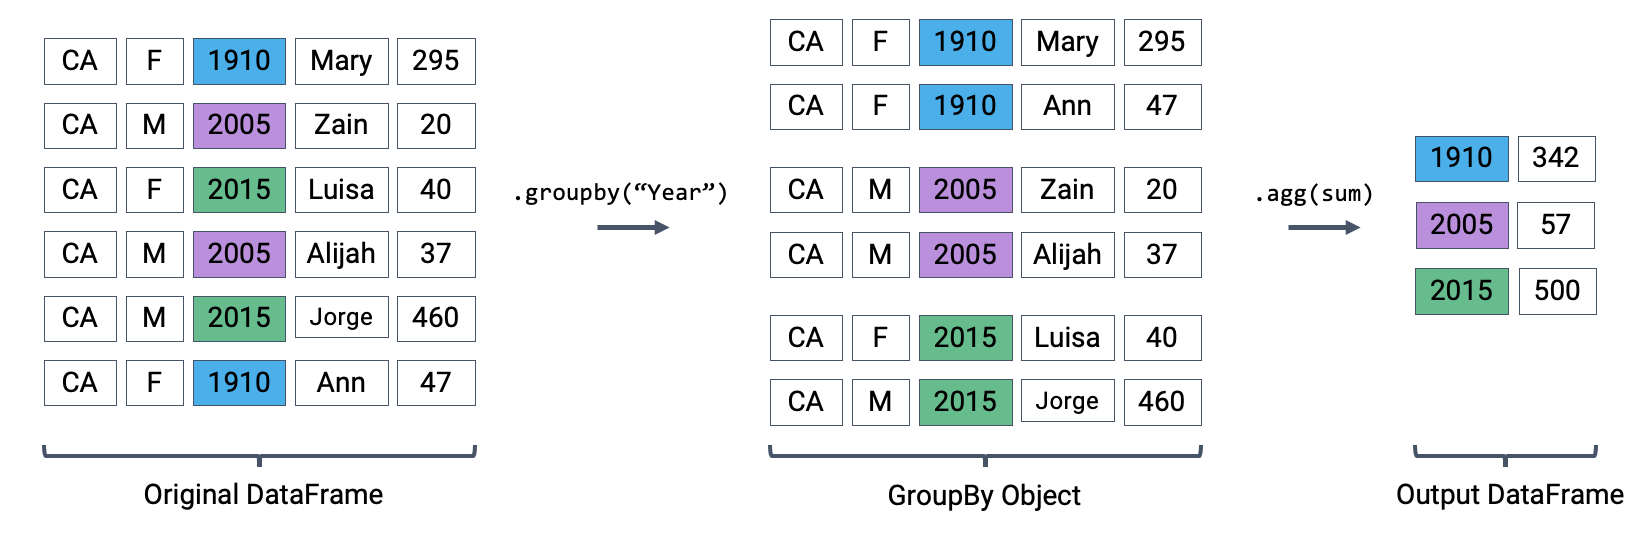
\includegraphics[keepaspectratio]{pandas_3/images/agg.png}}

}

\caption{Performing an aggregation}

\end{figure}%

Calling \texttt{.agg} has condensed each subframe back into a single
row. This gives us our final output: a \texttt{DataFrame} that is now
indexed by \texttt{"Year"}, with a single row for each unique year in
the original \texttt{babynames} DataFrame.

There are many different aggregation functions we can use, all of which
are useful in different applications.

\begin{Shaded}
\begin{Highlighting}[]
\NormalTok{babynames[[}\StringTok{"Year"}\NormalTok{, }\StringTok{"Count"}\NormalTok{]].groupby(}\StringTok{"Year"}\NormalTok{).agg(}\StringTok{"min"}\NormalTok{).head(}\DecValTok{5}\NormalTok{)}
\end{Highlighting}
\end{Shaded}

\begin{longtable}[]{@{}ll@{}}
\toprule\noalign{}
& Count \\
Year & \\
\midrule\noalign{}
\endhead
\bottomrule\noalign{}
\endlastfoot
1910 & 5 \\
1911 & 5 \\
1912 & 5 \\
1913 & 5 \\
1914 & 5 \\
\end{longtable}

\begin{Shaded}
\begin{Highlighting}[]
\NormalTok{babynames[[}\StringTok{"Year"}\NormalTok{, }\StringTok{"Count"}\NormalTok{]].groupby(}\StringTok{"Year"}\NormalTok{).agg(}\StringTok{"max"}\NormalTok{).head(}\DecValTok{5}\NormalTok{)}
\end{Highlighting}
\end{Shaded}

\begin{longtable}[]{@{}ll@{}}
\toprule\noalign{}
& Count \\
Year & \\
\midrule\noalign{}
\endhead
\bottomrule\noalign{}
\endlastfoot
1910 & 295 \\
1911 & 390 \\
1912 & 534 \\
1913 & 614 \\
1914 & 773 \\
\end{longtable}

\begin{Shaded}
\begin{Highlighting}[]
\CommentTok{\# Same result, but now we explicitly tell pandas to only consider the "Count" column when summing}
\NormalTok{babynames.groupby(}\StringTok{"Year"}\NormalTok{)[[}\StringTok{"Count"}\NormalTok{]].agg(}\StringTok{"sum"}\NormalTok{).head(}\DecValTok{5}\NormalTok{)}
\end{Highlighting}
\end{Shaded}

\begin{longtable}[]{@{}ll@{}}
\toprule\noalign{}
& Count \\
Year & \\
\midrule\noalign{}
\endhead
\bottomrule\noalign{}
\endlastfoot
1910 & 9163 \\
1911 & 9983 \\
1912 & 17946 \\
1913 & 22094 \\
1914 & 26926 \\
\end{longtable}

There are many different aggregations that can be applied to the grouped
data. The primary requirement is that an aggregation function must:

\begin{itemize}
\tightlist
\item
  Take in a \texttt{Series} of data (a single column of the grouped
  subframe).
\item
  Return a single value that aggregates this \texttt{Series}.
\end{itemize}

\subsection{Aggregation Functions}\label{aggregation-functions}

Because of this fairly broad requirement, \texttt{pandas} offers many
ways of computing an aggregation.

\textbf{In-built} Python operations -- such as \texttt{sum},
\texttt{max}, and \texttt{min} -- are automatically recognized by
\texttt{pandas}.

\begin{Shaded}
\begin{Highlighting}[]
\CommentTok{\# What is the minimum count for each name in any year?}
\NormalTok{babynames.groupby(}\StringTok{"Name"}\NormalTok{)[[}\StringTok{"Count"}\NormalTok{]].agg(}\StringTok{"min"}\NormalTok{).head()}
\end{Highlighting}
\end{Shaded}

\begin{longtable}[]{@{}ll@{}}
\toprule\noalign{}
& Count \\
Name & \\
\midrule\noalign{}
\endhead
\bottomrule\noalign{}
\endlastfoot
Aadan & 5 \\
Aadarsh & 6 \\
Aaden & 10 \\
Aadhav & 6 \\
Aadhini & 6 \\
\end{longtable}

\begin{Shaded}
\begin{Highlighting}[]
\CommentTok{\# What is the largest single{-}year count of each name?}
\NormalTok{babynames.groupby(}\StringTok{"Name"}\NormalTok{)[[}\StringTok{"Count"}\NormalTok{]].agg(}\StringTok{"max"}\NormalTok{).head()}
\end{Highlighting}
\end{Shaded}

\begin{longtable}[]{@{}ll@{}}
\toprule\noalign{}
& Count \\
Name & \\
\midrule\noalign{}
\endhead
\bottomrule\noalign{}
\endlastfoot
Aadan & 7 \\
Aadarsh & 6 \\
Aaden & 158 \\
Aadhav & 8 \\
Aadhini & 6 \\
\end{longtable}

As mentioned previously, functions from the \texttt{NumPy} library, such
as \texttt{np.mean}, \texttt{np.max}, \texttt{np.min}, and
\texttt{np.sum}, are also fair game in \texttt{pandas}.

\begin{Shaded}
\begin{Highlighting}[]
\CommentTok{\# What is the average count for each name across all years?}
\NormalTok{babynames.groupby(}\StringTok{"Name"}\NormalTok{)[[}\StringTok{"Count"}\NormalTok{]].agg(}\StringTok{"mean"}\NormalTok{).head()}
\end{Highlighting}
\end{Shaded}

\begin{longtable}[]{@{}ll@{}}
\toprule\noalign{}
& Count \\
Name & \\
\midrule\noalign{}
\endhead
\bottomrule\noalign{}
\endlastfoot
Aadan & 6.000000 \\
Aadarsh & 6.000000 \\
Aaden & 46.214286 \\
Aadhav & 6.750000 \\
Aadhini & 6.000000 \\
\end{longtable}

\texttt{pandas} also offers a number of in-built functions. Functions
that are native to \texttt{pandas} can be referenced using their string
name within a call to \texttt{.agg}. Some examples include:

\begin{itemize}
\tightlist
\item
  \texttt{.agg("sum")}
\item
  \texttt{.agg("max")}
\item
  \texttt{.agg("min")}
\item
  \texttt{.agg("mean")}
\item
  \texttt{.agg("first")}
\item
  \texttt{.agg("last")}
\end{itemize}

The latter two entries in this list -- \texttt{"first"} and
\texttt{"last"} -- are unique to \texttt{pandas}. They return the first
or last entry in a subframe column. Why might this be useful? Consider a
case where \emph{multiple} columns in a group share identical
information. To represent this information in the grouped output, we can
simply grab the first or last entry, which we know will be identical to
all other entries.

Let's illustrate this with an example. Say we add a new column to
\texttt{babynames} that contains the first letter of each name.

\begin{Shaded}
\begin{Highlighting}[]
\CommentTok{\# Imagine we had an additional column, "First Letter". We\textquotesingle{}ll explain this code next week}
\NormalTok{babynames[}\StringTok{"First Letter"}\NormalTok{] }\OperatorTok{=}\NormalTok{ babynames[}\StringTok{"Name"}\NormalTok{].}\BuiltInTok{str}\NormalTok{[}\DecValTok{0}\NormalTok{]}

\CommentTok{\# We construct a simplified DataFrame containing just a subset of columns}
\NormalTok{babynames\_new }\OperatorTok{=}\NormalTok{ babynames[[}\StringTok{"Name"}\NormalTok{, }\StringTok{"First Letter"}\NormalTok{, }\StringTok{"Year"}\NormalTok{]]}
\NormalTok{babynames\_new.head()}
\end{Highlighting}
\end{Shaded}

\begin{longtable}[]{@{}llll@{}}
\toprule\noalign{}
& Name & First Letter & Year \\
\midrule\noalign{}
\endhead
\bottomrule\noalign{}
\endlastfoot
101976 & Deandrea & D & 1986 \\
115957 & Deandrea & D & 1990 \\
308131 & Deandrea & D & 1985 \\
131029 & Leandrea & L & 1994 \\
108731 & Deandrea & D & 1988 \\
\end{longtable}

If we form groups for each name in the dataset, \texttt{"First\ Letter"}
will be the same for all members of the group. This means that if we
simply select the first entry for \texttt{"First\ Letter"} in the group,
we'll represent all data in that group.

We can use a dictionary to apply different aggregation functions to each
column during grouping.

\begin{figure}[H]

{\centering \pandocbounded{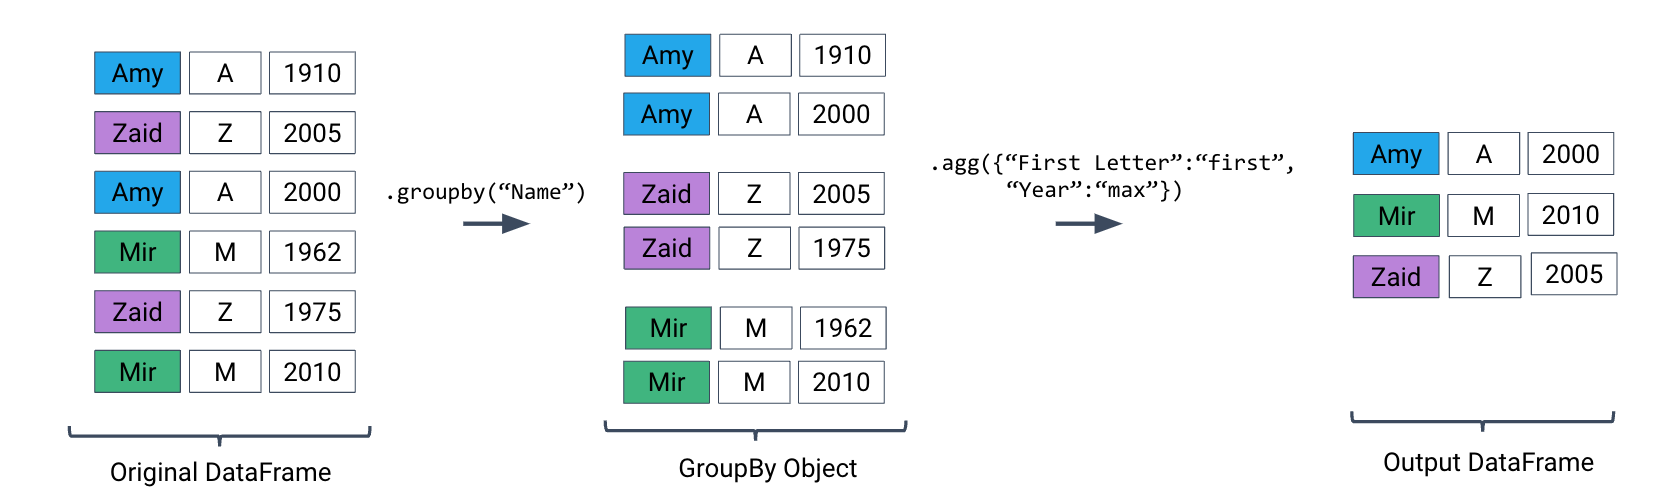
\includegraphics[keepaspectratio]{pandas_3/images/first.png}}

}

\caption{Aggregating using ``first''}

\end{figure}%

\begin{Shaded}
\begin{Highlighting}[]
\NormalTok{babynames\_new.groupby(}\StringTok{"Name"}\NormalTok{).agg(\{}\StringTok{"First Letter"}\NormalTok{:}\StringTok{"first"}\NormalTok{, }\StringTok{"Year"}\NormalTok{:}\StringTok{"max"}\NormalTok{\}).head()}
\end{Highlighting}
\end{Shaded}

\begin{longtable}[]{@{}lll@{}}
\toprule\noalign{}
& First Letter & Year \\
Name & & \\
\midrule\noalign{}
\endhead
\bottomrule\noalign{}
\endlastfoot
Aadan & A & 2014 \\
Aadarsh & A & 2019 \\
Aaden & A & 2020 \\
Aadhav & A & 2019 \\
Aadhini & A & 2022 \\
\end{longtable}

\subsection{Plotting Birth Counts}\label{plotting-birth-counts}

Let's use \texttt{.agg} to find the total number of babies born in each
year. Recall that using \texttt{.agg} with \texttt{.groupby()} follows
the format:
\texttt{df.groupby(column\_name).agg(aggregation\_function)}. The line
of code below gives us the total number of babies born in each year.

\begin{Shaded}
\begin{Highlighting}[]
\NormalTok{babynames.groupby(}\StringTok{"Year"}\NormalTok{)[[}\StringTok{"Count"}\NormalTok{]].agg(}\BuiltInTok{sum}\NormalTok{).head(}\DecValTok{5}\NormalTok{)}
\CommentTok{\# Alternative 1}
\CommentTok{\# babynames.groupby("Year")[["Count"]].sum()}
\CommentTok{\# Alternative 2}
\CommentTok{\# babynames.groupby("Year").sum(numeric\_only=True)}
\end{Highlighting}
\end{Shaded}

\begin{longtable}[]{@{}ll@{}}
\toprule\noalign{}
& Count \\
Year & \\
\midrule\noalign{}
\endhead
\bottomrule\noalign{}
\endlastfoot
1910 & 9163 \\
1911 & 9983 \\
1912 & 17946 \\
1913 & 22094 \\
1914 & 26926 \\
\end{longtable}

Here's an illustration of the process:

Plotting the \texttt{Dataframe} we obtain tells an interesting story.

\begin{Shaded}
\begin{Highlighting}[]
\ImportTok{import}\NormalTok{ plotly.express }\ImportTok{as}\NormalTok{ px}
\NormalTok{puzzle2 }\OperatorTok{=}\NormalTok{ babynames.groupby(}\StringTok{"Year"}\NormalTok{)[[}\StringTok{"Count"}\NormalTok{]].agg(}\StringTok{"sum"}\NormalTok{)}
\NormalTok{px.line(puzzle2, y }\OperatorTok{=} \StringTok{"Count"}\NormalTok{)}
\end{Highlighting}
\end{Shaded}

\begin{verbatim}
Unable to display output for mime type(s): text/html
\end{verbatim}

\begin{verbatim}
Unable to display output for mime type(s): text/html
\end{verbatim}

\textbf{A word of warning}: we made an enormous assumption when we
decided to use this dataset to estimate birth rate. According to
\href{https://lao.ca.gov/LAOEconTax/Article/Detail/691}{this article
from the Legistlative Analyst Office}, the true number of babies born in
California in 2020 was 421,275. However, our plot shows 362,882 babies
------ what happened?

\subsection{\texorpdfstring{Summary of the \texttt{.groupby()}
Function}{Summary of the .groupby() Function}}\label{summary-of-the-.groupby-function}

A \texttt{groupby} operation involves some combination of
\textbf{splitting a \texttt{DataFrame} into grouped subframes},
\textbf{applying a function}, and \textbf{combining the results}.

For some arbitrary \texttt{DataFrame} \texttt{df} below, the code
\texttt{df.groupby("year").agg(sum)} does the following:

\begin{itemize}
\tightlist
\item
  \textbf{Splits} the \texttt{DataFrame} into sub-\texttt{DataFrame}s
  with rows belonging to the same year.
\item
  \textbf{Applies} the \texttt{sum} function to each column of each
  sub-\texttt{DataFrame}.
\item
  \textbf{Combines} the results of \texttt{sum} into a single
  \texttt{DataFrame}, indexed by \texttt{year}.
\end{itemize}

\subsection{\texorpdfstring{Revisiting the \texttt{.agg()}
Function}{Revisiting the .agg() Function}}\label{revisiting-the-.agg-function}

\texttt{.agg()} can take in any function that aggregates several values
into one summary value. Some commonly-used aggregation functions can
even be called directly, without explicit use of \texttt{.agg()}. For
example, we can call \texttt{.mean()} on \texttt{.groupby()}:

\begin{verbatim}
babynames.groupby("Year").mean().head()
\end{verbatim}

We can now put this all into practice. Say we want to find the baby name
with sex ``F'' that has fallen in popularity the most in California. To
calculate this, we can first create a metric: ``Ratio to Peak'' (RTP).
The RTP is the ratio of babies born with a given name in 2022 to the
\emph{maximum} number of babies born with the name in \emph{any} year.

Let's start with calculating this for one baby, ``Jennifer''.

\begin{Shaded}
\begin{Highlighting}[]
\CommentTok{\# We filter by babies with sex "F" and sort by "Year"}
\NormalTok{f\_babynames }\OperatorTok{=}\NormalTok{ babynames[babynames[}\StringTok{"Sex"}\NormalTok{] }\OperatorTok{==} \StringTok{"F"}\NormalTok{]}
\NormalTok{f\_babynames }\OperatorTok{=}\NormalTok{ f\_babynames.sort\_values([}\StringTok{"Year"}\NormalTok{])}

\CommentTok{\# Determine how many Jennifers were born in CA per year}
\NormalTok{jenn\_counts\_series }\OperatorTok{=}\NormalTok{ f\_babynames[f\_babynames[}\StringTok{"Name"}\NormalTok{] }\OperatorTok{==} \StringTok{"Jennifer"}\NormalTok{][}\StringTok{"Count"}\NormalTok{]}

\CommentTok{\# Determine the max number of Jennifers born in a year and the number born in 2022 }
\CommentTok{\# to calculate RTP}
\NormalTok{max\_jenn }\OperatorTok{=} \BuiltInTok{max}\NormalTok{(f\_babynames[f\_babynames[}\StringTok{"Name"}\NormalTok{] }\OperatorTok{==} \StringTok{"Jennifer"}\NormalTok{][}\StringTok{"Count"}\NormalTok{])}
\NormalTok{curr\_jenn }\OperatorTok{=}\NormalTok{ f\_babynames[f\_babynames[}\StringTok{"Name"}\NormalTok{] }\OperatorTok{==} \StringTok{"Jennifer"}\NormalTok{][}\StringTok{"Count"}\NormalTok{].iloc[}\OperatorTok{{-}}\DecValTok{1}\NormalTok{]}
\NormalTok{rtp }\OperatorTok{=}\NormalTok{ curr\_jenn }\OperatorTok{/}\NormalTok{ max\_jenn}
\NormalTok{rtp}
\end{Highlighting}
\end{Shaded}

\begin{verbatim}
np.float64(0.018796372629843364)
\end{verbatim}

By creating a function to calculate RTP and applying it to our
\texttt{DataFrame} by using \texttt{.groupby()}, we can easily compute
the RTP for all names at once!

\begin{Shaded}
\begin{Highlighting}[]
\KeywordTok{def}\NormalTok{ ratio\_to\_peak(series):}
    \ControlFlowTok{return}\NormalTok{ series.iloc[}\OperatorTok{{-}}\DecValTok{1}\NormalTok{] }\OperatorTok{/} \BuiltInTok{max}\NormalTok{(series)}

\CommentTok{\#Using .groupby() to apply the function}
\NormalTok{rtp\_table }\OperatorTok{=}\NormalTok{ f\_babynames.groupby(}\StringTok{"Name"}\NormalTok{)[[}\StringTok{"Year"}\NormalTok{, }\StringTok{"Count"}\NormalTok{]].agg(ratio\_to\_peak)}
\NormalTok{rtp\_table.head()}
\end{Highlighting}
\end{Shaded}

\begin{longtable}[]{@{}lll@{}}
\toprule\noalign{}
& Year & Count \\
Name & & \\
\midrule\noalign{}
\endhead
\bottomrule\noalign{}
\endlastfoot
Aadhini & 1.0 & 1.000000 \\
Aadhira & 1.0 & 0.500000 \\
Aadhya & 1.0 & 0.660000 \\
Aadya & 1.0 & 0.586207 \\
Aahana & 1.0 & 0.269231 \\
\end{longtable}

In the rows shown above, we can see that every row shown has a
\texttt{Year} value of \texttt{1.0}.

This is the ``\textbf{\texttt{pandas}}-ification'' of logic you saw in
Data 8. Much of the logic you've learned in Data 8 will serve you well
in Data 100.

\subsection{Nuisance Columns}\label{nuisance-columns}

Note that you must be careful with which columns you apply the
\texttt{.agg()} function to. If we were to apply our function to the
table as a whole by doing
\texttt{f\_babynames.groupby("Name").agg(ratio\_to\_peak)}, executing
our \texttt{.agg()} call would result in a \texttt{TypeError}.

We can avoid this issue (and prevent unintentional loss of data) by
explicitly selecting column(s) we want to apply our aggregation function
to \textbf{BEFORE} calling \texttt{.agg()},

\subsection{Renaming Columns After
Grouping}\label{renaming-columns-after-grouping}

By default, \texttt{.groupby} will not rename any aggregated columns. As
we can see in the table above, the aggregated column is still named
\texttt{Count} even though it now represents the RTP. For better
readability, we can rename \texttt{Count} to \texttt{Count\ RTP}

\begin{Shaded}
\begin{Highlighting}[]
\NormalTok{rtp\_table }\OperatorTok{=}\NormalTok{ rtp\_table.rename(columns }\OperatorTok{=}\NormalTok{ \{}\StringTok{"Count"}\NormalTok{: }\StringTok{"Count RTP"}\NormalTok{\})}
\NormalTok{rtp\_table}
\end{Highlighting}
\end{Shaded}

\begin{longtable}[]{@{}lll@{}}
\toprule\noalign{}
& Year & Count RTP \\
Name & & \\
\midrule\noalign{}
\endhead
\bottomrule\noalign{}
\endlastfoot
Aadhini & 1.0 & 1.000000 \\
Aadhira & 1.0 & 0.500000 \\
Aadhya & 1.0 & 0.660000 \\
Aadya & 1.0 & 0.586207 \\
Aahana & 1.0 & 0.269231 \\
... & ... & ... \\
Zyanya & 1.0 & 0.466667 \\
Zyla & 1.0 & 1.000000 \\
Zylah & 1.0 & 1.000000 \\
Zyra & 1.0 & 1.000000 \\
Zyrah & 1.0 & 0.833333 \\
\end{longtable}

\subsection{Some Data Science Payoff}\label{some-data-science-payoff}

By sorting \texttt{rtp\_table}, we can see the names whose popularity
has decreased the most.

\begin{Shaded}
\begin{Highlighting}[]
\NormalTok{rtp\_table }\OperatorTok{=}\NormalTok{ rtp\_table.rename(columns }\OperatorTok{=}\NormalTok{ \{}\StringTok{"Count"}\NormalTok{: }\StringTok{"Count RTP"}\NormalTok{\})}
\NormalTok{rtp\_table.sort\_values(}\StringTok{"Count RTP"}\NormalTok{).head()}
\end{Highlighting}
\end{Shaded}

\begin{longtable}[]{@{}lll@{}}
\toprule\noalign{}
& Year & Count RTP \\
Name & & \\
\midrule\noalign{}
\endhead
\bottomrule\noalign{}
\endlastfoot
Debra & 1.0 & 0.001260 \\
Debbie & 1.0 & 0.002815 \\
Carol & 1.0 & 0.003180 \\
Tammy & 1.0 & 0.003249 \\
Susan & 1.0 & 0.003305 \\
\end{longtable}

To visualize the above \texttt{DataFrame}, let's look at the line plot
below:

\begin{Shaded}
\begin{Highlighting}[]
\ImportTok{import}\NormalTok{ plotly.express }\ImportTok{as}\NormalTok{ px}
\NormalTok{px.line(f\_babynames[f\_babynames[}\StringTok{"Name"}\NormalTok{] }\OperatorTok{==} \StringTok{"Debra"}\NormalTok{], x }\OperatorTok{=} \StringTok{"Year"}\NormalTok{, y }\OperatorTok{=} \StringTok{"Count"}\NormalTok{)}
\end{Highlighting}
\end{Shaded}

\begin{verbatim}
Unable to display output for mime type(s): text/html
\end{verbatim}

We can get the list of the top 10 names and then plot popularity with
the following code:

\begin{Shaded}
\begin{Highlighting}[]
\NormalTok{top10 }\OperatorTok{=}\NormalTok{ rtp\_table.sort\_values(}\StringTok{"Count RTP"}\NormalTok{).head(}\DecValTok{10}\NormalTok{).index}
\NormalTok{px.line(}
\NormalTok{    f\_babynames[f\_babynames[}\StringTok{"Name"}\NormalTok{].isin(top10)], }
\NormalTok{    x }\OperatorTok{=} \StringTok{"Year"}\NormalTok{, }
\NormalTok{    y }\OperatorTok{=} \StringTok{"Count"}\NormalTok{, }
\NormalTok{    color }\OperatorTok{=} \StringTok{"Name"}
\NormalTok{)}
\end{Highlighting}
\end{Shaded}

\begin{verbatim}
Unable to display output for mime type(s): text/html
\end{verbatim}

As a quick exercise, consider what code would compute the total number
of babies with each name.

\begin{Shaded}
\begin{Highlighting}[]
\NormalTok{babynames.groupby(}\StringTok{"Name"}\NormalTok{)[[}\StringTok{"Count"}\NormalTok{]].agg(}\StringTok{"sum"}\NormalTok{).head()}
\CommentTok{\# alternative solution: }
\CommentTok{\# babynames.groupby("Name")[["Count"]].sum()}
\end{Highlighting}
\end{Shaded}

\begin{longtable}[]{@{}ll@{}}
\toprule\noalign{}
& Count \\
Name & \\
\midrule\noalign{}
\endhead
\bottomrule\noalign{}
\endlastfoot
Aadan & 18 \\
Aadarsh & 6 \\
Aaden & 647 \\
Aadhav & 27 \\
Aadhini & 6 \\
\end{longtable}

\section{\texorpdfstring{\texttt{.groupby()},
Continued}{.groupby(), Continued}}\label{groupby-continued}

We'll work with the \texttt{elections} \texttt{DataFrame} again.

\begin{Shaded}
\begin{Highlighting}[]
\ImportTok{import}\NormalTok{ pandas }\ImportTok{as}\NormalTok{ pd}
\ImportTok{import}\NormalTok{ numpy }\ImportTok{as}\NormalTok{ np}

\NormalTok{elections }\OperatorTok{=}\NormalTok{ pd.read\_csv(}\StringTok{"data/elections.csv"}\NormalTok{)}
\NormalTok{elections.head(}\DecValTok{5}\NormalTok{)}
\end{Highlighting}
\end{Shaded}

\begin{longtable}[]{@{}lllllll@{}}
\toprule\noalign{}
& Year & Candidate & Party & Popular vote & Result & \% \\
\midrule\noalign{}
\endhead
\bottomrule\noalign{}
\endlastfoot
0 & 1824 & Andrew Jackson & Democratic-Republican & 151271 & loss &
57.210122 \\
1 & 1824 & John Quincy Adams & Democratic-Republican & 113142 & win &
42.789878 \\
2 & 1828 & Andrew Jackson & Democratic & 642806 & win & 56.203927 \\
3 & 1828 & John Quincy Adams & National Republican & 500897 & loss &
43.796073 \\
4 & 1832 & Andrew Jackson & Democratic & 702735 & win & 54.574789 \\
\end{longtable}

\subsection{\texorpdfstring{Raw \texttt{GroupBy}
Objects}{Raw GroupBy Objects}}\label{raw-groupby-objects}

The result of \texttt{groupby} applied to a \texttt{DataFrame} is a
\texttt{DataFrameGroupBy} object, \textbf{not} a \texttt{DataFrame}.

\begin{Shaded}
\begin{Highlighting}[]
\NormalTok{grouped\_by\_year }\OperatorTok{=}\NormalTok{ elections.groupby(}\StringTok{"Year"}\NormalTok{)}
\BuiltInTok{type}\NormalTok{(grouped\_by\_year)}
\end{Highlighting}
\end{Shaded}

\begin{verbatim}
pandas.core.groupby.generic.DataFrameGroupBy
\end{verbatim}

There are several ways to look into \texttt{DataFrameGroupBy} objects:

\begin{Shaded}
\begin{Highlighting}[]
\NormalTok{grouped\_by\_party }\OperatorTok{=}\NormalTok{ elections.groupby(}\StringTok{"Party"}\NormalTok{)}
\NormalTok{grouped\_by\_party.groups}
\end{Highlighting}
\end{Shaded}

\begin{verbatim}
{'American': [22, 126], 'American Independent': [115, 119, 124], 'Anti-Masonic': [6], 'Anti-Monopoly': [38], 'Citizens': [127], 'Communist': [89], 'Constitution': [160, 164, 172], 'Constitutional Union': [24], 'Democratic': [2, 4, 8, 10, 13, 14, 17, 20, 28, 29, 34, 37, 39, 45, 47, 52, 55, 57, 64, 70, 74, 77, 81, 83, 86, 91, 94, 97, 100, 105, 108, 111, 114, 116, 118, 123, 129, 134, 137, 140, 144, 151, 158, 162, 168, 176, 178, 183], 'Democratic-Republican': [0, 1], 'Dixiecrat': [103], 'Farmer–Labor': [78], 'Free Soil': [15, 18], 'Green': [149, 155, 156, 165, 170, 177, 181, 184], 'Greenback': [35], 'Independent': [121, 130, 143, 161, 167, 174, 185], 'Liberal Republican': [31], 'Libertarian': [125, 128, 132, 138, 139, 146, 153, 159, 163, 169, 175, 180], 'Libertarian Party': [186], 'National Democratic': [50], 'National Republican': [3, 5], 'National Union': [27], 'Natural Law': [148], 'New Alliance': [136], 'Northern Democratic': [26], 'Populist': [48, 61, 141], 'Progressive': [68, 82, 101, 107], 'Prohibition': [41, 44, 49, 51, 54, 59, 63, 67, 73, 75, 99], 'Reform': [150, 154], 'Republican': [21, 23, 30, 32, 33, 36, 40, 43, 46, 53, 56, 60, 65, 69, 72, 79, 80, 84, 87, 90, 96, 98, 104, 106, 109, 112, 113, 117, 120, 122, 131, 133, 135, 142, 145, 152, 157, 166, 171, 173, 179, 182], 'Socialist': [58, 62, 66, 71, 76, 85, 88, 92, 95, 102], 'Southern Democratic': [25], 'States' Rights': [110], 'Taxpayers': [147], 'Union': [93], 'Union Labor': [42], 'Whig': [7, 9, 11, 12, 16, 19]}
\end{verbatim}

\begin{Shaded}
\begin{Highlighting}[]
\NormalTok{grouped\_by\_party.get\_group(}\StringTok{"Socialist"}\NormalTok{)}
\end{Highlighting}
\end{Shaded}

\begin{longtable}[]{@{}lllllll@{}}
\toprule\noalign{}
& Year & Candidate & Party & Popular vote & Result & \% \\
\midrule\noalign{}
\endhead
\bottomrule\noalign{}
\endlastfoot
58 & 1904 & Eugene V. Debs & Socialist & 402810 & loss & 2.985897 \\
62 & 1908 & Eugene V. Debs & Socialist & 420852 & loss & 2.850866 \\
66 & 1912 & Eugene V. Debs & Socialist & 901551 & loss & 6.004354 \\
71 & 1916 & Allan L. Benson & Socialist & 590524 & loss & 3.194193 \\
76 & 1920 & Eugene V. Debs & Socialist & 913693 & loss & 3.428282 \\
85 & 1928 & Norman Thomas & Socialist & 267478 & loss & 0.728623 \\
88 & 1932 & Norman Thomas & Socialist & 884885 & loss & 2.236211 \\
92 & 1936 & Norman Thomas & Socialist & 187910 & loss & 0.412876 \\
95 & 1940 & Norman Thomas & Socialist & 116599 & loss & 0.234237 \\
102 & 1948 & Norman Thomas & Socialist & 139569 & loss & 0.286312 \\
\end{longtable}

\subsection{\texorpdfstring{Other \texttt{GroupBy}
Methods}{Other GroupBy Methods}}\label{other-groupby-methods}

There are many aggregation methods we can use with \texttt{.agg}. Some
useful options are:

\begin{itemize}
\tightlist
\item
  \href{https://pandas.pydata.org/docs/reference/api/pandas.core.groupby.DataFrameGroupBy.mean.html\#pandas.core.groupby.DataFrameGroupBy.mean}{\texttt{.mean}}:
  creates a new \texttt{DataFrame} with the mean value of each group
\item
  \href{https://pandas.pydata.org/docs/reference/api/pandas.core.groupby.DataFrameGroupBy.sum.html\#pandas.core.groupby.DataFrameGroupBy.sum}{\texttt{.sum}}:
  creates a new \texttt{DataFrame} with the sum of each group
\item
  \href{https://pandas.pydata.org/docs/reference/api/pandas.core.groupby.DataFrameGroupBy.max.html\#pandas.core.groupby.DataFrameGroupBy.max}{\texttt{.max}}
  and
  \href{https://pandas.pydata.org/docs/reference/api/pandas.core.groupby.DataFrameGroupBy.min.html\#pandas.core.groupby.DataFrameGroupBy.min}{\texttt{.min}}:
  creates a new \texttt{DataFrame} with the maximum/minimum value of
  each group
\item
  \href{https://pandas.pydata.org/docs/reference/api/pandas.core.groupby.DataFrameGroupBy.first.html\#pandas.core.groupby.DataFrameGroupBy.first}{\texttt{.first}}
  and
  \href{https://pandas.pydata.org/docs/reference/api/pandas.core.groupby.DataFrameGroupBy.last.html\#pandas.core.groupby.DataFrameGroupBy.last}{\texttt{.last}}:
  creates a new \texttt{DataFrame} with the first/last row in each group
\item
  \href{https://pandas.pydata.org/docs/reference/api/pandas.core.groupby.DataFrameGroupBy.size.html\#pandas.core.groupby.DataFrameGroupBy.size}{\texttt{.size}}:
  creates a new \textbf{\texttt{Series}} with the number of entries in
  each group
\item
  \href{https://pandas.pydata.org/docs/reference/api/pandas.core.groupby.DataFrameGroupBy.count.html\#pandas.core.groupby.DataFrameGroupBy.count}{\texttt{.count}}:
  creates a new \textbf{\texttt{DataFrame}} with the number of entries,
  excluding missing values.
\end{itemize}

Let's illustrate some examples by creating a \texttt{DataFrame} called
\texttt{df}.

\begin{Shaded}
\begin{Highlighting}[]
\NormalTok{df }\OperatorTok{=}\NormalTok{ pd.DataFrame(\{}\StringTok{\textquotesingle{}letter\textquotesingle{}}\NormalTok{:[}\StringTok{\textquotesingle{}A\textquotesingle{}}\NormalTok{,}\StringTok{\textquotesingle{}A\textquotesingle{}}\NormalTok{,}\StringTok{\textquotesingle{}B\textquotesingle{}}\NormalTok{,}\StringTok{\textquotesingle{}C\textquotesingle{}}\NormalTok{,}\StringTok{\textquotesingle{}C\textquotesingle{}}\NormalTok{,}\StringTok{\textquotesingle{}C\textquotesingle{}}\NormalTok{], }
                   \StringTok{\textquotesingle{}num\textquotesingle{}}\NormalTok{:[}\DecValTok{1}\NormalTok{,}\DecValTok{2}\NormalTok{,}\DecValTok{3}\NormalTok{,}\DecValTok{4}\NormalTok{,np.nan,}\DecValTok{4}\NormalTok{], }
                   \StringTok{\textquotesingle{}state\textquotesingle{}}\NormalTok{:[np.nan, }\StringTok{\textquotesingle{}tx\textquotesingle{}}\NormalTok{, }\StringTok{\textquotesingle{}fl\textquotesingle{}}\NormalTok{, }\StringTok{\textquotesingle{}hi\textquotesingle{}}\NormalTok{, np.nan, }\StringTok{\textquotesingle{}ak\textquotesingle{}}\NormalTok{]\})}
\NormalTok{df}
\end{Highlighting}
\end{Shaded}

\begin{longtable}[]{@{}llll@{}}
\toprule\noalign{}
& letter & num & state \\
\midrule\noalign{}
\endhead
\bottomrule\noalign{}
\endlastfoot
0 & A & 1.0 & NaN \\
1 & A & 2.0 & tx \\
2 & B & 3.0 & fl \\
3 & C & 4.0 & hi \\
4 & C & NaN & NaN \\
5 & C & 4.0 & ak \\
\end{longtable}

Note the slight difference between \texttt{.size()} and
\texttt{.count()}: while \texttt{.size()} returns a \texttt{Series} and
counts the number of entries including the missing values,
\texttt{.count()} returns a \texttt{DataFrame} and counts the number of
entries in each column \emph{excluding missing values}.

\begin{Shaded}
\begin{Highlighting}[]
\NormalTok{df.groupby(}\StringTok{"letter"}\NormalTok{).size()}
\end{Highlighting}
\end{Shaded}

\begin{verbatim}
letter
A    2
B    1
C    3
dtype: int64
\end{verbatim}

\begin{Shaded}
\begin{Highlighting}[]
\NormalTok{df.groupby(}\StringTok{"letter"}\NormalTok{).count()}
\end{Highlighting}
\end{Shaded}

\begin{longtable}[]{@{}lll@{}}
\toprule\noalign{}
& num & state \\
letter & & \\
\midrule\noalign{}
\endhead
\bottomrule\noalign{}
\endlastfoot
A & 2 & 1 \\
B & 1 & 1 \\
C & 2 & 2 \\
\end{longtable}

You might recall that the \texttt{value\_counts()} function in the
previous note does something similar. It turns out
\texttt{value\_counts()} and \texttt{groupby.size()} are the same,
except \texttt{value\_counts()} sorts the resulting \texttt{Series} in
descending order automatically.

\begin{Shaded}
\begin{Highlighting}[]
\NormalTok{df[}\StringTok{"letter"}\NormalTok{].value\_counts()}
\end{Highlighting}
\end{Shaded}

\begin{verbatim}
letter
C    3
A    2
B    1
Name: count, dtype: int64
\end{verbatim}

These (and other) aggregation functions are so common that
\texttt{pandas} allows for writing shorthand. Instead of explicitly
stating the use of \texttt{.agg}, we can call the function directly on
the \texttt{GroupBy} object.

For example, the following are equivalent:

\begin{itemize}
\tightlist
\item
  \texttt{elections.groupby("Candidate").agg(mean)}
\item
  \texttt{elections.groupby("Candidate").mean()}
\end{itemize}

There are many other methods that \texttt{pandas} supports. You can
check them out on the
\href{https://pandas.pydata.org/docs/reference/groupby.html}{\texttt{pandas}
documentation}.

\subsection{Filtering by Group}\label{filtering-by-group}

Another common use for \texttt{GroupBy} objects is to filter data by
group.

\texttt{groupby.filter} takes an argument \texttt{func}, where
\texttt{func} is a function that:

\begin{itemize}
\tightlist
\item
  Takes a \texttt{DataFrame} object as input
\item
  Returns a single \texttt{True} or \texttt{False}.
\end{itemize}

\texttt{groupby.filter} applies \texttt{func} to each
group/sub-\texttt{DataFrame}:

\begin{itemize}
\tightlist
\item
  If \texttt{func} returns \texttt{True} for a group, then all rows
  belonging to the group are preserved.
\item
  If \texttt{func} returns \texttt{False} for a group, then all rows
  belonging to that group are filtered out.
\end{itemize}

In other words, sub-\texttt{DataFrame}s that correspond to \texttt{True}
are returned in the final result, whereas those with a \texttt{False}
value are not. Importantly, \texttt{groupby.filter} is different from
\texttt{groupby.agg} in that an \emph{entire} sub-\texttt{DataFrame} is
returned in the final \texttt{DataFrame}, not just a single row. As a
result, \texttt{groupby.filter} preserves the original indices and the
column we grouped on does \textbf{NOT} become the index!

To illustrate how this happens, let's go back to the \texttt{elections}
dataset. Say we want to identify ``tight'' election years -- that is, we
want to find all rows that correspond to election years where all
candidates in that year won a similar portion of the total vote.
Specifically, let's find all rows corresponding to a year where no
candidate won more than 45\% of the total vote.

In other words, we want to:

\begin{itemize}
\tightlist
\item
  Find the years where the maximum \texttt{\%} in that year is less than
  45\%
\item
  Return all \texttt{DataFrame} rows that correspond to these years
\end{itemize}

For each year, we need to find the maximum \texttt{\%} among \emph{all}
rows for that year. If this maximum \texttt{\%} is lower than 45\%, we
will tell \texttt{pandas} to keep all rows corresponding to that year.

\begin{Shaded}
\begin{Highlighting}[]
\NormalTok{elections.groupby(}\StringTok{"Year"}\NormalTok{).}\BuiltInTok{filter}\NormalTok{(}\KeywordTok{lambda}\NormalTok{ sf: sf[}\StringTok{"\%"}\NormalTok{].}\BuiltInTok{max}\NormalTok{() }\OperatorTok{\textless{}} \DecValTok{45}\NormalTok{).head(}\DecValTok{9}\NormalTok{)}
\end{Highlighting}
\end{Shaded}

\begin{longtable}[]{@{}lllllll@{}}
\toprule\noalign{}
& Year & Candidate & Party & Popular vote & Result & \% \\
\midrule\noalign{}
\endhead
\bottomrule\noalign{}
\endlastfoot
23 & 1860 & Abraham Lincoln & Republican & 1855993 & win & 39.699408 \\
24 & 1860 & John Bell & Constitutional Union & 590901 & loss &
12.639283 \\
25 & 1860 & John C. Breckinridge & Southern Democratic & 848019 & loss &
18.138998 \\
26 & 1860 & Stephen A. Douglas & Northern Democratic & 1380202 & loss &
29.522311 \\
66 & 1912 & Eugene V. Debs & Socialist & 901551 & loss & 6.004354 \\
67 & 1912 & Eugene W. Chafin & Prohibition & 208156 & loss & 1.386325 \\
68 & 1912 & Theodore Roosevelt & Progressive & 4122721 & loss &
27.457433 \\
69 & 1912 & William Taft & Republican & 3486242 & loss & 23.218466 \\
70 & 1912 & Woodrow Wilson & Democratic & 6296284 & win & 41.933422 \\
\end{longtable}

What's going on here? In this example, we've defined our filtering
function, \texttt{func}, to be
\texttt{lambda\ sf:\ sf{[}"\%"{]}.max()\ \textless{}\ 45}. This
filtering function will find the maximum \texttt{"\%"} value among all
entries in the grouped sub-\texttt{DataFrame}, which we call
\texttt{sf}. If the maximum value is less than 45, then the filter
function will return \texttt{True} and all rows in that grouped
sub-\texttt{DataFrame} will appear in the final output
\texttt{DataFrame}.

Examine the \texttt{DataFrame} above. Notice how, in this preview of the
first 9 rows, all entries from the years 1860 and 1912 appear. This
means that in 1860 and 1912, no candidate in that year won more than
45\% of the total vote.

You may ask: how is the \texttt{groupby.filter} procedure different to
the boolean filtering we've seen previously? Boolean filtering considers
\emph{individual} rows when applying a boolean condition. For example,
the code \texttt{elections{[}elections{[}"\%"{]}\ \textless{}\ 45{]}}
will check the \texttt{"\%"} value of every single row in
\texttt{elections}; if it is less than 45, then that row will be kept in
the output. \texttt{groupby.filter}, in contrast, applies a boolean
condition \emph{across} all rows in a group. If not all rows in that
group satisfy the condition specified by the filter, the entire group
will be discarded in the output.

\subsection{\texorpdfstring{Aggregation with \texttt{lambda}
Functions}{Aggregation with lambda Functions}}\label{aggregation-with-lambda-functions}

What if we wish to aggregate our \texttt{DataFrame} using a non-standard
function -- for example, a function of our own design? We can do so by
combining \texttt{.agg} with \texttt{lambda} expressions.

Let's first consider a puzzle to jog our memory. We will attempt to find
the \texttt{Candidate} from each \texttt{Party} with the highest
\texttt{\%} of votes.

A naive approach may be to group by the \texttt{Party} column and
aggregate by the maximum.

\begin{Shaded}
\begin{Highlighting}[]
\NormalTok{elections.groupby(}\StringTok{"Party"}\NormalTok{).agg(}\BuiltInTok{max}\NormalTok{).head(}\DecValTok{10}\NormalTok{)}
\end{Highlighting}
\end{Shaded}

\begin{longtable}[]{@{}llllll@{}}
\toprule\noalign{}
& Year & Candidate & Popular vote & Result & \% \\
Party & & & & & \\
\midrule\noalign{}
\endhead
\bottomrule\noalign{}
\endlastfoot
American & 1976 & Thomas J. Anderson & 873053 & loss & 21.554001 \\
American Independent & 1976 & Lester Maddox & 9901118 & loss &
13.571218 \\
Anti-Masonic & 1832 & William Wirt & 100715 & loss & 7.821583 \\
Anti-Monopoly & 1884 & Benjamin Butler & 134294 & loss & 1.335838 \\
Citizens & 1980 & Barry Commoner & 233052 & loss & 0.270182 \\
Communist & 1932 & William Z. Foster & 103307 & loss & 0.261069 \\
Constitution & 2016 & Michael Peroutka & 203091 & loss & 0.152398 \\
Constitutional Union & 1860 & John Bell & 590901 & loss & 12.639283 \\
Democratic & 2024 & Woodrow Wilson & 81268924 & win & 61.344703 \\
Democratic-Republican & 1824 & John Quincy Adams & 151271 & win &
57.210122 \\
\end{longtable}

This approach is clearly wrong -- the \texttt{DataFrame} claims that
Woodrow Wilson won the presidency in 2020.

Why is this happening? Here, the \texttt{max} aggregation function is
taken over every column \emph{independently}. Among Democrats,
\texttt{max} is computing:

\begin{itemize}
\tightlist
\item
  The most recent \texttt{Year} a Democratic candidate ran for president
  (2020)
\item
  The \texttt{Candidate} with the alphabetically ``largest'' name
  (``Woodrow Wilson'')
\item
  The \texttt{Result} with the alphabetically ``largest'' outcome
  (``win'')
\end{itemize}

Instead, let's try a different approach. We will:

\begin{enumerate}
\def\labelenumi{\arabic{enumi}.}
\tightlist
\item
  Sort the \texttt{DataFrame} so that rows are in descending order of
  \texttt{\%}
\item
  Group by \texttt{Party} and select the first row of each
  sub-\texttt{DataFrame}
\end{enumerate}

While it may seem unintuitive, sorting \texttt{elections} by descending
order of \texttt{\%} is extremely helpful. If we then group by
\texttt{Party}, the first row of each \texttt{GroupBy} object will
contain information about the \texttt{Candidate} with the highest voter
\texttt{\%}.

\begin{Shaded}
\begin{Highlighting}[]
\NormalTok{elections\_sorted\_by\_percent }\OperatorTok{=}\NormalTok{ elections.sort\_values(}\StringTok{"\%"}\NormalTok{, ascending}\OperatorTok{=}\VariableTok{False}\NormalTok{)}
\NormalTok{elections\_sorted\_by\_percent.head(}\DecValTok{5}\NormalTok{)}
\end{Highlighting}
\end{Shaded}

\begin{longtable}[]{@{}lllllll@{}}
\toprule\noalign{}
& Year & Candidate & Party & Popular vote & Result & \% \\
\midrule\noalign{}
\endhead
\bottomrule\noalign{}
\endlastfoot
114 & 1964 & Lyndon Johnson & Democratic & 43127041 & win & 61.344703 \\
91 & 1936 & Franklin Roosevelt & Democratic & 27752648 & win &
60.978107 \\
120 & 1972 & Richard Nixon & Republican & 47168710 & win & 60.907806 \\
79 & 1920 & Warren Harding & Republican & 16144093 & win & 60.574501 \\
133 & 1984 & Ronald Reagan & Republican & 54455472 & win & 59.023326 \\
\end{longtable}

\begin{Shaded}
\begin{Highlighting}[]
\NormalTok{elections\_sorted\_by\_percent.groupby(}\StringTok{"Party"}\NormalTok{).agg(}\KeywordTok{lambda}\NormalTok{ x : x.iloc[}\DecValTok{0}\NormalTok{]).head(}\DecValTok{10}\NormalTok{)}

\CommentTok{\# Equivalent to the below code}
\CommentTok{\# elections\_sorted\_by\_percent.groupby("Party").agg(\textquotesingle{}first\textquotesingle{}).head(10)}
\end{Highlighting}
\end{Shaded}

\begin{longtable}[]{@{}llllll@{}}
\toprule\noalign{}
& Year & Candidate & Popular vote & Result & \% \\
Party & & & & & \\
\midrule\noalign{}
\endhead
\bottomrule\noalign{}
\endlastfoot
American & 1856 & Millard Fillmore & 873053 & loss & 21.554001 \\
American Independent & 1968 & George Wallace & 9901118 & loss &
13.571218 \\
Anti-Masonic & 1832 & William Wirt & 100715 & loss & 7.821583 \\
Anti-Monopoly & 1884 & Benjamin Butler & 134294 & loss & 1.335838 \\
Citizens & 1980 & Barry Commoner & 233052 & loss & 0.270182 \\
Communist & 1932 & William Z. Foster & 103307 & loss & 0.261069 \\
Constitution & 2008 & Chuck Baldwin & 199750 & loss & 0.152398 \\
Constitutional Union & 1860 & John Bell & 590901 & loss & 12.639283 \\
Democratic & 1964 & Lyndon Johnson & 43127041 & win & 61.344703 \\
Democratic-Republican & 1824 & Andrew Jackson & 151271 & loss &
57.210122 \\
\end{longtable}

Here's an illustration of the process:

Notice how our code correctly determines that Lyndon Johnson from the
Democratic Party has the highest voter \texttt{\%}.

More generally, \texttt{lambda} functions are used to design custom
aggregation functions that aren't pre-defined by Python. The input
parameter \texttt{x} to the \texttt{lambda} function is a
\texttt{GroupBy} object. Therefore, it should make sense why
\texttt{lambda\ x\ :\ x.iloc{[}0{]}} selects the first row in each
groupby object.

In fact, there's a few different ways to approach this problem. Each
approach has different tradeoffs in terms of readability, performance,
memory consumption, complexity, etc. We've given a few examples below.

\textbf{Note}: Understanding these alternative solutions is not
required. They are given to demonstrate the vast number of
problem-solving approaches in \texttt{pandas}.

\begin{Shaded}
\begin{Highlighting}[]
\CommentTok{\# Using the idxmax function}
\NormalTok{best\_per\_party }\OperatorTok{=}\NormalTok{ elections.loc[elections.groupby(}\StringTok{\textquotesingle{}Party\textquotesingle{}}\NormalTok{)[}\StringTok{\textquotesingle{}\%\textquotesingle{}}\NormalTok{].idxmax()]}
\NormalTok{best\_per\_party.head(}\DecValTok{5}\NormalTok{)}
\end{Highlighting}
\end{Shaded}

\begin{longtable}[]{@{}lllllll@{}}
\toprule\noalign{}
& Year & Candidate & Party & Popular vote & Result & \% \\
\midrule\noalign{}
\endhead
\bottomrule\noalign{}
\endlastfoot
22 & 1856 & Millard Fillmore & American & 873053 & loss & 21.554001 \\
115 & 1968 & George Wallace & American Independent & 9901118 & loss &
13.571218 \\
6 & 1832 & William Wirt & Anti-Masonic & 100715 & loss & 7.821583 \\
38 & 1884 & Benjamin Butler & Anti-Monopoly & 134294 & loss &
1.335838 \\
127 & 1980 & Barry Commoner & Citizens & 233052 & loss & 0.270182 \\
\end{longtable}

\begin{Shaded}
\begin{Highlighting}[]
\CommentTok{\# Using the .drop\_duplicates function}
\NormalTok{best\_per\_party2 }\OperatorTok{=}\NormalTok{ elections.sort\_values(}\StringTok{\textquotesingle{}\%\textquotesingle{}}\NormalTok{).drop\_duplicates([}\StringTok{\textquotesingle{}Party\textquotesingle{}}\NormalTok{], keep}\OperatorTok{=}\StringTok{\textquotesingle{}last\textquotesingle{}}\NormalTok{)}
\NormalTok{best\_per\_party2.head(}\DecValTok{5}\NormalTok{)}
\end{Highlighting}
\end{Shaded}

\begin{longtable}[]{@{}lllllll@{}}
\toprule\noalign{}
& Year & Candidate & Party & Popular vote & Result & \% \\
\midrule\noalign{}
\endhead
\bottomrule\noalign{}
\endlastfoot
148 & 1996 & John Hagelin & Natural Law & 113670 & loss & 0.118219 \\
164 & 2008 & Chuck Baldwin & Constitution & 199750 & loss & 0.152398 \\
110 & 1956 & T. Coleman Andrews & States\textquotesingle{} Rights &
107929 & loss & 0.174883 \\
147 & 1996 & Howard Phillips & Taxpayers & 184656 & loss & 0.192045 \\
136 & 1988 & Lenora Fulani & New Alliance & 217221 & loss & 0.237804 \\
\end{longtable}

\section{Aggregating Data with Pivot
Tables}\label{aggregating-data-with-pivot-tables}

We know now that \texttt{.groupby} gives us the ability to group and
aggregate data across our \texttt{DataFrame}. The examples above formed
groups using just one column in the \texttt{DataFrame}. It's possible to
group by multiple columns at once by passing in a list of column names
to \texttt{.groupby}.

Let's consider the \texttt{babynames} dataset again. In this problem, we
will find the total number of baby names associated with each sex for
each year. To do this, we'll group by \emph{both} the \texttt{"Year"}
and \texttt{"Sex"} columns.

\begin{Shaded}
\begin{Highlighting}[]
\NormalTok{babynames.head()}
\end{Highlighting}
\end{Shaded}

\begin{longtable}[]{@{}lllllll@{}}
\toprule\noalign{}
& State & Sex & Year & Name & Count & First Letter \\
\midrule\noalign{}
\endhead
\bottomrule\noalign{}
\endlastfoot
101976 & CA & F & 1986 & Deandrea & 6 & D \\
115957 & CA & F & 1990 & Deandrea & 5 & D \\
308131 & CA & M & 1985 & Deandrea & 6 & D \\
131029 & CA & F & 1994 & Leandrea & 5 & L \\
108731 & CA & F & 1988 & Deandrea & 5 & D \\
\end{longtable}

\begin{Shaded}
\begin{Highlighting}[]
\CommentTok{\# Find the total number of baby names associated with each sex for each }
\CommentTok{\# year in the data}
\NormalTok{babynames.groupby([}\StringTok{"Year"}\NormalTok{, }\StringTok{"Sex"}\NormalTok{])[[}\StringTok{"Count"}\NormalTok{]].agg(}\BuiltInTok{sum}\NormalTok{).head(}\DecValTok{6}\NormalTok{)}
\end{Highlighting}
\end{Shaded}

\begin{longtable}[]{@{}lll@{}}
\toprule\noalign{}
& & Count \\
Year & Sex & \\
\midrule\noalign{}
\endhead
\bottomrule\noalign{}
\endlastfoot
\multirow{2}{=}{1910} & F & 5950 \\
& M & 3213 \\
\multirow{2}{=}{1911} & F & 6602 \\
& M & 3381 \\
\multirow{2}{=}{1912} & F & 9804 \\
& M & 8142 \\
\end{longtable}

Notice that both \texttt{"Year"} and \texttt{"Sex"} serve as the index
of the \texttt{DataFrame} (they are both rendered in bold). We've
created a \emph{multi-index} \texttt{DataFrame} where two different
index values, the year and sex, are used to uniquely identify each row.

This isn't the most intuitive way of representing this data -- and,
because multi-indexed DataFrames have multiple dimensions in their
index, they can often be difficult to use.

Another strategy to aggregate across two columns is to create a pivot
table. You saw these back in
\href{https://inferentialthinking.com/chapters/08/3/Cross-Classifying_by_More_than_One_Variable.html\#pivot-tables-rearranging-the-output-of-group}{Data
8}. One set of values is used to create the index of the pivot table;
another set is used to define the column names. The values contained in
each cell of the table correspond to the aggregated data for each
index-column pair.

Here's an illustration of the process:

The best way to understand pivot tables is to see one in action. Let's
return to our original goal of summing the total number of names
associated with each combination of year and sex. We'll call the
\texttt{pandas}
\href{https://pandas.pydata.org/pandas-docs/stable/reference/api/pandas.pivot_table.html}{\texttt{.pivot\_table}}
method to create a new table.

\begin{Shaded}
\begin{Highlighting}[]
\CommentTok{\# The \textasciigrave{}pivot\_table\textasciigrave{} method is used to generate a Pandas pivot table}
\ImportTok{import}\NormalTok{ numpy }\ImportTok{as}\NormalTok{ np}
\NormalTok{babynames.pivot\_table(}
\NormalTok{    index }\OperatorTok{=} \StringTok{"Year"}\NormalTok{,}
\NormalTok{    columns }\OperatorTok{=} \StringTok{"Sex"}\NormalTok{,    }
\NormalTok{    values }\OperatorTok{=} \StringTok{"Count"}\NormalTok{, }
\NormalTok{    aggfunc }\OperatorTok{=} \StringTok{"sum"}\NormalTok{, }
\NormalTok{).head(}\DecValTok{5}\NormalTok{)}
\end{Highlighting}
\end{Shaded}

\begin{longtable}[]{@{}lll@{}}
\toprule\noalign{}
Sex & F & M \\
Year & & \\
\midrule\noalign{}
\endhead
\bottomrule\noalign{}
\endlastfoot
1910 & 5950 & 3213 \\
1911 & 6602 & 3381 \\
1912 & 9804 & 8142 \\
1913 & 11860 & 10234 \\
1914 & 13815 & 13111 \\
\end{longtable}

Looks a lot better! Now, our \texttt{DataFrame} is structured with clear
index-column combinations. Each entry in the pivot table represents the
summed count of names for a given combination of \texttt{"Year"} and
\texttt{"Sex"}.

Let's take a closer look at the code implemented above.

\begin{itemize}
\tightlist
\item
  \texttt{index\ =\ "Year"} specifies the column name in the original
  \texttt{DataFrame} that should be used as the index of the pivot table
\item
  \texttt{columns\ =\ "Sex"} specifies the column name in the original
  \texttt{DataFrame} that should be used to generate the columns of the
  pivot table
\item
  \texttt{values\ =\ "Count"} indicates what values from the original
  \texttt{DataFrame} should be used to populate the entry for each
  index-column combination
\item
  \texttt{aggfunc\ =\ np.sum} tells \texttt{pandas} what function to use
  when aggregating the data specified by \texttt{values}. Here, we are
  summing the name counts for each pair of \texttt{"Year"} and
  \texttt{"Sex"}
\end{itemize}

We can even include multiple values in the index or columns of our pivot
tables.

\begin{Shaded}
\begin{Highlighting}[]
\NormalTok{babynames\_pivot }\OperatorTok{=}\NormalTok{ babynames.pivot\_table(}
\NormalTok{    index}\OperatorTok{=}\StringTok{"Year"}\NormalTok{,     }\CommentTok{\# the rows (turned into index)}
\NormalTok{    columns}\OperatorTok{=}\StringTok{"Sex"}\NormalTok{,    }\CommentTok{\# the column values}
\NormalTok{    values}\OperatorTok{=}\NormalTok{[}\StringTok{"Count"}\NormalTok{, }\StringTok{"Name"}\NormalTok{], }
\NormalTok{    aggfunc}\OperatorTok{=}\StringTok{"max"}\NormalTok{,      }\CommentTok{\# group operation}
\NormalTok{)}
\NormalTok{babynames\_pivot.head(}\DecValTok{6}\NormalTok{)}
\end{Highlighting}
\end{Shaded}

\begin{longtable}[]{@{}lllll@{}}
\toprule\noalign{}
& \multicolumn{2}{l}{%
Count} & \multicolumn{2}{l@{}}{%
Name} \\
Sex & F & M & F & M \\
Year & & & & \\
\midrule\noalign{}
\endhead
\bottomrule\noalign{}
\endlastfoot
1910 & 295 & 237 & Yvonne & William \\
1911 & 390 & 214 & Zelma & Willis \\
1912 & 534 & 501 & Yvonne & Woodrow \\
1913 & 584 & 614 & Zelma & Yoshio \\
1914 & 773 & 769 & Zelma & Yoshio \\
1915 & 998 & 1033 & Zita & Yukio \\
\end{longtable}

Note that each row provides the number of girls and number of boys
having that year's most common name, and also lists the alphabetically
largest girl name and boy name. The counts for number of girls/boys in
the resulting \texttt{DataFrame} do not correspond to the names listed.
For example, in 1910, the most popular girl name is given to 295 girls,
but that name was likely not Yvonne.

\section{Joining Tables}\label{joining-tables}

When working on data science projects, we're unlikely to have absolutely
all the data we want contained in a single \texttt{DataFrame} -- a
real-world data scientist needs to grapple with data coming from
multiple sources. If we have access to multiple datasets with related
information, we can join two or more tables into a single
\texttt{DataFrame}.

To put this into practice, we'll revisit the \texttt{elections} dataset.

\begin{Shaded}
\begin{Highlighting}[]
\NormalTok{elections.head(}\DecValTok{5}\NormalTok{)}
\end{Highlighting}
\end{Shaded}

\begin{longtable}[]{@{}lllllll@{}}
\toprule\noalign{}
& Year & Candidate & Party & Popular vote & Result & \% \\
\midrule\noalign{}
\endhead
\bottomrule\noalign{}
\endlastfoot
0 & 1824 & Andrew Jackson & Democratic-Republican & 151271 & loss &
57.210122 \\
1 & 1824 & John Quincy Adams & Democratic-Republican & 113142 & win &
42.789878 \\
2 & 1828 & Andrew Jackson & Democratic & 642806 & win & 56.203927 \\
3 & 1828 & John Quincy Adams & National Republican & 500897 & loss &
43.796073 \\
4 & 1832 & Andrew Jackson & Democratic & 702735 & win & 54.574789 \\
\end{longtable}

Say we want to understand the popularity of the names of each
presidential candidate in 2022. To do this, we'll need the combined data
of \texttt{babynames} \emph{and} \texttt{elections}.

We'll start by creating a new column containing the first name of each
presidential candidate. This will help us join each name in
\texttt{elections} to the corresponding name data in \texttt{babynames}.

\begin{Shaded}
\begin{Highlighting}[]
\CommentTok{\# This \textasciigrave{}str\textasciigrave{} operation splits each candidate\textquotesingle{}s full name at each }
\CommentTok{\# blank space, then takes just the candidate\textquotesingle{}s first name}
\NormalTok{elections[}\StringTok{"First Name"}\NormalTok{] }\OperatorTok{=}\NormalTok{ elections[}\StringTok{"Candidate"}\NormalTok{].}\BuiltInTok{str}\NormalTok{.split().}\BuiltInTok{str}\NormalTok{[}\DecValTok{0}\NormalTok{]}
\NormalTok{elections.head(}\DecValTok{5}\NormalTok{)}
\end{Highlighting}
\end{Shaded}

\begin{longtable}[]{@{}llllllll@{}}
\toprule\noalign{}
& Year & Candidate & Party & Popular vote & Result & \% & First Name \\
\midrule\noalign{}
\endhead
\bottomrule\noalign{}
\endlastfoot
0 & 1824 & Andrew Jackson & Democratic-Republican & 151271 & loss &
57.210122 & Andrew \\
1 & 1824 & John Quincy Adams & Democratic-Republican & 113142 & win &
42.789878 & John \\
2 & 1828 & Andrew Jackson & Democratic & 642806 & win & 56.203927 &
Andrew \\
3 & 1828 & John Quincy Adams & National Republican & 500897 & loss &
43.796073 & John \\
4 & 1832 & Andrew Jackson & Democratic & 702735 & win & 54.574789 &
Andrew \\
\end{longtable}

\begin{Shaded}
\begin{Highlighting}[]
\CommentTok{\# Here, we\textquotesingle{}ll only consider \textasciigrave{}babynames\textasciigrave{} data from 2022}
\NormalTok{babynames\_2022 }\OperatorTok{=}\NormalTok{ babynames[babynames[}\StringTok{"Year"}\NormalTok{]}\OperatorTok{==}\DecValTok{2022}\NormalTok{]}
\NormalTok{babynames\_2022.head()}
\end{Highlighting}
\end{Shaded}

\begin{longtable}[]{@{}lllllll@{}}
\toprule\noalign{}
& State & Sex & Year & Name & Count & First Letter \\
\midrule\noalign{}
\endhead
\bottomrule\noalign{}
\endlastfoot
405695 & CA & M & 2022 & Deandre & 18 & D \\
237964 & CA & F & 2022 & Leandra & 10 & L \\
404916 & CA & M & 2022 & Leandro & 99 & L \\
405892 & CA & M & 2022 & Andreas & 14 & A \\
235927 & CA & F & 2022 & Andrea & 322 & A \\
\end{longtable}

Now, we're ready to join the two tables.
\href{https://pandas.pydata.org/docs/reference/api/pandas.DataFrame.merge.html}{\texttt{pd.merge}}
is the \texttt{pandas} method used to join \texttt{DataFrame}s together.

\begin{Shaded}
\begin{Highlighting}[]
\NormalTok{merged }\OperatorTok{=}\NormalTok{ pd.merge(left }\OperatorTok{=}\NormalTok{ elections, right }\OperatorTok{=}\NormalTok{ babynames\_2022, }\OperatorTok{\textbackslash{}}
\NormalTok{                  left\_on }\OperatorTok{=} \StringTok{"First Name"}\NormalTok{, right\_on }\OperatorTok{=} \StringTok{"Name"}\NormalTok{)}
\NormalTok{merged.head()}
\CommentTok{\# Notice that pandas automatically specifies \textasciigrave{}Year\_x\textasciigrave{} and \textasciigrave{}Year\_y\textasciigrave{} }
\CommentTok{\# when both merged DataFrames have the same column name to avoid confusion}

\CommentTok{\# Second option}
\CommentTok{\# merged = elections.merge(right = babynames\_2022, \textbackslash{}}
    \CommentTok{\# left\_on = "First Name", right\_on = "Name")}
\end{Highlighting}
\end{Shaded}

\begin{longtable}[]{@{}llllllllllllll@{}}
\toprule\noalign{}
& Year\_x & Candidate & Party & Popular vote & Result & \% & First Name
& State & Sex & Year\_y & Name & Count & First Letter \\
\midrule\noalign{}
\endhead
\bottomrule\noalign{}
\endlastfoot
0 & 1824 & Andrew Jackson & Democratic-Republican & 151271 & loss &
57.210122 & Andrew & CA & M & 2022 & Andrew & 741 & A \\
1 & 1824 & John Quincy Adams & Democratic-Republican & 113142 & win &
42.789878 & John & CA & M & 2022 & John & 490 & J \\
2 & 1828 & Andrew Jackson & Democratic & 642806 & win & 56.203927 &
Andrew & CA & M & 2022 & Andrew & 741 & A \\
3 & 1828 & John Quincy Adams & National Republican & 500897 & loss &
43.796073 & John & CA & M & 2022 & John & 490 & J \\
4 & 1832 & Andrew Jackson & Democratic & 702735 & win & 54.574789 &
Andrew & CA & M & 2022 & Andrew & 741 & A \\
\end{longtable}

Let's take a closer look at the parameters:

\begin{itemize}
\tightlist
\item
  \texttt{left} and \texttt{right} parameters are used to specify the
  \texttt{DataFrame}s to be joined.
\item
  \texttt{left\_on} and \texttt{right\_on} parameters are assigned to
  the string names of the columns to be used when performing the join.
  These two \texttt{on} parameters tell \texttt{pandas} what values
  should act as pairing keys to determine which rows to merge across the
  \texttt{DataFrame}s. We'll talk more about this idea of a pairing key
  next lecture.
\end{itemize}

\section{Parting Note}\label{parting-note-2}

Congratulations! We finally tackled \texttt{pandas}. Don't worry if you
are still not feeling very comfortable with it---you will have plenty of
chances to practice over the next few weeks.

Next, we will get our hands dirty with some real-world datasets and use
our \texttt{pandas} knowledge to conduct some exploratory data analysis.

\bookmarksetup{startatroot}

\chapter{Data Cleaning and EDA}\label{data-cleaning-and-eda}

\begin{Shaded}
\begin{Highlighting}[]
\ImportTok{import}\NormalTok{ numpy }\ImportTok{as}\NormalTok{ np}
\ImportTok{import}\NormalTok{ pandas }\ImportTok{as}\NormalTok{ pd}

\ImportTok{import}\NormalTok{ matplotlib.pyplot }\ImportTok{as}\NormalTok{ plt}
\ImportTok{import}\NormalTok{ seaborn }\ImportTok{as}\NormalTok{ sns}
\CommentTok{\#\%matplotlib inline}
\NormalTok{plt.rcParams[}\StringTok{\textquotesingle{}figure.figsize\textquotesingle{}}\NormalTok{] }\OperatorTok{=}\NormalTok{ (}\DecValTok{12}\NormalTok{, }\DecValTok{9}\NormalTok{)}

\NormalTok{sns.}\BuiltInTok{set}\NormalTok{()}
\NormalTok{sns.set\_context(}\StringTok{\textquotesingle{}talk\textquotesingle{}}\NormalTok{)}
\NormalTok{np.set\_printoptions(threshold}\OperatorTok{=}\DecValTok{20}\NormalTok{, precision}\OperatorTok{=}\DecValTok{2}\NormalTok{, suppress}\OperatorTok{=}\VariableTok{True}\NormalTok{)}
\NormalTok{pd.set\_option(}\StringTok{\textquotesingle{}display.max\_rows\textquotesingle{}}\NormalTok{, }\DecValTok{30}\NormalTok{)}
\NormalTok{pd.set\_option(}\StringTok{\textquotesingle{}display.max\_columns\textquotesingle{}}\NormalTok{, }\VariableTok{None}\NormalTok{)}
\NormalTok{pd.set\_option(}\StringTok{\textquotesingle{}display.precision\textquotesingle{}}\NormalTok{, }\DecValTok{2}\NormalTok{)}
\CommentTok{\# This option stops scientific notation for pandas}
\NormalTok{pd.set\_option(}\StringTok{\textquotesingle{}display.float\_format\textquotesingle{}}\NormalTok{, }\StringTok{\textquotesingle{}}\SpecialCharTok{\{:.2f\}}\StringTok{\textquotesingle{}}\NormalTok{.}\BuiltInTok{format}\NormalTok{)}

\CommentTok{\# Silence some spurious seaborn warnings}
\ImportTok{import}\NormalTok{ warnings}
\NormalTok{warnings.filterwarnings(}\StringTok{"ignore"}\NormalTok{, category}\OperatorTok{=}\PreprocessorTok{FutureWarning}\NormalTok{)}
\NormalTok{warnings.filterwarnings(}\StringTok{"ignore"}\NormalTok{, category}\OperatorTok{=}\PreprocessorTok{UserWarning}\NormalTok{)}
\end{Highlighting}
\end{Shaded}

\begin{tcolorbox}[enhanced jigsaw, bottomrule=.15mm, coltitle=black, breakable, opacitybacktitle=0.6, leftrule=.75mm, bottomtitle=1mm, arc=.35mm, colback=white, toptitle=1mm, left=2mm, titlerule=0mm, title=\textcolor{quarto-callout-note-color}{\faInfo}\hspace{0.5em}{Learning Outcomes}, colframe=quarto-callout-note-color-frame, rightrule=.15mm, opacityback=0, toprule=.15mm, colbacktitle=quarto-callout-note-color!10!white]

\begin{itemize}
\tightlist
\item
  Recognize common file formats
\item
  Categorize data by its variable type
\item
  Build awareness of issues with data faithfulness and develop targeted
  solutions
\end{itemize}

\end{tcolorbox}

In the past few lectures, we've learned that \texttt{pandas} is a
toolkit to restructure, modify, and explore a dataset. What we haven't
yet touched on is \emph{how} to make these data transformation
decisions. When we receive a new set of data from the ``real world,''
how do we know what processing we should do to convert this data into a
usable form?

\textbf{Data cleaning}, also called \textbf{data wrangling}, is the
process of transforming raw data to facilitate subsequent analysis. It
is often used to address issues like:

\begin{itemize}
\tightlist
\item
  Unclear structure or formatting
\item
  Missing or corrupted values
\item
  Unit conversions
\item
  \ldots and so on
\end{itemize}

\textbf{Exploratory Data Analysis (EDA)} is the process of understanding
a new dataset. It is an open-ended, informal analysis that involves
familiarizing ourselves with the variables present in the data,
discovering potential hypotheses, and identifying possible issues with
the data. This last point can often motivate further data cleaning to
address any problems with the dataset's format; because of this, EDA and
data cleaning are often thought of as an ``infinite loop,'' with each
process driving the other.

In this lecture, we will consider the key properties of data to consider
when performing data cleaning and EDA. In doing so, we'll develop a
``checklist'' of sorts for you to consider when approaching a new
dataset. Throughout this process, we'll build a deeper understanding of
this early (but very important!) stage of the data science lifecycle.

\section{Structure}\label{structure}

We often prefer rectangular data for data analysis. Rectangular
structures are easy to manipulate and analyze. A key element of data
cleaning is about transforming data to be more rectangular.

There are two kinds of rectangular data: tables and matrices. Tables
have named columns with different data types and are manipulated using
data transformation languages. Matrices contain numeric data of the same
type and are manipulated using linear algebra.

\subsection{File Formats}\label{file-formats}

There are many file types for storing structured data: TSV, JSON, XML,
ASCII, SAS, etc. We'll only cover CSV, TSV, and JSON in lecture, but
you'll likely encounter other formats as you work with different
datasets. Reading documentation is your best bet for understanding how
to process the multitude of different file types.

\subsubsection{CSV}\label{csv}

CSVs, which stand for \textbf{Comma-Separated Values}, are a common
tabular data format. In the past two \texttt{pandas} lectures, we
briefly touched on the idea of file format: the way data is encoded in a
file for storage. Specifically, our \texttt{elections} and
\texttt{babynames} datasets were stored and loaded as CSVs:

\begin{Shaded}
\begin{Highlighting}[]
\NormalTok{pd.read\_csv(}\StringTok{"data/elections.csv"}\NormalTok{).head(}\DecValTok{5}\NormalTok{)}
\end{Highlighting}
\end{Shaded}

\begin{longtable}[]{@{}lllllll@{}}
\toprule\noalign{}
& Year & Candidate & Party & Popular vote & Result & \% \\
\midrule\noalign{}
\endhead
\bottomrule\noalign{}
\endlastfoot
0 & 1824 & Andrew Jackson & Democratic-Republican & 151271 & loss &
57.21 \\
1 & 1824 & John Quincy Adams & Democratic-Republican & 113142 & win &
42.79 \\
2 & 1828 & Andrew Jackson & Democratic & 642806 & win & 56.20 \\
3 & 1828 & John Quincy Adams & National Republican & 500897 & loss &
43.80 \\
4 & 1832 & Andrew Jackson & Democratic & 702735 & win & 54.57 \\
\end{longtable}

To better understand the properties of a CSV, let's take a look at the
first few rows of the raw data file to see what it looks like before
being loaded into a \texttt{DataFrame}. We'll use the \texttt{repr()}
function to return the raw string with its special characters:

\begin{Shaded}
\begin{Highlighting}[]
\ControlFlowTok{with} \BuiltInTok{open}\NormalTok{(}\StringTok{"data/elections.csv"}\NormalTok{, }\StringTok{"r"}\NormalTok{) }\ImportTok{as}\NormalTok{ table:}
\NormalTok{    i }\OperatorTok{=} \DecValTok{0}
    \ControlFlowTok{for}\NormalTok{ row }\KeywordTok{in}\NormalTok{ table:}
        \BuiltInTok{print}\NormalTok{(}\BuiltInTok{repr}\NormalTok{(row))}
\NormalTok{        i }\OperatorTok{+=} \DecValTok{1}
        \ControlFlowTok{if}\NormalTok{ i }\OperatorTok{\textgreater{}} \DecValTok{3}\NormalTok{:}
            \ControlFlowTok{break}
\end{Highlighting}
\end{Shaded}

\begin{verbatim}
'Year,Candidate,Party,Popular vote,Result,%\n'
'1824,Andrew Jackson,Democratic-Republican,151271,loss,57.21012204\n'
'1824,John Quincy Adams,Democratic-Republican,113142,win,42.78987796\n'
'1828,Andrew Jackson,Democratic,642806,win,56.20392707\n'
\end{verbatim}

Each row, or \textbf{record}, in the data is delimited by a newline
\texttt{\textbackslash{}n}. Each column, or \textbf{field}, in the data
is delimited by a comma \texttt{,} (hence, comma-separated!).

\subsubsection{TSV}\label{tsv}

Another common file type is \textbf{TSV (Tab-Separated Values)}. In a
TSV, records are still delimited by a newline
\texttt{\textbackslash{}n}, while fields are delimited by
\texttt{\textbackslash{}t} tab character.

Let's check out the first few rows of the raw TSV file. Again, we'll use
the \texttt{repr()} function so that \texttt{print} shows the special
characters.

\begin{Shaded}
\begin{Highlighting}[]
\ControlFlowTok{with} \BuiltInTok{open}\NormalTok{(}\StringTok{"data/elections.txt"}\NormalTok{, }\StringTok{"r"}\NormalTok{) }\ImportTok{as}\NormalTok{ table:}
\NormalTok{    i }\OperatorTok{=} \DecValTok{0}
    \ControlFlowTok{for}\NormalTok{ row }\KeywordTok{in}\NormalTok{ table:}
        \BuiltInTok{print}\NormalTok{(}\BuiltInTok{repr}\NormalTok{(row))}
\NormalTok{        i }\OperatorTok{+=} \DecValTok{1}
        \ControlFlowTok{if}\NormalTok{ i }\OperatorTok{\textgreater{}} \DecValTok{3}\NormalTok{:}
            \ControlFlowTok{break}
\end{Highlighting}
\end{Shaded}

\begin{verbatim}
'Year\tCandidate\tParty\tPopular vote\tResult\t%\n'
'1824\tAndrew Jackson\tDemocratic-Republican\t151271\tloss\t57.21012204\n'
'1824\tJohn Quincy Adams\tDemocratic-Republican\t113142\twin\t42.78987796\n'
'1828\tAndrew Jackson\tDemocratic\t642806\twin\t56.20392707\n'
\end{verbatim}

TSVs can be loaded into \texttt{pandas} using \texttt{pd.read\_csv}.
We'll need to specify the \textbf{delimiter} with
parameter\texttt{sep=\textquotesingle{}\textbackslash{}t\textquotesingle{}}
\href{https://pandas.pydata.org/docs/reference/api/pandas.read_csv.html}{(documentation)}.

\begin{Shaded}
\begin{Highlighting}[]
\NormalTok{pd.read\_csv(}\StringTok{"data/elections.txt"}\NormalTok{, sep}\OperatorTok{=}\StringTok{\textquotesingle{}}\CharTok{\textbackslash{}t}\StringTok{\textquotesingle{}}\NormalTok{).head(}\DecValTok{3}\NormalTok{)}
\end{Highlighting}
\end{Shaded}

\begin{longtable}[]{@{}lllllll@{}}
\toprule\noalign{}
& Year & Candidate & Party & Popular vote & Result & \% \\
\midrule\noalign{}
\endhead
\bottomrule\noalign{}
\endlastfoot
0 & 1824 & Andrew Jackson & Democratic-Republican & 151271 & loss &
57.21 \\
1 & 1824 & John Quincy Adams & Democratic-Republican & 113142 & win &
42.79 \\
2 & 1828 & Andrew Jackson & Democratic & 642806 & win & 56.20 \\
\end{longtable}

An issue with CSVs and TSVs comes up whenever there are commas or tabs
within the records. How does \texttt{pandas} differentiate between a
comma delimiter vs.~a comma within the field itself, for example
\texttt{8,900}? To remedy this, check out the
\href{https://pandas.pydata.org/docs/reference/api/pandas.read_csv.html}{\texttt{quotechar}
parameter}.

\subsubsection{JSON}\label{json}

\textbf{JSON (JavaScript Object Notation)} files behave similarly to
Python dictionaries. A raw JSON is shown below.

\begin{Shaded}
\begin{Highlighting}[]
\ControlFlowTok{with} \BuiltInTok{open}\NormalTok{(}\StringTok{"data/elections.json"}\NormalTok{, }\StringTok{"r"}\NormalTok{) }\ImportTok{as}\NormalTok{ table:}
\NormalTok{    i }\OperatorTok{=} \DecValTok{0}
    \ControlFlowTok{for}\NormalTok{ row }\KeywordTok{in}\NormalTok{ table:}
        \BuiltInTok{print}\NormalTok{(row)}
\NormalTok{        i }\OperatorTok{+=} \DecValTok{1}
        \ControlFlowTok{if}\NormalTok{ i }\OperatorTok{\textgreater{}} \DecValTok{8}\NormalTok{:}
            \ControlFlowTok{break}
\end{Highlighting}
\end{Shaded}

\begin{verbatim}
[

 {

   "Year": 1824,

   "Candidate": "Andrew Jackson",

   "Party": "Democratic-Republican",

   "Popular vote": 151271,

   "Result": "loss",

   "%": 57.21012204

 },
\end{verbatim}

JSON files can be loaded into \texttt{pandas} using
\texttt{pd.read\_json}.

\begin{Shaded}
\begin{Highlighting}[]
\NormalTok{pd.read\_json(}\StringTok{\textquotesingle{}data/elections.json\textquotesingle{}}\NormalTok{).head(}\DecValTok{3}\NormalTok{)}
\end{Highlighting}
\end{Shaded}

\begin{longtable}[]{@{}lllllll@{}}
\toprule\noalign{}
& Year & Candidate & Party & Popular vote & Result & \% \\
\midrule\noalign{}
\endhead
\bottomrule\noalign{}
\endlastfoot
0 & 1824 & Andrew Jackson & Democratic-Republican & 151271 & loss &
57.21 \\
1 & 1824 & John Quincy Adams & Democratic-Republican & 113142 & win &
42.79 \\
2 & 1828 & Andrew Jackson & Democratic & 642806 & win & 56.20 \\
\end{longtable}

\paragraph{EDA with JSON: Berkeley COVID-19
Data}\label{eda-with-json-berkeley-covid-19-data}

The City of Berkeley Open Data
\href{https://data.cityofberkeley.info/Health/COVID-19-Confirmed-Cases/xn6j-b766}{website}
has a dataset with COVID-19 Confirmed Cases among Berkeley residents by
date. Let's download the file and save it as a JSON (note the source URL
file type is also a JSON). In the interest of reproducible data science,
we will download the data programatically. We have defined some helper
functions in the
\href{https://ds100.org/fa23/resources/assets/lectures/lec05/lec05-eda.html}{\texttt{ds100\_utils.py}}
file that we can reuse these helper functions in many different
notebooks.

\begin{Shaded}
\begin{Highlighting}[]
\ImportTok{from}\NormalTok{ ds100\_utils }\ImportTok{import}\NormalTok{ fetch\_and\_cache}

\NormalTok{covid\_file }\OperatorTok{=}\NormalTok{ fetch\_and\_cache(}
    \StringTok{"https://data.cityofberkeley.info/api/views/xn6j{-}b766/rows.json?accessType=DOWNLOAD"}\NormalTok{,}
    \StringTok{"confirmed{-}cases.json"}\NormalTok{,}
\NormalTok{    force}\OperatorTok{=}\VariableTok{False}\NormalTok{)}
\NormalTok{covid\_file          }\CommentTok{\# a file path wrapper object}
\end{Highlighting}
\end{Shaded}

\begin{verbatim}
Using cached version that was downloaded (UTC): Mon Jan 20 20:49:53 2025
\end{verbatim}

\begin{verbatim}
WindowsPath('data/confirmed-cases.json')
\end{verbatim}

\subparagraph{File Size}\label{file-size}

Let's start our analysis by getting a rough estimate of the size of the
dataset to inform the tools we use to view the data. For relatively
small datasets, we can use a text editor or spreadsheet. For larger
datasets, more programmatic exploration or distributed computing tools
may be more fitting. Here we will use \texttt{Python} tools to probe the
file.

Since there seem to be text files, let's investigate the number of
lines, which often corresponds to the number of records

\begin{Shaded}
\begin{Highlighting}[]
\ImportTok{import}\NormalTok{ os}

\BuiltInTok{print}\NormalTok{(covid\_file, }\StringTok{"is"}\NormalTok{, os.path.getsize(covid\_file) }\OperatorTok{/} \FloatTok{1e6}\NormalTok{, }\StringTok{"MB"}\NormalTok{)}

\ControlFlowTok{with} \BuiltInTok{open}\NormalTok{(covid\_file, }\StringTok{"r"}\NormalTok{) }\ImportTok{as}\NormalTok{ f:}
    \BuiltInTok{print}\NormalTok{(covid\_file, }\StringTok{"is"}\NormalTok{, }\BuiltInTok{sum}\NormalTok{(}\DecValTok{1} \ControlFlowTok{for}\NormalTok{ l }\KeywordTok{in}\NormalTok{ f), }\StringTok{"lines."}\NormalTok{)}
\end{Highlighting}
\end{Shaded}

\begin{verbatim}
data\confirmed-cases.json is 0.117476 MB
data\confirmed-cases.json is 1110 lines.
\end{verbatim}

\subparagraph{Unix Commands}\label{unix-commands}

As part of the EDA workflow, Unix commands can come in very handy. In
fact, there's an entire book called
\href{https://datascienceatthecommandline.com/}{``Data Science at the
Command Line''} that explores this idea in depth! In Jupyter/IPython,
you can prefix lines with \texttt{!} to execute arbitrary Unix commands,
and within those lines, you can refer to Python variables and
expressions with the syntax \texttt{\{expr\}}.

Here, we use the \texttt{ls} command to list files, using the
\texttt{-lh} flags, which request ``long format with information in
human-readable form.'' We also use the \texttt{wc} command for ``word
count,'' but with the \texttt{-l} flag, which asks for line counts
instead of words.

These two give us the same information as the code above, albeit in a
slightly different form:

\begin{Shaded}
\begin{Highlighting}[]
\OperatorTok{!}\NormalTok{ls }\OperatorTok{{-}}\NormalTok{lh \{covid\_file\}}
\OperatorTok{!}\NormalTok{wc }\OperatorTok{{-}}\NormalTok{l \{covid\_file\}}
\end{Highlighting}
\end{Shaded}

\begin{verbatim}
-rw-r--r-- 1 conan 197609 115K Jan 20 20:49 data\confirmed-cases.json
1109 data\confirmed-cases.json
\end{verbatim}

\subparagraph{File Contents}\label{file-contents}

Let's explore the data format using \texttt{Python}.

\begin{Shaded}
\begin{Highlighting}[]
\ControlFlowTok{with} \BuiltInTok{open}\NormalTok{(covid\_file, }\StringTok{"r"}\NormalTok{) }\ImportTok{as}\NormalTok{ f:}
    \ControlFlowTok{for}\NormalTok{ i, row }\KeywordTok{in} \BuiltInTok{enumerate}\NormalTok{(f):}
        \BuiltInTok{print}\NormalTok{(}\BuiltInTok{repr}\NormalTok{(row)) }\CommentTok{\# print raw strings}
        \ControlFlowTok{if}\NormalTok{ i }\OperatorTok{\textgreater{}=} \DecValTok{4}\NormalTok{: }\ControlFlowTok{break}
\end{Highlighting}
\end{Shaded}

\begin{verbatim}
'{\n'
'  "meta" : {\n'
'    "view" : {\n'
'      "id" : "xn6j-b766",\n'
'      "name" : "COVID-19 Confirmed Cases",\n'
\end{verbatim}

We can use the \texttt{head} Unix command (which is where
\texttt{pandas}' \texttt{head} method comes from!) to see the first few
lines of the file:

\begin{Shaded}
\begin{Highlighting}[]
\OperatorTok{!}\NormalTok{head }\OperatorTok{{-}}\DecValTok{5}\NormalTok{ \{covid\_file\}}
\end{Highlighting}
\end{Shaded}

\begin{verbatim}
{
  "meta" : {
    "view" : {
      "id" : "xn6j-b766",
      "name" : "COVID-19 Confirmed Cases",
\end{verbatim}

In order to load the JSON file into \texttt{pandas}, Let's first do some
EDA with Python's \texttt{json} package to understand the particular
structure of this JSON file so that we can decide what (if anything) to
load into \texttt{pandas}. Python has relatively good support for JSON
data since it closely matches the internal python object model. In the
following cell we import the entire JSON datafile into a python
dictionary using the \texttt{json} package.

\begin{Shaded}
\begin{Highlighting}[]
\ImportTok{import}\NormalTok{ json}

\ControlFlowTok{with} \BuiltInTok{open}\NormalTok{(covid\_file, }\StringTok{"rb"}\NormalTok{) }\ImportTok{as}\NormalTok{ f:}
\NormalTok{    covid\_json }\OperatorTok{=}\NormalTok{ json.load(f)}
\end{Highlighting}
\end{Shaded}

The \texttt{covid\_json} variable is now a dictionary encoding the data
in the file:

\begin{Shaded}
\begin{Highlighting}[]
\BuiltInTok{type}\NormalTok{(covid\_json)}
\end{Highlighting}
\end{Shaded}

\begin{verbatim}
dict
\end{verbatim}

We can examine what keys are in the top level JSON object by listing out
the keys.

\begin{Shaded}
\begin{Highlighting}[]
\NormalTok{covid\_json.keys()}
\end{Highlighting}
\end{Shaded}

\begin{verbatim}
dict_keys(['meta', 'data'])
\end{verbatim}

\textbf{Observation}: The JSON dictionary contains a \texttt{meta} key
which likely refers to metadata (data about the data). Metadata is often
maintained with the data and can be a good source of additional
information.

We can investigate the metadata further by examining the keys associated
with the metadata.

\begin{Shaded}
\begin{Highlighting}[]
\NormalTok{covid\_json[}\StringTok{\textquotesingle{}meta\textquotesingle{}}\NormalTok{].keys()}
\end{Highlighting}
\end{Shaded}

\begin{verbatim}
dict_keys(['view'])
\end{verbatim}

The \texttt{meta} key contains another dictionary called \texttt{view}.
This likely refers to metadata about a particular ``view'' of some
underlying database. We will learn more about views when we study SQL
later in the class.

\begin{Shaded}
\begin{Highlighting}[]
\NormalTok{covid\_json[}\StringTok{\textquotesingle{}meta\textquotesingle{}}\NormalTok{][}\StringTok{\textquotesingle{}view\textquotesingle{}}\NormalTok{].keys()}
\end{Highlighting}
\end{Shaded}

\begin{verbatim}
dict_keys(['id', 'name', 'assetType', 'attribution', 'averageRating', 'category', 'createdAt', 'description', 'displayType', 'downloadCount', 'hideFromCatalog', 'hideFromDataJson', 'newBackend', 'numberOfComments', 'oid', 'provenance', 'publicationAppendEnabled', 'publicationDate', 'publicationGroup', 'publicationStage', 'rowsUpdatedAt', 'rowsUpdatedBy', 'tableId', 'totalTimesRated', 'viewCount', 'viewLastModified', 'viewType', 'approvals', 'columns', 'grants', 'metadata', 'owner', 'query', 'rights', 'tableAuthor', 'tags', 'flags'])
\end{verbatim}

Notice that this a nested/recursive data structure. As we dig deeper we
reveal more and more keys and the corresponding data:

\begin{verbatim}
meta
|-> data
    | ... (haven't explored yet)
|-> view
    | -> id
    | -> name
    | -> attribution 
    ...
    | -> description
    ...
    | -> columns
    ...
\end{verbatim}

There is a key called description in the view sub dictionary. This
likely contains a description of the data:

\begin{Shaded}
\begin{Highlighting}[]
\BuiltInTok{print}\NormalTok{(covid\_json[}\StringTok{\textquotesingle{}meta\textquotesingle{}}\NormalTok{][}\StringTok{\textquotesingle{}view\textquotesingle{}}\NormalTok{][}\StringTok{\textquotesingle{}description\textquotesingle{}}\NormalTok{])}
\end{Highlighting}
\end{Shaded}

\begin{verbatim}
Counts of confirmed COVID-19 cases among Berkeley residents by date.
\end{verbatim}

\subparagraph{Examining the Data Field for
Records}\label{examining-the-data-field-for-records}

We can look at a few entries in the \texttt{data} field. This is what
we'll load into \texttt{pandas}.

\begin{Shaded}
\begin{Highlighting}[]
\ControlFlowTok{for}\NormalTok{ i }\KeywordTok{in} \BuiltInTok{range}\NormalTok{(}\DecValTok{3}\NormalTok{):}
    \BuiltInTok{print}\NormalTok{(}\SpecialStringTok{f"}\SpecialCharTok{\{}\NormalTok{i}\SpecialCharTok{:03\}}\SpecialStringTok{ | }\SpecialCharTok{\{}\NormalTok{covid\_json[}\StringTok{\textquotesingle{}data\textquotesingle{}}\NormalTok{][i]}\SpecialCharTok{\}}\SpecialStringTok{"}\NormalTok{)}
\end{Highlighting}
\end{Shaded}

\begin{verbatim}
000 | ['row-kzbg.v7my-c3y2', '00000000-0000-0000-0405-CB14DE51DAA7', 0, 1643733903, None, 1643733903, None, '{ }', '2020-02-28T00:00:00', '1', '1']
001 | ['row-jkyx_9u4r-h2yw', '00000000-0000-0000-F806-86D0DBE0E17F', 0, 1643733903, None, 1643733903, None, '{ }', '2020-02-29T00:00:00', '0', '1']
002 | ['row-qifg_4aug-y3ym', '00000000-0000-0000-2DCE-4D1872F9B216', 0, 1643733903, None, 1643733903, None, '{ }', '2020-03-01T00:00:00', '0', '1']
\end{verbatim}

Observations:

\begin{itemize}
\tightlist
\item
  These look like equal-length records, so maybe \texttt{data} is a
  table!
\item
  But what do each of values in the record mean? Where can we find
  column headers?
\end{itemize}

For that, we'll need the \texttt{columns} key in the metadata
dictionary. This returns a list:

\begin{Shaded}
\begin{Highlighting}[]
\BuiltInTok{type}\NormalTok{(covid\_json[}\StringTok{\textquotesingle{}meta\textquotesingle{}}\NormalTok{][}\StringTok{\textquotesingle{}view\textquotesingle{}}\NormalTok{][}\StringTok{\textquotesingle{}columns\textquotesingle{}}\NormalTok{])}
\end{Highlighting}
\end{Shaded}

\begin{verbatim}
list
\end{verbatim}

\subparagraph{Summary of exploring the JSON
file}\label{summary-of-exploring-the-json-file}

\begin{enumerate}
\def\labelenumi{\arabic{enumi}.}
\tightlist
\item
  The above \textbf{metadata} tells us a lot about the columns in the
  data including column names, potential data anomalies, and a basic
  statistic.
\item
  Because of its non-tabular structure, JSON makes it easier (than CSV)
  to create \textbf{self-documenting data}, meaning that information
  about the data is stored in the same file as the data.
\item
  Self-documenting data can be helpful since it maintains its own
  description and these descriptions are more likely to be updated as
  data changes.
\end{enumerate}

\subparagraph{\texorpdfstring{Loading COVID Data into
\texttt{pandas}}{Loading COVID Data into pandas}}\label{loading-covid-data-into-pandas}

Finally, let's load the data (not the metadata) into a \texttt{pandas}
\texttt{DataFrame}. In the following block of code we:

\begin{enumerate}
\def\labelenumi{\arabic{enumi}.}
\item
  Translate the JSON records into a \texttt{DataFrame}:

  \begin{itemize}
  \tightlist
  \item
    fields:
    \texttt{covid\_json{[}\textquotesingle{}meta\textquotesingle{}{]}{[}\textquotesingle{}view\textquotesingle{}{]}{[}\textquotesingle{}columns\textquotesingle{}{]}}
  \item
    records:
    \texttt{covid\_json{[}\textquotesingle{}data\textquotesingle{}{]}}
  \end{itemize}
\item
  Remove columns that have no metadata description. This would be a bad
  idea in general, but here we remove these columns since the above
  analysis suggests they are unlikely to contain useful information.
\item
  Examine the \texttt{tail} of the table.
\end{enumerate}

\begin{Shaded}
\begin{Highlighting}[]
\CommentTok{\# Load the data from JSON and assign column titles}
\NormalTok{covid }\OperatorTok{=}\NormalTok{ pd.DataFrame(}
\NormalTok{    covid\_json[}\StringTok{\textquotesingle{}data\textquotesingle{}}\NormalTok{],}
\NormalTok{    columns}\OperatorTok{=}\NormalTok{[c[}\StringTok{\textquotesingle{}name\textquotesingle{}}\NormalTok{] }\ControlFlowTok{for}\NormalTok{ c }\KeywordTok{in}\NormalTok{ covid\_json[}\StringTok{\textquotesingle{}meta\textquotesingle{}}\NormalTok{][}\StringTok{\textquotesingle{}view\textquotesingle{}}\NormalTok{][}\StringTok{\textquotesingle{}columns\textquotesingle{}}\NormalTok{]])}

\NormalTok{covid.tail()}
\end{Highlighting}
\end{Shaded}

\begin{longtable}[]{@{}llllllllllll@{}}
\toprule\noalign{}
& sid & id & position & created\_at & created\_meta & updated\_at &
updated\_meta & meta & Date & New Cases & Cumulative Cases \\
\midrule\noalign{}
\endhead
\bottomrule\noalign{}
\endlastfoot
699 & row-49b6\_x8zv.gyum & 00000000-0000-0000-A18C-9174A6D05774 & 0 &
1643733903 & None & 1643733903 & None & \{ \} & 2022-01-27T00:00:00 &
106 & 10694 \\
700 & row-gs55-p5em.y4v9 & 00000000-0000-0000-F41D-5724AEABB4D6 & 0 &
1643733903 & None & 1643733903 & None & \{ \} & 2022-01-28T00:00:00 &
223 & 10917 \\
701 & row-3pyj.tf95-qu67 & 00000000-0000-0000-BEE3-B0188D2518BD & 0 &
1643733903 & None & 1643733903 & None & \{ \} & 2022-01-29T00:00:00 &
139 & 11056 \\
702 & row-cgnd.8syv.jvjn & 00000000-0000-0000-C318-63CF75F7F740 & 0 &
1643733903 & None & 1643733903 & None & \{ \} & 2022-01-30T00:00:00 & 33
& 11089 \\
703 & row-qywv\_24x6-237y & 00000000-0000-0000-FE92-9789FED3AA20 & 0 &
1643733903 & None & 1643733903 & None & \{ \} & 2022-01-31T00:00:00 & 42
& 11131 \\
\end{longtable}

\subsection{Variable Types}\label{variable-types}

Variables are columns. A variable is a measurement of a particular
concept. Variables have two common properties: data type/storage type
and variable type/feature type. The data type of a variable indicates
how each variable value is stored in memory (integer, floating point,
boolean, etc.) and affects which \texttt{pandas} functions are used. The
variable type is a conceptualized measurement of information (and
therefore indicates what values a variable can take on). Variable type
is identified through expert knowledge, exploring the data itself, or
consulting the data codebook. The variable type affects how one
visualizes and inteprets the data. In this class, ``variable types'' are
conceptual.

After loading data into a file, it's a good idea to take the time to
understand what pieces of information are encoded in the dataset. In
particular, we want to identify what variable types are present in our
data. Broadly speaking, we can categorize variables into one of two
overarching types.

\textbf{Quantitative variables} describe some numeric quantity or
amount. Some examples include weights, GPA, CO2 concentrations,
someone's age, or the number of siblings they have.

\textbf{Qualitative variables}, also known as \textbf{categorical
variables}, describe data that isn't measuring some quantity or amount.
The sub-categories of categorical data are:

\begin{itemize}
\tightlist
\item
  \textbf{Ordinal qualitative variables}: categories with ordered
  levels. Specifically, ordinal variables are those where the difference
  between levels has no consistent, quantifiable meaning. Some examples
  include levels of education (high school, undergrad, grad, etc.),
  income bracket (low, medium, high), or Yelp rating.
\item
  \textbf{Nominal qualitative variables}: categories with no specific
  order. For example, someone's political affiliation or Cal ID number.
\end{itemize}

\begin{figure}[H]

{\centering \pandocbounded{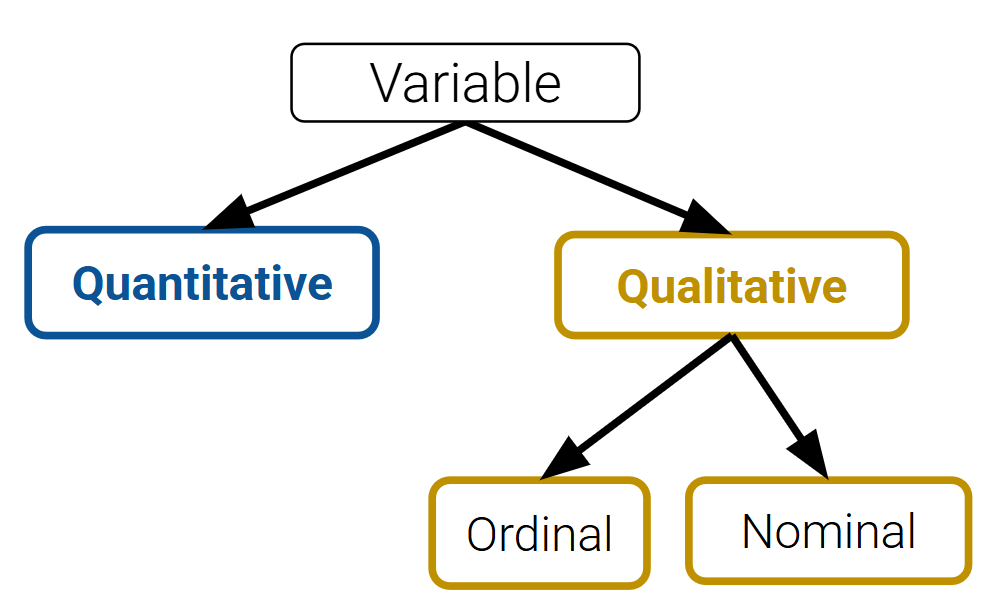
\includegraphics[keepaspectratio]{eda/images/variable_types.png}}

}

\caption{Classification of variable types}

\end{figure}%

Note that many variables don't sit neatly in just one of these
categories. Qualitative variables could have numeric levels, and
conversely, quantitative variables could be stored as strings.

\section{Granularity and Temporality}\label{granularity-and-temporality}

After understanding the structure of the dataset, the next task is to
determine what exactly the data represents. We'll do so by considering
the data's granularity and temporality.

\subsection{Granularity}\label{granularity}

The \textbf{granularity} of a dataset is what a single row represents.
You can also think of it as the level of detail included in the data. To
determine the data's granularity, ask: what does each row in the dataset
represent? Fine-grained data contains a high level of detail, with a
single row representing a small individual unit. For example, each
record may represent one person. Coarse-grained data is encoded such
that a single row represents a large individual unit -- for example,
each record may represent a group of people.

\subsection{Temporality}\label{temporality}

The \textbf{temporality} of a dataset describes the periodicity over
which the data was collected as well as when the data was most recently
collected or updated.

Time and date fields of a dataset could represent a few things:

\begin{enumerate}
\def\labelenumi{\arabic{enumi}.}
\tightlist
\item
  when the ``event'' happened
\item
  when the data was collected, or when it was entered into the system
\item
  when the data was copied into the database
\end{enumerate}

To fully understand the temporality of the data, it also may be
necessary to standardize time zones or inspect recurring time-based
trends in the data (do patterns recur in 24-hour periods? Over the
course of a month? Seasonally?). The convention for standardizing time
is the Coordinated Universal Time (UTC), an international time standard
measured at 0 degrees latitude that stays consistent throughout the year
(no daylight savings). We can represent Berkeley's time zone, Pacific
Standard Time (PST), as UTC-7 (with daylight savings).

\subsubsection{\texorpdfstring{Temporality with \texttt{pandas}'
\texttt{dt}
accessors}{Temporality with pandas' dt accessors}}\label{temporality-with-pandas-dt-accessors}

Let's briefly look at how we can use \texttt{pandas}' \texttt{dt}
accessors to work with dates/times in a dataset using the dataset you'll
see in Lab 3: the Berkeley PD Calls for Service dataset.

\begin{Shaded}
\begin{Highlighting}[]
\NormalTok{calls }\OperatorTok{=}\NormalTok{ pd.read\_csv(}\StringTok{"data/Berkeley\_PD\_{-}\_Calls\_for\_Service.csv"}\NormalTok{)}
\NormalTok{calls.head()}
\end{Highlighting}
\end{Shaded}

\begin{longtable}[]{@{}llllllllllll@{}}
\toprule\noalign{}
& CASENO & OFFENSE & EVENTDT & EVENTTM & CVLEGEND & CVDOW & InDbDate &
Block\_Location & BLKADDR & City & State \\
\midrule\noalign{}
\endhead
\bottomrule\noalign{}
\endlastfoot
0 & 21014296 & THEFT MISD. (UNDER \$950) & 04/01/2021 12:00:00 AM &
10:58 & LARCENY & 4 & 06/15/2021 12:00:00 AM & Berkeley,
CA\textbackslash n(37.869058, -122.270455) & NaN & Berkeley & CA \\
1 & 21014391 & THEFT MISD. (UNDER \$950) & 04/01/2021 12:00:00 AM &
10:38 & LARCENY & 4 & 06/15/2021 12:00:00 AM & Berkeley,
CA\textbackslash n(37.869058, -122.270455) & NaN & Berkeley & CA \\
2 & 21090494 & THEFT MISD. (UNDER \$950) & 04/19/2021 12:00:00 AM &
12:15 & LARCENY & 1 & 06/15/2021 12:00:00 AM & 2100 BLOCK HASTE
ST\textbackslash nBerkeley, CA\textbackslash n(37.864908,... & 2100
BLOCK HASTE ST & Berkeley & CA \\
3 & 21090204 & THEFT FELONY (OVER \$950) & 02/13/2021 12:00:00 AM &
17:00 & LARCENY & 6 & 06/15/2021 12:00:00 AM & 2600 BLOCK WARRING
ST\textbackslash nBerkeley, CA\textbackslash n(37.86393... & 2600 BLOCK
WARRING ST & Berkeley & CA \\
4 & 21090179 & BURGLARY AUTO & 02/08/2021 12:00:00 AM & 6:20 & BURGLARY
- VEHICLE & 1 & 06/15/2021 12:00:00 AM & 2700 BLOCK GARBER
ST\textbackslash nBerkeley, CA\textbackslash n(37.86066,... & 2700 BLOCK
GARBER ST & Berkeley & CA \\
\end{longtable}

Looks like there are three columns with dates/times: \texttt{EVENTDT},
\texttt{EVENTTM}, and \texttt{InDbDate}.

Most likely, \texttt{EVENTDT} stands for the date when the event took
place, \texttt{EVENTTM} stands for the time of day the event took place
(in 24-hr format), and \texttt{InDbDate} is the date this call is
recorded onto the database.

If we check the data type of these columns, we will see they are stored
as strings. We can convert them to \texttt{datetime} objects using
pandas \texttt{to\_datetime} function.

\begin{Shaded}
\begin{Highlighting}[]
\NormalTok{calls[}\StringTok{"EVENTDT"}\NormalTok{] }\OperatorTok{=}\NormalTok{ pd.to\_datetime(calls[}\StringTok{"EVENTDT"}\NormalTok{])}
\NormalTok{calls.head()}
\end{Highlighting}
\end{Shaded}

\begin{longtable}[]{@{}llllllllllll@{}}
\toprule\noalign{}
& CASENO & OFFENSE & EVENTDT & EVENTTM & CVLEGEND & CVDOW & InDbDate &
Block\_Location & BLKADDR & City & State \\
\midrule\noalign{}
\endhead
\bottomrule\noalign{}
\endlastfoot
0 & 21014296 & THEFT MISD. (UNDER \$950) & 2021-04-01 & 10:58 & LARCENY
& 4 & 06/15/2021 12:00:00 AM & Berkeley, CA\textbackslash n(37.869058,
-122.270455) & NaN & Berkeley & CA \\
1 & 21014391 & THEFT MISD. (UNDER \$950) & 2021-04-01 & 10:38 & LARCENY
& 4 & 06/15/2021 12:00:00 AM & Berkeley, CA\textbackslash n(37.869058,
-122.270455) & NaN & Berkeley & CA \\
2 & 21090494 & THEFT MISD. (UNDER \$950) & 2021-04-19 & 12:15 & LARCENY
& 1 & 06/15/2021 12:00:00 AM & 2100 BLOCK HASTE
ST\textbackslash nBerkeley, CA\textbackslash n(37.864908,... & 2100
BLOCK HASTE ST & Berkeley & CA \\
3 & 21090204 & THEFT FELONY (OVER \$950) & 2021-02-13 & 17:00 & LARCENY
& 6 & 06/15/2021 12:00:00 AM & 2600 BLOCK WARRING
ST\textbackslash nBerkeley, CA\textbackslash n(37.86393... & 2600 BLOCK
WARRING ST & Berkeley & CA \\
4 & 21090179 & BURGLARY AUTO & 2021-02-08 & 6:20 & BURGLARY - VEHICLE &
1 & 06/15/2021 12:00:00 AM & 2700 BLOCK GARBER
ST\textbackslash nBerkeley, CA\textbackslash n(37.86066,... & 2700 BLOCK
GARBER ST & Berkeley & CA \\
\end{longtable}

Now, we can use the \texttt{dt} accessor on this column.

We can get the month:

\begin{Shaded}
\begin{Highlighting}[]
\NormalTok{calls[}\StringTok{"EVENTDT"}\NormalTok{].dt.month.head()}
\end{Highlighting}
\end{Shaded}

\begin{verbatim}
0    4
1    4
2    4
3    2
4    2
Name: EVENTDT, dtype: int32
\end{verbatim}

Which day of the week the date is on:

\begin{Shaded}
\begin{Highlighting}[]
\NormalTok{calls[}\StringTok{"EVENTDT"}\NormalTok{].dt.dayofweek.head()}
\end{Highlighting}
\end{Shaded}

\begin{verbatim}
0    3
1    3
2    0
3    5
4    0
Name: EVENTDT, dtype: int32
\end{verbatim}

Check the mimimum values to see if there are any suspicious-looking, 70s
dates:

\begin{Shaded}
\begin{Highlighting}[]
\NormalTok{calls.sort\_values(}\StringTok{"EVENTDT"}\NormalTok{).head()}
\end{Highlighting}
\end{Shaded}

\begin{longtable}[]{@{}llllllllllll@{}}
\toprule\noalign{}
& CASENO & OFFENSE & EVENTDT & EVENTTM & CVLEGEND & CVDOW & InDbDate &
Block\_Location & BLKADDR & City & State \\
\midrule\noalign{}
\endhead
\bottomrule\noalign{}
\endlastfoot
2513 & 20057398 & BURGLARY COMMERCIAL & 2020-12-17 & 16:05 & BURGLARY -
COMMERCIAL & 4 & 06/15/2021 12:00:00 AM & 600 BLOCK GILMAN
ST\textbackslash nBerkeley, CA\textbackslash n(37.878405,... & 600 BLOCK
GILMAN ST & Berkeley & CA \\
624 & 20057207 & ASSAULT/BATTERY MISD. & 2020-12-17 & 16:50 & ASSAULT &
4 & 06/15/2021 12:00:00 AM & 2100 BLOCK SHATTUCK
AVE\textbackslash nBerkeley, CA\textbackslash n(37.871... & 2100 BLOCK
SHATTUCK AVE & Berkeley & CA \\
154 & 20092214 & THEFT FROM AUTO & 2020-12-17 & 18:30 & LARCENY - FROM
VEHICLE & 4 & 06/15/2021 12:00:00 AM & 800 BLOCK SHATTUCK
AVE\textbackslash nBerkeley, CA\textbackslash n(37.8918... & 800 BLOCK
SHATTUCK AVE & Berkeley & CA \\
659 & 20057324 & THEFT MISD. (UNDER \$950) & 2020-12-17 & 15:44 &
LARCENY & 4 & 06/15/2021 12:00:00 AM & 1800 BLOCK 4TH
ST\textbackslash nBerkeley, CA\textbackslash n(37.869888, -... & 1800
BLOCK 4TH ST & Berkeley & CA \\
993 & 20057573 & BURGLARY RESIDENTIAL & 2020-12-17 & 22:15 & BURGLARY -
RESIDENTIAL & 4 & 06/15/2021 12:00:00 AM & 1700 BLOCK STUART
ST\textbackslash nBerkeley, CA\textbackslash n(37.857495... & 1700 BLOCK
STUART ST & Berkeley & CA \\
\end{longtable}

Doesn't look like it! We are good!

We can also do many things with the \texttt{dt} accessor like switching
time zones and converting time back to UNIX/POSIX time. Check out the
documentation on
\href{https://pandas.pydata.org/docs/user_guide/basics.html\#basics-dt-accessors}{\texttt{.dt}
accessor} and
\href{https://pandas.pydata.org/docs/user_guide/timeseries.html\#}{time
series/date functionality}.

\section{Faithfulness}\label{faithfulness}

At this stage in our data cleaning and EDA workflow, we've achieved
quite a lot: we've identified how our data is structured, come to terms
with what information it encodes, and gained insight as to how it was
generated. Throughout this process, we should always recall the original
intent of our work in Data Science -- to use data to better understand
and model the real world. To achieve this goal, we need to ensure that
the data we use is faithful to reality; that is, that our data
accurately captures the ``real world.''

Data used in research or industry is often ``messy'' -- there may be
errors or inaccuracies that impact the faithfulness of the dataset.
Signs that data may not be faithful include:

\begin{itemize}
\tightlist
\item
  Unrealistic or ``incorrect'' values, such as negative counts,
  locations that don't exist, or dates set in the future
\item
  Violations of obvious dependencies, like an age that does not match a
  birthday
\item
  Clear signs that data was entered by hand, which can lead to spelling
  errors or fields that are incorrectly shifted
\item
  Signs of data falsification, such as fake email addresses or repeated
  use of the same names
\item
  Duplicated records or fields containing the same information
\item
  Truncated data, e.g.~Microsoft Excel would limit the number of rows to
  655536 and the number of columns to 255
\end{itemize}

We often solve some of these more common issues in the following ways:

\begin{itemize}
\tightlist
\item
  Spelling errors: apply corrections or drop records that aren't in a
  dictionary
\item
  Time zone inconsistencies: convert to a common time zone (e.g.~UTC)
\item
  Duplicated records or fields: identify and eliminate duplicates (using
  primary keys)
\item
  Unspecified or inconsistent units: infer the units and check that
  values are in reasonable ranges in the data
\end{itemize}

\subsection{Missing Values}\label{missing-values}

Another common issue encountered with real-world datasets is that of
missing data. One strategy to resolve this is to simply drop any records
with missing values from the dataset. This does, however, introduce the
risk of inducing biases -- it is possible that the missing or corrupt
records may be systemically related to some feature of interest in the
data. Another solution is to keep the data as \texttt{NaN} values.

A third method to address missing data is to perform
\textbf{imputation}: infer the missing values using other data available
in the dataset. There is a wide variety of imputation techniques that
can be implemented; some of the most common are listed below.

\begin{itemize}
\tightlist
\item
  Average imputation: replace missing values with the average value for
  that field
\item
  Hot deck imputation: replace missing values with some random value
\item
  Regression imputation: develop a model to predict missing values and
  replace with the predicted value from the model.
\item
  Multiple imputation: replace missing values with multiple random
  values
\end{itemize}

Regardless of the strategy used to deal with missing data, we should
think carefully about \emph{why} particular records or fields may be
missing -- this can help inform whether or not the absence of these
values is significant or meaningful.

\section{EDA Demo 1: Tuberculosis in the United
States}\label{eda-demo-1-tuberculosis-in-the-united-states}

Now, let's walk through the data-cleaning and EDA workflow to see what
can we learn about the presence of Tuberculosis in the United States!

We will examine the data included in the
\href{https://www.cdc.gov/mmwr/volumes/71/wr/mm7112a1.htm?s_cid=mm7112a1_w\#T1_down}{original
CDC article} published in 2021.

\subsection{CSVs and Field Names}\label{csvs-and-field-names}

Suppose Table 1 was saved as a CSV file located in
\texttt{data/cdc\_tuberculosis.csv}.

We can then explore the CSV (which is a text file, and does not contain
binary-encoded data) in many ways: 1. Using a text editor like emacs,
vim, VSCode, etc. 2. Opening the CSV directly in DataHub (read-only),
Excel, Google Sheets, etc. 3. The \texttt{Python} file object 4.
\texttt{pandas}, using \texttt{pd.read\_csv()}

To try out options 1 and 2, you can view or download the Tuberculosis
from the
\href{https://data100.datahub.berkeley.edu/hub/user-redirect/git-pull?repo=https\%3A\%2F\%2Fgithub.com\%2FDS-100\%2Fsp25-student&urlpath=lab\%2Ftree\%2Fsp25-student\%2Flecture\%2Flec05\%2Flec05-part-1-eda-tuberculosis.ipynb&branch=main}{lecture
demo notebook} under the \texttt{data} folder in the left hand menu.
Notice how the CSV file is a type of \textbf{rectangular data (i.e.,
tabular data) stored as comma-separated values}.

Next, let's try out option 3 using the \texttt{Python} file object.
We'll look at the first four lines:

\begin{Shaded}
\begin{Highlighting}[]
\ControlFlowTok{with} \BuiltInTok{open}\NormalTok{(}\StringTok{"data/cdc\_tuberculosis.csv"}\NormalTok{, }\StringTok{"r"}\NormalTok{) }\ImportTok{as}\NormalTok{ f:}
\NormalTok{    i }\OperatorTok{=} \DecValTok{0}
    \ControlFlowTok{for}\NormalTok{ row }\KeywordTok{in}\NormalTok{ f:}
        \BuiltInTok{print}\NormalTok{(row)}
\NormalTok{        i }\OperatorTok{+=} \DecValTok{1}
        \ControlFlowTok{if}\NormalTok{ i }\OperatorTok{\textgreater{}} \DecValTok{3}\NormalTok{:}
            \ControlFlowTok{break}
\end{Highlighting}
\end{Shaded}

\begin{verbatim}
,No. of TB cases,,

U.S. jurisdiction,2019,2020,2021

Total,"8,900","7,173","7,860"

Alabama,87,72,92
\end{verbatim}

Whoa, why are there blank lines interspaced between the lines of the
CSV?

You may recall that all line breaks in text files are encoded as the
special newline character \texttt{\textbackslash{}n}. Python's
\texttt{print()} prints each string (including the newline), and an
additional newline on top of that.

If you're curious, we can use the \texttt{repr()} function to return the
raw string with all special characters:

\begin{Shaded}
\begin{Highlighting}[]
\ControlFlowTok{with} \BuiltInTok{open}\NormalTok{(}\StringTok{"data/cdc\_tuberculosis.csv"}\NormalTok{, }\StringTok{"r"}\NormalTok{) }\ImportTok{as}\NormalTok{ f:}
\NormalTok{    i }\OperatorTok{=} \DecValTok{0}
    \ControlFlowTok{for}\NormalTok{ row }\KeywordTok{in}\NormalTok{ f:}
        \BuiltInTok{print}\NormalTok{(}\BuiltInTok{repr}\NormalTok{(row)) }\CommentTok{\# print raw strings}
\NormalTok{        i }\OperatorTok{+=} \DecValTok{1}
        \ControlFlowTok{if}\NormalTok{ i }\OperatorTok{\textgreater{}} \DecValTok{3}\NormalTok{:}
            \ControlFlowTok{break}
\end{Highlighting}
\end{Shaded}

\begin{verbatim}
',No. of TB cases,,\n'
'U.S. jurisdiction,2019,2020,2021\n'
'Total,"8,900","7,173","7,860"\n'
'Alabama,87,72,92\n'
\end{verbatim}

Finally, let's try option 4 and use the tried-and-true Data 100
approach: \texttt{pandas}.

\begin{Shaded}
\begin{Highlighting}[]
\NormalTok{tb\_df }\OperatorTok{=}\NormalTok{ pd.read\_csv(}\StringTok{"data/cdc\_tuberculosis.csv"}\NormalTok{)}
\NormalTok{tb\_df.head()}
\end{Highlighting}
\end{Shaded}

\begin{longtable}[]{@{}lllll@{}}
\toprule\noalign{}
& Unnamed: 0 & No. of TB cases & Unnamed: 2 & Unnamed: 3 \\
\midrule\noalign{}
\endhead
\bottomrule\noalign{}
\endlastfoot
0 & U.S. jurisdiction & 2019 & 2020 & 2021 \\
1 & Total & 8,900 & 7,173 & 7,860 \\
2 & Alabama & 87 & 72 & 92 \\
3 & Alaska & 58 & 58 & 58 \\
4 & Arizona & 183 & 136 & 129 \\
\end{longtable}

You may notice some strange things about this table: what's up with the
``Unnamed'' column names and the first row?

Congratulations --- you're ready to wrangle your data! Because of how
things are stored, we'll need to clean the data a bit to name our
columns better.

A reasonable first step is to identify the row with the right header.
The \texttt{pd.read\_csv()} function
(\href{https://pandas.pydata.org/docs/reference/api/pandas.read_csv.html}{documentation})
has the convenient \texttt{header} parameter that we can set to use the
elements in row 1 as the appropriate columns:

\begin{Shaded}
\begin{Highlighting}[]
\NormalTok{tb\_df }\OperatorTok{=}\NormalTok{ pd.read\_csv(}\StringTok{"data/cdc\_tuberculosis.csv"}\NormalTok{, header}\OperatorTok{=}\DecValTok{1}\NormalTok{) }\CommentTok{\# row index}
\NormalTok{tb\_df.head(}\DecValTok{5}\NormalTok{)}
\end{Highlighting}
\end{Shaded}

\begin{longtable}[]{@{}lllll@{}}
\toprule\noalign{}
& U.S. jurisdiction & 2019 & 2020 & 2021 \\
\midrule\noalign{}
\endhead
\bottomrule\noalign{}
\endlastfoot
0 & Total & 8,900 & 7,173 & 7,860 \\
1 & Alabama & 87 & 72 & 92 \\
2 & Alaska & 58 & 58 & 58 \\
3 & Arizona & 183 & 136 & 129 \\
4 & Arkansas & 64 & 59 & 69 \\
\end{longtable}

\subsection{Record Granularity}\label{record-granularity}

You might already be wondering: what's up with that first record?

Row 0 is what we call a \textbf{rollup record}, or summary record. It's
often useful when displaying tables to humans. The \textbf{granularity}
of record 0 (Totals) vs the rest of the records (States) is different.

Okay, EDA step two. How was the rollup record aggregated?

Let's check if Total TB cases is the sum of all state TB cases. If we
sum over all rows, we should get \textbf{2x} the total cases in each of
our TB cases by year (why do you think this is?).

\begin{Shaded}
\begin{Highlighting}[]
\NormalTok{tb\_df.}\BuiltInTok{sum}\NormalTok{(axis}\OperatorTok{=}\DecValTok{0}\NormalTok{)}
\end{Highlighting}
\end{Shaded}

\begin{verbatim}
U.S. jurisdiction    TotalAlabamaAlaskaArizonaArkansasCaliforniaCol...
2019                 8,9008758183642,111666718245583029973261085237...
2020                 7,1737258136591,706525417194122219282169239376...
2021                 7,8609258129691,750585443194992281064255127494...
dtype: object
\end{verbatim}

Whoa, what's going on with the TB cases in 2019, 2020, and 2021? Check
out the column types:

\begin{Shaded}
\begin{Highlighting}[]
\NormalTok{tb\_df.dtypes}
\end{Highlighting}
\end{Shaded}

\begin{verbatim}
U.S. jurisdiction    object
2019                 object
2020                 object
2021                 object
dtype: object
\end{verbatim}

Since there are commas in the values for TB cases, the numbers are read
as the \texttt{object} datatype, or \textbf{storage type} (close to the
\texttt{Python} string datatype), so \texttt{pandas} is concatenating
strings instead of adding integers (recall that Python can ``sum'', or
concatenate, strings together: \texttt{"data"\ +\ "100"} evaluates to
\texttt{"data100"}).

Fortunately \texttt{read\_csv} also has a \texttt{thousands} parameter
(\href{https://pandas.pydata.org/docs/reference/api/pandas.read_csv.html}{documentation}):

\begin{Shaded}
\begin{Highlighting}[]
\CommentTok{\# improve readability: chaining method calls with outer parentheses/line breaks}
\NormalTok{tb\_df }\OperatorTok{=}\NormalTok{ (}
\NormalTok{    pd.read\_csv(}\StringTok{"data/cdc\_tuberculosis.csv"}\NormalTok{, header}\OperatorTok{=}\DecValTok{1}\NormalTok{, thousands}\OperatorTok{=}\StringTok{\textquotesingle{},\textquotesingle{}}\NormalTok{)}
\NormalTok{)}
\NormalTok{tb\_df.head(}\DecValTok{5}\NormalTok{)}
\end{Highlighting}
\end{Shaded}

\begin{longtable}[]{@{}lllll@{}}
\toprule\noalign{}
& U.S. jurisdiction & 2019 & 2020 & 2021 \\
\midrule\noalign{}
\endhead
\bottomrule\noalign{}
\endlastfoot
0 & Total & 8900 & 7173 & 7860 \\
1 & Alabama & 87 & 72 & 92 \\
2 & Alaska & 58 & 58 & 58 \\
3 & Arizona & 183 & 136 & 129 \\
4 & Arkansas & 64 & 59 & 69 \\
\end{longtable}

\begin{Shaded}
\begin{Highlighting}[]
\NormalTok{tb\_df.}\BuiltInTok{sum}\NormalTok{()}
\end{Highlighting}
\end{Shaded}

\begin{verbatim}
U.S. jurisdiction    TotalAlabamaAlaskaArizonaArkansasCaliforniaCol...
2019                                                             17800
2020                                                             14346
2021                                                             15720
dtype: object
\end{verbatim}

The total TB cases look right. Phew!

Let's just look at the records with \textbf{state-level granularity}:

\begin{Shaded}
\begin{Highlighting}[]
\NormalTok{state\_tb\_df }\OperatorTok{=}\NormalTok{ tb\_df[}\DecValTok{1}\NormalTok{:]}
\NormalTok{state\_tb\_df.head(}\DecValTok{5}\NormalTok{)}
\end{Highlighting}
\end{Shaded}

\begin{longtable}[]{@{}lllll@{}}
\toprule\noalign{}
& U.S. jurisdiction & 2019 & 2020 & 2021 \\
\midrule\noalign{}
\endhead
\bottomrule\noalign{}
\endlastfoot
1 & Alabama & 87 & 72 & 92 \\
2 & Alaska & 58 & 58 & 58 \\
3 & Arizona & 183 & 136 & 129 \\
4 & Arkansas & 64 & 59 & 69 \\
5 & California & 2111 & 1706 & 1750 \\
\end{longtable}

\subsection{Gather Census Data}\label{gather-census-data}

U.S. Census population estimates
\href{https://www.census.gov/data/tables/time-series/demo/popest/2010s-state-total.html}{source}
(2019),
\href{https://www.census.gov/data/tables/time-series/demo/popest/2020s-state-total.html}{source}
(2020-2024).

Running the below cells cleans the data. There are a few new methods
here:

\begin{itemize}
\tightlist
\item
  \texttt{df.convert\_dtypes()}
  (\href{https://pandas.pydata.org/docs/reference/api/pandas.DataFrame.convert_dtypes.html}{documentation})
  conveniently converts all float dtypes into ints and is out of scope
  for the class.
\item
  \texttt{df.drop\_na()}
  (\href{https://pandas.pydata.org/docs/reference/api/pandas.DataFrame.dropna.html}{documentation})
  will be explained in more detail next time.
\end{itemize}

\begin{Shaded}
\begin{Highlighting}[]
\CommentTok{\# 2010s census data}
\NormalTok{census\_2010s\_df }\OperatorTok{=}\NormalTok{ pd.read\_csv(}\StringTok{"data/nst{-}est2019{-}01.csv"}\NormalTok{, header}\OperatorTok{=}\DecValTok{3}\NormalTok{, thousands}\OperatorTok{=}\StringTok{","}\NormalTok{)}
\NormalTok{census\_2010s\_df }\OperatorTok{=}\NormalTok{ (}
\NormalTok{    census\_2010s\_df}
\NormalTok{    .rename(columns}\OperatorTok{=}\NormalTok{\{}\StringTok{"Unnamed: 0"}\NormalTok{: }\StringTok{"Geographic Area"}\NormalTok{\})}
\NormalTok{    .drop(columns}\OperatorTok{=}\NormalTok{[}\StringTok{"Census"}\NormalTok{, }\StringTok{"Estimates Base"}\NormalTok{])}
\NormalTok{    .convert\_dtypes() }\CommentTok{\# "smart" converting of columns to int, use at your own risk}
\NormalTok{    .dropna()  }\CommentTok{\# we\textquotesingle{}ll introduce this very soon}
\NormalTok{)}
\NormalTok{census\_2010s\_df[}\StringTok{\textquotesingle{}Geographic Area\textquotesingle{}}\NormalTok{] }\OperatorTok{=}\NormalTok{ census\_2010s\_df[}\StringTok{\textquotesingle{}Geographic Area\textquotesingle{}}\NormalTok{].}\BuiltInTok{str}\NormalTok{.strip(}\StringTok{\textquotesingle{}.\textquotesingle{}}\NormalTok{)}

\CommentTok{\# with pd.option\_context(\textquotesingle{}display.min\_rows\textquotesingle{}, 30): \# shows more rows}
\CommentTok{\#     display(census\_2010s\_df)}
    
\NormalTok{census\_2010s\_df.head(}\DecValTok{5}\NormalTok{)}
\end{Highlighting}
\end{Shaded}

\begin{longtable}[]{@{}llllllllllll@{}}
\toprule\noalign{}
& Geographic Area & 2010 & 2011 & 2012 & 2013 & 2014 & 2015 & 2016 &
2017 & 2018 & 2019 \\
\midrule\noalign{}
\endhead
\bottomrule\noalign{}
\endlastfoot
0 & United States & 309321666 & 311556874 & 313830990 & 315993715 &
318301008 & 320635163 & 322941311 & 324985539 & 326687501 & 328239523 \\
1 & Northeast & 55380134 & 55604223 & 55775216 & 55901806 & 56006011 &
56034684 & 56042330 & 56059240 & 56046620 & 55982803 \\
2 & Midwest & 66974416 & 67157800 & 67336743 & 67560379 & 67745167 &
67860583 & 67987540 & 68126781 & 68236628 & 68329004 \\
3 & South & 114866680 & 116006522 & 117241208 & 118364400 & 119624037 &
120997341 & 122351760 & 123542189 & 124569433 & 125580448 \\
4 & West & 72100436 & 72788329 & 73477823 & 74167130 & 74925793 &
75742555 & 76559681 & 77257329 & 77834820 & 78347268 \\
\end{longtable}

Occasionally, you will want to modify code that you have imported. To
reimport those modifications you can either use \texttt{python}'s
\texttt{importlib} library:

\begin{Shaded}
\begin{Highlighting}[]
\ImportTok{from}\NormalTok{ importlib }\ImportTok{import} \BuiltInTok{reload}
\BuiltInTok{reload}\NormalTok{(utils)}
\end{Highlighting}
\end{Shaded}

or use \texttt{iPython} magic which will intelligently import code when
files change:

\begin{Shaded}
\begin{Highlighting}[]
\OperatorTok{\%}\NormalTok{load\_ext autoreload}
\OperatorTok{\%}\NormalTok{autoreload }\DecValTok{2}
\end{Highlighting}
\end{Shaded}

\begin{Shaded}
\begin{Highlighting}[]
\CommentTok{\# census 2020s data}
\NormalTok{census\_2020s\_df }\OperatorTok{=}\NormalTok{ pd.read\_csv(}\StringTok{"data/NST{-}EST2024{-}POP.csv"}\NormalTok{, header}\OperatorTok{=}\DecValTok{3}\NormalTok{, thousands}\OperatorTok{=}\StringTok{","}\NormalTok{)}
\NormalTok{census\_2020s\_df }\OperatorTok{=}\NormalTok{ (}
\NormalTok{    census\_2020s\_df}
\NormalTok{    .drop(columns}\OperatorTok{=}\NormalTok{[}\StringTok{"Unnamed: 1"}\NormalTok{])}
\NormalTok{    .rename(columns}\OperatorTok{=}\NormalTok{\{}\StringTok{"Unnamed: 0"}\NormalTok{: }\StringTok{"Geographic Area"}\NormalTok{\})}
\NormalTok{    .loc[:, }\StringTok{"Geographic Area"}\NormalTok{:}\StringTok{"2024"}\NormalTok{] }\CommentTok{\# ignore all the blank extra columns}
\NormalTok{    .convert\_dtypes()                 }\CommentTok{\# "smart" converting of columns, use at your own risk}
\NormalTok{    .dropna()                         }\CommentTok{\# we\textquotesingle{}ll introduce this next ti}
\NormalTok{)}
\NormalTok{census\_2020s\_df[}\StringTok{\textquotesingle{}Geographic Area\textquotesingle{}}\NormalTok{] }\OperatorTok{=}\NormalTok{ census\_2020s\_df[}\StringTok{\textquotesingle{}Geographic Area\textquotesingle{}}\NormalTok{].}\BuiltInTok{str}\NormalTok{.strip(}\StringTok{\textquotesingle{}.\textquotesingle{}}\NormalTok{)}

\NormalTok{census\_2020s\_df.head(}\DecValTok{5}\NormalTok{)}
\end{Highlighting}
\end{Shaded}

\begin{longtable}[]{@{}lllllll@{}}
\toprule\noalign{}
& Geographic Area & 2020 & 2021 & 2022 & 2023 & 2024 \\
\midrule\noalign{}
\endhead
\bottomrule\noalign{}
\endlastfoot
0 & United States & 331577720 & 332099760 & 334017321 & 336806231 &
340110988 \\
1 & Northeast & 57431458 & 57252533 & 57159597 & 57398303 & 57832935 \\
2 & Midwest & 68984258 & 68872831 & 68903297 & 69186401 & 69596584 \\
3 & South & 126476549 & 127368010 & 129037849 & 130893358 & 132665693 \\
4 & West & 78685455 & 78606386 & 78916578 & 79328169 & 80015776 \\
\end{longtable}

\subsection{\texorpdfstring{Joining Data (Merging
\texttt{DataFrame}s)}{Joining Data (Merging DataFrames)}}\label{joining-data-merging-dataframes}

Time to \texttt{merge}! Here we use the \texttt{DataFrame} method
\texttt{df1.merge(right=df2,\ ...)} on \texttt{DataFrame} \texttt{df1}
(\href{https://pandas.pydata.org/docs/reference/api/pandas.DataFrame.merge.html}{documentation}).
Contrast this with the function
\texttt{pd.merge(left=df1,\ right=df2,\ ...)}
(\href{https://pandas.pydata.org/docs/reference/api/pandas.merge.html?highlight=pandas\%20merge\#pandas.merge}{documentation}).
Feel free to use either.

\begin{Shaded}
\begin{Highlighting}[]
\CommentTok{\# merge TB DataFrame with two US census DataFrames}
\NormalTok{tb\_census\_df }\OperatorTok{=}\NormalTok{ (}
\NormalTok{    tb\_df}
\NormalTok{    .merge(right}\OperatorTok{=}\NormalTok{census\_2010s\_df,}
\NormalTok{           left\_on}\OperatorTok{=}\StringTok{"U.S. jurisdiction"}\NormalTok{, right\_on}\OperatorTok{=}\StringTok{"Geographic Area"}\NormalTok{)}
\NormalTok{    .merge(right}\OperatorTok{=}\NormalTok{census\_2020s\_df,}
\NormalTok{           left\_on}\OperatorTok{=}\StringTok{"U.S. jurisdiction"}\NormalTok{, right\_on}\OperatorTok{=}\StringTok{"Geographic Area"}\NormalTok{)}
\NormalTok{)}
\NormalTok{tb\_census\_df.head(}\DecValTok{5}\NormalTok{)}
\end{Highlighting}
\end{Shaded}

\begin{longtable}[]{@{}llllllllllllllllllllll@{}}
\toprule\noalign{}
& U.S. jurisdiction & 2019\_x & 2020\_x & 2021\_x & Geographic Area\_x &
2010 & 2011 & 2012 & 2013 & 2014 & 2015 & 2016 & 2017 & 2018 & 2019\_y &
Geographic Area\_y & 2020\_y & 2021\_y & 2022 & 2023 & 2024 \\
\midrule\noalign{}
\endhead
\bottomrule\noalign{}
\endlastfoot
0 & Alabama & 87 & 72 & 92 & Alabama & 4785437 & 4799069 & 4815588 &
4830081 & 4841799 & 4852347 & 4863525 & 4874486 & 4887681 & 4903185 &
Alabama & 5033094 & 5049196 & 5076181 & 5117673 & 5157699 \\
1 & Alaska & 58 & 58 & 58 & Alaska & 713910 & 722128 & 730443 & 737068 &
736283 & 737498 & 741456 & 739700 & 735139 & 731545 & Alaska & 733017 &
734420 & 734442 & 736510 & 740133 \\
2 & Arizona & 183 & 136 & 129 & Arizona & 6407172 & 6472643 & 6554978 &
6632764 & 6730413 & 6829676 & 6941072 & 7044008 & 7158024 & 7278717 &
Arizona & 7187135 & 7274078 & 7377566 & 7473027 & 7582384 \\
3 & Arkansas & 64 & 59 & 69 & Arkansas & 2921964 & 2940667 & 2952164 &
2959400 & 2967392 & 2978048 & 2989918 & 3001345 & 3009733 & 3017804 &
Arkansas & 3014546 & 3026870 & 3047704 & 3069463 & 3088354 \\
4 & California & 2111 & 1706 & 1750 & California & 37319502 & 37638369 &
37948800 & 38260787 & 38596972 & 38918045 & 39167117 & 39358497 &
39461588 & 39512223 & California & 39521958 & 39142565 & 39142414 &
39198693 & 39431263 \\
\end{longtable}

We're only interested in the population for the years 2019, 2020, and
2021, so let's select just those columns:

\begin{Shaded}
\begin{Highlighting}[]
\NormalTok{census\_2019\_df }\OperatorTok{=}\NormalTok{ census\_2010s\_df[[}\StringTok{\textquotesingle{}Geographic Area\textquotesingle{}}\NormalTok{, }\StringTok{\textquotesingle{}2019\textquotesingle{}}\NormalTok{]]}
\NormalTok{census\_2020\_2021\_df }\OperatorTok{=}\NormalTok{ census\_2020s\_df[[}\StringTok{\textquotesingle{}Geographic Area\textquotesingle{}}\NormalTok{, }\StringTok{\textquotesingle{}2020\textquotesingle{}}\NormalTok{, }\StringTok{\textquotesingle{}2021\textquotesingle{}}\NormalTok{]]}

\NormalTok{display(tb\_df.tail(}\DecValTok{2}\NormalTok{))}
\NormalTok{display(census\_2019\_df.tail(}\DecValTok{2}\NormalTok{))}
\NormalTok{display(census\_2020\_2021\_df.tail(}\DecValTok{2}\NormalTok{))}
\end{Highlighting}
\end{Shaded}

\begin{longtable}[]{@{}lllll@{}}
\toprule\noalign{}
& U.S. jurisdiction & 2019 & 2020 & 2021 \\
\midrule\noalign{}
\endhead
\bottomrule\noalign{}
\endlastfoot
50 & Wisconsin & 51 & 35 & 66 \\
51 & Wyoming & 1 & 0 & 3 \\
\end{longtable}

\begin{longtable}[]{@{}lll@{}}
\toprule\noalign{}
& Geographic Area & 2019 \\
\midrule\noalign{}
\endhead
\bottomrule\noalign{}
\endlastfoot
55 & Wyoming & 578759 \\
57 & Puerto Rico & 3193694 \\
\end{longtable}

\begin{longtable}[]{@{}llll@{}}
\toprule\noalign{}
& Geographic Area & 2020 & 2021 \\
\midrule\noalign{}
\endhead
\bottomrule\noalign{}
\endlastfoot
55 & Wyoming & 577681 & 579636 \\
57 & Puerto Rico & 3281590 & 3262711 \\
\end{longtable}

All three dataframes have a column containing U.S. states, along with
some other geographic areas. These columns are our \textbf{join keys}.

\begin{itemize}
\item
  Below, we use \texttt{df1.merge(right=df2,\ ...)} to carry out the
  merge
  (\href{https://pandas.pydata.org/docs/reference/api/pandas.DataFrame.merge.html}{documentation}).
\item
  We could have alternatively used the function
  \texttt{pd.merge(left=df1,\ right=df2,\ ...)}
  (\href{https://pandas.pydata.org/docs/reference/api/pandas.merge.html\#pandas.merge}{documentation}).
\end{itemize}

\begin{Shaded}
\begin{Highlighting}[]
\CommentTok{\# merge TB dataframe with two US census dataframes}
\NormalTok{tb\_census\_df }\OperatorTok{=}\NormalTok{ (}
\NormalTok{    tb\_df}
\NormalTok{    .merge(right}\OperatorTok{=}\NormalTok{census\_2019\_df,}
\NormalTok{           left\_on}\OperatorTok{=}\StringTok{"U.S. jurisdiction"}\NormalTok{, right\_on}\OperatorTok{=}\StringTok{"Geographic Area"}\NormalTok{)}
\NormalTok{    .merge(right}\OperatorTok{=}\NormalTok{census\_2020\_2021\_df,}
\NormalTok{           left\_on}\OperatorTok{=}\StringTok{"U.S. jurisdiction"}\NormalTok{, right\_on}\OperatorTok{=}\StringTok{"Geographic Area"}\NormalTok{)}
\NormalTok{)}
\NormalTok{tb\_census\_df.tail(}\DecValTok{2}\NormalTok{)}
\end{Highlighting}
\end{Shaded}

\begin{longtable}[]{@{}llllllllll@{}}
\toprule\noalign{}
& U.S. jurisdiction & 2019\_x & 2020\_x & 2021\_x & Geographic Area\_x &
2019\_y & Geographic Area\_y & 2020\_y & 2021\_y \\
\midrule\noalign{}
\endhead
\bottomrule\noalign{}
\endlastfoot
49 & Wisconsin & 51 & 35 & 66 & Wisconsin & 5822434 & Wisconsin &
5897375 & 5881608 \\
50 & Wyoming & 1 & 0 & 3 & Wyoming & 578759 & Wyoming & 577681 &
579636 \\
\end{longtable}

To see what's going on with the duplicate columns, and the \texttt{\_x}
and \texttt{\_y}, let's do the just the first merge:

\begin{Shaded}
\begin{Highlighting}[]
\NormalTok{tb\_df.merge(right}\OperatorTok{=}\NormalTok{census\_2019\_df, }
\NormalTok{            left\_on}\OperatorTok{=}\StringTok{"U.S. jurisdiction"}\NormalTok{, }
\NormalTok{            right\_on}\OperatorTok{=}\StringTok{"Geographic Area"}\NormalTok{).head()}
\end{Highlighting}
\end{Shaded}

\begin{longtable}[]{@{}lllllll@{}}
\toprule\noalign{}
& U.S. jurisdiction & 2019\_x & 2020 & 2021 & Geographic Area &
2019\_y \\
\midrule\noalign{}
\endhead
\bottomrule\noalign{}
\endlastfoot
0 & Alabama & 87 & 72 & 92 & Alabama & 4903185 \\
1 & Alaska & 58 & 58 & 58 & Alaska & 731545 \\
2 & Arizona & 183 & 136 & 129 & Arizona & 7278717 \\
3 & Arkansas & 64 & 59 & 69 & Arkansas & 3017804 \\
4 & California & 2111 & 1706 & 1750 & California & 39512223 \\
\end{longtable}

Notice that the columns containing the \textbf{join keys} have all been
retained, and all contain the same values.

\begin{itemize}
\item
  Furthermore, notice that the duplicated columns are appended with
  \texttt{\_x} and \texttt{\_y} to keep the column names unique.
\item
  In the TB case count data, column \texttt{2019} represents the number
  of TB cases in 2019, but in the Census data, column \texttt{2019}
  represents the U.S. population.
\end{itemize}

We can use the \texttt{suffixes} argument to modify the \texttt{\_x} and
\texttt{\_y} defaults to our liking
(\href{https://pandas.pydata.org/docs/reference/api/pandas.merge.html\#pandas.merge}{documentation}).

\begin{Shaded}
\begin{Highlighting}[]
\CommentTok{\# Specify the suffixes to use for duplicated column names}
\NormalTok{tb\_df.merge(right}\OperatorTok{=}\NormalTok{census\_2019\_df,}
\NormalTok{           left\_on}\OperatorTok{=}\StringTok{"U.S. jurisdiction"}\NormalTok{, }
\NormalTok{           right\_on}\OperatorTok{=}\StringTok{"Geographic Area"}\NormalTok{,}
\NormalTok{           suffixes}\OperatorTok{=}\NormalTok{(}\StringTok{\textquotesingle{}\_cases\textquotesingle{}}\NormalTok{, }\StringTok{\textquotesingle{}\_population\textquotesingle{}}\NormalTok{)).head()}
\end{Highlighting}
\end{Shaded}

\begin{longtable}[]{@{}lllllll@{}}
\toprule\noalign{}
& U.S. jurisdiction & 2019\_cases & 2020 & 2021 & Geographic Area &
2019\_population \\
\midrule\noalign{}
\endhead
\bottomrule\noalign{}
\endlastfoot
0 & Alabama & 87 & 72 & 92 & Alabama & 4903185 \\
1 & Alaska & 58 & 58 & 58 & Alaska & 731545 \\
2 & Arizona & 183 & 136 & 129 & Arizona & 7278717 \\
3 & Arkansas & 64 & 59 & 69 & Arkansas & 3017804 \\
4 & California & 2111 & 1706 & 1750 & California & 39512223 \\
\end{longtable}

Notice the \texttt{\_x} and \texttt{\_y} have changed to
\texttt{\_cases} and \texttt{\_population}, just like we specified.

Putting it all together, and dropping the duplicated
\texttt{Geographic\ Area} columns:

\begin{Shaded}
\begin{Highlighting}[]
\CommentTok{\# Redux: merge TB dataframe with two US census dataframes}
\NormalTok{tb\_census\_df }\OperatorTok{=}\NormalTok{ (}
\NormalTok{    tb\_df}
    
\NormalTok{    .merge(right}\OperatorTok{=}\NormalTok{census\_2019\_df,}
\NormalTok{           left\_on}\OperatorTok{=}\StringTok{"U.S. jurisdiction"}\NormalTok{, right\_on}\OperatorTok{=}\StringTok{"Geographic Area"}\NormalTok{,}
\NormalTok{           suffixes}\OperatorTok{=}\NormalTok{(}\StringTok{\textquotesingle{}\_cases\textquotesingle{}}\NormalTok{, }\StringTok{\textquotesingle{}\_population\textquotesingle{}}\NormalTok{))}
\NormalTok{    .drop(columns}\OperatorTok{=}\StringTok{"Geographic Area"}\NormalTok{)}

\NormalTok{    .merge(right}\OperatorTok{=}\NormalTok{census\_2020\_2021\_df,}
\NormalTok{           left\_on}\OperatorTok{=}\StringTok{"U.S. jurisdiction"}\NormalTok{, right\_on}\OperatorTok{=}\StringTok{"Geographic Area"}\NormalTok{,}
\NormalTok{           suffixes}\OperatorTok{=}\NormalTok{(}\StringTok{\textquotesingle{}\_cases\textquotesingle{}}\NormalTok{, }\StringTok{\textquotesingle{}\_population\textquotesingle{}}\NormalTok{))}
\NormalTok{    .drop(columns}\OperatorTok{=}\StringTok{"Geographic Area"}\NormalTok{)}
    
\NormalTok{)}
\NormalTok{tb\_census\_df.tail(}\DecValTok{2}\NormalTok{)}
\end{Highlighting}
\end{Shaded}

\begin{longtable}[]{@{}llllllll@{}}
\toprule\noalign{}
& U.S. jurisdiction & 2019\_cases & 2020\_cases & 2021\_cases &
2019\_population & 2020\_population & 2021\_population \\
\midrule\noalign{}
\endhead
\bottomrule\noalign{}
\endlastfoot
49 & Wisconsin & 51 & 35 & 66 & 5822434 & 5897375 & 5881608 \\
50 & Wyoming & 1 & 0 & 3 & 578759 & 577681 & 579636 \\
\end{longtable}

\subsection{Reproducing Data: Compute
Incidence}\label{reproducing-data-compute-incidence}

Let's see if we can reproduce the original CDC numbers from our
augmented dataset of TB case counts and state populations.

\begin{itemize}
\item
  Recall that the nationwide TB incidence was \textbf{2.7 in 2019},
  \textbf{2.2 in 2020}, and \textbf{2.4 in 2021}.
\item
  Along the way, we'll also compute state-level incidence.
\end{itemize}

From the
\href{https://www.cdc.gov/mmwr/volumes/71/wr/mm7112a1.htm?s_cid=mm7112a1_w\#T1_down}{CDC
report}: TB incidence is computed as ``Cases per 100,000 persons using
mid-year population estimates from the U.S. Census Bureau.''

Let's start with a simpler question: What is the per person incidence?

\begin{itemize}
\tightlist
\item
  In other words, what is the probability that a randomly selected
  person in the population had TB within a given year?
\end{itemize}

\[\text{TB incidence per person} = \frac{\text{\# TB cases in population}}{\text{Total population size}}\]

Let's calculate per person incidence for 2019:

\begin{Shaded}
\begin{Highlighting}[]
\CommentTok{\# Calculate per person incidence for 2019}
\NormalTok{tb\_census\_df[}\StringTok{"per person incidence 2019"}\NormalTok{] }\OperatorTok{=}\NormalTok{ (}
\NormalTok{    tb\_census\_df[}\StringTok{"2019\_cases"}\NormalTok{]}\OperatorTok{/}\NormalTok{tb\_census\_df[}\StringTok{"2019\_population"}\NormalTok{]}
\NormalTok{)}
\NormalTok{tb\_census\_df}
\end{Highlighting}
\end{Shaded}

\begin{longtable}[]{@{}lllllllll@{}}
\toprule\noalign{}
& U.S. jurisdiction & 2019\_cases & 2020\_cases & 2021\_cases &
2019\_population & 2020\_population & 2021\_population & per person
incidence 2019 \\
\midrule\noalign{}
\endhead
\bottomrule\noalign{}
\endlastfoot
0 & Alabama & 87 & 72 & 92 & 4903185 & 5033094 & 5049196 & 0.00 \\
1 & Alaska & 58 & 58 & 58 & 731545 & 733017 & 734420 & 0.00 \\
2 & Arizona & 183 & 136 & 129 & 7278717 & 7187135 & 7274078 & 0.00 \\
3 & Arkansas & 64 & 59 & 69 & 3017804 & 3014546 & 3026870 & 0.00 \\
4 & California & 2111 & 1706 & 1750 & 39512223 & 39521958 & 39142565 &
0.00 \\
... & ... & ... & ... & ... & ... & ... & ... & ... \\
46 & Virginia & 191 & 169 & 161 & 8535519 & 8637615 & 8658910 & 0.00 \\
47 & Washington & 221 & 163 & 199 & 7614893 & 7727209 & 7743760 &
0.00 \\
48 & West Virginia & 9 & 13 & 7 & 1792147 & 1791646 & 1785618 & 0.00 \\
49 & Wisconsin & 51 & 35 & 66 & 5822434 & 5897375 & 5881608 & 0.00 \\
50 & Wyoming & 1 & 0 & 3 & 578759 & 577681 & 579636 & 0.00 \\
\end{longtable}

TB is really rare in the United States, so per person TB incidence is
really low, as expected.

\begin{itemize}
\item
  But, if we were to consider 100,000 people, the probability of seeing
  a TB case is higher.
\item
  In fact, it would be 100,000 times higher!
\end{itemize}

\[\text{TB incidence per 100,000} = \text{100,000} * \text{TB incidence per person}\]

\begin{Shaded}
\begin{Highlighting}[]
\CommentTok{\# To help read bigger numbers in Python, you can use \_ to separate thousands,}
\CommentTok{\# akin to using commas. 100\_000 is the same as writing 100000, but more readable.}
\NormalTok{tb\_census\_df[}\StringTok{"per 100k incidence 2019"}\NormalTok{] }\OperatorTok{=}\NormalTok{ (}
    \DecValTok{100\_000} \OperatorTok{*}\NormalTok{ tb\_census\_df[}\StringTok{"per person incidence 2019"}\NormalTok{] }
\NormalTok{)}
\NormalTok{tb\_census\_df}
\end{Highlighting}
\end{Shaded}

\begin{longtable}[]{@{}llllllllll@{}}
\toprule\noalign{}
& U.S. jurisdiction & 2019\_cases & 2020\_cases & 2021\_cases &
2019\_population & 2020\_population & 2021\_population & per person
incidence 2019 & per 100k incidence 2019 \\
\midrule\noalign{}
\endhead
\bottomrule\noalign{}
\endlastfoot
0 & Alabama & 87 & 72 & 92 & 4903185 & 5033094 & 5049196 & 0.00 &
1.77 \\
1 & Alaska & 58 & 58 & 58 & 731545 & 733017 & 734420 & 0.00 & 7.93 \\
2 & Arizona & 183 & 136 & 129 & 7278717 & 7187135 & 7274078 & 0.00 &
2.51 \\
3 & Arkansas & 64 & 59 & 69 & 3017804 & 3014546 & 3026870 & 0.00 &
2.12 \\
4 & California & 2111 & 1706 & 1750 & 39512223 & 39521958 & 39142565 &
0.00 & 5.34 \\
... & ... & ... & ... & ... & ... & ... & ... & ... & ... \\
46 & Virginia & 191 & 169 & 161 & 8535519 & 8637615 & 8658910 & 0.00 &
2.24 \\
47 & Washington & 221 & 163 & 199 & 7614893 & 7727209 & 7743760 & 0.00 &
2.90 \\
48 & West Virginia & 9 & 13 & 7 & 1792147 & 1791646 & 1785618 & 0.00 &
0.50 \\
49 & Wisconsin & 51 & 35 & 66 & 5822434 & 5897375 & 5881608 & 0.00 &
0.88 \\
50 & Wyoming & 1 & 0 & 3 & 578759 & 577681 & 579636 & 0.00 & 0.17 \\
\end{longtable}

Now we're seeing more human-readable values.

\begin{itemize}
\tightlist
\item
  For example, there 5.3 tuberculosis cases for every 100,000 California
  residents in 2019.
\end{itemize}

To wrap up this exercise, let's calculate the nationwide incidence of TB
in 2019.

\begin{Shaded}
\begin{Highlighting}[]
\CommentTok{\# Recall that the CDC reported an incidence of 2.7 per 100,000 in 2019.}
\NormalTok{tot\_tb\_cases\_50\_states }\OperatorTok{=}\NormalTok{ tb\_census\_df[}\StringTok{"2019\_cases"}\NormalTok{].}\BuiltInTok{sum}\NormalTok{()}
\NormalTok{tot\_pop\_50\_states }\OperatorTok{=}\NormalTok{ tb\_census\_df[}\StringTok{"2019\_population"}\NormalTok{].}\BuiltInTok{sum}\NormalTok{()}
\NormalTok{tb\_per\_100k\_50\_states }\OperatorTok{=} \DecValTok{100\_000} \OperatorTok{*}\NormalTok{ tot\_tb\_cases\_50\_states }\OperatorTok{/}\NormalTok{ tot\_pop\_50\_states}
\NormalTok{tb\_per\_100k\_50\_states}
\end{Highlighting}
\end{Shaded}

\begin{verbatim}
np.float64(2.7114346007625656)
\end{verbatim}

We can use a \texttt{for} loop to compute the incidence for 2019, 2020,
and 2021.

\begin{itemize}
\tightlist
\item
  You'll notice that we get the same numbers reported by the CDC!
\end{itemize}

\begin{Shaded}
\begin{Highlighting}[]
\CommentTok{\# f strings (f"...") are a handy way to pass in variables to strings.}
\ControlFlowTok{for}\NormalTok{ year }\KeywordTok{in}\NormalTok{ [}\DecValTok{2019}\NormalTok{, }\DecValTok{2020}\NormalTok{, }\DecValTok{2021}\NormalTok{]:}
\NormalTok{  tot\_tb\_cases\_50\_states }\OperatorTok{=}\NormalTok{ tb\_census\_df[}\SpecialStringTok{f"}\SpecialCharTok{\{}\NormalTok{year}\SpecialCharTok{\}}\SpecialStringTok{\_cases"}\NormalTok{].}\BuiltInTok{sum}\NormalTok{()}
\NormalTok{  tot\_pop\_50\_states }\OperatorTok{=}\NormalTok{ tb\_census\_df[}\SpecialStringTok{f"}\SpecialCharTok{\{}\NormalTok{year}\SpecialCharTok{\}}\SpecialStringTok{\_population"}\NormalTok{].}\BuiltInTok{sum}\NormalTok{()}
\NormalTok{  tb\_per\_100k\_50\_states }\OperatorTok{=} \DecValTok{100\_000} \OperatorTok{*}\NormalTok{ tot\_tb\_cases\_50\_states }\OperatorTok{/}\NormalTok{ tot\_pop\_50\_states}
  \BuiltInTok{print}\NormalTok{(tb\_per\_100k\_50\_states)}
\end{Highlighting}
\end{Shaded}

\begin{verbatim}
2.7114346007625656
2.163293721906285
2.366758711298075
\end{verbatim}

\section{EDA Demo 2: Mauna Loa CO2 Data -- A Lesson in Data
Faithfulness}\label{eda-demo-2-mauna-loa-co2-data-a-lesson-in-data-faithfulness}

\href{https://gml.noaa.gov/ccgg/trends/data.html}{Mauna Loa Observatory}
has been monitoring CO2 concentrations since 1958.

\begin{Shaded}
\begin{Highlighting}[]
\NormalTok{co2\_file }\OperatorTok{=} \StringTok{"data/co2\_mm\_mlo.txt"}
\end{Highlighting}
\end{Shaded}

Let's do some \textbf{EDA}!!

\subsection{\texorpdfstring{Reading this file into
\texttt{Pandas}?}{Reading this file into Pandas?}}\label{reading-this-file-into-pandas}

Let's instead check out this \texttt{.txt} file. Some questions to keep
in mind: Do we trust this file extension? What structure is it?

Lines 71-78 (inclusive) are shown below:

\begin{verbatim}
line number |                            file contents

71          |   #            decimal     average   interpolated    trend    #days
72          |   #             date                             (season corr)
73          |   1958   3    1958.208      315.71      315.71      314.62     -1
74          |   1958   4    1958.292      317.45      317.45      315.29     -1
75          |   1958   5    1958.375      317.50      317.50      314.71     -1
76          |   1958   6    1958.458      -99.99      317.10      314.85     -1
77          |   1958   7    1958.542      315.86      315.86      314.98     -1
78          |   1958   8    1958.625      314.93      314.93      315.94     -1
\end{verbatim}

Notice how:

\begin{itemize}
\tightlist
\item
  The values are separated by white space, possibly tabs.
\item
  The data line up down the rows. For example, the month appears in 7th
  to 8th position of each line.
\item
  The 71st and 72nd lines in the file contain column headings split over
  two lines.
\end{itemize}

We can use~\texttt{read\_csv}~to read the data into a \texttt{pandas}
\texttt{DataFrame}, and we provide several arguments to specify that the
separators are white space, there is no header (\textbf{we will set our
own column names}), and to skip the first 72 rows of the file.

\begin{Shaded}
\begin{Highlighting}[]
\NormalTok{co2 }\OperatorTok{=}\NormalTok{ pd.read\_csv(}
\NormalTok{    co2\_file, header }\OperatorTok{=} \VariableTok{None}\NormalTok{, skiprows }\OperatorTok{=} \DecValTok{72}\NormalTok{,}
\NormalTok{    sep }\OperatorTok{=} \VerbatimStringTok{r\textquotesingle{}\textbackslash{}s+\textquotesingle{}}       \CommentTok{\#delimiter for continuous whitespace (stay tuned for regex next lecture))}
\NormalTok{)}
\NormalTok{co2.head()}
\end{Highlighting}
\end{Shaded}

\begin{longtable}[]{@{}llllllll@{}}
\toprule\noalign{}
& 0 & 1 & 2 & 3 & 4 & 5 & 6 \\
\midrule\noalign{}
\endhead
\bottomrule\noalign{}
\endlastfoot
0 & 1958 & 3 & 1958.21 & 315.71 & 315.71 & 314.62 & -1 \\
1 & 1958 & 4 & 1958.29 & 317.45 & 317.45 & 315.29 & -1 \\
2 & 1958 & 5 & 1958.38 & 317.50 & 317.50 & 314.71 & -1 \\
3 & 1958 & 6 & 1958.46 & -99.99 & 317.10 & 314.85 & -1 \\
4 & 1958 & 7 & 1958.54 & 315.86 & 315.86 & 314.98 & -1 \\
\end{longtable}

Congratulations! You've wrangled the data!

\ldots But our columns aren't named. \textbf{We need to do more EDA.}

\subsection{Exploring Variable Feature
Types}\label{exploring-variable-feature-types}

The NOAA \href{https://gml.noaa.gov/ccgg/trends/}{webpage} might have
some useful tidbits (in this case it doesn't).

Using this information, we'll rerun \texttt{pd.read\_csv}, but this time
with some \textbf{custom column names.}

\begin{Shaded}
\begin{Highlighting}[]
\NormalTok{co2 }\OperatorTok{=}\NormalTok{ pd.read\_csv(}
\NormalTok{    co2\_file, header }\OperatorTok{=} \VariableTok{None}\NormalTok{, skiprows }\OperatorTok{=} \DecValTok{72}\NormalTok{,}
\NormalTok{    sep }\OperatorTok{=} \VerbatimStringTok{r\textquotesingle{}\textbackslash{}s+\textquotesingle{}}\NormalTok{, }\CommentTok{\#regex for continuous whitespace (next lecture)}
\NormalTok{    names }\OperatorTok{=}\NormalTok{ [}\StringTok{\textquotesingle{}Yr\textquotesingle{}}\NormalTok{, }\StringTok{\textquotesingle{}Mo\textquotesingle{}}\NormalTok{, }\StringTok{\textquotesingle{}DecDate\textquotesingle{}}\NormalTok{, }\StringTok{\textquotesingle{}Avg\textquotesingle{}}\NormalTok{, }\StringTok{\textquotesingle{}Int\textquotesingle{}}\NormalTok{, }\StringTok{\textquotesingle{}Trend\textquotesingle{}}\NormalTok{, }\StringTok{\textquotesingle{}Days\textquotesingle{}}\NormalTok{]}
\NormalTok{)}
\NormalTok{co2.head()}
\end{Highlighting}
\end{Shaded}

\begin{longtable}[]{@{}llllllll@{}}
\toprule\noalign{}
& Yr & Mo & DecDate & Avg & Int & Trend & Days \\
\midrule\noalign{}
\endhead
\bottomrule\noalign{}
\endlastfoot
0 & 1958 & 3 & 1958.21 & 315.71 & 315.71 & 314.62 & -1 \\
1 & 1958 & 4 & 1958.29 & 317.45 & 317.45 & 315.29 & -1 \\
2 & 1958 & 5 & 1958.38 & 317.50 & 317.50 & 314.71 & -1 \\
3 & 1958 & 6 & 1958.46 & -99.99 & 317.10 & 314.85 & -1 \\
4 & 1958 & 7 & 1958.54 & 315.86 & 315.86 & 314.98 & -1 \\
\end{longtable}

\subsection{Visualizing CO2}\label{visualizing-co2}

Scientific studies tend to have very clean data, right\ldots? Let's jump
right in and make a time series plot of CO2 monthly averages.

\begin{Shaded}
\begin{Highlighting}[]
\NormalTok{sns.lineplot(x}\OperatorTok{=}\StringTok{\textquotesingle{}DecDate\textquotesingle{}}\NormalTok{, y}\OperatorTok{=}\StringTok{\textquotesingle{}Avg\textquotesingle{}}\NormalTok{, data}\OperatorTok{=}\NormalTok{co2)}\OperatorTok{;}
\end{Highlighting}
\end{Shaded}

\pandocbounded{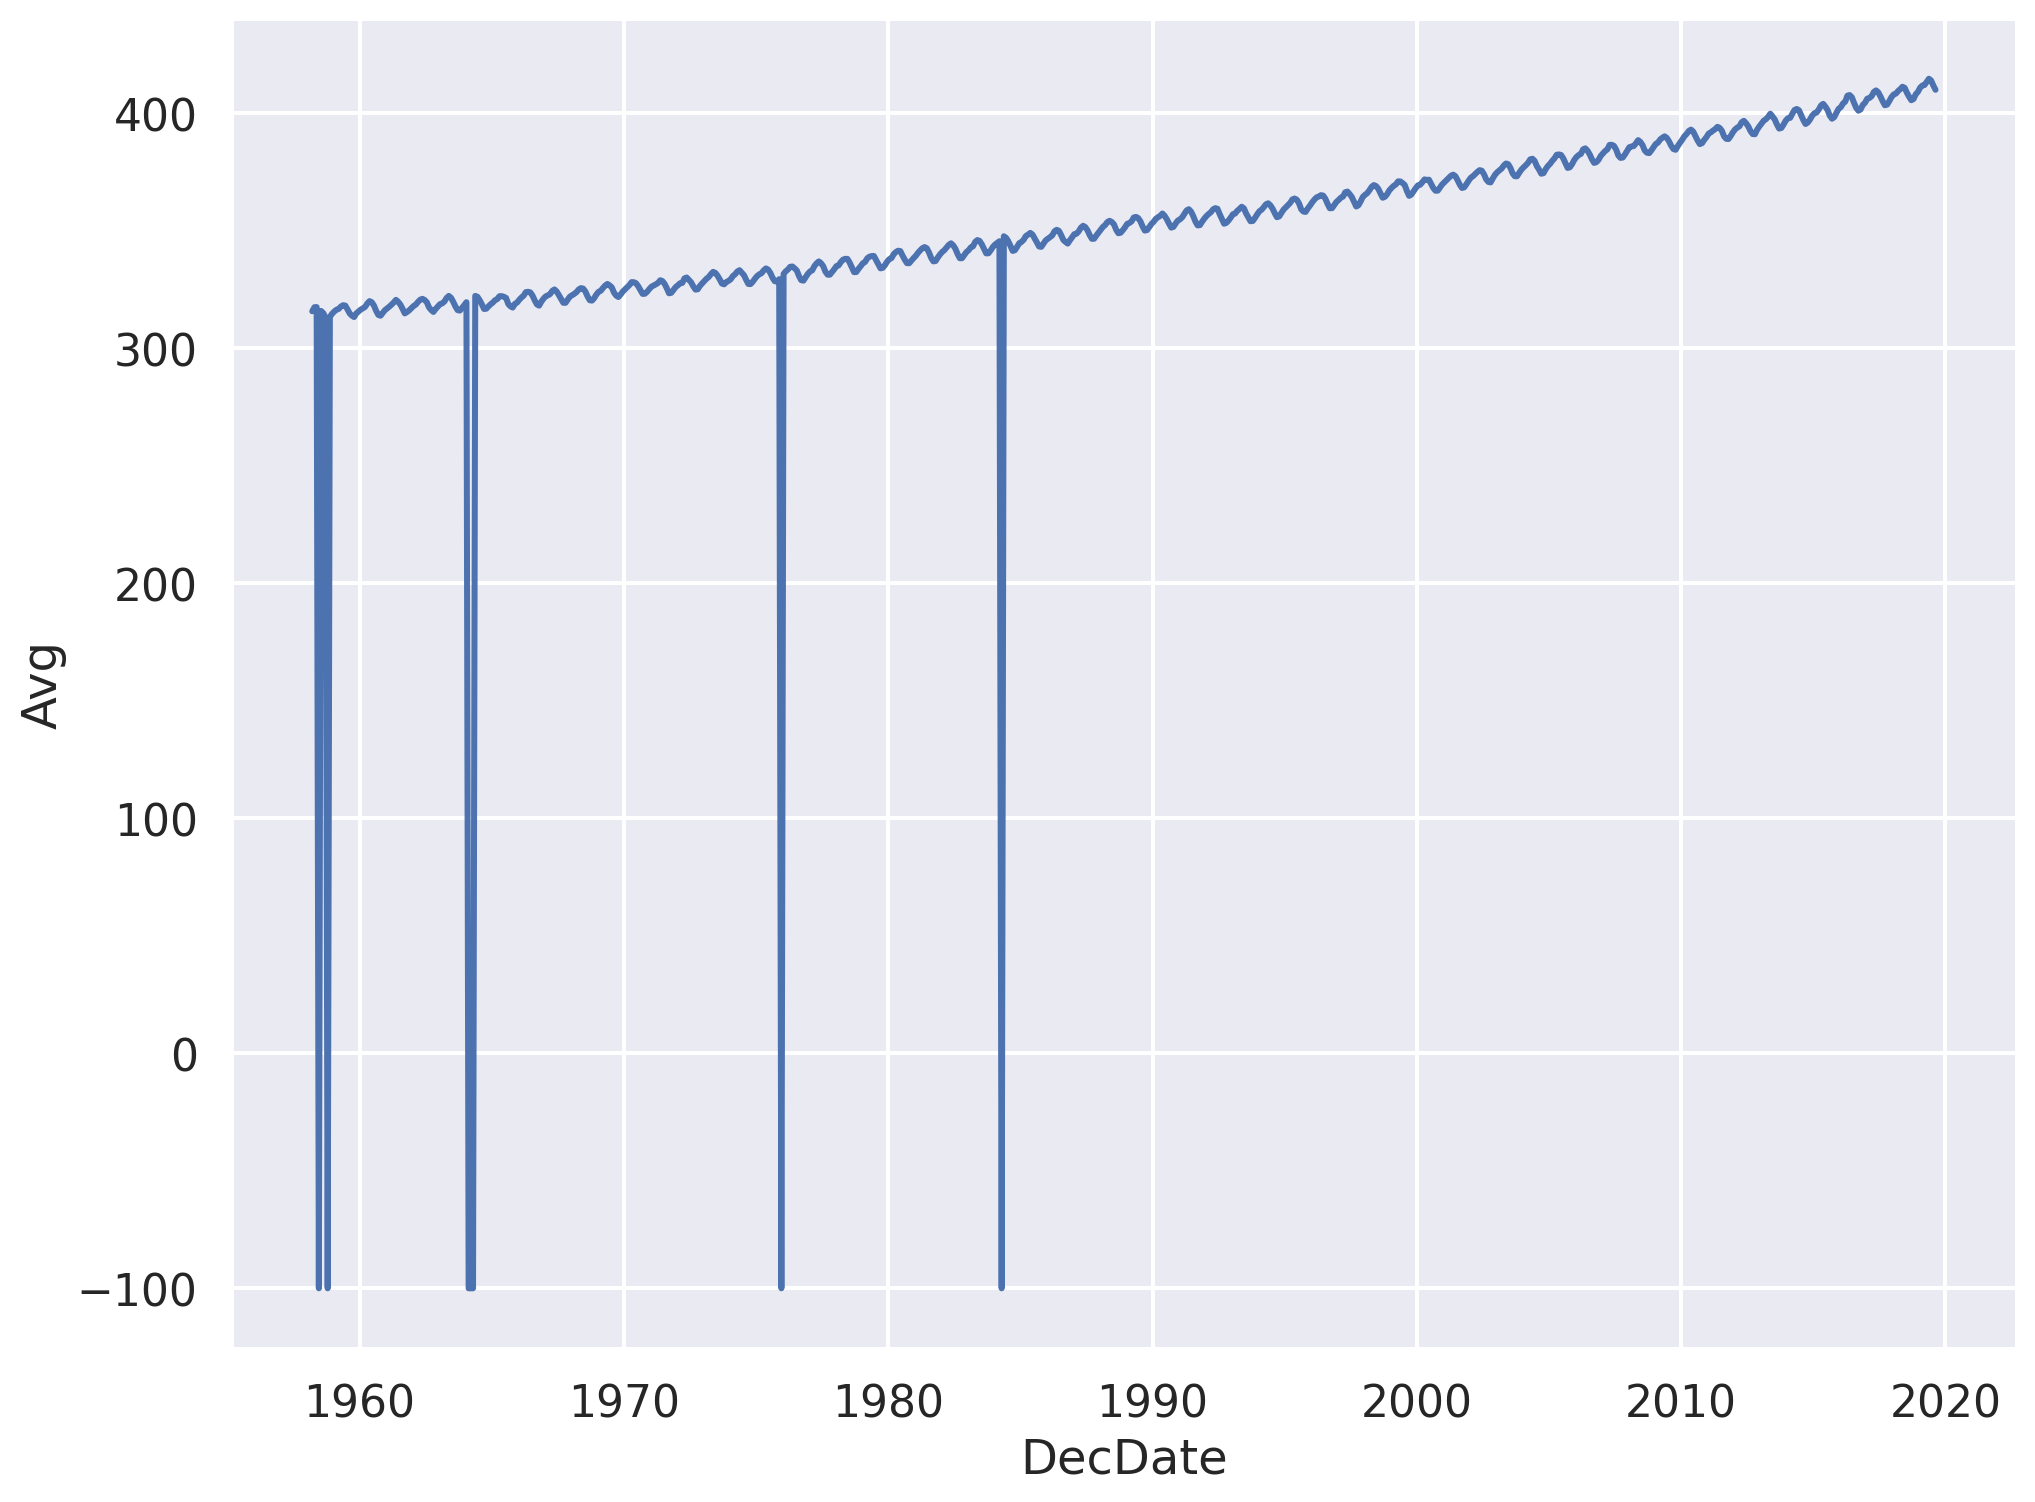
\includegraphics[keepaspectratio]{eda/eda_files/figure-pdf/cell-52-output-1.pdf}}

The code above uses the \texttt{seaborn} plotting library (abbreviated
\texttt{sns}). We will cover this in the Visualization lecture, but now
you don't need to worry about how it works!

Yikes! Plotting the data uncovered a problem. The sharp vertical lines
suggest that we have some \textbf{missing values}. What happened here?

\begin{Shaded}
\begin{Highlighting}[]
\NormalTok{co2.head()}
\end{Highlighting}
\end{Shaded}

\begin{longtable}[]{@{}llllllll@{}}
\toprule\noalign{}
& Yr & Mo & DecDate & Avg & Int & Trend & Days \\
\midrule\noalign{}
\endhead
\bottomrule\noalign{}
\endlastfoot
0 & 1958 & 3 & 1958.21 & 315.71 & 315.71 & 314.62 & -1 \\
1 & 1958 & 4 & 1958.29 & 317.45 & 317.45 & 315.29 & -1 \\
2 & 1958 & 5 & 1958.38 & 317.50 & 317.50 & 314.71 & -1 \\
3 & 1958 & 6 & 1958.46 & -99.99 & 317.10 & 314.85 & -1 \\
4 & 1958 & 7 & 1958.54 & 315.86 & 315.86 & 314.98 & -1 \\
\end{longtable}

\begin{Shaded}
\begin{Highlighting}[]
\NormalTok{co2.tail()}
\end{Highlighting}
\end{Shaded}

\begin{longtable}[]{@{}llllllll@{}}
\toprule\noalign{}
& Yr & Mo & DecDate & Avg & Int & Trend & Days \\
\midrule\noalign{}
\endhead
\bottomrule\noalign{}
\endlastfoot
733 & 2019 & 4 & 2019.29 & 413.32 & 413.32 & 410.49 & 26 \\
734 & 2019 & 5 & 2019.38 & 414.66 & 414.66 & 411.20 & 28 \\
735 & 2019 & 6 & 2019.46 & 413.92 & 413.92 & 411.58 & 27 \\
736 & 2019 & 7 & 2019.54 & 411.77 & 411.77 & 411.43 & 23 \\
737 & 2019 & 8 & 2019.62 & 409.95 & 409.95 & 411.84 & 29 \\
\end{longtable}

Some data have unusual values like -1 and -99.99.

Let's check the description at the top of the file again.

\begin{itemize}
\tightlist
\item
  -1 signifies a missing value for the number of days \texttt{Days} the
  equipment was in operation that month.
\item
  -99.99 denotes a missing monthly average \texttt{Avg}
\end{itemize}

How can we fix this? First, let's explore other aspects of our data.
Understanding our data will help us decide what to do with the missing
values.

\subsection{Sanity Checks: Reasoning about the
data}\label{sanity-checks-reasoning-about-the-data}

First, we consider the shape of the data. How many rows should we have?

\begin{itemize}
\tightlist
\item
  If chronological order, we should have one record per month.
\item
  Data from March 1958 to August 2019.
\item
  We should have \$ 12 \times (2019-1957) - 2 - 4 = 738 \$ records.
\end{itemize}

\begin{Shaded}
\begin{Highlighting}[]
\NormalTok{co2.shape}
\end{Highlighting}
\end{Shaded}

\begin{verbatim}
(738, 7)
\end{verbatim}

Nice!! The number of rows (i.e.~records) match our expectations.

Let's now check the quality of each feature.

\subsection{\texorpdfstring{Understanding Missing Value 1:
\texttt{Days}}{Understanding Missing Value 1: Days}}\label{understanding-missing-value-1-days}

\texttt{Days} is a time field, so let's analyze other time fields to see
if there is an explanation for missing values of days of operation.

Let's start with \textbf{months}, \texttt{Mo}.

Are we missing any records? The number of months should have 62 or 61
instances (March 1957-August 2019).

\begin{Shaded}
\begin{Highlighting}[]
\NormalTok{co2[}\StringTok{"Mo"}\NormalTok{].value\_counts().sort\_index()}
\end{Highlighting}
\end{Shaded}

\begin{verbatim}
Mo
1     61
2     61
3     62
4     62
5     62
6     62
7     62
8     62
9     61
10    61
11    61
12    61
Name: count, dtype: int64
\end{verbatim}

As expected Jan, Feb, Sep, Oct, Nov, and Dec have 61 occurrences and the
rest 62.

Next let's explore \textbf{days} \texttt{Days} itself, which is the
number of days that the measurement equipment worked.

\begin{Shaded}
\begin{Highlighting}[]
\NormalTok{sns.displot(co2[}\StringTok{\textquotesingle{}Days\textquotesingle{}}\NormalTok{])}\OperatorTok{;}
\NormalTok{plt.title(}\StringTok{"Distribution of days feature"}\NormalTok{)}\OperatorTok{;} \CommentTok{\# suppresses unneeded plotting output}
\end{Highlighting}
\end{Shaded}

\pandocbounded{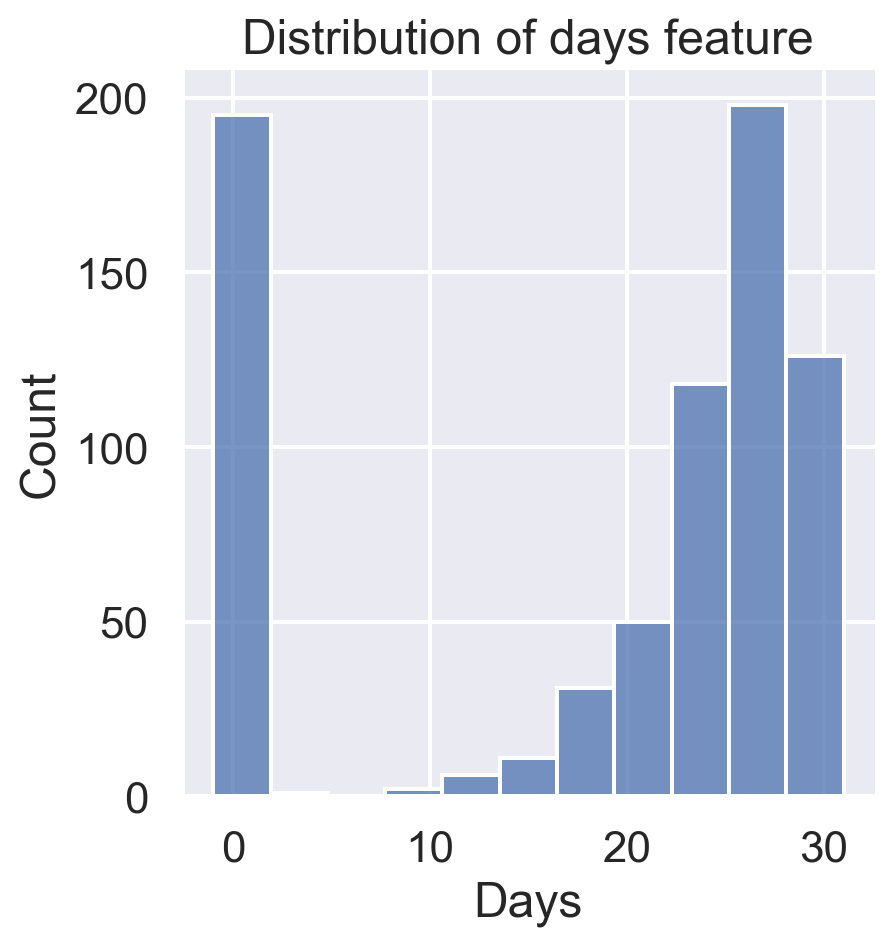
\includegraphics[keepaspectratio]{eda/eda_files/figure-pdf/cell-57-output-1.pdf}}

In terms of data quality, a handful of months have averages based on
measurements taken on fewer than half the days. In addition, there are
nearly 200 missing values--\textbf{that's about 27\% of the data}!

Finally, let's check the last time feature, \textbf{year} \texttt{Yr}.

Let's check to see if there is any connection between missing-ness and
the year of the recording.

\begin{Shaded}
\begin{Highlighting}[]
\NormalTok{sns.scatterplot(x}\OperatorTok{=}\StringTok{"Yr"}\NormalTok{, y}\OperatorTok{=}\StringTok{"Days"}\NormalTok{, data}\OperatorTok{=}\NormalTok{co2)}\OperatorTok{;}
\NormalTok{plt.title(}\StringTok{"Day field by Year"}\NormalTok{)}\OperatorTok{;} \CommentTok{\# the ; suppresses output}
\end{Highlighting}
\end{Shaded}

\pandocbounded{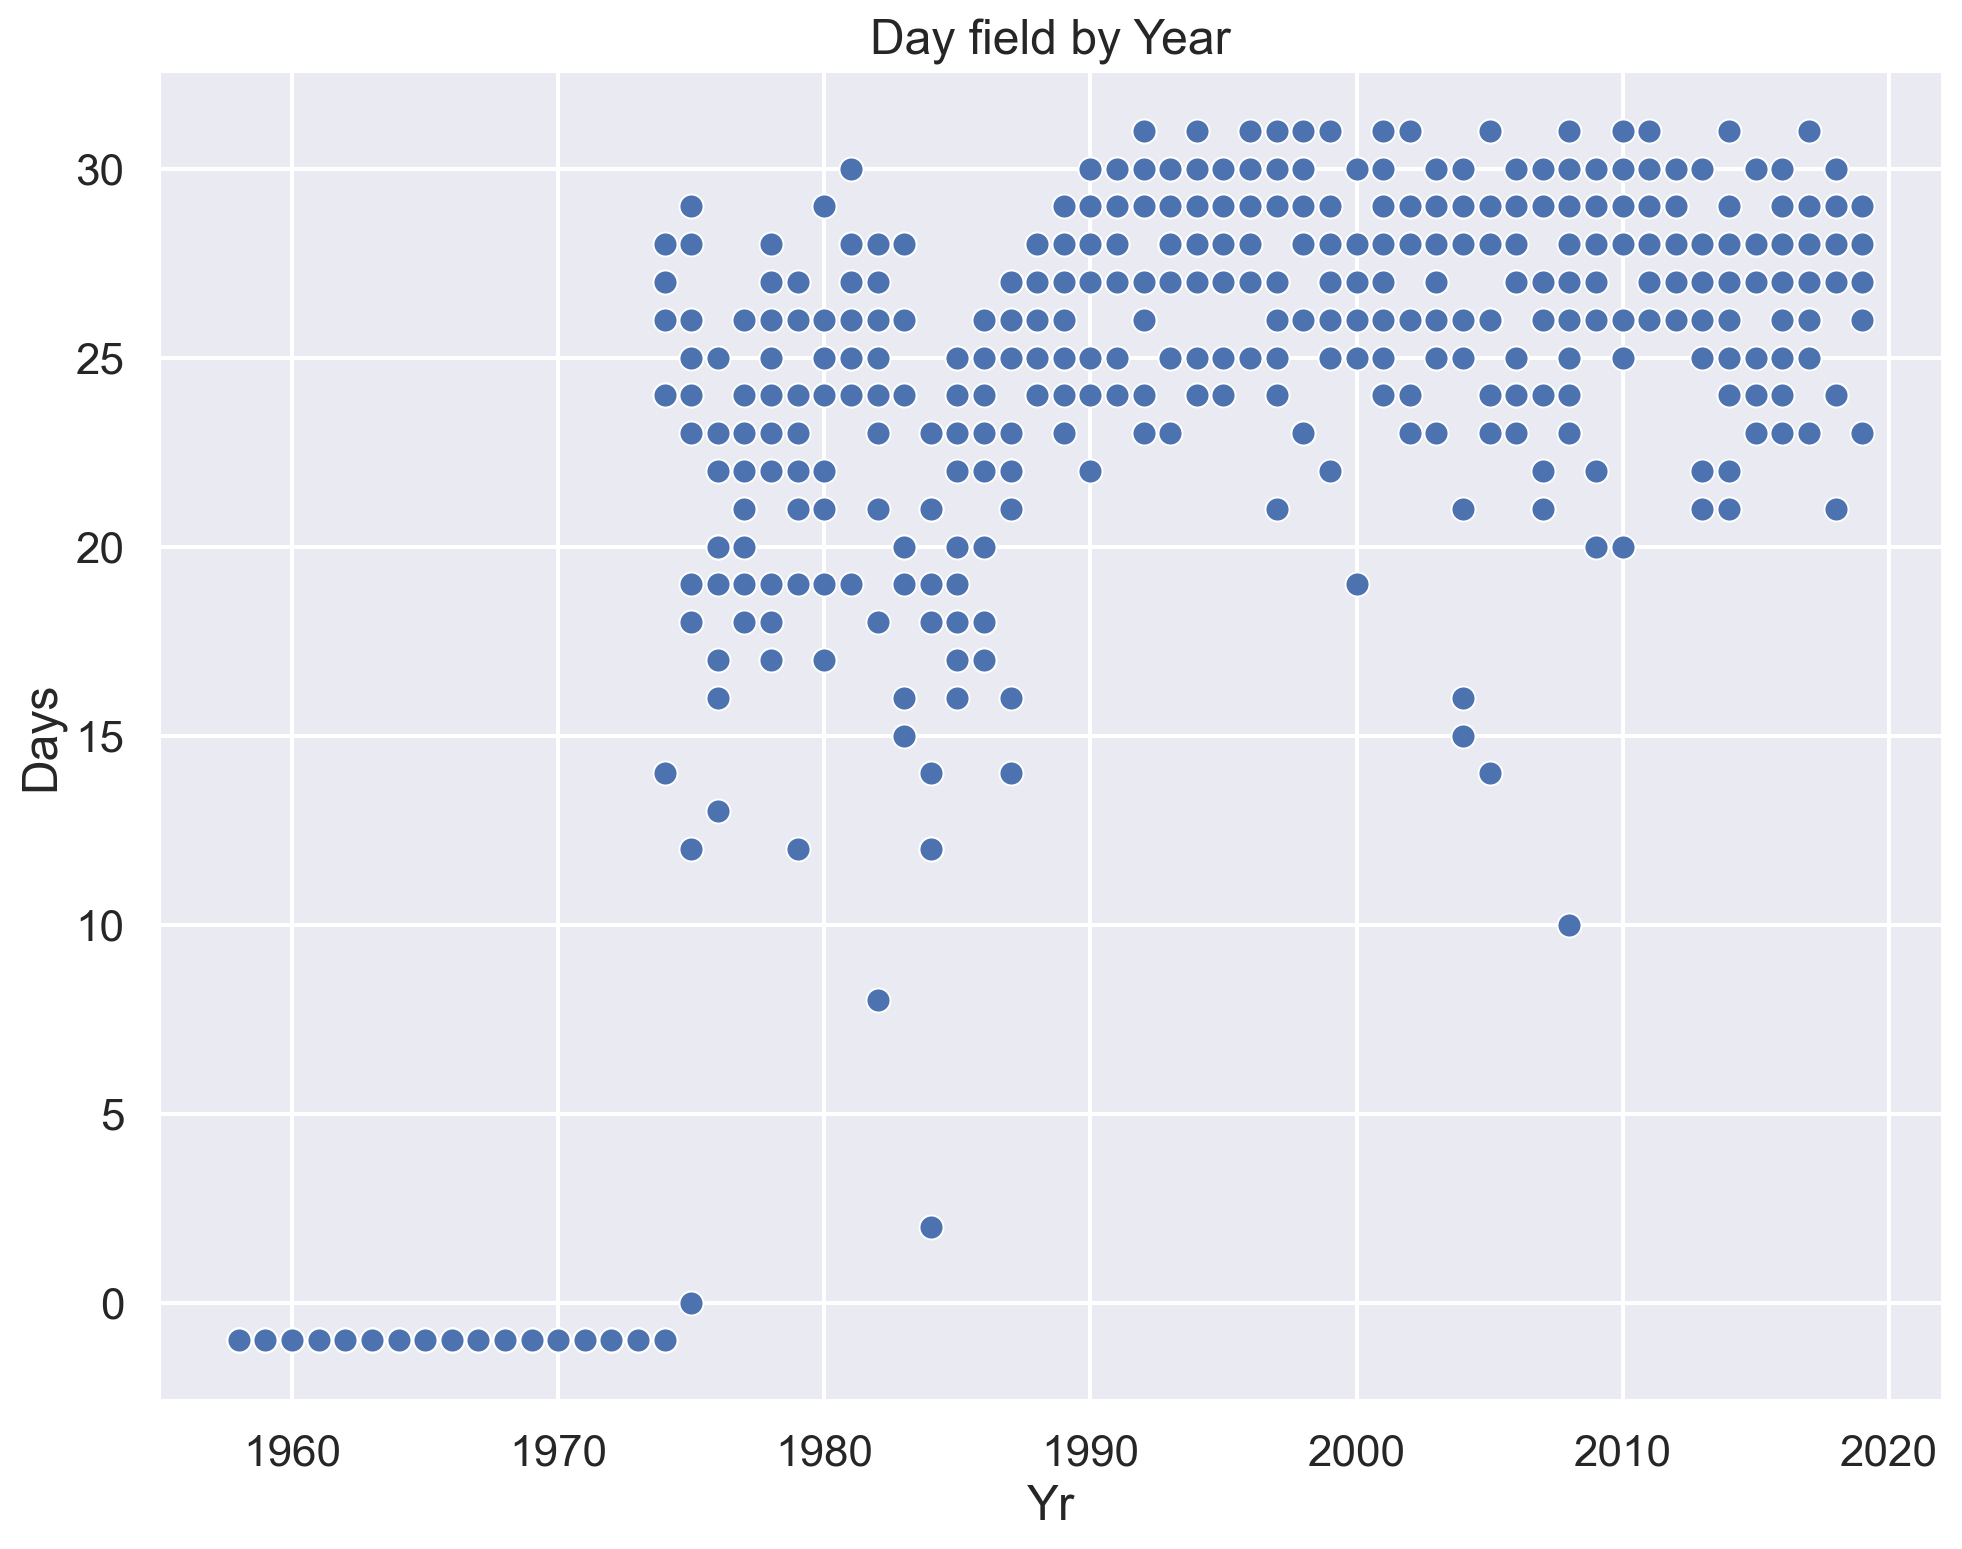
\includegraphics[keepaspectratio]{eda/eda_files/figure-pdf/cell-58-output-1.pdf}}

\textbf{Observations}:

\begin{itemize}
\tightlist
\item
  All of the missing data are in the early years of operation.
\item
  It appears there may have been problems with equipment in the mid to
  late 80s.
\end{itemize}

\textbf{Potential Next Steps}:

\begin{itemize}
\tightlist
\item
  Confirm these explanations through documentation about the historical
  readings.
\item
  Maybe drop the earliest recordings? However, we would want to delay
  such action until after we have examined the time trends and assess
  whether there are any potential problems.
\end{itemize}

\subsection{\texorpdfstring{Understanding Missing Value 2:
\texttt{Avg}}{Understanding Missing Value 2: Avg}}\label{understanding-missing-value-2-avg}

Next, let's return to the -99.99 values in \texttt{Avg} to analyze the
overall quality of the CO2 measurements. We'll plot a histogram of the
average CO2 measurements

\begin{Shaded}
\begin{Highlighting}[]
\CommentTok{\# Histograms of average CO2 measurements}
\NormalTok{sns.displot(co2[}\StringTok{\textquotesingle{}Avg\textquotesingle{}}\NormalTok{])}\OperatorTok{;}
\end{Highlighting}
\end{Shaded}

\pandocbounded{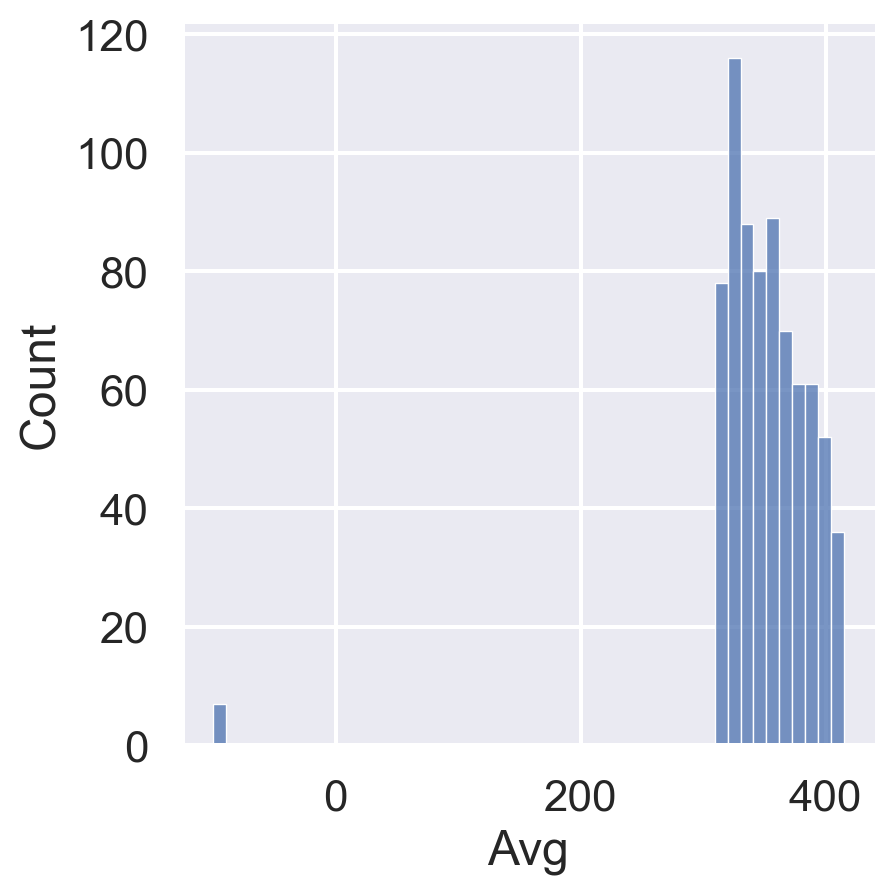
\includegraphics[keepaspectratio]{eda/eda_files/figure-pdf/cell-59-output-1.pdf}}

The non-missing values are in the 300-400 range (a regular range of CO2
levels).

We also see that there are only a few missing \texttt{Avg} values
(\textbf{\textless1\% of values}). Let's examine all of them:

\begin{Shaded}
\begin{Highlighting}[]
\NormalTok{co2[co2[}\StringTok{"Avg"}\NormalTok{] }\OperatorTok{\textless{}} \DecValTok{0}\NormalTok{]}
\end{Highlighting}
\end{Shaded}

\begin{longtable}[]{@{}llllllll@{}}
\toprule\noalign{}
& Yr & Mo & DecDate & Avg & Int & Trend & Days \\
\midrule\noalign{}
\endhead
\bottomrule\noalign{}
\endlastfoot
3 & 1958 & 6 & 1958.46 & -99.99 & 317.10 & 314.85 & -1 \\
7 & 1958 & 10 & 1958.79 & -99.99 & 312.66 & 315.61 & -1 \\
71 & 1964 & 2 & 1964.12 & -99.99 & 320.07 & 319.61 & -1 \\
72 & 1964 & 3 & 1964.21 & -99.99 & 320.73 & 319.55 & -1 \\
73 & 1964 & 4 & 1964.29 & -99.99 & 321.77 & 319.48 & -1 \\
213 & 1975 & 12 & 1975.96 & -99.99 & 330.59 & 331.60 & 0 \\
313 & 1984 & 4 & 1984.29 & -99.99 & 346.84 & 344.27 & 2 \\
\end{longtable}

There doesn't seem to be a pattern to these values, other than that most
records also were missing \texttt{Days} data.

\subsection{\texorpdfstring{Drop, \texttt{NaN}, or Impute Missing
\texttt{Avg}
Data?}{Drop, NaN, or Impute Missing Avg Data?}}\label{drop-nan-or-impute-missing-avg-data}

How should we address the invalid \texttt{Avg} data?

\begin{enumerate}
\def\labelenumi{\arabic{enumi}.}
\tightlist
\item
  Drop records
\item
  Set to NaN
\item
  Impute using some strategy
\end{enumerate}

Remember we want to fix the following plot:

\begin{Shaded}
\begin{Highlighting}[]
\NormalTok{sns.lineplot(x}\OperatorTok{=}\StringTok{\textquotesingle{}DecDate\textquotesingle{}}\NormalTok{, y}\OperatorTok{=}\StringTok{\textquotesingle{}Avg\textquotesingle{}}\NormalTok{, data}\OperatorTok{=}\NormalTok{co2)}
\NormalTok{plt.title(}\StringTok{"CO2 Average By Month"}\NormalTok{)}\OperatorTok{;}
\end{Highlighting}
\end{Shaded}

\pandocbounded{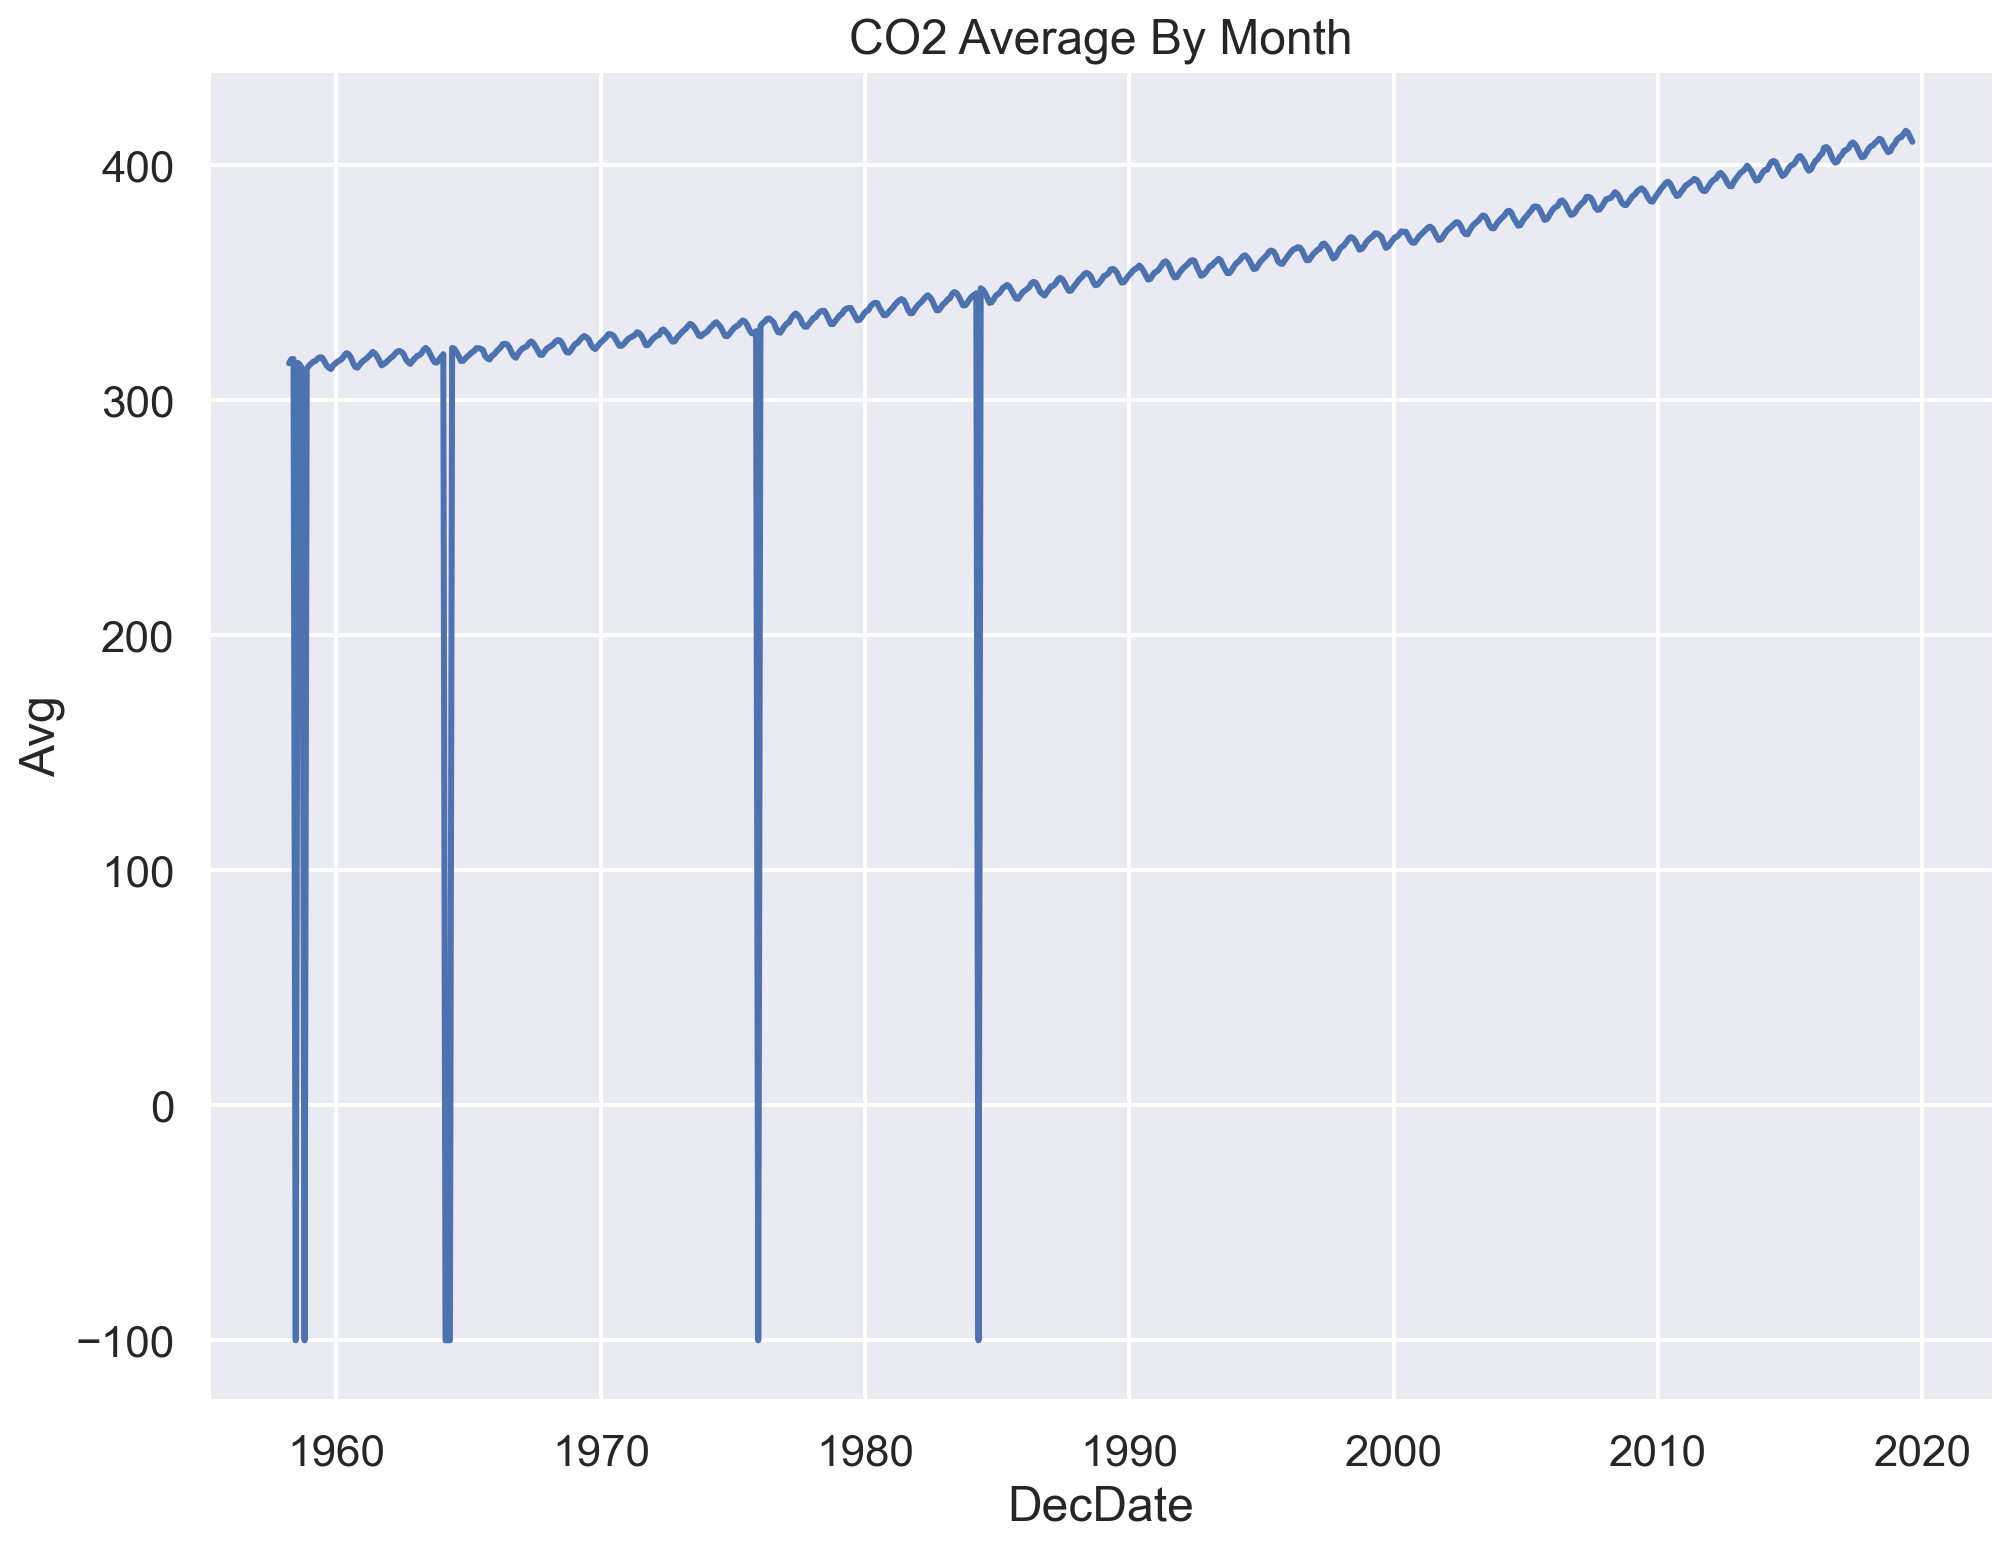
\includegraphics[keepaspectratio]{eda/eda_files/figure-pdf/cell-61-output-1.pdf}}

Since we are plotting \texttt{Avg} vs \texttt{DecDate}, we should just
focus on dealing with missing values for \texttt{Avg}.

Let's consider a few options: 1. Drop those records 2. Replace -99.99
with NaN 3. Substitute it with a likely value for the average CO2?

What do you think are the pros and cons of each possible action?

Let's examine each of these three options.

\begin{Shaded}
\begin{Highlighting}[]
\CommentTok{\# 1. Drop missing values}
\NormalTok{co2\_drop }\OperatorTok{=}\NormalTok{ co2[co2[}\StringTok{\textquotesingle{}Avg\textquotesingle{}}\NormalTok{] }\OperatorTok{\textgreater{}} \DecValTok{0}\NormalTok{]}
\NormalTok{co2\_drop.head()}
\end{Highlighting}
\end{Shaded}

\begin{longtable}[]{@{}llllllll@{}}
\toprule\noalign{}
& Yr & Mo & DecDate & Avg & Int & Trend & Days \\
\midrule\noalign{}
\endhead
\bottomrule\noalign{}
\endlastfoot
0 & 1958 & 3 & 1958.21 & 315.71 & 315.71 & 314.62 & -1 \\
1 & 1958 & 4 & 1958.29 & 317.45 & 317.45 & 315.29 & -1 \\
2 & 1958 & 5 & 1958.38 & 317.50 & 317.50 & 314.71 & -1 \\
4 & 1958 & 7 & 1958.54 & 315.86 & 315.86 & 314.98 & -1 \\
5 & 1958 & 8 & 1958.62 & 314.93 & 314.93 & 315.94 & -1 \\
\end{longtable}

\begin{Shaded}
\begin{Highlighting}[]
\CommentTok{\# 2. Replace NaN with {-}99.99}
\NormalTok{co2\_NA }\OperatorTok{=}\NormalTok{ co2.replace(}\OperatorTok{{-}}\FloatTok{99.99}\NormalTok{, np.nan)}
\NormalTok{co2\_NA.head()}
\end{Highlighting}
\end{Shaded}

\begin{longtable}[]{@{}llllllll@{}}
\toprule\noalign{}
& Yr & Mo & DecDate & Avg & Int & Trend & Days \\
\midrule\noalign{}
\endhead
\bottomrule\noalign{}
\endlastfoot
0 & 1958 & 3 & 1958.21 & 315.71 & 315.71 & 314.62 & -1 \\
1 & 1958 & 4 & 1958.29 & 317.45 & 317.45 & 315.29 & -1 \\
2 & 1958 & 5 & 1958.38 & 317.50 & 317.50 & 314.71 & -1 \\
3 & 1958 & 6 & 1958.46 & NaN & 317.10 & 314.85 & -1 \\
4 & 1958 & 7 & 1958.54 & 315.86 & 315.86 & 314.98 & -1 \\
\end{longtable}

We'll also use a third version of the data.

First, we note that the dataset already comes with a \textbf{substitute
value} for the -99.99.

From the file description:

\begin{quote}
The \texttt{interpolated} column includes average values from the
preceding column (\texttt{average}) and \textbf{interpolated values}
where data are missing. Interpolated values are computed in two
steps\ldots{}
\end{quote}

The \texttt{Int} feature has values that exactly match those in
\texttt{Avg}, except when \texttt{Avg} is -99.99, and then a
\textbf{reasonable} estimate is used instead.

So, the third version of our data will use the \texttt{Int} feature
instead of \texttt{Avg}.

\begin{Shaded}
\begin{Highlighting}[]
\CommentTok{\# 3. Use interpolated column which estimates missing Avg values}
\NormalTok{co2\_impute }\OperatorTok{=}\NormalTok{ co2.copy()}
\NormalTok{co2\_impute[}\StringTok{\textquotesingle{}Avg\textquotesingle{}}\NormalTok{] }\OperatorTok{=}\NormalTok{ co2[}\StringTok{\textquotesingle{}Int\textquotesingle{}}\NormalTok{]}
\NormalTok{co2\_impute.head()}
\end{Highlighting}
\end{Shaded}

\begin{longtable}[]{@{}llllllll@{}}
\toprule\noalign{}
& Yr & Mo & DecDate & Avg & Int & Trend & Days \\
\midrule\noalign{}
\endhead
\bottomrule\noalign{}
\endlastfoot
0 & 1958 & 3 & 1958.21 & 315.71 & 315.71 & 314.62 & -1 \\
1 & 1958 & 4 & 1958.29 & 317.45 & 317.45 & 315.29 & -1 \\
2 & 1958 & 5 & 1958.38 & 317.50 & 317.50 & 314.71 & -1 \\
3 & 1958 & 6 & 1958.46 & 317.10 & 317.10 & 314.85 & -1 \\
4 & 1958 & 7 & 1958.54 & 315.86 & 315.86 & 314.98 & -1 \\
\end{longtable}

What's a \textbf{reasonable} estimate?

To answer this question, let's zoom in on a short time period, say the
measurements in 1958 (where we know we have two missing values).

\begin{Shaded}
\begin{Highlighting}[]
\CommentTok{\# results of plotting data in 1958}

\KeywordTok{def}\NormalTok{ line\_and\_points(data, ax, title):}
    \CommentTok{\# assumes single year, hence Mo}
\NormalTok{    ax.plot(}\StringTok{\textquotesingle{}Mo\textquotesingle{}}\NormalTok{, }\StringTok{\textquotesingle{}Avg\textquotesingle{}}\NormalTok{, data}\OperatorTok{=}\NormalTok{data)}
\NormalTok{    ax.scatter(}\StringTok{\textquotesingle{}Mo\textquotesingle{}}\NormalTok{, }\StringTok{\textquotesingle{}Avg\textquotesingle{}}\NormalTok{, data}\OperatorTok{=}\NormalTok{data)}
\NormalTok{    ax.set\_xlim(}\DecValTok{2}\NormalTok{, }\DecValTok{13}\NormalTok{)}
\NormalTok{    ax.set\_title(title)}
\NormalTok{    ax.set\_xticks(np.arange(}\DecValTok{3}\NormalTok{, }\DecValTok{13}\NormalTok{))}

\KeywordTok{def}\NormalTok{ data\_year(data, year):}
    \ControlFlowTok{return}\NormalTok{ data[data[}\StringTok{"Yr"}\NormalTok{] }\OperatorTok{==} \DecValTok{1958}\NormalTok{]}
    
\CommentTok{\# uses matplotlib subplots}
\CommentTok{\# you may see more next week; focus on output for now}
\NormalTok{fig, axes }\OperatorTok{=}\NormalTok{ plt.subplots(ncols }\OperatorTok{=} \DecValTok{3}\NormalTok{, figsize}\OperatorTok{=}\NormalTok{(}\DecValTok{12}\NormalTok{, }\DecValTok{4}\NormalTok{), sharey}\OperatorTok{=}\VariableTok{True}\NormalTok{)}

\NormalTok{year }\OperatorTok{=} \DecValTok{1958}
\NormalTok{line\_and\_points(data\_year(co2\_drop, year), axes[}\DecValTok{0}\NormalTok{], title}\OperatorTok{=}\StringTok{"1. Drop Missing"}\NormalTok{)}
\NormalTok{line\_and\_points(data\_year(co2\_NA, year), axes[}\DecValTok{1}\NormalTok{], title}\OperatorTok{=}\StringTok{"2. Missing Set to NaN"}\NormalTok{)}
\NormalTok{line\_and\_points(data\_year(co2\_impute, year), axes[}\DecValTok{2}\NormalTok{], title}\OperatorTok{=}\StringTok{"3. Missing Interpolated"}\NormalTok{)}

\NormalTok{fig.suptitle(}\SpecialStringTok{f"Monthly Averages for }\SpecialCharTok{\{}\NormalTok{year}\SpecialCharTok{\}}\SpecialStringTok{"}\NormalTok{)}
\NormalTok{plt.tight\_layout()}
\end{Highlighting}
\end{Shaded}

\pandocbounded{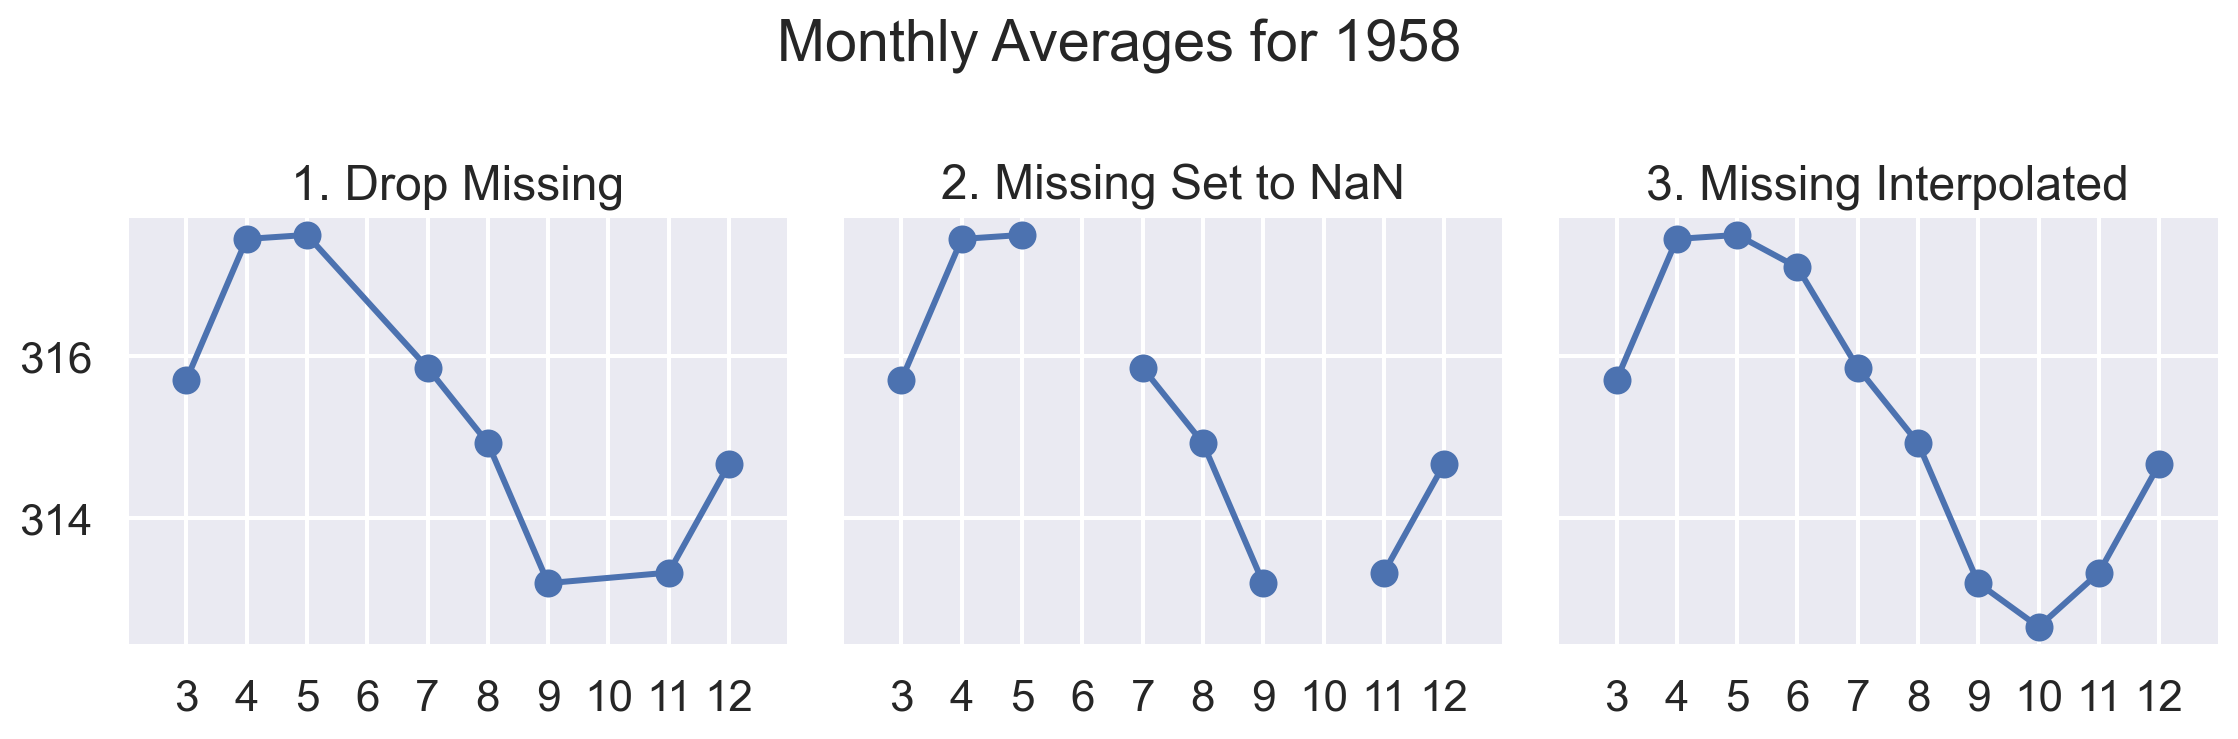
\includegraphics[keepaspectratio]{eda/eda_files/figure-pdf/cell-65-output-1.pdf}}

In the big picture since there are only 7 \texttt{Avg} values missing
(\textbf{\textless1\%} of 738 months), any of these approaches would
work.

However there is some appeal to \textbf{option C, Imputing}:

\begin{itemize}
\tightlist
\item
  Shows seasonal trends for CO2
\item
  We are plotting all months in our data as a line plot
\end{itemize}

Let's replot our original figure with option 3:

\begin{Shaded}
\begin{Highlighting}[]
\NormalTok{sns.lineplot(x}\OperatorTok{=}\StringTok{\textquotesingle{}DecDate\textquotesingle{}}\NormalTok{, y}\OperatorTok{=}\StringTok{\textquotesingle{}Avg\textquotesingle{}}\NormalTok{, data}\OperatorTok{=}\NormalTok{co2\_impute)}
\NormalTok{plt.title(}\StringTok{"CO2 Average By Month, Imputed"}\NormalTok{)}\OperatorTok{;}
\end{Highlighting}
\end{Shaded}

\pandocbounded{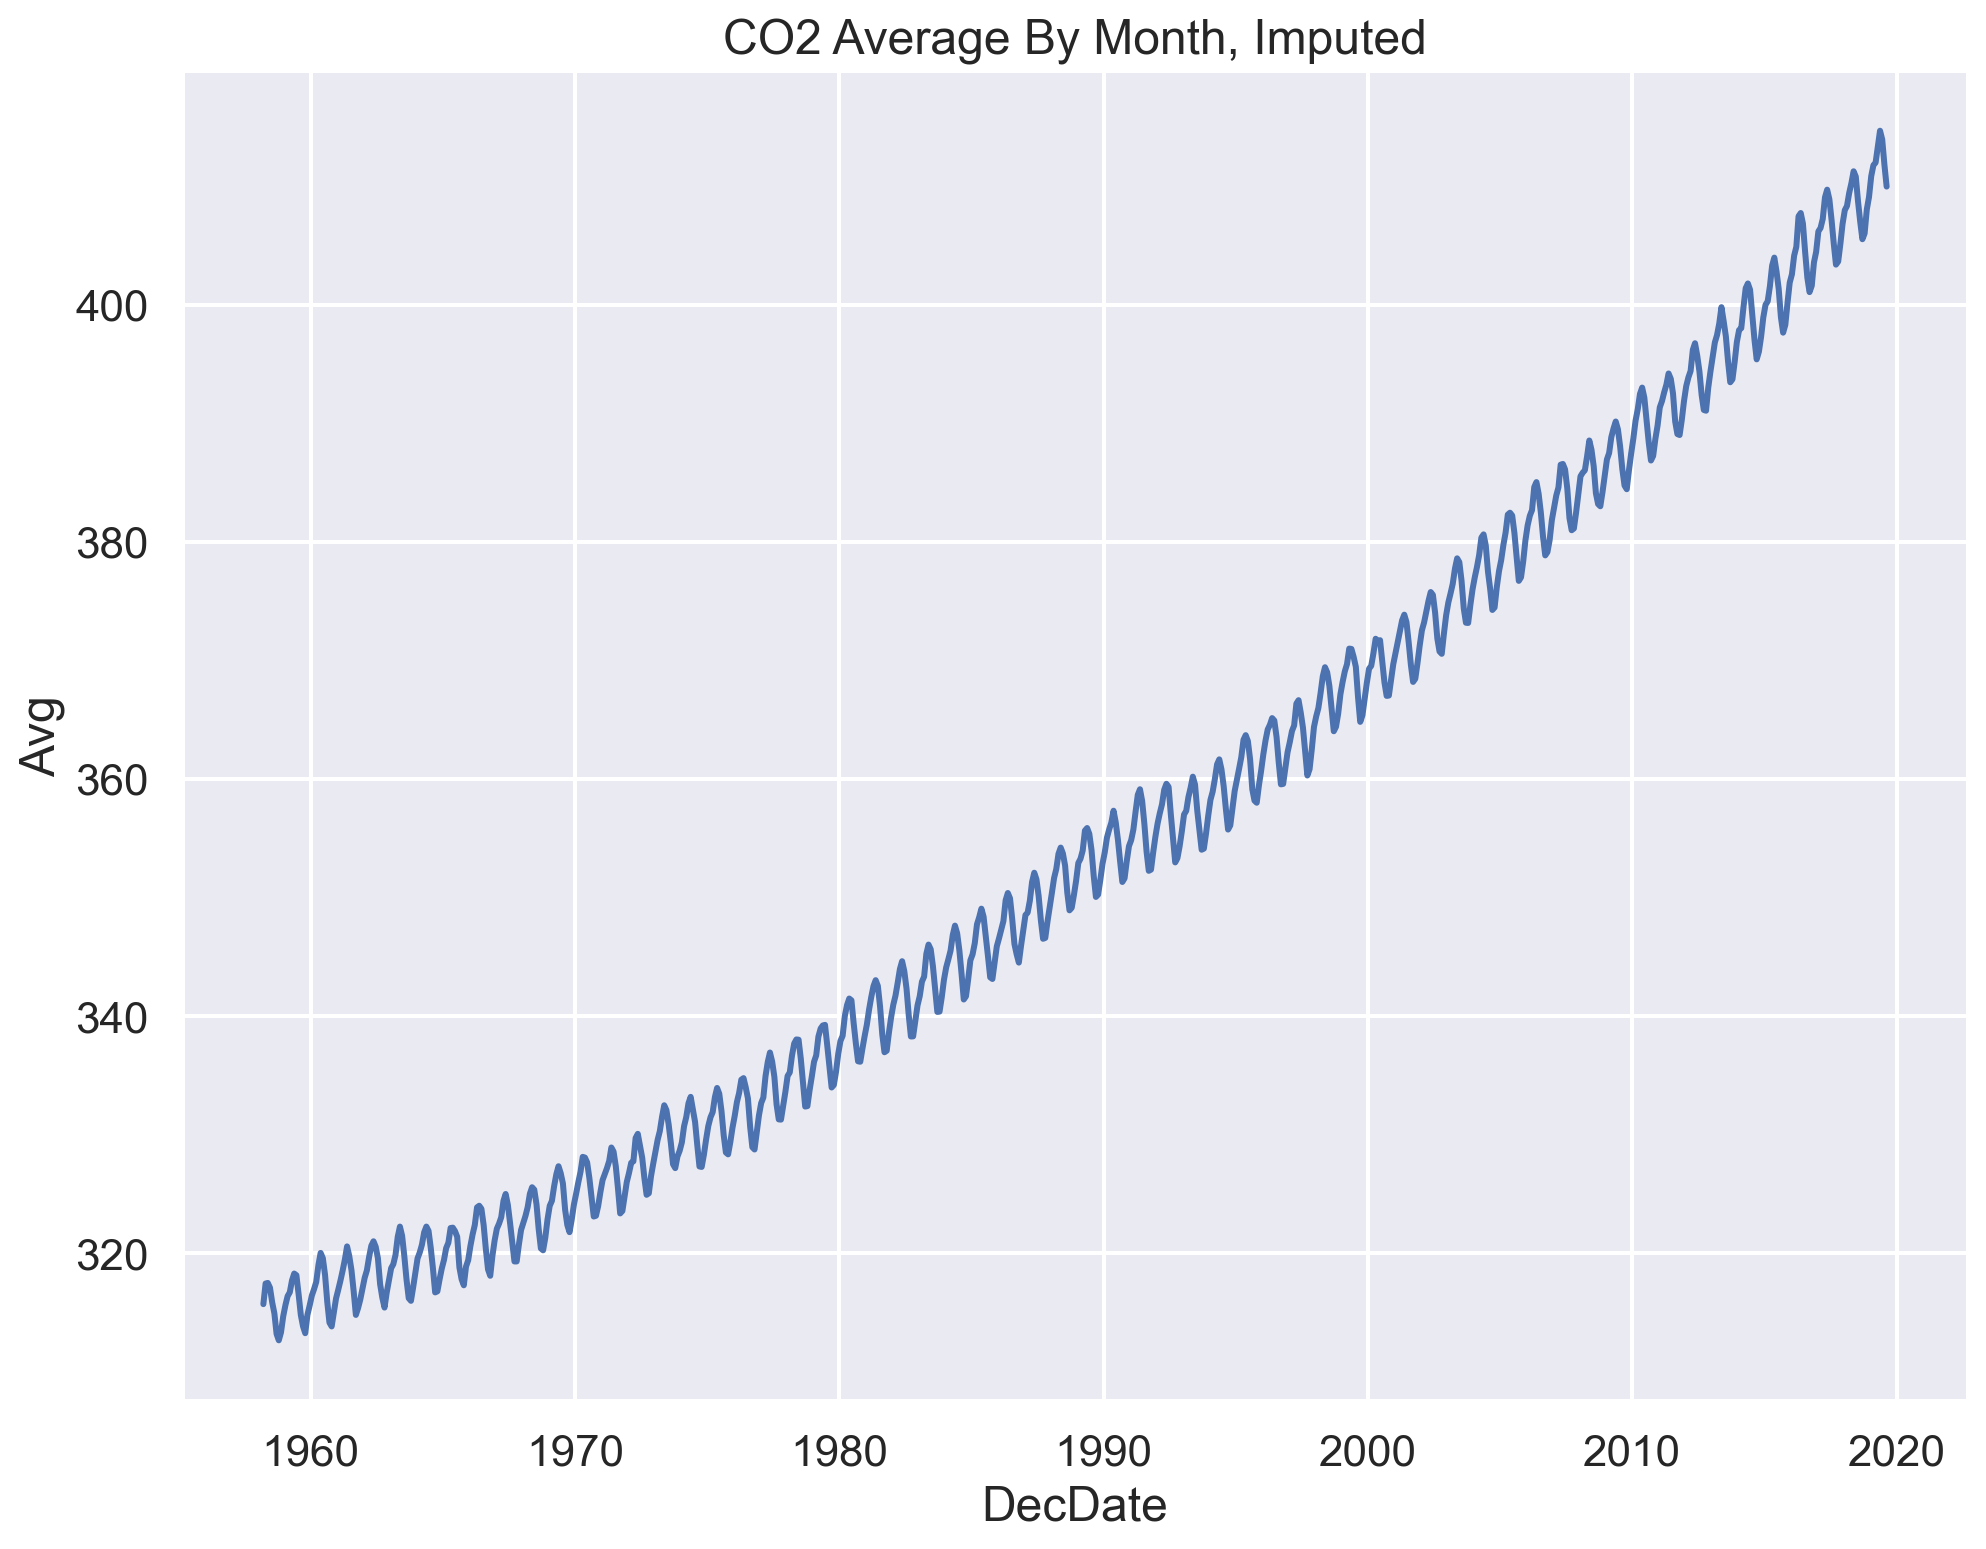
\includegraphics[keepaspectratio]{eda/eda_files/figure-pdf/cell-66-output-1.pdf}}

Looks pretty close to what we see on the NOAA
\href{https://gml.noaa.gov/ccgg/trends/}{website}!

\subsection{Presenting the Data: A Discussion on Data
Granularity}\label{presenting-the-data-a-discussion-on-data-granularity}

From the description:

\begin{itemize}
\tightlist
\item
  Monthly measurements are averages of average day measurements.
\item
  The NOAA GML website has datasets for daily/hourly measurements too.
\end{itemize}

The data you present depends on your research question.

\textbf{How do CO2 levels vary by season?}

\begin{itemize}
\tightlist
\item
  You might want to keep average monthly data.
\end{itemize}

\textbf{Are CO2 levels rising over the past 50+ years, consistent with
global warming predictions?}

\begin{itemize}
\tightlist
\item
  You might be happier with a \textbf{coarser granularity} of average
  year data!
\end{itemize}

\begin{Shaded}
\begin{Highlighting}[]
\NormalTok{co2\_year }\OperatorTok{=}\NormalTok{ co2\_impute.groupby(}\StringTok{\textquotesingle{}Yr\textquotesingle{}}\NormalTok{).mean()}
\NormalTok{sns.lineplot(x}\OperatorTok{=}\StringTok{\textquotesingle{}Yr\textquotesingle{}}\NormalTok{, y}\OperatorTok{=}\StringTok{\textquotesingle{}Avg\textquotesingle{}}\NormalTok{, data}\OperatorTok{=}\NormalTok{co2\_year)}
\NormalTok{plt.title(}\StringTok{"CO2 Average By Year"}\NormalTok{)}\OperatorTok{;}
\end{Highlighting}
\end{Shaded}

\pandocbounded{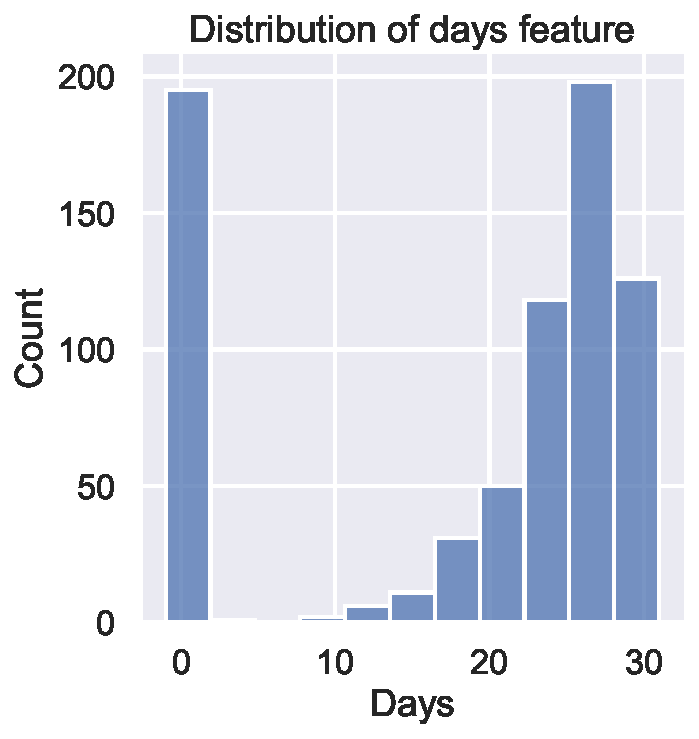
\includegraphics[keepaspectratio]{eda/eda_files/figure-pdf/cell-67-output-1.pdf}}

Indeed, we see a rise by nearly 100 ppm of CO2 since Mauna Loa began
recording in 1958.

\section{Summary}\label{summary}

We went over a lot of content this lecture; let's summarize the most
important points:

\subsection{Dealing with Missing
Values}\label{dealing-with-missing-values}

There are a few options we can take to deal with missing data:

\begin{itemize}
\tightlist
\item
  Drop missing records
\item
  Keep \texttt{NaN} missing values
\item
  Impute using an interpolated column
\end{itemize}

\subsection{EDA and Data Wrangling}\label{eda-and-data-wrangling}

There are several ways to approach EDA and Data Wrangling:

\begin{itemize}
\tightlist
\item
  Examine the \textbf{data and metadata}: what is the date, size,
  organization, and structure of the data?
\item
  Examine each \textbf{field/attribute/dimension} individually.
\item
  Examine pairs of related dimensions (e.g.~breaking down grades by
  major).
\item
  Along the way, we can:

  \begin{itemize}
  \tightlist
  \item
    \textbf{Visualize} or summarize the data.
  \item
    \textbf{Validate assumptions} about data and its collection process.
    Pay particular attention to when the data was collected.
  \item
    Identify and \textbf{address anomalies}.
  \item
    Apply data transformations and corrections (we'll cover this in the
    upcoming lecture).
  \item
    \textbf{Record everything you do!} Developing in Jupyter Notebook
    promotes \emph{reproducibility} of your own work!
  \end{itemize}
\end{itemize}

\bookmarksetup{startatroot}

\chapter{Regular Expressions}\label{regular-expressions}

\begin{tcolorbox}[enhanced jigsaw, bottomrule=.15mm, coltitle=black, breakable, opacitybacktitle=0.6, leftrule=.75mm, bottomtitle=1mm, arc=.35mm, colback=white, toptitle=1mm, left=2mm, titlerule=0mm, title=\textcolor{quarto-callout-note-color}{\faInfo}\hspace{0.5em}{Learning Outcomes}, colframe=quarto-callout-note-color-frame, rightrule=.15mm, opacityback=0, toprule=.15mm, colbacktitle=quarto-callout-note-color!10!white]

\begin{itemize}
\tightlist
\item
  Understand Python string manipulation, \texttt{pandas} \texttt{Series}
  methods
\item
  Parse and create regex, with a reference table
\item
  Use vocabulary (closure, metacharacters, groups, etc.) to describe
  regex metacharacters
\end{itemize}

\end{tcolorbox}

\section{Why Work with Text?}\label{why-work-with-text}

Last lecture, we learned of the difference between quantitative and
qualitative variable types. The latter includes string data --- the
primary focus of lecture 6. In this note, we'll discuss the necessary
tools to manipulate text: Python string manipulation and regular
expressions.

There are two main reasons for working with text.

\begin{enumerate}
\def\labelenumi{\arabic{enumi}.}
\tightlist
\item
  Canonicalization: Convert data that has multiple formats into a
  standard form.

  \begin{itemize}
  \tightlist
  \item
    By manipulating text, we can join tables with mismatched string
    labels.
  \end{itemize}
\item
  Extract information into a new feature.

  \begin{itemize}
  \tightlist
  \item
    For example, we can extract date and time features from text.
  \end{itemize}
\end{enumerate}

\section{Python String Methods}\label{python-string-methods}

First, we'll introduce a few methods useful for string manipulation. The
following table includes a number of string operations supported by
Python and \texttt{pandas}. The Python functions operate on a single
string, while their equivalent in \texttt{pandas} are
\textbf{vectorized} --- they operate on a \texttt{Series} of string
data.

\begin{longtable}[]{@{}
  >{\raggedright\arraybackslash}p{(\linewidth - 4\tabcolsep) * \real{0.3333}}
  >{\raggedright\arraybackslash}p{(\linewidth - 4\tabcolsep) * \real{0.2500}}
  >{\raggedright\arraybackslash}p{(\linewidth - 4\tabcolsep) * \real{0.3889}}@{}}
\toprule\noalign{}
\begin{minipage}[b]{\linewidth}\raggedright
Operation
\end{minipage} & \begin{minipage}[b]{\linewidth}\raggedright
Python
\end{minipage} & \begin{minipage}[b]{\linewidth}\raggedright
\texttt{Pandas} (\texttt{Series})
\end{minipage} \\
\midrule\noalign{}
\endhead
\bottomrule\noalign{}
\endlastfoot
Transformation & \begin{minipage}[t]{\linewidth}\raggedright
\begin{itemize}
\tightlist
\item
  \texttt{s.lower()}
\item
  \texttt{s.upper()}
\end{itemize}
\end{minipage} & \begin{minipage}[t]{\linewidth}\raggedright
\begin{itemize}
\tightlist
\item
  \texttt{ser.str.lower()}
\item
  \texttt{ser.str.upper()}
\end{itemize}
\end{minipage} \\
Replacement + Deletion & \begin{minipage}[t]{\linewidth}\raggedright
\begin{itemize}
\tightlist
\item
  \texttt{s.replace(\_)}
\end{itemize}
\end{minipage} & \begin{minipage}[t]{\linewidth}\raggedright
\begin{itemize}
\tightlist
\item
  \texttt{ser.str.replace(\_)}
\end{itemize}
\end{minipage} \\
Split & \begin{minipage}[t]{\linewidth}\raggedright
\begin{itemize}
\tightlist
\item
  \texttt{s.split(\_)}
\end{itemize}
\end{minipage} & \begin{minipage}[t]{\linewidth}\raggedright
\begin{itemize}
\tightlist
\item
  \texttt{ser.str.split(\_)}
\end{itemize}
\end{minipage} \\
Substring & \begin{minipage}[t]{\linewidth}\raggedright
\begin{itemize}
\tightlist
\item
  \texttt{s{[}1:4{]}}
\end{itemize}
\end{minipage} & \begin{minipage}[t]{\linewidth}\raggedright
\begin{itemize}
\tightlist
\item
  \texttt{ser.str{[}1:4{]}}
\end{itemize}
\end{minipage} \\
Membership & \begin{minipage}[t]{\linewidth}\raggedright
\begin{itemize}
\tightlist
\item
  \texttt{\textquotesingle{}\_\textquotesingle{}\ in\ s}
\end{itemize}
\end{minipage} & \begin{minipage}[t]{\linewidth}\raggedright
\begin{itemize}
\tightlist
\item
  \texttt{ser.str.contains(\_)}
\end{itemize}
\end{minipage} \\
Length & \begin{minipage}[t]{\linewidth}\raggedright
\begin{itemize}
\tightlist
\item
  \texttt{len(s)}
\end{itemize}
\end{minipage} & \begin{minipage}[t]{\linewidth}\raggedright
\begin{itemize}
\tightlist
\item
  \texttt{ser.str.len()}
\end{itemize}
\end{minipage} \\
\end{longtable}

We'll discuss the differences between Python string functions and
\texttt{pandas} \texttt{Series} methods in the following section on
canonicalization.

\subsection{Canonicalization}\label{canonicalization}

Assume we want to merge the given tables.

\begin{Shaded}
\begin{Highlighting}[]
\ImportTok{import}\NormalTok{ pandas }\ImportTok{as}\NormalTok{ pd}

\ControlFlowTok{with} \BuiltInTok{open}\NormalTok{(}\StringTok{\textquotesingle{}data/county\_and\_state.csv\textquotesingle{}}\NormalTok{) }\ImportTok{as}\NormalTok{ f:}
\NormalTok{    county\_and\_state }\OperatorTok{=}\NormalTok{ pd.read\_csv(f)}
    
\ControlFlowTok{with} \BuiltInTok{open}\NormalTok{(}\StringTok{\textquotesingle{}data/county\_and\_population.csv\textquotesingle{}}\NormalTok{) }\ImportTok{as}\NormalTok{ f:}
\NormalTok{    county\_and\_pop }\OperatorTok{=}\NormalTok{ pd.read\_csv(f)}
\end{Highlighting}
\end{Shaded}

\begin{Shaded}
\begin{Highlighting}[]
\NormalTok{display(county\_and\_state), display(county\_and\_pop)}\OperatorTok{;}
\end{Highlighting}
\end{Shaded}

\begin{longtable}[]{@{}lll@{}}
\toprule\noalign{}
& County & State \\
\midrule\noalign{}
\endhead
\bottomrule\noalign{}
\endlastfoot
0 & De Witt County & IL \\
1 & Lac qui Parle County & MN \\
2 & Lewis and Clark County & MT \\
3 & St John the Baptist Parish & LS \\
\end{longtable}

\begin{longtable}[]{@{}lll@{}}
\toprule\noalign{}
& County & Population \\
\midrule\noalign{}
\endhead
\bottomrule\noalign{}
\endlastfoot
0 & DeWitt & 16798 \\
1 & Lac Qui Parle & 8067 \\
2 & Lewis \& Clark & 55716 \\
3 & St. John the Baptist & 43044 \\
\end{longtable}

Can we convert these columns into one standard, canonical form to merge
the two tables?

\subsubsection{Canonicalization with Python String
Manipulation}\label{canonicalization-with-python-string-manipulation}

The following function uses Python string manipulation to convert a
single county name into canonical form. It does so by eliminating
whitespace, punctuation, and unnecessary text.

\begin{Shaded}
\begin{Highlighting}[]
\KeywordTok{def}\NormalTok{ canonicalize\_county(county\_name):}
    \ControlFlowTok{return}\NormalTok{ (}
\NormalTok{        county\_name}
\NormalTok{            .lower()}
\NormalTok{            .replace(}\StringTok{\textquotesingle{} \textquotesingle{}}\NormalTok{, }\StringTok{\textquotesingle{}\textquotesingle{}}\NormalTok{)}
\NormalTok{            .replace(}\StringTok{\textquotesingle{}\&\textquotesingle{}}\NormalTok{, }\StringTok{\textquotesingle{}and\textquotesingle{}}\NormalTok{)}
\NormalTok{            .replace(}\StringTok{\textquotesingle{}.\textquotesingle{}}\NormalTok{, }\StringTok{\textquotesingle{}\textquotesingle{}}\NormalTok{)}
\NormalTok{            .replace(}\StringTok{\textquotesingle{}county\textquotesingle{}}\NormalTok{, }\StringTok{\textquotesingle{}\textquotesingle{}}\NormalTok{)}
\NormalTok{            .replace(}\StringTok{\textquotesingle{}parish\textquotesingle{}}\NormalTok{, }\StringTok{\textquotesingle{}\textquotesingle{}}\NormalTok{)}
\NormalTok{    )}

\NormalTok{canonicalize\_county(}\StringTok{"St. John the Baptist"}\NormalTok{)}
\end{Highlighting}
\end{Shaded}

\begin{verbatim}
'stjohnthebaptist'
\end{verbatim}

\subsubsection{Canonicalization with Pandas Series
Methods}\label{canonicalization-with-pandas-series-methods}

Alternatively, we can use \texttt{pandas} \texttt{Series} methods to
create this standardized column. To do so, we must call the
\texttt{.str} attribute of our \texttt{Series} object prior to calling
any methods, like \texttt{.lower} and \texttt{.replace}. Notice how
these method names match their equivalent built-in Python string
functions.

Chaining multiple \texttt{Series} methods in this manner eliminates the
need to use the \texttt{map} function (as this code is vectorized).

\begin{Shaded}
\begin{Highlighting}[]
\KeywordTok{def}\NormalTok{ canonicalize\_county\_series(county\_series):}
    \ControlFlowTok{return}\NormalTok{ (}
\NormalTok{        county\_series}
\NormalTok{            .}\BuiltInTok{str}\NormalTok{.lower()}
\NormalTok{            .}\BuiltInTok{str}\NormalTok{.replace(}\StringTok{\textquotesingle{} \textquotesingle{}}\NormalTok{, }\StringTok{\textquotesingle{}\textquotesingle{}}\NormalTok{)}
\NormalTok{            .}\BuiltInTok{str}\NormalTok{.replace(}\StringTok{\textquotesingle{}\&\textquotesingle{}}\NormalTok{, }\StringTok{\textquotesingle{}and\textquotesingle{}}\NormalTok{)}
\NormalTok{            .}\BuiltInTok{str}\NormalTok{.replace(}\StringTok{\textquotesingle{}.\textquotesingle{}}\NormalTok{, }\StringTok{\textquotesingle{}\textquotesingle{}}\NormalTok{)}
\NormalTok{            .}\BuiltInTok{str}\NormalTok{.replace(}\StringTok{\textquotesingle{}county\textquotesingle{}}\NormalTok{, }\StringTok{\textquotesingle{}\textquotesingle{}}\NormalTok{)}
\NormalTok{            .}\BuiltInTok{str}\NormalTok{.replace(}\StringTok{\textquotesingle{}parish\textquotesingle{}}\NormalTok{, }\StringTok{\textquotesingle{}\textquotesingle{}}\NormalTok{)}
\NormalTok{    )}

\NormalTok{county\_and\_pop[}\StringTok{\textquotesingle{}clean\_county\_pandas\textquotesingle{}}\NormalTok{] }\OperatorTok{=}\NormalTok{ canonicalize\_county\_series(county\_and\_pop[}\StringTok{\textquotesingle{}County\textquotesingle{}}\NormalTok{])}
\NormalTok{county\_and\_state[}\StringTok{\textquotesingle{}clean\_county\_pandas\textquotesingle{}}\NormalTok{] }\OperatorTok{=}\NormalTok{ canonicalize\_county\_series(county\_and\_state[}\StringTok{\textquotesingle{}County\textquotesingle{}}\NormalTok{])}
\NormalTok{display(county\_and\_pop), display(county\_and\_state)}\OperatorTok{;}
\end{Highlighting}
\end{Shaded}

\begin{longtable}[]{@{}llll@{}}
\toprule\noalign{}
& County & Population & clean\_county\_pandas \\
\midrule\noalign{}
\endhead
\bottomrule\noalign{}
\endlastfoot
0 & DeWitt & 16798 & dewitt \\
1 & Lac Qui Parle & 8067 & lacquiparle \\
2 & Lewis \& Clark & 55716 & lewisandclark \\
3 & St. John the Baptist & 43044 & stjohnthebaptist \\
\end{longtable}

\begin{longtable}[]{@{}llll@{}}
\toprule\noalign{}
& County & State & clean\_county\_pandas \\
\midrule\noalign{}
\endhead
\bottomrule\noalign{}
\endlastfoot
0 & De Witt County & IL & dewitt \\
1 & Lac qui Parle County & MN & lacquiparle \\
2 & Lewis and Clark County & MT & lewisandclark \\
3 & St John the Baptist Parish & LS & stjohnthebaptist \\
\end{longtable}

\subsection{Extraction}\label{extraction}

Extraction explores the idea of obtaining useful information from text
data. This will be particularily important in model building, which
we'll study in a few weeks.

Say we want to read some data from a \texttt{.txt} file.

\begin{Shaded}
\begin{Highlighting}[]
\ControlFlowTok{with} \BuiltInTok{open}\NormalTok{(}\StringTok{\textquotesingle{}data/log.txt\textquotesingle{}}\NormalTok{, }\StringTok{\textquotesingle{}r\textquotesingle{}}\NormalTok{) }\ImportTok{as}\NormalTok{ f:}
\NormalTok{    log\_lines }\OperatorTok{=}\NormalTok{ f.readlines()}

\NormalTok{log\_lines}
\end{Highlighting}
\end{Shaded}

\begin{verbatim}
['169.237.46.168 - - [26/Jan/2014:10:47:58 -0800] "GET /stat141/Winter04/ HTTP/1.1" 200 2585 "http://anson.ucdavis.edu/courses/"\n',
 '193.205.203.3 - - [2/Feb/2005:17:23:6 -0800] "GET /stat141/Notes/dim.html HTTP/1.0" 404 302 "http://eeyore.ucdavis.edu/stat141/Notes/session.html"\n',
 '169.237.46.240 - "" [3/Feb/2006:10:18:37 -0800] "GET /stat141/homework/Solutions/hw1Sol.pdf HTTP/1.1"\n']
\end{verbatim}

Suppose we want to extract the day, month, year, hour, minutes, seconds,
and time zone. Unfortunately, these items are not in a fixed position
from the beginning of the string, so slicing by some fixed offset won't
work.

Instead, we can use some clever thinking. Notice how the relevant
information is contained within a set of brackets, further separated by
\texttt{/} and \texttt{:}. We can hone in on this region of text, and
split the data on these characters. Python's built-in \texttt{.split}
function makes this easy.

\begin{Shaded}
\begin{Highlighting}[]
\NormalTok{first }\OperatorTok{=}\NormalTok{ log\_lines[}\DecValTok{0}\NormalTok{] }\CommentTok{\# Only considering the first row of data}

\NormalTok{pertinent }\OperatorTok{=}\NormalTok{ first.split(}\StringTok{"["}\NormalTok{)[}\DecValTok{1}\NormalTok{].split(}\StringTok{\textquotesingle{}]\textquotesingle{}}\NormalTok{)[}\DecValTok{0}\NormalTok{]}
\NormalTok{day, month, rest }\OperatorTok{=}\NormalTok{ pertinent.split(}\StringTok{\textquotesingle{}/\textquotesingle{}}\NormalTok{)}
\NormalTok{year, hour, minute, rest }\OperatorTok{=}\NormalTok{ rest.split(}\StringTok{\textquotesingle{}:\textquotesingle{}}\NormalTok{)}
\NormalTok{seconds, time\_zone }\OperatorTok{=}\NormalTok{ rest.split(}\StringTok{\textquotesingle{} \textquotesingle{}}\NormalTok{)}
\NormalTok{day, month, year, hour, minute, seconds, time\_zone}
\end{Highlighting}
\end{Shaded}

\begin{verbatim}
('26', 'Jan', '2014', '10', '47', '58', '-0800')
\end{verbatim}

There are two problems with this code:

\begin{enumerate}
\def\labelenumi{\arabic{enumi}.}
\tightlist
\item
  Python's built-in functions limit us to extract data one record at a
  time,
\item
  The code is quite verbose.

  \begin{itemize}
  \tightlist
  \item
    This is a larger issue that is trickier to solve
  \end{itemize}
\end{enumerate}

In the next section, we'll introduce regular expressions - a tool that
solves problem 2.

\section{RegEx Basics}\label{regex-basics}

A \textbf{regular expression (``RegEx'')} is a sequence of characters
that specifies a search pattern. They are written to extract specific
information from text. Regular expressions are essentially part of a
smaller programming language embedded in Python, made available through
the \texttt{re} module. As such, they have a stand-alone syntax and
methods for various capabilities.

Regular expressions are useful in many applications beyond data science.
For example, Social Security Numbers (SSNs) are often validated with
regular expressions.

\begin{Shaded}
\begin{Highlighting}[]
\CommentTok{r"[0{-}9]\{3\}{-}[0{-}9]\{2\}{-}[0{-}9]\{4\}"} \CommentTok{\# Regular Expression Syntax}

\CommentTok{\# 3 of any digit, then a dash,}
\CommentTok{\# then 2 of any digit, then a dash,}
\CommentTok{\# then 4 of any digit}
\end{Highlighting}
\end{Shaded}

\begin{verbatim}
'[0-9]{3}-[0-9]{2}-[0-9]{4}'
\end{verbatim}

There are a ton of resources to learn and experiment with regular
expressions. A few are provided below:

\begin{itemize}
\tightlist
\item
  \href{https://docs.python.org/3/howto/regex.html}{Official Regex
  Guide}
\item
  \href{https://ds100.org/sp22/resources/assets/hw/regex_reference.pdf}{Data
  100 Reference Sheet}
\item
  \href{https://regex101.com/}{Regex101.com}

  \begin{itemize}
  \tightlist
  \item
    Be sure to check Python under the category on the left.
  \end{itemize}
\end{itemize}

\subsection{Basics RegEx Syntax}\label{basics-regex-syntax}

There are four basic operations with regular expressions.

\begin{longtable}[]{@{}
  >{\raggedright\arraybackslash}p{(\linewidth - 8\tabcolsep) * \real{0.2500}}
  >{\raggedright\arraybackslash}p{(\linewidth - 8\tabcolsep) * \real{0.1875}}
  >{\raggedright\arraybackslash}p{(\linewidth - 8\tabcolsep) * \real{0.1771}}
  >{\raggedright\arraybackslash}p{(\linewidth - 8\tabcolsep) * \real{0.1458}}
  >{\raggedright\arraybackslash}p{(\linewidth - 8\tabcolsep) * \real{0.2083}}@{}}
\toprule\noalign{}
\begin{minipage}[b]{\linewidth}\raggedright
Operation
\end{minipage} & \begin{minipage}[b]{\linewidth}\raggedright
Order
\end{minipage} & \begin{minipage}[b]{\linewidth}\raggedright
Syntax Example
\end{minipage} & \begin{minipage}[b]{\linewidth}\raggedright
Matches
\end{minipage} & \begin{minipage}[b]{\linewidth}\raggedright
Doesn't Match
\end{minipage} \\
\midrule\noalign{}
\endhead
\bottomrule\noalign{}
\endlastfoot
\texttt{Or}: \texttt{\textbar{}} & 4 & AA\textbar BAAB & AA BAAB & every
other string \\
\texttt{Concatenation} & 3 & AABAAB & AABAAB & every other string \\
\texttt{Closure}: \texttt{*} (zero or more) & 2 & AB*A & AA ABBBBBBA &
AB ABABA \\
\texttt{Group}: \texttt{()} (parenthesis) & 1 & A(A\textbar B)AAB (AB)*A
& AAAAB ABAAB A ABABABABA & every other string AA ABBA \\
\end{longtable}

Notice how these metacharacter operations are ordered. Rather than being
literal characters, these \textbf{metacharacters} manipulate adjacent
characters. \texttt{()} takes precedence, followed by \texttt{*}, and
finally \texttt{\textbar{}}. This allows us to differentiate between
very different regex commands like \texttt{AB*} and \texttt{(AB)*}. The
former reads ``\texttt{A} then zero or more copies of \texttt{B}'',
while the latter specifies ``zero or more copies of \texttt{AB}''.

\subsubsection{Examples}\label{examples}

\textbf{Question 1}: Give a regular expression that matches
\texttt{moon}, \texttt{moooon}, etc. Your expression should match any
even number of \texttt{o}s except zero (i.e.~don't match \texttt{mn}).

Answer1

\texttt{moo(oo)*n}

\begin{itemize}
\tightlist
\item
  Hardcoding \texttt{oo} before the capture group ensures that
  \texttt{mn} is not matched.
\item
  A capture group of \texttt{(oo)*} ensures the number of \texttt{o}'s
  is even.
\end{itemize}

\textbf{Question 2}: Using only basic operations, formulate a regex that
matches \texttt{muun}, \texttt{muuuun}, \texttt{moon}, \texttt{moooon},
etc. Your expression should match any even number of \texttt{u}s or
\texttt{o}s except zero (i.e.~don't match \texttt{mn}).

Answer2

\texttt{m(uu(uu)*\textbar{}oo(oo)*)n}

\begin{itemize}
\tightlist
\item
  The leading \texttt{m} and trailing \texttt{n} ensures that only
  strings beginning with \texttt{m} and ending with \texttt{n} are
  matched.
\item
  Notice how the outer capture group surrounds the \texttt{\textbar{}}.

  \begin{itemize}
  \tightlist
  \item
    Consider the regex \texttt{m(uu(uu)*)\textbar{}(oo(oo)*)n}. This
    incorrectly matches \texttt{muu} and \texttt{oooon}.

    \begin{itemize}
    \tightlist
    \item
      Each OR clause is everything to the left and right of
      \texttt{\textbar{}}. The incorrect solution matches only half of
      the string, and ignores either the beginning \texttt{m} or
      trailing \texttt{n}.
    \item
      A set of parenthesis must surround \texttt{\textbar{}}. That way,
      each OR clause is everything to the left and right of
      \texttt{\textbar{}} \textbf{within} the group. This ensures both
      the beginning \texttt{m} \emph{and} trailing \texttt{n} are
      matched.
    \end{itemize}
  \end{itemize}
\end{itemize}

\section{RegEx Expanded}\label{regex-expanded}

Provided below are more complex regular expression functions.

\begin{longtable}[]{@{}
  >{\raggedright\arraybackslash}p{(\linewidth - 6\tabcolsep) * \real{0.4667}}
  >{\raggedright\arraybackslash}p{(\linewidth - 6\tabcolsep) * \real{0.1714}}
  >{\raggedright\arraybackslash}p{(\linewidth - 6\tabcolsep) * \real{0.1619}}
  >{\raggedright\arraybackslash}p{(\linewidth - 6\tabcolsep) * \real{0.1810}}@{}}
\toprule\noalign{}
\begin{minipage}[b]{\linewidth}\raggedright
Operation
\end{minipage} & \begin{minipage}[b]{\linewidth}\raggedright
Syntax Example
\end{minipage} & \begin{minipage}[b]{\linewidth}\raggedright
Matches
\end{minipage} & \begin{minipage}[b]{\linewidth}\raggedright
Doesn't Match
\end{minipage} \\
\midrule\noalign{}
\endhead
\bottomrule\noalign{}
\endlastfoot
\texttt{Any\ Character}: \texttt{.} (except newline) & .U.U.U. & CUMULUS
JUGULUM & SUCCUBUS TUMULTUOUS \\
\texttt{Character\ Class}: \texttt{{[}{]}} (match one character in
\texttt{{[}{]}}) & {[}A-Za-z{]}{[}a-z{]}* & word Capitalized & camelCase
4illegal \\
\texttt{Repeated\ "a"\ Times}: \texttt{\{a\}} & j{[}aeiou{]}\{3\}hn &
jaoehn jooohn & jhn jaeiouhn \\
\texttt{Repeated\ "from\ a\ to\ b"\ Times}: \texttt{\{a,\ b\}} &
j{[}ou{]}\{1,2\}hn & john juohn & jhn jooohn \\
\texttt{At\ Least\ One}: \texttt{+} & jo+hn & john joooooohn & jhn
jjohn \\
\texttt{Zero\ or\ One}: \texttt{?} & joh?n & jon john & any other
string \\
\end{longtable}

A character class matches a single character in its class. These
characters can be hardcoded ------ in the case of \texttt{{[}aeiou{]}}
------ or shorthand can be specified to mean a range of characters.
Examples include:

\begin{enumerate}
\def\labelenumi{\arabic{enumi}.}
\tightlist
\item
  \texttt{{[}A-Z{]}}: Any capitalized letter
\item
  \texttt{{[}a-z{]}}: Any lowercase letter
\item
  \texttt{{[}0-9{]}}: Any single digit
\item
  \texttt{{[}A-Za-z{]}}: Any capitalized or lowercase letter
\item
  \texttt{{[}A-Za-z0-9{]}}: Any capitalized or lowercase letter or
  single digit
\end{enumerate}

\subsubsection{Examples}\label{examples-1}

Let's analyze a few examples of complex regular expressions.

\begin{longtable}[]{@{}
  >{\raggedright\arraybackslash}p{(\linewidth - 2\tabcolsep) * \real{0.4722}}
  >{\raggedright\arraybackslash}p{(\linewidth - 2\tabcolsep) * \real{0.4722}}@{}}
\toprule\noalign{}
\begin{minipage}[b]{\linewidth}\raggedright
Matches
\end{minipage} & \begin{minipage}[b]{\linewidth}\raggedright
Does Not Match
\end{minipage} \\
\midrule\noalign{}
\endhead
\bottomrule\noalign{}
\endlastfoot
\begin{minipage}[t]{\linewidth}\raggedright
\begin{enumerate}
\def\labelenumi{\arabic{enumi}.}
\tightlist
\item
  \texttt{.*SPB.*}
\end{enumerate}
\end{minipage} & \\
RASPBERRY SPBOO & SUBSPACE SUBSPECIES \\
\begin{minipage}[t]{\linewidth}\raggedright
\begin{enumerate}
\def\labelenumi{\arabic{enumi}.}
\setcounter{enumi}{1}
\tightlist
\item
  \texttt{{[}0-9{]}\{3\}-{[}0-9{]}\{2\}-{[}0-9{]}\{4\}}
\end{enumerate}
\end{minipage} & \\
231-41-5121 573-57-1821 & 231415121 57-3571821 \\
\begin{minipage}[t]{\linewidth}\raggedright
\begin{enumerate}
\def\labelenumi{\arabic{enumi}.}
\setcounter{enumi}{2}
\tightlist
\item
  \texttt{{[}a-z{]}+@({[}a-z{]}+\textbackslash{}.)+(edu\textbar{}com)}
\end{enumerate}
\end{minipage} & \\
horse@pizza.com horse@pizza.food.com & frank\_99@yahoo.com hug@cs \\
\end{longtable}

\textbf{Explanations}

\begin{enumerate}
\def\labelenumi{\arabic{enumi}.}
\tightlist
\item
  \texttt{.*SPB.*} only matches strings that contain the substring
  \texttt{SPB}.

  \begin{itemize}
  \tightlist
  \item
    The \texttt{.*} metacharacter matches any amount of non-negative
    characters. Newlines do not count.\\
  \end{itemize}
\item
  This regular expression matches 3 of any digit, then a dash, then 2 of
  any digit, then a dash, then 4 of any digit.

  \begin{itemize}
  \tightlist
  \item
    You'll recognize this as the familiar Social Security Number regular
    expression.
  \end{itemize}
\item
  Matches any email with a \texttt{com} or \texttt{edu} domain, where
  all characters of the email are letters.

  \begin{itemize}
  \tightlist
  \item
    At least one \texttt{.} must precede the domain name. Including a
    backslash \texttt{\textbackslash{}} before any metacharacter (in
    this case, the \texttt{.}) tells RegEx to match that character
    exactly.
  \end{itemize}
\end{enumerate}

\section{Convenient RegEx}\label{convenient-regex}

Here are a few more convenient regular expressions.

\begin{longtable}[]{@{}
  >{\raggedright\arraybackslash}p{(\linewidth - 6\tabcolsep) * \real{0.4667}}
  >{\raggedright\arraybackslash}p{(\linewidth - 6\tabcolsep) * \real{0.1714}}
  >{\raggedright\arraybackslash}p{(\linewidth - 6\tabcolsep) * \real{0.1619}}
  >{\raggedright\arraybackslash}p{(\linewidth - 6\tabcolsep) * \real{0.1810}}@{}}
\toprule\noalign{}
\begin{minipage}[b]{\linewidth}\raggedright
Operation
\end{minipage} & \begin{minipage}[b]{\linewidth}\raggedright
Syntax Example
\end{minipage} & \begin{minipage}[b]{\linewidth}\raggedright
Matches
\end{minipage} & \begin{minipage}[b]{\linewidth}\raggedright
Doesn't Match
\end{minipage} \\
\midrule\noalign{}
\endhead
\bottomrule\noalign{}
\endlastfoot
\texttt{built\ in\ character\ class} & \texttt{\textbackslash{}w+}
\texttt{\textbackslash{}d+} \texttt{\textbackslash{}s+} & Fawef\_03
231123 \texttt{whitespace} & this person 423 people
\texttt{non-whitespace} \\
\texttt{character\ class\ negation}: \texttt{{[}\^{}{]}} (everything
except the given characters) & {[}\^{}a-z{]}+. & PEPPERS3982 17211!↑å &
porch CLAmS \\
\texttt{escape\ character}: \texttt{\textbackslash{}} (match the literal
next character) & cow\textbackslash.com & cow.com & cowscom \\
\texttt{beginning\ of\ line}: \texttt{\^{}} & \^{}ark & ark two ark o
ark & dark \\
\texttt{end\ of\ line}: \texttt{\$} & ark\$ & dark ark o ark & ark
two \\
\texttt{lazy\ version\ of\ zero\ or\ more} : \texttt{*?} & 5.*?5 & 5005
55 & 5005005 \\
\end{longtable}

\subsection{Greediness}\label{greediness}

In order to fully understand the last operation in the table, we have to
discuss greediness. RegEx is greedy -- it will look for the longest
possible match in a string. To motivate this with an example, consider
the pattern
\texttt{\textless{}div\textgreater{}.*\textless{}/div\textgreater{}}. In
the sentence below, we would hope that the bolded portions would be
matched:

``This is a
\textbf{\textless div\textgreater example\textless/div\textgreater{}} of
greediness
\textbf{\textless div\textgreater in\textless/div\textgreater{}} regular
expressions.''

However, in reality, RegEx captures far more of the sentence. The way
RegEx processes the text given that pattern is as follows:

\begin{enumerate}
\def\labelenumi{\arabic{enumi}.}
\item
  ``Look for the exact string \textless{}\div\textgreater{}''
\item
  Then, ``look for any character 0 or more times''
\item
  Then, ``look for the exact string \textless/div\textgreater{}''
\end{enumerate}

The result would be all the characters starting from the leftmost
\textless div\textgreater{} and the rightmost
\textless/div\textgreater{} (inclusive):

``This is a
\textbf{\textless div\textgreater example\textless/div\textgreater{} of
greediness \textless div\textgreater in\textless/div\textgreater{}}
regular expressions.''

We can fix this by making our pattern non-greedy,
\texttt{\textless{}div\textgreater{}.*?\textless{}/div\textgreater{}}.
You can read up more in the documentation
\href{https://docs.python.org/3/howto/regex.html\#greedy-versus-non-greedy}{here}.

\subsection{Examples}\label{examples-2}

Let's revisit our earlier problem of extracting date/time data from the
given \texttt{.txt} files. Here is how the data looked.

\begin{Shaded}
\begin{Highlighting}[]
\NormalTok{log\_lines[}\DecValTok{0}\NormalTok{]}
\end{Highlighting}
\end{Shaded}

\begin{verbatim}
'169.237.46.168 - - [26/Jan/2014:10:47:58 -0800] "GET /stat141/Winter04/ HTTP/1.1" 200 2585 "http://anson.ucdavis.edu/courses/"\n'
\end{verbatim}

\textbf{Question}: Give a regular expression that matches everything
contained within and including the brackets - the day, month, year,
hour, minutes, seconds, and time zone.

Answer

\texttt{\textbackslash{}{[}.*\textbackslash{}{]}}

\begin{itemize}
\tightlist
\item
  Notice how matching the literal \texttt{{[}} and \texttt{{]}} is
  necessary. Therefore, an escape character \texttt{\textbackslash{}} is
  required before both \texttt{{[}} and \texttt{{]}} --- otherwise these
  metacharacters will match character classes.
\item
  We need to match a particular format between \texttt{{[}} and
  \texttt{{]}}. For this example, \texttt{.*} will suffice.
\end{itemize}

\textbf{Alternative Solution}:
\texttt{\textbackslash{}{[}\textbackslash{}w+/\textbackslash{}w+/\textbackslash{}w+:\textbackslash{}w+:\textbackslash{}w+:\textbackslash{}w+\textbackslash{}s-\textbackslash{}w+\textbackslash{}{]}}

\begin{itemize}
\tightlist
\item
  This solution is much safer.

  \begin{itemize}
  \tightlist
  \item
    Imagine the data between \texttt{{[}} and \texttt{{]}} was garbage -
    \texttt{.*} will still match that.
  \item
    The alternate solution will only match data that follows the correct
    format.
  \end{itemize}
\end{itemize}

\section{Regex in Python and Pandas (RegEx
Groups)}\label{regex-in-python-and-pandas-regex-groups}

\subsection{Canonicalization}\label{canonicalization-1}

\subsubsection{Canonicalization with
RegEx}\label{canonicalization-with-regex}

Earlier in this note, we examined the process of canonicalization using
\texttt{python} string manipulation and \texttt{pandas} \texttt{Series}
methods. However, we mentioned this approach had a major flaw: our code
was unnecessarily verbose. Equipped with our knowledge of regular
expressions, let's fix this.

To do so, we need to understand a few functions in the \texttt{re}
module. The first of these is the substitute function:
\texttt{re.sub(pattern,\ rep1,\ text)}. It behaves similarly to
\texttt{python}'s built-in \texttt{.replace} function, and returns text
with all instances of \texttt{pattern} replaced by \texttt{rep1}.

The regular expression here removes text surrounded by
\texttt{\textless{}\textgreater{}} (also known as HTML tags).

In order, the pattern matches \ldots{} 1. a single \texttt{\textless{}}
2. any character that is not a \texttt{\textgreater{}} : div, td
valign\ldots, /td, /div 3. a single \texttt{\textgreater{}}

Any substring in \texttt{text} that fulfills all three conditions will
be replaced by \texttt{\textquotesingle{}\textquotesingle{}}.

\begin{Shaded}
\begin{Highlighting}[]
\ImportTok{import}\NormalTok{ re}

\NormalTok{text }\OperatorTok{=} \StringTok{"\textless{}div\textgreater{}\textless{}td valign=\textquotesingle{}top\textquotesingle{}\textgreater{}Moo\textless{}/td\textgreater{}\textless{}/div\textgreater{}"}
\NormalTok{pattern }\OperatorTok{=} \VerbatimStringTok{r"\textless{}[\^{}\textgreater{}]+\textgreater{}"}
\NormalTok{re.sub(pattern, }\StringTok{\textquotesingle{}\textquotesingle{}}\NormalTok{, text) }
\end{Highlighting}
\end{Shaded}

\begin{verbatim}
'Moo'
\end{verbatim}

Notice the \texttt{r} preceding the regular expression pattern; this
specifies the regular expression is a raw string. Raw strings do not
recognize escape sequences (i.e., the Python newline metacharacter
\texttt{\textbackslash{}n}). This makes them useful for regular
expressions, which often contain literal \texttt{\textbackslash{}}
characters.

In other words, don't forget to tag your RegEx with an \texttt{r}.

\subsubsection{\texorpdfstring{Canonicalization with
\texttt{pandas}}{Canonicalization with pandas}}\label{canonicalization-with-pandas}

We can also use regular expressions with \texttt{pandas} \texttt{Series}
methods. This gives us the benefit of operating on an entire column of
data as opposed to a single value. The code is simple:
\texttt{ser.str.replace(pattern,\ repl,\ regex=True}).

Consider the following \texttt{DataFrame} \texttt{html\_data} with a
single column.

\begin{Shaded}
\begin{Highlighting}[]
\NormalTok{data }\OperatorTok{=}\NormalTok{ \{}\StringTok{"HTML"}\NormalTok{: [}\StringTok{"\textless{}div\textgreater{}\textless{}td valign=\textquotesingle{}top\textquotesingle{}\textgreater{}Moo\textless{}/td\textgreater{}\textless{}/div\textgreater{}"}\NormalTok{, }\OperatorTok{\textbackslash{}}
                 \StringTok{"\textless{}a href=\textquotesingle{}http://ds100.org\textquotesingle{}\textgreater{}Link\textless{}/a\textgreater{}"}\NormalTok{, }\OperatorTok{\textbackslash{}}
                 \StringTok{"\textless{}b\textgreater{}Bold text\textless{}/b\textgreater{}"}\NormalTok{]\}}
\NormalTok{html\_data }\OperatorTok{=}\NormalTok{ pd.DataFrame(data)}
\end{Highlighting}
\end{Shaded}

\begin{Shaded}
\begin{Highlighting}[]
\NormalTok{html\_data}
\end{Highlighting}
\end{Shaded}

\begin{longtable}[]{@{}ll@{}}
\toprule\noalign{}
& HTML \\
\midrule\noalign{}
\endhead
\bottomrule\noalign{}
\endlastfoot
0 & \textless div\textgreater\textless td
valign=\textquotesingle top\textquotesingle\textgreater Moo\textless/td\textgreater\textless/div\textgreater{} \\
1 & \textless a
href=\textquotesingle http://ds100.org\textquotesingle\textgreater Link\textless/a\textgreater{} \\
2 & \textless b\textgreater Bold text\textless/b\textgreater{} \\
\end{longtable}

\begin{Shaded}
\begin{Highlighting}[]
\NormalTok{pattern }\OperatorTok{=} \VerbatimStringTok{r"\textless{}[\^{}\textgreater{}]+\textgreater{}"}
\NormalTok{html\_data[}\StringTok{\textquotesingle{}HTML\textquotesingle{}}\NormalTok{].}\BuiltInTok{str}\NormalTok{.replace(pattern, }\StringTok{\textquotesingle{}\textquotesingle{}}\NormalTok{, regex}\OperatorTok{=}\VariableTok{True}\NormalTok{)}
\end{Highlighting}
\end{Shaded}

\begin{verbatim}
0          Moo
1         Link
2    Bold text
Name: HTML, dtype: object
\end{verbatim}

\subsection{Extraction}\label{extraction-1}

\subsubsection{Extraction with RegEx}\label{extraction-with-regex}

Just like with canonicalization, the \texttt{re} module provides
capability to extract relevant text from a string:
\texttt{re.findall(pattern,\ text)}. This function returns a list of all
matches to \texttt{pattern}.

Using the familiar regular expression for Social Security Numbers:

\begin{Shaded}
\begin{Highlighting}[]
\NormalTok{text }\OperatorTok{=} \StringTok{"My social security number is 123{-}45{-}6789 bro, or maybe it’s 321{-}45{-}6789."}
\NormalTok{pattern }\OperatorTok{=} \VerbatimStringTok{r"[0{-}9]}\SpecialCharTok{\{3\}}\VerbatimStringTok{{-}[0{-}9]}\SpecialCharTok{\{2\}}\VerbatimStringTok{{-}[0{-}9]}\SpecialCharTok{\{4\}}\VerbatimStringTok{"}
\NormalTok{re.findall(pattern, text)  }
\end{Highlighting}
\end{Shaded}

\begin{verbatim}
['123-45-6789', '321-45-6789']
\end{verbatim}

\subsubsection{\texorpdfstring{Extraction with
\texttt{pandas}}{Extraction with pandas}}\label{extraction-with-pandas}

\texttt{pandas} similarily provides extraction functionality on a
\texttt{Series} of data: \texttt{ser.str.findall(pattern)}

Consider the following \texttt{DataFrame} \texttt{ssn\_data}.

\begin{Shaded}
\begin{Highlighting}[]
\NormalTok{data }\OperatorTok{=}\NormalTok{ \{}\StringTok{"SSN"}\NormalTok{: [}\StringTok{"987{-}65{-}4321"}\NormalTok{, }\StringTok{"forty"}\NormalTok{, }\OperatorTok{\textbackslash{}}
                \StringTok{"123{-}45{-}6789 bro or 321{-}45{-}6789"}\NormalTok{,}
               \StringTok{"999{-}99{-}9999"}\NormalTok{]\}}
\NormalTok{ssn\_data }\OperatorTok{=}\NormalTok{ pd.DataFrame(data)}
\end{Highlighting}
\end{Shaded}

\begin{Shaded}
\begin{Highlighting}[]
\NormalTok{ssn\_data}
\end{Highlighting}
\end{Shaded}

\begin{longtable}[]{@{}ll@{}}
\toprule\noalign{}
& SSN \\
\midrule\noalign{}
\endhead
\bottomrule\noalign{}
\endlastfoot
0 & 987-65-4321 \\
1 & forty \\
2 & 123-45-6789 bro or 321-45-6789 \\
3 & 999-99-9999 \\
\end{longtable}

\begin{Shaded}
\begin{Highlighting}[]
\NormalTok{ssn\_data[}\StringTok{"SSN"}\NormalTok{].}\BuiltInTok{str}\NormalTok{.findall(pattern)}
\end{Highlighting}
\end{Shaded}

\begin{verbatim}
0                 [987-65-4321]
1                            []
2    [123-45-6789, 321-45-6789]
3                 [999-99-9999]
Name: SSN, dtype: object
\end{verbatim}

This function returns a list for every row containing the pattern
matches in a given string.

As you may expect, there are similar \texttt{pandas} equivalents for
other \texttt{re} functions as well. \texttt{Series.str.extract} takes
in a pattern and returns a \texttt{DataFrame} of each capture group's
first match in the string. In contrast, \texttt{Series.str.extractall}
returns a multi-indexed \texttt{DataFrame} of all matches for each
capture group. You can see the difference in the outputs below:

\begin{Shaded}
\begin{Highlighting}[]
\NormalTok{pattern\_cg }\OperatorTok{=} \VerbatimStringTok{r"([0{-}9]}\SpecialCharTok{\{3\}}\VerbatimStringTok{){-}([0{-}9]}\SpecialCharTok{\{2\}}\VerbatimStringTok{){-}([0{-}9]}\SpecialCharTok{\{4\}}\VerbatimStringTok{)"}
\NormalTok{ssn\_data[}\StringTok{"SSN"}\NormalTok{].}\BuiltInTok{str}\NormalTok{.extract(pattern\_cg)}
\end{Highlighting}
\end{Shaded}

\begin{longtable}[]{@{}llll@{}}
\toprule\noalign{}
& 0 & 1 & 2 \\
\midrule\noalign{}
\endhead
\bottomrule\noalign{}
\endlastfoot
0 & 987 & 65 & 4321 \\
1 & NaN & NaN & NaN \\
2 & 123 & 45 & 6789 \\
3 & 999 & 99 & 9999 \\
\end{longtable}

\begin{Shaded}
\begin{Highlighting}[]
\NormalTok{ssn\_data[}\StringTok{"SSN"}\NormalTok{].}\BuiltInTok{str}\NormalTok{.extractall(pattern\_cg)}
\end{Highlighting}
\end{Shaded}

\begin{longtable}[]{@{}lllll@{}}
\toprule\noalign{}
& & 0 & 1 & 2 \\
& match & & & \\
\midrule\noalign{}
\endhead
\bottomrule\noalign{}
\endlastfoot
0 & 0 & 987 & 65 & 4321 \\
\multirow{2}{=}{2} & 0 & 123 & 45 & 6789 \\
& 1 & 321 & 45 & 6789 \\
3 & 0 & 999 & 99 & 9999 \\
\end{longtable}

\subsection{Regular Expression Capture
Groups}\label{regular-expression-capture-groups}

Earlier we used parentheses \texttt{(} \texttt{)} to specify the highest
order of operation in regular expressions. However, they have another
meaning; parentheses are often used to represent \textbf{capture
groups}. Capture groups are essentially, a set of smaller regular
expressions that match multiple substrings in text data.

Let's take a look at an example.

\subsubsection{Example 1}\label{example-1}

\begin{Shaded}
\begin{Highlighting}[]
\NormalTok{text }\OperatorTok{=} \StringTok{"Observations: 03:04:53 {-} Horse awakens. }\CharTok{\textbackslash{}}
\StringTok{        03:05:14 {-} Horse goes back to sleep."}
\end{Highlighting}
\end{Shaded}

Say we want to capture all occurences of time data (hour, minute, and
second) as \emph{separate entities}.

\begin{Shaded}
\begin{Highlighting}[]
\NormalTok{pattern\_1 }\OperatorTok{=} \VerbatimStringTok{r"(\textbackslash{}d\textbackslash{}d):(\textbackslash{}d\textbackslash{}d):(\textbackslash{}d\textbackslash{}d)"}
\NormalTok{re.findall(pattern\_1, text)}
\end{Highlighting}
\end{Shaded}

\begin{verbatim}
[('03', '04', '53'), ('03', '05', '14')]
\end{verbatim}

Notice how the given pattern has 3 capture groups, each specified by the
regular expression \texttt{(\textbackslash{}d\textbackslash{}d)}. We
then use \texttt{re.findall} to return these capture groups, each as
tuples containing 3 matches.

These regular expression capture groups can be different. We can use the
\texttt{(\textbackslash{}d\{2\})} shorthand to extract the same data.

\begin{Shaded}
\begin{Highlighting}[]
\NormalTok{pattern\_2 }\OperatorTok{=} \VerbatimStringTok{r"(\textbackslash{}d\textbackslash{}d):(\textbackslash{}d\textbackslash{}d):(\textbackslash{}d}\SpecialCharTok{\{2\}}\VerbatimStringTok{)"}
\NormalTok{re.findall(pattern\_2, text)}
\end{Highlighting}
\end{Shaded}

\begin{verbatim}
[('03', '04', '53'), ('03', '05', '14')]
\end{verbatim}

\subsubsection{Example 2}\label{example-2}

With the notion of capture groups, convince yourself how the following
regular expression works.

\begin{Shaded}
\begin{Highlighting}[]
\NormalTok{first }\OperatorTok{=}\NormalTok{ log\_lines[}\DecValTok{0}\NormalTok{]}
\NormalTok{first}
\end{Highlighting}
\end{Shaded}

\begin{verbatim}
'169.237.46.168 - - [26/Jan/2014:10:47:58 -0800] "GET /stat141/Winter04/ HTTP/1.1" 200 2585 "http://anson.ucdavis.edu/courses/"\n'
\end{verbatim}

\begin{Shaded}
\begin{Highlighting}[]
\NormalTok{pattern }\OperatorTok{=} \VerbatimStringTok{r\textquotesingle{}\textbackslash{}[(\textbackslash{}d+)\textbackslash{}/(\textbackslash{}w+)\textbackslash{}/(\textbackslash{}d+):(\textbackslash{}d+):(\textbackslash{}d+):(\textbackslash{}d+) (.+)\textbackslash{}]\textquotesingle{}}
\NormalTok{day, month, year, hour, minute, second, time\_zone }\OperatorTok{=}\NormalTok{ re.findall(pattern, first)[}\DecValTok{0}\NormalTok{]}
\BuiltInTok{print}\NormalTok{(day, month, year, hour, minute, second, time\_zone)}
\end{Highlighting}
\end{Shaded}

\begin{verbatim}
26 Jan 2014 10 47 58 -0800
\end{verbatim}

\section{Limitations of Regular
Expressions}\label{limitations-of-regular-expressions}

Today, we explored the capabilities of regular expressions in data
wrangling with text data. However, there are a few things to be wary of.

Writing regular expressions is like writing a program.

\begin{itemize}
\tightlist
\item
  Need to know the syntax well.
\item
  Can be easier to write than to read.
\item
  Can be difficult to debug.
\end{itemize}

Regular expressions are terrible at certain types of problems:

\begin{itemize}
\tightlist
\item
  For parsing a hierarchical structure, such as JSON, use the
  \texttt{json.load()} parser, not RegEx!
\item
  Complex features (e.g.~valid email address).
\item
  Counting (same number of instances of a and b). (impossible)
\item
  Complex properties (palindromes, balanced parentheses). (impossible)
\end{itemize}

Ultimately, the goal is not to memorize all regular expressions. Rather,
the aim is to:

\begin{itemize}
\tightlist
\item
  Understand what RegEx is capable of.
\item
  Parse and create RegEx, with a reference table
\item
  Use vocabulary (metacharacter, escape character, groups, etc.) to
  describe regex metacharacters.
\item
  Differentiate between (), {[}{]}, \{\}
\item
  Design your own character classes with \texttt{\textbackslash{}d},
  \texttt{\textbackslash{}w}, \texttt{\textbackslash{}s},
  \texttt{{[}…-…{]}}, \texttt{\^{}}, etc.
\item
  Use \texttt{python} and \texttt{pandas} RegEx methods.
\end{itemize}

\bookmarksetup{startatroot}

\chapter{Visualization I}\label{visualization-i}

\begin{tcolorbox}[enhanced jigsaw, bottomrule=.15mm, coltitle=black, breakable, opacitybacktitle=0.6, leftrule=.75mm, bottomtitle=1mm, arc=.35mm, colback=white, toptitle=1mm, left=2mm, titlerule=0mm, title=\textcolor{quarto-callout-note-color}{\faInfo}\hspace{0.5em}{Learning Outcomes}, colframe=quarto-callout-note-color-frame, rightrule=.15mm, opacityback=0, toprule=.15mm, colbacktitle=quarto-callout-note-color!10!white]

\begin{itemize}
\tightlist
\item
  Understand the theories behind effective visualizations and start to
  generate plots of our own with \texttt{matplotlib} and
  \texttt{seaborn}.
\item
  Analyze histograms and identify the skewness, potential outliers, and
  the mode.
\item
  Use \texttt{boxplot} and \texttt{violinplot} to compare two
  distributions.
\end{itemize}

\end{tcolorbox}

In our journey of the data science lifecycle, we have begun to explore
the vast world of exploratory data analysis. More recently, we learned
how to pre-process data using various data manipulation techniques. As
we work towards understanding our data, there is one key component
missing in our arsenal --- the ability to visualize and discern
relationships in existing data.

These next two lectures will introduce you to various examples of data
visualizations and their underlying theory. In doing so, we'll motivate
their importance in real-world examples with the use of plotting
libraries.

\section{Visualizations in Data 8 and Data 100 (so
far)}\label{visualizations-in-data-8-and-data-100-so-far}

You've likely encountered several forms of data visualizations in your
studies. You may remember two such examples from Data 8: line plots,
scatter plots, and histograms. Each of these served a unique purpose.
For example, line plots displayed how numerical quantities changed over
time, while histograms were useful in understanding a variable's
distribution.

\begin{longtable}[]{@{}
  >{\raggedright\arraybackslash}p{(\linewidth - 2\tabcolsep) * \real{0.5000}}
  >{\raggedright\arraybackslash}p{(\linewidth - 2\tabcolsep) * \real{0.5000}}@{}}
\toprule\noalign{}
\begin{minipage}[b]{\linewidth}\raggedright
Line Chart
\end{minipage} & \begin{minipage}[b]{\linewidth}\raggedright
Scatter Plot
\end{minipage} \\
\midrule\noalign{}
\endhead
\bottomrule\noalign{}
\endlastfoot
& \\
\end{longtable}

\begin{longtable}[]{@{}l@{}}
\toprule\noalign{}
Histogram \\
\midrule\noalign{}
\endhead
\bottomrule\noalign{}
\endlastfoot
 \\
\end{longtable}

\section{Goals of Visualization}\label{goals-of-visualization}

Visualizations are useful for a number of reasons. In Data 100, we
consider two areas in particular:

\begin{enumerate}
\def\labelenumi{\arabic{enumi}.}
\tightlist
\item
  To broaden your understanding of the data. Summarizing trends visually
  before in-depth analysis is a key part of exploratory data analysis.
  Creating these graphs is a lightweight, iterative and flexible process
  that helps us investigate relationships between variables.
\item
  To communicate results/conclusions to others. These visualizations are
  highly editorial, selective, and fine-tuned to achieve a
  communications goal, so be thoughtful and careful about its clarity,
  accessibility, and necessary context.
\end{enumerate}

Altogether, these goals emphasize the fact that visualizations aren't a
matter of making ``pretty'' pictures; we need to do a lot of thinking
about what stylistic choices communicate ideas most effectively.

This course note will focus on the first half of visualization topics in
Data 100. The goal here is to understand how to choose the ``right''
plot depending on different variable types and, secondly, how to
generate these plots using code.

\section{An Overview of
Distributions}\label{an-overview-of-distributions}

A distribution describes both the set of values that a single variable
can take and the frequency of unique values in a single variable. For
example, if we're interested in the distribution of students across Data
100 discussion sections, the set of possible values is a list of
discussion sections (10-11am, 11-12pm, etc.), and the frequency that
each of those values occur is the number of students enrolled in each
section. In other words, we're interested in how a variable is
distributed across it's possible values. Therefore, distributions must
satisfy two properties:

\begin{enumerate}
\def\labelenumi{\arabic{enumi}.}
\tightlist
\item
  The total frequency of all categories must sum to 100\%
\item
  Total count should sum to the total number of datapoints if we're
  using raw counts.
\end{enumerate}

\begin{longtable}[]{@{}
  >{\raggedright\arraybackslash}p{(\linewidth - 2\tabcolsep) * \real{0.5000}}
  >{\raggedright\arraybackslash}p{(\linewidth - 2\tabcolsep) * \real{0.5000}}@{}}
\toprule\noalign{}
\begin{minipage}[b]{\linewidth}\raggedright
Not a Valid Distribution
\end{minipage} & \begin{minipage}[b]{\linewidth}\raggedright
Valid Distribution
\end{minipage} \\
\midrule\noalign{}
\endhead
\bottomrule\noalign{}
\endlastfoot
& \\
This is not a valid distribution since individuals can be associated
with more than one category and the bar values demonstrate values in
minutes and not probability. & This example satisfies the two properties
of distributions, so it is a valid distribution. \\
\end{longtable}

\section{Variable Types Should Inform Plot
Choice}\label{variable-types-should-inform-plot-choice}

Different plots are more or less suited for displaying particular types
of variables, laid out in the diagram below:

The first step of any visualization is to identify the type(s) of
variables we're working with. From here, we can select an appropriate
plot type:

\section{Qualitative Variables: Bar
Plots}\label{qualitative-variables-bar-plots}

A \textbf{bar plot} is one of the most common ways of displaying the
\textbf{distribution} of a \textbf{qualitative} (categorical) variable.
The length of a bar plot encodes the frequency of a category; the width
encodes no useful information. The color \emph{could} indicate a
sub-category, but this is not necessarily the case.

Let's contextualize this in an example. We will use the World Bank
dataset (\texttt{wb}) in our analysis.

\begin{Shaded}
\begin{Highlighting}[]
\ImportTok{import}\NormalTok{ pandas }\ImportTok{as}\NormalTok{ pd}
\ImportTok{import}\NormalTok{ numpy }\ImportTok{as}\NormalTok{ np}
\ImportTok{import}\NormalTok{ warnings }

\NormalTok{warnings.filterwarnings(}\StringTok{"ignore"}\NormalTok{, }\StringTok{"use\_inf\_as\_na"}\NormalTok{) }\CommentTok{\# Supresses distracting deprecation warnings}

\NormalTok{wb }\OperatorTok{=}\NormalTok{ pd.read\_csv(}\StringTok{"data/world\_bank.csv"}\NormalTok{, index\_col}\OperatorTok{=}\DecValTok{0}\NormalTok{)}
\NormalTok{wb.head()}
\end{Highlighting}
\end{Shaded}

\begin{longtable}[]{@{}llllllllllllllllllllll@{}}
\toprule\noalign{}
& Continent & Country & Primary completion rate: Male: \% of relevant
age group: 2015 & Primary completion rate: Female: \% of relevant age
group: 2015 & Lower secondary completion rate: Male: \% of relevant age
group: 2015 & Lower secondary completion rate: Female: \% of relevant
age group: 2015 & Youth literacy rate: Male: \% of ages 15-24: 2005-14 &
Youth literacy rate: Female: \% of ages 15-24: 2005-14 & Adult literacy
rate: Male: \% ages 15 and older: 2005-14 & Adult literacy rate: Female:
\% ages 15 and older: 2005-14 & ... & Access to improved sanitation
facilities: \% of population: 1990 & Access to improved sanitation
facilities: \% of population: 2015 & Child immunization rate: Measles:
\% of children ages 12-23 months: 2015 & Child immunization rate: DTP3:
\% of children ages 12-23 months: 2015 & Children with acute respiratory
infection taken to health provider: \% of children under age 5 with ARI:
2009-2016 & Children with diarrhea who received oral rehydration and
continuous feeding: \% of children under age 5 with diarrhea: 2009-2016
& Children sleeping under treated bed nets: \% of children under age 5:
2009-2016 & Children with fever receiving antimalarial drugs: \% of
children under age 5 with fever: 2009-2016 & Tuberculosis: Treatment
success rate: \% of new cases: 2014 & Tuberculosis: Cases detection
rate: \% of new estimated cases: 2015 \\
\midrule\noalign{}
\endhead
\bottomrule\noalign{}
\endlastfoot
0 & Africa & Algeria & 106.0 & 105.0 & 68.0 & 85.0 & 96.0 & 92.0 & 83.0
& 68.0 & ... & 80.0 & 88.0 & 95.0 & 95.0 & 66.0 & 42.0 & NaN & NaN &
88.0 & 80.0 \\
1 & Africa & Angola & NaN & NaN & NaN & NaN & 79.0 & 67.0 & 82.0 & 60.0
& ... & 22.0 & 52.0 & 55.0 & 64.0 & NaN & NaN & 25.9 & 28.3 & 34.0 &
64.0 \\
2 & Africa & Benin & 83.0 & 73.0 & 50.0 & 37.0 & 55.0 & 31.0 & 41.0 &
18.0 & ... & 7.0 & 20.0 & 75.0 & 79.0 & 23.0 & 33.0 & 72.7 & 25.9 & 89.0
& 61.0 \\
3 & Africa & Botswana & 98.0 & 101.0 & 86.0 & 87.0 & 96.0 & 99.0 & 87.0
& 89.0 & ... & 39.0 & 63.0 & 97.0 & 95.0 & NaN & NaN & NaN & NaN & 77.0
& 62.0 \\
5 & Africa & Burundi & 58.0 & 66.0 & 35.0 & 30.0 & 90.0 & 88.0 & 89.0 &
85.0 & ... & 42.0 & 48.0 & 93.0 & 94.0 & 55.0 & 43.0 & 53.8 & 25.4 &
91.0 & 51.0 \\
\end{longtable}

We can visualize the distribution of the \texttt{Continent} column using
a bar plot. There are a few ways to do this.

\subsection{Plotting in Pandas}\label{plotting-in-pandas}

\begin{Shaded}
\begin{Highlighting}[]
\NormalTok{wb[}\StringTok{\textquotesingle{}Continent\textquotesingle{}}\NormalTok{].value\_counts().plot(kind}\OperatorTok{=}\StringTok{\textquotesingle{}bar\textquotesingle{}}\NormalTok{)}\OperatorTok{;}
\end{Highlighting}
\end{Shaded}

\pandocbounded{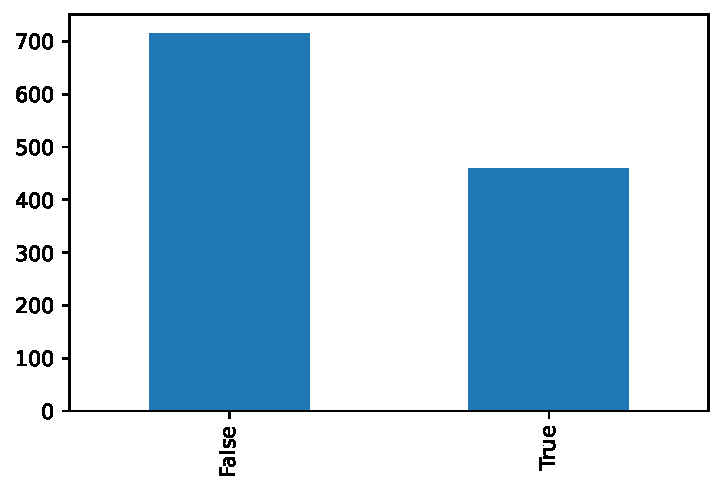
\includegraphics[keepaspectratio]{visualization_1/visualization_1_files/figure-pdf/cell-3-output-1.pdf}}

Recall that \texttt{.value\_counts()} returns a \texttt{Series} with the
total count of each unique value. We call
\texttt{.plot(kind=\textquotesingle{}bar\textquotesingle{})} on this
result to visualize these counts as a bar plot.

Plotting methods in \texttt{pandas} are the least preferred and not
supported in Data 100, as their functionality is limited. Instead,
future examples will focus on other libraries built specifically for
visualizing data. The most well-known library here is
\texttt{matplotlib}.

\subsection{Plotting in Matplotlib}\label{plotting-in-matplotlib}

\begin{Shaded}
\begin{Highlighting}[]
\ImportTok{import}\NormalTok{ matplotlib.pyplot }\ImportTok{as}\NormalTok{ plt }\CommentTok{\# matplotlib is typically given the alias plt}

\NormalTok{continent }\OperatorTok{=}\NormalTok{ wb[}\StringTok{\textquotesingle{}Continent\textquotesingle{}}\NormalTok{].value\_counts()}
\NormalTok{plt.bar(continent.index, continent)}
\NormalTok{plt.xlabel(}\StringTok{\textquotesingle{}Continent\textquotesingle{}}\NormalTok{)}
\NormalTok{plt.ylabel(}\StringTok{\textquotesingle{}Count\textquotesingle{}}\NormalTok{)}\OperatorTok{;}
\end{Highlighting}
\end{Shaded}

\pandocbounded{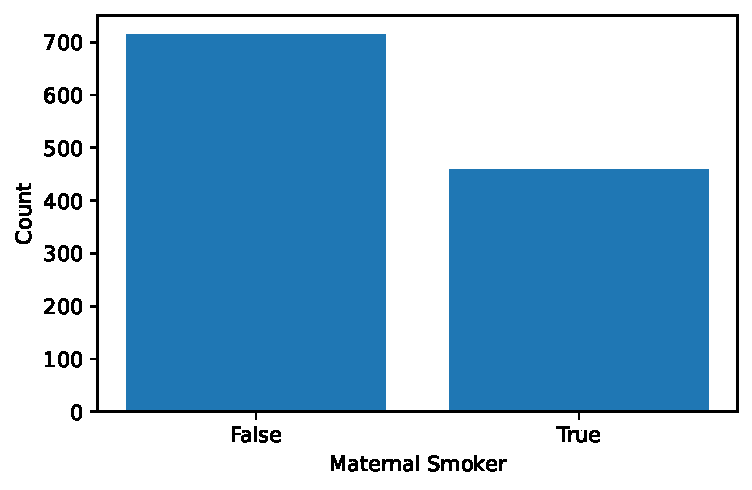
\includegraphics[keepaspectratio]{visualization_1/visualization_1_files/figure-pdf/cell-4-output-1.pdf}}

While more code is required to achieve the same result,
\texttt{matplotlib} is often used over \texttt{pandas} for its ability
to plot more complex visualizations, some of which are discussed
shortly.

However, note how we needed to label the axes with \texttt{plt.xlabel}
and \texttt{plt.ylabel}, as \texttt{matplotlib} does not support
automatic axis labeling. To get around these inconveniences, we can use
a more efficient plotting library: \texttt{seaborn}.

\subsection{\texorpdfstring{Plotting in
\texttt{Seaborn}}{Plotting in Seaborn}}\label{plotting-in-seaborn}

\begin{Shaded}
\begin{Highlighting}[]
\ImportTok{import}\NormalTok{ seaborn }\ImportTok{as}\NormalTok{ sns }\CommentTok{\# seaborn is typically given the alias sns}
\NormalTok{sns.countplot(data }\OperatorTok{=}\NormalTok{ wb, x }\OperatorTok{=} \StringTok{\textquotesingle{}Continent\textquotesingle{}}\NormalTok{)}\OperatorTok{;}
\end{Highlighting}
\end{Shaded}

\pandocbounded{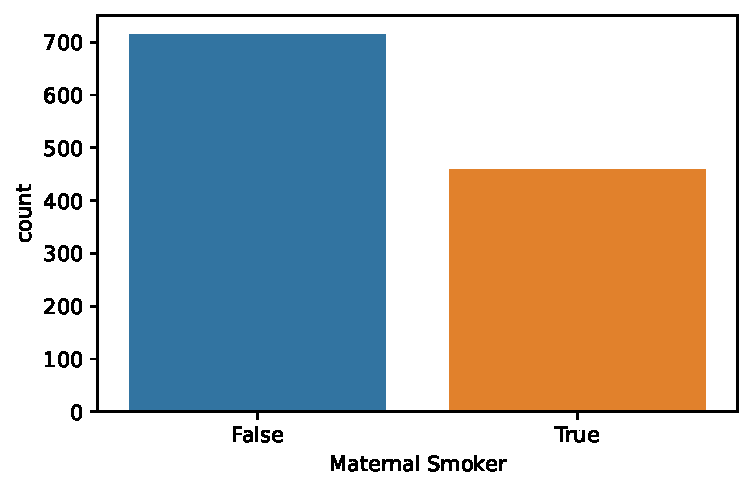
\includegraphics[keepaspectratio]{visualization_1/visualization_1_files/figure-pdf/cell-5-output-1.pdf}}

In contrast to \texttt{matplotlib}, the general structure of a
\texttt{seaborn} call involves passing in an entire \texttt{DataFrame},
and then specifying what column(s) to plot. \texttt{seaborn.countplot}
both counts and visualizes the number of unique values in a given
column. This column is specified by the \texttt{x} argument to
\texttt{sns.countplot}, while the \texttt{DataFrame} is specified by the
\texttt{data} argument.

\begin{quote}
\texttt{seaborn} is built on \texttt{matplotlib}! When using
\texttt{seaborn}, you're actually using \texttt{matplotlib} under the
hood, but with an easier-to-use interface for working with
\texttt{DataFrame}s and creating certain types of plots.
\end{quote}

For the vast majority of visualizations, \texttt{seaborn} is far more
concise and aesthetically pleasing than \texttt{matplotlib}. However,
the color scheme of this particular bar plot is arbitrary - it encodes
no additional information about the categories themselves. This is not
always true; color may signify meaningful detail in other
visualizations. We'll explore this more in-depth during the next
lecture.

By now, you'll have noticed that each of these plotting libraries have a
very different syntax. As with \texttt{pandas}, we'll teach you the
important methods in \texttt{matplotlib} and \texttt{seaborn}, but
you'll learn more through documentation.

\begin{enumerate}
\def\labelenumi{\arabic{enumi}.}
\tightlist
\item
  \href{https://matplotlib.org/stable/index.html}{Matplotlib
  Documentation}
\item
  \href{https://seaborn.pydata.org/}{Seaborn Documentation}
\end{enumerate}

\section{Distributions of Quantitative
Variables}\label{distributions-of-quantitative-variables}

Revisiting our example with the \texttt{wb} DataFrame, let's plot the
distribution of \texttt{Gross\ national\ income\ per\ capita}.

\begin{Shaded}
\begin{Highlighting}[]
\NormalTok{wb.head(}\DecValTok{5}\NormalTok{)}
\end{Highlighting}
\end{Shaded}

\begin{longtable}[]{@{}llllllllllllllllllllll@{}}
\toprule\noalign{}
& Continent & Country & Primary completion rate: Male: \% of relevant
age group: 2015 & Primary completion rate: Female: \% of relevant age
group: 2015 & Lower secondary completion rate: Male: \% of relevant age
group: 2015 & Lower secondary completion rate: Female: \% of relevant
age group: 2015 & Youth literacy rate: Male: \% of ages 15-24: 2005-14 &
Youth literacy rate: Female: \% of ages 15-24: 2005-14 & Adult literacy
rate: Male: \% ages 15 and older: 2005-14 & Adult literacy rate: Female:
\% ages 15 and older: 2005-14 & ... & Access to improved sanitation
facilities: \% of population: 1990 & Access to improved sanitation
facilities: \% of population: 2015 & Child immunization rate: Measles:
\% of children ages 12-23 months: 2015 & Child immunization rate: DTP3:
\% of children ages 12-23 months: 2015 & Children with acute respiratory
infection taken to health provider: \% of children under age 5 with ARI:
2009-2016 & Children with diarrhea who received oral rehydration and
continuous feeding: \% of children under age 5 with diarrhea: 2009-2016
& Children sleeping under treated bed nets: \% of children under age 5:
2009-2016 & Children with fever receiving antimalarial drugs: \% of
children under age 5 with fever: 2009-2016 & Tuberculosis: Treatment
success rate: \% of new cases: 2014 & Tuberculosis: Cases detection
rate: \% of new estimated cases: 2015 \\
\midrule\noalign{}
\endhead
\bottomrule\noalign{}
\endlastfoot
0 & Africa & Algeria & 106.0 & 105.0 & 68.0 & 85.0 & 96.0 & 92.0 & 83.0
& 68.0 & ... & 80.0 & 88.0 & 95.0 & 95.0 & 66.0 & 42.0 & NaN & NaN &
88.0 & 80.0 \\
1 & Africa & Angola & NaN & NaN & NaN & NaN & 79.0 & 67.0 & 82.0 & 60.0
& ... & 22.0 & 52.0 & 55.0 & 64.0 & NaN & NaN & 25.9 & 28.3 & 34.0 &
64.0 \\
2 & Africa & Benin & 83.0 & 73.0 & 50.0 & 37.0 & 55.0 & 31.0 & 41.0 &
18.0 & ... & 7.0 & 20.0 & 75.0 & 79.0 & 23.0 & 33.0 & 72.7 & 25.9 & 89.0
& 61.0 \\
3 & Africa & Botswana & 98.0 & 101.0 & 86.0 & 87.0 & 96.0 & 99.0 & 87.0
& 89.0 & ... & 39.0 & 63.0 & 97.0 & 95.0 & NaN & NaN & NaN & NaN & 77.0
& 62.0 \\
5 & Africa & Burundi & 58.0 & 66.0 & 35.0 & 30.0 & 90.0 & 88.0 & 89.0 &
85.0 & ... & 42.0 & 48.0 & 93.0 & 94.0 & 55.0 & 43.0 & 53.8 & 25.4 &
91.0 & 51.0 \\
\end{longtable}

How should we define our categories for this variable? In the previous
example, these were a few unique values of the \texttt{Continent}
column. If we use similar logic here, our categories are the different
numerical values contained in the
\texttt{Gross\ national\ income\ per\ capita} column.

Under this assumption, let's plot this distribution using the
\texttt{seaborn.countplot} function.

\begin{Shaded}
\begin{Highlighting}[]
\NormalTok{sns.countplot(data }\OperatorTok{=}\NormalTok{ wb, x }\OperatorTok{=} \StringTok{\textquotesingle{}Gross national income per capita, Atlas method: $: 2016\textquotesingle{}}\NormalTok{)}\OperatorTok{;}
\end{Highlighting}
\end{Shaded}

\pandocbounded{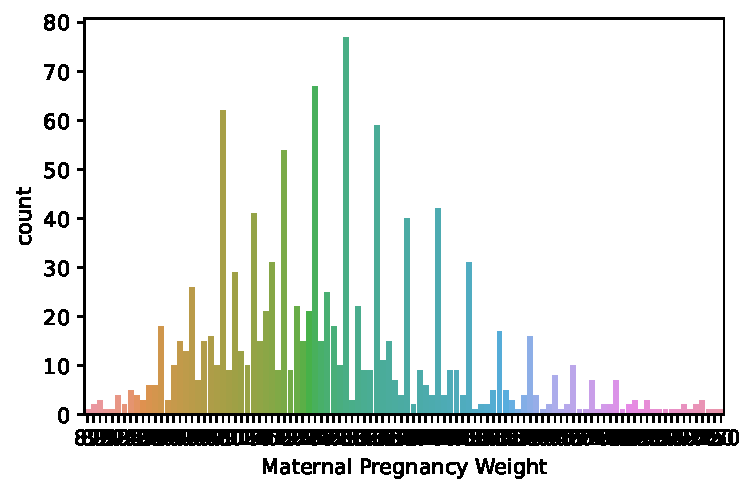
\includegraphics[keepaspectratio]{visualization_1/visualization_1_files/figure-pdf/cell-7-output-1.pdf}}

What happened? A bar plot (either \texttt{plt.bar} or
\texttt{sns.countplot}) will create a separate bar for each unique value
of a variable. With a continuous variable, we may not have a finite
number of possible values, which can lead to situations like above where
we would need many, many bars to display each unique value.

Specifically, we can say this histogram suffers from
\textbf{overplotting} as we are unable to interpret the plot and gain
any meaningful insight.

Rather than bar plots, to visualize the distribution of a continuous
variable, we use one of the following types of plots:

\begin{itemize}
\tightlist
\item
  Histogram
\item
  Box plot
\item
  Violin plot
\end{itemize}

\subsection{Box Plots and Violin
Plots}\label{box-plots-and-violin-plots}

Box plots and violin plots are two very similar kinds of visualizations.
Both display the distribution of a variable using information about
\textbf{quartiles}.

In a box plot, the width of the box at any point does not encode
meaning. In a violin plot, the width of the plot indicates the density
of the distribution at each possible value.

\begin{Shaded}
\begin{Highlighting}[]
\NormalTok{sns.boxplot(data}\OperatorTok{=}\NormalTok{wb, y}\OperatorTok{=}\StringTok{\textquotesingle{}Gross national income per capita, Atlas method: $: 2016\textquotesingle{}}\NormalTok{)}\OperatorTok{;}
\end{Highlighting}
\end{Shaded}

\pandocbounded{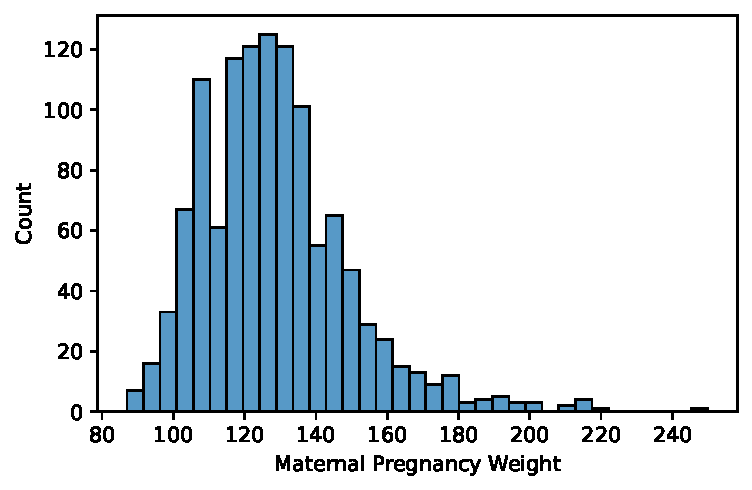
\includegraphics[keepaspectratio]{visualization_1/visualization_1_files/figure-pdf/cell-8-output-1.pdf}}

\begin{Shaded}
\begin{Highlighting}[]
\NormalTok{sns.violinplot(data}\OperatorTok{=}\NormalTok{wb, y}\OperatorTok{=}\StringTok{"Gross national income per capita, Atlas method: $: 2016"}\NormalTok{)}\OperatorTok{;}
\end{Highlighting}
\end{Shaded}

\pandocbounded{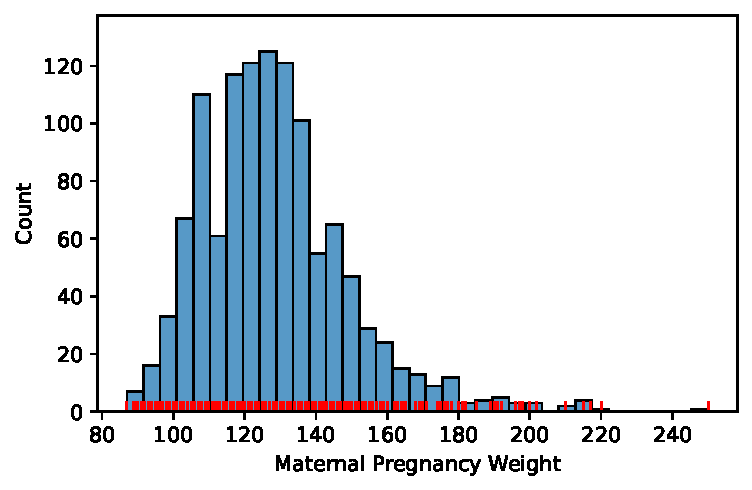
\includegraphics[keepaspectratio]{visualization_1/visualization_1_files/figure-pdf/cell-9-output-1.pdf}}

A quartile represents a 25\% portion of the data. We say that:

\begin{itemize}
\tightlist
\item
  The first quartile (Q1) represents the 25th percentile -- 25\% of the
  data is smaller than or equal to the first quartile.
\item
  The second quartile (Q2) represents the 50th percentile, also known as
  the median -- 50\% of the data is smaller than or equal to the second
  quartile.
\item
  The third quartile (Q3) represents the 75th percentile -- 75\% of the
  data is smaller than or equal to the third quartile.
\end{itemize}

This means that the middle 50\% of the data lies between the first and
third quartiles. This is demonstrated in the histogram below. The three
quartiles are marked with red vertical bars.

\begin{Shaded}
\begin{Highlighting}[]
\NormalTok{gdp }\OperatorTok{=}\NormalTok{ wb[}\StringTok{\textquotesingle{}Gross domestic product: }\SpecialCharTok{\% g}\StringTok{rowth : 2016\textquotesingle{}}\NormalTok{]}
\NormalTok{gdp }\OperatorTok{=}\NormalTok{ gdp[}\OperatorTok{\textasciitilde{}}\NormalTok{gdp.isna()]}

\NormalTok{q1, q2, q3 }\OperatorTok{=}\NormalTok{ np.percentile(gdp, [}\DecValTok{25}\NormalTok{, }\DecValTok{50}\NormalTok{, }\DecValTok{75}\NormalTok{])}

\NormalTok{wb\_quartiles }\OperatorTok{=}\NormalTok{ wb.copy()}
\NormalTok{wb\_quartiles[}\StringTok{\textquotesingle{}category\textquotesingle{}}\NormalTok{] }\OperatorTok{=} \VariableTok{None}
\NormalTok{wb\_quartiles.loc[(wb\_quartiles[}\StringTok{\textquotesingle{}Gross domestic product: }\SpecialCharTok{\% g}\StringTok{rowth : 2016\textquotesingle{}}\NormalTok{] }\OperatorTok{\textless{}}\NormalTok{ q1) }\OperatorTok{|}\NormalTok{ (wb\_quartiles[}\StringTok{\textquotesingle{}Gross domestic product: }\SpecialCharTok{\% g}\StringTok{rowth : 2016\textquotesingle{}}\NormalTok{] }\OperatorTok{\textgreater{}}\NormalTok{ q3), }\StringTok{\textquotesingle{}category\textquotesingle{}}\NormalTok{] }\OperatorTok{=} \StringTok{\textquotesingle{}Outside of the middle 50\%\textquotesingle{}}
\NormalTok{wb\_quartiles.loc[(wb\_quartiles[}\StringTok{\textquotesingle{}Gross domestic product: }\SpecialCharTok{\% g}\StringTok{rowth : 2016\textquotesingle{}}\NormalTok{] }\OperatorTok{\textgreater{}}\NormalTok{ q1) }\OperatorTok{\&}\NormalTok{ (wb\_quartiles[}\StringTok{\textquotesingle{}Gross domestic product: }\SpecialCharTok{\% g}\StringTok{rowth : 2016\textquotesingle{}}\NormalTok{] }\OperatorTok{\textless{}}\NormalTok{ q3), }\StringTok{\textquotesingle{}category\textquotesingle{}}\NormalTok{] }\OperatorTok{=} \StringTok{\textquotesingle{}In the middle 50\%\textquotesingle{}}

\NormalTok{sns.histplot(wb\_quartiles, x}\OperatorTok{=}\StringTok{"Gross domestic product: }\SpecialCharTok{\% g}\StringTok{rowth : 2016"}\NormalTok{, hue}\OperatorTok{=}\StringTok{"category"}\NormalTok{)}
\NormalTok{sns.rugplot([q1, q2, q3], c}\OperatorTok{=}\StringTok{"firebrick"}\NormalTok{, lw}\OperatorTok{=}\DecValTok{6}\NormalTok{, height}\OperatorTok{=}\FloatTok{0.1}\NormalTok{)}\OperatorTok{;}
\end{Highlighting}
\end{Shaded}

\pandocbounded{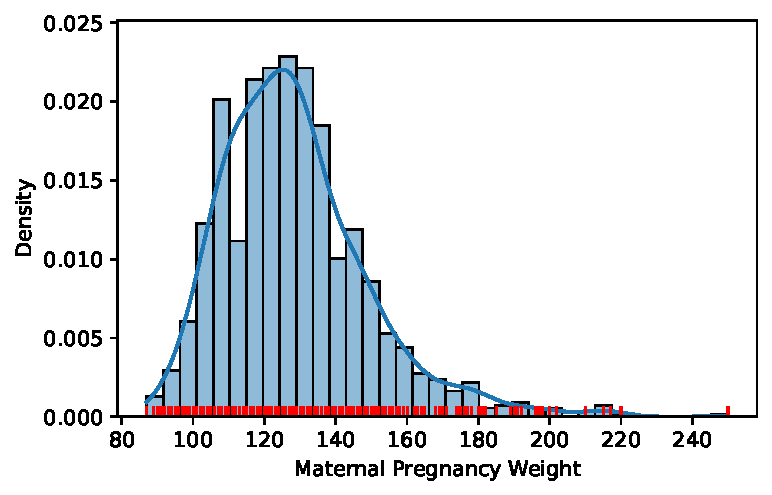
\includegraphics[keepaspectratio]{visualization_1/visualization_1_files/figure-pdf/cell-10-output-1.pdf}}

In a box plot, the lower extent of the box lies at Q1, while the upper
extent of the box lies at Q3. The horizontal line in the middle of the
box corresponds to Q2 (equivalently, the median).

\begin{Shaded}
\begin{Highlighting}[]
\NormalTok{sns.boxplot(data}\OperatorTok{=}\NormalTok{wb, y}\OperatorTok{=}\StringTok{\textquotesingle{}Gross domestic product: }\SpecialCharTok{\% g}\StringTok{rowth : 2016\textquotesingle{}}\NormalTok{)}\OperatorTok{;}
\end{Highlighting}
\end{Shaded}

\pandocbounded{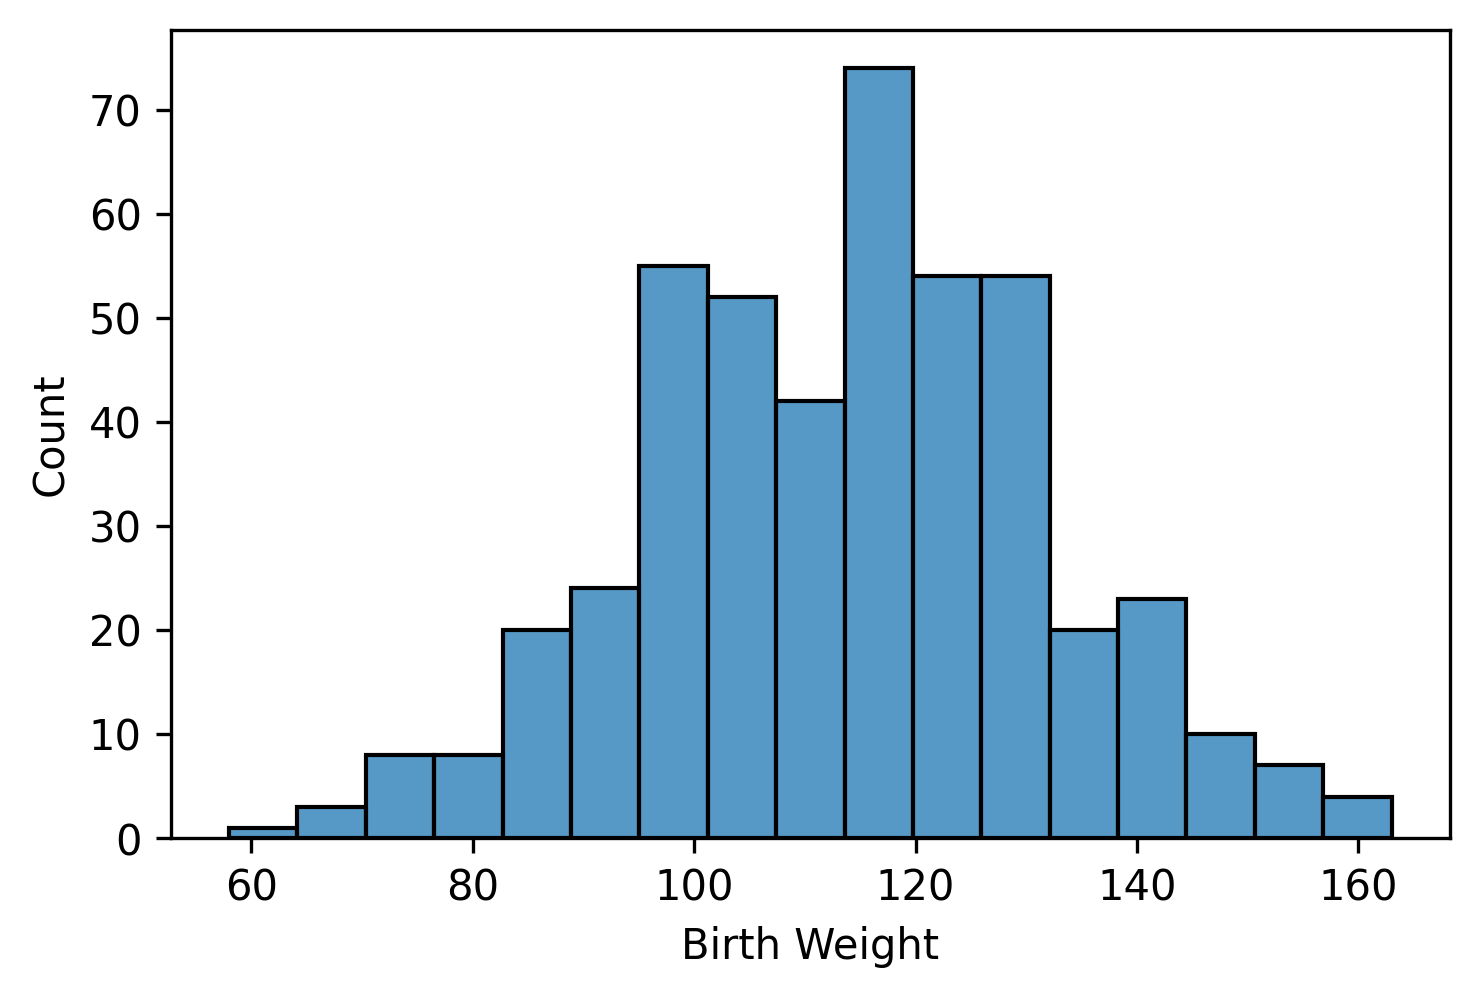
\includegraphics[keepaspectratio]{visualization_1/visualization_1_files/figure-pdf/cell-11-output-1.pdf}}

The \textbf{whiskers} of a box-plot are the two points that lie at the
{[}\(1^{st}\) Quartile \(-\) (\(1.5\times\) IQR){]}, and the
{[}\(3^{rd}\) Quartile \(+\) (\(1.5\times\) IQR){]}. They are the lower
and upper ranges of ``normal'' data (the points excluding outliers).

The different forms of information contained in a box plot can be
summarised as follows:

A violin plot displays quartile information, albeit a bit more subtly
through smoothed density curves. Look closely at the center vertical bar
of the violin plot below; the three quartiles and ``whiskers'' are still
present!

\begin{Shaded}
\begin{Highlighting}[]
\NormalTok{sns.violinplot(data}\OperatorTok{=}\NormalTok{wb, y}\OperatorTok{=}\StringTok{\textquotesingle{}Gross domestic product: }\SpecialCharTok{\% g}\StringTok{rowth : 2016\textquotesingle{}}\NormalTok{)}\OperatorTok{;}
\end{Highlighting}
\end{Shaded}

\pandocbounded{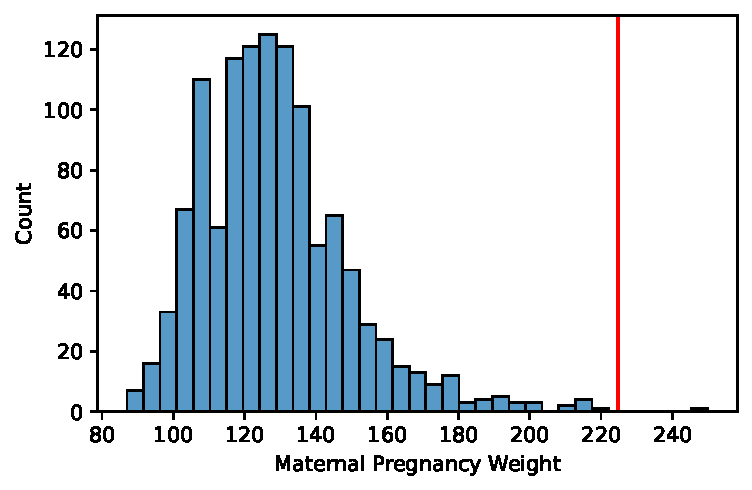
\includegraphics[keepaspectratio]{visualization_1/visualization_1_files/figure-pdf/cell-12-output-1.pdf}}

\subsection{Side-by-Side Box and Violin
Plots}\label{side-by-side-box-and-violin-plots}

Plotting side-by-side box or violin plots allows us to compare
distributions across different categories. In other words, they enable
us to plot both a qualitative variable and a quantitative continuous
variable in one visualization.

With \texttt{seaborn}, we can easily create side-by-side plots by
specifying both an x and y column.

\begin{Shaded}
\begin{Highlighting}[]
\NormalTok{sns.boxplot(data}\OperatorTok{=}\NormalTok{wb, x}\OperatorTok{=}\StringTok{"Continent"}\NormalTok{, y}\OperatorTok{=}\StringTok{\textquotesingle{}Gross domestic product: }\SpecialCharTok{\% g}\StringTok{rowth : 2016\textquotesingle{}}\NormalTok{)}\OperatorTok{;}
\end{Highlighting}
\end{Shaded}

\pandocbounded{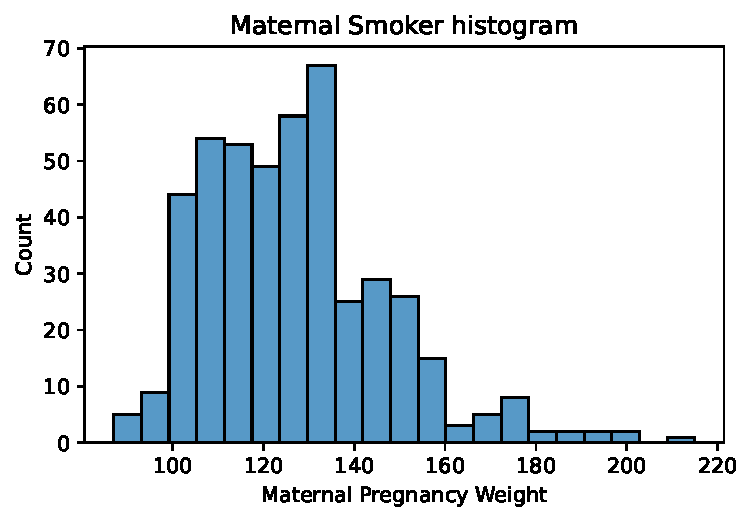
\includegraphics[keepaspectratio]{visualization_1/visualization_1_files/figure-pdf/cell-13-output-1.pdf}}

\subsection{Histograms}\label{histograms}

You are likely familiar with histograms from Data 8. A histogram
collects continuous data into bins, then plots this binned data. Each
bin reflects the density of datapoints with values that lie between the
left and right ends of the bin; in other words, the \textbf{area} of
each bin is proportional to the \textbf{percentage} of datapoints it
contains.

\subsubsection{Plotting Histograms}\label{plotting-histograms}

Below, we plot a histogram using matplotlib and seaborn. Which graph do
you prefer?

\begin{Shaded}
\begin{Highlighting}[]
\CommentTok{\# The \textasciigrave{}edgecolor\textasciigrave{} argument controls the color of the bin edges}
\NormalTok{gni }\OperatorTok{=}\NormalTok{ wb[}\StringTok{"Gross national income per capita, Atlas method: $: 2016"}\NormalTok{]}
\NormalTok{plt.hist(gni, density}\OperatorTok{=}\VariableTok{True}\NormalTok{, edgecolor}\OperatorTok{=}\StringTok{"white"}\NormalTok{)}

\CommentTok{\# Add labels}
\NormalTok{plt.xlabel(}\StringTok{"Gross national income per capita"}\NormalTok{)}
\NormalTok{plt.ylabel(}\StringTok{"Density"}\NormalTok{)}
\NormalTok{plt.title(}\StringTok{"Distribution of gross national income per capita"}\NormalTok{)}\OperatorTok{;}
\end{Highlighting}
\end{Shaded}

\pandocbounded{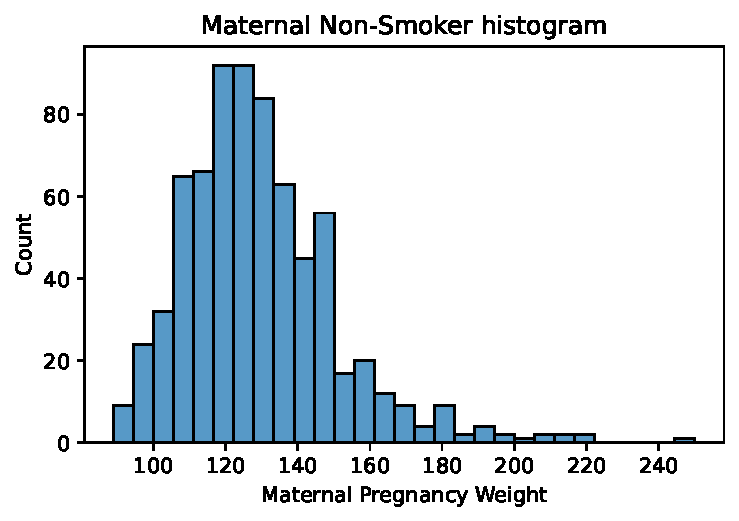
\includegraphics[keepaspectratio]{visualization_1/visualization_1_files/figure-pdf/cell-14-output-1.pdf}}

\begin{Shaded}
\begin{Highlighting}[]
\NormalTok{sns.histplot(data}\OperatorTok{=}\NormalTok{wb, x}\OperatorTok{=}\StringTok{"Gross national income per capita, Atlas method: $: 2016"}\NormalTok{, stat}\OperatorTok{=}\StringTok{"density"}\NormalTok{)}
\NormalTok{plt.title(}\StringTok{"Distribution of gross national income per capita"}\NormalTok{)}\OperatorTok{;}
\end{Highlighting}
\end{Shaded}

\pandocbounded{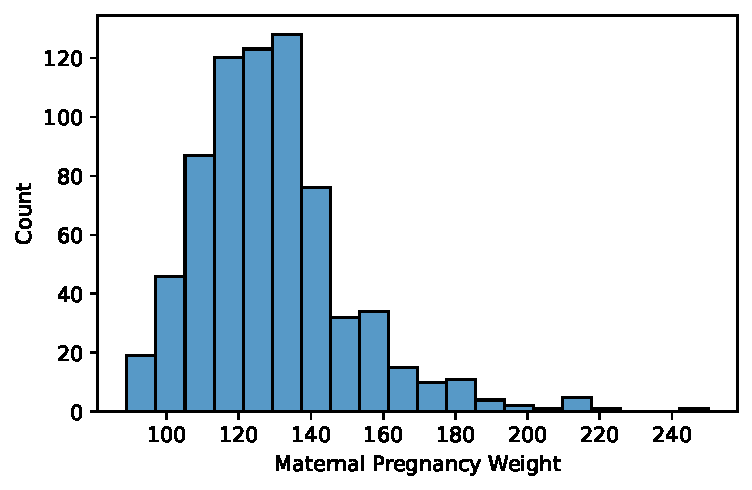
\includegraphics[keepaspectratio]{visualization_1/visualization_1_files/figure-pdf/cell-15-output-1.pdf}}

\subsubsection{Overlaid Histograms}\label{overlaid-histograms}

We can overlay histograms (or density curves) to compare distributions
across qualitative categories.

The \texttt{hue} parameter of \texttt{sns.histplot} specifies the column
that should be used to determine the color of each category.
\texttt{hue} can be used in many \texttt{seaborn} plotting functions.

Notice that the resulting plot includes a legend describing which color
corresponds to each hemisphere -- a legend should always be included if
color is used to encode information in a visualization!

\begin{Shaded}
\begin{Highlighting}[]
\CommentTok{\# Create a new variable to store the hemisphere in which each country is located}
\NormalTok{north }\OperatorTok{=}\NormalTok{ [}\StringTok{"Asia"}\NormalTok{, }\StringTok{"Europe"}\NormalTok{, }\StringTok{"N. America"}\NormalTok{]}
\NormalTok{south }\OperatorTok{=}\NormalTok{ [}\StringTok{"Africa"}\NormalTok{, }\StringTok{"Oceania"}\NormalTok{, }\StringTok{"S. America"}\NormalTok{]}
\NormalTok{wb.loc[wb[}\StringTok{"Continent"}\NormalTok{].isin(north), }\StringTok{"Hemisphere"}\NormalTok{] }\OperatorTok{=} \StringTok{"Northern"}
\NormalTok{wb.loc[wb[}\StringTok{"Continent"}\NormalTok{].isin(south), }\StringTok{"Hemisphere"}\NormalTok{] }\OperatorTok{=} \StringTok{"Southern"}
\end{Highlighting}
\end{Shaded}

\begin{Shaded}
\begin{Highlighting}[]
\NormalTok{sns.histplot(data}\OperatorTok{=}\NormalTok{wb, x}\OperatorTok{=}\StringTok{"Gross national income per capita, Atlas method: $: 2016"}\NormalTok{, hue}\OperatorTok{=}\StringTok{"Hemisphere"}\NormalTok{, stat}\OperatorTok{=}\StringTok{"density"}\NormalTok{)}
\NormalTok{plt.title(}\StringTok{"Distribution of gross national income per capita"}\NormalTok{)}\OperatorTok{;}
\end{Highlighting}
\end{Shaded}

\pandocbounded{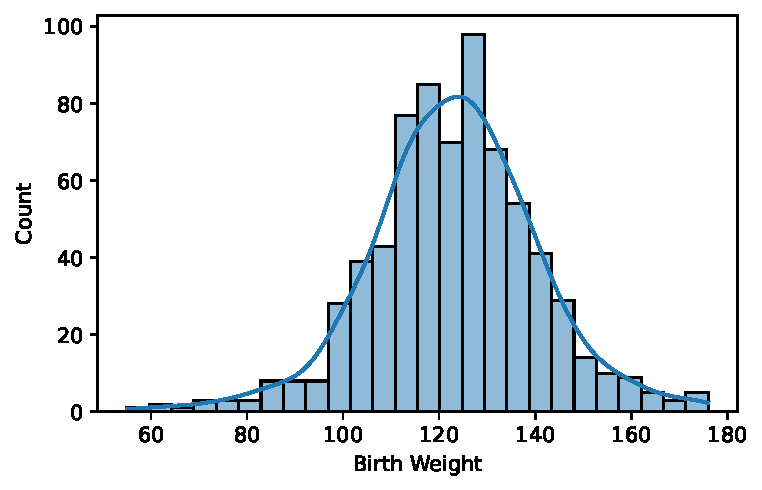
\includegraphics[keepaspectratio]{visualization_1/visualization_1_files/figure-pdf/cell-17-output-1.pdf}}

Again, each bin of a histogram is scaled such that its \textbf{area} is
proportional to the \textbf{percentage} of all datapoints that it
contains.

\begin{Shaded}
\begin{Highlighting}[]
\NormalTok{densities, bins, \_ }\OperatorTok{=}\NormalTok{ plt.hist(gni, density}\OperatorTok{=}\VariableTok{True}\NormalTok{, edgecolor}\OperatorTok{=}\StringTok{"white"}\NormalTok{, bins}\OperatorTok{=}\DecValTok{5}\NormalTok{)}
\NormalTok{plt.xlabel(}\StringTok{"Gross national income per capita"}\NormalTok{)}
\NormalTok{plt.ylabel(}\StringTok{"Density"}\NormalTok{)}

\BuiltInTok{print}\NormalTok{(}\SpecialStringTok{f"First bin has width }\SpecialCharTok{\{}\NormalTok{bins[}\DecValTok{1}\NormalTok{]}\OperatorTok{{-}}\NormalTok{bins[}\DecValTok{0}\NormalTok{]}\SpecialCharTok{\}}\SpecialStringTok{ and height }\SpecialCharTok{\{}\NormalTok{densities[}\DecValTok{0}\NormalTok{]}\SpecialCharTok{\}}\SpecialStringTok{"}\NormalTok{)}
\BuiltInTok{print}\NormalTok{(}\SpecialStringTok{f"This corresponds to }\SpecialCharTok{\{}\NormalTok{bins[}\DecValTok{1}\NormalTok{]}\OperatorTok{{-}}\NormalTok{bins[}\DecValTok{0}\NormalTok{]}\SpecialCharTok{\}}\SpecialStringTok{ * }\SpecialCharTok{\{}\NormalTok{densities[}\DecValTok{0}\NormalTok{]}\SpecialCharTok{\}}\SpecialStringTok{ = }\SpecialCharTok{\{}\NormalTok{(bins[}\DecValTok{1}\NormalTok{]}\OperatorTok{{-}}\NormalTok{bins[}\DecValTok{0}\NormalTok{])}\OperatorTok{*}\NormalTok{densities[}\DecValTok{0}\NormalTok{]}\OperatorTok{*}\DecValTok{100}\SpecialCharTok{\}}\SpecialStringTok{\% of the data"}\NormalTok{)}
\end{Highlighting}
\end{Shaded}

\begin{verbatim}
First bin has width 16410.0 and height 4.7741589911386953e-05
This corresponds to 16410.0 * 4.7741589911386953e-05 = 78.343949044586% of the data
\end{verbatim}

\pandocbounded{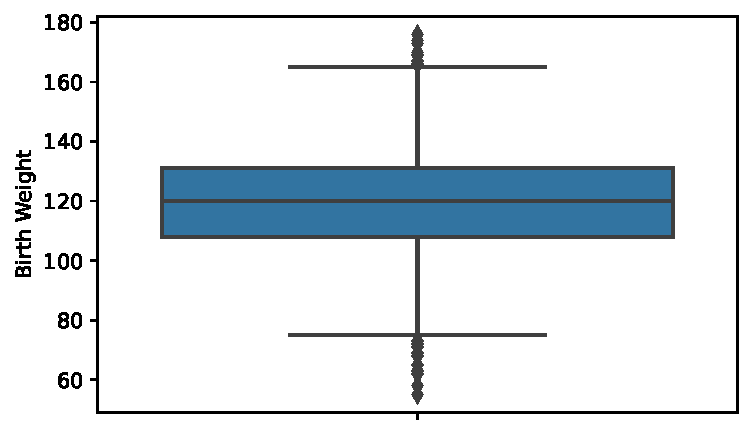
\includegraphics[keepaspectratio]{visualization_1/visualization_1_files/figure-pdf/cell-18-output-2.pdf}}

\subsubsection{Evaluating Histograms}\label{evaluating-histograms}

Histograms allow us to assess a distribution by their shape. There are a
few properties of histograms we can analyze:

\begin{enumerate}
\def\labelenumi{\arabic{enumi}.}
\tightlist
\item
  Skewness and Tails

  \begin{itemize}
  \tightlist
  \item
    Skewed left vs skewed right
  \item
    Left tail vs right tail
  \end{itemize}
\item
  Outliers

  \begin{itemize}
  \tightlist
  \item
    Using percentiles
  \end{itemize}
\item
  Modes

  \begin{itemize}
  \tightlist
  \item
    Most commonly occuring data
  \end{itemize}
\end{enumerate}

\paragraph{Skewness and Tails}\label{skewness-and-tails}

The skew of a histogram describes the direction in which its ``tail''
extends. - A distribution with a long right tail is \textbf{skewed
right} (such as \texttt{Gross\ national\ income\ per\ capita}). In a
right-skewed distribution, the few large outliers ``pull'' the mean to
the \textbf{right} of the median.

\begin{Shaded}
\begin{Highlighting}[]
\NormalTok{sns.histplot(data }\OperatorTok{=}\NormalTok{ wb, x }\OperatorTok{=} \StringTok{\textquotesingle{}Gross national income per capita, Atlas method: $: 2016\textquotesingle{}}\NormalTok{, stat }\OperatorTok{=} \StringTok{\textquotesingle{}density\textquotesingle{}}\NormalTok{)}\OperatorTok{;}
\NormalTok{plt.title(}\StringTok{\textquotesingle{}Distribution with a long right tail\textquotesingle{}}\NormalTok{)}
\end{Highlighting}
\end{Shaded}

\begin{verbatim}
Text(0.5, 1.0, 'Distribution with a long right tail')
\end{verbatim}

\pandocbounded{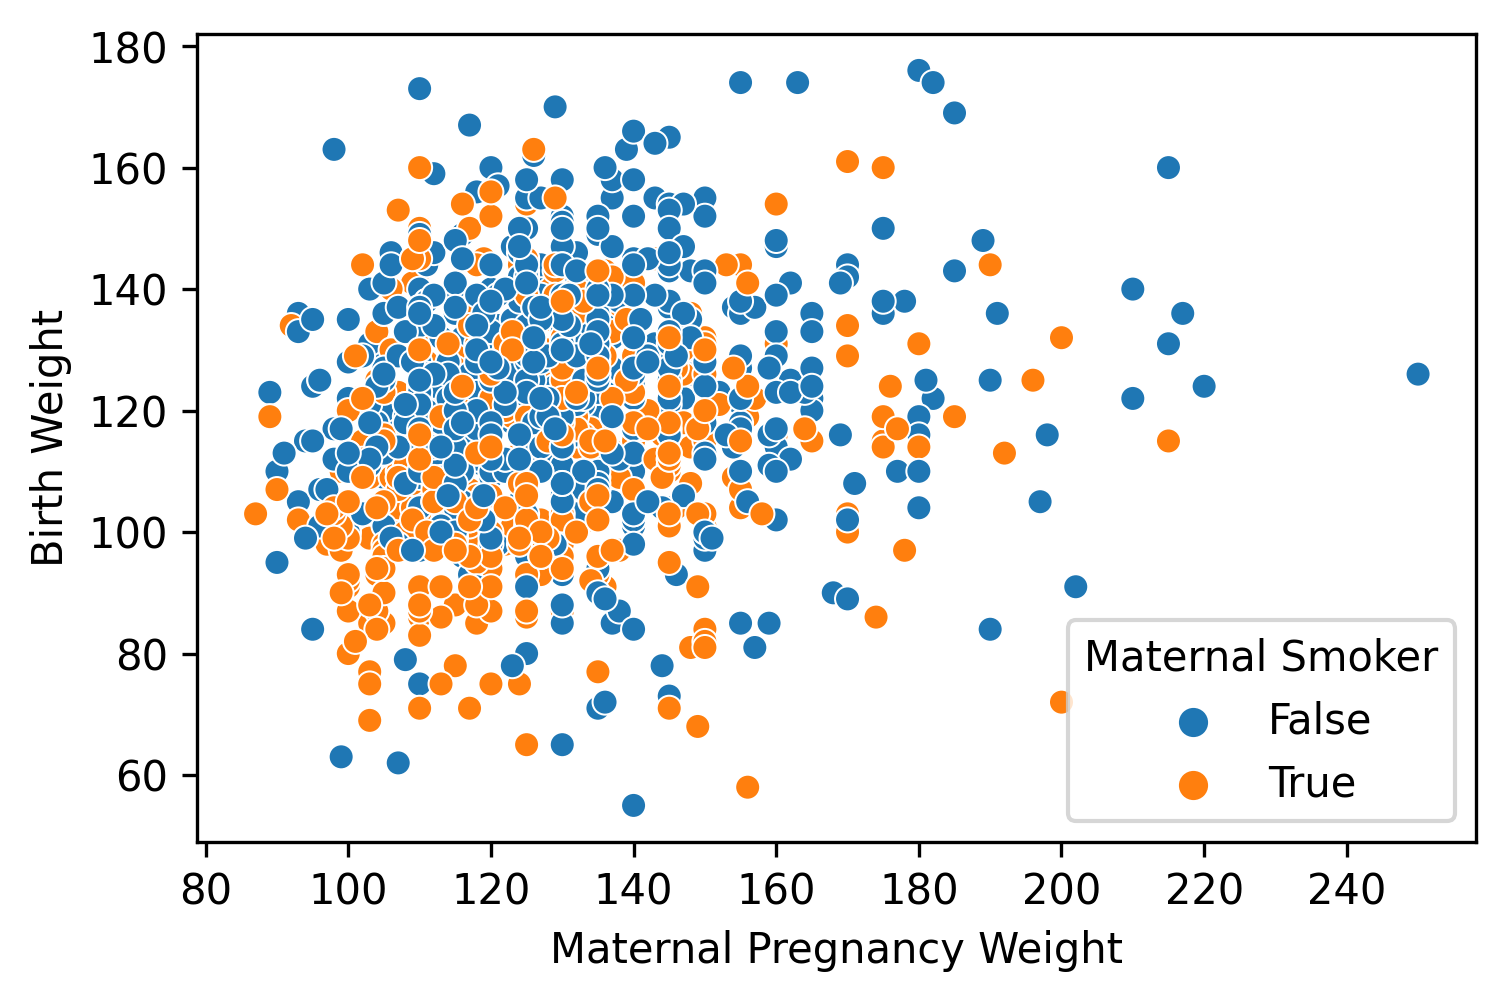
\includegraphics[keepaspectratio]{visualization_1/visualization_1_files/figure-pdf/cell-19-output-2.pdf}}

\begin{itemize}
\tightlist
\item
  A distribution with a long left tail is \textbf{skewed left} (such as
  \texttt{Access\ to\ an\ improved\ water\ source}). In a left-skewed
  distribution, the few small outliers ``pull'' the mean to the
  \textbf{left} of the median.
\end{itemize}

In the case where a distribution has equal-sized right and left tails,
it is \textbf{symmetric}. The mean is approximately \textbf{equal} to
the median. Think of mean as the balancing point of the distribution.

\begin{Shaded}
\begin{Highlighting}[]
\NormalTok{sns.histplot(data }\OperatorTok{=}\NormalTok{ wb, x }\OperatorTok{=} \StringTok{\textquotesingle{}Access to an improved water source: }\SpecialCharTok{\% o}\StringTok{f population: 2015\textquotesingle{}}\NormalTok{, stat }\OperatorTok{=} \StringTok{\textquotesingle{}density\textquotesingle{}}\NormalTok{)}\OperatorTok{;}
\NormalTok{plt.title(}\StringTok{\textquotesingle{}Distribution with a long left tail\textquotesingle{}}\NormalTok{)}
\end{Highlighting}
\end{Shaded}

\begin{verbatim}
Text(0.5, 1.0, 'Distribution with a long left tail')
\end{verbatim}

\pandocbounded{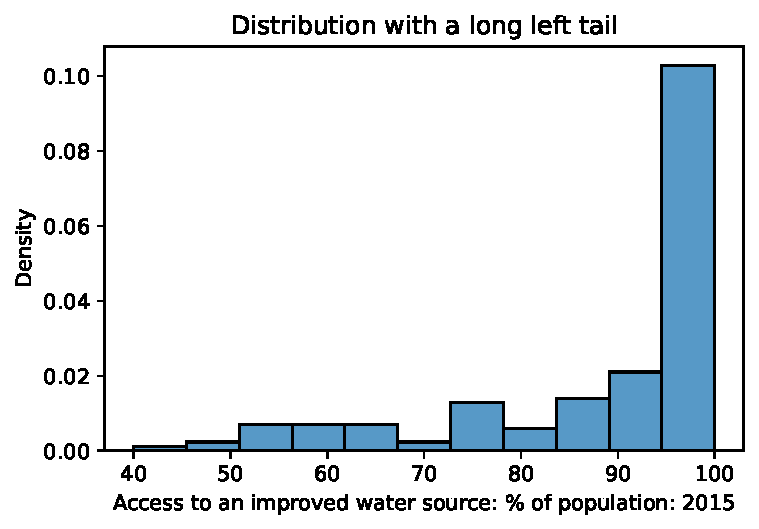
\includegraphics[keepaspectratio]{visualization_1/visualization_1_files/figure-pdf/cell-20-output-2.pdf}}

\paragraph{Outliers}\label{outliers}

Loosely speaking, an \textbf{outlier} is defined as a data point that
lies an abnormally large distance away from other values. Let's make
this more concrete. As you may have observed in the box plot infographic
earlier, we define \textbf{outliers} to be the data points that fall
beyond the whiskers. Specifically, values that are less than the
{[}\(1^{st}\) Quartile \(-\) (\(1.5\times\) IQR){]}, or greater than
{[}\(3^{rd}\) Quartile \(+\) (\(1.5\times\) IQR).{]}

\paragraph{Modes}\label{modes}

In Data 100, we describe a ``mode'' of a histogram as a peak in the
distribution. Often, however, it is difficult to determine what counts
as its own ``peak.'' For example, the number of peaks in the
distribution of HIV rates across different countries varies depending on
the number of histogram bins we plot.

If we set the number of bins to 5, the distribution appears unimodal.

\begin{Shaded}
\begin{Highlighting}[]
\CommentTok{\# Rename the very long column name for convenience}
\NormalTok{wb }\OperatorTok{=}\NormalTok{ wb.rename(columns}\OperatorTok{=}\NormalTok{\{}\StringTok{\textquotesingle{}Antiretroviral therapy coverage: }\SpecialCharTok{\% o}\StringTok{f people living with HIV: 2015\textquotesingle{}}\NormalTok{:}\StringTok{"HIV rate"}\NormalTok{\})}
\CommentTok{\# With 5 bins, it seems that there is only one peak}
\NormalTok{sns.histplot(data}\OperatorTok{=}\NormalTok{wb, x}\OperatorTok{=}\StringTok{"HIV rate"}\NormalTok{, stat}\OperatorTok{=}\StringTok{"density"}\NormalTok{, bins}\OperatorTok{=}\DecValTok{5}\NormalTok{)}
\NormalTok{plt.title(}\StringTok{"5 histogram bins"}\NormalTok{)}\OperatorTok{;}
\end{Highlighting}
\end{Shaded}

\pandocbounded{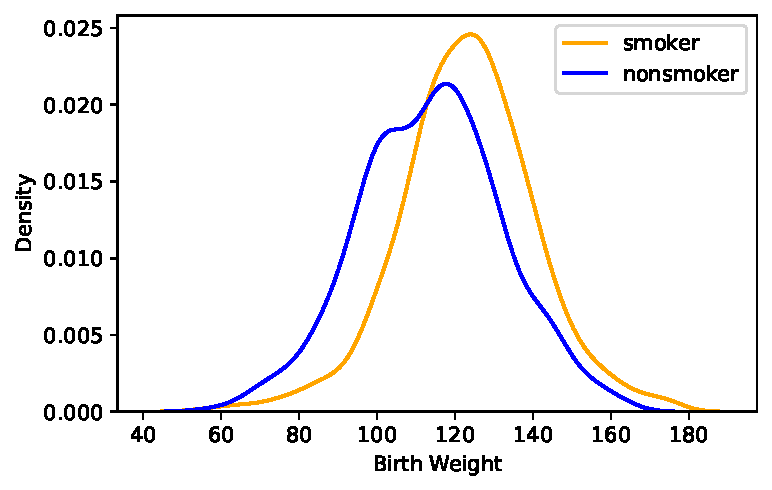
\includegraphics[keepaspectratio]{visualization_1/visualization_1_files/figure-pdf/cell-21-output-1.pdf}}

\begin{Shaded}
\begin{Highlighting}[]
\CommentTok{\# With 10 bins, there seem to be two peaks}

\NormalTok{sns.histplot(data}\OperatorTok{=}\NormalTok{wb, x}\OperatorTok{=}\StringTok{"HIV rate"}\NormalTok{, stat}\OperatorTok{=}\StringTok{"density"}\NormalTok{, bins}\OperatorTok{=}\DecValTok{10}\NormalTok{)}
\NormalTok{plt.title(}\StringTok{"10 histogram bins"}\NormalTok{)}\OperatorTok{;}
\end{Highlighting}
\end{Shaded}

\pandocbounded{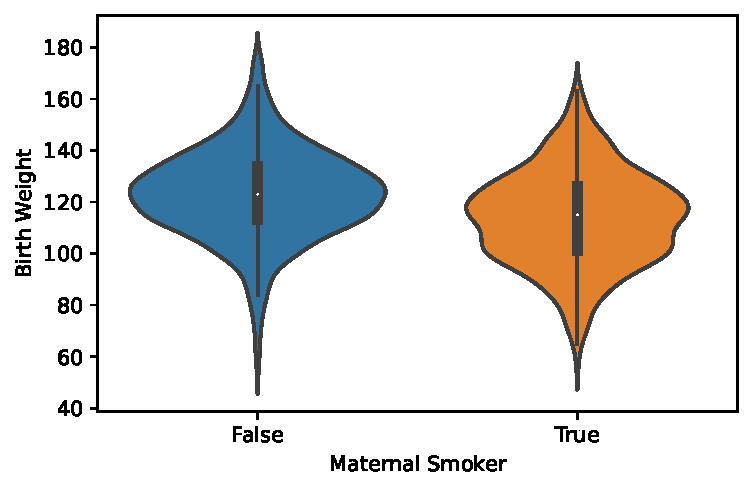
\includegraphics[keepaspectratio]{visualization_1/visualization_1_files/figure-pdf/cell-22-output-1.pdf}}

\begin{Shaded}
\begin{Highlighting}[]
\CommentTok{\# And with 20 bins, it becomes hard to say what counts as a "peak"!}

\NormalTok{sns.histplot(data}\OperatorTok{=}\NormalTok{wb, x }\OperatorTok{=}\StringTok{"HIV rate"}\NormalTok{, stat}\OperatorTok{=}\StringTok{"density"}\NormalTok{, bins}\OperatorTok{=}\DecValTok{20}\NormalTok{)}
\NormalTok{plt.title(}\StringTok{"20 histogram bins"}\NormalTok{)}\OperatorTok{;}
\end{Highlighting}
\end{Shaded}

\pandocbounded{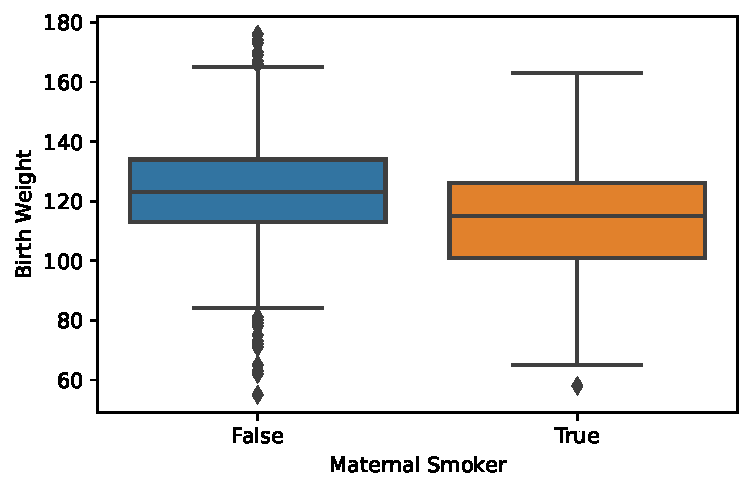
\includegraphics[keepaspectratio]{visualization_1/visualization_1_files/figure-pdf/cell-23-output-1.pdf}}

In part, it is these ambiguities that motivate us to consider using
Kernel Density Estimation (KDE), which we will explore more in the next
lecture.

\bookmarksetup{startatroot}

\chapter{Visualization II}\label{visualization-ii}

\begin{tcolorbox}[enhanced jigsaw, bottomrule=.15mm, coltitle=black, breakable, opacitybacktitle=0.6, leftrule=.75mm, bottomtitle=1mm, arc=.35mm, colback=white, toptitle=1mm, left=2mm, titlerule=0mm, title=\textcolor{quarto-callout-note-color}{\faInfo}\hspace{0.5em}{Learning Outcomes}, colframe=quarto-callout-note-color-frame, rightrule=.15mm, opacityback=0, toprule=.15mm, colbacktitle=quarto-callout-note-color!10!white]

\begin{itemize}
\tightlist
\item
  Understanding KDE for plotting distributions and estimating density
  curves.
\item
  Using transformations to analyze the relationship between two
  variables.
\item
  Evaluating the quality of a visualization based on visualization
  theory concepts.
\end{itemize}

\end{tcolorbox}

\section{Kernel Density Estimation}\label{kernel-density-estimation}

Often, we want to identify general trends across a distribution, rather
than focus on detail. Smoothing a distribution helps generalize the
structure of the data and eliminate noise.

\subsection{KDE Theory}\label{kde-theory}

A \textbf{kernel density estimate (KDE)} is a smooth, continuous
function that approximates a curve. It allows us to represent general
trends in a distribution without focusing on the details, which is
useful for analyzing the broad structure of a dataset.

More formally, a KDE attempts to approximate the underlying
\textbf{probability distribution} from which our dataset was drawn. You
may have encountered the idea of a probability distribution in your
other classes; if not, we'll discuss it at length in the next lecture.
For now, you can think of a probability distribution as a description of
how likely it is for us to sample a particular value in our dataset.

A KDE curve estimates the probability density function of a random
variable. Consider the example below, where we have used
\texttt{sns.displot} to plot both a histogram (containing the data
points we actually collected) and a KDE curve (representing the
\emph{approximated} probability distribution from which this data was
drawn) using data from the World Bank dataset (\texttt{wb}).

\begin{Shaded}
\begin{Highlighting}[]
\ImportTok{import}\NormalTok{ pandas }\ImportTok{as}\NormalTok{ pd}
\ImportTok{import}\NormalTok{ numpy }\ImportTok{as}\NormalTok{ np}
\ImportTok{import}\NormalTok{ matplotlib.pyplot }\ImportTok{as}\NormalTok{ plt}
\ImportTok{import}\NormalTok{ seaborn }\ImportTok{as}\NormalTok{ sns}
\ImportTok{import}\NormalTok{ warnings }

\NormalTok{warnings.filterwarnings(}\StringTok{"ignore"}\NormalTok{, }\StringTok{"use\_inf\_as\_na"}\NormalTok{) }\CommentTok{\# Supresses distracting deprecation warnings}

\NormalTok{wb }\OperatorTok{=}\NormalTok{ pd.read\_csv(}\StringTok{"data/world\_bank.csv"}\NormalTok{, index\_col}\OperatorTok{=}\DecValTok{0}\NormalTok{)}
\NormalTok{wb }\OperatorTok{=}\NormalTok{ wb.rename(columns}\OperatorTok{=}\NormalTok{\{}\StringTok{\textquotesingle{}Antiretroviral therapy coverage: }\SpecialCharTok{\% o}\StringTok{f people living with HIV: 2015\textquotesingle{}}\NormalTok{:}\StringTok{"HIV rate"}\NormalTok{,}
                       \StringTok{\textquotesingle{}Gross national income per capita, Atlas method: $: 2016\textquotesingle{}}\NormalTok{:}\StringTok{\textquotesingle{}gni\textquotesingle{}}\NormalTok{\})}
\NormalTok{wb.head()}
\end{Highlighting}
\end{Shaded}

\begin{longtable}[]{@{}llllllllllllllllllllll@{}}
\toprule\noalign{}
& Continent & Country & Primary completion rate: Male: \% of relevant
age group: 2015 & Primary completion rate: Female: \% of relevant age
group: 2015 & Lower secondary completion rate: Male: \% of relevant age
group: 2015 & Lower secondary completion rate: Female: \% of relevant
age group: 2015 & Youth literacy rate: Male: \% of ages 15-24: 2005-14 &
Youth literacy rate: Female: \% of ages 15-24: 2005-14 & Adult literacy
rate: Male: \% ages 15 and older: 2005-14 & Adult literacy rate: Female:
\% ages 15 and older: 2005-14 & ... & Access to improved sanitation
facilities: \% of population: 1990 & Access to improved sanitation
facilities: \% of population: 2015 & Child immunization rate: Measles:
\% of children ages 12-23 months: 2015 & Child immunization rate: DTP3:
\% of children ages 12-23 months: 2015 & Children with acute respiratory
infection taken to health provider: \% of children under age 5 with ARI:
2009-2016 & Children with diarrhea who received oral rehydration and
continuous feeding: \% of children under age 5 with diarrhea: 2009-2016
& Children sleeping under treated bed nets: \% of children under age 5:
2009-2016 & Children with fever receiving antimalarial drugs: \% of
children under age 5 with fever: 2009-2016 & Tuberculosis: Treatment
success rate: \% of new cases: 2014 & Tuberculosis: Cases detection
rate: \% of new estimated cases: 2015 \\
\midrule\noalign{}
\endhead
\bottomrule\noalign{}
\endlastfoot
0 & Africa & Algeria & 106.0 & 105.0 & 68.0 & 85.0 & 96.0 & 92.0 & 83.0
& 68.0 & ... & 80.0 & 88.0 & 95.0 & 95.0 & 66.0 & 42.0 & NaN & NaN &
88.0 & 80.0 \\
1 & Africa & Angola & NaN & NaN & NaN & NaN & 79.0 & 67.0 & 82.0 & 60.0
& ... & 22.0 & 52.0 & 55.0 & 64.0 & NaN & NaN & 25.9 & 28.3 & 34.0 &
64.0 \\
2 & Africa & Benin & 83.0 & 73.0 & 50.0 & 37.0 & 55.0 & 31.0 & 41.0 &
18.0 & ... & 7.0 & 20.0 & 75.0 & 79.0 & 23.0 & 33.0 & 72.7 & 25.9 & 89.0
& 61.0 \\
3 & Africa & Botswana & 98.0 & 101.0 & 86.0 & 87.0 & 96.0 & 99.0 & 87.0
& 89.0 & ... & 39.0 & 63.0 & 97.0 & 95.0 & NaN & NaN & NaN & NaN & 77.0
& 62.0 \\
5 & Africa & Burundi & 58.0 & 66.0 & 35.0 & 30.0 & 90.0 & 88.0 & 89.0 &
85.0 & ... & 42.0 & 48.0 & 93.0 & 94.0 & 55.0 & 43.0 & 53.8 & 25.4 &
91.0 & 51.0 \\
\end{longtable}

\begin{Shaded}
\begin{Highlighting}[]
\ImportTok{import}\NormalTok{ seaborn }\ImportTok{as}\NormalTok{ sns}
\ImportTok{import}\NormalTok{ matplotlib.pyplot }\ImportTok{as}\NormalTok{ plt}

\NormalTok{sns.displot(data }\OperatorTok{=}\NormalTok{ wb, x }\OperatorTok{=} \StringTok{\textquotesingle{}HIV rate\textquotesingle{}}\NormalTok{, }\OperatorTok{\textbackslash{}}
\NormalTok{                       kde }\OperatorTok{=} \VariableTok{True}\NormalTok{, stat }\OperatorTok{=} \StringTok{"density"}\NormalTok{)}

\NormalTok{plt.title(}\StringTok{"Distribution of HIV rates"}\NormalTok{)}\OperatorTok{;}
\end{Highlighting}
\end{Shaded}

\pandocbounded{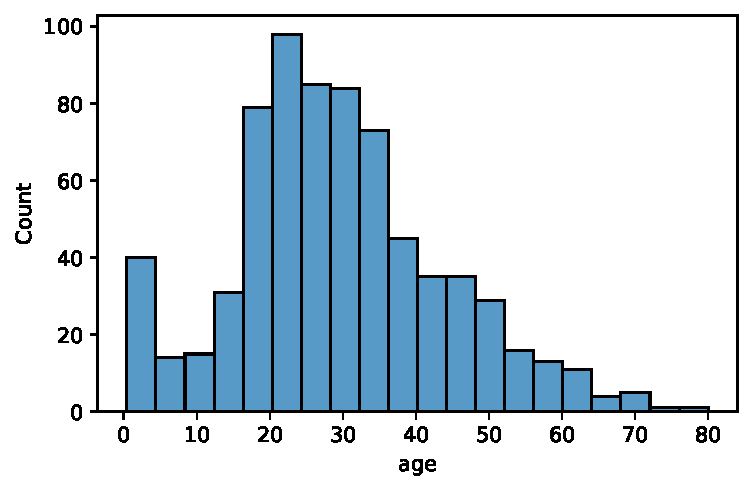
\includegraphics[keepaspectratio]{visualization_2/visualization_2_files/figure-pdf/cell-3-output-1.pdf}}

Notice that the smooth KDE curve is higher when the histogram bins are
taller. You can think of the height of the KDE curve as representing how
``probable'' it is that we randomly sample a datapoint with the
corresponding value. This intuitively makes sense -- if we have already
collected more datapoints with a particular value (resulting in a tall
histogram bin), it is more likely that, if we randomly sample another
datapoint, we will sample one with a similar value (resulting in a high
KDE curve).

The area under a probability density function should always integrate to
1, representing the fact that the total probability of a distribution
should always sum to 100\%. Hence, a KDE curve will always have an area
under the curve of 1.

\subsection{Constructing a KDE}\label{constructing-a-kde}

We perform kernel density estimation using three steps.

\begin{enumerate}
\def\labelenumi{\arabic{enumi}.}
\tightlist
\item
  Place a kernel at each datapoint.
\item
  Normalize the kernels to have a total area of 1 (across all kernels).
\item
  Sum the normalized kernels.
\end{enumerate}

We'll explain what a ``kernel'' is momentarily.

To make things simpler, let's construct a KDE for a small, artificially
generated dataset of 5 datapoints: \([2.2, 2.8, 3.7, 5.3, 5.7]\). In the
plot below, each vertical bar represents one data point.

\begin{Shaded}
\begin{Highlighting}[]
\NormalTok{data }\OperatorTok{=}\NormalTok{ [}\FloatTok{2.2}\NormalTok{, }\FloatTok{2.8}\NormalTok{, }\FloatTok{3.7}\NormalTok{, }\FloatTok{5.3}\NormalTok{, }\FloatTok{5.7}\NormalTok{]}

\NormalTok{sns.rugplot(data, height}\OperatorTok{=}\FloatTok{0.3}\NormalTok{)}

\NormalTok{plt.xlabel(}\StringTok{"Data"}\NormalTok{)}
\NormalTok{plt.ylabel(}\StringTok{"Density"}\NormalTok{)}
\NormalTok{plt.xlim(}\OperatorTok{{-}}\DecValTok{3}\NormalTok{, }\DecValTok{10}\NormalTok{)}
\NormalTok{plt.ylim(}\DecValTok{0}\NormalTok{, }\FloatTok{0.5}\NormalTok{)}\OperatorTok{;}
\end{Highlighting}
\end{Shaded}

\pandocbounded{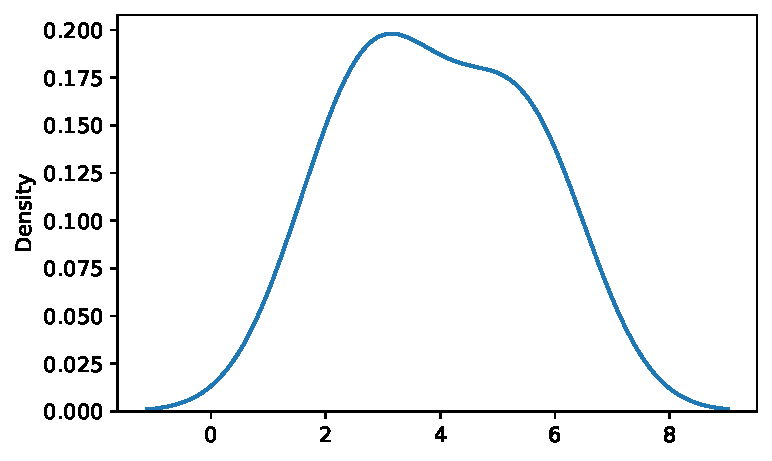
\includegraphics[keepaspectratio]{visualization_2/visualization_2_files/figure-pdf/cell-4-output-1.pdf}}

Our goal is to create the following KDE curve, which was generated
automatically by \texttt{sns.kdeplot}.

\begin{Shaded}
\begin{Highlighting}[]
\NormalTok{plt.xlabel(}\StringTok{"Data"}\NormalTok{)}
\NormalTok{plt.xlim(}\OperatorTok{{-}}\DecValTok{3}\NormalTok{, }\DecValTok{10}\NormalTok{)}
\NormalTok{plt.ylim(}\DecValTok{0}\NormalTok{, }\FloatTok{0.5}\NormalTok{)}

\NormalTok{sns.kdeplot(data, bw\_method}\OperatorTok{=}\FloatTok{0.65}\NormalTok{) }
\NormalTok{sns.histplot(data, stat}\OperatorTok{=}\StringTok{\textquotesingle{}density\textquotesingle{}}\NormalTok{, bins}\OperatorTok{=}\DecValTok{2}\NormalTok{)}\OperatorTok{;}
\end{Highlighting}
\end{Shaded}

\pandocbounded{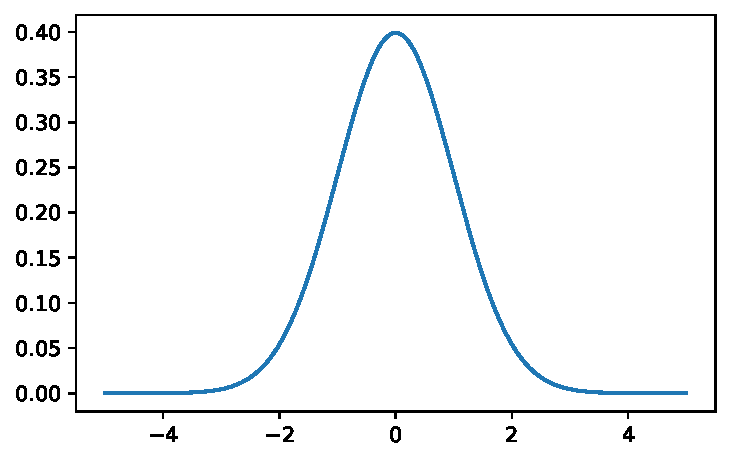
\includegraphics[keepaspectratio]{visualization_2/visualization_2_files/figure-pdf/cell-5-output-1.pdf}}

Alternatively, we can use \texttt{sns.histplot}. You can also get a very
similar result in a single call by requesting the KDE be added to the
histogram, with \texttt{kde=True} and some extra keywords:

\begin{Shaded}
\begin{Highlighting}[]
\NormalTok{plt.xlabel(}\StringTok{"Data"}\NormalTok{)}
\NormalTok{plt.xlim(}\OperatorTok{{-}}\DecValTok{3}\NormalTok{, }\DecValTok{10}\NormalTok{)}
\NormalTok{plt.ylim(}\DecValTok{0}\NormalTok{, }\FloatTok{0.5}\NormalTok{)}

\NormalTok{sns.histplot(data, bins}\OperatorTok{=}\DecValTok{2}\NormalTok{, kde}\OperatorTok{=}\VariableTok{True}\NormalTok{, stat}\OperatorTok{=}\StringTok{"density"}\NormalTok{, kde\_kws}\OperatorTok{=}\BuiltInTok{dict}\NormalTok{(cut}\OperatorTok{=}\DecValTok{3}\NormalTok{, bw\_method}\OperatorTok{=}\FloatTok{0.65}\NormalTok{))}\OperatorTok{;}
\end{Highlighting}
\end{Shaded}

\pandocbounded{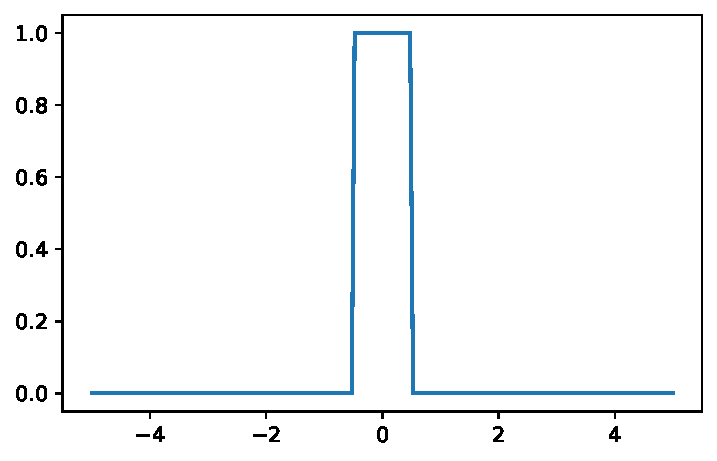
\includegraphics[keepaspectratio]{visualization_2/visualization_2_files/figure-pdf/cell-6-output-1.pdf}}

\subsubsection{Step 1: Place a Kernel at Each Data
Point}\label{step-1-place-a-kernel-at-each-data-point}

To begin generating a density curve, we need to choose a \textbf{kernel}
and \textbf{bandwidth value (\(\alpha\))}. What are these exactly?

A \textbf{kernel} is a density curve. It is the mathematical function
that attempts to capture the randomness of each data point in our
sampled data. To explain what this means, consider just \emph{one} of
the datapoints in our dataset: \(2.2\). We obtained this datapoint by
randomly sampling some information out in the real world (you can
imagine \(2.2\) as representing a single measurement taken in an
experiment, for example). If we were to sample a new datapoint, we may
obtain a slightly different value. It could be higher than \(2.2\); it
could also be lower than \(2.2\). We make the assumption that any future
sampled datapoints will likely be similar in value to the data we've
already drawn. This means that our \emph{kernel} -- our description of
the probability of randomly sampling any new value -- will be greatest
at the datapoint we've already drawn but still have non-zero probability
above and below it. The area under any kernel should integrate to 1,
representing the total probability of drawing a new datapoint.

A \textbf{bandwidth value}, usually denoted by \(\alpha\), represents
the width of the kernel. A large value of \(\alpha\) will result in a
wide, short kernel function, while a small value with result in a
narrow, tall kernel.

Below, we place a \textbf{Gaussian kernel}, plotted in orange, over the
datapoint \(2.2\). A Gaussian kernel is simply the normal distribution,
which you may have called a bell curve in Data 8.

\begin{Shaded}
\begin{Highlighting}[]
\KeywordTok{def}\NormalTok{ gaussian\_kernel(x, z, a):}
    \CommentTok{\# We\textquotesingle{}ll discuss where this mathematical formulation came from later}
    \ControlFlowTok{return}\NormalTok{ (}\DecValTok{1}\OperatorTok{/}\NormalTok{np.sqrt(}\DecValTok{2}\OperatorTok{*}\NormalTok{np.pi}\OperatorTok{*}\NormalTok{a}\OperatorTok{**}\DecValTok{2}\NormalTok{)) }\OperatorTok{*}\NormalTok{ np.exp((}\OperatorTok{{-}}\NormalTok{(x }\OperatorTok{{-}}\NormalTok{ z)}\OperatorTok{**}\DecValTok{2} \OperatorTok{/}\NormalTok{ (}\DecValTok{2} \OperatorTok{*}\NormalTok{ a}\OperatorTok{**}\DecValTok{2}\NormalTok{)))}

\CommentTok{\# Plot our datapoint}
\NormalTok{sns.rugplot([}\FloatTok{2.2}\NormalTok{], height}\OperatorTok{=}\FloatTok{0.3}\NormalTok{)}

\CommentTok{\# Plot the kernel}
\NormalTok{x }\OperatorTok{=}\NormalTok{ np.linspace(}\OperatorTok{{-}}\DecValTok{3}\NormalTok{, }\DecValTok{10}\NormalTok{, }\DecValTok{1000}\NormalTok{)}
\NormalTok{plt.plot(x, gaussian\_kernel(x, }\FloatTok{2.2}\NormalTok{, }\DecValTok{1}\NormalTok{))}

\NormalTok{plt.xlabel(}\StringTok{"Data"}\NormalTok{)}
\NormalTok{plt.ylabel(}\StringTok{"Density"}\NormalTok{)}
\NormalTok{plt.xlim(}\OperatorTok{{-}}\DecValTok{3}\NormalTok{, }\DecValTok{10}\NormalTok{)}
\NormalTok{plt.ylim(}\DecValTok{0}\NormalTok{, }\FloatTok{0.5}\NormalTok{)}\OperatorTok{;}
\end{Highlighting}
\end{Shaded}

\pandocbounded{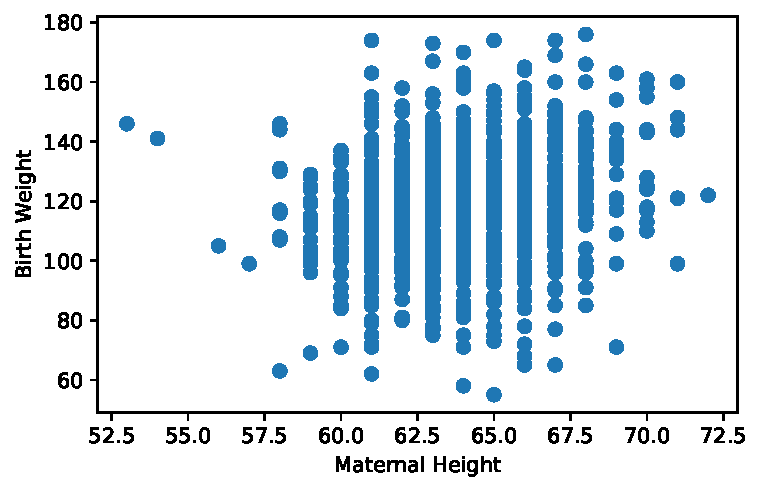
\includegraphics[keepaspectratio]{visualization_2/visualization_2_files/figure-pdf/cell-7-output-1.pdf}}

To begin creating our KDE, we place a kernel on \emph{each} datapoint in
our dataset. For our dataset of 5 points, we will have 5 kernels.

\begin{Shaded}
\begin{Highlighting}[]
\CommentTok{\# You will work with the functions below in Lab 4}
\KeywordTok{def}\NormalTok{ create\_kde(kernel, pts, a):}
    \CommentTok{\# Takes in a kernel, set of points, and alpha}
    \CommentTok{\# Returns the KDE as a function}
    \KeywordTok{def}\NormalTok{ f(x):}
\NormalTok{        output }\OperatorTok{=} \DecValTok{0}
        \ControlFlowTok{for}\NormalTok{ pt }\KeywordTok{in}\NormalTok{ pts:}
\NormalTok{            output }\OperatorTok{+=}\NormalTok{ kernel(x, pt, a)}
        \ControlFlowTok{return}\NormalTok{ output }\OperatorTok{/} \BuiltInTok{len}\NormalTok{(pts) }\CommentTok{\# Normalization factor}
    \ControlFlowTok{return}\NormalTok{ f}

\KeywordTok{def}\NormalTok{ plot\_kde(kernel, pts, a):}
    \CommentTok{\# Calls create\_kde and plots the corresponding KDE}
\NormalTok{    f }\OperatorTok{=}\NormalTok{ create\_kde(kernel, pts, a)}
\NormalTok{    x }\OperatorTok{=}\NormalTok{ np.linspace(}\BuiltInTok{min}\NormalTok{(pts) }\OperatorTok{{-}} \DecValTok{5}\NormalTok{, }\BuiltInTok{max}\NormalTok{(pts) }\OperatorTok{+} \DecValTok{5}\NormalTok{, }\DecValTok{1000}\NormalTok{)}
\NormalTok{    y }\OperatorTok{=}\NormalTok{ [f(xi) }\ControlFlowTok{for}\NormalTok{ xi }\KeywordTok{in}\NormalTok{ x]}
\NormalTok{    plt.plot(x, y)}\OperatorTok{;}
    
\KeywordTok{def}\NormalTok{ plot\_separate\_kernels(kernel, pts, a, norm}\OperatorTok{=}\VariableTok{False}\NormalTok{):}
    \CommentTok{\# Plots individual kernels, which are then summed to create the KDE}
\NormalTok{    x }\OperatorTok{=}\NormalTok{ np.linspace(}\BuiltInTok{min}\NormalTok{(pts) }\OperatorTok{{-}} \DecValTok{5}\NormalTok{, }\BuiltInTok{max}\NormalTok{(pts) }\OperatorTok{+} \DecValTok{5}\NormalTok{, }\DecValTok{1000}\NormalTok{)}
    \ControlFlowTok{for}\NormalTok{ pt }\KeywordTok{in}\NormalTok{ pts:}
\NormalTok{        y }\OperatorTok{=}\NormalTok{ kernel(x, pt, a)}
        \ControlFlowTok{if}\NormalTok{ norm:}
\NormalTok{            y }\OperatorTok{/=} \BuiltInTok{len}\NormalTok{(pts)}
\NormalTok{        plt.plot(x, y)}
    
\NormalTok{    plt.show()}\OperatorTok{;}
    
\NormalTok{plt.xlim(}\OperatorTok{{-}}\DecValTok{3}\NormalTok{, }\DecValTok{10}\NormalTok{)}
\NormalTok{plt.ylim(}\DecValTok{0}\NormalTok{, }\FloatTok{0.5}\NormalTok{)}
\NormalTok{plt.xlabel(}\StringTok{"Data"}\NormalTok{)}
\NormalTok{plt.ylabel(}\StringTok{"Density"}\NormalTok{)}

\NormalTok{plot\_separate\_kernels(gaussian\_kernel, data, a }\OperatorTok{=} \DecValTok{1}\NormalTok{)}
\end{Highlighting}
\end{Shaded}

\pandocbounded{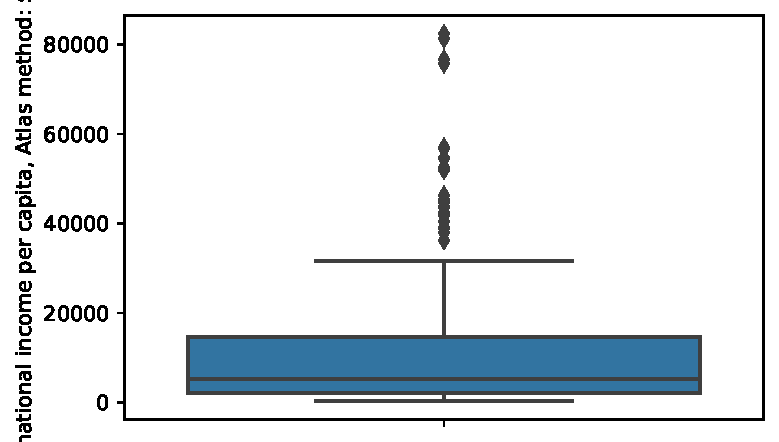
\includegraphics[keepaspectratio]{visualization_2/visualization_2_files/figure-pdf/cell-8-output-1.pdf}}

\subsubsection{Step 2: Normalize Kernels to Have a Total Area of
1}\label{step-2-normalize-kernels-to-have-a-total-area-of-1}

Above, we said that \emph{each} kernel has an area of 1. Earlier, we
also said that our goal is to construct a KDE curve using these kernels
with a \emph{total} area of 1. If we were to directly sum the kernels as
they are, we would produce a KDE curve with an integrated area of (5
kernels) \(\times\) (area of 1 each) = 5. To avoid this, we will
\textbf{normalize} each of our kernels. This involves multiplying each
kernel by \(\frac{1}{\#\:\text{datapoints}}\).

In the cell below, we multiply each of our 5 kernels by \(\frac{1}{5}\)
to apply normalization.

\begin{Shaded}
\begin{Highlighting}[]
\NormalTok{plt.xlim(}\OperatorTok{{-}}\DecValTok{3}\NormalTok{, }\DecValTok{10}\NormalTok{)}
\NormalTok{plt.ylim(}\DecValTok{0}\NormalTok{, }\FloatTok{0.5}\NormalTok{)}
\NormalTok{plt.xlabel(}\StringTok{"Data"}\NormalTok{)}
\NormalTok{plt.ylabel(}\StringTok{"Density"}\NormalTok{)}

\CommentTok{\# The \textasciigrave{}norm\textasciigrave{} argument specifies whether or not to normalize the kernels}
\NormalTok{plot\_separate\_kernels(gaussian\_kernel, data, a }\OperatorTok{=} \DecValTok{1}\NormalTok{, norm }\OperatorTok{=} \VariableTok{True}\NormalTok{)}
\end{Highlighting}
\end{Shaded}

\pandocbounded{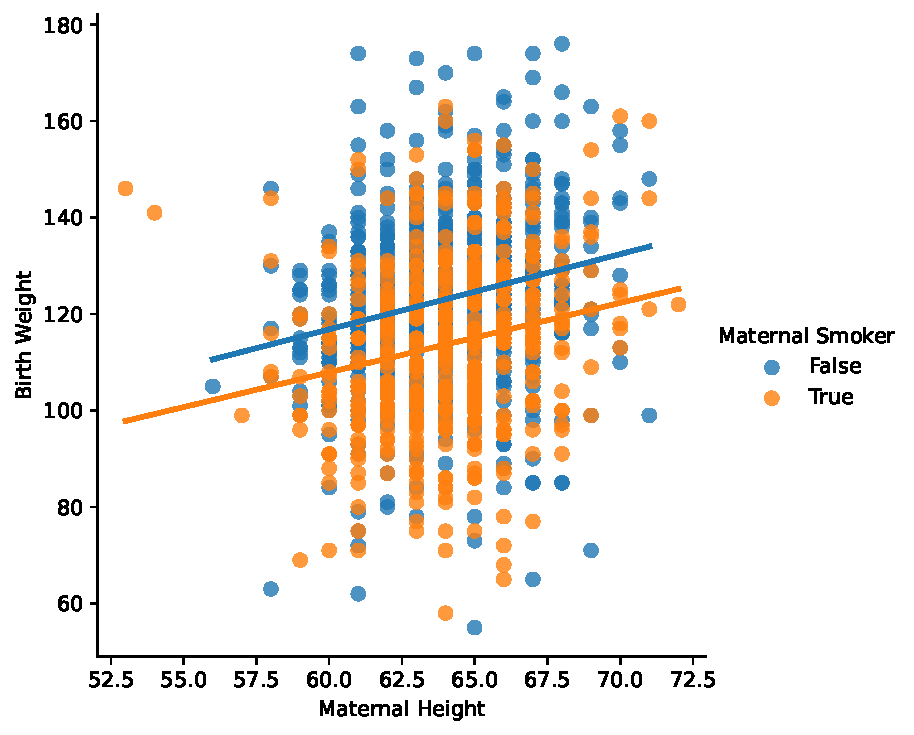
\includegraphics[keepaspectratio]{visualization_2/visualization_2_files/figure-pdf/cell-9-output-1.pdf}}

\subsubsection{Step 3: Sum the Normalized
Kernels}\label{step-3-sum-the-normalized-kernels}

Our KDE curve is the sum of the normalized kernels. Notice that the
final curve is identical to the plot generated by \texttt{sns.kdeplot}
we saw earlier!

\begin{Shaded}
\begin{Highlighting}[]
\NormalTok{plt.xlim(}\OperatorTok{{-}}\DecValTok{3}\NormalTok{, }\DecValTok{10}\NormalTok{)}
\NormalTok{plt.ylim(}\DecValTok{0}\NormalTok{, }\FloatTok{0.5}\NormalTok{)}
\NormalTok{plt.xlabel(}\StringTok{"Data"}\NormalTok{)}
\NormalTok{plt.ylabel(}\StringTok{"Density"}\NormalTok{)}

\NormalTok{plot\_kde(gaussian\_kernel, data, a}\OperatorTok{=}\DecValTok{1}\NormalTok{)}
\end{Highlighting}
\end{Shaded}

\pandocbounded{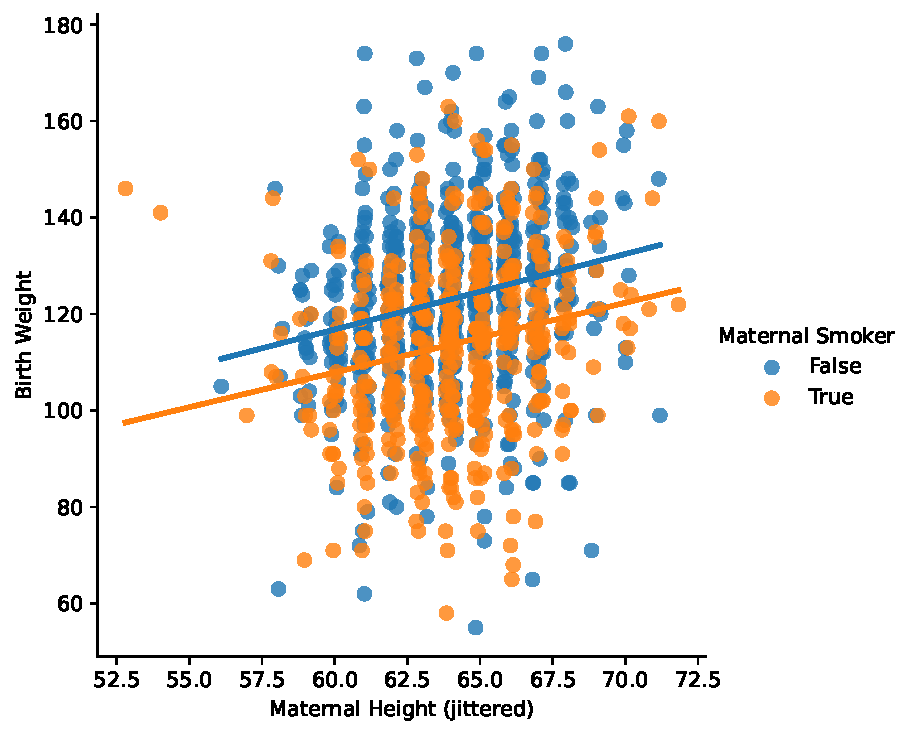
\includegraphics[keepaspectratio]{visualization_2/visualization_2_files/figure-pdf/cell-10-output-1.pdf}}

\subsection{Kernel Functions and
Bandwidths}\label{kernel-functions-and-bandwidths}

A general ``KDE formula'' function is given above.

\begin{enumerate}
\def\labelenumi{\arabic{enumi}.}
\tightlist
\item
  \(K_{\alpha}(x, x_i)\) is the kernel centered on the observation
  \texttt{i}.

  \begin{itemize}
  \tightlist
  \item
    Each kernel individually has area 1.
  \item
    x represents any number on the number line. It is the input to our
    function.
  \end{itemize}
\item
  \(n\) is the number of observed datapoints that we have.

  \begin{itemize}
  \tightlist
  \item
    We multiply by \(\frac{1}{n}\) so that the total area of the KDE is
    still 1.
  \end{itemize}
\item
  Each \(x_i \in \{x_1, x_2, \dots, x_n\}\) represents an observed
  datapoint.

  \begin{itemize}
  \tightlist
  \item
    These are what we use to create our KDE by summing multiple shifted
    kernels centered at these points.
  \end{itemize}
\end{enumerate}

\begin{itemize}
\tightlist
\item
  \(\alpha\) (alpha) is the bandwidth or smoothing parameter.
\end{itemize}

A \textbf{kernel} (for our purposes) is a valid density function. This
means it:

\begin{itemize}
\tightlist
\item
  Must be non-negative for all inputs.
\item
  Must integrate to 1.
\end{itemize}

\subsubsection{Gaussian Kernel}\label{gaussian-kernel}

The most common kernel is the \textbf{Gaussian kernel}. The Gaussian
kernel is equivalent to the Gaussian probability density function (the
Normal distribution), centered at the observed value with a standard
deviation of \(\alpha\) (this is known as the \textbf{bandwidth}
parameter).

\[K_a(x, x_i) = \frac{1}{\sqrt{2\pi\alpha^{2}}}e^{-\frac{(x-x_i)^{2}}{2\alpha^{2}}}\]

In this formula:

\begin{itemize}
\tightlist
\item
  \(x\) (no subscript) represents any value along the x-axis of our plot
\item
  \(x_i\) represents the \(i\) -th datapoint in our dataset. It is one
  of the values that we have actually collected in our data sampling
  process. In our example earlier, \(x_i=2.2\). Those of you who have
  taken a probability class may recognize \(x_i\) as the \textbf{mean}
  of the normal distribution.
\item
  Each kernel is \textbf{centered} on our observed values, so its
  distribution mean is \(x_i\).
\item
  \(\alpha\) is the bandwidth parameter, representing the width of our
  kernel. More formally, \(\alpha\) is the \textbf{standard deviation}
  of the Gaussian curve.

  \begin{itemize}
  \tightlist
  \item
    A large value of \(\alpha\) will produce a kernel that is wider and
    shorter -- this leads to a smoother KDE when the kernels are summed
    together.
  \item
    A small value of \(\alpha\) will produce a narrower, taller kernel,
    and, with it, a noisier KDE.
  \end{itemize}
\end{itemize}

The details of this (admittedly intimidating) formula are less important
than understanding its role in kernel density estimation -- this
equation gives us the shape of each kernel.

\begin{longtable}[]{@{}
  >{\raggedright\arraybackslash}p{(\linewidth - 2\tabcolsep) * \real{0.5000}}
  >{\raggedright\arraybackslash}p{(\linewidth - 2\tabcolsep) * \real{0.5000}}@{}}
\toprule\noalign{}
\begin{minipage}[b]{\linewidth}\raggedright
Gaussian Kernel, \(\alpha\) = 0.1
\end{minipage} & \begin{minipage}[b]{\linewidth}\raggedright
Gaussian Kernel, \(\alpha\) = 1
\end{minipage} \\
\midrule\noalign{}
\endhead
\bottomrule\noalign{}
\endlastfoot
& \\
\end{longtable}

\begin{longtable}[]{@{}
  >{\raggedright\arraybackslash}p{(\linewidth - 2\tabcolsep) * \real{0.5000}}
  >{\raggedright\arraybackslash}p{(\linewidth - 2\tabcolsep) * \real{0.5000}}@{}}
\toprule\noalign{}
\begin{minipage}[b]{\linewidth}\raggedright
Gaussian Kernel, \(\alpha\) = 2
\end{minipage} & \begin{minipage}[b]{\linewidth}\raggedright
Gaussian Kernel, \(\alpha\) = 5
\end{minipage} \\
\midrule\noalign{}
\endhead
\bottomrule\noalign{}
\endlastfoot
& \\
\end{longtable}

\subsubsection{Boxcar Kernel}\label{boxcar-kernel}

Another example of a kernel is the \textbf{Boxcar kernel}. The boxcar
kernel assigns a uniform density to points within a ``window'' of the
observation, and a density of 0 elsewhere. The equation below is a
boxcar kernel with the center at \(x_i\) and the bandwidth of
\(\alpha\).

\[K_a(x, x_i) = \begin{cases}
        \frac{1}{\alpha}, & |x - x_i| \le \frac{\alpha}{2}\\
        0, & \text{else }
    \end{cases}\]

The boxcar kernel is seldom used in practice -- we include it here to
demonstrate that a kernel function can take whatever form you would
like, provided it integrates to 1 and does not output negative values.

\begin{Shaded}
\begin{Highlighting}[]
\KeywordTok{def}\NormalTok{ boxcar\_kernel(alpha, x, z):}
    \ControlFlowTok{return}\NormalTok{ (((x}\OperatorTok{{-}}\NormalTok{z)}\OperatorTok{\textgreater{}={-}}\NormalTok{alpha}\OperatorTok{/}\DecValTok{2}\NormalTok{)}\OperatorTok{\&}\NormalTok{((x}\OperatorTok{{-}}\NormalTok{z)}\OperatorTok{\textless{}=}\NormalTok{alpha}\OperatorTok{/}\DecValTok{2}\NormalTok{))}\OperatorTok{/}\NormalTok{alpha}

\NormalTok{xs }\OperatorTok{=}\NormalTok{ np.linspace(}\OperatorTok{{-}}\DecValTok{5}\NormalTok{, }\DecValTok{5}\NormalTok{, }\DecValTok{200}\NormalTok{)}
\NormalTok{alpha}\OperatorTok{=}\DecValTok{1}
\NormalTok{kde\_curve }\OperatorTok{=}\NormalTok{ [boxcar\_kernel(alpha, x, }\DecValTok{0}\NormalTok{) }\ControlFlowTok{for}\NormalTok{ x }\KeywordTok{in}\NormalTok{ xs]}
\NormalTok{plt.plot(xs, kde\_curve)}\OperatorTok{;}
\end{Highlighting}
\end{Shaded}

\begin{figure}[H]

{\centering \pandocbounded{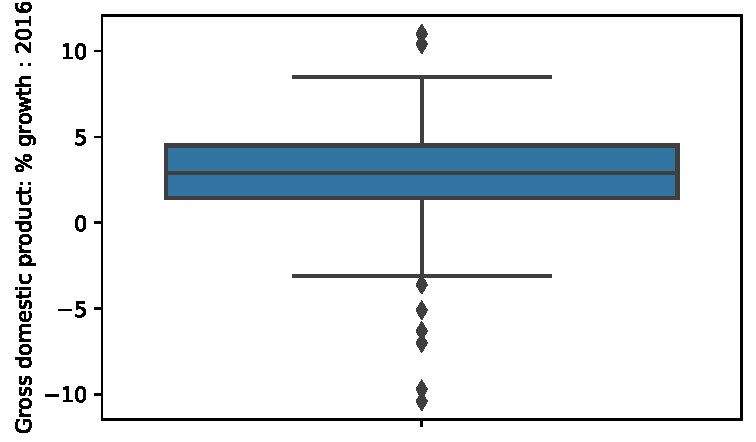
\includegraphics[keepaspectratio]{visualization_2/visualization_2_files/figure-pdf/cell-11-output-1.pdf}}

}

\caption{The Boxcar kernel centered at 0 with bandwidth \(\alpha\) = 1.}

\end{figure}%

The diagram on the right is how the density curve for our 5 point
dataset would have looked had we used the Boxcar kernel with bandwidth
\(\alpha\) = 1.

\begin{longtable}[]{@{}
  >{\raggedright\arraybackslash}p{(\linewidth - 2\tabcolsep) * \real{0.5000}}
  >{\raggedright\arraybackslash}p{(\linewidth - 2\tabcolsep) * \real{0.5000}}@{}}
\toprule\noalign{}
\begin{minipage}[b]{\linewidth}\raggedright
KDE
\end{minipage} & \begin{minipage}[b]{\linewidth}\raggedright
Boxcar
\end{minipage} \\
\midrule\noalign{}
\endhead
\bottomrule\noalign{}
\endlastfoot
& \\
\end{longtable}

\section{\texorpdfstring{Diving Deeper into
\texttt{displot}}{Diving Deeper into displot}}\label{diving-deeper-into-displot}

As we saw earlier, we can use \texttt{seaborn}'s \texttt{displot}
function to plot various distributions. In particular, \texttt{displot}
allows you to specify the \texttt{kind} of plot and is a wrapper for
\texttt{histplot}, \texttt{kdeplot}, and \texttt{ecdfplot}.

Below, we can see a couple of examples of how \texttt{sns.displot} can
be used to plot various distributions.

First, we can plot a histogram by setting \texttt{kind} to
\texttt{"hist"}. Note that here we've specified
\texttt{stat\ =\ density} to normalize the histogram such that the area
under the histogram is equal to 1.

\begin{Shaded}
\begin{Highlighting}[]
\NormalTok{sns.displot(data}\OperatorTok{=}\NormalTok{wb, }
\NormalTok{            x}\OperatorTok{=}\StringTok{"gni"}\NormalTok{, }
\NormalTok{            kind}\OperatorTok{=}\StringTok{"hist"}\NormalTok{, }
\NormalTok{            stat}\OperatorTok{=}\StringTok{"density"}\NormalTok{) }\CommentTok{\# default: stat=count and density integrates to 1}
\NormalTok{plt.title(}\StringTok{"Distribution of gross national income per capita"}\NormalTok{)}\OperatorTok{;}
\end{Highlighting}
\end{Shaded}

\pandocbounded{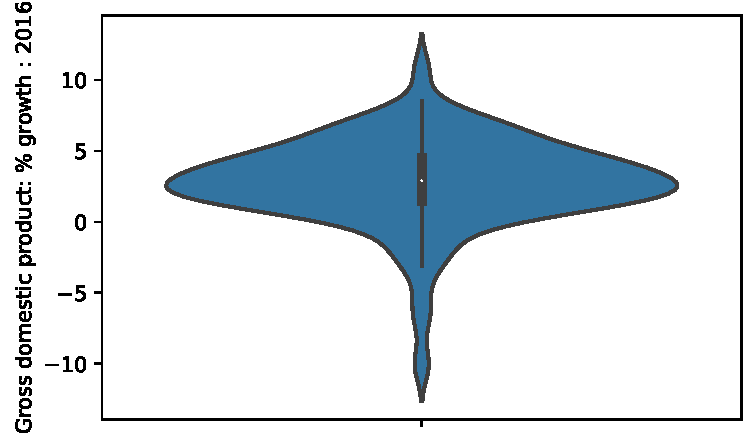
\includegraphics[keepaspectratio]{visualization_2/visualization_2_files/figure-pdf/cell-12-output-1.pdf}}

Now, what if we want to generate a KDE plot? We can set \texttt{kind} =
to \texttt{"kde"}!

\begin{Shaded}
\begin{Highlighting}[]
\NormalTok{sns.displot(data}\OperatorTok{=}\NormalTok{wb, }
\NormalTok{            x}\OperatorTok{=}\StringTok{"gni"}\NormalTok{, }
\NormalTok{            kind}\OperatorTok{=}\StringTok{\textquotesingle{}kde\textquotesingle{}}\NormalTok{)}
\NormalTok{plt.title(}\StringTok{"Distribution of gross national income per capita"}\NormalTok{)}\OperatorTok{;}
\end{Highlighting}
\end{Shaded}

\pandocbounded{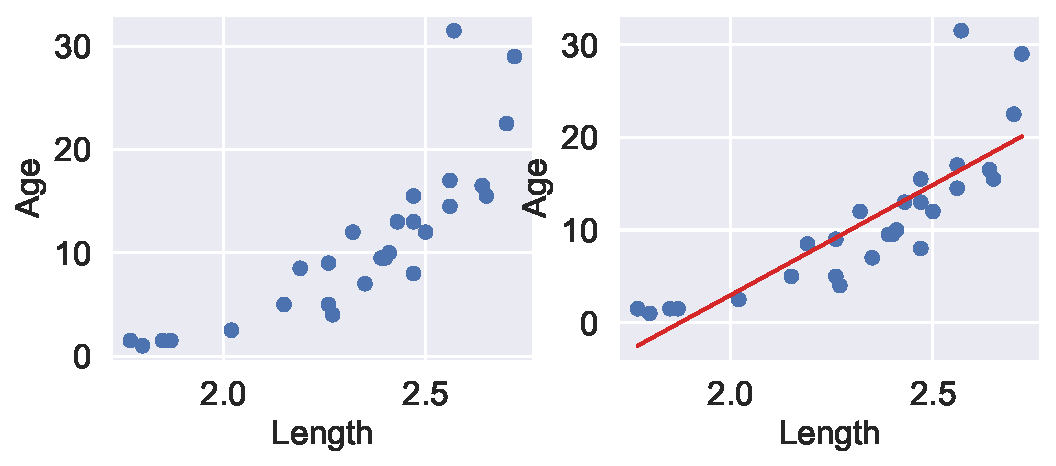
\includegraphics[keepaspectratio]{visualization_2/visualization_2_files/figure-pdf/cell-13-output-1.pdf}}

And finally, if we want to generate an Empirical Cumulative Distribution
Function (ECDF), we can specify \texttt{kind\ =\ "ecdf"}.

\begin{Shaded}
\begin{Highlighting}[]
\NormalTok{sns.displot(data}\OperatorTok{=}\NormalTok{wb, }
\NormalTok{            x}\OperatorTok{=}\StringTok{"gni"}\NormalTok{, }
\NormalTok{            kind}\OperatorTok{=}\StringTok{\textquotesingle{}ecdf\textquotesingle{}}\NormalTok{)}
\NormalTok{plt.title(}\StringTok{"Cumulative Distribution of gross national income per capita"}\NormalTok{)}\OperatorTok{;}
\end{Highlighting}
\end{Shaded}

\pandocbounded{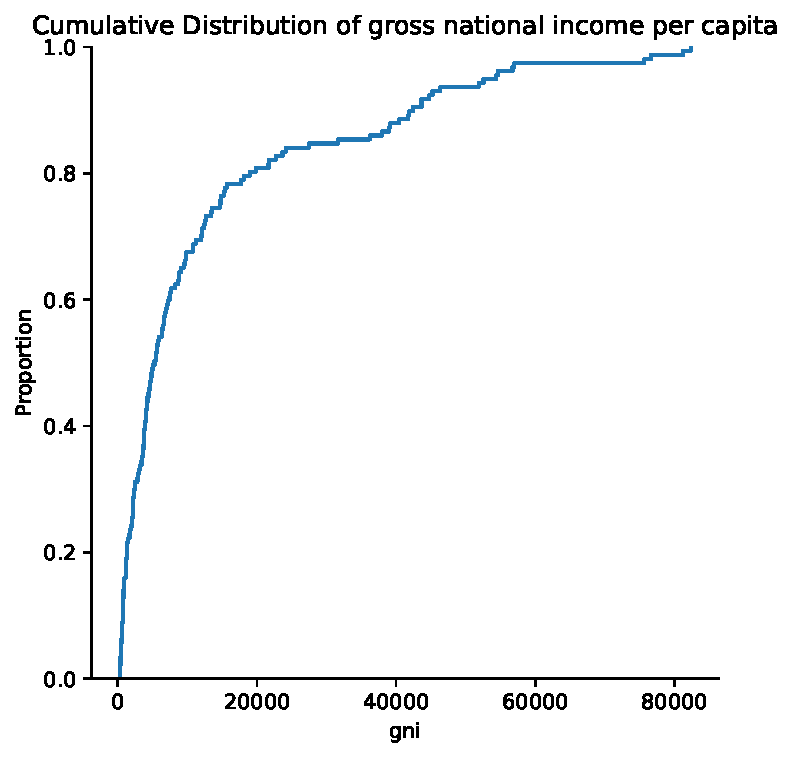
\includegraphics[keepaspectratio]{visualization_2/visualization_2_files/figure-pdf/cell-14-output-1.pdf}}

\section{Relationships Between Quantitative
Variables}\label{relationships-between-quantitative-variables}

Up until now, we've discussed how to visualize single-variable
distributions. Going beyond this, we want to understand the relationship
between pairs of numerical variables.

\subsubsection{Scatter Plots}\label{scatter-plots}

\textbf{Scatter plots} are one of the most useful tools in representing
the relationship between \textbf{pairs} of quantitative variables. They
are particularly important in gauging the strength, or correlation, of
the relationship between variables. Knowledge of these relationships can
then motivate decisions in our modeling process.

In \texttt{matplotlib}, we use the function \texttt{plt.scatter} to
generate a scatter plot. Notice that, unlike our examples of plotting
single-variable distributions, now we specify sequences of values to be
plotted along the x-axis \emph{and} the y-axis.

\begin{Shaded}
\begin{Highlighting}[]
\NormalTok{plt.scatter(wb[}\StringTok{"per capita: }\SpecialCharTok{\% g}\StringTok{rowth: 2016"}\NormalTok{], }\OperatorTok{\textbackslash{}}
\NormalTok{            wb[}\StringTok{\textquotesingle{}Adult literacy rate: Female: \% ages 15 and older: 2005{-}14\textquotesingle{}}\NormalTok{])}

\NormalTok{plt.xlabel(}\StringTok{"}\SpecialCharTok{\% g}\StringTok{rowth per capita"}\NormalTok{)}
\NormalTok{plt.ylabel(}\StringTok{"Female adult literacy rate"}\NormalTok{)}
\NormalTok{plt.title(}\StringTok{"Female adult literacy against }\SpecialCharTok{\% g}\StringTok{rowth"}\NormalTok{)}\OperatorTok{;}
\end{Highlighting}
\end{Shaded}

\pandocbounded{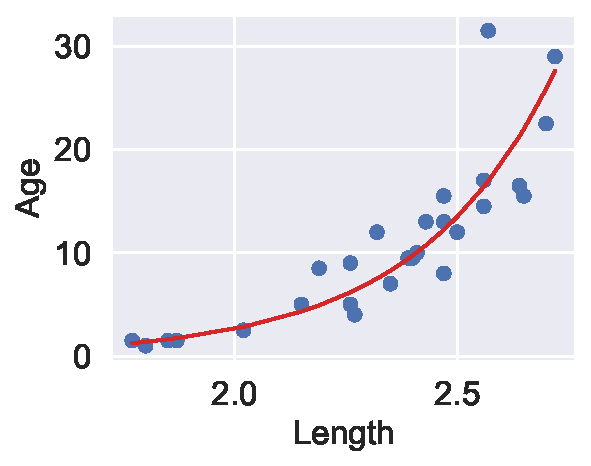
\includegraphics[keepaspectratio]{visualization_2/visualization_2_files/figure-pdf/cell-15-output-1.pdf}}

In \texttt{seaborn}, we call the function \texttt{sns.scatterplot}. We
use the \texttt{x} and \texttt{y} parameters to indicate the values to
be plotted along the x and y axes, respectively. By using the
\texttt{hue} parameter, we can specify a third variable to be used for
coloring each scatter point.

\begin{Shaded}
\begin{Highlighting}[]
\NormalTok{sns.scatterplot(data }\OperatorTok{=}\NormalTok{ wb, x }\OperatorTok{=} \StringTok{"per capita: }\SpecialCharTok{\% g}\StringTok{rowth: 2016"}\NormalTok{, }\OperatorTok{\textbackslash{}}
\NormalTok{               y }\OperatorTok{=} \StringTok{"Adult literacy rate: Female: \% ages 15 and older: 2005{-}14"}\NormalTok{, }
\NormalTok{               hue }\OperatorTok{=} \StringTok{"Continent"}\NormalTok{)}

\NormalTok{plt.title(}\StringTok{"Female adult literacy against }\SpecialCharTok{\% g}\StringTok{rowth"}\NormalTok{)}\OperatorTok{;}
\end{Highlighting}
\end{Shaded}

\pandocbounded{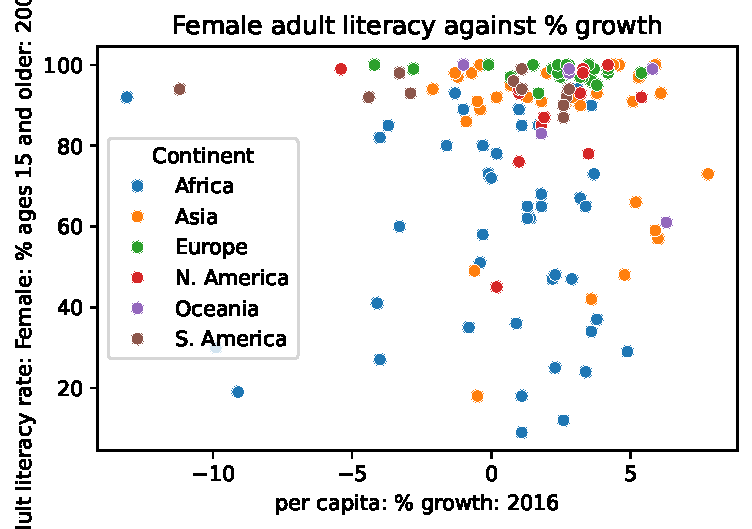
\includegraphics[keepaspectratio]{visualization_2/visualization_2_files/figure-pdf/cell-16-output-1.pdf}}

\paragraph{Overplotting}\label{overplotting}

Although the plots above communicate the general relationship between
the two plotted variables, they both suffer a major limitation --
\textbf{overplotting}. Overplotting occurs when scatter points with
similar values are stacked on top of one another, making it difficult to
see the number of scatter points actually plotted in the visualization.
Notice how in the upper righthand region of the plots, we cannot easily
tell just how many points have been plotted. This makes our
visualizations difficult to interpret.

We have a few methods to help reduce overplotting:

\begin{itemize}
\tightlist
\item
  Decreasing the size of the scatter point markers can improve
  readability. We do this by setting a new value to the size parameter,
  \texttt{s}, of \texttt{plt.scatter} or \texttt{sns.scatterplot}.
\item
  \textbf{Jittering} is the process of adding a small amount of random
  noise to all x and y values to slightly shift the position of each
  datapoint. By randomly shifting all the data by some small distance,
  we can discern individual points more clearly without modifying the
  major trends of the original dataset.
\end{itemize}

In the cell below, we first jitter the data using
\texttt{np.random.uniform}, then re-plot it with smaller markers. The
resulting plot is much easier to interpret.

\begin{Shaded}
\begin{Highlighting}[]
\CommentTok{\# Setting a seed ensures that we produce the same plot each time}
\CommentTok{\# This means that the course notes will not change each time you access them}
\NormalTok{np.random.seed(}\DecValTok{150}\NormalTok{)}

\CommentTok{\# This call to np.random.uniform generates random numbers between {-}1 and 1}
\CommentTok{\# We add these random numbers to the original x data to jitter it slightly}
\NormalTok{x\_noise }\OperatorTok{=}\NormalTok{ np.random.uniform(}\OperatorTok{{-}}\DecValTok{1}\NormalTok{, }\DecValTok{1}\NormalTok{, }\BuiltInTok{len}\NormalTok{(wb))}
\NormalTok{jittered\_x }\OperatorTok{=}\NormalTok{ wb[}\StringTok{"per capita: }\SpecialCharTok{\% g}\StringTok{rowth: 2016"}\NormalTok{] }\OperatorTok{+}\NormalTok{ x\_noise}

\CommentTok{\# Repeat for y data}
\NormalTok{y\_noise }\OperatorTok{=}\NormalTok{ np.random.uniform(}\OperatorTok{{-}}\DecValTok{5}\NormalTok{, }\DecValTok{5}\NormalTok{, }\BuiltInTok{len}\NormalTok{(wb))}
\NormalTok{jittered\_y }\OperatorTok{=}\NormalTok{ wb[}\StringTok{"Adult literacy rate: Female: \% ages 15 and older: 2005{-}14"}\NormalTok{] }\OperatorTok{+}\NormalTok{ y\_noise}

\CommentTok{\# Setting the size parameter \textasciigrave{}s\textasciigrave{} changes the size of each point}
\NormalTok{plt.scatter(jittered\_x, jittered\_y, s}\OperatorTok{=}\DecValTok{15}\NormalTok{)}

\NormalTok{plt.xlabel(}\StringTok{"}\SpecialCharTok{\% g}\StringTok{rowth per capita (jittered)"}\NormalTok{)}
\NormalTok{plt.ylabel(}\StringTok{"Female adult literacy rate (jittered)"}\NormalTok{)}
\NormalTok{plt.title(}\StringTok{"Female adult literacy against }\SpecialCharTok{\% g}\StringTok{rowth"}\NormalTok{)}\OperatorTok{;}
\end{Highlighting}
\end{Shaded}

\pandocbounded{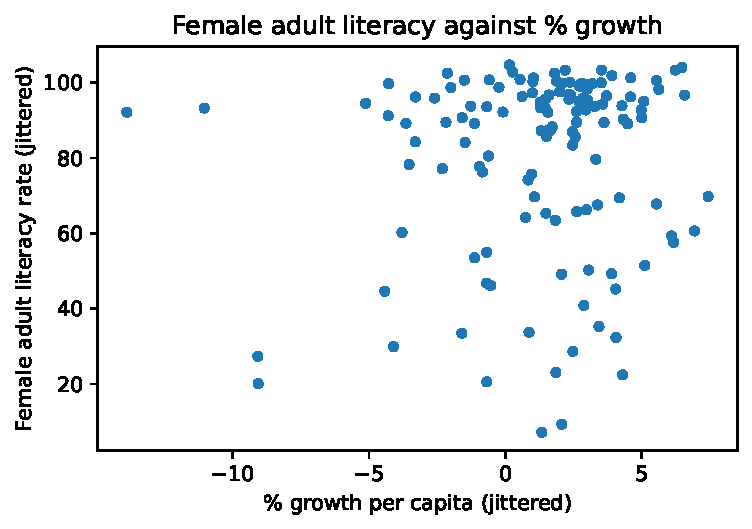
\includegraphics[keepaspectratio]{visualization_2/visualization_2_files/figure-pdf/cell-17-output-1.pdf}}

\subsubsection{\texorpdfstring{\texttt{lmplot} and
\texttt{jointplot}}{lmplot and jointplot}}\label{lmplot-and-jointplot}

\texttt{seaborn} also includes several built-in functions for creating
more sophisticated scatter plots. Two of the most commonly used examples
are \texttt{sns.lmplot} and \texttt{sns.jointplot}.

\texttt{sns.lmplot} plots both a scatter plot \emph{and} a linear
regression line, all in one function call. We'll discuss linear
regression in a few lectures.

\begin{Shaded}
\begin{Highlighting}[]
\NormalTok{sns.lmplot(data }\OperatorTok{=}\NormalTok{ wb, x }\OperatorTok{=} \StringTok{"per capita: }\SpecialCharTok{\% g}\StringTok{rowth: 2016"}\NormalTok{, }\OperatorTok{\textbackslash{}}
\NormalTok{           y }\OperatorTok{=} \StringTok{"Adult literacy rate: Female: \% ages 15 and older: 2005{-}14"}\NormalTok{)}

\NormalTok{plt.title(}\StringTok{"Female adult literacy against }\SpecialCharTok{\% g}\StringTok{rowth"}\NormalTok{)}\OperatorTok{;}
\end{Highlighting}
\end{Shaded}

\pandocbounded{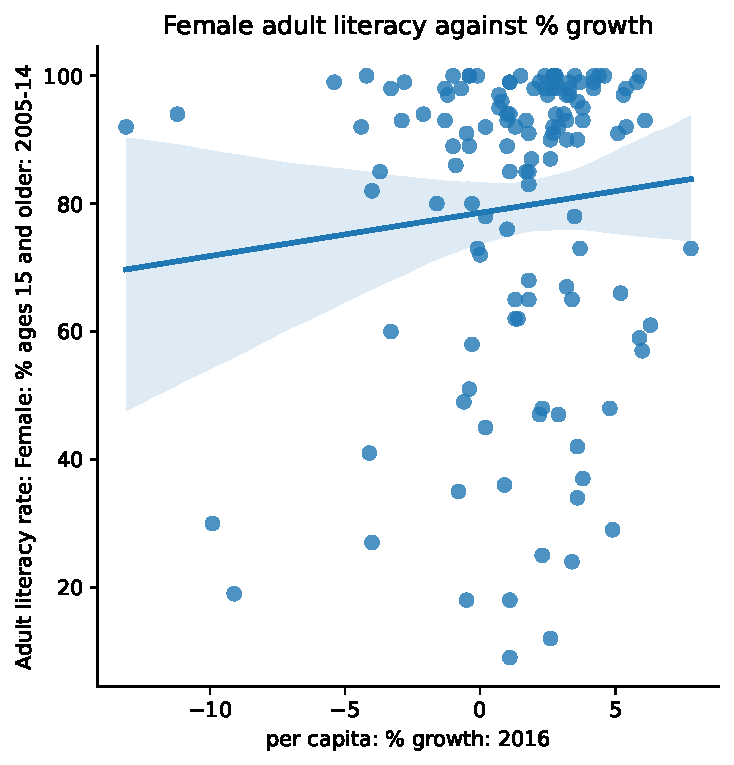
\includegraphics[keepaspectratio]{visualization_2/visualization_2_files/figure-pdf/cell-18-output-1.pdf}}

\texttt{sns.jointplot} creates a visualization with three components: a
scatter plot, a histogram of the distribution of x values, and a
histogram of the distribution of y values.

\begin{Shaded}
\begin{Highlighting}[]
\NormalTok{sns.jointplot(data }\OperatorTok{=}\NormalTok{ wb, x }\OperatorTok{=} \StringTok{"per capita: }\SpecialCharTok{\% g}\StringTok{rowth: 2016"}\NormalTok{, }\OperatorTok{\textbackslash{}}
\NormalTok{           y }\OperatorTok{=} \StringTok{"Adult literacy rate: Female: \% ages 15 and older: 2005{-}14"}\NormalTok{)}

\CommentTok{\# plt.suptitle allows us to shift the title up so it does not overlap with the histogram}
\NormalTok{plt.suptitle(}\StringTok{"Female adult literacy against }\SpecialCharTok{\% g}\StringTok{rowth"}\NormalTok{)}
\NormalTok{plt.subplots\_adjust(top}\OperatorTok{=}\FloatTok{0.9}\NormalTok{)}\OperatorTok{;}
\end{Highlighting}
\end{Shaded}

\pandocbounded{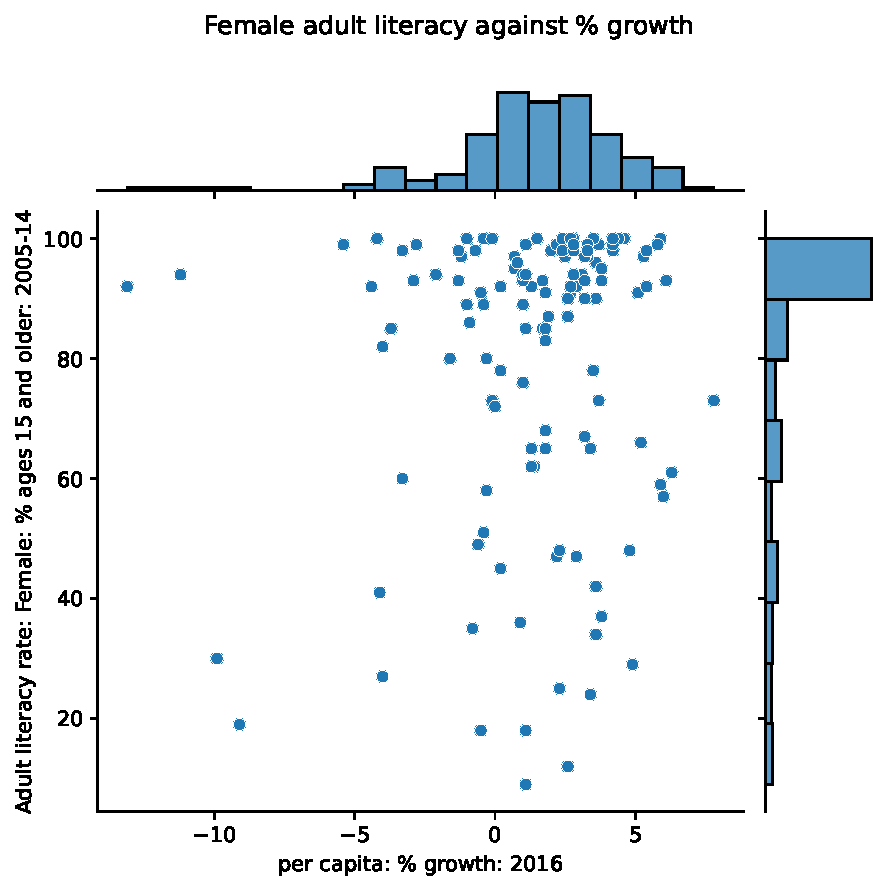
\includegraphics[keepaspectratio]{visualization_2/visualization_2_files/figure-pdf/cell-19-output-1.pdf}}

\subsubsection{Hex plots}\label{hex-plots}

For datasets with a very large number of datapoints, jittering is
unlikely to fully resolve the issue of overplotting. In these cases, we
can attempt to visualize our data by its \emph{density}, rather than
displaying each individual datapoint.

\textbf{Hex plots} can be thought of as two-dimensional histograms that
show the joint distribution between two variables. This is particularly
useful when working with very dense data. In a hex plot, the x-y plane
is binned into hexagons. Hexagons that are darker in color indicate a
greater density of data -- that is, there are more data points that lie
in the region enclosed by the hexagon.

We can generate a hex plot using \texttt{sns.jointplot} modified with
the \texttt{kind} parameter.

\begin{Shaded}
\begin{Highlighting}[]
\NormalTok{sns.jointplot(data }\OperatorTok{=}\NormalTok{ wb, x }\OperatorTok{=} \StringTok{"per capita: }\SpecialCharTok{\% g}\StringTok{rowth: 2016"}\NormalTok{, }\OperatorTok{\textbackslash{}}
\NormalTok{              y }\OperatorTok{=} \StringTok{"Adult literacy rate: Female: \% ages 15 and older: 2005{-}14"}\NormalTok{, }\OperatorTok{\textbackslash{}}
\NormalTok{              kind }\OperatorTok{=} \StringTok{"hex"}\NormalTok{)}

\CommentTok{\# plt.suptitle allows us to shift the title up so it does not overlap with the histogram}
\NormalTok{plt.suptitle(}\StringTok{"Female adult literacy against }\SpecialCharTok{\% g}\StringTok{rowth"}\NormalTok{)}
\NormalTok{plt.subplots\_adjust(top}\OperatorTok{=}\FloatTok{0.9}\NormalTok{)}\OperatorTok{;}
\end{Highlighting}
\end{Shaded}

\pandocbounded{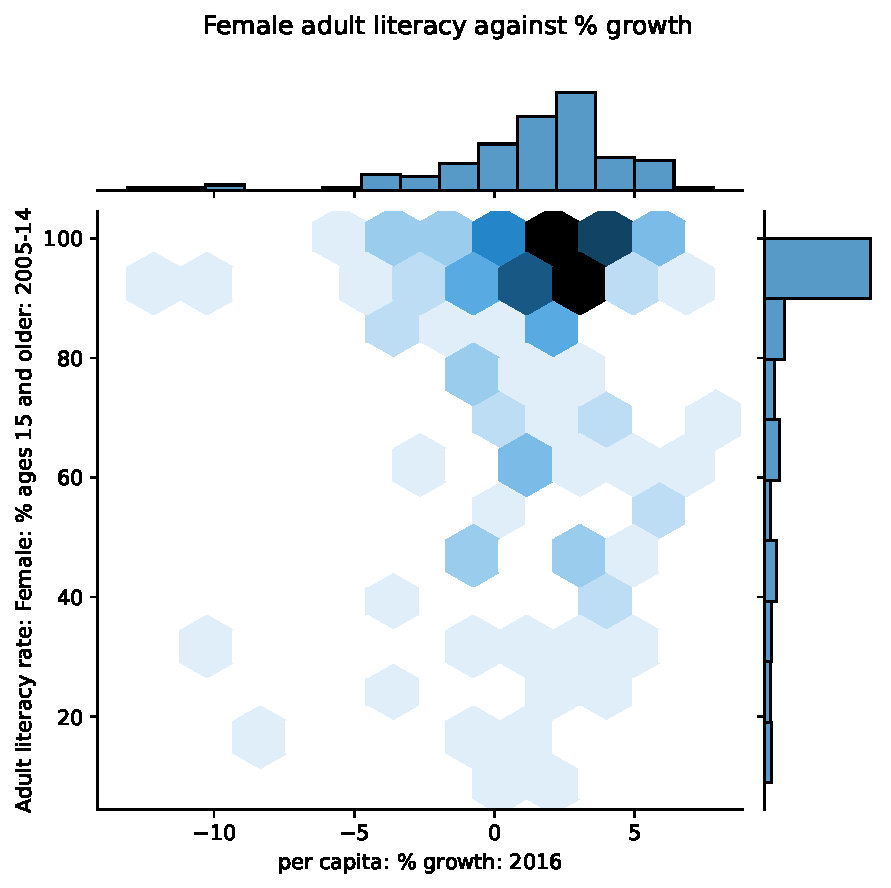
\includegraphics[keepaspectratio]{visualization_2/visualization_2_files/figure-pdf/cell-20-output-1.pdf}}

\subsubsection{Contour Plots}\label{contour-plots}

\textbf{Contour plots} are an alternative way of plotting the joint
distribution of two variables. You can think of them as the
2-dimensional versions of KDE plots. A contour plot can be interpreted
in a similar way to a
\href{https://gisgeography.com/contour-lines-topographic-map/}{topographic
map}. Each contour line represents an area that has the same
\emph{density} of datapoints throughout the region. Contours marked with
darker colors contain more datapoints (a higher density) in that region.

\texttt{sns.kdeplot} will generate a contour plot if we specify both x
and y data.

\begin{Shaded}
\begin{Highlighting}[]
\NormalTok{sns.kdeplot(data }\OperatorTok{=}\NormalTok{ wb, x }\OperatorTok{=} \StringTok{"per capita: }\SpecialCharTok{\% g}\StringTok{rowth: 2016"}\NormalTok{, }\OperatorTok{\textbackslash{}}
\NormalTok{            y }\OperatorTok{=} \StringTok{"Adult literacy rate: Female: \% ages 15 and older: 2005{-}14"}\NormalTok{, }\OperatorTok{\textbackslash{}}
\NormalTok{            fill }\OperatorTok{=} \VariableTok{True}\NormalTok{)}

\NormalTok{plt.title(}\StringTok{"Female adult literacy against }\SpecialCharTok{\% g}\StringTok{rowth"}\NormalTok{)}\OperatorTok{;}
\end{Highlighting}
\end{Shaded}

\pandocbounded{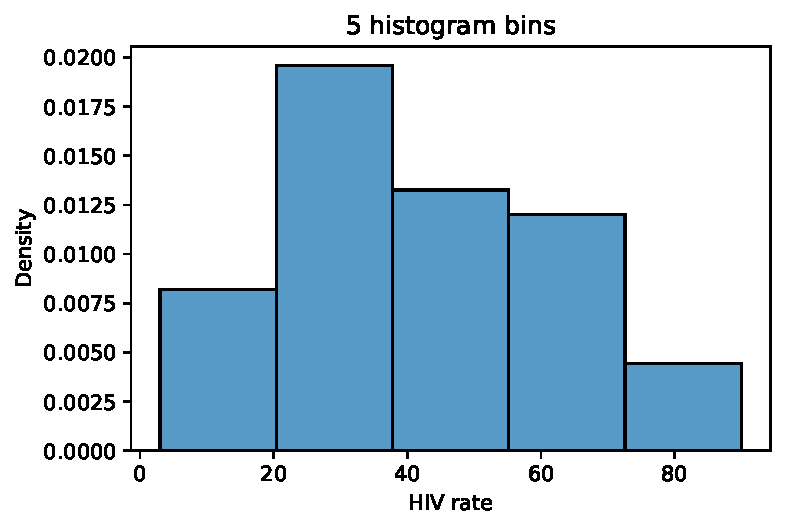
\includegraphics[keepaspectratio]{visualization_2/visualization_2_files/figure-pdf/cell-21-output-1.pdf}}

\section{Transformations}\label{transformations}

We have now covered visualizations in great depth, looking into various
forms of visualizations, plotting libraries, and high-level theory.

Much of this was done to uncover insights in data, which will prove
necessary when we begin building models of data later in the course. A
strong graphical correlation between two variables hints at an
underlying relationship that we may want to study in greater detail.
However, relying on visual relationships alone is limiting - not all
plots show association. The presence of outliers and other statistical
anomalies makes it hard to interpret data.

\textbf{Transformations} are the process of manipulating data to find
significant relationships between variables. These are often found by
applying mathematical functions to variables that ``transform'' their
range of possible values and highlight some previously hidden
associations between data.

To see why we may want to transform data, consider the following plot of
adult literacy rates against gross national income.

\begin{Shaded}
\begin{Highlighting}[]
\CommentTok{\# Some data cleaning to help with the next example}
\NormalTok{df }\OperatorTok{=}\NormalTok{ pd.DataFrame(index}\OperatorTok{=}\NormalTok{wb.index)}
\NormalTok{df[}\StringTok{\textquotesingle{}lit\textquotesingle{}}\NormalTok{] }\OperatorTok{=}\NormalTok{ wb[}\StringTok{\textquotesingle{}Adult literacy rate: Female: \% ages 15 and older: 2005{-}14\textquotesingle{}}\NormalTok{] }\OperatorTok{\textbackslash{}}
            \OperatorTok{+}\NormalTok{ wb[}\StringTok{"Adult literacy rate: Male: \% ages 15 and older: 2005{-}14"}\NormalTok{]}
\NormalTok{df[}\StringTok{\textquotesingle{}inc\textquotesingle{}}\NormalTok{] }\OperatorTok{=}\NormalTok{ wb[}\StringTok{\textquotesingle{}gni\textquotesingle{}}\NormalTok{]}
\NormalTok{df.dropna(inplace}\OperatorTok{=}\VariableTok{True}\NormalTok{)}

\NormalTok{plt.scatter(df[}\StringTok{"inc"}\NormalTok{], df[}\StringTok{"lit"}\NormalTok{])}
\NormalTok{plt.xlabel(}\StringTok{"Gross national income per capita"}\NormalTok{)}
\NormalTok{plt.ylabel(}\StringTok{"Adult literacy rate"}\NormalTok{)}
\NormalTok{plt.title(}\StringTok{"Adult literacy rate against GNI per capita"}\NormalTok{)}\OperatorTok{;}
\end{Highlighting}
\end{Shaded}

\pandocbounded{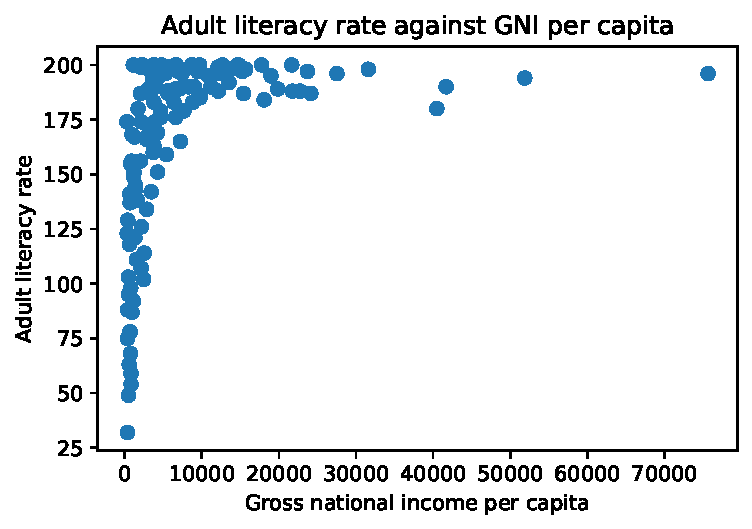
\includegraphics[keepaspectratio]{visualization_2/visualization_2_files/figure-pdf/cell-22-output-1.pdf}}

This plot is difficult to interpret for two reasons:

\begin{itemize}
\tightlist
\item
  The data shown in the visualization appears almost ``smushed'' -- it
  is heavily concentrated in the upper lefthand region of the plot. Even
  if we jittered the dataset, we likely would not be able to fully
  assess all datapoints in that area.
\item
  It is hard to generalize a clear relationship between the two plotted
  variables. While adult literacy rate appears to share some positive
  relationship with gross national income, we are not able to describe
  the specifics of this trend in much detail.
\end{itemize}

A transformation would allow us to visualize this data more clearly,
which, in turn, would enable us to describe the underlying relationship
between our variables of interest.

We will most commonly apply a transformation to \textbf{linearize a
relationship} between variables. If we find a transformation to make a
scatter plot of two variables linear, we can ``backtrack'' to find the
exact relationship between the variables. This helps us in two major
ways. Firstly, linear relationships are particularly simple to interpret
-- we have an intuitive sense of what the slope and intercept of a
linear trend represent, and how they can help us understand the
relationship between two variables. Secondly, linear relationships are
the backbone of linear models. We will begin exploring linear modeling
in great detail next week. As we'll soon see, linear models become much
more effective when we are working with linearized data.

In the remainder of this note, we will discuss how to linearize a
dataset to produce the result below. Notice that the resulting plot
displays a rough linear relationship between the values plotted on the x
and y axes.

\subsection{Linearization and Applying
Transformations}\label{linearization-and-applying-transformations}

To linearize a relationship, begin by asking yourself: what makes the
data non-linear? It is helpful to repeat this question for each variable
in your visualization.

Let's start by considering the gross national income variable in our
plot above. Looking at the y values in the scatter plot, we can see that
many large y values are all clumped together, compressing the vertical
axis. The scale of the horizontal axis is also being distorted by the
few large outlying x values on the right.

If we decreased the size of these outliers relative to the bulk of the
data, we could reduce the distortion of the horizontal axis. How can we
do this? We need a transformation that will:

\begin{itemize}
\tightlist
\item
  Decrease the magnitude of large x values by a significant amount.
\item
  Not drastically change the magnitude of small x values.
\end{itemize}

One function that produces this result is the \textbf{log
transformation}. When we take the logarithm of a large number, the
original number will decrease in magnitude dramatically. Conversely,
when we take the logarithm of a small number, the original number does
not change its value by as significant of an amount (to illustrate this,
consider the difference between \(\log{(100)} = 4.61\) and
\(\log{(10)} = 2.3\)).

In Data 100 (and most upper-division STEM classes), \(\log\) is used to
refer to the natural logarithm with base \(e\).

\begin{Shaded}
\begin{Highlighting}[]
\CommentTok{\# np.log takes the logarithm of an array or Series}
\NormalTok{plt.scatter(np.log(df[}\StringTok{"inc"}\NormalTok{]), df[}\StringTok{"lit"}\NormalTok{])}

\NormalTok{plt.xlabel(}\StringTok{"Log(gross national income per capita)"}\NormalTok{)}
\NormalTok{plt.ylabel(}\StringTok{"Adult literacy rate"}\NormalTok{)}
\NormalTok{plt.title(}\StringTok{"Adult literacy rate against Log(GNI per capita)"}\NormalTok{)}\OperatorTok{;}
\end{Highlighting}
\end{Shaded}

\pandocbounded{\includegraphics[keepaspectratio]{visualization_2/visualization_2_files/figure-pdf/cell-23-output-1.pdf}}

After taking the logarithm of our x values, our plot appears much more
balanced in its horizontal scale. We no longer have many datapoints
clumped on one end and a few outliers out at extreme values.

Let's repeat this reasoning for the y values. Considering only the
vertical axis of the plot, notice how there are many datapoints
concentrated at large y values. Only a few datapoints lie at smaller
values of y.

If we were to ``spread out'' these large values of y more, we would no
longer see the dense concentration in one region of the y-axis. We need
a transformation that will:

\begin{itemize}
\tightlist
\item
  Increase the magnitude of large values of y so these datapoints are
  distributed more broadly on the vertical scale,
\item
  Not substantially alter the scaling of small values of y (we do not
  want to drastically modify the lower end of the y axis, which is
  already distributed evenly on the vertical scale).
\end{itemize}

In this case, it is helpful to apply a \textbf{power transformation} --
that is, raise our y values to a power. Let's try raising our adult
literacy rate values to the power of 4. Large values raised to the power
of 4 will increase in magnitude proportionally much more than small
values raised to the power of 4 (consider the difference between
\(2^4 = 16\) and \(200^4 = 1600000000\)).

\begin{Shaded}
\begin{Highlighting}[]
\CommentTok{\# Apply a log transformation to the x values and a power transformation to the y values}
\NormalTok{plt.scatter(np.log(df[}\StringTok{"inc"}\NormalTok{]), df[}\StringTok{"lit"}\NormalTok{]}\OperatorTok{**}\DecValTok{4}\NormalTok{)}

\NormalTok{plt.xlabel(}\StringTok{"Log(gross national income per capita)"}\NormalTok{)}
\NormalTok{plt.ylabel(}\StringTok{"Adult literacy rate (4th power)"}\NormalTok{)}
\NormalTok{plt.suptitle(}\StringTok{"Adult literacy rate (4th power) against Log(GNI per capita)"}\NormalTok{)}
\NormalTok{plt.subplots\_adjust(top}\OperatorTok{=}\FloatTok{0.9}\NormalTok{)}\OperatorTok{;}
\end{Highlighting}
\end{Shaded}

\pandocbounded{\includegraphics[keepaspectratio]{visualization_2/visualization_2_files/figure-pdf/cell-24-output-1.pdf}}

Our scatter plot is looking a lot better! Now, we are plotting the log
of our original x values on the horizontal axis, and the 4th power of
our original y values on the vertical axis. We start to see an
approximate \emph{linear} relationship between our transformed
variables.

What can we take away from this? We now know that the log of gross
national income and adult literacy to the power of 4 are roughly
linearly related. If we denote the original, untransformed gross
national income values as \(x\) and the original adult literacy rate
values as \(y\), we can use the standard form of a linear fit to express
this relationship:

\[y^4 = m(\log{x}) + b\]

Where \(m\) represents the slope of the linear fit, while \(b\)
represents the intercept.

The cell below computes \(m\) and \(b\) for our transformed data. We'll
discuss how this code was generated in a future lecture.

\begin{Shaded}
\begin{Highlighting}[]
\CommentTok{\# The code below fits a linear regression model. We\textquotesingle{}ll discuss it at length in a future lecture}
\ImportTok{from}\NormalTok{ sklearn.linear\_model }\ImportTok{import}\NormalTok{ LinearRegression}

\NormalTok{model }\OperatorTok{=}\NormalTok{ LinearRegression()}
\NormalTok{model.fit(np.log(df[[}\StringTok{"inc"}\NormalTok{]]), df[}\StringTok{"lit"}\NormalTok{]}\OperatorTok{**}\DecValTok{4}\NormalTok{)}
\NormalTok{m, b }\OperatorTok{=}\NormalTok{ model.coef\_[}\DecValTok{0}\NormalTok{], model.intercept\_}

\BuiltInTok{print}\NormalTok{(}\SpecialStringTok{f"The slope, m, of the transformed data is: }\SpecialCharTok{\{}\NormalTok{m}\SpecialCharTok{\}}\SpecialStringTok{"}\NormalTok{)}
\BuiltInTok{print}\NormalTok{(}\SpecialStringTok{f"The intercept, b, of the transformed data is: }\SpecialCharTok{\{}\NormalTok{b}\SpecialCharTok{\}}\SpecialStringTok{"}\NormalTok{)}

\NormalTok{df }\OperatorTok{=}\NormalTok{ df.sort\_values(}\StringTok{"inc"}\NormalTok{)}
\NormalTok{plt.scatter(np.log(df[}\StringTok{"inc"}\NormalTok{]), df[}\StringTok{"lit"}\NormalTok{]}\OperatorTok{**}\DecValTok{4}\NormalTok{, label}\OperatorTok{=}\StringTok{"Transformed data"}\NormalTok{)}
\NormalTok{plt.plot(np.log(df[}\StringTok{"inc"}\NormalTok{]), m}\OperatorTok{*}\NormalTok{np.log(df[}\StringTok{"inc"}\NormalTok{])}\OperatorTok{+}\NormalTok{b, c}\OperatorTok{=}\StringTok{"red"}\NormalTok{, label}\OperatorTok{=}\StringTok{"Linear regression"}\NormalTok{)}
\NormalTok{plt.xlabel(}\StringTok{"Log(gross national income per capita)"}\NormalTok{)}
\NormalTok{plt.ylabel(}\StringTok{"Adult literacy rate (4th power)"}\NormalTok{)}
\NormalTok{plt.legend()}\OperatorTok{;}
\end{Highlighting}
\end{Shaded}

\begin{verbatim}
The slope, m, of the transformed data is: 336400693.43172705
The intercept, b, of the transformed data is: -1802204836.0479987
\end{verbatim}

\pandocbounded{\includegraphics[keepaspectratio]{visualization_2/visualization_2_files/figure-pdf/cell-25-output-2.pdf}}

What if we want to understand the \emph{underlying} relationship between
our original variables, before they were transformed? We can simply
rearrange our linear expression above!

Recall our linear relationship between the transformed variables
\(\log{x}\) and \(y^4\).

\[y^4 = m(\log{x}) + b\]

By rearranging the equation, we find a relationship between the
untransformed variables \(x\) and \(y\).

\[y = [m(\log{x}) + b]^{(1/4)}\]

When we plug in the values for \(m\) and \(b\) computed above, something
interesting happens.

\begin{Shaded}
\begin{Highlighting}[]
\CommentTok{\# Now, plug the values for m and b into the relationship between the untransformed x and y}
\NormalTok{plt.scatter(df[}\StringTok{"inc"}\NormalTok{], df[}\StringTok{"lit"}\NormalTok{], label}\OperatorTok{=}\StringTok{"Untransformed data"}\NormalTok{)}
\NormalTok{plt.plot(df[}\StringTok{"inc"}\NormalTok{], (m}\OperatorTok{*}\NormalTok{np.log(df[}\StringTok{"inc"}\NormalTok{])}\OperatorTok{+}\NormalTok{b)}\OperatorTok{**}\NormalTok{(}\DecValTok{1}\OperatorTok{/}\DecValTok{4}\NormalTok{), c}\OperatorTok{=}\StringTok{"red"}\NormalTok{, label}\OperatorTok{=}\StringTok{"Modeled relationship"}\NormalTok{)}
\NormalTok{plt.xlabel(}\StringTok{"Gross national income per capita"}\NormalTok{)}
\NormalTok{plt.ylabel(}\StringTok{"Adult literacy rate"}\NormalTok{)}
\NormalTok{plt.legend()}\OperatorTok{;}
\end{Highlighting}
\end{Shaded}

\pandocbounded{\includegraphics[keepaspectratio]{visualization_2/visualization_2_files/figure-pdf/cell-26-output-1.pdf}}

We have found a relationship between our original variables -- gross
national income and adult literacy rate!

Transformations are powerful tools for understanding our data in greater
detail. To summarize what we just achieved:

\begin{itemize}
\tightlist
\item
  We identified appropriate transformations to \textbf{linearize} the
  original data.
\item
  We used our knowledge of linear curves to compute the slope and
  intercept of the transformed data.
\item
  We used this slope and intercept information to derive a relationship
  in the untransformed data.
\end{itemize}

Linearization will be an important tool as we begin our work on linear
modeling next week.

\subsubsection{Tukey-Mosteller Bulge
Diagram}\label{tukey-mosteller-bulge-diagram}

The \textbf{Tukey-Mosteller Bulge Diagram} is a good guide when
determining possible transformations to achieve linearity. It is a
visual summary of the reasoning we just worked through above.

How does it work? Each curved ``bulge'' represents a possible shape of
non-linear data. To use the diagram, find which of the four bulges
resembles your dataset the most closely. Then, look at the axes of the
quadrant for this bulge. The horizontal axis will list possible
transformations that could be applied to your x data for linearization.
Similarly, the vertical axis will list possible transformations that
could be applied to your y data. Note that each axis lists two possible
transformations. While \emph{either} of these transformations has the
\emph{potential} to linearize your dataset, note that this is an
iterative process. It's important to try out these transformations and
look at the results to see whether you've actually achieved linearity.
If not, you'll need to continue testing other possible transformations.

Generally:

\begin{itemize}
\tightlist
\item
  \(\sqrt{}\) and \(\log{}\) will reduce the magnitude of large values.
\item
  Powers (\(^2\) and \(^3\)) will increase the spread in magnitude of
  large values.
\end{itemize}

\textbf{Important:} You should still understand the \emph{logic} we
worked through to determine how best to transform the data. The bulge
diagram is just a summary of this same reasoning. You will be expected
to be able to explain why a given transformation is or is not
appropriate for linearization.

\subsection{Additional Remarks}\label{additional-remarks}

Visualization requires a lot of thought!

\begin{itemize}
\tightlist
\item
  There are many tools for visualizing distributions.

  \begin{itemize}
  \tightlist
  \item
    Distribution of a single variable:

    \begin{enumerate}
    \def\labelenumi{\arabic{enumi}.}
    \tightlist
    \item
      Rugplot
    \item
      Histogram
    \item
      Density plot
    \item
      Box plot
    \item
      Violin plot
    \end{enumerate}
  \item
    Joint distribution of two quantitative variables:

    \begin{enumerate}
    \def\labelenumi{\arabic{enumi}.}
    \tightlist
    \item
      Scatter plot
    \item
      Hex plot
    \item
      Contour plot
    \end{enumerate}
  \end{itemize}
\end{itemize}

This class primarily uses \texttt{seaborn} and \texttt{matplotlib}, but
\texttt{pandas} also has basic built-in plotting methods. Many other
visualization libraries exist, and \texttt{plotly} is one of them.

\begin{itemize}
\tightlist
\item
  \texttt{plotly} creates very easily creates interactive plots.
\item
  \texttt{plotly} will occasionally appear in lecture code, labs, and
  assignments!
\end{itemize}

Next, we'll go deeper into the theory behind visualization.

\section{Visualization Theory}\label{visualization-theory}

This section marks a pivot to the second major topic of this lecture -
visualization theory. We'll discuss the abstract nature of
visualizations and analyze how they convey information.

Remember, we had two goals for visualizing data. This section is
particularly important in:

\begin{enumerate}
\def\labelenumi{\arabic{enumi}.}
\tightlist
\item
  Helping us understand the data and results,
\item
  Communicating our results and conclusions with others.
\end{enumerate}

\subsection{Information Channels}\label{information-channels}

Visualizations are able to convey information through various encodings.
In the remainder of this lecture, we'll look at the use of color, scale,
and depth, to name a few.

\subsubsection{Encodings in Rugplots}\label{encodings-in-rugplots}

One detail that we may have overlooked in our earlier discussion of
rugplots is the importance of encodings. Rugplots are effective visuals
because they utilize line thickness to encode frequency. Consider the
following diagram:

\subsubsection{Multi-Dimensional
Encodings}\label{multi-dimensional-encodings}

Encodings are also useful for representing multi-dimensional data.
Notice how the following visual highlights four distinct ``dimensions''
of data:

\begin{itemize}
\tightlist
\item
  X-axis
\item
  Y-axis
\item
  Area
\item
  Color
\end{itemize}

The human visual perception system is only capable of visualizing data
in a three-dimensional plane, but as you've seen, we can encode many
more channels of information.

\subsection{Harnessing X\textbar Y}\label{harnessing-xy}

\subsubsection{Consider the Scale of the
Data}\label{consider-the-scale-of-the-data}

However, we should be careful to not misrepresent relationships in our
data by manipulating the scale or axes. The visualization below
improperly portrays two seemingly independent relationships on the same
plot. The authors have clearly changed the scale of the y-axis to
mislead their audience.

Notice how the downwards-facing line segment contains values in the
millions, while the upwards-trending segment only contains values near
three hundred thousand. These lines should not be intersecting.

When there is a large difference in the magnitude of the data, it's
advised to analyze percentages instead of counts. The following diagrams
correctly display the trends in cancer screening and abortion rates.

\subsubsection{Reveal the Data}\label{reveal-the-data}

Great visualizations not only consider the scale of the data but also
utilize the axes in a way that best conveys information. For example,
data scientists commonly set certain axes limits to highlight parts of
the visualization they are most interested in.

The visualization on the right captures the trend in coronavirus cases
during March of 2020. From only looking at the visualization on the
left, a viewer may incorrectly believe that coronavirus began to
skyrocket on March 4\textsuperscript{th}, 2020. However, the second
illustration tells a different story - cases rose closer to March
21\textsuperscript{th}, 2020.

\subsection{Harnessing Color}\label{harnessing-color}

Color is another important feature in visualizations that does more than
what meets the eye.

We already explored using color to encode a categorical variable in our
scatter plot. Let's now discuss the uses of color in novel
visualizations like colormaps and heatmaps.

5-8\% of the world is red-green color blind, so we have to be very
particular about our color scheme. We want to make these as accessible
as possible. Choosing a set of colors that work together is evidently a
challenging task!

\subsubsection{Colormaps}\label{colormaps}

Colormaps are mappings from pixel data to color values, and they're
often used to highlight distinct parts of an image. Let's investigate a
few properties of colormaps.

\textbf{Jet Colormap}

\textbf{Viridis Colormap}

The jet colormap is infamous for being misleading. While it seems more
vibrant than viridis, the aggressive colors poorly encode numerical
data. To understand why, let's analyze the following images.

The diagram on the left compares how a variety of colormaps represent
pixel data that transitions from a high to low intensity. These include
the jet colormap (row a) and grayscale (row b). Notice how the grayscale
images do the best job in smoothly transitioning between pixel data. The
jet colormap is the worst at this - the four images in row (a) look like
a conglomeration of individual colors.

The difference is also evident in the images labeled (a) and (b) on the
left side. The grayscale image is better at preserving finer detail in
the vertical line strokes. Additionally, grayscale is preferred in X-ray
scans for being more neutral. The intensity of the dark red color in the
jet colormap is frightening and indicates something is wrong.

Why is the jet colormap so much worse? The answer lies in how its color
composition is perceived to the human eye.

\textbf{Jet Colormap Perception}

\textbf{Viridis Colormap Perception}

The jet colormap is largely misleading because it is not perceptually
uniform. \textbf{Perceptually uniform colormaps} have the property that
if the pixel data goes from 0.1 to 0.2, the perceptual change is the
same as when the data goes from 0.8 to 0.9.

Notice how the said uniformity is present within the linear trend
displayed in the viridis colormap. On the other hand, the jet colormap
is largely non-linear - this is precisely why it's considered a worse
colormap.

\subsection{Harnessing Markings}\label{harnessing-markings}

In our earlier discussion of multi-dimensional encodings, we analyzed a
scatter plot with four pseudo-dimensions: the two axes, area, and color.
Were these appropriate to use? The following diagram analyzes how well
the human eye can distinguish between these ``markings''.

There are a few key takeaways from this diagram

\begin{itemize}
\tightlist
\item
  Lengths are easy to discern. Don't use plots with jiggled baselines -
  keep everything axis-aligned.
\item
  Avoid pie charts! Angle judgments are inaccurate.
\item
  Areas and volumes are hard to distinguish (area charts, word clouds,
  etc.).
\end{itemize}

\subsection{Harnessing Conditioning}\label{harnessing-conditioning}

Conditioning is the process of comparing data that belong to separate
groups. We've seen this before in overlayed distributions, side-by-side
box plots, and scatter plots with categorical encodings. Here, we'll
introduce terminology that formalizes these examples.

Consider an example where we want to analyze income earnings for males
and females with varying levels of education. There are multiple ways to
compare this data.

The barplot is an example of \textbf{juxtaposition}: placing multiple
plots side by side, with the same scale. The scatter plot is an example
of \textbf{superposition}: placing multiple density curves and scatter
plots on top of each other.

Which is better depends on the problem at hand. Here, superposition
makes the precise wage difference very clear from a quick glance.
However, many sophisticated plots convey information that favors the use
of juxtaposition. Below is one example.

\subsection{Harnessing Context}\label{harnessing-context}

The last component of a great visualization is perhaps the most critical
- the use of context. Adding informative titles, axis labels, and
descriptive captions are all best practices that we've heard repeatedly
in Data 8.

A publication-ready plot (and every Data 100 plot) needs:

\begin{itemize}
\tightlist
\item
  \textbf{Informative title (takeaway, not description)},
\item
  \textbf{Axis labels},
\item
  Reference lines, markers, etc,
\item
  Legends, if appropriate,
\item
  Captions that describe data,
\end{itemize}

Captions should:

\begin{itemize}
\tightlist
\item
  Be comprehensive and self-contained,
\item
  Describe what has been graphed,
\item
  Draw attention to important features,
\item
  Describe conclusions drawn from graphs.
\end{itemize}

\bookmarksetup{startatroot}

\chapter{Sampling}\label{sampling}

\begin{tcolorbox}[enhanced jigsaw, bottomrule=.15mm, coltitle=black, breakable, opacitybacktitle=0.6, leftrule=.75mm, bottomtitle=1mm, arc=.35mm, colback=white, toptitle=1mm, left=2mm, titlerule=0mm, title=\textcolor{quarto-callout-note-color}{\faInfo}\hspace{0.5em}{Learning Outcomes}, colframe=quarto-callout-note-color-frame, rightrule=.15mm, opacityback=0, toprule=.15mm, colbacktitle=quarto-callout-note-color!10!white]

\begin{itemize}
\tightlist
\item
  Understand how to appropriately collect data to help answer a
  question.
\end{itemize}

\end{tcolorbox}

In data science, understanding characteristics of a population starts
with having quality data to investigate. While it is often impossible to
collect all the data describing a population, we can overcome this by
properly sampling from the population. In this note, we will discuss
appropriate techniques for sampling from populations.

\begin{figure}[H]

{\centering \pandocbounded{\includegraphics[keepaspectratio]{sampling/images/data_life_cycle_sampling.png}}

}

\caption{Lifecycle diagram}

\end{figure}%

\section{Censuses and Surveys}\label{censuses-and-surveys}

In general: a \textbf{census} is ``a complete count or survey of a
\textbf{population}, typically recording various details of
\textbf{individuals}.'' An example is the U.S. Decennial Census which
was held in April 2020. It counts \emph{every person} living in all 50
states, DC, and US territories, not just citizens. Participation is
required by law (it is mandated by the U.S. Constitution). Important
uses include the allocation of Federal funds, congressional
representation, and drawing congressional and state legislative
districts. The census is composed of a \textbf{survey} mailed to
different housing addresses in the United States.

A \textbf{survey} is a set of questions. An example is workers sampling
individuals and households. What is asked and how it is asked can affect
how the respondent answers or even whether or not they answer in the
first place.

While censuses are great, it is often very difficult and expensive to
survey everyone in a population. Imagine the amount of resources, money,
time, and energy the U.S. spent on the 2020 Census. While this does give
us more accurate information about the population, it's often infeasible
to execute. Thus, we usually survey a subset of the population instead.

A \textbf{sample} is (usually) a subset of the population that is often
used to make inferences about the population. If our sample is a good
representation of our population, then we can use it to glean useful
information at a lower cost. That being said, how the sample is drawn
will affect the reliability of such inferences. Two common sources of
error in sampling are \textbf{chance error}, where random samples can
vary from what is expected in any direction, and \textbf{bias}, which is
a systematic error in one direction. Biases can be the result of many
things, for example, our sampling scheme or survey methods.

Let's define some useful vocabulary:

\begin{itemize}
\tightlist
\item
  \textbf{Population}: The group that you want to learn something about.

  \begin{itemize}
  \tightlist
  \item
    \textbf{Individuals} in a population are not always people. Other
    populations include bacteria in your gut (sampled using DNA
    sequencing), trees of a certain species, small businesses receiving
    a microloan, or published results in an academic journal or field.
  \end{itemize}
\item
  \textbf{Sampling Frame}: The list from which the sample is drawn.

  \begin{itemize}
  \tightlist
  \item
    For example, if sampling people, then the sampling frame is the set
    of all people that could possibly end up in your sample.
  \end{itemize}
\item
  \textbf{Sample}: Who you actually end up sampling. The sample is
  therefore a subset of your \emph{sampling frame}.
\end{itemize}

While ideally, these three sets would be exactly the same, they usually
aren't in practice. For example, there may be individuals in your
sampling frame (and hence, your sample) that are not in your population.
And generally, sample sizes are much smaller than population sizes.

\begin{figure}[H]

{\centering \pandocbounded{\includegraphics[keepaspectratio]{sampling/images/samplingframe.png}}

}

\caption{Sampling\_Frames}

\end{figure}%

\section{Sampling: A Case Study}\label{sampling-a-case-study}

The following case study is adapted from \emph{Statistics} by Freedman,
Pisani, and Purves, W.W. Norton NY, 1978.

In 1936, President Franklin D. Roosevelt (Democratic) went up for
re-election against Alf Landon (Republican). As is usual, \textbf{polls}
were conducted in the months leading up to the election to try and
predict the outcome. The \emph{Literary Digest} was a magazine that had
successfully predicted the outcome of 5 general elections coming into
1936. In their polling for the 1936 election, they sent out their survey
to 10 million individuals whom they found from phone books, lists of
magazine subscribers, and lists of country club members. Of the roughly
2.4 million people who filled out the survey, only 43\% reported they
would vote for Roosevelt; thus, the \emph{Digest} predicted that Landon
would win.

On election day, Roosevelt won in a landslide, winning 61\% of the
popular vote of about 45 million voters. How could the \emph{Digest}
have been so wrong with their polling?

It turns out that the \emph{Literary Digest} sample was not
representative of the population. Their sampling frame of people found
in phone books, lists of magazine subscribers, and lists of country club
members were more affluent and tended to vote Republican. As such, their
sampling frame was inherently skewed in Landon's favor. The
\emph{Literary Digest} completely overlooked the lion's share of voters
who were still suffering through the Great Depression. Furthermore, they
had a dismal response rate (about 24\%); who knows how the other
non-respondents would have polled? The \emph{Digest} folded just 18
months after this disaster.

At the same time, George Gallup, a rising statistician, also made
predictions about the 1936 elections. Despite having a smaller sample
size of ``only'' 50,000 (this is still more than necessary; more when we
cover the Central Limit Theorem), his estimate that 56\% of voters would
choose Roosevelt was much closer to the actual result (61\%). Gallup
also predicted the \emph{Digest}'s prediction within 1\% with a sample
size of only 3000 people by anticipating the \emph{Digest}'s affluent
sampling frame and subsampling those individuals.

\section{Sampling Errors}\label{sampling-errors}

So what's the moral of the story? Samples, while convenient, are subject
to chance error and \textbf{bias}. Election polling, in particular, can
involve many sources of bias. To name a few:

\begin{itemize}
\tightlist
\item
  \textbf{Selection bias} systematically excludes (or favors) particular
  groups.

  \begin{itemize}
  \tightlist
  \item
    Example: the Literary Digest poll excludes people not in phone
    books.
  \item
    How to avoid: Randomly sample, and improve overlap of sampling frame
    and population.
  \end{itemize}
\item
  \textbf{Response bias} occurs because people don't always respond
  truthfully. Survey designers pay special detail to the nature and
  wording of questions to avoid this type of bias.

  \begin{itemize}
  \tightlist
  \item
    Example: Illegal immigrants might not answer truthfully when asked
    citizenship questions on the census survey.
  \item
    How to avoid: Improve questions. Lots of response bias
    \href{https://en.wikipedia.org/wiki/Response_bias\#:~:text=\%5B7\%5D-,Types,-\%5Bedit\%5D}{subtypes
    + prevention methods}.
  \end{itemize}
\item
  \textbf{Non-response bias} occurs because people don't always respond
  to survey requests, which can skew responses.

  \begin{itemize}
  \tightlist
  \item
    Example: Only 2.4m out of 10m people responded to the \emph{Literary
    Digest}'s poll.
  \item
    How to avoid: Increase response rate. For example, reduce the number
    and length of questions, incentivize completion, and follow up.
  \end{itemize}
\end{itemize}

\section{Types of Sampling}\label{types-of-sampling}

When sampling, it is essential to focus on the quality of the sample
rather than the quantity of the sample. A huge sample size does not fix
a bad sampling method. Our main goal is to gather a sample that is
representative of the population it came from. In this section, we'll
explore the different types of sampling and their pros and cons.

A \textbf{convenience sample} is whatever you can get ahold of; this
type of sampling is \emph{non-random}. Note that haphazard sampling is
not necessarily random sampling; there are many potential sources of
bias.

In a \textbf{probability sample}, we provide the \textbf{chance} that
any specified \textbf{set} of individuals will be in the sample
(individuals in the population can have different chances of being
selected; they don't all have to be uniform), and we sample at random
based off this known chance. For this reason, probability samples are
also called \textbf{random samples}. The randomness provides a few
benefits:

\begin{itemize}
\tightlist
\item
  Because we know the source probabilities, we can \textbf{measure the
  errors}.
\item
  Sampling at random gives us a more representative sample of the
  population, which \textbf{reduces bias}. (Note: this is only the case
  when the probability distribution we're sampling from is accurate.
  Random samples using ``bad'' or inaccurate distributions can produce
  biased estimates of population quantities.)
\item
  Probability samples allow us to \textbf{estimate} the \textbf{bias}
  and \textbf{chance error}, which helps us \textbf{quantify
  uncertainty} (more in a future lecture).
\end{itemize}

The real world is usually more complicated, and we often don't know the
initial probabilities. For example, we do not generally know the
probability that a given bacterium is in a microbiome sample or whether
people will answer when Gallup calls landlines. That being said, still
we try to model probability sampling to the best of our ability even
when the sampling or measurement process is not fully under our control.

A few common random sampling schemes:

\begin{itemize}
\tightlist
\item
  A \textbf{uniform random sample with replacement} is a sample drawn
  \textbf{uniformly} at random \textbf{with} replacement.

  \begin{itemize}
  \tightlist
  \item
    Random doesn't always mean ``uniformly at random,'' but in this
    specific context, it does.
  \item
    Some individuals in the population might get picked more than once.
  \end{itemize}
\item
  A \textbf{simple random sample (SRS)} is a sample drawn
  \textbf{uniformly} at random \textbf{without} replacement.

  \begin{itemize}
  \tightlist
  \item
    Every individual (and subset of individuals) has the same chance of
    being selected from the sampling frame.
  \item
    Every pair has the same chance as every other pair.
  \item
    Every triple has the same chance as every other triple.
  \item
    And so on.
  \end{itemize}
\item
  A \textbf{stratified random sample}, where random sampling is
  performed on strata (specific groups), and the groups together compose
  a sample.
\end{itemize}

\subsection{Example Scheme 1: Probability
Sample}\label{example-scheme-1-probability-sample}

Suppose we have 3 TA's (\textbf{A}rman, \textbf{B}oyu,
\textbf{C}harlie): I decide to sample 2 of them as follows:

\begin{itemize}
\tightlist
\item
  I choose A with probability 1.0
\item
  I choose either B or C, each with a probability of 0.5.
\end{itemize}

We can list all the possible outcomes and their respective probabilities
in a table:

\begin{longtable}[]{@{}ll@{}}
\toprule\noalign{}
Outcome & Probability \\
\midrule\noalign{}
\endhead
\bottomrule\noalign{}
\endlastfoot
\{A, B\} & 0.5 \\
\{A, C\} & 0.5 \\
\{B, C\} & 0 \\
\end{longtable}

This is a \textbf{probability sample} (though not a great one). Of the 3
people in my population, I know the chance of getting each subset.
Suppose I'm measuring the average distance TAs live from campus.

\begin{itemize}
\tightlist
\item
  This scheme does not see the entire population!
\item
  My estimate using the single sample I take has some chance error
  depending on if I see AB or AC.
\item
  This scheme is biased towards A's response.
\end{itemize}

\subsection{Example Scheme 2: Simple Random
Sample}\label{example-scheme-2-simple-random-sample}

Consider the following sampling scheme:

\begin{itemize}
\tightlist
\item
  A class roster has 1100 students listed alphabetically.
\item
  Pick one of the first 10 students on the list at random (e.g.~Student
  8).
\item
  To create your sample, take that student and every 10th student listed
  after that (e.g.~Students 8, 18, 28, 38, etc.).
\end{itemize}

Is this a probability sample?

Yes. For a sample {[}n, n + 10, n + 20, \ldots, n + 1090{]}, where 1
\textless= n \textless= 10, the probability of that sample is 1/10.
Otherwise, the probability is 0.

Only 10 possible samples!

Does each student have the same probability of being selected?

Yes. Each student is chosen with a probability of 1/10.

Is this a simple random sample?

No.~The chance of selecting (8, 18) is 1/10; the chance of selecting (8,
9) is 0.

\subsection{Example Scheme 3: Stratified Random
Sampling}\label{example-scheme-3-stratified-random-sampling}

Suppose you want to interview a representative sample of \textbf{12
students} enrolled in Data 100.

\begin{itemize}
\tightlist
\item
  Suppose there are \textbf{1,200 students} in Data 100.
\item
  \textbf{100 students} are graduate students. The remaining
  \textbf{1,100} are undergraduates.
\item
  I conduct an SRS with \textbf{n=1} on the 100 graduate students, and
  an SRS with \textbf{n=11} on the 1,100 undergraduates.
\end{itemize}

Does each student have the same probability of being selected?

\textbf{Yes}. Each student is chosen with probability 1/100

Is there any benefit or downside to sampling this way?

\textbf{Yes, a benefit!} We have \textbf{guaranteed proportional
representation} of undergrads and grad students. In other words, we have
\textbf{reduced chance error} (i.e., variance).

\section{Demo: The 1936 Presidential Election
Results}\label{demo-the-1936-presidential-election-results}

Let's start with the real election results from the 1936 election.

\begin{itemize}
\tightlist
\item
  Each row of \texttt{votes} represents a single voter.
\item
  \texttt{voted\_dem} is 0/1 variable indicating whether the voter voted
  for Franklin D. Roosevelt, who was the Democratic candidate in 1936.
  If 0, the voter voted for Alf Landon, the Republican candidate.
\end{itemize}

Votes for other parties are excluded from this dataset.

\begin{Shaded}
\begin{Highlighting}[]
\ImportTok{import}\NormalTok{ matplotlib.pyplot }\ImportTok{as}\NormalTok{ plt}
\ImportTok{import}\NormalTok{ numpy }\ImportTok{as}\NormalTok{ np}
\ImportTok{import}\NormalTok{ pandas }\ImportTok{as}\NormalTok{ pd}
\ImportTok{import}\NormalTok{ seaborn }\ImportTok{as}\NormalTok{ sns}
\ImportTok{import}\NormalTok{ zipfile}

\NormalTok{sns.set\_theme(style}\OperatorTok{=}\StringTok{\textquotesingle{}darkgrid\textquotesingle{}}\NormalTok{, font\_scale }\OperatorTok{=} \FloatTok{1.5}\NormalTok{,}
\NormalTok{              rc}\OperatorTok{=}\NormalTok{\{}\StringTok{\textquotesingle{}figure.figsize\textquotesingle{}}\NormalTok{:(}\DecValTok{7}\NormalTok{,}\DecValTok{5}\NormalTok{)\})}
\end{Highlighting}
\end{Shaded}

\begin{Shaded}
\begin{Highlighting}[]
\ControlFlowTok{with}\NormalTok{ zipfile.ZipFile(}\StringTok{"data/1936\_votes.zip"}\NormalTok{, }\StringTok{\textquotesingle{}r\textquotesingle{}}\NormalTok{) }\ImportTok{as}\NormalTok{ z:}
    \ControlFlowTok{with}\NormalTok{ z.}\BuiltInTok{open}\NormalTok{(}\StringTok{"1936\_votes.csv"}\NormalTok{) }\ImportTok{as}\NormalTok{ csv\_file:}
\NormalTok{        votes }\OperatorTok{=}\NormalTok{ pd.read\_csv(csv\_file)}

\NormalTok{votes.head()}
\end{Highlighting}
\end{Shaded}

\begin{longtable}[]{@{}ll@{}}
\toprule\noalign{}
& voted\_dem \\
\midrule\noalign{}
\endhead
\bottomrule\noalign{}
\endlastfoot
0 & 1 \\
1 & 1 \\
2 & 0 \\
3 & 1 \\
4 & 1 \\
\end{longtable}

How many votes were cast for either Roosevelt or Landon in 1936?

\begin{Shaded}
\begin{Highlighting}[]
\BuiltInTok{len}\NormalTok{(votes)}
\end{Highlighting}
\end{Shaded}

\begin{verbatim}
44430549
\end{verbatim}

What fraction of voters voted for Roosevelt, the Democratic candidate?

\begin{Shaded}
\begin{Highlighting}[]
\NormalTok{votes[}\StringTok{\textquotesingle{}voted\_dem\textquotesingle{}}\NormalTok{].}\BuiltInTok{sum}\NormalTok{() }\OperatorTok{/} \BuiltInTok{len}\NormalTok{(votes)}
\end{Highlighting}
\end{Shaded}

\begin{verbatim}
np.float64(0.6245897614274358)
\end{verbatim}

\begin{quote}
But wait, don't the slides say that Roosevelt won 61\% of the vote?

Yes! But, he won 61\% of \textbf{all} votes. If we filter to just the
voters who voted for Roosevelt or Landon, Roosevelt won 62.5\% of votes.
\end{quote}

Useful tip: The mean of a 0/1 column is the same as the proportion of
values that are 1.

\begin{Shaded}
\begin{Highlighting}[]
\NormalTok{votes[}\StringTok{\textquotesingle{}voted\_dem\textquotesingle{}}\NormalTok{].mean()}
\end{Highlighting}
\end{Shaded}

\begin{verbatim}
np.float64(0.6245897614274358)
\end{verbatim}

Of the \textbf{44,430,549} voters who voted for either Roosevelt or
Landon, \textbf{62.5\%} voted for Roosevelt.

\subsection{🎩 Simple Random Sample
(SRS)}\label{simple-random-sample-srs}

Note: An SRS is sometimes called a ``names in a hat'' sample, since it's
a lot like putting each observation on a slip of paper, putting all the
slips in a big hat, and then randomly drawing slips one at a time.

If we were to take a simple random sample of just 1,000 voters and
calculate the proportion who planned to vote for Roosevelt, how close
would we be to 62.5\%?

\begin{Shaded}
\begin{Highlighting}[]
\NormalTok{votes[}\StringTok{\textquotesingle{}voted\_dem\textquotesingle{}}\NormalTok{].sample(}\DecValTok{1000}\NormalTok{).mean()}
\end{Highlighting}
\end{Shaded}

\begin{verbatim}
np.float64(0.619)
\end{verbatim}

Note that the cell above is a little slow, since we're sampling from a
\texttt{DataFrame} with almost 45 million rows.

We can speed up the sampling using \texttt{NumPy}:

\begin{Shaded}
\begin{Highlighting}[]
\CommentTok{\# Construct a random number generator object.}
\CommentTok{\# No need to be familiar with using NumPy this way in Data 100!}
\NormalTok{rng }\OperatorTok{=}\NormalTok{ np.random.default\_rng()}

\NormalTok{n\_votes }\OperatorTok{=} \BuiltInTok{len}\NormalTok{(votes)}

\CommentTok{\# Generate 1000 random integers from 0 to (number of votes {-} 1)}
\NormalTok{idx }\OperatorTok{=}\NormalTok{ rng.integers(low}\OperatorTok{=}\DecValTok{0}\NormalTok{, high}\OperatorTok{=}\NormalTok{n\_votes}\OperatorTok{{-}}\DecValTok{1}\NormalTok{, size}\OperatorTok{=}\DecValTok{1000}\NormalTok{)}

\NormalTok{votes[}\StringTok{\textquotesingle{}voted\_dem\textquotesingle{}}\NormalTok{].iloc[idx].mean()}
\end{Highlighting}
\end{Shaded}

\begin{verbatim}
np.float64(0.612)
\end{verbatim}

Both of the estimates above are pretty close to 62.5\%! They are much
closer than the estimate from the Literary Digest poll, which predicted
that 43\% of votes would go to Roosevelt.

This is no fluke! If we repeat this over and over, we tend to hover
around 62.5\%.

\begin{Shaded}
\begin{Highlighting}[]
\ControlFlowTok{for}\NormalTok{ \_ }\KeywordTok{in} \BuiltInTok{range}\NormalTok{(}\DecValTok{10}\NormalTok{):}
\NormalTok{  idx }\OperatorTok{=}\NormalTok{ rng.integers(low}\OperatorTok{=}\DecValTok{0}\NormalTok{, high}\OperatorTok{=}\NormalTok{n\_votes}\OperatorTok{{-}}\DecValTok{1}\NormalTok{, size}\OperatorTok{=}\DecValTok{1000}\NormalTok{)}
  \BuiltInTok{print}\NormalTok{(votes[}\StringTok{\textquotesingle{}voted\_dem\textquotesingle{}}\NormalTok{].iloc[idx].mean())}
\end{Highlighting}
\end{Shaded}

\begin{verbatim}
0.636
0.634
0.622
0.641
0.621
0.62
0.632
0.597
0.641
0.643
\end{verbatim}

Let's randomly generate 10,000 estimates:

\begin{Shaded}
\begin{Highlighting}[]
\NormalTok{nrep }\OperatorTok{=} \DecValTok{10000}   \CommentTok{\# number of simulations}
\NormalTok{n }\OperatorTok{=} \DecValTok{1000}       \CommentTok{\# size of our sample}
\NormalTok{results }\OperatorTok{=}\NormalTok{ []   }\CommentTok{\# list to store the sampling results}

\ControlFlowTok{for}\NormalTok{ i }\KeywordTok{in} \BuiltInTok{range}\NormalTok{(}\DecValTok{0}\NormalTok{, nrep):}
\NormalTok{    idx }\OperatorTok{=}\NormalTok{ rng.integers(low}\OperatorTok{=}\DecValTok{0}\NormalTok{, high}\OperatorTok{=}\NormalTok{n\_votes, size}\OperatorTok{=}\DecValTok{1000}\NormalTok{)}
\NormalTok{    results.append(votes[}\StringTok{\textquotesingle{}voted\_dem\textquotesingle{}}\NormalTok{].iloc[idx].mean())}

\CommentTok{\# First 10 simulated sample proportions}
\NormalTok{results[:}\DecValTok{10}\NormalTok{]}
\end{Highlighting}
\end{Shaded}

\begin{verbatim}
[np.float64(0.615),
 np.float64(0.662),
 np.float64(0.643),
 np.float64(0.625),
 np.float64(0.631),
 np.float64(0.624),
 np.float64(0.638),
 np.float64(0.631),
 np.float64(0.603),
 np.float64(0.659)]
\end{verbatim}

Plotting our estimates with KDE:

\begin{Shaded}
\begin{Highlighting}[]
\NormalTok{plt.figure(figsize}\OperatorTok{=}\NormalTok{(}\DecValTok{12}\NormalTok{, }\DecValTok{3}\NormalTok{))}
\NormalTok{p }\OperatorTok{=}\NormalTok{ sns.histplot(x}\OperatorTok{=}\NormalTok{results, kde}\OperatorTok{=}\VariableTok{True}\NormalTok{, bins}\OperatorTok{=}\DecValTok{10}\NormalTok{)}

\CommentTok{\# Make x{-}axis centered at 0.625 with 0.01 intervals}
\NormalTok{p.set\_xticks(np.arange(}\FloatTok{0.625} \OperatorTok{{-}} \DecValTok{5} \OperatorTok{*} \FloatTok{0.01}\NormalTok{, }\FloatTok{0.625} \OperatorTok{+} \DecValTok{5} \OperatorTok{*} \FloatTok{0.01}\NormalTok{, }\FloatTok{0.01}\NormalTok{))}\OperatorTok{;}
\end{Highlighting}
\end{Shaded}

\pandocbounded{\includegraphics[keepaspectratio]{sampling/sampling_files/figure-pdf/cell-11-output-1.pdf}}

We get an approximate normal distribution centered around 62.5\%, with
most of the mass of the distribution (say, 95\% of the mass) within
about 3 percentage points (0.03) on each side.

As it turns out, with a sample size of 1000, our estimate of the
proportion of voters supporting Roosevelt has a margin of error of about
3 percentage points (3pp) at a 95\% confidence level (CL), so long as we
take a simple random sample (SRS) of actual voters.

\begin{itemize}
\tightlist
\item
  Note: You tend to see 3pp and 95\% CL quite a lot in political
  polling!
\end{itemize}

We'll learn what these values mean and how to calculate them when we
(re)learn the Central Limit Theorem later in the semester.

\section{Demo: Revisiting the 1936 Literary Digest
Poll}\label{demo-revisiting-the-1936-literary-digest-poll}

The \texttt{poll} \texttt{DataFrame} contains a summary of the 1936
Literary Digest Poll, along with polling results and actual election
results from 1932 and 1936.

\begin{itemize}
\tightlist
\item
  Each row of \texttt{poll} represents a U.S. state.
\item
  \texttt{state}: name of the U.S. state.
\item
  \texttt{electoral\_votes}: \# electoral votes allocated to the given
  state.
\item
  \texttt{actual\_dem\_1936}: \# votes for Roosevelt (the Democratic
  candidate) in 1936.
\item
  \texttt{actual\_rep\_1936}: \# votes for Landon (the Republican
  candidate) in 1936.
\item
  \texttt{ld\_dem\_1936}: \# Literary Digest respondents who planned to
  vote for Roosevelt in 1936.
\item
  \texttt{ld\_rep\_1936}: \# Literary Digest respondents who plannted to
  vote for Landon in 1936.
\end{itemize}

Literary Digest also had a 1932 poll! We will use this data for
post-stratification: * \texttt{actual\_dem\_1932}: \# votes for the
Democratic candidate in 1932. * \texttt{actual\_rep\_1932}: \# votes for
the Republican candidate in 1932. * \texttt{ld\_dem\_1932}: \# of 1936
Literary Digest respondents who voted for the Democratic candidate in
1932. * \texttt{ld\_rep\_1932}: \# of 1936 Literary Digest respondents
who voted for Republican candidate in 1932.

Note: Votes from parties other than Democratic and Republican are
excluded from this dataset.

\begin{Shaded}
\begin{Highlighting}[]
\NormalTok{poll }\OperatorTok{=}\NormalTok{ pd.read\_csv(}\StringTok{\textquotesingle{}data/literary{-}digest{-}summary{-}data.csv\textquotesingle{}}\NormalTok{)}
\NormalTok{poll.head()}
\end{Highlighting}
\end{Shaded}

\begin{longtable}[]{@{}lllllllllll@{}}
\toprule\noalign{}
& state & electoral\_votes & actual\_dem\_1936 & actual\_rep\_1936 &
ld\_rep\_1936 & ld\_dem\_1936 & actual\_dem\_1932 & actual\_rep\_1932 &
ld\_dem\_1932 & ld\_rep\_1932 \\
\midrule\noalign{}
\endhead
\bottomrule\noalign{}
\endlastfoot
0 & Alabama & 11 & 238196 & 35358 & 3060 & 10082 & 207910 & 34675 & 9828
& 1589 \\
1 & Arizona & 3 & 86722 & 33433 & 2337 & 1975 & 79264 & 36104 & 2202 &
1679 \\
2 & Arkansas & 9 & 146765 & 32049 & 2724 & 7608 & 189602 & 28467 & 7608
& 1566 \\
3 & California & 22 & 1766836 & 836431 & 89516 & 77245 & 1324157 &
847902 & 69720 & 80525 \\
4 & Colorado & 6 & 295021 & 181267 & 15949 & 10025 & 250877 & 189617 &
9970 & 13619 \\
\end{longtable}

As a sanity check, let's make sure we have the same number of votes as
the first dataset (44,430,549):

\begin{Shaded}
\begin{Highlighting}[]
\NormalTok{poll[}\StringTok{\textquotesingle{}actual\_dem\_1936\textquotesingle{}}\NormalTok{].}\BuiltInTok{sum}\NormalTok{() }\OperatorTok{+}\NormalTok{ poll[}\StringTok{\textquotesingle{}actual\_rep\_1936\textquotesingle{}}\NormalTok{].}\BuiltInTok{sum}\NormalTok{()}
\end{Highlighting}
\end{Shaded}

\begin{verbatim}
np.int64(44430549)
\end{verbatim}

Let's also check that we get the reported Literary Digest prediction of
43\% for Roosevelt.

\begin{itemize}
\tightlist
\item
  Remember, Roosevelt received 62.5\% of the actual vote.
\end{itemize}

\begin{Shaded}
\begin{Highlighting}[]
\NormalTok{poll[}\StringTok{\textquotesingle{}ld\_dem\_1936\textquotesingle{}}\NormalTok{].}\BuiltInTok{sum}\NormalTok{() }\OperatorTok{/}\NormalTok{ (poll[}\StringTok{\textquotesingle{}ld\_dem\_1936\textquotesingle{}}\NormalTok{].}\BuiltInTok{sum}\NormalTok{() }\OperatorTok{+}\NormalTok{ poll[}\StringTok{\textquotesingle{}ld\_rep\_1936\textquotesingle{}}\NormalTok{].}\BuiltInTok{sum}\NormalTok{())}
\end{Highlighting}
\end{Shaded}

\begin{verbatim}
np.float64(0.4289439704056572)
\end{verbatim}

\subsection{🥞 Post-stratification with Literary Digest responses from
1932 and
1936}\label{post-stratification-with-literary-digest-responses-from-1932-and-1936}

Using \textbf{post-stratification}, let's see if we can improve the
Literary Digest poll result using the \textbf{same information available
to Literary Digest in 1936}.

\begin{itemize}
\tightlist
\item
  In other words, without using data from the future!
\end{itemize}

Recall the steps of post-stratification:

\begin{enumerate}
\def\labelenumi{\arabic{enumi}.}
\tightlist
\item
  Divide the sample and population into cells defined by chosen
  characteristics.
\item
  Calculate the overall response in each sample cell.
\item
  Aggregate over sample cells, reweighting by the size of the
  corresponding population cell.
\end{enumerate}

\textbf{Sample}: Responses to the Literary Digest poll from 1932, among
1936 poll respondents

\textbf{Population}: The actual election outcomes in 1932

\textbf{Cells}: Every combination of state and political party

\begin{quote}
Wait, aren't we interested in the 1936 Literary Digest poll?

\begin{itemize}
\item
  Yes! But, we can use responses from the older 1932 poll and 1932
  election results to get our \textbf{sample cell weights}, and then use
  these weights to turn the 1936 poll results into a prediction of the
  1936 election results.
\item
  Note that this approach assumes that over- and under-representation of
  voters among the poll respondents in state and party is the same in
  1932 and 1936!
\end{itemize}
\end{quote}

Let's start with step 1. We divide our population and sample into cells
defined by each combination of \textbf{state} and \textbf{choice of
party in 1932}:

\begin{itemize}
\tightlist
\item
  Cell 1: Alabama + Republican in 1932
\item
  Cell 2: Alabama + Democratic in 1932
\item
  Cell 3: Arizona + Republican in 1932
\item
  Cell 4: Arizona + Democratic in 1932
\item
  \ldots{}
\end{itemize}

\begin{quote}
Note: Alaska and Hawaii were not U.S. states until after 1936.
\end{quote}

The population cells are already in \texttt{polls}:
\texttt{actual\_dem\_1932} and \texttt{actual\_rep\_1932} provide the
actual vote counts for each party and state in 1932.

The sample cells are also in \texttt{polls}: \texttt{ld\_dem\_1932} and
\texttt{ld\_rep\_1932} provide the number of responses to the 1932
Literary Digest poll, among 1936 poll respondents, for each party.

Let's make the \textbf{big} assumption that respondents in
\texttt{ld\_dem\_1932} are representative of all voters in
\texttt{actual\_dem\_1932} for each state, and the same for
\texttt{ld\_rep\_1932} and \texttt{actual\_rep\_1932}.

\begin{itemize}
\item
  In other words, we claim that response rates and outreach for
  Democrats and Republicans from each state in 1932 can differ, but
  ultimately \textbf{poll respondents from a particular party+state
  combination are representative of actual voters for each party+state
  combination}.
\item
  Then, we can calculate the \textbf{reweighting factor}, or how over-
  or under-represented poll respondents are relative to actual voters.
\item
  All we need to do is divide the actual vote counts by the
  corresponding number of respondents, for each combination of party and
  state.
\end{itemize}

\begin{Shaded}
\begin{Highlighting}[]
\NormalTok{poll[}\StringTok{\textquotesingle{}dem\_reweight\_factor\textquotesingle{}}\NormalTok{] }\OperatorTok{=}\NormalTok{ poll[}\StringTok{\textquotesingle{}actual\_dem\_1932\textquotesingle{}}\NormalTok{] }\OperatorTok{/}\NormalTok{ poll[}\StringTok{\textquotesingle{}ld\_dem\_1932\textquotesingle{}}\NormalTok{]}
\NormalTok{poll[}\StringTok{\textquotesingle{}rep\_reweight\_factor\textquotesingle{}}\NormalTok{] }\OperatorTok{=}\NormalTok{ poll[}\StringTok{\textquotesingle{}actual\_rep\_1932\textquotesingle{}}\NormalTok{] }\OperatorTok{/}\NormalTok{ poll[}\StringTok{\textquotesingle{}ld\_rep\_1932\textquotesingle{}}\NormalTok{]}
\NormalTok{poll.tail()}
\end{Highlighting}
\end{Shaded}

\begin{longtable}[]{@{}lllllllllllll@{}}
\toprule\noalign{}
& state & electoral\_votes & actual\_dem\_1936 & actual\_rep\_1936 &
ld\_rep\_1936 & ld\_dem\_1936 & actual\_dem\_1932 & actual\_rep\_1932 &
ld\_dem\_1932 & ld\_rep\_1932 & dem\_reweight\_factor &
rep\_reweight\_factor \\
\midrule\noalign{}
\endhead
\bottomrule\noalign{}
\endlastfoot
43 & Virginia & 11 & 234980 & 98336 & 10223 & 16783 & 203979 & 89637 &
16194 & 6817 & 12.595961 & 13.149039 \\
44 & Washington & 8 & 459579 & 206892 & 21370 & 15300 & 353260 & 208645
& 16223 & 17122 & 21.775257 & 12.185784 \\
45 & West Virginia & 8 & 502582 & 325358 & 13660 & 10235 & 405124 &
330731 & 10818 & 11338 & 37.449066 & 29.170136 \\
46 & Wisconsin & 12 & 802984 & 380828 & 33796 & 20781 & 707410 & 347741
& 24073 & 25731 & 29.386034 & 13.514477 \\
47 & Wyoming & 3 & 62624 & 38739 & 2526 & 1533 & 54370 & 39583 & 1654 &
2072 & 32.871826 & 19.103764 \\
\end{longtable}

Note that \texttt{dem\_reweight\_factor} is about 36 for Arizona.

\begin{itemize}
\tightlist
\item
  In other words, there were 36 times as many Democratic voters in
  Arizona than Democratic poll respondents.
\end{itemize}

Similarly, \texttt{rep\_reweight\_factor} is about 21.5 for Arizona.

\begin{itemize}
\item
  So, Democratic voters are \textbf{underrepresented} in the 1932
  Literary Digest poll responses, relative to Republican voters.
\item
  Based on the Republican bias in the Literary Digest sample discussed
  in lecture (i.e., wealthier folks with phones, cars, and magazines),
  this is expected!
\end{itemize}

Next, we apply these same weights to inflate the 1936 poll results into
vote predictions.

\begin{itemize}
\tightlist
\item
  Again, note that this approach assumes over- and under-representation
  patterns are the same in the 1932 and 1936 polls!
\end{itemize}

\begin{Shaded}
\begin{Highlighting}[]
\NormalTok{poll[}\StringTok{\textquotesingle{}pred\_dem\_1936\textquotesingle{}}\NormalTok{] }\OperatorTok{=} \BuiltInTok{round}\NormalTok{(poll[}\StringTok{\textquotesingle{}ld\_dem\_1936\textquotesingle{}}\NormalTok{] }\OperatorTok{*}\NormalTok{ poll[}\StringTok{\textquotesingle{}dem\_reweight\_factor\textquotesingle{}}\NormalTok{])}
\NormalTok{poll[}\StringTok{\textquotesingle{}pred\_rep\_1936\textquotesingle{}}\NormalTok{] }\OperatorTok{=} \BuiltInTok{round}\NormalTok{(poll[}\StringTok{\textquotesingle{}ld\_rep\_1936\textquotesingle{}}\NormalTok{] }\OperatorTok{*}\NormalTok{ poll[}\StringTok{\textquotesingle{}rep\_reweight\_factor\textquotesingle{}}\NormalTok{])}
\NormalTok{poll.head()}
\end{Highlighting}
\end{Shaded}

\begin{longtable}[]{@{}lllllllllllllll@{}}
\toprule\noalign{}
& state & electoral\_votes & actual\_dem\_1936 & actual\_rep\_1936 &
ld\_rep\_1936 & ld\_dem\_1936 & actual\_dem\_1932 & actual\_rep\_1932 &
ld\_dem\_1932 & ld\_rep\_1932 & dem\_reweight\_factor &
rep\_reweight\_factor & pred\_dem\_1936 & pred\_rep\_1936 \\
\midrule\noalign{}
\endhead
\bottomrule\noalign{}
\endlastfoot
0 & Alabama & 11 & 238196 & 35358 & 3060 & 10082 & 207910 & 34675 & 9828
& 1589 & 21.154864 & 21.821901 & 213283.0 & 66775.0 \\
1 & Arizona & 3 & 86722 & 33433 & 2337 & 1975 & 79264 & 36104 & 2202 &
1679 & 35.996367 & 21.503276 & 71093.0 & 50253.0 \\
2 & Arkansas & 9 & 146765 & 32049 & 2724 & 7608 & 189602 & 28467 & 7608
& 1566 & 24.921399 & 18.178161 & 189602.0 & 49517.0 \\
3 & California & 22 & 1766836 & 836431 & 89516 & 77245 & 1324157 &
847902 & 69720 & 80525 & 18.992499 & 10.529674 & 1467076.0 & 942574.0 \\
4 & Colorado & 6 & 295021 & 181267 & 15949 & 10025 & 250877 & 189617 &
9970 & 13619 & 25.163190 & 13.922975 & 252261.0 & 222058.0 \\
\end{longtable}

Finally, let's calculate the proportion of \textbf{predicted} votes that
are allocated to Roosevelt in 1936.

\begin{itemize}
\tightlist
\item
  Remember that Roosevelt received 62.5\% of the \textbf{actual} vote in
  1936.
\end{itemize}

\begin{Shaded}
\begin{Highlighting}[]
\NormalTok{poll[}\StringTok{\textquotesingle{}pred\_dem\_1936\textquotesingle{}}\NormalTok{].}\BuiltInTok{sum}\NormalTok{() }\OperatorTok{/}\NormalTok{ (poll[}\StringTok{\textquotesingle{}pred\_dem\_1936\textquotesingle{}}\NormalTok{].}\BuiltInTok{sum}\NormalTok{() }\OperatorTok{+}\NormalTok{ poll[}\StringTok{\textquotesingle{}pred\_rep\_1936\textquotesingle{}}\NormalTok{].}\BuiltInTok{sum}\NormalTok{())}
\end{Highlighting}
\end{Shaded}

\begin{verbatim}
np.float64(0.5422251022375592)
\end{verbatim}

54\% is a majority! Using post-stratification, we have shifted the
Literary Digest prediction of a Roosevelt loss with 43\% of the vote to
a (correct) Roosevelt win with 54\%.

\begin{itemize}
\item
  There is no cheating here; we used the same data available to Literary
  Digest in 1936.
\item
  Note that post-stratification is not perfect. We are still off by
  almost 10 percentage points. But, we've moved in the right direction.
\end{itemize}

\section{🎁 Bonus: Follow Up
Improvements}\label{bonus-follow-up-improvements}

As a follow-up exercise, we can compare the predicted 1936 vote totals
to the actual 1932 vote totals.

\begin{itemize}
\item
  Then, we could apply a \textbf{correction factor} to change the
  predicted number of 1936 votes to be in line with the total number of
  votes in 1932.
\item
  This exercise assumes that the total number of votes cast in 1932
  would be the same in 1936, but the poll response rates and outreach
  might change between 1932 and 1936.
\end{itemize}

\begin{Shaded}
\begin{Highlighting}[]
\NormalTok{poll[}\StringTok{\textquotesingle{}pred\_total\_1936\textquotesingle{}}\NormalTok{] }\OperatorTok{=}\NormalTok{ poll[}\StringTok{\textquotesingle{}pred\_dem\_1936\textquotesingle{}}\NormalTok{] }\OperatorTok{+}\NormalTok{ poll[}\StringTok{\textquotesingle{}pred\_rep\_1936\textquotesingle{}}\NormalTok{]}
\NormalTok{poll[}\StringTok{\textquotesingle{}actual\_total\_1932\textquotesingle{}}\NormalTok{] }\OperatorTok{=}\NormalTok{ poll[}\StringTok{\textquotesingle{}actual\_dem\_1932\textquotesingle{}}\NormalTok{] }\OperatorTok{+}\NormalTok{ poll[}\StringTok{\textquotesingle{}actual\_rep\_1932\textquotesingle{}}\NormalTok{]}
\NormalTok{poll[}\StringTok{\textquotesingle{}correction\_factor\textquotesingle{}}\NormalTok{] }\OperatorTok{=}\NormalTok{ poll[}\StringTok{\textquotesingle{}actual\_total\_1932\textquotesingle{}}\NormalTok{] }\OperatorTok{/}\NormalTok{ poll[}\StringTok{\textquotesingle{}pred\_total\_1936\textquotesingle{}}\NormalTok{]}
\NormalTok{poll.head()}
\end{Highlighting}
\end{Shaded}

\begin{longtable}[]{@{}llllllllllllllllll@{}}
\toprule\noalign{}
& state & electoral\_votes & actual\_dem\_1936 & actual\_rep\_1936 &
ld\_rep\_1936 & ld\_dem\_1936 & actual\_dem\_1932 & actual\_rep\_1932 &
ld\_dem\_1932 & ld\_rep\_1932 & dem\_reweight\_factor &
rep\_reweight\_factor & pred\_dem\_1936 & pred\_rep\_1936 &
pred\_total\_1936 & actual\_total\_1932 & correction\_factor \\
\midrule\noalign{}
\endhead
\bottomrule\noalign{}
\endlastfoot
0 & Alabama & 11 & 238196 & 35358 & 3060 & 10082 & 207910 & 34675 & 9828
& 1589 & 21.154864 & 21.821901 & 213283.0 & 66775.0 & 280058.0 & 242585
& 0.866196 \\
1 & Arizona & 3 & 86722 & 33433 & 2337 & 1975 & 79264 & 36104 & 2202 &
1679 & 35.996367 & 21.503276 & 71093.0 & 50253.0 & 121346.0 & 115368 &
0.950736 \\
2 & Arkansas & 9 & 146765 & 32049 & 2724 & 7608 & 189602 & 28467 & 7608
& 1566 & 24.921399 & 18.178161 & 189602.0 & 49517.0 & 239119.0 & 218069
& 0.911969 \\
3 & California & 22 & 1766836 & 836431 & 89516 & 77245 & 1324157 &
847902 & 69720 & 80525 & 18.992499 & 10.529674 & 1467076.0 & 942574.0 &
2409650.0 & 2172059 & 0.901400 \\
4 & Colorado & 6 & 295021 & 181267 & 15949 & 10025 & 250877 & 189617 &
9970 & 13619 & 25.163190 & 13.922975 & 252261.0 & 222058.0 & 474319.0 &
440494 & 0.928687 \\
\end{longtable}

\begin{Shaded}
\begin{Highlighting}[]
\NormalTok{poll[}\StringTok{\textquotesingle{}pred\_dem\_1936\_corrected\textquotesingle{}}\NormalTok{] }\OperatorTok{=}\NormalTok{ poll[}\StringTok{\textquotesingle{}pred\_dem\_1936\textquotesingle{}}\NormalTok{] }\OperatorTok{*}\NormalTok{ poll[}\StringTok{\textquotesingle{}correction\_factor\textquotesingle{}}\NormalTok{]}
\NormalTok{poll[}\StringTok{\textquotesingle{}pred\_rep\_1936\_corrected\textquotesingle{}}\NormalTok{] }\OperatorTok{=}\NormalTok{ poll[}\StringTok{\textquotesingle{}pred\_rep\_1936\textquotesingle{}}\NormalTok{] }\OperatorTok{*}\NormalTok{ poll[}\StringTok{\textquotesingle{}correction\_factor\textquotesingle{}}\NormalTok{]}

\NormalTok{poll[}\StringTok{\textquotesingle{}pred\_dem\_1936\_corrected\textquotesingle{}}\NormalTok{].}\BuiltInTok{sum}\NormalTok{() }\OperatorTok{/}\NormalTok{ (poll[}\StringTok{\textquotesingle{}pred\_dem\_1936\_corrected\textquotesingle{}}\NormalTok{].}\BuiltInTok{sum}\NormalTok{() }\OperatorTok{+}\NormalTok{ poll[}\StringTok{\textquotesingle{}pred\_rep\_1936\_corrected\textquotesingle{}}\NormalTok{].}\BuiltInTok{sum}\NormalTok{())}
\end{Highlighting}
\end{Shaded}

\begin{verbatim}
np.float64(0.5419440974611633)
\end{verbatim}

Looks like a pretty similar prediction for Roosevelt of 54\%.

As it turns out, it looks like our original (i.e., uncorrected)
predictions had a vote total closer to the true 1936 vote total:

\begin{Shaded}
\begin{Highlighting}[]
\BuiltInTok{print}\NormalTok{(}\StringTok{\textquotesingle{}Actual 1936 vote total:\textquotesingle{}}\NormalTok{)}
\BuiltInTok{print}\NormalTok{(poll[}\StringTok{\textquotesingle{}actual\_dem\_1936\textquotesingle{}}\NormalTok{].}\BuiltInTok{sum}\NormalTok{() }\OperatorTok{+}\NormalTok{ poll[}\StringTok{\textquotesingle{}actual\_rep\_1936\textquotesingle{}}\NormalTok{].}\BuiltInTok{sum}\NormalTok{())}

\BuiltInTok{print}\NormalTok{(}\StringTok{\textquotesingle{}Predicted 1936 vote total, uncorrected:\textquotesingle{}}\NormalTok{)}
\BuiltInTok{print}\NormalTok{(poll[}\StringTok{\textquotesingle{}pred\_dem\_1936\textquotesingle{}}\NormalTok{].}\BuiltInTok{sum}\NormalTok{() }\OperatorTok{+}\NormalTok{ poll[}\StringTok{\textquotesingle{}pred\_rep\_1936\textquotesingle{}}\NormalTok{].}\BuiltInTok{sum}\NormalTok{())}

\BuiltInTok{print}\NormalTok{(}\StringTok{\textquotesingle{}Predicted 1936 vote total, corrected:\textquotesingle{}}\NormalTok{)}
\BuiltInTok{print}\NormalTok{(poll[}\StringTok{\textquotesingle{}pred\_dem\_1936\_corrected\textquotesingle{}}\NormalTok{].}\BuiltInTok{sum}\NormalTok{() }\OperatorTok{+}\NormalTok{ poll[}\StringTok{\textquotesingle{}pred\_rep\_1936\_corrected\textquotesingle{}}\NormalTok{].}\BuiltInTok{sum}\NormalTok{())}
\end{Highlighting}
\end{Shaded}

\begin{verbatim}
Actual 1936 vote total:
44430549
Predicted 1936 vote total, uncorrected:
42058418.0
Predicted 1936 vote total, corrected:
38582531.0
\end{verbatim}

Furthermore, we can check whether post-stratification would have led to
a predicted win for Roosevelt in the electoral college, which is what
actually determines the election outcome.

\begin{itemize}
\tightlist
\item
  To do this, we allocate \textbf{all} of the electoral votes in each
  state to the candidate with the most predicted votes in that state,
  and then sum up the total number of electoral votes allocated to each
  candidate across states.
\end{itemize}

\begin{Shaded}
\begin{Highlighting}[]
\NormalTok{poll[}\StringTok{\textquotesingle{}dem\_wins\textquotesingle{}}\NormalTok{] }\OperatorTok{=}\NormalTok{ poll[}\StringTok{\textquotesingle{}pred\_dem\_1936\textquotesingle{}}\NormalTok{] }\OperatorTok{\textgreater{}}\NormalTok{ poll[}\StringTok{\textquotesingle{}pred\_rep\_1936\textquotesingle{}}\NormalTok{]}

\BuiltInTok{print}\NormalTok{(}\StringTok{\textquotesingle{}Total predicted Roosevelt electoral votes:\textquotesingle{}}\NormalTok{)}
\BuiltInTok{print}\NormalTok{(( poll[}\StringTok{\textquotesingle{}dem\_wins\textquotesingle{}}\NormalTok{] }\OperatorTok{*}\NormalTok{ poll[}\StringTok{\textquotesingle{}electoral\_votes\textquotesingle{}}\NormalTok{] ).}\BuiltInTok{sum}\NormalTok{())}

\BuiltInTok{print}\NormalTok{(}\StringTok{\textquotesingle{}Total predicted Landon electoral votes:\textquotesingle{}}\NormalTok{)}
\BuiltInTok{print}\NormalTok{(( (}\DecValTok{1}\OperatorTok{{-}}\NormalTok{poll[}\StringTok{\textquotesingle{}dem\_wins\textquotesingle{}}\NormalTok{]) }\OperatorTok{*}\NormalTok{ poll[}\StringTok{\textquotesingle{}electoral\_votes\textquotesingle{}}\NormalTok{] ).}\BuiltInTok{sum}\NormalTok{())}
\end{Highlighting}
\end{Shaded}

\begin{verbatim}
Total predicted Roosevelt electoral votes:
380
Total predicted Landon electoral votes:
151
\end{verbatim}

We (correctly) predict a Roosevelt landslide in the electoral college!

\begin{itemize}
\item
  But, note that the actual electoral college landslide was much bigger:
  523 to 8
\item
  This is the largest electoral college landslide since 1820 (as of
  2025).
\end{itemize}

\section{Summary}\label{summary-1}

Understanding the sampling process is what lets us go from describing
the data to understanding the world. Without knowing / assuming
something about how the data were collected, there is no connection
between the sample and the population. Ultimately, the dataset doesn't
tell us about the world behind the data.

\bookmarksetup{startatroot}

\chapter{Modeling \& SLR}\label{modeling-slr}

\begin{tcolorbox}[enhanced jigsaw, bottomrule=.15mm, coltitle=black, breakable, opacitybacktitle=0.6, leftrule=.75mm, bottomtitle=1mm, arc=.35mm, colback=white, toptitle=1mm, left=2mm, titlerule=0mm, title=\textcolor{quarto-callout-note-color}{\faInfo}\hspace{0.5em}{Learning Outcomes}, colframe=quarto-callout-note-color-frame, rightrule=.15mm, opacityback=0, toprule=.15mm, colbacktitle=quarto-callout-note-color!10!white]

\begin{itemize}
\tightlist
\item
  Understand what models are and how to carry out the four-step modeling
  process.
\item
  Define the concept of loss and gain familiarity with \(L_1\) and
  \(L_2\) loss.
\item
  Fit the Simple Linear Regression model using minimization techniques.
\end{itemize}

\end{tcolorbox}

Up until this point in the semester, we've focused on analyzing
datasets. We've looked into the early stages of the data science
lifecycle, focusing on the programming tools, visualization techniques,
and data cleaning methods needed for data analysis.

This lecture marks a shift in focus. We will move away from examining
datasets to actually \emph{using} our data to better understand the
world. Specifically, the next sequence of lectures will explore
predictive modeling: generating models to make some predictions about
the world around us. In this lecture, we'll introduce the conceptual
framework for setting up a modeling task. In the next few lectures,
we'll put this framework into practice by implementing various kinds of
models.

\section{What is a Model?}\label{what-is-a-model}

A model is an \textbf{idealized representation} of a system. A system is
a set of principles or procedures according to which something
functions. We live in a world full of systems: the procedure of turning
on a light happens according to a specific set of rules dictating the
flow of electricity. The truth behind how any event occurs is usually
complex, and many times the specifics are unknown. The workings of the
world can be viewed as its own giant procedure. Models seek to simplify
the world and distill them into workable pieces.

Example: We model the fall of an object on Earth as subject to a
constant acceleration of \(9.81 m/s^2\) due to gravity.

\begin{itemize}
\tightlist
\item
  While this describes the behavior of our system, it is merely an
  approximation.
\item
  It doesn't account for the effects of air resistance, local variations
  in gravity, etc.
\item
  In practice, it's accurate enough to be useful!
\end{itemize}

\subsection{Reasons for Building
Models}\label{reasons-for-building-models}

Why do we want to build models? As far as data scientists and
statisticians are concerned, there are three reasons, and each implies a
different focus on modeling.

\begin{enumerate}
\def\labelenumi{\arabic{enumi}.}
\item
  To explain complex phenomena occurring in the world we live in.
  Examples of this might be:

  \begin{itemize}
  \tightlist
  \item
    How are the parents' average height related to their children's
    average height?
  \item
    How does an object's velocity and acceleration impact how far it
    travels? (Physics: \(d = d_0 + vt + \frac{1}{2}at^2\))
  \end{itemize}

  In these cases, we care about creating models that are \emph{simple
  and interpretable}, allowing us to understand what the relationships
  between our variables are.
\item
  To make accurate predictions about unseen data. Some examples include:

  \begin{itemize}
  \tightlist
  \item
    Can we predict if an email is spam or not?
  \item
    Can we generate a one-sentence summary of this 10-page long article?
  \end{itemize}

  When making predictions, we care more about making extremely accurate
  predictions, at the cost of having an uninterpretable model. These are
  sometimes called black-box models and are common in fields like deep
  learning.
\item
  To measure the causal effects of one event on some other event. For
  example,

  \begin{itemize}
  \tightlist
  \item
    Does smoking \emph{cause} lung cancer?
  \item
    Does a job training program \emph{cause} increases in employment and
    wages?
  \end{itemize}

  This is a much harder question because most statistical tools are
  designed to infer association, not causation. We will not focus on
  this task in Data 100, but you can take other advanced classes on
  causal inference (e.g., Stat 156, Data 102) if you are intrigued!
\end{enumerate}

Most of the time, we aim to strike a balance between building
\textbf{interpretable} models and building \textbf{accurate models}.

\subsection{Common Types of Models}\label{common-types-of-models}

In general, models can be split into two categories:

\begin{enumerate}
\def\labelenumi{\arabic{enumi}.}
\item
  Deterministic physical (mechanistic) models: Laws that govern how the
  world works.

  \begin{itemize}
  \tightlist
  \item
    \href{https://en.wikipedia.org/wiki/Kepler\%27s_laws_of_planetary_motion\#Third_law}{Kepler's
    Third Law of Planetary Motion (1619)}: The ratio of the square of an
    object's orbital period with the cube of the semi-major axis of its
    orbit is the same for all objects orbiting the same primary.

    \begin{itemize}
    \tightlist
    \item
      \(T^2 \propto R^3\)
    \end{itemize}
  \item
    \href{https://en.wikipedia.org/wiki/Newton\%27s_laws_of_motion}{Newton's
    Laws: motion and gravitation (1687)}: Newton's second law of motion
    models the relationship between the mass of an object and the force
    required to accelerate it.

    \begin{itemize}
    \tightlist
    \item
      \(F = ma\)
    \item
      \(F_g = G \frac{m_1 m_2}{r^2}\)
    \end{itemize}
  \end{itemize}
\item
  Probabilistic models: Models that attempt to understand how random
  processes evolve. These are more general and can be used to describe
  many phenomena in the real world. These models commonly make
  simplifying assumptions about the nature of the world.

  \begin{itemize}
  \tightlist
  \item
    \href{https://en.wikipedia.org/wiki/Poisson_point_process}{Poisson
    Process models}: Used to model random events that happen with some
    probability at any point in time and are strictly increasing in
    count, such as the arrival of customers at a store.
  \end{itemize}
\end{enumerate}

Note: These specific models are not in the scope of Data 100 and exist
to serve as motivation.

\section{Simple Linear Regression}\label{simple-linear-regression}

The \textbf{regression line} is the unique straight line that minimizes
the \textbf{mean squared error} of estimation among all straight lines.
As with any straight line, it can be defined by a slope and a
y-intercept:

\begin{itemize}
\tightlist
\item
  \(\text{slope} = r \cdot \frac{\text{Standard Deviation of } y}{\text{Standard Deviation of }x}\)
\item
  \(y\text{-intercept} = \text{average of }y - \text{slope}\cdot\text{average of }x\)
\item
  \(\text{regression estimate} = y\text{-intercept} + \text{slope}\cdot\text{}x\)
\item
  \(\text{residual} =\text{observed }y - \text{regression estimate}\)
\end{itemize}

\begin{Shaded}
\begin{Highlighting}[]
\ImportTok{import}\NormalTok{ pandas }\ImportTok{as}\NormalTok{ pd}
\ImportTok{import}\NormalTok{ numpy }\ImportTok{as}\NormalTok{ np}
\ImportTok{import}\NormalTok{ matplotlib.pyplot }\ImportTok{as}\NormalTok{ plt}
\ImportTok{import}\NormalTok{ seaborn }\ImportTok{as}\NormalTok{ sns}
\CommentTok{\# Set random seed for consistency }
\NormalTok{np.random.seed(}\DecValTok{43}\NormalTok{)}
\NormalTok{plt.style.use(}\StringTok{\textquotesingle{}default\textquotesingle{}}\NormalTok{) }

\CommentTok{\# Generate random noise for plotting}
\NormalTok{x }\OperatorTok{=}\NormalTok{ np.linspace(}\OperatorTok{{-}}\DecValTok{3}\NormalTok{, }\DecValTok{3}\NormalTok{, }\DecValTok{100}\NormalTok{)}
\NormalTok{y }\OperatorTok{=}\NormalTok{ x }\OperatorTok{*} \FloatTok{0.5} \OperatorTok{{-}} \DecValTok{1} \OperatorTok{+}\NormalTok{ np.random.randn(}\DecValTok{100}\NormalTok{) }\OperatorTok{*} \FloatTok{0.3}

\CommentTok{\# Plot regression line}
\NormalTok{sns.regplot(x}\OperatorTok{=}\NormalTok{x,y}\OperatorTok{=}\NormalTok{y)}\OperatorTok{;}
\end{Highlighting}
\end{Shaded}

\pandocbounded{\includegraphics[keepaspectratio]{modeling_slr/modeling_slr_files/figure-pdf/cell-2-output-1.pdf}}

\subsection{Notations and Definitions}\label{notations-and-definitions}

For a pair of variables \(x\) and \(y\) representing our data
\(\mathcal{D} = \{(x_1, y_1), (x_2, y_2), \dots, (x_n, y_n)\}\), we
denote their means/averages as \(\bar x\) and \(\bar y\) and standard
deviations as \(\sigma_x\) and \(\sigma_y\).

\subsubsection{Standard Units}\label{standard-units}

A variable is represented in standard units if the following are true:

\begin{enumerate}
\def\labelenumi{\arabic{enumi}.}
\tightlist
\item
  0 in standard units is equal to the mean (\(\bar{x}\)) in the original
  variable's units.
\item
  An increase of 1 standard unit is an increase of 1 standard deviation
  (\(\sigma_x\)) in the original variable's units.
\end{enumerate}

To convert a variable \(x_i\) into standard units, we subtract its mean
from it and divide it by its standard deviation. For example, \(x_i\) in
standard units is \(\frac{x_i - \bar x}{\sigma_x}\).

\subsubsection{Correlation}\label{correlation}

The correlation (\(r\)) is the average of the product of \(x\) and
\(y\), both measured in \emph{standard units}.

\[r = \frac{1}{n} \sum_{i=1}^n (\frac{x_i - \bar{x}}{\sigma_x})(\frac{y_i - \bar{y}}{\sigma_y})\]

\begin{enumerate}
\def\labelenumi{\arabic{enumi}.}
\tightlist
\item
  Correlation measures the strength of a \textbf{linear association}
  between two variables.
\item
  Correlations range between -1 and 1: \(|r| \leq 1\), with \(r=1\)
  indicating perfect positive linear association, and \(r=-1\)
  indicating perfect negative association. The closer \(r\) is to \(0\),
  the weaker the linear association is.
\item
  Correlation says nothing about causation and non-linear association.
  Correlation does \textbf{not} imply causation. When \(r = 0\), the two
  variables are uncorrelated. However, they could still be related
  through some non-linear relationship.
\end{enumerate}

\begin{Shaded}
\begin{Highlighting}[]
\KeywordTok{def}\NormalTok{ plot\_and\_get\_corr(ax, x, y, title):}
\NormalTok{    ax.set\_xlim(}\OperatorTok{{-}}\DecValTok{3}\NormalTok{, }\DecValTok{3}\NormalTok{)}
\NormalTok{    ax.set\_ylim(}\OperatorTok{{-}}\DecValTok{3}\NormalTok{, }\DecValTok{3}\NormalTok{)}
\NormalTok{    ax.set\_xticks([])}
\NormalTok{    ax.set\_yticks([])}
\NormalTok{    ax.scatter(x, y, alpha }\OperatorTok{=} \FloatTok{0.73}\NormalTok{)}
\NormalTok{    r }\OperatorTok{=}\NormalTok{ np.corrcoef(x, y)[}\DecValTok{0}\NormalTok{, }\DecValTok{1}\NormalTok{]}
\NormalTok{    ax.set\_title(title }\OperatorTok{+} \StringTok{" (corr: }\SpecialCharTok{\{\}}\StringTok{)"}\NormalTok{.}\BuiltInTok{format}\NormalTok{(r.}\BuiltInTok{round}\NormalTok{(}\DecValTok{2}\NormalTok{)))}
    \ControlFlowTok{return}\NormalTok{ r}

\NormalTok{fig, axs }\OperatorTok{=}\NormalTok{ plt.subplots(}\DecValTok{2}\NormalTok{, }\DecValTok{2}\NormalTok{, figsize }\OperatorTok{=}\NormalTok{ (}\DecValTok{10}\NormalTok{, }\DecValTok{10}\NormalTok{))}

\CommentTok{\# Just noise}
\NormalTok{x1, y1 }\OperatorTok{=}\NormalTok{ np.random.randn(}\DecValTok{2}\NormalTok{, }\DecValTok{100}\NormalTok{)}
\NormalTok{corr1 }\OperatorTok{=}\NormalTok{ plot\_and\_get\_corr(axs[}\DecValTok{0}\NormalTok{, }\DecValTok{0}\NormalTok{], x1, y1, title }\OperatorTok{=} \StringTok{"noise"}\NormalTok{)}

\CommentTok{\# Strong linear}
\NormalTok{x2 }\OperatorTok{=}\NormalTok{ np.linspace(}\OperatorTok{{-}}\DecValTok{3}\NormalTok{, }\DecValTok{3}\NormalTok{, }\DecValTok{100}\NormalTok{)}
\NormalTok{y2 }\OperatorTok{=}\NormalTok{ x2 }\OperatorTok{*} \FloatTok{0.5} \OperatorTok{{-}} \DecValTok{1} \OperatorTok{+}\NormalTok{ np.random.randn(}\DecValTok{100}\NormalTok{) }\OperatorTok{*} \FloatTok{0.3}
\NormalTok{corr2 }\OperatorTok{=}\NormalTok{ plot\_and\_get\_corr(axs[}\DecValTok{0}\NormalTok{, }\DecValTok{1}\NormalTok{], x2, y2, title }\OperatorTok{=} \StringTok{"strong linear"}\NormalTok{)}

\CommentTok{\# Unequal spread}
\NormalTok{x3 }\OperatorTok{=}\NormalTok{ np.linspace(}\OperatorTok{{-}}\DecValTok{3}\NormalTok{, }\DecValTok{3}\NormalTok{, }\DecValTok{100}\NormalTok{)}
\NormalTok{y3 }\OperatorTok{=} \OperatorTok{{-}}\NormalTok{ x3}\OperatorTok{/}\DecValTok{3} \OperatorTok{+}\NormalTok{ np.random.randn(}\DecValTok{100}\NormalTok{)}\OperatorTok{*}\NormalTok{(x3)}\OperatorTok{/}\FloatTok{2.5}
\NormalTok{corr3 }\OperatorTok{=}\NormalTok{ plot\_and\_get\_corr(axs[}\DecValTok{1}\NormalTok{, }\DecValTok{0}\NormalTok{], x3, y3, title }\OperatorTok{=} \StringTok{"strong linear"}\NormalTok{)}
\NormalTok{extent }\OperatorTok{=}\NormalTok{ axs[}\DecValTok{1}\NormalTok{, }\DecValTok{0}\NormalTok{].get\_window\_extent().transformed(fig.dpi\_scale\_trans.inverted())}

\CommentTok{\# Strong non{-}linear}
\NormalTok{x4 }\OperatorTok{=}\NormalTok{ np.linspace(}\OperatorTok{{-}}\DecValTok{3}\NormalTok{, }\DecValTok{3}\NormalTok{, }\DecValTok{100}\NormalTok{)}
\NormalTok{y4 }\OperatorTok{=} \DecValTok{2}\OperatorTok{*}\NormalTok{np.sin(x3 }\OperatorTok{{-}} \FloatTok{1.5}\NormalTok{) }\OperatorTok{+}\NormalTok{ np.random.randn(}\DecValTok{100}\NormalTok{) }\OperatorTok{*} \FloatTok{0.3}
\NormalTok{corr4 }\OperatorTok{=}\NormalTok{ plot\_and\_get\_corr(axs[}\DecValTok{1}\NormalTok{, }\DecValTok{1}\NormalTok{], x4, y4, title }\OperatorTok{=} \StringTok{"strong non{-}linear"}\NormalTok{)}

\NormalTok{plt.show()}
\end{Highlighting}
\end{Shaded}

\pandocbounded{\includegraphics[keepaspectratio]{modeling_slr/modeling_slr_files/figure-pdf/cell-3-output-1.pdf}}

\subsection{Alternate Form}\label{alternate-form}

When the variables \(y\) and \(x\) are measured in \emph{standard
units}, the regression line for predicting \(y\) based on \(x\) has
slope \(r\) and passes through the origin.

\[\hat{y}_{su} = r \cdot x_{su}\]

\pandocbounded{\includegraphics[keepaspectratio]{modeling_slr/images/reg_line_1.png}}

\begin{itemize}
\tightlist
\item
  In the original units, this becomes
\end{itemize}

\[\frac{\hat{y} - \bar{y}}{\sigma_y} = r \cdot \frac{x - \bar{x}}{\sigma_x}\]

\pandocbounded{\includegraphics[keepaspectratio]{modeling_slr/images/reg_line_2.png}}

\subsection{Derivation}\label{derivation}

Starting from the top, we have our claimed form of the regression line,
and we want to show that it is equivalent to the optimal linear
regression line: \(\hat{y} = \hat{a} + \hat{b}x\).

Recall:

\begin{itemize}
\tightlist
\item
  \(\hat{b} = r \cdot \frac{\text{Standard Deviation of }y}{\text{Standard Deviation of }x}\)
\item
  \(\hat{a} = \text{average of }y - \text{slope}\cdot\text{average of }x\)
\end{itemize}

\begin{tcolorbox}[enhanced jigsaw, bottomrule=.15mm, arc=.35mm, colback=white, left=2mm, breakable, colframe=quarto-callout-color-frame, rightrule=.15mm, toprule=.15mm, leftrule=.75mm, opacityback=0]

Proof:

\[\frac{\hat{y} - \bar{y}}{\sigma_y} = r \cdot \frac{x - \bar{x}}{\sigma_x}\]

Multiply by \(\sigma_y\), and add \(\bar{y}\) on both sides.

\[\hat{y} = \sigma_y \cdot r \cdot \frac{x - \bar{x}}{\sigma_x} + \bar{y}\]

Distribute coefficient \(\sigma_{y}\cdot r\) to the
\(\frac{x - \bar{x}}{\sigma_x}\) term

\[\hat{y} = (\frac{r\sigma_y}{\sigma_x} ) \cdot x + (\bar{y} - (\frac{r\sigma_y}{\sigma_x} ) \bar{x})\]

We now see that we have a line that matches our claim:

\begin{itemize}
\tightlist
\item
  slope:
  \(r\cdot\frac{\text{SD of y}}{\text{SD of x}} = r\cdot\frac{\sigma_y}{\sigma_x}\)
\item
  intercept: \(\bar{y} - \text{slope}\cdot \bar{x}\)
\end{itemize}

Note that the error for the i-th datapoint is: \(e_i = y_i - \hat{y_i}\)

\end{tcolorbox}

\section{The Modeling Process}\label{the-modeling-process}

At a high level, a model is a way of representing a system. In Data 100,
we'll treat a model as some mathematical rule we use to describe the
relationship between variables.

What variables are we modeling? Typically, we use a subset of the
variables in our sample of collected data to model another variable in
this data. To put this more formally, say we have the following dataset
\(\mathcal{D}\):

\[\mathcal{D} = \{(x_1, y_1), (x_2, y_2), ..., (x_n, y_n)\}\]

Each pair of values \((x_i, y_i)\) represents a datapoint. In a modeling
setting, we call these \textbf{observations}. \(y_i\) is the dependent
variable we are trying to model, also called an \textbf{output} or
\textbf{response}. \(x_i\) is the independent variable inputted into the
model to make predictions, also known as a \textbf{feature}.

Our goal in modeling is to use the observed data \(\mathcal{D}\) to
predict the output variable \(y_i\). We denote each prediction as
\(\hat{y}_i\) (read: ``y hat sub i'').

How do we generate these predictions? Some examples of models we'll
encounter in the next few lectures are given below:

\[\hat{y}_i = \theta\] \[\hat{y}_i = \theta_0 + \theta_1 x_i\]

The examples above are known as \textbf{parametric models}. They relate
the collected data, \(x_i\), to the prediction we make, \(\hat{y}_i\). A
few parameters (\(\theta\), \(\theta_0\), \(\theta_1\)) are used to
describe the relationship between \(x_i\) and \(\hat{y}_i\).

Notice that we don't immediately know the values of these parameters.
While the features, \(x_i\), are taken from our observed data, we need
to decide what values to give \(\theta\), \(\theta_0\), and \(\theta_1\)
ourselves. This is the heart of parametric modeling: \emph{what
parameter values should we choose so our model makes the best possible
predictions?}

To choose our model parameters, we'll work through the \textbf{modeling
process}.

\begin{enumerate}
\def\labelenumi{\arabic{enumi}.}
\tightlist
\item
  Choose a model: how should we represent the world?
\item
  Choose a loss function: how do we quantify prediction error?
\item
  Fit the model: how do we choose the best parameters of our model given
  our data?
\item
  Evaluate model performance: how do we evaluate whether this process
  gave rise to a good model?
\end{enumerate}

\section{Choosing a Model}\label{choosing-a-model}

Our first step is choosing a model: defining the mathematical rule that
describes the relationship between the features, \(x_i\), and
predictions \(\hat{y}_i\).

In
\href{https://inferentialthinking.com/chapters/15/4/Least_Squares_Regression.html}{Data
8}, you learned about the \textbf{Simple Linear Regression (SLR) model}.
You learned that the model takes the form: \[\hat{y}_i = a + bx_i\]

In Data 100, we'll use slightly different notation: we will replace
\(a\) with \(\theta_0\) and \(b\) with \(\theta_1\). This will allow us
to use the same notation when we explore more complex models later on in
the course.

\[\hat{y}_i = \theta_0 + \theta_1 x_i\]

The parameters of the SLR model are \(\theta_0\), also called the
intercept term, and \(\theta_1\), also called the slope term. To create
an effective model, we want to choose values for \(\theta_0\) and
\(\theta_1\) that most accurately predict the output variable. The
``best'' fitting model parameters are given the special names:
\(\hat{\theta}_0\) and \(\hat{\theta}_1\); they are the specific
parameter values that allow our model to generate the best possible
predictions.

In Data 8, you learned that the best SLR model parameters are:
\[\hat{\theta}_0 = \bar{y} - \hat{\theta}_1\bar{x} \qquad \qquad \hat{\theta}_1 = r \frac{\sigma_y}{\sigma_x}\]

A quick reminder on notation:

\begin{itemize}
\tightlist
\item
  \(\bar{y}\) and \(\bar{x}\) indicate the mean value of \(y\) and
  \(x\), respectively
\item
  \(\sigma_y\) and \(\sigma_x\) indicate the standard deviations of
  \(y\) and \(x\)
\item
  \(r\) is the
  \href{https://inferentialthinking.com/chapters/15/1/Correlation.html\#the-correlation-coefficient}{correlation
  coefficient}, defined as the average of the product of \(x\) and \(y\)
  measured in standard units:
  \(\frac{1}{n} \sum_{i=1}^n (\frac{x_i-\bar{x}}{\sigma_x})(\frac{y_i-\bar{y}}{\sigma_y})\)
\end{itemize}

In Data 100, we want to understand \emph{how} to derive these best model
coefficients. To do so, we'll introduce the concept of a loss function.

\section{Choosing a Loss Function}\label{choosing-a-loss-function}

We've talked about the idea of creating the ``best'' possible
predictions. This begs the question: how do we decide how ``good'' or
``bad'' our model's predictions are?

A \textbf{loss function} characterizes the cost, error, or fit resulting
from a particular choice of model or model parameters. This function,
\(L(y, \hat{y})\), quantifies how ``bad'' or ``far off'' a single
prediction by our model is from a true, observed value in our collected
data.

The choice of loss function for a particular model will affect the
accuracy and computational cost of estimation, and it'll also depend on
the estimation task at hand. For example,

\begin{itemize}
\tightlist
\item
  Are outputs quantitative or qualitative?
\item
  Do outliers matter?
\item
  Are all errors equally costly? (e.g., a false negative on a cancer
  test is arguably more dangerous than a false positive)
\end{itemize}

Regardless of the specific function used, a loss function should follow
two basic principles:

\begin{itemize}
\tightlist
\item
  If the prediction \(\hat{y}_i\) is \emph{close} to the actual value
  \(y_i\), loss should be low.
\item
  If the prediction \(\hat{y}_i\) is \emph{far} from the actual value
  \(y_i\), loss should be high.
\end{itemize}

Two common choices of loss function are squared loss and absolute loss.

\textbf{Squared loss}, also known as \textbf{L2 loss}, computes loss as
the square of the difference between the observed \(y_i\) and predicted
\(\hat{y}_i\): \[L(y_i, \hat{y}_i) = (y_i - \hat{y}_i)^2\]

\textbf{Absolute loss}, also known as \textbf{L1 loss}, computes loss as
the absolute difference between the observed \(y_i\) and predicted
\(\hat{y}_i\): \[L(y_i, \hat{y}_i) = |y_i - \hat{y}_i|\]

L1 and L2 loss give us a tool for quantifying our model's performance on
a single data point. This is a good start, but ideally, we want to
understand how our model performs across our \emph{entire} dataset. A
natural way to do this is to compute the average loss across all data
points in the dataset. This is known as the \textbf{cost function},
\(\hat{R}(\theta)\):
\[\hat{R}(\theta) = \frac{1}{n} \sum^n_{i=1} L(y_i, \hat{y}_i)\]

The cost function has many names in the statistics literature. You may
also encounter the terms:

\begin{itemize}
\tightlist
\item
  Empirical risk (this is why we give the cost function the name \(R\))
\item
  Error function
\item
  Average loss
\end{itemize}

We can substitute our L1 and L2 loss into the cost function definition.
The \textbf{Mean Squared Error (MSE)} is the average squared loss across
a dataset: \[\text{MSE} = \frac{1}{n} \sum_{i=1}^n (y_i - \hat{y}_i)^2\]

The \textbf{Mean Absolute Error (MAE)} is the average absolute loss
across a dataset:
\[\text{MAE}= \frac{1}{n} \sum_{i=1}^n |y_i - \hat{y}_i|\]

\section{Fitting the Model}\label{fitting-the-model}

Now that we've established the concept of a loss function, we can return
to our original goal of choosing model parameters. Specifically, we want
to choose the best set of model parameters that will minimize the
model's cost on our dataset. This process is called fitting the model.

We know from calculus that a function is minimized when (1) its first
derivative is equal to zero and (2) its second derivative is positive.
We often call the function being minimized the \textbf{objective
function} (our objective is to find its minimum).

To find the optimal model parameter, we:

\begin{enumerate}
\def\labelenumi{\arabic{enumi}.}
\tightlist
\item
  Take the derivative of the cost function with respect to that
  parameter
\item
  Set the derivative equal to 0
\item
  Solve for the parameter
\end{enumerate}

We repeat this process for each parameter present in the model. For now,
we'll disregard the second derivative condition.

To help us make sense of this process, let's put it into action by
deriving the optimal model parameters for simple linear regression using
the mean squared error as our cost function. Remember: although the
notation may look tricky, all we are doing is following the three steps
above!

Step 1: take the derivative of the cost function with respect to each
model parameter. We substitute the SLR model,
\(\hat{y}_i = \theta_0+\theta_1 x_i\), into the definition of MSE above
and differentiate with respect to \(\theta_0\) and \(\theta_1\).
\[\text{MSE} = \frac{1}{n} \sum_{i=1}^{n} (y_i - \hat{y}_i)^2 = \frac{1}{n} \sum_{i=1}^{n} (y_i - \theta_0 - \theta_1 x_i)^2\]

\[\frac{\partial}{\partial \theta_0} \text{MSE} = \frac{-2}{n} \sum_{i=1}^{n} y_i - \theta_0 - \theta_1 x_i\]

\[\frac{\partial}{\partial \theta_1} \text{MSE} = \frac{-2}{n} \sum_{i=1}^{n} (y_i - \theta_0 - \theta_1 x_i)x_i\]

Let's walk through these derivations in more depth, starting with the
derivative of MSE with respect to \(\theta_0\).

Given our MSE above, we know that:
\[\frac{\partial}{\partial \theta_0} \text{MSE} = \frac{\partial}{\partial \theta_0} \frac{1}{n} \sum_{i=1}^{n} {(y_i - \theta_0 - \theta_1 x_i)}^{2}\]

Noting that the derivative of sum is equivalent to the sum of
derivatives, this then becomes:
\[ = \frac{1}{n} \sum_{i=1}^{n} \frac{\partial}{\partial \theta_0} {(y_i - \theta_0 - \theta_1 x_i)}^{2}\]

We can then apply the chain rule.

\[ = \frac{1}{n} \sum_{i=1}^{n} 2 \cdot{(y_i - \theta_0 - \theta_1 x_i)}\dot(-1)\]

Finally, we can simplify the constants, leaving us with our answer.

\[\frac{\partial}{\partial \theta_0} \text{MSE} = \frac{-2}{n} \sum_{i=1}^{n}{(y_i - \theta_0 - \theta_1 x_i)}\]

Following the same procedure, we can take the derivative of MSE with
respect to \(\theta_1\).

\[\frac{\partial}{\partial \theta_1} \text{MSE} = \frac{\partial}{\partial \theta_1} \frac{1}{n} \sum_{i=1}^{n} {(y_i - \theta_0 - \theta_1 x_i)}^{2}\]

\[ = \frac{1}{n} \sum_{i=1}^{n} \frac{\partial}{\partial \theta_1} {(y_i - \theta_0 - \theta_1 x_i)}^{2}\]

\[ = \frac{1}{n} \sum_{i=1}^{n} 2 \dot{(y_i - \theta_0 - \theta_1 x_i)}\dot(-x_i)\]

\[= \frac{-2}{n} \sum_{i=1}^{n} {(y_i - \theta_0 - \theta_1 x_i)}x_i\]

Step 2: set the derivatives equal to 0. After simplifying terms, this
produces two \textbf{estimating equations}. The best set of model
parameters \((\hat{\theta}_0, \hat{\theta}_1)\) \emph{must} satisfy
these two optimality conditions.
\[0 = \frac{-2}{n} \sum_{i=1}^{n} y_i - \hat{\theta}_0 - \hat{\theta}_1 x_i \Longleftrightarrow \frac{1}{n}\sum_{i=1}^{n} y_i - \hat{y}_i = 0\]
\[0 = \frac{-2}{n} \sum_{i=1}^{n} (y_i - \hat{\theta}_0 - \hat{\theta}_1 x_i)x_i \Longleftrightarrow \frac{1}{n}\sum_{i=1}^{n} (y_i - \hat{y}_i)x_i = 0\]

Step 3: solve the estimating equations to compute estimates for
\(\hat{\theta}_0\) and \(\hat{\theta}_1\).

Taking the first equation gives the estimate of \(\hat{\theta}_0\):
\[\frac{1}{n} \sum_{i=1}^n y_i - \hat{\theta}_0 - \hat{\theta}_1 x_i = 0 \]

\[\left(\frac{1}{n} \sum_{i=1}^n y_i \right) - \hat{\theta}_0 - \hat{\theta}_1\left(\frac{1}{n} \sum_{i=1}^n x_i \right) = 0\]

\[ \hat{\theta}_0 = \bar{y} - \hat{\theta}_1 \bar{x}\]

With a bit more maneuvering, the second equation gives the estimate of
\(\hat{\theta}_1\). Start by multiplying the first estimating equation
by \(\bar{x}\), then subtracting the result from the second estimating
equation.

\[\frac{1}{n} \sum_{i=1}^n (y_i - \hat{y}_i)x_i - \frac{1}{n} \sum_{i=1}^n (y_i - \hat{y}_i)\bar{x} = 0 \]

\[\frac{1}{n} \sum_{i=1}^n (y_i - \hat{y}_i)(x_i - \bar{x}) = 0 \]

Next, plug in
\(\hat{y}_i = \hat{\theta}_0 + \hat{\theta}_1 x_i = \bar{y} + \hat{\theta}_1(x_i - \bar{x})\):

\[\frac{1}{n} \sum_{i=1}^n (y_i - \bar{y} - \hat{\theta}_1(x - \bar{x}))(x_i - \bar{x}) = 0 \]

\[\frac{1}{n} \sum_{i=1}^n (y_i - \bar{y})(x_i - \bar{x}) = \hat{\theta}_1 \times \frac{1}{n} \sum_{i=1}^n (x_i - \bar{x})^2
\]

By using the definition of correlation
\(\left(r = \frac{1}{n} \sum_{i=1}^n (\frac{x_i-\bar{x}}{\sigma_x})(\frac{y_i-\bar{y}}{\sigma_y}) \right)\)
and standard deviation
\(\left(\sigma_x = \sqrt{\frac{1}{n} \sum_{i=1}^n (x_i - \bar{x})^2} \right)\),
we can conclude:
\[r \sigma_x \sigma_y = \hat{\theta}_1 \times \sigma_x^2\]
\[\hat{\theta}_1 = r \frac{\sigma_y}{\sigma_x}\]

Just as was given in Data 8!

Remember, this derivation found the optimal model parameters for SLR
when using the MSE cost function. If we had used a different model or
different loss function, we likely would have found different values for
the best model parameters. However, regardless of the model and loss
used, we can \emph{always} follow these three steps to fit the model.

\section{Evaluating the SLR Model}\label{evaluating-the-slr-model}

Now that we've explored the mathematics behind (1) choosing a model, (2)
choosing a loss function, and (3) fitting the model, we're left with one
final question -- how ``good'' are the predictions made by this ``best''
fitted model? To determine this, we can:

\begin{enumerate}
\def\labelenumi{\arabic{enumi}.}
\item
  Visualize data and compute statistics:

  \begin{itemize}
  \tightlist
  \item
    Plot the original data.
  \item
    Compute each column's mean and standard deviation. If the mean and
    standard deviation of our predictions are close to those of the
    original observed \(y_i\)'s, we might be inclined to say that our
    model has done well.
  \item
    (If we're fitting a linear model) Compute the correlation \(r\). A
    large magnitude for the correlation coefficient between the feature
    and response variables could also indicate that our model has done
    well.
  \end{itemize}
\item
  Performance metrics:

  \begin{itemize}
  \tightlist
  \item
    We can take the \textbf{Root Mean Squared Error (RMSE)}.

    \begin{itemize}
    \tightlist
    \item
      It's the square root of the mean squared error (MSE), which is the
      average loss that we've been minimizing to determine optimal model
      parameters.
    \item
      RMSE is in the same units as \(y\).
    \item
      A lower RMSE indicates more ``accurate'' predictions, as we have a
      lower ``average loss'' across the data.
    \end{itemize}
  \end{itemize}

  \[\text{RMSE} = \sqrt{\frac{1}{n} \sum_{i=1}^n (y_i - \hat{y}_i)^2}\]
\item
  Visualization:

  \begin{itemize}
  \tightlist
  \item
    Look at the residual plot of \(e_i = y_i - \hat{y_i}\) to visualize
    the difference between actual and predicted values. The good
    residual plot should not show any pattern between input/features
    \(x_i\) and residual values \(e_i\).
  \end{itemize}
\end{enumerate}

To illustrate this process, let's take a look at \textbf{Anscombe's
quartet}.

\subsection{Four Mysterious Datasets (Anscombe's
quartet)}\label{four-mysterious-datasets-anscombes-quartet}

Let's take a look at four different datasets.

\begin{Shaded}
\begin{Highlighting}[]
\ImportTok{import}\NormalTok{ numpy }\ImportTok{as}\NormalTok{ np}
\ImportTok{import}\NormalTok{ pandas }\ImportTok{as}\NormalTok{ pd}
\ImportTok{import}\NormalTok{ matplotlib.pyplot }\ImportTok{as}\NormalTok{ plt}
\OperatorTok{\%}\NormalTok{matplotlib inline}
\ImportTok{import}\NormalTok{ seaborn }\ImportTok{as}\NormalTok{ sns}
\ImportTok{import}\NormalTok{ itertools}
\ImportTok{from}\NormalTok{ mpl\_toolkits.mplot3d }\ImportTok{import}\NormalTok{ Axes3D}
\end{Highlighting}
\end{Shaded}

\begin{Shaded}
\begin{Highlighting}[]
\CommentTok{\# Big font helper}
\KeywordTok{def}\NormalTok{ adjust\_fontsize(size}\OperatorTok{=}\VariableTok{None}\NormalTok{):}
\NormalTok{    SMALL\_SIZE }\OperatorTok{=} \DecValTok{8}
\NormalTok{    MEDIUM\_SIZE }\OperatorTok{=} \DecValTok{10}
\NormalTok{    BIGGER\_SIZE }\OperatorTok{=} \DecValTok{12}
    \ControlFlowTok{if}\NormalTok{ size }\OperatorTok{!=} \VariableTok{None}\NormalTok{:}
\NormalTok{        SMALL\_SIZE }\OperatorTok{=}\NormalTok{ MEDIUM\_SIZE }\OperatorTok{=}\NormalTok{ BIGGER\_SIZE }\OperatorTok{=}\NormalTok{ size}

\NormalTok{    plt.rc(}\StringTok{"font"}\NormalTok{, size}\OperatorTok{=}\NormalTok{SMALL\_SIZE)  }\CommentTok{\# controls default text sizes}
\NormalTok{    plt.rc(}\StringTok{"axes"}\NormalTok{, titlesize}\OperatorTok{=}\NormalTok{SMALL\_SIZE)  }\CommentTok{\# fontsize of the axes title}
\NormalTok{    plt.rc(}\StringTok{"axes"}\NormalTok{, labelsize}\OperatorTok{=}\NormalTok{MEDIUM\_SIZE)  }\CommentTok{\# fontsize of the x and y labels}
\NormalTok{    plt.rc(}\StringTok{"xtick"}\NormalTok{, labelsize}\OperatorTok{=}\NormalTok{SMALL\_SIZE)  }\CommentTok{\# fontsize of the tick labels}
\NormalTok{    plt.rc(}\StringTok{"ytick"}\NormalTok{, labelsize}\OperatorTok{=}\NormalTok{SMALL\_SIZE)  }\CommentTok{\# fontsize of the tick labels}
\NormalTok{    plt.rc(}\StringTok{"legend"}\NormalTok{, fontsize}\OperatorTok{=}\NormalTok{SMALL\_SIZE)  }\CommentTok{\# legend fontsize}
\NormalTok{    plt.rc(}\StringTok{"figure"}\NormalTok{, titlesize}\OperatorTok{=}\NormalTok{BIGGER\_SIZE)  }\CommentTok{\# fontsize of the figure title}


\CommentTok{\# Helper functions}
\KeywordTok{def}\NormalTok{ standard\_units(x):}
    \ControlFlowTok{return}\NormalTok{ (x }\OperatorTok{{-}}\NormalTok{ np.mean(x)) }\OperatorTok{/}\NormalTok{ np.std(x)}


\KeywordTok{def}\NormalTok{ correlation(x, y):}
    \ControlFlowTok{return}\NormalTok{ np.mean(standard\_units(x) }\OperatorTok{*}\NormalTok{ standard\_units(y))}


\KeywordTok{def}\NormalTok{ slope(x, y):}
    \ControlFlowTok{return}\NormalTok{ correlation(x, y) }\OperatorTok{*}\NormalTok{ np.std(y) }\OperatorTok{/}\NormalTok{ np.std(x)}


\KeywordTok{def}\NormalTok{ intercept(x, y):}
    \ControlFlowTok{return}\NormalTok{ np.mean(y) }\OperatorTok{{-}}\NormalTok{ slope(x, y) }\OperatorTok{*}\NormalTok{ np.mean(x)}


\KeywordTok{def}\NormalTok{ fit\_least\_squares(x, y):}
\NormalTok{    theta\_0 }\OperatorTok{=}\NormalTok{ intercept(x, y)}
\NormalTok{    theta\_1 }\OperatorTok{=}\NormalTok{ slope(x, y)}
    \ControlFlowTok{return}\NormalTok{ theta\_0, theta\_1}


\KeywordTok{def}\NormalTok{ predict(x, theta\_0, theta\_1):}
    \ControlFlowTok{return}\NormalTok{ theta\_0 }\OperatorTok{+}\NormalTok{ theta\_1 }\OperatorTok{*}\NormalTok{ x}


\KeywordTok{def}\NormalTok{ compute\_mse(y, yhat):}
    \ControlFlowTok{return}\NormalTok{ np.mean((y }\OperatorTok{{-}}\NormalTok{ yhat) }\OperatorTok{**} \DecValTok{2}\NormalTok{)}


\NormalTok{plt.style.use(}\StringTok{"default"}\NormalTok{)  }\CommentTok{\# Revert style to default mpl}
\end{Highlighting}
\end{Shaded}

\begin{Shaded}
\begin{Highlighting}[]
\NormalTok{plt.style.use(}\StringTok{"default"}\NormalTok{)  }\CommentTok{\# Revert style to default mpl}
\NormalTok{NO\_VIZ, RESID, RESID\_SCATTER }\OperatorTok{=} \BuiltInTok{range}\NormalTok{(}\DecValTok{3}\NormalTok{)}


\KeywordTok{def}\NormalTok{ least\_squares\_evaluation(x, y, visualize}\OperatorTok{=}\NormalTok{NO\_VIZ):}
    \CommentTok{\# statistics}
    \BuiltInTok{print}\NormalTok{(}\SpecialStringTok{f"x\_mean : }\SpecialCharTok{\{}\NormalTok{np}\SpecialCharTok{.}\NormalTok{mean(x)}\SpecialCharTok{:.2f\}}\SpecialStringTok{, y\_mean : }\SpecialCharTok{\{}\NormalTok{np}\SpecialCharTok{.}\NormalTok{mean(y)}\SpecialCharTok{:.2f\}}\SpecialStringTok{"}\NormalTok{)}
    \BuiltInTok{print}\NormalTok{(}\SpecialStringTok{f"x\_stdev: }\SpecialCharTok{\{}\NormalTok{np}\SpecialCharTok{.}\NormalTok{std(x)}\SpecialCharTok{:.2f\}}\SpecialStringTok{, y\_stdev: }\SpecialCharTok{\{}\NormalTok{np}\SpecialCharTok{.}\NormalTok{std(y)}\SpecialCharTok{:.2f\}}\SpecialStringTok{"}\NormalTok{)}
    \BuiltInTok{print}\NormalTok{(}\SpecialStringTok{f"r = Correlation(x, y): }\SpecialCharTok{\{}\NormalTok{correlation(x, y)}\SpecialCharTok{:.3f\}}\SpecialStringTok{"}\NormalTok{)}

    \CommentTok{\# Performance metrics}
\NormalTok{    ahat, bhat }\OperatorTok{=}\NormalTok{ fit\_least\_squares(x, y)}
\NormalTok{    yhat }\OperatorTok{=}\NormalTok{ predict(x, ahat, bhat)}
    \BuiltInTok{print}\NormalTok{(}\SpecialStringTok{f"}\CharTok{\textbackslash{}t}\SpecialStringTok{heta\_0: }\SpecialCharTok{\{}\NormalTok{ahat}\SpecialCharTok{:.2f\}}\SpecialStringTok{, }\CharTok{\textbackslash{}t}\SpecialStringTok{heta\_1: }\SpecialCharTok{\{}\NormalTok{bhat}\SpecialCharTok{:.2f\}}\SpecialStringTok{"}\NormalTok{)}
    \BuiltInTok{print}\NormalTok{(}\SpecialStringTok{f"RMSE: }\SpecialCharTok{\{}\NormalTok{np}\SpecialCharTok{.}\NormalTok{sqrt(compute\_mse(y, yhat))}\SpecialCharTok{:.3f\}}\SpecialStringTok{"}\NormalTok{)}

    \CommentTok{\# visualization}
\NormalTok{    fig, ax\_resid }\OperatorTok{=} \VariableTok{None}\NormalTok{, }\VariableTok{None}
    \ControlFlowTok{if}\NormalTok{ visualize }\OperatorTok{==}\NormalTok{ RESID\_SCATTER:}
\NormalTok{        fig, axs }\OperatorTok{=}\NormalTok{ plt.subplots(}\DecValTok{1}\NormalTok{, }\DecValTok{2}\NormalTok{, figsize}\OperatorTok{=}\NormalTok{(}\DecValTok{8}\NormalTok{, }\DecValTok{3}\NormalTok{))}
\NormalTok{        axs[}\DecValTok{0}\NormalTok{].scatter(x, y)}
\NormalTok{        axs[}\DecValTok{0}\NormalTok{].plot(x, yhat)}
\NormalTok{        axs[}\DecValTok{0}\NormalTok{].set\_title(}\StringTok{"LS fit"}\NormalTok{)}
\NormalTok{        ax\_resid }\OperatorTok{=}\NormalTok{ axs[}\DecValTok{1}\NormalTok{]}
    \ControlFlowTok{elif}\NormalTok{ visualize }\OperatorTok{==}\NormalTok{ RESID:}
\NormalTok{        fig }\OperatorTok{=}\NormalTok{ plt.figure(figsize}\OperatorTok{=}\NormalTok{(}\DecValTok{4}\NormalTok{, }\DecValTok{3}\NormalTok{))}
\NormalTok{        ax\_resid }\OperatorTok{=}\NormalTok{ plt.gca()}

    \ControlFlowTok{if}\NormalTok{ ax\_resid }\KeywordTok{is} \KeywordTok{not} \VariableTok{None}\NormalTok{:}
\NormalTok{        ax\_resid.scatter(x, y }\OperatorTok{{-}}\NormalTok{ yhat, color}\OperatorTok{=}\StringTok{"red"}\NormalTok{)}
\NormalTok{        ax\_resid.plot([}\DecValTok{4}\NormalTok{, }\DecValTok{14}\NormalTok{], [}\DecValTok{0}\NormalTok{, }\DecValTok{0}\NormalTok{], color}\OperatorTok{=}\StringTok{"black"}\NormalTok{)}
\NormalTok{        ax\_resid.set\_title(}\StringTok{"Residuals"}\NormalTok{)}

    \ControlFlowTok{return}\NormalTok{ fig}
\end{Highlighting}
\end{Shaded}

\begin{Shaded}
\begin{Highlighting}[]
\CommentTok{\# Load in four different datasets: I, II, III, IV}
\NormalTok{x }\OperatorTok{=}\NormalTok{ [}\DecValTok{10}\NormalTok{, }\DecValTok{8}\NormalTok{, }\DecValTok{13}\NormalTok{, }\DecValTok{9}\NormalTok{, }\DecValTok{11}\NormalTok{, }\DecValTok{14}\NormalTok{, }\DecValTok{6}\NormalTok{, }\DecValTok{4}\NormalTok{, }\DecValTok{12}\NormalTok{, }\DecValTok{7}\NormalTok{, }\DecValTok{5}\NormalTok{]}
\NormalTok{y1 }\OperatorTok{=}\NormalTok{ [}\FloatTok{8.04}\NormalTok{, }\FloatTok{6.95}\NormalTok{, }\FloatTok{7.58}\NormalTok{, }\FloatTok{8.81}\NormalTok{, }\FloatTok{8.33}\NormalTok{, }\FloatTok{9.96}\NormalTok{, }\FloatTok{7.24}\NormalTok{, }\FloatTok{4.26}\NormalTok{, }\FloatTok{10.84}\NormalTok{, }\FloatTok{4.82}\NormalTok{, }\FloatTok{5.68}\NormalTok{]}
\NormalTok{y2 }\OperatorTok{=}\NormalTok{ [}\FloatTok{9.14}\NormalTok{, }\FloatTok{8.14}\NormalTok{, }\FloatTok{8.74}\NormalTok{, }\FloatTok{8.77}\NormalTok{, }\FloatTok{9.26}\NormalTok{, }\FloatTok{8.10}\NormalTok{, }\FloatTok{6.13}\NormalTok{, }\FloatTok{3.10}\NormalTok{, }\FloatTok{9.13}\NormalTok{, }\FloatTok{7.26}\NormalTok{, }\FloatTok{4.74}\NormalTok{]}
\NormalTok{y3 }\OperatorTok{=}\NormalTok{ [}\FloatTok{7.46}\NormalTok{, }\FloatTok{6.77}\NormalTok{, }\FloatTok{12.74}\NormalTok{, }\FloatTok{7.11}\NormalTok{, }\FloatTok{7.81}\NormalTok{, }\FloatTok{8.84}\NormalTok{, }\FloatTok{6.08}\NormalTok{, }\FloatTok{5.39}\NormalTok{, }\FloatTok{8.15}\NormalTok{, }\FloatTok{6.42}\NormalTok{, }\FloatTok{5.73}\NormalTok{]}
\NormalTok{x4 }\OperatorTok{=}\NormalTok{ [}\DecValTok{8}\NormalTok{, }\DecValTok{8}\NormalTok{, }\DecValTok{8}\NormalTok{, }\DecValTok{8}\NormalTok{, }\DecValTok{8}\NormalTok{, }\DecValTok{8}\NormalTok{, }\DecValTok{8}\NormalTok{, }\DecValTok{19}\NormalTok{, }\DecValTok{8}\NormalTok{, }\DecValTok{8}\NormalTok{, }\DecValTok{8}\NormalTok{]}
\NormalTok{y4 }\OperatorTok{=}\NormalTok{ [}\FloatTok{6.58}\NormalTok{, }\FloatTok{5.76}\NormalTok{, }\FloatTok{7.71}\NormalTok{, }\FloatTok{8.84}\NormalTok{, }\FloatTok{8.47}\NormalTok{, }\FloatTok{7.04}\NormalTok{, }\FloatTok{5.25}\NormalTok{, }\FloatTok{12.50}\NormalTok{, }\FloatTok{5.56}\NormalTok{, }\FloatTok{7.91}\NormalTok{, }\FloatTok{6.89}\NormalTok{]}

\NormalTok{anscombe }\OperatorTok{=}\NormalTok{ \{}
    \StringTok{"I"}\NormalTok{: pd.DataFrame(}\BuiltInTok{list}\NormalTok{(}\BuiltInTok{zip}\NormalTok{(x, y1)), columns}\OperatorTok{=}\NormalTok{[}\StringTok{"x"}\NormalTok{, }\StringTok{"y"}\NormalTok{]),}
    \StringTok{"II"}\NormalTok{: pd.DataFrame(}\BuiltInTok{list}\NormalTok{(}\BuiltInTok{zip}\NormalTok{(x, y2)), columns}\OperatorTok{=}\NormalTok{[}\StringTok{"x"}\NormalTok{, }\StringTok{"y"}\NormalTok{]),}
    \StringTok{"III"}\NormalTok{: pd.DataFrame(}\BuiltInTok{list}\NormalTok{(}\BuiltInTok{zip}\NormalTok{(x, y3)), columns}\OperatorTok{=}\NormalTok{[}\StringTok{"x"}\NormalTok{, }\StringTok{"y"}\NormalTok{]),}
    \StringTok{"IV"}\NormalTok{: pd.DataFrame(}\BuiltInTok{list}\NormalTok{(}\BuiltInTok{zip}\NormalTok{(x4, y4)), columns}\OperatorTok{=}\NormalTok{[}\StringTok{"x"}\NormalTok{, }\StringTok{"y"}\NormalTok{]),}
\NormalTok{\}}

\CommentTok{\# Plot the scatter plot and line of best fit}
\NormalTok{fig, axs }\OperatorTok{=}\NormalTok{ plt.subplots(}\DecValTok{2}\NormalTok{, }\DecValTok{2}\NormalTok{, figsize}\OperatorTok{=}\NormalTok{(}\DecValTok{10}\NormalTok{, }\DecValTok{10}\NormalTok{))}

\ControlFlowTok{for}\NormalTok{ i, dataset }\KeywordTok{in} \BuiltInTok{enumerate}\NormalTok{([}\StringTok{"I"}\NormalTok{, }\StringTok{"II"}\NormalTok{, }\StringTok{"III"}\NormalTok{, }\StringTok{"IV"}\NormalTok{]):}
\NormalTok{    ans }\OperatorTok{=}\NormalTok{ anscombe[dataset]}
\NormalTok{    x, y }\OperatorTok{=}\NormalTok{ ans[}\StringTok{"x"}\NormalTok{], ans[}\StringTok{"y"}\NormalTok{]}
\NormalTok{    ahat, bhat }\OperatorTok{=}\NormalTok{ fit\_least\_squares(x, y)}
\NormalTok{    yhat }\OperatorTok{=}\NormalTok{ predict(x, ahat, bhat)}
\NormalTok{    axs[i }\OperatorTok{//} \DecValTok{2}\NormalTok{, i }\OperatorTok{\%} \DecValTok{2}\NormalTok{].scatter(x, y, alpha}\OperatorTok{=}\FloatTok{0.6}\NormalTok{, color}\OperatorTok{=}\StringTok{"red"}\NormalTok{)  }\CommentTok{\# plot the x, y points}
\NormalTok{    axs[i }\OperatorTok{//} \DecValTok{2}\NormalTok{, i }\OperatorTok{\%} \DecValTok{2}\NormalTok{].plot(x, yhat)  }\CommentTok{\# plot the line of best fit}
\NormalTok{    axs[i }\OperatorTok{//} \DecValTok{2}\NormalTok{, i }\OperatorTok{\%} \DecValTok{2}\NormalTok{].set\_xlabel(}\SpecialStringTok{f"$x\_}\SpecialCharTok{\{}\NormalTok{i}\OperatorTok{+}\DecValTok{1}\SpecialCharTok{\}}\SpecialStringTok{$"}\NormalTok{)}
\NormalTok{    axs[i }\OperatorTok{//} \DecValTok{2}\NormalTok{, i }\OperatorTok{\%} \DecValTok{2}\NormalTok{].set\_ylabel(}\SpecialStringTok{f"$y\_}\SpecialCharTok{\{}\NormalTok{i}\OperatorTok{+}\DecValTok{1}\SpecialCharTok{\}}\SpecialStringTok{$"}\NormalTok{)}
\NormalTok{    axs[i }\OperatorTok{//} \DecValTok{2}\NormalTok{, i }\OperatorTok{\%} \DecValTok{2}\NormalTok{].set\_title(}\SpecialStringTok{f"Dataset }\SpecialCharTok{\{}\NormalTok{dataset}\SpecialCharTok{\}}\SpecialStringTok{"}\NormalTok{)}

\NormalTok{plt.show()}
\end{Highlighting}
\end{Shaded}

\pandocbounded{\includegraphics[keepaspectratio]{modeling_slr/modeling_slr_files/figure-pdf/cell-7-output-1.pdf}}

While these four sets of datapoints look very different, they actually
all have identical means \(\bar x\), \(\bar y\), standard deviations
\(\sigma_x\), \(\sigma_y\), correlation \(r\), and RMSE! If we only look
at these statistics, we would probably be inclined to say that these
datasets are similar.

\begin{Shaded}
\begin{Highlighting}[]
\ControlFlowTok{for}\NormalTok{ dataset }\KeywordTok{in}\NormalTok{ [}\StringTok{"I"}\NormalTok{, }\StringTok{"II"}\NormalTok{, }\StringTok{"III"}\NormalTok{, }\StringTok{"IV"}\NormalTok{]:}
    \BuiltInTok{print}\NormalTok{(}\SpecialStringTok{f"\textgreater{}\textgreater{}\textgreater{} Dataset }\SpecialCharTok{\{}\NormalTok{dataset}\SpecialCharTok{\}}\SpecialStringTok{:"}\NormalTok{)}
\NormalTok{    ans }\OperatorTok{=}\NormalTok{ anscombe[dataset]}
\NormalTok{    fig }\OperatorTok{=}\NormalTok{ least\_squares\_evaluation(ans[}\StringTok{"x"}\NormalTok{], ans[}\StringTok{"y"}\NormalTok{], visualize}\OperatorTok{=}\NormalTok{NO\_VIZ)}
    \BuiltInTok{print}\NormalTok{()}
    \BuiltInTok{print}\NormalTok{()}
\end{Highlighting}
\end{Shaded}

\begin{verbatim}
>>> Dataset I:
x_mean : 9.00, y_mean : 7.50
x_stdev: 3.16, y_stdev: 1.94
r = Correlation(x, y): 0.816
    heta_0: 3.00,   heta_1: 0.50
RMSE: 1.119


>>> Dataset II:
x_mean : 9.00, y_mean : 7.50
x_stdev: 3.16, y_stdev: 1.94
r = Correlation(x, y): 0.816
    heta_0: 3.00,   heta_1: 0.50
RMSE: 1.119


>>> Dataset III:
x_mean : 9.00, y_mean : 7.50
x_stdev: 3.16, y_stdev: 1.94
r = Correlation(x, y): 0.816
    heta_0: 3.00,   heta_1: 0.50
RMSE: 1.118


>>> Dataset IV:
x_mean : 9.00, y_mean : 7.50
x_stdev: 3.16, y_stdev: 1.94
r = Correlation(x, y): 0.817
    heta_0: 3.00,   heta_1: 0.50
RMSE: 1.118

\end{verbatim}

We may also wish to visualize the model's \textbf{residuals}, defined as
the difference between the observed and predicted \(y_i\) value
(\(e_i = y_i - \hat{y}_i\)). This gives a high-level view of how ``off''
each prediction is from the true observed value. Recall that you
explored this concept in
\href{https://inferentialthinking.com/chapters/15/5/Visual_Diagnostics.html?highlight=heteroscedasticity\#detecting-heteroscedasticity}{Data
8}: a good regression fit should display no clear pattern in its plot of
residuals. The residual plots for Anscombe's quartet are displayed
below. Note how only the first plot shows no clear pattern to the
magnitude of residuals. This is an indication that SLR is not the best
choice of model for the remaining three sets of points.

\begin{Shaded}
\begin{Highlighting}[]
\CommentTok{\# Residual visualization}
\NormalTok{fig, axs }\OperatorTok{=}\NormalTok{ plt.subplots(}\DecValTok{2}\NormalTok{, }\DecValTok{2}\NormalTok{, figsize}\OperatorTok{=}\NormalTok{(}\DecValTok{10}\NormalTok{, }\DecValTok{10}\NormalTok{))}

\ControlFlowTok{for}\NormalTok{ i, dataset }\KeywordTok{in} \BuiltInTok{enumerate}\NormalTok{([}\StringTok{"I"}\NormalTok{, }\StringTok{"II"}\NormalTok{, }\StringTok{"III"}\NormalTok{, }\StringTok{"IV"}\NormalTok{]):}
\NormalTok{    ans }\OperatorTok{=}\NormalTok{ anscombe[dataset]}
\NormalTok{    x, y }\OperatorTok{=}\NormalTok{ ans[}\StringTok{"x"}\NormalTok{], ans[}\StringTok{"y"}\NormalTok{]}
\NormalTok{    ahat, bhat }\OperatorTok{=}\NormalTok{ fit\_least\_squares(x, y)}
\NormalTok{    yhat }\OperatorTok{=}\NormalTok{ predict(x, ahat, bhat)}
\NormalTok{    axs[i }\OperatorTok{//} \DecValTok{2}\NormalTok{, i }\OperatorTok{\%} \DecValTok{2}\NormalTok{].scatter(}
\NormalTok{        x, y }\OperatorTok{{-}}\NormalTok{ yhat, alpha}\OperatorTok{=}\FloatTok{0.6}\NormalTok{, color}\OperatorTok{=}\StringTok{"red"}
\NormalTok{    )  }\CommentTok{\# plot the x, y points}
\NormalTok{    axs[i }\OperatorTok{//} \DecValTok{2}\NormalTok{, i }\OperatorTok{\%} \DecValTok{2}\NormalTok{].plot(}
\NormalTok{        x, np.zeros\_like(x), color}\OperatorTok{=}\StringTok{"black"}
\NormalTok{    )  }\CommentTok{\# plot the residual line}
\NormalTok{    axs[i }\OperatorTok{//} \DecValTok{2}\NormalTok{, i }\OperatorTok{\%} \DecValTok{2}\NormalTok{].set\_xlabel(}\SpecialStringTok{f"$x\_}\SpecialCharTok{\{}\NormalTok{i}\OperatorTok{+}\DecValTok{1}\SpecialCharTok{\}}\SpecialStringTok{$"}\NormalTok{)}
\NormalTok{    axs[i }\OperatorTok{//} \DecValTok{2}\NormalTok{, i }\OperatorTok{\%} \DecValTok{2}\NormalTok{].set\_ylabel(}\SpecialStringTok{f"$e\_}\SpecialCharTok{\{}\NormalTok{i}\OperatorTok{+}\DecValTok{1}\SpecialCharTok{\}}\SpecialStringTok{$"}\NormalTok{)}
\NormalTok{    axs[i }\OperatorTok{//} \DecValTok{2}\NormalTok{, i }\OperatorTok{\%} \DecValTok{2}\NormalTok{].set\_title(}\SpecialStringTok{f"Dataset }\SpecialCharTok{\{}\NormalTok{dataset}\SpecialCharTok{\}}\SpecialStringTok{ Residuals"}\NormalTok{)}

\NormalTok{plt.show()}
\end{Highlighting}
\end{Shaded}

\pandocbounded{\includegraphics[keepaspectratio]{modeling_slr/modeling_slr_files/figure-pdf/cell-9-output-1.pdf}}

\bookmarksetup{startatroot}

\chapter{Constant Model, Loss, and
Transformations}\label{constant-model-loss-and-transformations}

\begin{tcolorbox}[enhanced jigsaw, bottomrule=.15mm, coltitle=black, breakable, opacitybacktitle=0.6, leftrule=.75mm, bottomtitle=1mm, arc=.35mm, colback=white, toptitle=1mm, left=2mm, titlerule=0mm, title=\textcolor{quarto-callout-note-color}{\faInfo}\hspace{0.5em}{Learning Outcomes}, colframe=quarto-callout-note-color-frame, rightrule=.15mm, opacityback=0, toprule=.15mm, colbacktitle=quarto-callout-note-color!10!white]

\begin{itemize}
\tightlist
\item
  Derive the optimal model parameters for the constant model under MSE
  and MAE cost functions.
\item
  Evaluate the differences between MSE and MAE risk.
\item
  Understand the need for linearization of variables and apply the
  Tukey-Mosteller bulge diagram for transformations.
\end{itemize}

\end{tcolorbox}

Last time, we introduced the modeling process. We set up a framework to
predict target variables as functions of our features, following a set
workflow:

\begin{enumerate}
\def\labelenumi{\arabic{enumi}.}
\tightlist
\item
  Choose a model - how should we represent the world?
\item
  Choose a loss function - how do we quantify prediction error?
\item
  Fit the model - how do we choose the best parameter of our model given
  our data?
\item
  Evaluate model performance - how do we evaluate whether this process
  gave rise to a good model?
\end{enumerate}

To illustrate this process, we derived the optimal model parameters
under simple linear regression (SLR) with mean squared error (MSE) as
the cost function. A summary of the SLR modeling process is shown below:

At the end of last lecture, we dived deeper into step 4 - evaluating
model performance - using SLR as an example. In this lecture, we'll also
explore the modeling process with new models, continue familiarizing
ourselves with the modeling process by finding the best model parameters
under a new model, the constant model, and test out two different loss
functions to understand how our choice of loss influences model design.
Later on, we'll consider what happens when a linear model isn't the best
choice to capture trends in our data and what solutions there are to
create better models.

Before we get into the modeling process, let's quickly review some
important terminology.

\section{Constant Model + MSE}\label{constant-model-mse}

Now, we'll shift from the SLR model to the \textbf{constant model}, also
known as a summary statistic. The constant model is slightly different
from the simple linear regression model we've explored previously.
Rather than generating predictions from an inputted feature variable,
the constant model always \emph{predicts the same constant number}. This
ignores any relationships between variables. For example, let's say we
want to predict the number of drinks a boba shop sells in a day. Boba
tea sales likely depend on the time of year, the weather, how the
customers feel, whether school is in session, etc., but the constant
model ignores these factors in favor of a simpler model. In other words,
the constant model employs a \textbf{simplifying assumption}.

It is also a parametric, statistical model:

\[\hat{y} = \theta_0\]

\(\theta_0\) is the parameter of the constant model, just as
\(\theta_0\) and \(\theta_1\) were the parameters in SLR. Since our
parameter \(\theta_0\) is 1-dimensional (\(\theta_0 \in \mathbb{R}\)),
we now have no input to our model and will always predict
\(\hat{y} = \theta_0\).

\subsection{\texorpdfstring{Deriving the optimal
\(\theta_0\)}{Deriving the optimal \textbackslash theta\_0}}\label{deriving-the-optimal-theta_0}

Our task now is to determine what value of \(\theta_0\) best represents
the optimal model -- in other words, what number should we guess each
time to have the lowest possible \textbf{average loss} on our data?

Like before, we'll use Mean Squared Error (MSE). Recall that the MSE is
average squared loss (L2 loss) over the data
\(D = \{y_1, y_2, ..., y_n\}\).

\[\hat{R}(\theta) = \frac{1}{n}\sum^{n}_{i=1} (y_i - \hat{y_i})^2 \]

Our modeling process now looks like this:

\begin{enumerate}
\def\labelenumi{\arabic{enumi}.}
\tightlist
\item
  Choose a model: constant model
\item
  Choose a loss function: L2 loss
\item
  Fit the model
\item
  Evaluate model performance
\end{enumerate}

Given the \textbf{constant model} \(\hat{y} = \theta_0\), we can rewrite
the MSE equation as

\[\hat{R}(\theta) = \frac{1}{n}\sum^{n}_{i=1} (y_i - \theta_0)^2 \]

We can \textbf{fit the model} by finding the optimal \(\hat{\theta_0}\)
that minimizes the MSE using a calculus approach.

\begin{enumerate}
\def\labelenumi{\arabic{enumi}.}
\tightlist
\item
  Differentiate with respect to \(\theta_0\):
\end{enumerate}

\begin{align}
\frac{d}{d\theta_0}\text{R}(\theta) & = \frac{d}{d\theta_0}(\frac{1}{n}\sum^{n}_{i=1} (y_i - \theta_0)^2)
\\ &= \frac{1}{n}\sum^{n}_{i=1} \frac{d}{d\theta_0}  (y_i - \theta_0)^2 \quad \quad \text{a derivative of sum is a sum of derivatives}
\\ &= \frac{1}{n}\sum^{n}_{i=1} 2 (y_i - \theta_0) (-1) \quad \quad \text{chain rule}
\\ &= {\frac{-2}{n}}\sum^{n}_{i=1} (y_i - \theta_0) \quad \quad \text{simplify constants}
\end{align}

\begin{enumerate}
\def\labelenumi{\arabic{enumi}.}
\setcounter{enumi}{1}
\item
  Set the derivative equation equal to 0:

  \[
  0 = {\frac{-2}{n}}\sum^{n}_{i=1} (y_i - \hat{\theta_0})
  \]
\item
  Solve for \(\hat{\theta_0}\)
\end{enumerate}

\begin{align}
0 &= {\frac{-2}{n}}\sum^{n}_{i=1} (y_i - \hat{\theta_0})
\\ &= \sum^{n}_{i=1} (y_i - \hat{\theta_0}) \quad \quad \text{divide both sides by} \frac{-2}{n}
\\ &= \left(\sum^{n}_{i=1} y_i\right) - \left(\sum^{n}_{i=1} \hat{\theta_0}\right) \quad \quad \text{separate sums}
\\ &= \left(\sum^{n}_{i=1} y_i\right) - (n \cdot \hat{\theta_0}) \quad \quad  \text{c + c + … + c = nc}
\\ n \cdot \hat{\theta_0} &= \sum^{n}_{i=1} y_i
\\ \hat{\theta_0} &= \frac{1}{n} \sum^{n}_{i=1} y_i
\\ \hat{\theta_0} &= \bar{y}
\end{align}

\begin{tcolorbox}[enhanced jigsaw, bottomrule=.15mm, coltitle=black, breakable, opacitybacktitle=0.6, leftrule=.75mm, bottomtitle=1mm, arc=.35mm, colback=white, toptitle=1mm, left=2mm, titlerule=0mm, title=\textcolor{quarto-callout-note-color}{\faInfo}\hspace{0.5em}{Note}, colframe=quarto-callout-note-color-frame, rightrule=.15mm, opacityback=0, toprule=.15mm, colbacktitle=quarto-callout-note-color!10!white]

The \textbf{mean} of the outcomes achieves the minimum MSE of the
constant model. Minimum MSE is the \textbf{sample variance} of \(y\)

\begin{align}
R(\hat{\theta_0}) & = R(\bar{y}) \\
& = \frac{1}{n}\sum_{i=1}^{n}(y_i-\bar{y})^2\\
&= \sigma_y^2
\end{align}

\(R^2\) is interpreted as the fraction of \textbf{variance in \(y\)}
``explained'' by a linear model.

\begin{align}
R^2 &= \frac{\Delta \text{ in area}}{\text{Constant model area}}\\\\
&= \frac{\text{MSE}_\text{constant model} - \text{MSE}_\text{linear model}}{\text{MSE}_\text{constant model}}
\end{align}

\end{tcolorbox}

Let's take a moment to interpret this result.
\(\hat{\theta_0} = \bar{y}\) is the optimal parameter for constant model
+ MSE. It holds true regardless of what data sample you have, and it
provides some formal reasoning as to why the mean is such a common
summary statistic.

Our optimal model parameter is the value of the parameter that minimizes
the cost function. This minimum value of the cost function can be
expressed:

\[R(\hat{\theta_0}) = \min_{\theta_0} R(\theta_0)\]

To restate the above in plain English: we are looking at the value of
the cost function when it takes the best parameter as input. This
optimal model parameter, \(\hat{\theta_0}\), is the value of
\(\theta_0\) that minimizes the cost \(R\).

For modeling purposes, we care less about the minimum value of cost,
\(R(\hat{\theta_0})\), and more about the \emph{value of \(\theta_0\)}
that results in this lowest average loss. In other words, we concern
ourselves with finding the best parameter value such that:

\[\hat{\theta_0} = \underset{\theta_0}{\operatorname{\arg\min}}\:R(\theta_0)\]

That is, we want to find the \textbf{arg}ument \(\theta_0\) that
\textbf{min}imizes the cost function.

\subsection{Comparing Two Different Models, Both Fit with
MSE}\label{comparing-two-different-models-both-fit-with-mse}

Now that we've explored the constant model with an L2 loss, we can
compare it to the SLR model that we learned last lecture. Consider the
dataset below, which contains information about the ages and lengths of
dugongs. Supposed we wanted to predict dugong ages:

\begin{longtable}[]{@{}
  >{\raggedright\arraybackslash}p{(\linewidth - 4\tabcolsep) * \real{0.1333}}
  >{\raggedright\arraybackslash}p{(\linewidth - 4\tabcolsep) * \real{0.3879}}
  >{\raggedright\arraybackslash}p{(\linewidth - 4\tabcolsep) * \real{0.4788}}@{}}
\toprule\noalign{}
\begin{minipage}[b]{\linewidth}\raggedright
\end{minipage} & \begin{minipage}[b]{\linewidth}\raggedright
Constant Model
\end{minipage} & \begin{minipage}[b]{\linewidth}\raggedright
Simple Linear Regression
\end{minipage} \\
\midrule\noalign{}
\endhead
\bottomrule\noalign{}
\endlastfoot
model & \(\hat{y} = \theta_0\) & \(\hat{y} = \theta_0 + \theta_1 x\) \\
data & sample of ages \(D = \{y_1, y_2, ..., y_n\}\) & sample of ages
\(D = \{(x_1, y_1), (x_2, y_2), ..., (x_n, y_n)\}\) \\
dimensions & \(\hat{\theta_0}\) is 1-D &
\(\hat{\theta} = [\hat{\theta_0}, \hat{\theta_1}]\) is 2-D \\
loss surface & 2-D
\pandocbounded{\includegraphics[keepaspectratio]{constant_model_loss_transformations/images/constant_loss_surface.png}}
& 3-D
\pandocbounded{\includegraphics[keepaspectratio]{constant_model_loss_transformations/images/slr_loss_surface.png}} \\
loss model &
\(\hat{R}(\theta) = \frac{1}{n}\sum^{n}_{i=1} (y_i - \theta_0)^2\) &
\(\hat{R}(\theta_0, \theta_1) = \frac{1}{n}\sum^{n}_{i=1} (y_i - (\theta_0 + \theta_1 x))^2\) \\
RMSE & 7.72 & 4.31 \\
predictions visualized & rug plot
\pandocbounded{\includegraphics[keepaspectratio]{constant_model_loss_transformations/images/dugong_rug.png}}
& scatter plot
\pandocbounded{\includegraphics[keepaspectratio]{constant_model_loss_transformations/images/dugong_scatter.png}} \\
\end{longtable}

(Notice how the points for our SLR scatter plot are visually not a great
linear fit. We'll come back to this).

The code for generating the graphs and models is included below, but we
won't go over it in too much depth.

\begin{Shaded}
\begin{Highlighting}[]
\ImportTok{import}\NormalTok{ numpy }\ImportTok{as}\NormalTok{ np}
\ImportTok{import}\NormalTok{ pandas }\ImportTok{as}\NormalTok{ pd}
\ImportTok{import}\NormalTok{ matplotlib.pyplot }\ImportTok{as}\NormalTok{ plt}
\OperatorTok{\%}\NormalTok{matplotlib inline}
\ImportTok{import}\NormalTok{ seaborn }\ImportTok{as}\NormalTok{ sns}
\ImportTok{import}\NormalTok{ itertools}
\ImportTok{from}\NormalTok{ mpl\_toolkits.mplot3d }\ImportTok{import}\NormalTok{ Axes3D}
\NormalTok{dugongs }\OperatorTok{=}\NormalTok{ pd.read\_csv(}\StringTok{"data/dugongs.csv"}\NormalTok{)}
\NormalTok{data\_constant }\OperatorTok{=}\NormalTok{ dugongs[}\StringTok{"Age"}\NormalTok{]}
\NormalTok{data\_linear }\OperatorTok{=}\NormalTok{ dugongs[[}\StringTok{"Length"}\NormalTok{, }\StringTok{"Age"}\NormalTok{]]}
\end{Highlighting}
\end{Shaded}

\begin{Shaded}
\begin{Highlighting}[]
\CommentTok{\# Big font helper}
\KeywordTok{def}\NormalTok{ adjust\_fontsize(size}\OperatorTok{=}\VariableTok{None}\NormalTok{):}
\NormalTok{    SMALL\_SIZE }\OperatorTok{=} \DecValTok{8}
\NormalTok{    MEDIUM\_SIZE }\OperatorTok{=} \DecValTok{10}
\NormalTok{    BIGGER\_SIZE }\OperatorTok{=} \DecValTok{12}
    \ControlFlowTok{if}\NormalTok{ size }\OperatorTok{!=} \VariableTok{None}\NormalTok{:}
\NormalTok{        SMALL\_SIZE }\OperatorTok{=}\NormalTok{ MEDIUM\_SIZE }\OperatorTok{=}\NormalTok{ BIGGER\_SIZE }\OperatorTok{=}\NormalTok{ size}

\NormalTok{    plt.rc(}\StringTok{"font"}\NormalTok{, size}\OperatorTok{=}\NormalTok{SMALL\_SIZE)  }\CommentTok{\# controls default text sizes}
\NormalTok{    plt.rc(}\StringTok{"axes"}\NormalTok{, titlesize}\OperatorTok{=}\NormalTok{SMALL\_SIZE)  }\CommentTok{\# fontsize of the axes title}
\NormalTok{    plt.rc(}\StringTok{"axes"}\NormalTok{, labelsize}\OperatorTok{=}\NormalTok{MEDIUM\_SIZE)  }\CommentTok{\# fontsize of the x and y labels}
\NormalTok{    plt.rc(}\StringTok{"xtick"}\NormalTok{, labelsize}\OperatorTok{=}\NormalTok{SMALL\_SIZE)  }\CommentTok{\# fontsize of the tick labels}
\NormalTok{    plt.rc(}\StringTok{"ytick"}\NormalTok{, labelsize}\OperatorTok{=}\NormalTok{SMALL\_SIZE)  }\CommentTok{\# fontsize of the tick labels}
\NormalTok{    plt.rc(}\StringTok{"legend"}\NormalTok{, fontsize}\OperatorTok{=}\NormalTok{SMALL\_SIZE)  }\CommentTok{\# legend fontsize}
\NormalTok{    plt.rc(}\StringTok{"figure"}\NormalTok{, titlesize}\OperatorTok{=}\NormalTok{BIGGER\_SIZE)  }\CommentTok{\# fontsize of the figure title}

\NormalTok{plt.style.use(}\StringTok{"default"}\NormalTok{)  }\CommentTok{\# Revert style to default mpl}
\end{Highlighting}
\end{Shaded}

\begin{Shaded}
\begin{Highlighting}[]
\CommentTok{\# Constant Model + MSE}
\NormalTok{plt.style.use(}\StringTok{\textquotesingle{}default\textquotesingle{}}\NormalTok{) }\CommentTok{\# Revert style to default mpl}
\NormalTok{adjust\_fontsize(size}\OperatorTok{=}\DecValTok{16}\NormalTok{)}
\OperatorTok{\%}\NormalTok{matplotlib inline}

\KeywordTok{def}\NormalTok{ mse\_constant(theta, data):}
    \ControlFlowTok{return}\NormalTok{ np.mean(np.array([(y\_obs }\OperatorTok{{-}}\NormalTok{ theta) }\OperatorTok{**} \DecValTok{2} \ControlFlowTok{for}\NormalTok{ y\_obs }\KeywordTok{in}\NormalTok{ data]), axis}\OperatorTok{=}\DecValTok{0}\NormalTok{)}

\NormalTok{thetas }\OperatorTok{=}\NormalTok{ np.linspace(}\OperatorTok{{-}}\DecValTok{20}\NormalTok{, }\DecValTok{42}\NormalTok{, }\DecValTok{1000}\NormalTok{)}
\NormalTok{l2\_loss\_thetas }\OperatorTok{=}\NormalTok{ mse\_constant(thetas, data\_constant)}

\CommentTok{\# Plotting the loss surface}
\NormalTok{plt.plot(thetas, l2\_loss\_thetas)}
\NormalTok{plt.xlabel(}\VerbatimStringTok{r\textquotesingle{}$\textbackslash{}theta\_0$\textquotesingle{}}\NormalTok{)}
\NormalTok{plt.ylabel(}\VerbatimStringTok{r\textquotesingle{}MSE\textquotesingle{}}\NormalTok{)}

\CommentTok{\# Optimal point}
\NormalTok{thetahat }\OperatorTok{=}\NormalTok{ np.mean(data\_constant)}
\NormalTok{plt.scatter([thetahat], [mse\_constant(thetahat, data\_constant)], s}\OperatorTok{=}\DecValTok{50}\NormalTok{, label }\OperatorTok{=} \VerbatimStringTok{r"$\textbackslash{}hat\{\textbackslash{}theta\}\_0$"}\NormalTok{)}
\NormalTok{plt.legend()}\OperatorTok{;}
\CommentTok{\# plt.show()}
\end{Highlighting}
\end{Shaded}

\pandocbounded{\includegraphics[keepaspectratio]{constant_model_loss_transformations/loss_transformations_files/figure-pdf/cell-4-output-1.pdf}}

\begin{Shaded}
\begin{Highlighting}[]
\CommentTok{\# SLR + MSE}
\KeywordTok{def}\NormalTok{ mse\_linear(theta\_0, theta\_1, data\_linear):}
\NormalTok{    data\_x, data\_y }\OperatorTok{=}\NormalTok{ data\_linear.iloc[:, }\DecValTok{0}\NormalTok{], data\_linear.iloc[:, }\DecValTok{1}\NormalTok{]}
    \ControlFlowTok{return}\NormalTok{ np.mean(}
\NormalTok{        np.array([(y }\OperatorTok{{-}}\NormalTok{ (theta\_0 }\OperatorTok{+}\NormalTok{ theta\_1 }\OperatorTok{*}\NormalTok{ x)) }\OperatorTok{**} \DecValTok{2} \ControlFlowTok{for}\NormalTok{ x, y }\KeywordTok{in} \BuiltInTok{zip}\NormalTok{(data\_x, data\_y)]),}
\NormalTok{        axis}\OperatorTok{=}\DecValTok{0}\NormalTok{,}
\NormalTok{    )}


\CommentTok{\# plotting the loss surface}
\NormalTok{theta\_0\_values }\OperatorTok{=}\NormalTok{ np.linspace(}\OperatorTok{{-}}\DecValTok{80}\NormalTok{, }\DecValTok{20}\NormalTok{, }\DecValTok{80}\NormalTok{)}
\NormalTok{theta\_1\_values }\OperatorTok{=}\NormalTok{ np.linspace(}\OperatorTok{{-}}\DecValTok{10}\NormalTok{, }\DecValTok{30}\NormalTok{, }\DecValTok{80}\NormalTok{)}
\NormalTok{mse\_values }\OperatorTok{=}\NormalTok{ np.array(}
\NormalTok{    [[mse\_linear(x, y, data\_linear) }\ControlFlowTok{for}\NormalTok{ x }\KeywordTok{in}\NormalTok{ theta\_0\_values] }\ControlFlowTok{for}\NormalTok{ y }\KeywordTok{in}\NormalTok{ theta\_1\_values]}
\NormalTok{)}

\CommentTok{\# Optimal point}
\NormalTok{data\_x, data\_y }\OperatorTok{=}\NormalTok{ data\_linear.iloc[:, }\DecValTok{0}\NormalTok{], data\_linear.iloc[:, }\DecValTok{1}\NormalTok{]}
\NormalTok{theta\_1\_hat }\OperatorTok{=}\NormalTok{ np.corrcoef(data\_x, data\_y)[}\DecValTok{0}\NormalTok{, }\DecValTok{1}\NormalTok{] }\OperatorTok{*}\NormalTok{ np.std(data\_y) }\OperatorTok{/}\NormalTok{ np.std(data\_x)}
\NormalTok{theta\_0\_hat }\OperatorTok{=}\NormalTok{ np.mean(data\_y) }\OperatorTok{{-}}\NormalTok{ theta\_1\_hat }\OperatorTok{*}\NormalTok{ np.mean(data\_x)}

\CommentTok{\# Create the 3D plot}
\NormalTok{fig }\OperatorTok{=}\NormalTok{ plt.figure(figsize}\OperatorTok{=}\NormalTok{(}\DecValTok{7}\NormalTok{, }\DecValTok{5}\NormalTok{))}
\NormalTok{ax }\OperatorTok{=}\NormalTok{ fig.add\_subplot(}\DecValTok{111}\NormalTok{, projection}\OperatorTok{=}\StringTok{"3d"}\NormalTok{)}

\NormalTok{X, Y }\OperatorTok{=}\NormalTok{ np.meshgrid(theta\_0\_values, theta\_1\_values)}
\NormalTok{surf }\OperatorTok{=}\NormalTok{ ax.plot\_surface(}
\NormalTok{    X, Y, mse\_values, cmap}\OperatorTok{=}\StringTok{"viridis"}\NormalTok{, alpha}\OperatorTok{=}\FloatTok{0.6}
\NormalTok{)  }\CommentTok{\# Use alpha to make it slightly transparent}

\CommentTok{\# Scatter point using matplotlib}
\NormalTok{sc }\OperatorTok{=}\NormalTok{ ax.scatter(}
\NormalTok{    [theta\_0\_hat],}
\NormalTok{    [theta\_1\_hat],}
\NormalTok{    [mse\_linear(theta\_0\_hat, theta\_1\_hat, data\_linear)],}
\NormalTok{    marker}\OperatorTok{=}\StringTok{"o"}\NormalTok{,}
\NormalTok{    color}\OperatorTok{=}\StringTok{"red"}\NormalTok{,}
\NormalTok{    s}\OperatorTok{=}\DecValTok{100}\NormalTok{,}
\NormalTok{    label}\OperatorTok{=}\StringTok{"theta hat"}\NormalTok{,}
\NormalTok{)}

\CommentTok{\# Create a colorbar}
\NormalTok{cbar }\OperatorTok{=}\NormalTok{ fig.colorbar(surf, ax}\OperatorTok{=}\NormalTok{ax, shrink}\OperatorTok{=}\FloatTok{0.5}\NormalTok{, aspect}\OperatorTok{=}\DecValTok{10}\NormalTok{)}
\NormalTok{cbar.set\_label(}\StringTok{"Cost Value"}\NormalTok{)}

\NormalTok{ax.set\_title(}\StringTok{"MSE for different $}\CharTok{\textbackslash{}\textbackslash{}}\StringTok{theta\_0, }\CharTok{\textbackslash{}\textbackslash{}}\StringTok{theta\_1$"}\NormalTok{)}
\NormalTok{ax.set\_xlabel(}\StringTok{"$}\CharTok{\textbackslash{}\textbackslash{}}\StringTok{theta\_0$"}\NormalTok{)}
\NormalTok{ax.set\_ylabel(}\StringTok{"$}\CharTok{\textbackslash{}\textbackslash{}}\StringTok{theta\_1$"}\NormalTok{)}
\NormalTok{ax.set\_zlabel(}\StringTok{"MSE"}\NormalTok{)}\OperatorTok{;}

\CommentTok{\# plt.show()}
\end{Highlighting}
\end{Shaded}

\pandocbounded{\includegraphics[keepaspectratio]{constant_model_loss_transformations/loss_transformations_files/figure-pdf/cell-5-output-1.pdf}}

\begin{Shaded}
\begin{Highlighting}[]
\CommentTok{\# Predictions}
\NormalTok{yobs }\OperatorTok{=}\NormalTok{ data\_linear[}\StringTok{"Age"}\NormalTok{]  }\CommentTok{\# The true observations y}
\NormalTok{xs }\OperatorTok{=}\NormalTok{ data\_linear[}\StringTok{"Length"}\NormalTok{]  }\CommentTok{\# Needed for linear predictions}
\NormalTok{n }\OperatorTok{=} \BuiltInTok{len}\NormalTok{(yobs)  }\CommentTok{\# Predictions}

\NormalTok{yhats\_constant }\OperatorTok{=}\NormalTok{ [thetahat }\ControlFlowTok{for}\NormalTok{ i }\KeywordTok{in} \BuiltInTok{range}\NormalTok{(n)]  }\CommentTok{\# Not used, but food for thought}
\NormalTok{yhats\_linear }\OperatorTok{=}\NormalTok{ [theta\_0\_hat }\OperatorTok{+}\NormalTok{ theta\_1\_hat }\OperatorTok{*}\NormalTok{ x }\ControlFlowTok{for}\NormalTok{ x }\KeywordTok{in}\NormalTok{ xs]}
\end{Highlighting}
\end{Shaded}

\begin{Shaded}
\begin{Highlighting}[]
\CommentTok{\# Constant Model Rug Plot}
\CommentTok{\# In case we\textquotesingle{}re in a weird style state}
\NormalTok{sns.set\_theme()}
\NormalTok{adjust\_fontsize(size}\OperatorTok{=}\DecValTok{16}\NormalTok{)}
\OperatorTok{\%}\NormalTok{matplotlib inline}

\NormalTok{fig }\OperatorTok{=}\NormalTok{ plt.figure(figsize}\OperatorTok{=}\NormalTok{(}\DecValTok{8}\NormalTok{, }\FloatTok{1.5}\NormalTok{))}
\NormalTok{sns.rugplot(yobs, height}\OperatorTok{=}\FloatTok{0.25}\NormalTok{, lw}\OperatorTok{=}\DecValTok{2}\NormalTok{) }\OperatorTok{;}
\NormalTok{plt.axvline(thetahat, color}\OperatorTok{=}\StringTok{\textquotesingle{}red\textquotesingle{}}\NormalTok{, lw}\OperatorTok{=}\DecValTok{4}\NormalTok{, label}\OperatorTok{=}\VerbatimStringTok{r"$\textbackslash{}hat\{\textbackslash{}theta\}\_0$"}\NormalTok{)}\OperatorTok{;}
\NormalTok{plt.legend()}
\NormalTok{plt.yticks([])}\OperatorTok{;}
\CommentTok{\# plt.show()}
\end{Highlighting}
\end{Shaded}

\pandocbounded{\includegraphics[keepaspectratio]{constant_model_loss_transformations/loss_transformations_files/figure-pdf/cell-7-output-1.pdf}}

\begin{Shaded}
\begin{Highlighting}[]
\CommentTok{\# SLR model scatter plot }
\CommentTok{\# In case we\textquotesingle{}re in a weird style state}
\NormalTok{sns.set\_theme()}
\NormalTok{adjust\_fontsize(size}\OperatorTok{=}\DecValTok{16}\NormalTok{)}
\OperatorTok{\%}\NormalTok{matplotlib inline}

\NormalTok{sns.scatterplot(x}\OperatorTok{=}\NormalTok{xs, y}\OperatorTok{=}\NormalTok{yobs)}
\NormalTok{plt.plot(xs, yhats\_linear, color}\OperatorTok{=}\StringTok{\textquotesingle{}red\textquotesingle{}}\NormalTok{, lw}\OperatorTok{=}\DecValTok{4}\NormalTok{)}\OperatorTok{;}
\CommentTok{\# plt.savefig(\textquotesingle{}dugong\_line.png\textquotesingle{}, bbox\_inches = \textquotesingle{}tight\textquotesingle{});}
\CommentTok{\# plt.show()}
\end{Highlighting}
\end{Shaded}

\pandocbounded{\includegraphics[keepaspectratio]{constant_model_loss_transformations/loss_transformations_files/figure-pdf/cell-8-output-1.pdf}}

Interpreting the RMSE (Root Mean Squared Error):

\begin{itemize}
\tightlist
\item
  Because the constant error is \textbf{HIGHER} than the linear error,
\item
  The constant model is \textbf{WORSE} than the linear model (at least
  for this metric).
\end{itemize}

\section{Constant Model + MAE}\label{constant-model-mae}

We see now that changing the model used for prediction leads to a wildly
different result for the optimal model parameter. What happens if we
instead change the loss function used in model evaluation?

This time, we will consider the constant model with L1 (absolute loss)
as the loss function. This means that the average loss will be expressed
as the \textbf{Mean Absolute Error (MAE)}.

\begin{enumerate}
\def\labelenumi{\arabic{enumi}.}
\tightlist
\item
  Choose a model: constant model
\item
  Choose a loss function: L1 loss
\item
  Fit the model
\item
  Evaluate model performance
\end{enumerate}

\subsection{\texorpdfstring{Deriving the optimal
\(\theta_0\)}{Deriving the optimal \textbackslash theta\_0}}\label{deriving-the-optimal-theta_0-1}

Recall that the MAE is average \textbf{absolute} loss (L1 loss) over the
data \(D = \{y_1, y_2, ..., y_n\}\).

\[\hat{R}(\theta_0) = \frac{1}{n}\sum^{n}_{i=1} |y_i - \hat{y_i}| \]

Given the constant model \(\hat{y} = \theta_0\), we can write the MAE
as:

\[\hat{R}(\theta_0) = \frac{1}{n}\sum^{n}_{i=1} |y_i - \theta_0| \]

To fit the model, we find the optimal parameter value \(\hat{\theta_0}\)
that minimizes the MAE by differentiating using a calculus approach:

\begin{enumerate}
\def\labelenumi{\arabic{enumi}.}
\tightlist
\item
  Differentiate with respect to \(\hat{\theta_0}\):
\end{enumerate}

\begin{align}
\hat{R}(\theta_0) &= \frac{1}{n}\sum^{n}_{i=1} |y_i - \theta_0| \\
\frac{d}{d\theta_0} R(\theta_0) &= \frac{d}{d\theta_0} \left(\frac{1}{n} \sum^{n}_{i=1} |y_i - \theta_0| \right) \\
&= \frac{1}{n} \sum^{n}_{i=1} \frac{d}{d\theta_0} |y_i - \theta_0|
\end{align}

\begin{itemize}
\tightlist
\item
  Here, we seem to have run into a problem: the derivative of an
  absolute value is undefined when the argument is 0 (i.e.~when
  \(y_i = \theta_0\)). For now, we'll ignore this issue. It turns out
  that disregarding this case doesn't influence our final result.
\item
  To perform the derivative, consider two cases. When \(\theta_0\) is
  \emph{less than or equal to} \(y_i\), the term \(y_i - \theta_0\) will
  be positive and the absolute value has no impact. When \(\theta_0\) is
  \emph{greater than} \(y_i\), the term \(y_i - \theta_0\) will be
  negative. Applying the absolute value will convert this to a positive
  value, which we can express by saying
  \(-(y_i - \theta_0) = \theta_0 - y_i\).
\end{itemize}

\[|y_i - \theta_0| = \begin{cases} y_i - \theta_0 \quad \text{ if } \theta_0 \le y_i \\ \theta_0 - y_i \quad \text{if }\theta_0 > y_i \end{cases}\]

\begin{itemize}
\tightlist
\item
  Taking derivatives:
\end{itemize}

\[\frac{d}{d\theta_0} |y_i - \theta_0| = \begin{cases} \frac{d}{d\theta_0} (y_i - \theta_0) = -1 \quad \text{if }\theta_0 < y_i \\ \frac{d}{d\theta_0} (\theta_0 - y_i) = 1 \quad \text{if }\theta_0 > y_i \end{cases}\]

\begin{itemize}
\tightlist
\item
  This means that we obtain a different value for the derivative for
  data points where \(\theta_0 < y_i\) and where \(\theta_0 > y_i\). We
  can summarize this by saying:
\end{itemize}

\[
\frac{d}{d\theta_0} R(\theta_0) = \frac{1}{n} \sum^{n}_{i=1} \frac{d}{d\theta_0} |y_i - \theta_0| \\
= \frac{1}{n} \left[\sum_{\theta_0 < y_i} (-1) + \sum_{\theta_0 > y_i} (+1) \right]
\]

\begin{itemize}
\tightlist
\item
  In other words, we take the sum of values for \(i = 1, 2, ..., n\):

  \begin{itemize}
  \tightlist
  \item
    \(-1\) if our observation \(y_i\) is \emph{greater than} our
    prediction \(\hat{\theta_0}\)
  \item
    \(+1\) if our observation \(y_i\) is \emph{smaller than} our
    prediction \(\hat{\theta_0}\)
  \end{itemize}
\end{itemize}

\begin{enumerate}
\def\labelenumi{\arabic{enumi}.}
\setcounter{enumi}{1}
\item
  Set the derivative equation equal to 0:
  \[ 0 = \frac{1}{n}\sum_{\hat{\theta_0} < y_i} (-1) + \frac{1}{n}\sum_{\hat{\theta_0} > y_i} (+1) \]
\item
  Solve for \(\hat{\theta_0}\):
  \[ 0 = -\frac{1}{n}\sum_{\hat{\theta_0} < y_i} (1) + \frac{1}{n}\sum_{\hat{\theta_0} > y_i} (1)\]
\end{enumerate}

\[\sum_{\hat{\theta_0} < y_i} (1) = \sum_{\hat{\theta_0} > y_i} (1) \]

Thus, the constant model parameter \(\theta = \hat{\theta_0}\) that
minimizes MAE must satisfy:

\[ \sum_{\hat{\theta_0} < y_i} (1) = \sum_{\hat{\theta_0} > y_i} (1) \]

In other words, the number of observations greater than \(\theta_0\)
must be equal to the number of observations less than \(\theta_0\);
there must be an equal number of points on the left and right sides of
the equation. This is the definition of median, so our optimal value is
\[ \hat{\theta}_0 = median(y) \]

\section{Summary: Loss Optimization, Calculus, and Critical
Points}\label{summary-loss-optimization-calculus-and-critical-points}

First, define the \textbf{objective function} as average loss.

\begin{itemize}
\tightlist
\item
  Plug in L1 or L2 loss.
\item
  Plug in the model so that the resulting expression is a function of
  \(\theta\).
\end{itemize}

Then, find the minimum of the objective function:

\begin{enumerate}
\def\labelenumi{\arabic{enumi}.}
\tightlist
\item
  Differentiate with respect to \(\theta\).
\item
  Set equal to 0.
\item
  Solve for \(\hat{\theta}\).
\item
  (If we have multiple parameters) repeat steps 1-3 with partial
  derivatives.
\end{enumerate}

Recall critical points from calculus: \(R(\hat{\theta})\) could be a
minimum, maximum, or saddle point!

\begin{itemize}
\tightlist
\item
  We should technically also perform the second derivative test, i.e.,
  show \(R''(\hat{\theta}) > 0\).
\item
  MSE has a property---\textbf{convexity}---that guarantees that
  \(R(\hat{\theta})\) is a global minimum.
\item
  The proof of convexity for MAE is beyond this course.
\end{itemize}

\section{Comparing Loss Functions}\label{comparing-loss-functions}

We've now tried our hand at fitting a model under both MSE and MAE cost
functions. How do the two results compare?

Let's consider a dataset where each entry represents the number of
drinks sold at a bubble tea store each day. We'll fit a constant model
to predict the number of drinks that will be sold tomorrow.

\begin{Shaded}
\begin{Highlighting}[]
\NormalTok{drinks }\OperatorTok{=}\NormalTok{ np.array([}\DecValTok{20}\NormalTok{, }\DecValTok{21}\NormalTok{, }\DecValTok{22}\NormalTok{, }\DecValTok{29}\NormalTok{, }\DecValTok{33}\NormalTok{])}
\NormalTok{drinks}
\end{Highlighting}
\end{Shaded}

\begin{verbatim}
array([20, 21, 22, 29, 33])
\end{verbatim}

From our derivations above, we know that the optimal model parameter
under MSE cost is the mean of the dataset. Under MAE cost, the optimal
parameter is the median of the dataset.

\begin{Shaded}
\begin{Highlighting}[]
\NormalTok{np.mean(drinks), np.median(drinks)}
\end{Highlighting}
\end{Shaded}

\begin{verbatim}
(np.float64(25.0), np.float64(22.0))
\end{verbatim}

If we plot each empirical risk function across several possible values
of \(\theta\), we find that each \(\hat{\theta}\) does indeed correspond
to the lowest value of error:

Notice that the MSE above is a \textbf{smooth} function -- it is
differentiable at all points, making it easy to minimize using numerical
methods. The MAE, in contrast, is not differentiable at each of its
``kinks.'' We'll explore how the smoothness of the cost function can
impact our ability to apply numerical optimization in a few weeks.

How do outliers affect each cost function? Imagine we replace the
largest value in the dataset with 1000. The mean of the data increases
substantially, while the median is nearly unaffected.

\begin{Shaded}
\begin{Highlighting}[]
\NormalTok{drinks\_with\_outlier }\OperatorTok{=}\NormalTok{ np.append(drinks, }\DecValTok{1033}\NormalTok{)}
\NormalTok{display(drinks\_with\_outlier)}
\NormalTok{np.mean(drinks\_with\_outlier), np.median(drinks\_with\_outlier)}
\end{Highlighting}
\end{Shaded}

\begin{verbatim}
array([  20,   21,   22,   29,   33, 1033])
\end{verbatim}

\begin{verbatim}
(np.float64(193.0), np.float64(25.5))
\end{verbatim}

This means that under the MSE, the optimal model parameter
\(\hat{\theta}\) is strongly affected by the presence of outliers. Under
the MAE, the optimal parameter is not as influenced by outlying data. We
can generalize this by saying that the MSE is \textbf{sensitive} to
outliers, while the MAE is \textbf{robust} to outliers.

Let's try another experiment. This time, we'll add an additional,
non-outlying datapoint to the data.

\begin{Shaded}
\begin{Highlighting}[]
\NormalTok{drinks\_with\_additional\_observation }\OperatorTok{=}\NormalTok{ np.append(drinks, }\DecValTok{35}\NormalTok{)}
\NormalTok{drinks\_with\_additional\_observation}
\end{Highlighting}
\end{Shaded}

\begin{verbatim}
array([20, 21, 22, 29, 33, 35])
\end{verbatim}

When we again visualize the cost functions, we find that the MAE now
plots a horizontal line between 22 and 29. This means that there are
\emph{infinitely} many optimal values for the model parameter: any value
\(\hat{\theta} \in [22, 29]\) will minimize the MAE. In contrast, the
MSE still has a single best value for \(\hat{\theta}\). In other words,
the MSE has a \textbf{unique} solution for \(\hat{\theta}\); the MAE is
not guaranteed to have a single unique solution.

To summarize our example,

\begin{longtable}[]{@{}
  >{\raggedright\arraybackslash}p{(\linewidth - 4\tabcolsep) * \real{0.1333}}
  >{\raggedright\arraybackslash}p{(\linewidth - 4\tabcolsep) * \real{0.3879}}
  >{\raggedright\arraybackslash}p{(\linewidth - 4\tabcolsep) * \real{0.4788}}@{}}
\toprule\noalign{}
\begin{minipage}[b]{\linewidth}\raggedright
\end{minipage} & \begin{minipage}[b]{\linewidth}\raggedright
MSE (Mean Squared Loss)
\end{minipage} & \begin{minipage}[b]{\linewidth}\raggedright
MAE (Mean Absolute Loss)
\end{minipage} \\
\midrule\noalign{}
\endhead
\bottomrule\noalign{}
\endlastfoot
Loss Function &
\(\hat{R}(\theta) = \frac{1}{n}\sum^{n}_{i=1} (y_i - \theta_0)^2\) &
\(\hat{R}(\theta) = \frac{1}{n}\sum^{n}_{i=1} |y_i - \theta_0|\) \\
Optimal \(\hat{\theta_0}\) & \(\hat{\theta_0} = mean(y) = \bar{y}\) &
\(\hat{\theta_0} = median(y)\) \\
Loss Surface & & \\
Shape & \textbf{Smooth} - easy to minimize using numerical methods (in a
few weeks) & \textbf{Piecewise} - at each of the ``kinks,'' it's not
differentiable. Harder to minimize. \\
Outliers & \textbf{Sensitive} to outliers (since they change mean
substantially). Sensitivity also depends on the dataset size. &
\textbf{More robust} to outliers. \\
\(\hat{\theta_0}\) Uniqueness & \textbf{Unique} \(\hat{\theta_0}\) &
\textbf{Infinitely many} \(\hat{\theta_0}\)s \\
\end{longtable}

\section{Transformations of Linear
Models}\label{transformations-of-linear-models}

At this point, we have an effective method of fitting models to predict
linear relationships. Given a feature variable and target, we can apply
our four-step process to find the optimal model parameters.

A key word above is \emph{linear}. When we computed parameter estimates
earlier, we assumed that \(x_i\) and \(y_i\) shared a roughly linear
relationship. Data in the real world isn't always so straightforward,
but we can transform the data to try and obtain linearity.

The \textbf{Tukey-Mosteller Bulge Diagram} is a useful tool for
summarizing what transformations can linearize the relationship between
two variables. To determine what transformations might be appropriate,
trace the shape of the ``bulge'' made by your data. Find the quadrant of
the diagram that matches this bulge. The transformations shown on the
vertical and horizontal axes of this quadrant can help improve the fit
between the variables.

Note that:

\begin{itemize}
\tightlist
\item
  There are multiple solutions. Some will fit better than others.
\item
  sqrt and log make a value ``smaller.''
\item
  Raising to a power makes a value ``bigger.''
\item
  Each of these transformations equates to increasing or decreasing the
  scale of an axis.
\end{itemize}

Other goals in addition to linearity are possible, for example, making
data appear more symmetric. Linearity allows us to fit lines to the
transformed data.

Let's revisit our dugongs example. The lengths and ages are plotted
below:

\begin{Shaded}
\begin{Highlighting}[]
\CommentTok{\# \textasciigrave{}corrcoef\textasciigrave{} computes the correlation coefficient between two variables}
\CommentTok{\# \textasciigrave{}std\textasciigrave{} finds the standard deviation}
\NormalTok{x }\OperatorTok{=}\NormalTok{ dugongs[}\StringTok{"Length"}\NormalTok{]}
\NormalTok{y }\OperatorTok{=}\NormalTok{ dugongs[}\StringTok{"Age"}\NormalTok{]}
\NormalTok{r }\OperatorTok{=}\NormalTok{ np.corrcoef(x, y)[}\DecValTok{0}\NormalTok{, }\DecValTok{1}\NormalTok{]}
\NormalTok{theta\_1 }\OperatorTok{=}\NormalTok{ r }\OperatorTok{*}\NormalTok{ np.std(y) }\OperatorTok{/}\NormalTok{ np.std(x)}
\NormalTok{theta\_0 }\OperatorTok{=}\NormalTok{ np.mean(y) }\OperatorTok{{-}}\NormalTok{ theta\_1 }\OperatorTok{*}\NormalTok{ np.mean(x)}

\NormalTok{fig, ax }\OperatorTok{=}\NormalTok{ plt.subplots(}\DecValTok{1}\NormalTok{, }\DecValTok{2}\NormalTok{, dpi}\OperatorTok{=}\DecValTok{200}\NormalTok{, figsize}\OperatorTok{=}\NormalTok{(}\DecValTok{8}\NormalTok{, }\DecValTok{3}\NormalTok{))}
\NormalTok{ax[}\DecValTok{0}\NormalTok{].scatter(x, y)}
\NormalTok{ax[}\DecValTok{0}\NormalTok{].set\_xlabel(}\StringTok{"Length"}\NormalTok{)}
\NormalTok{ax[}\DecValTok{0}\NormalTok{].set\_ylabel(}\StringTok{"Age"}\NormalTok{)}

\NormalTok{ax[}\DecValTok{1}\NormalTok{].scatter(x, y)}
\NormalTok{ax[}\DecValTok{1}\NormalTok{].plot(x, theta\_0 }\OperatorTok{+}\NormalTok{ theta\_1 }\OperatorTok{*}\NormalTok{ x, }\StringTok{"tab:red"}\NormalTok{)}
\NormalTok{ax[}\DecValTok{1}\NormalTok{].set\_xlabel(}\StringTok{"Length"}\NormalTok{)}
\NormalTok{ax[}\DecValTok{1}\NormalTok{].set\_ylabel(}\StringTok{"Age"}\NormalTok{)}\OperatorTok{;}
\end{Highlighting}
\end{Shaded}

\pandocbounded{\includegraphics[keepaspectratio]{constant_model_loss_transformations/loss_transformations_files/figure-pdf/cell-13-output-1.pdf}}

Looking at the plot on the left, we see that there is a slight curvature
to the data points. Plotting the SLR curve on the right results in a
poor fit.

For SLR to perform well, we'd like there to be a rough linear trend
relating \texttt{"Age"} and \texttt{"Length"}. What is making the raw
data deviate from a linear relationship? Notice that the data points
with \texttt{"Length"} greater than 2.6 have disproportionately high
values of \texttt{"Age"} relative to the rest of the data. If we could
manipulate these data points to have lower \texttt{"Age"} values, we'd
``shift'' these points downwards and reduce the curvature in the data.
Applying a logarithmic transformation to \(y_i\) (that is, taking
\(\log(\) \texttt{"Age"} \()\) ) would achieve just that.

An important word on \(\log\): in Data 100 (and most upper-division STEM
courses), \(\log\) denotes the natural logarithm with base \(e\). The
base-10 logarithm, where relevant, is indicated by \(\log_{10}\).

\begin{Shaded}
\begin{Highlighting}[]
\NormalTok{z }\OperatorTok{=}\NormalTok{ np.log(y)}

\NormalTok{r }\OperatorTok{=}\NormalTok{ np.corrcoef(x, z)[}\DecValTok{0}\NormalTok{, }\DecValTok{1}\NormalTok{]}
\NormalTok{theta\_1 }\OperatorTok{=}\NormalTok{ r }\OperatorTok{*}\NormalTok{ np.std(z) }\OperatorTok{/}\NormalTok{ np.std(x)}
\NormalTok{theta\_0 }\OperatorTok{=}\NormalTok{ np.mean(z) }\OperatorTok{{-}}\NormalTok{ theta\_1 }\OperatorTok{*}\NormalTok{ np.mean(x)}

\NormalTok{fig, ax }\OperatorTok{=}\NormalTok{ plt.subplots(}\DecValTok{1}\NormalTok{, }\DecValTok{2}\NormalTok{, dpi}\OperatorTok{=}\DecValTok{200}\NormalTok{, figsize}\OperatorTok{=}\NormalTok{(}\DecValTok{8}\NormalTok{, }\DecValTok{3}\NormalTok{))}
\NormalTok{ax[}\DecValTok{0}\NormalTok{].scatter(x, z)}
\NormalTok{ax[}\DecValTok{0}\NormalTok{].set\_xlabel(}\StringTok{"Length"}\NormalTok{)}
\NormalTok{ax[}\DecValTok{0}\NormalTok{].set\_ylabel(}\VerbatimStringTok{r"$\textbackslash{}log\{(Age)\}$"}\NormalTok{)}

\NormalTok{ax[}\DecValTok{1}\NormalTok{].scatter(x, z)}
\NormalTok{ax[}\DecValTok{1}\NormalTok{].plot(x, theta\_0 }\OperatorTok{+}\NormalTok{ theta\_1 }\OperatorTok{*}\NormalTok{ x, }\StringTok{"tab:red"}\NormalTok{)}
\NormalTok{ax[}\DecValTok{1}\NormalTok{].set\_xlabel(}\StringTok{"Length"}\NormalTok{)}
\NormalTok{ax[}\DecValTok{1}\NormalTok{].set\_ylabel(}\VerbatimStringTok{r"$\textbackslash{}log\{(Age)\}$"}\NormalTok{)}

\NormalTok{plt.subplots\_adjust(wspace}\OperatorTok{=}\FloatTok{0.3}\NormalTok{)}
\end{Highlighting}
\end{Shaded}

\pandocbounded{\includegraphics[keepaspectratio]{constant_model_loss_transformations/loss_transformations_files/figure-pdf/cell-14-output-1.pdf}}

Our SLR fit looks a lot better! We now have a new target variable: the
SLR model is now trying to predict the \emph{log} of \texttt{"Age"},
rather than the untransformed \texttt{"Age"}. In other words, we are
applying the transformation \(z_i = \log{(y_i)}\). Notice that the
resulting model is still \textbf{linear in the parameters}
\(\theta = [\theta_0, \theta_1]\). The SLR model becomes:

\[\hat{\log{y}} = \theta_0 + \theta_1 x\]
\[\hat{z} = \theta_0 + \theta_1 x\]

It turns out that this linearized relationship can help us understand
the underlying relationship between \(x\) and \(y\). If we rearrange the
relationship above, we find:

\[\log{(y)} = \theta_0 + \theta_1 x\] \[y = e^{\theta_0 + \theta_1 x}\]
\[y = (e^{\theta_0})e^{\theta_1 x}\] \[y_i = C e^{k x}\]

For some constants \(C\) and \(k\).

\(y\) is an \emph{exponential} function of \(x\). Applying an
exponential fit to the untransformed variables corroborates this
finding.

\begin{Shaded}
\begin{Highlighting}[]
\NormalTok{plt.figure(dpi}\OperatorTok{=}\DecValTok{120}\NormalTok{, figsize}\OperatorTok{=}\NormalTok{(}\DecValTok{4}\NormalTok{, }\DecValTok{3}\NormalTok{))}

\NormalTok{plt.scatter(x, y)}
\NormalTok{plt.plot(x, np.exp(theta\_0) }\OperatorTok{*}\NormalTok{ np.exp(theta\_1 }\OperatorTok{*}\NormalTok{ x), }\StringTok{"tab:red"}\NormalTok{)}
\NormalTok{plt.xlabel(}\StringTok{"Length"}\NormalTok{)}
\NormalTok{plt.ylabel(}\StringTok{"Age"}\NormalTok{)}\OperatorTok{;}
\end{Highlighting}
\end{Shaded}

\pandocbounded{\includegraphics[keepaspectratio]{constant_model_loss_transformations/loss_transformations_files/figure-pdf/cell-15-output-1.pdf}}

You may wonder: why did we choose to apply a log transformation
specifically? Why not some other function to linearize the data?

Practically, many other mathematical operations that modify the relative
scales of \texttt{"Age"} and \texttt{"Length"} could have worked here.

\section{Multiple Linear Regression}\label{multiple-linear-regression}

Multiple linear regression is an extension of simple linear regression
that adds additional features to the model. The multiple linear
regression model takes the form:

\[\hat{y} = \theta_0\:+\:\theta_1x_{1}\:+\:\theta_2 x_{2}\:+\:...\:+\:\theta_p x_{p}\]

Our predicted value of \(y\), \(\hat{y}\), is a linear combination of
the single \textbf{observations} (features), \(x_i\), and the
parameters, \(\theta_i\).

We'll dive deeper into Multiple Linear Regression in the next lecture.

\section{Bonus: Calculating Constant Model MSE Using an Algebraic
Trick}\label{bonus-calculating-constant-model-mse-using-an-algebraic-trick}

Earlier, we calculated the constant model MSE using calculus. It turns
out that there is a much more elegant way of performing this same
minimization algebraically, without using calculus at all.

In this calculation, we use the fact that the \textbf{sum of deviations
from the mean is \(0\)} or that \(\sum_{i=1}^{n} (y_i - \bar{y}) = 0\).

Let's quickly walk through the proof for this:

\begin{align}
\sum_{i=1}^{n} (y_i - \bar{y}) &= \sum_{i=1}^{n} y_i - \sum_{i=1}^{n} \bar{y} \\
 &= \sum_{i=1}^{n} y_i - n\bar{y} \\
 &= \sum_{i=1}^{n} y_i - n\frac{1}{n}\sum_{i=1}^{n}y_i \\
 &= \sum_{i=1}^{n} y_i - \sum_{i=1}^{n}y_i \\
 & = 0
\end{align}

In our calculations, we'll also be using the definition of the variance
as a sample. As a refresher:

\[\sigma_y^2 = \frac{1}{n}\sum_{i=1}^{n} (y_i - \bar{y})^2\]

Getting into our calculation for MSE minimization:

\begin{align}
R(\theta) &= {\frac{1}{n}}\sum^{n}_{i=1} (y_i - \theta)^2
\\ &= \frac{1}{n}\sum^{n}_{i=1} [(y_i - \bar{y}) + (\bar{y} - \theta)]^2\quad \quad \text{using trick that a-b can be written as (a-c) + (c-b) } \\
&\quad \quad \quad \quad \quad \quad \quad \quad \quad \quad \quad \quad \quad \quad \space \space \text{where a, b, and c are any numbers}
\\ &= \frac{1}{n}\sum^{n}_{i=1} [(y_i - \bar{y})^2 + 2(y_i - \bar{y})(\bar{y} - \theta) + (\bar{y} - \theta)^2]
\\ &= \frac{1}{n}[\sum^{n}_{i=1}(y_i - \bar{y})^2 + 2(\bar{y} - \theta)\sum^{n}_{i=1}(y_i - \bar{y}) + n(\bar{y} - \theta)^2] \quad \quad  \text{distribute sum to individual terms}
\\ &= \frac{1}{n}\sum^{n}_{i=1}(y_i - \bar{y})^2 + \frac{2}{n}(\bar{y} - \theta)\cdot0 + (\bar{y} - \theta)^2 \quad \quad  \text{sum of deviations from mean is 0}
\\ &= \sigma_y^2 + (\bar{y} - \theta)^2
\end{align}

Since variance can't be negative, we know that our first term,
\(\sigma_y^2\) is greater than or equal to \(0\). Also note, that
\textbf{the first term doesn't involve \(\theta\) at all}, meaning
changing our model won't change this value. For the purposes of
determining \$\hat{\theta}\#, we can then essentially ignore this term.

Looking at the second term, \((\bar{y} - \theta)^2\), since it is
squared, we know it must be greater than or equal to \(0\). As this term
does involve \(\theta\), picking the value of \(\theta\) that minimizes
this term will allow us to minimize our average loss. For the second
term to equal \(0\), \(\theta = \bar{y}\), or in other words,
\(\hat{\theta} = \bar{y} = mean(y)\).

\paragraph{Note}\label{note}

In the derivation above, we decompose the expected loss, \(R(\theta)\),
into two key components: the variance of the data, \(\sigma_y^2\), and
the square of the bias, \((\bar{y} - \theta)^2\). This decomposition is
insightful for understanding the behavior of estimators in statistical
models.

\begin{itemize}
\item
  \textbf{Variance, \(\sigma_y^2\)}: This term represents the spread of
  the data points around their mean, \(\bar{y}\), and is a measure of
  the data's inherent variability. Importantly, it does not depend on
  the choice of \(\theta\), meaning it's a fixed property of the data.
  Variance serves as an indicator of the data's dispersion and is
  crucial in understanding the dataset's structure, but it remains
  constant regardless of how we adjust our model parameter \(\theta\).
\item
  \textbf{Bias Squared, \((\bar{y} - \theta)^2\)}: This term captures
  the bias of the estimator, defined as the square of the difference
  between the mean of the data points, \(\bar{y}\), and the parameter
  \(\theta\). The bias quantifies the systematic error introduced when
  estimating \(\theta\). Minimizing this term is essential for improving
  the accuracy of the estimator. When \(\theta = \bar{y}\), the bias is
  \(0\), indicating that the estimator is unbiased for the parameter it
  estimates. This highlights a critical principle in statistical
  estimation: choosing \(\theta\) to be the sample mean, \(\bar{y}\),
  minimizes the average loss, rendering the estimator both efficient and
  unbiased for the population mean.
\end{itemize}

\bookmarksetup{startatroot}

\chapter{Ordinary Least Squares}\label{ordinary-least-squares}

\begin{tcolorbox}[enhanced jigsaw, bottomrule=.15mm, coltitle=black, breakable, opacitybacktitle=0.6, leftrule=.75mm, bottomtitle=1mm, arc=.35mm, colback=white, toptitle=1mm, left=2mm, titlerule=0mm, title=\textcolor{quarto-callout-note-color}{\faInfo}\hspace{0.5em}{Learning Outcomes}, colframe=quarto-callout-note-color-frame, rightrule=.15mm, opacityback=0, toprule=.15mm, colbacktitle=quarto-callout-note-color!10!white]

\begin{itemize}
\tightlist
\item
  Define linearity with respect to a vector of parameters \(\theta\).
\item
  Understand the use of matrix notation to express multiple linear
  regression.
\item
  Interpret ordinary least squares as the minimization of the norm of
  the residual vector.
\item
  Compute performance metrics for multiple linear regression.
\end{itemize}

\end{tcolorbox}

We've now spent a number of lectures exploring how to build effective
models -- we introduced the SLR and constant models, selected cost
functions to suit our modeling task, and applied transformations to
improve the linear fit.

Throughout all of this, we considered models of one feature
(\(\hat{y}_i = \theta_0 + \theta_1 x_i\)) or zero features
(\(\hat{y}_i = \theta_0\)). As data scientists, we usually have access
to datasets containing \emph{many} features. To make the best models we
can, it will be beneficial to consider all of the variables available to
us as inputs to a model, rather than just one. In today's lecture, we'll
introduce \textbf{multiple linear regression} as a framework to
incorporate multiple features into a model. We will also learn how to
accelerate the modeling process -- specifically, we'll see how linear
algebra offers us a powerful set of tools for understanding model
performance.

\section{OLS Problem Formulation}\label{ols-problem-formulation}

\subsection{Multiple Linear
Regression}\label{multiple-linear-regression-1}

Multiple linear regression is an extension of simple linear regression
that adds additional features to the model. The multiple linear
regression model takes the form:

\[\hat{y} = \theta_0\:+\:\theta_1x_{1}\:+\:\theta_2 x_{2}\:+\:...\:+\:\theta_p x_{p}\]

Our predicted value of \(y\), \(\hat{y}\), is a linear combination of
the single \textbf{observations} (features), \(x_i\), and the
parameters, \(\theta_i\).

We can explore this idea further by looking at a dataset containing
aggregate per-player data from the 2018-19 NBA season, downloaded from
\href{https://www.kaggle.com/schmadam97/nba-regular-season-stats-20182019}{Kaggle}.

\begin{Shaded}
\begin{Highlighting}[]
\ImportTok{import}\NormalTok{ pandas }\ImportTok{as}\NormalTok{ pd}
\NormalTok{nba }\OperatorTok{=}\NormalTok{ pd.read\_csv(}\StringTok{\textquotesingle{}data/nba18{-}19.csv\textquotesingle{}}\NormalTok{, index\_col}\OperatorTok{=}\DecValTok{0}\NormalTok{)}
\NormalTok{nba.index.name }\OperatorTok{=} \VariableTok{None} \CommentTok{\# Drops name of index (players are ordered by rank)}
\end{Highlighting}
\end{Shaded}

\begin{Shaded}
\begin{Highlighting}[]
\NormalTok{nba.head(}\DecValTok{5}\NormalTok{)}
\end{Highlighting}
\end{Shaded}

\begin{longtable}[]{@{}llllllllllllllllllllll@{}}
\toprule\noalign{}
& Player & Pos & Age & Tm & G & GS & MP & FG & FGA & FG\% & ... & FT\% &
ORB & DRB & TRB & AST & STL & BLK & TOV & PF & PTS \\
\midrule\noalign{}
\endhead
\bottomrule\noalign{}
\endlastfoot
1 & Álex Abrines\textbackslash abrinal01 & SG & 25 & OKC & 31 & 2 & 19.0
& 1.8 & 5.1 & 0.357 & ... & 0.923 & 0.2 & 1.4 & 1.5 & 0.6 & 0.5 & 0.2 &
0.5 & 1.7 & 5.3 \\
2 & Quincy Acy\textbackslash acyqu01 & PF & 28 & PHO & 10 & 0 & 12.3 &
0.4 & 1.8 & 0.222 & ... & 0.700 & 0.3 & 2.2 & 2.5 & 0.8 & 0.1 & 0.4 &
0.4 & 2.4 & 1.7 \\
3 & Jaylen Adams\textbackslash adamsja01 & PG & 22 & ATL & 34 & 1 & 12.6
& 1.1 & 3.2 & 0.345 & ... & 0.778 & 0.3 & 1.4 & 1.8 & 1.9 & 0.4 & 0.1 &
0.8 & 1.3 & 3.2 \\
4 & Steven Adams\textbackslash adamsst01 & C & 25 & OKC & 80 & 80 & 33.4
& 6.0 & 10.1 & 0.595 & ... & 0.500 & 4.9 & 4.6 & 9.5 & 1.6 & 1.5 & 1.0 &
1.7 & 2.6 & 13.9 \\
5 & Bam Adebayo\textbackslash adebaba01 & C & 21 & MIA & 82 & 28 & 23.3
& 3.4 & 5.9 & 0.576 & ... & 0.735 & 2.0 & 5.3 & 7.3 & 2.2 & 0.9 & 0.8 &
1.5 & 2.5 & 8.9 \\
\end{longtable}

Let's say we are interested in predicting the number of points
(\texttt{PTS}) an athlete will score in a basketball game this season.

Suppose we want to fit a linear model by using some characteristics, or
\textbf{features} of a player. Specifically, we'll focus on field goals,
assists, and 3-point attempts.

\begin{itemize}
\tightlist
\item
  \texttt{FG}, the average number of (2-point) field goals per game
\item
  \texttt{AST}, the average number of assists per game
\item
  \texttt{3PA}, the average number of 3-point field goals attempted per
  game
\end{itemize}

\begin{Shaded}
\begin{Highlighting}[]
\NormalTok{nba[[}\StringTok{\textquotesingle{}FG\textquotesingle{}}\NormalTok{, }\StringTok{\textquotesingle{}AST\textquotesingle{}}\NormalTok{, }\StringTok{\textquotesingle{}3PA\textquotesingle{}}\NormalTok{, }\StringTok{\textquotesingle{}PTS\textquotesingle{}}\NormalTok{]].head()}
\end{Highlighting}
\end{Shaded}

\begin{longtable}[]{@{}lllll@{}}
\toprule\noalign{}
& FG & AST & 3PA & PTS \\
\midrule\noalign{}
\endhead
\bottomrule\noalign{}
\endlastfoot
1 & 1.8 & 0.6 & 4.1 & 5.3 \\
2 & 0.4 & 0.8 & 1.5 & 1.7 \\
3 & 1.1 & 1.9 & 2.2 & 3.2 \\
4 & 6.0 & 1.6 & 0.0 & 13.9 \\
5 & 3.4 & 2.2 & 0.2 & 8.9 \\
\end{longtable}

Because we are now dealing with many parameter values, we've collected
them all into a \textbf{parameter vector} with dimensions
\((p+1) \times 1\) to keep things tidy. Remember that \(p\) represents
the number of features we have (in this case, 3).

\[\theta = \begin{bmatrix}
           \theta_{0} \\
           \theta_{1} \\
           \vdots \\
           \theta_{p}
         \end{bmatrix}\]

We are working with two vectors here: a row vector representing the
observed data, and a column vector containing the model parameters. The
multiple linear regression model is \textbf{equivalent to the dot
(scalar) product of the observation vector and parameter vector}.

\[[1,\:x_{1},\:x_{2},\:x_{3},\:...,\:x_{p}] \theta = [1,\:x_{1},\:x_{2},\:x_{3},\:...,\:x_{p}] \begin{bmatrix}
           \theta_{0} \\
           \theta_{1} \\
           \vdots \\
           \theta_{p}
         \end{bmatrix} = \theta_0\:+\:\theta_1x_{1}\:+\:\theta_2 x_{2}\:+\:...\:+\:\theta_p x_{p}\]

Notice that we have inserted 1 as the first value in the observation
vector. When the dot product is computed, this 1 will be multiplied with
\(\theta_0\) to give the intercept of the regression model. We call this
1 entry the \textbf{intercept} or \textbf{bias} term.

Given that we have three features here, we can express this model as:
\[\hat{y} = \theta_0\:+\:\theta_1x_{1}\:+\:\theta_2 x_{2}\:+\:\theta_3 x_{3}\]

Our features are represented by \(x_1\) (\texttt{FG}), \(x_2\)
(\texttt{AST}), and \(x_3\) (\texttt{3PA}) with each having
correpsonding parameters, \(\theta_1\), \(\theta_2\), and \(\theta_3\).

In statistics, this model + loss is called \textbf{Ordinary Least
Squares (OLS)}. The solution to OLS is the minimizing loss for
parameters \(\hat{\theta}\), also called the \textbf{least squares
estimate}.

\subsection{Linear Algebra Approach}\label{linear-algebra-approach}

\begin{tcolorbox}[enhanced jigsaw, bottomrule=.15mm, coltitle=black, breakable, opacitybacktitle=0.6, leftrule=.75mm, bottomtitle=1mm, arc=.35mm, colback=white, toptitle=1mm, left=2mm, titlerule=0mm, title=\textcolor{quarto-callout-tip-color}{\faLightbulb}\hspace{0.5em}{Linear Algebra Review: Vector Dot Product}, colframe=quarto-callout-tip-color-frame, rightrule=.15mm, opacityback=0, toprule=.15mm, colbacktitle=quarto-callout-tip-color!10!white]

The \textbf{dot product (or inner product)} is a vector operation that:

\begin{itemize}
\tightlist
\item
  Can only be carried out on two vectors of the \textbf{same length}
\item
  Sums up the products of the corresponding entries of the two vectors
\item
  Returns a single number
\end{itemize}

For example, let

\begin{align}
\vec{u} = \begin{bmatrix}1 \\ 2 \\ 3\end{bmatrix}, \vec{v} = \begin{bmatrix}1 \\ 1 \\ 1\end{bmatrix}
\end{align}

The dot product between \(\vec{u}\) and \(\vec{v}\) is

\begin{align}
\vec{u} \cdot \vec{v} &= \vec{u}^T \vec{v} = \vec{v}^T \vec{u} \\
  &= 1 \cdot 1 + 2 \cdot 1 + 3 \cdot 1 \\ 
  &= 6
\end{align}

While not in scope, note that we can also interpret the dot product
geometrically:

\begin{itemize}
\tightlist
\item
  It is the product of three things: the \textbf{magnitude} of both
  vectors, and the \textbf{cosine} of the angles between them:
  \[\vec{u} \cdot \vec{v} = ||\vec{u}|| \cdot ||\vec{v}|| \cdot {cos \theta}\]
\end{itemize}

\end{tcolorbox}

We now know how to generate a single prediction from multiple observed
features. Data scientists usually work at scale -- that is, they want to
build models that can produce many predictions, all at once. The vector
notation we introduced above gives us a hint on how we can expedite
multiple linear regression. We want to use the tools of linear algebra.

Let's think about how we can apply what we did above. To accommodate for
the fact that we're considering several feature variables, we'll adjust
our notation slightly. Each observation can now be thought of as a row
vector with an entry for each of \(p\) features.

To make a prediction from the \emph{first} observation in the data, we
take the dot product of the parameter vector and \emph{first}
observation vector. To make a prediction from the \emph{second}
observation, we would repeat this process to find the dot product of the
parameter vector and the \emph{second} observation vector. If we wanted
to find the model predictions for each observation in the dataset, we'd
repeat this process for all \(n\) observations in the data.

\[\hat{y}_1 = \theta_0 + \theta_1 x_{11} + \theta_2 x_{12} + ... + \theta_p x_{1p} = [1,\:x_{11},\:x_{12},\:x_{13},\:...,\:x_{1p}] \theta\]
\[\hat{y}_2 = \theta_0 + \theta_1 x_{21} + \theta_2 x_{22} + ... + \theta_p x_{2p} = [1,\:x_{21},\:x_{22},\:x_{23},\:...,\:x_{2p}] \theta\]
\[\vdots\]
\[\hat{y}_n = \theta_0 + \theta_1 x_{n1} + \theta_2 x_{n2} + ... + \theta_p x_{np} = [1,\:x_{n1},\:x_{n2},\:x_{n3},\:...,\:x_{np}] \theta\]

Our observed data is represented by \(n\) row vectors, each with
dimension \((p+1)\). We can collect them all into a single matrix, which
we call \(\mathbb{X}\).

The matrix \(\mathbb{X}\) is known as the \textbf{design matrix}. It
contains all observed data for each of our \(p\) features, where each
\textbf{row} corresponds to one \textbf{observation}, and each
\textbf{column} corresponds to a \textbf{feature}. It often (but not
always) contains an additional column of all ones to represent the
\textbf{intercept} or \textbf{bias column}.

To review what is happening in the design matrix: each row represents a
single observation. For example, a student in Data 100. Each column
represents a feature. For example, the ages of students in Data 100.
This convention allows us to easily transfer our previous work in
DataFrames over to this new linear algebra perspective.

The multiple linear regression model can then be restated in terms of
matrices: \[
\Large
\mathbb{\hat{Y}} = \mathbb{X} \theta
\]

Here, \(\mathbb{\hat{Y}}\) is the \textbf{prediction vector} with \(n\)
elements (\(\mathbb{\hat{Y}} \in \mathbb{R}^{n}\)); it contains the
prediction made by the model for each of the \(n\) input observations.
\(\mathbb{X}\) is the \textbf{design matrix} with dimensions
\(\mathbb{X} \in \mathbb{R}^{n \times (p + 1)}\), and \(\theta\) is the
\textbf{parameter vector} with dimensions
\(\theta \in \mathbb{R}^{(p + 1)}\). Note that our \textbf{true output}
\(\mathbb{Y}\) is also a vector with \(n\) elements
(\(\mathbb{Y} \in \mathbb{R}^{n}\)).

\begin{tcolorbox}[enhanced jigsaw, bottomrule=.15mm, coltitle=black, breakable, opacitybacktitle=0.6, leftrule=.75mm, bottomtitle=1mm, arc=.35mm, colback=white, toptitle=1mm, left=2mm, titlerule=0mm, title=\textcolor{quarto-callout-tip-color}{\faLightbulb}\hspace{0.5em}{Linear Algebra Review: Linearity}, colframe=quarto-callout-tip-color-frame, rightrule=.15mm, opacityback=0, toprule=.15mm, colbacktitle=quarto-callout-tip-color!10!white]

An expression is \textbf{linear in \(\theta\)} (a set of parameters) if
it is a linear combination of the elements of the set. Checking if an
expression can separate into a matrix product of two terms -- a
\textbf{vector of \(\theta\)} s, and a matrix/vector \textbf{not
involving \(\theta\)} -- is a good indicator of linearity.

For example, consider the vector
\(\theta = [\theta_0, \theta_1, \theta_2]\)

\begin{itemize}
\tightlist
\item
  \(\hat{y} = \theta_0 + 2\theta_1 + 3\theta_2\) is linear in theta, and
  we can separate it into a matrix product of two terms:
\end{itemize}

\[\hat{y} = \begin{bmatrix} 1 \space 2 \space 3 \end{bmatrix} \begin{bmatrix} \theta_0 \\ \theta_1 \\ \theta_2 \end{bmatrix}\]

\begin{itemize}
\tightlist
\item
  \(\hat{y} = \theta_0\theta_1 + 2\theta_1^2 + 3log(\theta_2)\) is
  \emph{not} linear in theta, as the \(\theta_1\) term is squared, and
  the \(\theta_2\) term is logged. We cannot separate it into a matrix
  product of two terms.
\end{itemize}

\end{tcolorbox}

\subsection{Mean Squared Error}\label{mean-squared-error}

We now have a new approach to understanding models in terms of vectors
and matrices. To accompany this new convention, we should update our
understanding of risk functions and model fitting.

Recall our definition of MSE:
\[R(\theta) = \frac{1}{n} \sum_{i=1}^n (y_i - \hat{y}_i)^2\]

At its heart, the MSE is a measure of \emph{distance} -- it gives an
indication of how ``far away'' the predictions are from the true values,
on average.

\begin{tcolorbox}[enhanced jigsaw, bottomrule=.15mm, coltitle=black, breakable, opacitybacktitle=0.6, leftrule=.75mm, bottomtitle=1mm, arc=.35mm, colback=white, toptitle=1mm, left=2mm, titlerule=0mm, title=\textcolor{quarto-callout-tip-color}{\faLightbulb}\hspace{0.5em}{Linear Algebra: L2 Norm}, colframe=quarto-callout-tip-color-frame, rightrule=.15mm, opacityback=0, toprule=.15mm, colbacktitle=quarto-callout-tip-color!10!white]

When working with vectors, this idea of ``distance'' or the vector's
\textbf{size/length} is represented by the \textbf{norm}. More
precisely, the distance between two vectors \(\vec{a}\) and \(\vec{b}\)
can be expressed as:
\[||\vec{a} - \vec{b}||_2 = \sqrt{(a_1 - b_1)^2 + (a_2 - b_2)^2 + \ldots + (a_n - b_n)^2} = \sqrt{\sum_{i=1}^n (a_i - b_i)^2}\]

The double bars are mathematical notation for the norm. The subscript 2
indicates that we are computing the L2, or squared norm.

The two norms we need to know for Data 100 are the L1 and L2 norms
(sound familiar?). In this note, we'll focus on L2 norm. We'll dive into
L1 norm in future lectures.

For the n-dimensional vector
\[\vec{x} = \begin{bmatrix} x_1 \\ x_2 \\ \vdots \\ x_n \end{bmatrix}\]
its \textbf{L2 vector norm} is

\[||\vec{x}||_2 = \sqrt{(x_1)^2 + (x_2)^2 + \ldots + (x_n)^2} = \sqrt{\sum_{i=1}^n (x_i)^2}\]

The L2 vector norm is a generalization of the Pythagorean theorem in
\(n\) dimensions. Thus, it can be used as a measure of the
\textbf{length} of a vector or even as a measure of the
\textbf{distance} between two vectors.

\end{tcolorbox}

We can express the MSE as a squared L2 norm if we rewrite it in terms of
the prediction vector, \(\hat{\mathbb{Y}}\), and true target vector,
\(\mathbb{Y}\):

\[R(\theta) = \frac{1}{n} \sum_{i=1}^n (y_i - \hat{y}_i)^2 = \frac{1}{n} (||\mathbb{Y} - \hat{\mathbb{Y}}||_2)^2\]

Here, the superscript 2 outside of the parentheses means that we are
\emph{squaring} the norm. If we plug in our linear model
\(\hat{\mathbb{Y}} = \mathbb{X} \theta\), we find the MSE cost function
in vector notation:

\[R(\theta) = \frac{1}{n} (||\mathbb{Y} - \mathbb{X} \theta||_2)^2\]

Under the linear algebra perspective, our new task is to fit the optimal
parameter vector \(\theta\) such that the cost function is minimized.
Equivalently, we wish to minimize the norm
\[||\mathbb{Y} - \mathbb{X} \theta||_2 = ||\mathbb{Y} - \hat{\mathbb{Y}}||_2.\]

We can restate this goal in two ways:

\begin{itemize}
\tightlist
\item
  Minimize the \textbf{distance} between the vector of true values,
  \(\mathbb{Y}\), and the vector of predicted values,
  \(\mathbb{\hat{Y}}\)
\item
  Minimize the \textbf{length} of the \textbf{residual vector}, defined
  as: \[e = \mathbb{Y} - \mathbb{\hat{Y}} = \begin{bmatrix}
           y_1 - \hat{y}_1 \\
           y_2 - \hat{y}_2 \\
           \vdots \\
           y_n - \hat{y}_n
         \end{bmatrix}\]
\end{itemize}

\subsection{A Note on Terminology for Multiple Linear
Regression}\label{a-note-on-terminology-for-multiple-linear-regression}

There are several equivalent terms in the context of regression. The
ones we use most often for this course are bolded.

\begin{itemize}
\tightlist
\item
  \(x\) can be called a

  \begin{itemize}
  \tightlist
  \item
    \textbf{Feature(s)}
  \item
    Covariate(s)
  \item
    \textbf{Independent variable(s)}
  \item
    Explanatory variable(s)
  \item
    Predictor(s)
  \item
    Input(s)
  \item
    Regressor(s)
  \end{itemize}
\item
  \(y\) can be called an

  \begin{itemize}
  \tightlist
  \item
    \textbf{Output}
  \item
    Outcome
  \item
    \textbf{Response}
  \item
    Dependent variable
  \end{itemize}
\item
  \(\hat{y}\) can be called a

  \begin{itemize}
  \tightlist
  \item
    \textbf{Prediction}
  \item
    Predicted response
  \item
    Estimated value
  \end{itemize}
\item
  \(\theta\) can be called a

  \begin{itemize}
  \tightlist
  \item
    \textbf{Weight(s)}
  \item
    \textbf{Parameter(s)}
  \item
    Coefficient(s)
  \end{itemize}
\item
  \(\hat{\theta}\) can be called a

  \begin{itemize}
  \tightlist
  \item
    \textbf{Estimator(s)}
  \item
    \textbf{Optimal parameter(s)}
  \end{itemize}
\item
  A datapoint \((x, y)\) is also called an observation.
\end{itemize}

\section{Geometric Derivation}\label{geometric-derivation}

\begin{tcolorbox}[enhanced jigsaw, bottomrule=.15mm, coltitle=black, breakable, opacitybacktitle=0.6, leftrule=.75mm, bottomtitle=1mm, arc=.35mm, colback=white, toptitle=1mm, left=2mm, titlerule=0mm, title=\textcolor{quarto-callout-tip-color}{\faLightbulb}\hspace{0.5em}{Linear Algebra: Span}, colframe=quarto-callout-tip-color-frame, rightrule=.15mm, opacityback=0, toprule=.15mm, colbacktitle=quarto-callout-tip-color!10!white]

Recall that the \textbf{span} or \textbf{column space} of a matrix
\(\mathbb{X}\) (denoted \(span(\mathbb{X})\)) is the set of all possible
linear combinations of the matrix's columns. In other words, the span
represents every point in space that could possibly be reached by adding
and scaling some combination of the matrix columns. Additionally, if
each column of \(\mathbb{X}\) has length \(n\), \(span(\mathbb{X})\) is
a subspace of \(\mathbb{R}^{n}\).

\end{tcolorbox}

\begin{tcolorbox}[enhanced jigsaw, bottomrule=.15mm, coltitle=black, breakable, opacitybacktitle=0.6, leftrule=.75mm, bottomtitle=1mm, arc=.35mm, colback=white, toptitle=1mm, left=2mm, titlerule=0mm, title=\textcolor{quarto-callout-tip-color}{\faLightbulb}\hspace{0.5em}{Linear Algebra: Matrix-Vector Multiplication}, colframe=quarto-callout-tip-color-frame, rightrule=.15mm, opacityback=0, toprule=.15mm, colbacktitle=quarto-callout-tip-color!10!white]

There are 2 ways we can think about matrix-vector multiplication

\begin{enumerate}
\def\labelenumi{\arabic{enumi}.}
\tightlist
\item
  So far, we've thought of our model as horizontally stacked predictions
  per datapoint
\item
  However, it is helpful sometimes to think of matrix-vector
  multiplication as performed by columns. We can also think of
  \(\mathbb{Y}\) as a \emph{linear combination of feature vectors},
  scaled by \emph{parameters}.
\end{enumerate}

\end{tcolorbox}

Up until now, we've mostly thought of our model as a scalar product
between horizontally stacked observations and the parameter vector. We
can also think of \(\hat{\mathbb{Y}}\) as a \textbf{linear combination
of feature vectors}, scaled by the \textbf{parameters}. We use the
notation \(\mathbb{X}_{:, i}\) to denote the \(i\)th column of the
design matrix. You can think of this as following the same convention as
used when calling \texttt{.iloc} and \texttt{.loc}. ``:'' means that we
are taking all entries in the \(i\)th column.

\[
\hat{\mathbb{Y}} = 
\theta_0 \begin{bmatrix}
           1 \\
           1 \\
           \vdots \\
           1
         \end{bmatrix} + \theta_1 \begin{bmatrix}
           x_{11} \\
           x_{21} \\
           \vdots \\
           x_{n1}
         \end{bmatrix} + \ldots + \theta_p \begin{bmatrix}
           x_{1p} \\
           x_{2p} \\
           \vdots \\
           x_{np}
         \end{bmatrix}
         = \theta_0 \mathbb{X}_{:,\:1} + \theta_1 \mathbb{X}_{:,\:2} + \ldots + \theta_p \mathbb{X}_{:,\:p+1}\]

This new approach is useful because it allows us to take advantage of
the properties of linear combinations.

Because the prediction vector, \(\hat{\mathbb{Y}} = \mathbb{X} \theta\),
is a \textbf{linear combination} of the columns of \(\mathbb{X}\), we
know that the \textbf{predictions are contained in the span of
\(\mathbb{X}\)}. That is, we know that
\(\mathbb{\hat{Y}} \in \text{Span}(\mathbb{X})\).

The diagram below is a simplified view of \(\text{Span}(\mathbb{X})\),
assuming that each column of \(\mathbb{X}\) has length \(n\). Notice
that the columns of \(\mathbb{X}\) define a subspace of
\(\mathbb{R}^n\), where each point in the subspace can be reached by a
linear combination of \(\mathbb{X}\)'s columns. The prediction vector
\(\mathbb{\hat{Y}}\) lies somewhere in this subspace.

Examining this diagram, we find a problem. The vector of true values,
\(\mathbb{Y}\), could theoretically lie \emph{anywhere} in
\(\mathbb{R}^n\) space -- its exact location depends on the data we
collect out in the real world. However, our multiple linear regression
model can only make predictions in the subspace of \(\mathbb{R}^n\)
spanned by \(\mathbb{X}\). Remember the model fitting goal we
established in the previous section: we want to generate predictions
such that the distance between the vector of true values,
\(\mathbb{Y}\), and the vector of predicted values,
\(\mathbb{\hat{Y}}\), is minimized. This means that \textbf{we want
\(\mathbb{\hat{Y}}\) to be the vector in \(\text{Span}(\mathbb{X})\)
that is closest to \(\mathbb{Y}\)}.

Another way of rephrasing this goal is to say that we wish to minimize
the length of the residual vector \(e\), as measured by its \(L_2\)
norm.

The vector in \(\text{Span}(\mathbb{X})\) that is closest to
\(\mathbb{Y}\) is always the \textbf{orthogonal projection} of
\(\mathbb{Y}\) onto \(\text{Span}(\mathbb{X}).\) Thus, we should choose
the parameter vector \(\theta\) that makes the \textbf{residual vector
orthogonal to any vector in \(\text{Span}(\mathbb{X})\)}. You can
visualize this as the vector created by dropping a perpendicular line
from \(\mathbb{Y}\) onto the span of \(\mathbb{X}\).

\begin{tcolorbox}[enhanced jigsaw, bottomrule=.15mm, coltitle=black, breakable, opacitybacktitle=0.6, leftrule=.75mm, bottomtitle=1mm, arc=.35mm, colback=white, toptitle=1mm, left=2mm, titlerule=0mm, title=\textcolor{quarto-callout-tip-color}{\faLightbulb}\hspace{0.5em}{Linear Algebra: Orthogonality}, colframe=quarto-callout-tip-color-frame, rightrule=.15mm, opacityback=0, toprule=.15mm, colbacktitle=quarto-callout-tip-color!10!white]

Recall that two vectors \(\vec{a}\) and \(\vec{b}\) are orthogonal if
their dot product is zero: \(\vec{a}^{T}\vec{b} = 0\).

A vector \(v\) is \textbf{orthogonal} to the span of a matrix \(M\) if
and only if \(v\) is orthogonal to \textbf{each column} in \(M\). Put
together, a vector \(v\) is orthogonal to \(\text{Span}(M)\) if:

\[M^Tv = \vec{0}\]

Note that \(\vec{0}\) represents the \textbf{zero vector}, a
\(d\)-length vector full of 0s.

\end{tcolorbox}

Remember our goal is to find \(\hat{\theta}\) such that we minimize the
objective function \(R(\theta)\). Equivalently, this is the
\(\hat{\theta}\) such that the residual vector
\(e = \mathbb{Y} - \mathbb{X} \hat{\theta}\) is orthogonal to
\(\text{Span}(\mathbb{X})\).

Looking at the definition of orthogonality of
\(\mathbb{Y} - \mathbb{X}\hat{\theta}\) to \(span(\mathbb{X})\), we can
write: \[\mathbb{X}^T (\mathbb{Y} - \mathbb{X}\hat{\theta}) = \vec{0}\]

Let's then rearrange the terms:
\[\mathbb{X}^T \mathbb{Y} - \mathbb{X}^T \mathbb{X} \hat{\theta} = \vec{0}\]

And finally, we end up with the \textbf{normal equation}:
\[\mathbb{X}^T \mathbb{X} \hat{\theta} = \mathbb{X}^T \mathbb{Y}\]

Any vector \(\theta\) that minimizes MSE on a dataset must satisfy this
equation.

If \(\mathbb{X}^T \mathbb{X}\) is invertible, we can conclude:
\[\hat{\theta} = (\mathbb{X}^T \mathbb{X})^{-1} \mathbb{X}^T \mathbb{Y}\]

This is called the \textbf{least squares estimate} of \(\theta\): it is
the value of \(\theta\) that minimizes the squared loss.

Note that the least squares estimate was derived under the assumption
that \(\mathbb{X}^T \mathbb{X}\) is \emph{invertible}. This condition
holds true when \(\mathbb{X}^T \mathbb{X}\) is full column rank, which,
in turn, happens when \(\mathbb{X}\) is full column rank. We will get to
the proof for why \(\mathbb{X}\) needs to be full column rank in the OLS
Properties section.

\section{OLS Properties}\label{ols-properties}

\subsection{Residuals}\label{residuals}

When using the optimal parameter vector, our residuals
\(e = \mathbb{Y} - \hat{\mathbb{Y}}\) are orthogonal to
\(span(\mathbb{X})\).

\[\mathbb{X}^Te = 0 \]

\begin{tcolorbox}[enhanced jigsaw, bottomrule=.15mm, arc=.35mm, colback=white, left=2mm, breakable, colframe=quarto-callout-color-frame, rightrule=.15mm, toprule=.15mm, leftrule=.75mm, opacityback=0]

Proof:

\begin{itemize}
\tightlist
\item
  The optimal parameter vector, \(\hat{\theta}\), solves the normal
  equations
  \(\implies \hat{\theta} = (\mathbb{X}^T\mathbb{X})^{-1}\mathbb{X}^T\mathbb{Y}\)
\end{itemize}

\[\mathbb{X}^Te = \mathbb{X}^T (\mathbb{Y} - \mathbb{\hat{Y}}) \]

\[\mathbb{X}^T (\mathbb{Y} - \mathbb{X}\hat{\theta}) = \mathbb{X}^T\mathbb{Y} - \mathbb{X}^T\mathbb{X}\hat{\theta}\]

\begin{itemize}
\tightlist
\item
  Any matrix multiplied with its own inverse is the identity matrix
  \(\mathbb{I}\)
\end{itemize}

\[\mathbb{X}^T\mathbb{Y} - (\mathbb{X}^T\mathbb{X})(\mathbb{X}^T\mathbb{X})^{-1}\mathbb{X}^T\mathbb{Y} = \mathbb{X}^T\mathbb{Y} - \mathbb{X}^T\mathbb{Y} = 0\]

\end{tcolorbox}

\subsection{The Bias/Intercept Term}\label{the-biasintercept-term}

For all linear models with an \textbf{intercept term}, the \textbf{sum
of residuals is zero}.

\[\sum_i^n e_i = 0\]

\begin{tcolorbox}[enhanced jigsaw, bottomrule=.15mm, arc=.35mm, colback=white, left=2mm, breakable, colframe=quarto-callout-color-frame, rightrule=.15mm, toprule=.15mm, leftrule=.75mm, opacityback=0]

Proof:

\begin{itemize}
\tightlist
\item
  For all linear models with an \textbf{intercept term}, the average of
  the predicted \(y\) values is equal to the average of the true \(y\)
  values. \[\bar{y} = \bar{\hat{y}}\]
\item
  Rewriting the sum of residuals as two separate sums,
  \[\sum_i^n e_i = \sum_i^n y_i - \sum_i^n\hat{y}_i\]
\item
  Each respective sum is a multiple of the average of the sum.
  \[\sum_i^n e_i = n\bar{y} - n\bar{y} = n(\bar{y} - \bar{y}) = 0\]
\end{itemize}

\end{tcolorbox}

\subsection{Existence of a Unique
Solution}\label{existence-of-a-unique-solution}

To summarize:

\begin{longtable}[]{@{}
  >{\raggedright\arraybackslash}p{(\linewidth - 6\tabcolsep) * \real{0.2500}}
  >{\raggedright\arraybackslash}p{(\linewidth - 6\tabcolsep) * \real{0.2500}}
  >{\raggedright\arraybackslash}p{(\linewidth - 6\tabcolsep) * \real{0.2500}}
  >{\raggedright\arraybackslash}p{(\linewidth - 6\tabcolsep) * \real{0.2500}}@{}}
\toprule\noalign{}
\begin{minipage}[b]{\linewidth}\raggedright
\end{minipage} & \begin{minipage}[b]{\linewidth}\raggedright
Model
\end{minipage} & \begin{minipage}[b]{\linewidth}\raggedright
Estimate
\end{minipage} & \begin{minipage}[b]{\linewidth}\raggedright
Unique?
\end{minipage} \\
\midrule\noalign{}
\endhead
\bottomrule\noalign{}
\endlastfoot
Constant Model + MSE & \(\hat{y} = \theta_0\) &
\(\hat{\theta}_0 = mean(y) = \bar{y}\) & \textbf{Yes}. Any set of values
has a unique mean. \\
Constant Model + MAE & \(\hat{y} = \theta_0\) &
\(\hat{\theta}_0 = median(y)\) & \textbf{Yes}, if odd. \textbf{No}, if
even. Return the average of the middle 2 values. \\
Simple Linear Regression + MSE & \(\hat{y} = \theta_0 + \theta_1x\) &
\(\hat{\theta}_0 = \bar{y} - \hat{\theta}_1\bar{x}\)
\(\hat{\theta}_1 = r\frac{\sigma_y}{\sigma_x}\) & \textbf{Yes}. Any set
of non-constant* values has a unique mean, SD, and correlation
coefficient. \\
\textbf{OLS} (Linear Model + MSE) &
\(\mathbb{\hat{Y}} = \mathbb{X}\mathbb{\theta}\) &
\(\hat{\theta} = (\mathbb{X}^T\mathbb{X})^{-1}\mathbb{X}^T\mathbb{Y}\) &
\textbf{Yes}, if \(\mathbb{X}\) is full column rank (all columns are
linearly independent, \# of datapoints
\textgreater\textgreater\textgreater{} \# of features). \\
\end{longtable}

\subsection{Uniqueness of the OLS
Solution}\label{uniqueness-of-the-ols-solution}

In most settings, the number of observations (n) is much greater than
the number of features (p).

In practice, instead of directly inverting matrices, we can use more
efficient numerical solvers to directly solve a system of linear
equations using the normal equation shown below. Note that at least one
solution always exists because intuitively, we can always draw a line of
best fit for a given set of data, but there may be multiple lines that
are ``equally good''. (Formal proof is beyond this course.)

The Least Squares estimate \(\hat{\theta}\) is \textbf{unique} if and
only if \(\mathbb{X}\) is \textbf{full column rank}.

\begin{tcolorbox}[enhanced jigsaw, bottomrule=.15mm, arc=.35mm, colback=white, left=2mm, breakable, colframe=quarto-callout-color-frame, rightrule=.15mm, toprule=.15mm, leftrule=.75mm, opacityback=0]

Proof:

\begin{itemize}
\tightlist
\item
  We know the solution to the normal equation
  \(\mathbb{X}^T\mathbb{X}\hat{\theta} = \mathbb{X}^T\mathbb{Y}\) is the
  least square estimate that minimizes the squared loss.
\item
  \(\hat{\theta}\) has a \textbf{unique} solution \(\iff\) the square
  matrix \(\mathbb{X}^T\mathbb{X}\) is \textbf{invertible} \(\iff\)
  \(\mathbb{X}^T\mathbb{X}\) is full rank.

  \begin{itemize}
  \tightlist
  \item
    The \textbf{column rank} of a square matrix is the max number of
    linearly independent columns it contains.
  \item
    An \(n\) x \(n\) square matrix is deemed full column rank when all
    of its columns are linearly independent. That is, its rank would be
    equal to \(n\).
  \item
    \(\mathbb{X}^T\mathbb{X}\) has shape \((p + 1) \times (p + 1)\), and
    therefore has max rank \(p + 1\).
  \end{itemize}
\item
  \(rank(\mathbb{X}^T\mathbb{X})\) = \(rank(\mathbb{X})\) (proof out of
  scope).
\item
  Therefore, \(\mathbb{X}^T\mathbb{X}\) has rank \(p + 1\) \(\iff\)
  \(\mathbb{X}\) has rank \(p + 1\) \(\iff \mathbb{X}\) is full column
  rank.
\end{itemize}

\end{tcolorbox}

Therefore, if \(\mathbb{X}\) is not full column rank, we will not have
unique estimates. This can happen for two major reasons.

\begin{enumerate}
\def\labelenumi{\arabic{enumi}.}
\tightlist
\item
  If our design matrix \(\mathbb{X}\) is ``\textbf{wide}'':

  \begin{itemize}
  \tightlist
  \item
    If n \textless{} p, then we have way more features (columns) than
    observations (rows).
  \item
    Then \(rank(\mathbb{X})\) = min(n, p+1) \textless{} p+1, so
    \(\hat{\theta}\) is not unique.
  \item
    Typically we have n \textgreater\textgreater{} p so this is less of
    an issue.
  \end{itemize}
\item
  If our design matrix \(\mathbb{X}\) has features that are
  \textbf{linear combinations} of other features:

  \begin{itemize}
  \tightlist
  \item
    By definition, rank of \(\mathbb{X}\) is number of linearly
    independent columns in \(\mathbb{X}\).
  \item
    Example: If ``Width'', ``Height'', and ``Perimeter'' are all
    columns,

    \begin{itemize}
    \tightlist
    \item
      Perimeter = 2 * Width + 2 * Height \(\rightarrow\) \(\mathbb{X}\)
      is not full rank.
    \end{itemize}
  \item
    Important with one-hot encoding (to discuss later).
  \end{itemize}
\end{enumerate}

\section{Evaluating Model
Performance}\label{evaluating-model-performance}

Our geometric view of multiple linear regression has taken us far! We
have identified the optimal set of parameter values to minimize MSE in a
model of multiple features. Now, we want to understand how well our
fitted model performs.

\subsection{RMSE}\label{rmse}

One measure of model performance is the \textbf{Root Mean Squared
Error}, or RMSE. The RMSE is simply the square root of MSE. Taking the
square root converts the value back into the original, non-squared units
of \(y_i\), which is useful for understanding the model's performance. A
low RMSE indicates more ``accurate'' predictions -- that there is a
lower average loss across the dataset.

\[\text{RMSE} = \sqrt{\frac{1}{n} \sum_{i=1}^n (y_i - \hat{y}_i)^2}\]

\begin{tcolorbox}[enhanced jigsaw, bottomrule=.15mm, coltitle=black, breakable, opacitybacktitle=0.6, leftrule=.75mm, bottomtitle=1mm, arc=.35mm, colback=white, toptitle=1mm, left=2mm, titlerule=0mm, title=\textcolor{quarto-callout-note-color}{\faInfo}\hspace{0.5em}{Note}, colframe=quarto-callout-note-color-frame, rightrule=.15mm, opacityback=0, toprule=.15mm, colbacktitle=quarto-callout-note-color!10!white]

Note that RMSE is more interpretable as it is in the same units as the
original data. On the other hand, MSE is differentiable everywhere
making it useful for running optimization algorithms like gradient
descent.

\end{tcolorbox}

\subsection{Residual Plots}\label{residual-plots}

When working with SLR, we generated plots of the residuals against a
single feature to understand the behavior of residuals. When working
with several features in multiple linear regression, it no longer makes
sense to consider a single feature in our residual plots. Instead,
multiple linear regression is evaluated by making plots of the residuals
against the predicted values. As was the case with SLR, a multiple
linear model performs well if its residual plot shows no patterns.

\subsection{\texorpdfstring{Multiple
\(R^2\)}{Multiple R\^{}2}}\label{multiple-r2}

For SLR, we used the correlation coefficient to capture the association
between the target variable and a single feature variable. In a multiple
linear model setting, we will need a performance metric that can account
for multiple features at once. \textbf{Multiple \(R^2\)}, also called
the \textbf{coefficient of determination}, is the \textbf{proportion of
variance} of our \textbf{fitted values} (predictions) \(\hat{y}_i\) to
our true values \(y_i\). It ranges from 0 to 1 and is effectively the
\emph{proportion} of variance in the observations that the \textbf{model
explains}.

\[R^2 = \frac{\text{variance of } \hat{y}_i}{\text{variance of } y_i} = \frac{\sigma^2_{\hat{y}}}{\sigma^2_y}\]

Note that for OLS with an intercept term, for example
\(\hat{y} = \theta_0 + \theta_1x_1 + \theta_2x_2 + \cdots + \theta_px_p\),
\(R^2\) is equal to the square of the correlation between \(y\) and
\(\hat{y}\). On the other hand for SLR, \(R^2\) is equal to \(r^2\), the
correlation between \(x\) and \(y\). The proof of these last two
properties is out of scope for this course.

Additionally, as we add more features, our fitted values tend to become
closer and closer to our actual values. Thus, \(R^2\) increases.

Adding more features doesn't always mean our model is better though!
We'll see why later in the course.

\bookmarksetup{startatroot}

\chapter{sklearn and Gradient Descent (Old Notes from Fall
2024)}\label{sklearn-and-gradient-descent-old-notes-from-fall-2024}

\begin{tcolorbox}[enhanced jigsaw, bottomrule=.15mm, coltitle=black, breakable, opacitybacktitle=0.6, leftrule=.75mm, bottomtitle=1mm, arc=.35mm, colback=white, toptitle=1mm, left=2mm, titlerule=0mm, title=\textcolor{quarto-callout-note-color}{\faInfo}\hspace{0.5em}{Learning Outcomes}, colframe=quarto-callout-note-color-frame, rightrule=.15mm, opacityback=0, toprule=.15mm, colbacktitle=quarto-callout-note-color!10!white]

\begin{itemize}
\tightlist
\item
  Apply the \texttt{sklearn} library for model creation and training
\item
  Optimizing complex models
\item
  Identifying cases where straight calculus or geometric arguments won't
  help solve the loss function
\item
  Applying gradient descent for numerical optimization
\end{itemize}

\end{tcolorbox}

\begin{Shaded}
\begin{Highlighting}[]
\ImportTok{import}\NormalTok{ pandas }\ImportTok{as}\NormalTok{ pd}
\ImportTok{import}\NormalTok{ seaborn }\ImportTok{as}\NormalTok{ sns}
\ImportTok{import}\NormalTok{ plotly.express }\ImportTok{as}\NormalTok{ px}
\ImportTok{import}\NormalTok{ matplotlib.pyplot }\ImportTok{as}\NormalTok{ plt}
\ImportTok{import}\NormalTok{ numpy }\ImportTok{as}\NormalTok{ np}
\ImportTok{from}\NormalTok{ sklearn.linear\_model }\ImportTok{import}\NormalTok{ LinearRegression}
\NormalTok{pd.options.mode.chained\_assignment }\OperatorTok{=} \VariableTok{None}  \CommentTok{\# default=\textquotesingle{}warn\textquotesingle{}}
\end{Highlighting}
\end{Shaded}

\section{OLS Recap}\label{ols-recap}

\subsection{1. Choose a model}\label{choose-a-model}

Recall that when using multiple linear regression, we can generate a
prediction for each of our \(n\) data points:

\[\hat{y} =\theta_{0} + \theta_{1}x_{1} + \theta_{2}x_{2} + ... + \theta_{p}x_{p}\]

In the previous lecture, we used p+1 features to account for the
intercept, \(\theta_0\). This makes slides and notation messy.\\
Let's redefine \textbf{p as the number of columns in our covariate
matrix} and \textbf{add a column of 1s} to encode the intercept (if
desired). If we choose to add a column of 1s, then \(x_1\) can be a 1
for every data point.

\[\hat{y} =\theta_{1}x_{1} + \theta_{2}x_{2} + ... + \theta_{p}x_{p}\]

\subsection{2. Choose a loss function}\label{choose-a-loss-function}

Recall that we then choose the mean squared error loss function shown
below where the prediction vector \(\hat{\mathbb{Y}}\) depends on
\(\theta\).
\[R(\theta) = \frac{1}{n} \sum_{i=1}^n (y_i - \hat{y}_i)^2 = \frac{1}{n} (||\mathbb{Y} - \hat{\mathbb{Y}}||_2)^2\]

\subsection{3. Fit the model}\label{fit-the-model}

We can then minimize the average loss with calculus or geometry. See the
previous lecture for a derivation on the Normal Equation
(\(\mathbb{X}^T \mathbb{X} \hat{\theta} = \mathbb{X}^T \mathbb{Y}\))
using geometry. We can see what the matrices look like with our new
interpretation where \(\mathbb{X}\) is now an \(n\) by \(p\) matrix
instead of an \(n\) by \(p+1\) matrix.

To summarize:

\begin{longtable}[]{@{}
  >{\raggedright\arraybackslash}p{(\linewidth - 6\tabcolsep) * \real{0.2500}}
  >{\raggedright\arraybackslash}p{(\linewidth - 6\tabcolsep) * \real{0.2500}}
  >{\raggedright\arraybackslash}p{(\linewidth - 6\tabcolsep) * \real{0.2500}}
  >{\raggedright\arraybackslash}p{(\linewidth - 6\tabcolsep) * \real{0.2500}}@{}}
\toprule\noalign{}
\begin{minipage}[b]{\linewidth}\raggedright
\end{minipage} & \begin{minipage}[b]{\linewidth}\raggedright
Model
\end{minipage} & \begin{minipage}[b]{\linewidth}\raggedright
Estimate
\end{minipage} & \begin{minipage}[b]{\linewidth}\raggedright
Unique?
\end{minipage} \\
\midrule\noalign{}
\endhead
\bottomrule\noalign{}
\endlastfoot
Constant Model + MSE & \(\hat{y} = \theta_0\) &
\(\hat{\theta}_0 = mean(y) = \bar{y}\) & \textbf{Yes}. Any set of values
has a unique mean. \\
Constant Model + MAE & \(\hat{y} = \theta_0\) &
\(\hat{\theta}_0 = median(y)\) & \textbf{Yes}, if odd. \textbf{No}, if
even. Return the average of the middle 2 values. \\
Simple Linear Regression + MSE & \(\hat{y} = \theta_0 + \theta_1x\) &
\(\hat{\theta}_0 = \bar{y} - \hat{\theta}_1\bar{x}\)
\(\hat{\theta}_1 = r\frac{\sigma_y}{\sigma_x}\) & \textbf{Yes}. Any set
of non-constant* values has a unique mean, SD, and correlation
coefficient. \\
\textbf{OLS} (Linear Model + MSE) &
\(\mathbb{\hat{Y}} = \mathbb{X}\mathbb{\theta}\) &
\(\hat{\theta} = (\mathbb{X}^T\mathbb{X})^{-1}\mathbb{X}^T\mathbb{Y}\) &
\textbf{Yes}, if \(\mathbb{X}\) is full column rank (all columns are
linearly independent, \# of datapoints
\textgreater\textgreater\textgreater{} \# of features). \\
\end{longtable}

\subsubsection{Uniqueness of a Solution}\label{uniqueness-of-a-solution}

In most settings, the number of observations (\(n\)) is much greater
than the number of features (\(p\)). Note that at least one solution
always exists because intuitively, we can always draw a line of best fit
for a given set of data, but there may be multiple lines that are
``equally good''. (Formal proof is beyond this course.) Let's now
revisit the interpretation for uniqueness of a solution at the end of
the last lecture, but with the new notation of \(p\) instead of \(p+1\)
features.

The Least Squares estimate \(\hat{\theta}\) is \textbf{unique} if and
only if \(\mathbb{X}\) is \textbf{full column rank}.

\begin{tcolorbox}[enhanced jigsaw, bottomrule=.15mm, arc=.35mm, colback=white, left=2mm, breakable, colframe=quarto-callout-color-frame, rightrule=.15mm, toprule=.15mm, leftrule=.75mm, opacityback=0]

Proof:

\begin{itemize}
\tightlist
\item
  We know the solution to the normal equation
  \(\mathbb{X}^T\mathbb{X}\hat{\theta} = \mathbb{X}^T\mathbb{Y}\) is the
  least square estimate that minimizes the squared loss.
\item
  \(\hat{\theta}\) has a \textbf{unique} solution \(\iff\) the square
  matrix \(\mathbb{X}^T\mathbb{X}\) is \textbf{invertible} \(\iff\)
  \(\mathbb{X}^T\mathbb{X}\) is full rank.

  \begin{itemize}
  \tightlist
  \item
    The \textbf{column rank} of a square matrix is the max number of
    linearly independent columns it contains.
  \item
    An \(n\) x \(n\) square matrix is deemed full column rank when all
    of its columns are linearly independent. That is, its rank would be
    equal to \(n\).
  \item
    \(\mathbb{X}^T\mathbb{X}\) has shape \(p \times p\), and therefore
    has max rank \(p\).
  \end{itemize}
\item
  \(rank(\mathbb{X}^T\mathbb{X})\) = \(rank(\mathbb{X})\) (proof out of
  scope).
\item
  Therefore, \(\mathbb{X}^T\mathbb{X}\) has rank \(p\) \(\iff\)
  \(\mathbb{X}\) has rank \(p\) \(\iff \mathbb{X}\) is full column rank.
\end{itemize}

\end{tcolorbox}

Therefore, if \(\mathbb{X}\) is not full column rank, we will not have
unique estimates. This can happen for two major reasons.

\begin{enumerate}
\def\labelenumi{\arabic{enumi}.}
\tightlist
\item
  If our design matrix \(\mathbb{X}\) is ``\textbf{wide}'':

  \begin{itemize}
  \tightlist
  \item
    If n \textless{} p, then we have way more features (columns) than
    observations (rows).
  \item
    Then \(rank(\mathbb{X})\) = min(n, p) \textless{} p, so
    \(\hat{\theta}\) is not unique.
  \item
    Typically we have n \textgreater\textgreater{} p so this is less of
    an issue.
  \end{itemize}
\item
  If our design matrix \(\mathbb{X}\) has features that are
  \textbf{linear combinations} of other features:

  \begin{itemize}
  \tightlist
  \item
    By definition, rank of \(\mathbb{X}\) is number of linearly
    independent columns in \(\mathbb{X}\).
  \item
    Example: If ``Width'', ``Height'', and ``Perimeter'' are all
    columns,

    \begin{itemize}
    \tightlist
    \item
      Perimeter = 2 * Width + 2 * Height \(\rightarrow\) \(\mathbb{X}\)
      is not full rank.
    \end{itemize}
  \item
    Important with one-hot encoding (to discuss later).
  \end{itemize}
\end{enumerate}

Let's now explore how to use the normal equations with a real-world
dataset in the next section.

\section{\texorpdfstring{\texttt{sklearn}}{sklearn}}\label{sklearn}

\subsection{Implementing Derived Formulas in
Code}\label{implementing-derived-formulas-in-code}

Throughout this lecture, we'll refer to the \texttt{penguins} dataset.

\begin{Shaded}
\begin{Highlighting}[]
\ImportTok{import}\NormalTok{ pandas }\ImportTok{as}\NormalTok{ pd}
\ImportTok{import}\NormalTok{ seaborn }\ImportTok{as}\NormalTok{ sns}
\ImportTok{import}\NormalTok{ numpy }\ImportTok{as}\NormalTok{ np}

\NormalTok{penguins }\OperatorTok{=}\NormalTok{ sns.load\_dataset(}\StringTok{"penguins"}\NormalTok{)}
\NormalTok{penguins }\OperatorTok{=}\NormalTok{ penguins[penguins[}\StringTok{"species"}\NormalTok{] }\OperatorTok{==} \StringTok{"Adelie"}\NormalTok{].dropna()}
\NormalTok{penguins.head()}
\end{Highlighting}
\end{Shaded}

\begin{longtable}[]{@{}llllllll@{}}
\toprule\noalign{}
& species & island & bill\_length\_mm & bill\_depth\_mm &
flipper\_length\_mm & body\_mass\_g & sex \\
\midrule\noalign{}
\endhead
\bottomrule\noalign{}
\endlastfoot
0 & Adelie & Torgersen & 39.1 & 18.7 & 181.0 & 3750.0 & Male \\
1 & Adelie & Torgersen & 39.5 & 17.4 & 186.0 & 3800.0 & Female \\
2 & Adelie & Torgersen & 40.3 & 18.0 & 195.0 & 3250.0 & Female \\
4 & Adelie & Torgersen & 36.7 & 19.3 & 193.0 & 3450.0 & Female \\
5 & Adelie & Torgersen & 39.3 & 20.6 & 190.0 & 3650.0 & Male \\
\end{longtable}

Our goal will be to predict the value of the \texttt{"bill\_depth\_mm"}
for a particular penguin given its \texttt{"flipper\_length\_mm"} and
\texttt{"body\_mass\_g"}. We'll also add a bias column of all ones to
represent the intercept term of our models.

\begin{Shaded}
\begin{Highlighting}[]
\CommentTok{\# Add a bias column of all ones to \textasciigrave{}penguins\textasciigrave{}}
\NormalTok{penguins[}\StringTok{"bias"}\NormalTok{] }\OperatorTok{=}\NormalTok{ np.ones(}\BuiltInTok{len}\NormalTok{(penguins), dtype}\OperatorTok{=}\BuiltInTok{int}\NormalTok{) }

\CommentTok{\# Define the design matrix, X...}
\CommentTok{\# Note that we use .to\_numpy() to convert our DataFrame into a NumPy array so it is in Matrix form}
\NormalTok{X }\OperatorTok{=}\NormalTok{ penguins[[}\StringTok{"bias"}\NormalTok{, }\StringTok{"flipper\_length\_mm"}\NormalTok{, }\StringTok{"body\_mass\_g"}\NormalTok{]].to\_numpy()}

\CommentTok{\# ...as well as the target variable, Y}
\CommentTok{\# Again, we use .to\_numpy() to convert our DataFrame into a NumPy array so it is in Matrix form}
\NormalTok{Y }\OperatorTok{=}\NormalTok{ penguins[[}\StringTok{"bill\_depth\_mm"}\NormalTok{]].to\_numpy()}
\end{Highlighting}
\end{Shaded}

In the lecture on ordinary least squares, we expressed multiple linear
regression using matrix notation.

\[\hat{\mathbb{Y}} = \mathbb{X}\theta\]

We used a geometric approach to derive the following expression for the
optimal model parameters:

\[\hat{\theta} = (\mathbb{X}^T \mathbb{X})^{-1}\mathbb{X}^T \mathbb{Y}\]

That's a whole lot of matrix manipulation. How do we implement it in
\texttt{python}?

There are three operations we need to perform here: multiplying
matrices, taking transposes, and finding inverses.

\begin{itemize}
\tightlist
\item
  To perform matrix multiplication, use the \texttt{@} operator
\item
  To take a transpose, call the \texttt{.T} attribute of an
  \texttt{NumPy} array or \texttt{DataFrame}
\item
  To compute an inverse, use \texttt{NumPy}'s in-built method
  \texttt{np.linalg.inv}
\end{itemize}

Putting this all together, we can compute the OLS estimate for the
optimal model parameters, stored in the array \texttt{theta\_hat}.

\begin{Shaded}
\begin{Highlighting}[]
\NormalTok{theta\_hat }\OperatorTok{=}\NormalTok{ np.linalg.inv(X.T }\OperatorTok{@}\NormalTok{ X) }\OperatorTok{@}\NormalTok{ X.T }\OperatorTok{@}\NormalTok{ Y}
\NormalTok{theta\_hat}
\end{Highlighting}
\end{Shaded}

\begin{verbatim}
array([[1.10029953e+01],
       [9.82848689e-03],
       [1.47749591e-03]])
\end{verbatim}

To make predictions using our optimized parameter values, we
matrix-multiply the design matrix with the parameter vector:

\[\hat{\mathbb{Y}} = \mathbb{X}\theta\]

\begin{Shaded}
\begin{Highlighting}[]
\NormalTok{Y\_hat }\OperatorTok{=}\NormalTok{ X }\OperatorTok{@}\NormalTok{ theta\_hat}
\NormalTok{pd.DataFrame(Y\_hat).head()}
\end{Highlighting}
\end{Shaded}

\begin{longtable}[]{@{}ll@{}}
\toprule\noalign{}
& 0 \\
\midrule\noalign{}
\endhead
\bottomrule\noalign{}
\endlastfoot
0 & 18.322561 \\
1 & 18.445578 \\
2 & 17.721412 \\
3 & 17.997254 \\
4 & 18.263268 \\
\end{longtable}

\subsection{\texorpdfstring{The \texttt{sklearn}
Workflow}{The sklearn Workflow}}\label{the-sklearn-workflow}

We've already saved a lot of time (and avoided tedious calculations) by
translating our derived formulas into code. However, we still had to go
through the process of writing out the linear algebra ourselves.

To make life \emph{even easier}, we can turn to the \texttt{sklearn}
\href{https://scikit-learn.org/stable/}{\texttt{python} library}.
\texttt{sklearn} is a robust library of machine learning tools used
extensively in research and industry. It is the standard for simple
machine learning tasks and gives us a wide variety of in-built modeling
frameworks and methods, so we'll keep returning to \texttt{sklearn}
techniques as we progress through Data 100.

Regardless of the specific type of model being implemented,
\texttt{sklearn} follows a standard set of steps for creating a model:

\begin{enumerate}
\def\labelenumi{\arabic{enumi}.}
\item
  Import the \texttt{LinearRegression} model from \texttt{sklearn}

\begin{verbatim}
from sklearn.linear_model import LinearRegression
\end{verbatim}
\item
  Create a model object. This generates a new instance of the model
  class. You can think of it as making a new ``copy'' of a standard
  ``template'' for a model. In code, this looks like:

\begin{verbatim}
my_model = LinearRegression()
\end{verbatim}
\item
  Fit the model to the \texttt{X} design matrix and \texttt{Y} target
  vector. This calculates the optimal model parameters ``behind the
  scenes'' without us explicitly working through the calculations
  ourselves. The fitted parameters are then stored within the model for
  use in future predictions:

\begin{verbatim}
my_model.fit(X, Y)
\end{verbatim}
\item
  Use the fitted model to make predictions on the \texttt{X} input data
  using \texttt{.predict}.

\begin{verbatim}
my_model.predict(X)
\end{verbatim}
\end{enumerate}

To extract the fitted parameters, we can use:

\begin{verbatim}
my_model.coef_

my_model.intercept_
\end{verbatim}

Let's put this into action with our multiple regression task!

\textbf{1. Initialize an instance of the model class}

\texttt{sklearn} stores ``templates'' of useful models for machine
learning. We begin the modeling process by making a ``copy'' of one of
these templates for our own use. Model initialization looks like
\texttt{ModelClass()}, where \texttt{ModelClass} is the type of model we
wish to create.

For now, let's create a linear regression model using
\texttt{LinearRegression}.

\texttt{my\_model} is now an instance of the \texttt{LinearRegression}
class. You can think of it as the ``idea'' of a linear regression model.
We haven't trained it yet, so it doesn't know any model parameters and
cannot be used to make predictions. In fact, we haven't even told it
what data to use for modeling! It simply waits for further instructions.

\begin{Shaded}
\begin{Highlighting}[]
\NormalTok{my\_model }\OperatorTok{=}\NormalTok{ LinearRegression()}
\end{Highlighting}
\end{Shaded}

\textbf{2. Train the model using \texttt{.fit}}

Before the model can make predictions, we will need to fit it to our
training data. When we fit the model, \texttt{sklearn} will run gradient
descent behind the scenes to determine the optimal model parameters. It
will then save these model parameters to our model instance for future
use.

All \texttt{sklearn} model classes include a \texttt{.fit} method, which
is used to fit the model. It takes in two inputs: the design matrix,
\texttt{X}, and the target variable, \texttt{Y}.

Let's start by fitting a model with just one feature: the flipper
length. We create a design matrix \texttt{X} by pulling out the
\texttt{"flipper\_length\_mm"} column from the \texttt{DataFrame}.

\begin{Shaded}
\begin{Highlighting}[]
\CommentTok{\# .fit expects a 2D data design matrix, so we use double brackets to extract a DataFrame}
\NormalTok{X }\OperatorTok{=}\NormalTok{ penguins[[}\StringTok{"flipper\_length\_mm"}\NormalTok{]]}
\NormalTok{Y }\OperatorTok{=}\NormalTok{ penguins[}\StringTok{"bill\_depth\_mm"}\NormalTok{]}

\NormalTok{my\_model.fit(X, Y)}
\end{Highlighting}
\end{Shaded}

\begin{verbatim}
LinearRegression()
\end{verbatim}

Notice that we use \textbf{double brackets} to extract this column. Why
double brackets instead of just single brackets? The \texttt{.fit}
method, by default, expects to receive \textbf{2-dimensional} data --
some kind of data that includes both rows and columns. Writing
\texttt{penguins{[}"flipper\_length\_mm"{]}} would return a 1D
\texttt{Series}, causing \texttt{sklearn} to error. We avoid this by
writing \texttt{penguins{[}{[}"flipper\_length\_mm"{]}{]}} to produce a
2D \texttt{DataFrame}.

And in just three lines of code, our model has run gradient descent to
determine the optimal model parameters! Our single-feature model takes
the form:

\[\text{bill depth} = \theta_0 + \theta_1 \text{flipper length}\]

Note that \texttt{LinearRegression} will automatically include an
intercept term.

The fitted model parameters are stored as attributes of the model
instance. \texttt{my\_model.intercept\_} will return the value of
\(\hat{\theta}_0\) as a scalar. \texttt{my\_model.coef\_} will return
all values \(\hat{\theta}_1,
\hat{\theta}_2, ...\) in an array. Because our model only contains one
feature, we see just the value of \(\hat{\theta}_1\) in the cell below.

\begin{Shaded}
\begin{Highlighting}[]
\CommentTok{\# The intercept term, theta\_0}
\NormalTok{my\_model.intercept\_}
\end{Highlighting}
\end{Shaded}

\begin{verbatim}
np.float64(7.29730589961231)
\end{verbatim}

\begin{Shaded}
\begin{Highlighting}[]
\CommentTok{\# All parameters theta\_1, ..., theta\_p}
\NormalTok{my\_model.coef\_}
\end{Highlighting}
\end{Shaded}

\begin{verbatim}
array([0.05812622])
\end{verbatim}

\textbf{3. Use the fitted model to make predictions}

Now that the model has been trained, we can use it to make predictions!
To do so, we use the \texttt{.predict} method. \texttt{.predict} takes
in one argument: the design matrix that should be used to generate
predictions. To understand how the model performs on the training set,
we would pass in the training data. Alternatively, to make predictions
on unseen data, we would pass in a new dataset that wasn't used to train
the model.

Below, we call \texttt{.predict} to generate model predictions on the
original training data. As before, we use double brackets to ensure that
we extract 2-dimensional data.

\begin{Shaded}
\begin{Highlighting}[]
\NormalTok{Y\_hat\_one\_feature }\OperatorTok{=}\NormalTok{ my\_model.predict(penguins[[}\StringTok{"flipper\_length\_mm"}\NormalTok{]])}

\BuiltInTok{print}\NormalTok{(}\SpecialStringTok{f"The RMSE of the model is }\SpecialCharTok{\{}\NormalTok{np}\SpecialCharTok{.}\NormalTok{sqrt(np.mean((Y}\OperatorTok{{-}}\NormalTok{Y\_hat\_one\_feature)}\OperatorTok{**}\DecValTok{2}\NormalTok{))}\SpecialCharTok{\}}\SpecialStringTok{"}\NormalTok{)}
\end{Highlighting}
\end{Shaded}

\begin{verbatim}
The RMSE of the model is 1.154936309923901
\end{verbatim}

What if we wanted a model with two features?

\[\text{bill depth} = \theta_0 + \theta_1 \text{flipper length} + \theta_2 \text{body mass}\]

We repeat this three-step process by intializing a new model object,
then calling \texttt{.fit} and \texttt{.predict} as before.

\begin{Shaded}
\begin{Highlighting}[]
\CommentTok{\# Step 1: initialize LinearRegression model}
\NormalTok{two\_feature\_model }\OperatorTok{=}\NormalTok{ LinearRegression()}

\CommentTok{\# Step 2: fit the model}
\NormalTok{X\_two\_features }\OperatorTok{=}\NormalTok{ penguins[[}\StringTok{"flipper\_length\_mm"}\NormalTok{, }\StringTok{"body\_mass\_g"}\NormalTok{]]}
\NormalTok{Y }\OperatorTok{=}\NormalTok{ penguins[}\StringTok{"bill\_depth\_mm"}\NormalTok{]}

\NormalTok{two\_feature\_model.fit(X\_two\_features, Y)}

\CommentTok{\# Step 3: make predictions}
\NormalTok{Y\_hat\_two\_features }\OperatorTok{=}\NormalTok{ two\_feature\_model.predict(X\_two\_features)}

\BuiltInTok{print}\NormalTok{(}\SpecialStringTok{f"The RMSE of the model is }\SpecialCharTok{\{}\NormalTok{np}\SpecialCharTok{.}\NormalTok{sqrt(np.mean((Y}\OperatorTok{{-}}\NormalTok{Y\_hat\_two\_features)}\OperatorTok{**}\DecValTok{2}\NormalTok{))}\SpecialCharTok{\}}\SpecialStringTok{"}\NormalTok{)}
\end{Highlighting}
\end{Shaded}

\begin{verbatim}
The RMSE of the model is 0.9881331104079043
\end{verbatim}

We can also see that we obtain the same predictions using
\texttt{sklearn} as we did when applying the ordinary least squares
formula before!

\begin{Shaded}
\begin{Highlighting}[]
\NormalTok{pd.DataFrame(\{}\StringTok{"Y\_hat from OLS"}\NormalTok{:np.squeeze(Y\_hat), }\StringTok{"Y\_hat from sklearn"}\NormalTok{:Y\_hat\_two\_features\}).head()}
\end{Highlighting}
\end{Shaded}

\begin{longtable}[]{@{}lll@{}}
\toprule\noalign{}
& Y\_hat from OLS & Y\_hat from sklearn \\
\midrule\noalign{}
\endhead
\bottomrule\noalign{}
\endlastfoot
0 & 18.322561 & 18.322561 \\
1 & 18.445578 & 18.445578 \\
2 & 17.721412 & 17.721412 \\
3 & 17.997254 & 17.997254 \\
4 & 18.263268 & 18.263268 \\
\end{longtable}

\section{Gradient Descent}\label{gradient-descent}

At this point, we've grown quite familiar with the process of choosing a
model and a corresponding loss function and optimizing parameters by
choosing the values of \(\theta\) that minimize the loss function. So
far, we've optimized \(\theta\) by

\begin{enumerate}
\def\labelenumi{\arabic{enumi}.}
\tightlist
\item
  Using calculus to take the derivative of the loss function with
  respect to \(\theta\), setting it equal to 0, and solving for
  \(\theta\).
\item
  Using the geometric argument of orthogonality to derive the OLS
  solution
  \(\hat{\theta} = (\mathbb{X}^T \mathbb{X})^{-1}\mathbb{X}^T \mathbb{Y}\).
\end{enumerate}

One thing to note, however, is that the techniques we used above can
only be applied if we make some big assumptions. For the calculus
approach, we assumed that the loss function was differentiable at all
points and that we could algebraically solve for the zero points of the
derivative; for the geometric approach, OLS \emph{only} applies when
using a linear model with MSE loss. What happens when we have more
complex models with different, more complex loss functions? The
techniques we've learned so far will not work, so we need a new
optimization technique: \textbf{gradient descent}.

\begin{quote}
\textbf{BIG IDEA}: use an iterative algorithm to numerically compute the
minimum of the loss.
\end{quote}

\subsection{Minimizing an Arbitrary 1D
Function}\label{minimizing-an-arbitrary-1d-function}

Let's consider an arbitrary function. Our goal is to find the value of
\(x\) that minimizes this function.

\begin{Shaded}
\begin{Highlighting}[]
\KeywordTok{def}\NormalTok{ arbitrary(x):}
    \ControlFlowTok{return}\NormalTok{ (x}\OperatorTok{**}\DecValTok{4} \OperatorTok{{-}} \DecValTok{15}\OperatorTok{*}\NormalTok{x}\OperatorTok{**}\DecValTok{3} \OperatorTok{+} \DecValTok{80}\OperatorTok{*}\NormalTok{x}\OperatorTok{**}\DecValTok{2} \OperatorTok{{-}} \DecValTok{180}\OperatorTok{*}\NormalTok{x }\OperatorTok{+} \DecValTok{144}\NormalTok{)}\OperatorTok{/}\DecValTok{10}
\end{Highlighting}
\end{Shaded}

\subsubsection{The Naive Approach: Guess and
Check}\label{the-naive-approach-guess-and-check}

Above, we saw that the minimum is somewhere around 5.3. Let's see if we
can figure out how to find the exact minimum algorithmically from
scratch. One very slow (and terrible) way would be manual
guess-and-check.

\begin{Shaded}
\begin{Highlighting}[]
\NormalTok{arbitrary(}\DecValTok{6}\NormalTok{)}
\end{Highlighting}
\end{Shaded}

\begin{verbatim}
0.0
\end{verbatim}

A somewhat better (but still slow) approach is to use brute force to try
out a bunch of x values and return the one that yields the lowest loss.

\begin{Shaded}
\begin{Highlighting}[]
\KeywordTok{def}\NormalTok{ simple\_minimize(f, xs):}
    \CommentTok{\# Takes in a function f and a set of values xs. }
    \CommentTok{\# Calculates the value of the function f at all values x in xs}
    \CommentTok{\# Takes the minimum value of f(x) and returns the corresponding value x }
\NormalTok{    y }\OperatorTok{=}\NormalTok{ [f(x) }\ControlFlowTok{for}\NormalTok{ x }\KeywordTok{in}\NormalTok{ xs]  }
    \ControlFlowTok{return}\NormalTok{ xs[np.argmin(y)]}

\NormalTok{guesses }\OperatorTok{=}\NormalTok{ [}\FloatTok{5.3}\NormalTok{, }\FloatTok{5.31}\NormalTok{, }\FloatTok{5.32}\NormalTok{, }\FloatTok{5.33}\NormalTok{, }\FloatTok{5.34}\NormalTok{, }\FloatTok{5.35}\NormalTok{]}
\NormalTok{simple\_minimize(arbitrary, guesses)}
\end{Highlighting}
\end{Shaded}

\begin{verbatim}
5.33
\end{verbatim}

This process is essentially the same as before where we made a graphical
plot, it's just that we're only looking at 20 selected points.

\begin{Shaded}
\begin{Highlighting}[]
\NormalTok{xs }\OperatorTok{=}\NormalTok{ np.linspace(}\DecValTok{1}\NormalTok{, }\DecValTok{7}\NormalTok{, }\DecValTok{200}\NormalTok{)}
\NormalTok{sparse\_xs }\OperatorTok{=}\NormalTok{ np.linspace(}\DecValTok{1}\NormalTok{, }\DecValTok{7}\NormalTok{, }\DecValTok{5}\NormalTok{)}

\NormalTok{ys }\OperatorTok{=}\NormalTok{ arbitrary(xs)}
\NormalTok{sparse\_ys }\OperatorTok{=}\NormalTok{ arbitrary(sparse\_xs)}

\NormalTok{fig }\OperatorTok{=}\NormalTok{ px.line(x }\OperatorTok{=}\NormalTok{ xs, y }\OperatorTok{=}\NormalTok{ arbitrary(xs))}
\NormalTok{fig.add\_scatter(x }\OperatorTok{=}\NormalTok{ sparse\_xs, y }\OperatorTok{=}\NormalTok{ arbitrary(sparse\_xs), mode }\OperatorTok{=} \StringTok{"markers"}\NormalTok{)}
\NormalTok{fig.update\_layout(showlegend}\OperatorTok{=} \VariableTok{False}\NormalTok{)}
\NormalTok{fig.update\_layout(autosize}\OperatorTok{=}\VariableTok{False}\NormalTok{, width}\OperatorTok{=}\DecValTok{800}\NormalTok{, height}\OperatorTok{=}\DecValTok{600}\NormalTok{)}
\NormalTok{fig.show()}
\end{Highlighting}
\end{Shaded}

\begin{verbatim}
Unable to display output for mime type(s): text/html
\end{verbatim}

\begin{verbatim}
Unable to display output for mime type(s): text/html
\end{verbatim}

This basic approach suffers from three major flaws:

\begin{enumerate}
\def\labelenumi{\arabic{enumi}.}
\tightlist
\item
  If the minimum is outside our range of guesses, the answer will be
  completely wrong.
\item
  Even if our range of guesses is correct, if the guesses are too
  coarse, our answer will be inaccurate.
\item
  It is \emph{very} computationally inefficient, considering potentially
  vast numbers of guesses that are useless.
\end{enumerate}

\subsubsection{\texorpdfstring{\texttt{Scipy.optimize.minimize}}{Scipy.optimize.minimize}}\label{scipy.optimize.minimize}

One way to minimize this mathematical function is to use the
\texttt{scipy.optimize.minimize} function. It takes a function and a
starting guess and tries to find the minimum.

\begin{Shaded}
\begin{Highlighting}[]
\ImportTok{from}\NormalTok{ scipy.optimize }\ImportTok{import}\NormalTok{ minimize}

\CommentTok{\# takes a function f and a starting point x0 and returns a readout }
\CommentTok{\# with the optimal input value of x which minimizes f}
\NormalTok{minimize(arbitrary, x0 }\OperatorTok{=} \FloatTok{3.5}\NormalTok{)}
\end{Highlighting}
\end{Shaded}

\begin{verbatim}
  message: Optimization terminated successfully.
  success: True
   status: 0
      fun: -0.13827491292966557
        x: [ 2.393e+00]
      nit: 3
      jac: [ 6.486e-06]
 hess_inv: [[ 7.385e-01]]
     nfev: 20
     njev: 10
\end{verbatim}

\texttt{scipy.optimize.minimize} is great. It may also seem a bit
magical. How could you write a function that can find the minimum of any
mathematical function? There are a number of ways to do this, which
we'll explore in today's lecture, eventually arriving at the important
idea of \textbf{gradient descent}, which is the principle that
\texttt{scipy.optimize.minimize} uses.

It turns out that under the hood, the \texttt{fit} method for
\texttt{LinearRegression} models uses gradient descent. Gradient descent
is also how much of machine learning works, including even advanced
neural network models.

In Data 100, the gradient descent process will usually be invisible to
us, hidden beneath an abstraction layer. However, to be good data
scientists, it's important that we know the underlying principles that
optimization functions harness to find optimal parameters.

\subsubsection{Digging into Gradient
Descent}\label{digging-into-gradient-descent}

Looking at the function across this domain, it is clear that the
function's minimum value occurs around \(\theta = 5.3\). Let's pretend
for a moment that we \emph{couldn't} see the full view of the cost
function. How would we guess the value of \(\theta\) that minimizes the
function?

It turns out that the first derivative of the function can give us a
clue. In the graph below, the function and its derivative are plotted,
with points where the derivative is equal to 0 plotted in light green.

\begin{Shaded}
\begin{Highlighting}[]
\ImportTok{import}\NormalTok{ plotly.graph\_objects }\ImportTok{as}\NormalTok{ go}

\KeywordTok{def}\NormalTok{ derivative\_arbitrary(x):}
    \ControlFlowTok{return}\NormalTok{ (}\DecValTok{4}\OperatorTok{*}\NormalTok{x}\OperatorTok{**}\DecValTok{3} \OperatorTok{{-}} \DecValTok{45}\OperatorTok{*}\NormalTok{x}\OperatorTok{**}\DecValTok{2} \OperatorTok{+} \DecValTok{160}\OperatorTok{*}\NormalTok{x }\OperatorTok{{-}} \DecValTok{180}\NormalTok{)}\OperatorTok{/}\DecValTok{10}

\NormalTok{fig }\OperatorTok{=}\NormalTok{ go.Figure()}
\NormalTok{roots }\OperatorTok{=}\NormalTok{ np.array([}\FloatTok{2.3927}\NormalTok{, }\FloatTok{3.5309}\NormalTok{, }\FloatTok{5.3263}\NormalTok{])}

\NormalTok{fig.add\_trace(go.Scatter(x }\OperatorTok{=}\NormalTok{ xs, y }\OperatorTok{=}\NormalTok{ arbitrary(xs), }
\NormalTok{                         mode }\OperatorTok{=} \StringTok{"lines"}\NormalTok{, name }\OperatorTok{=} \StringTok{"f"}\NormalTok{))}
\NormalTok{fig.add\_trace(go.Scatter(x }\OperatorTok{=}\NormalTok{ xs, y }\OperatorTok{=}\NormalTok{ derivative\_arbitrary(xs), }
\NormalTok{                         mode }\OperatorTok{=} \StringTok{"lines"}\NormalTok{, name }\OperatorTok{=} \StringTok{"df"}\NormalTok{, line }\OperatorTok{=}\NormalTok{ \{}\StringTok{"dash"}\NormalTok{: }\StringTok{"dash"}\NormalTok{\}))}
\NormalTok{fig.add\_trace(go.Scatter(x }\OperatorTok{=}\NormalTok{ np.array(roots), y }\OperatorTok{=} \DecValTok{0}\OperatorTok{*}\NormalTok{roots, }
\NormalTok{                         mode }\OperatorTok{=} \StringTok{"markers"}\NormalTok{, name }\OperatorTok{=} \StringTok{"df = zero"}\NormalTok{, marker\_size }\OperatorTok{=} \DecValTok{12}\NormalTok{))}
\NormalTok{fig.update\_layout(font\_size }\OperatorTok{=} \DecValTok{20}\NormalTok{, yaxis\_range}\OperatorTok{=}\NormalTok{[}\OperatorTok{{-}}\DecValTok{1}\NormalTok{, }\DecValTok{3}\NormalTok{])}
\NormalTok{fig.update\_layout(autosize}\OperatorTok{=}\VariableTok{False}\NormalTok{, width}\OperatorTok{=}\DecValTok{800}\NormalTok{, height}\OperatorTok{=}\DecValTok{600}\NormalTok{)}
\NormalTok{fig.show()}
\end{Highlighting}
\end{Shaded}

\begin{verbatim}
Unable to display output for mime type(s): text/html
\end{verbatim}

In the plots below, the line indicates the value of the derivative of
each value of \(\theta\). The derivative is negative where it is red and
positive where it is green.

Say we make a guess for the minimizing value of \(\theta\). Remember
that we read plots from left to right, and assume that our starting
\(\theta\) value is to the left of the optimal \(\hat{\theta}\). If the
guess ``undershoots'' the true minimizing value -- our guess for
\(\theta\) is lower than the value of the \(\hat{\theta}\) that
minimizes the function -- the derivative will be \textbf{negative}. This
means that if we increase \(\theta\) (move further to the right), then
we \textbf{can decrease} our loss function further. If this guess
``overshoots'' the true minimizing value, the derivative will be
positive, implying the converse.

We can use this pattern to help formulate our next guess for the optimal
\(\hat{\theta}\). Consider the case where we've undershot \(\theta\) by
guessing too low of a value. We'll want our next guess to be greater in
value than our previous guess -- that is, we want to shift our guess to
the right. You can think of this as following the slope ``downhill'' to
the function's minimum value.

If we've overshot \(\hat{\theta}\) by guessing too high of a value,
we'll want our next guess to be lower in value -- we want to shift our
guess for \(\hat{\theta}\) to the left.

In other words, the derivative of the function at each point tells us
the direction of our next guess.

\begin{itemize}
\tightlist
\item
  A negative slope means we want to step to the right, or move in the
  \emph{positive} direction.
\item
  A positive slope means we want to step to the left, or move in the
  \emph{negative} direction.
\end{itemize}

\subsubsection{Algorithm Attempt 1}\label{algorithm-attempt-1}

Armed with this knowledge, let's try to see if we can use the derivative
to optimize the function.

We start by making some guess for the minimizing value of \(x\). Then,
we look at the derivative of the function at this value of \(x\), and
step downhill in the \emph{opposite} direction. We can express our new
rule as a recurrence relation:

\[x^{(t+1)} = x^{(t)} - \frac{d}{dx} f(x^{(t)})\]

Translating this statement into English: we obtain \textbf{our next
guess} for the minimizing value of \(x\) at timestep \(t+1\)
(\(x^{(t+1)}\)) by taking \textbf{our last guess} (\(x^{(t)}\)) and
subtracting the \textbf{derivative of the function} at that point
(\(\frac{d}{dx} f(x^{(t)})\)).

A few steps are shown below, where the old step is shown as a
transparent point, and the next step taken is the green-filled dot.

Looking pretty good! We do have a problem though -- once we arrive close
to the minimum value of the function, our guesses ``bounce'' back and
forth past the minimum without ever reaching it.

In other words, each step we take when updating our guess moves us too
far. We can address this by decreasing the size of each step.

\subsubsection{Algorithm Attempt 2}\label{algorithm-attempt-2}

Let's update our algorithm to use a \textbf{learning rate} (also
sometimes called the step size), which controls how far we move with
each update. We represent the learning rate with \(\alpha\).

\[x^{(t+1)} = x^{(t)} - \alpha \frac{d}{dx} f(x^{(t)})\]

A small \(\alpha\) means that we will take small steps; a large
\(\alpha\) means we will take large steps. When do we stop updating? We
stop updating either after a fixed number of updates or after a
subsequent update doesn't change much.

Updating our function to use \(\alpha=0.3\), our algorithm successfully
\textbf{converges} (settles on a solution and stops updating
significantly, or at all) on the minimum value.

\subsection{Convexity}\label{convexity}

In our analysis above, we focused our attention on the global minimum of
the loss function. You may be wondering: what about the local minimum
that's just to the left?

If we had chosen a different starting guess for \(\theta\), or a
different value for the learning rate \(\alpha\), our algorithm may have
gotten ``stuck'' and converged on the local minimum, rather than on the
true optimum value of loss.

If the loss function is \textbf{convex}, gradient descent is guaranteed
to converge and find the global minimum of the objective function.
Formally, a function \(f\) is convex if:
\[tf(a) + (1-t)f(b) \geq f(ta + (1-t)b)\] for all \(a, b\) in the domain
of \(f\) and \(t \in [0, 1]\).

To put this into words: if you drew a line between any two points on the
curve, all values on the curve must be \emph{on or below} the line.
Importantly, any local minimum of a convex function is also its global
minimum so we avoid the situation where the algorithm converges on some
critical point that is not the minimum of the function.

In summary, non-convex loss functions can cause problems with
optimization. This means that our choice of loss function is a key
factor in our modeling process. It turns out that MSE \emph{is} convex,
which is a major reason why it is such a popular choice of loss
function. Gradient descent is only guaranteed to converge (given enough
iterations and an appropriate step size) for convex functions.

\subsection{Gradient Descent in 1
Dimension}\label{gradient-descent-in-1-dimension}

\begin{quote}
\textbf{Terminology clarification}: In past lectures, we have used
``loss'' to refer to the error incurred on a \emph{single} datapoint. In
applications, we usually care more about the average error across
\emph{all} datapoints. Going forward, we will take the ``model's loss''
to mean the model's average error across the dataset. This is sometimes
also known as the empirical risk (R), cost function, or objective
function.
\[L(\theta) = R(\theta) = \frac{1}{n} \sum_{i=1}^{n} L(y, \hat{y})\]
\end{quote}

In our discussion above, we worked with some arbitrary function \(f\).
As data scientists, we will almost always work with gradient descent in
the context of optimizing \emph{models} -- specifically, we want to
apply gradient descent to find the minimum of a \emph{loss function}. In
a modeling context, our goal is to minimize a loss function by choosing
the minimizing model \emph{parameters}.

Recall our modeling workflow from the past few lectures:

\begin{enumerate}
\def\labelenumi{\arabic{enumi}.}
\tightlist
\item
  Define a model with some parameters \(\theta_i\)
\item
  Choose a loss function
\item
  Select the values of \(\theta_i\) that minimize the loss function on
  the data
\end{enumerate}

Gradient descent is a powerful technique for completing this last task.
By applying the gradient descent algorithm, we can select values for our
parameters \(\theta_i\) that will lead to the model having minimal loss
on the training data.

When using gradient descent in a modeling context, we:

\begin{enumerate}
\def\labelenumi{\arabic{enumi}.}
\tightlist
\item
  Make guesses for the minimizing \(\theta_i\)
\item
  Compute the derivative of the loss function \(L\)
\end{enumerate}

We can ``translate'' our gradient descent rule from before by replacing
\(x\) with \(\theta\) and \(f\) with \(L\):

\[\theta^{(t+1)} = \theta^{(t)} - \alpha \frac{d}{d\theta} L(\theta^{(t)})\]

\subsubsection{\texorpdfstring{Gradient Descent on the \texttt{tips}
Dataset}{Gradient Descent on the tips Dataset}}\label{gradient-descent-on-the-tips-dataset}

To see this in action, let's consider a case where we have a linear
model with no offset. We want to predict the tip (y) given the price of
a meal (x). To do this, we

\begin{itemize}
\tightlist
\item
  Choose a model: \(\hat{y} = \theta_1 x\),
\item
  Choose a loss function:
  \(L(\theta) = MSE(\theta) = \frac{1}{n} \sum_{i=1}^n (y_i - \theta_1x_i)^2\).
\end{itemize}

Let's apply our \texttt{gradient\_descent} function from before to
optimize our model on the \texttt{tips} dataset. We will try to select
the best parameter \(\theta_i\) to predict the \texttt{tip} \(y\) from
the \texttt{total\_bill} \(x\).

\begin{Shaded}
\begin{Highlighting}[]
\NormalTok{df }\OperatorTok{=}\NormalTok{ sns.load\_dataset(}\StringTok{"tips"}\NormalTok{)}
\NormalTok{df.head()}
\end{Highlighting}
\end{Shaded}

\begin{longtable}[]{@{}llllllll@{}}
\toprule\noalign{}
& total\_bill & tip & sex & smoker & day & time & size \\
\midrule\noalign{}
\endhead
\bottomrule\noalign{}
\endlastfoot
0 & 16.99 & 1.01 & Female & No & Sun & Dinner & 2 \\
1 & 10.34 & 1.66 & Male & No & Sun & Dinner & 3 \\
2 & 21.01 & 3.50 & Male & No & Sun & Dinner & 3 \\
3 & 23.68 & 3.31 & Male & No & Sun & Dinner & 2 \\
4 & 24.59 & 3.61 & Female & No & Sun & Dinner & 4 \\
\end{longtable}

We can visualize the value of the MSE on our dataset for different
possible choices of \(\theta_1\). To optimize our model, we want to
select the value of \(\theta_1\) that leads to the lowest MSE.

To apply gradient descent, we need to compute the derivative of the loss
function with respect to our parameter \(\theta_1\).

\begin{itemize}
\tightlist
\item
  Given our loss function,
  \[L(\theta) = MSE(\theta) = \frac{1}{n} \sum_{i=1}^n (y_i - \theta_1x_i)^2\]
\item
  We take the derivative with respect to \(\theta_1\)
  \[\frac{\partial}{\partial \theta_{1}} L(\theta_1^{(t)}) = \frac{-2}{n} \sum_{i=1}^n (y_i - \theta_1^{(t)} x_i) x_i\]
\item
  Which results in the gradient descent update rule
  \[\theta_1^{(t+1)} = \theta_1^{(t)} - \alpha \frac{d}{d\theta}L(\theta_1^{(t)})\]
\end{itemize}

for some learning rate \(\alpha\).

Implementing this in code, we can visualize the MSE loss on the
\texttt{tips} data. \textbf{MSE is convex}, so there is one global
minimum.

\begin{Shaded}
\begin{Highlighting}[]
\KeywordTok{def}\NormalTok{ gradient\_descent(df, initial\_guess, alpha, n):}
    \CommentTok{"""Performs n steps of gradient descent on df using learning rate alpha starting}
\CommentTok{       from initial\_guess. Returns a numpy array of all guesses over time."""}
\NormalTok{    guesses }\OperatorTok{=}\NormalTok{ [initial\_guess]}
\NormalTok{    current\_guess }\OperatorTok{=}\NormalTok{ initial\_guess}
    \ControlFlowTok{while} \BuiltInTok{len}\NormalTok{(guesses) }\OperatorTok{\textless{}}\NormalTok{ n:}
\NormalTok{        current\_guess }\OperatorTok{=}\NormalTok{ current\_guess }\OperatorTok{{-}}\NormalTok{ alpha }\OperatorTok{*}\NormalTok{ df(current\_guess)}
\NormalTok{        guesses.append(current\_guess)}
        
    \ControlFlowTok{return}\NormalTok{ np.array(guesses)}

\KeywordTok{def}\NormalTok{ mse\_single\_arg(theta\_1):}
    \CommentTok{"""Returns the MSE on our data for the given theta1"""}
\NormalTok{    x }\OperatorTok{=}\NormalTok{ df[}\StringTok{"total\_bill"}\NormalTok{]}
\NormalTok{    y\_obs }\OperatorTok{=}\NormalTok{ df[}\StringTok{"tip"}\NormalTok{]}
\NormalTok{    y\_hat }\OperatorTok{=}\NormalTok{ theta\_1 }\OperatorTok{*}\NormalTok{ x}
    \ControlFlowTok{return}\NormalTok{ np.mean((y\_hat }\OperatorTok{{-}}\NormalTok{ y\_obs) }\OperatorTok{**} \DecValTok{2}\NormalTok{)}

\KeywordTok{def}\NormalTok{ mse\_loss\_derivative\_single\_arg(theta\_1):}
    \CommentTok{"""Returns the derivative of the MSE on our data for the given theta1"""}
\NormalTok{    x }\OperatorTok{=}\NormalTok{ df[}\StringTok{"total\_bill"}\NormalTok{]}
\NormalTok{    y\_obs }\OperatorTok{=}\NormalTok{ df[}\StringTok{"tip"}\NormalTok{]}
\NormalTok{    y\_hat }\OperatorTok{=}\NormalTok{ theta\_1 }\OperatorTok{*}\NormalTok{ x}
    
    \ControlFlowTok{return}\NormalTok{ np.mean(}\DecValTok{2} \OperatorTok{*}\NormalTok{ (y\_hat }\OperatorTok{{-}}\NormalTok{ y\_obs) }\OperatorTok{*}\NormalTok{ x)}

\NormalTok{loss\_df }\OperatorTok{=}\NormalTok{ pd.DataFrame(\{}\StringTok{"theta\_1"}\NormalTok{:np.linspace(}\OperatorTok{{-}}\FloatTok{1.5}\NormalTok{, }\DecValTok{1}\NormalTok{), }\StringTok{"MSE"}\NormalTok{:[mse\_single\_arg(theta\_1) }\ControlFlowTok{for}\NormalTok{ theta\_1 }\KeywordTok{in}\NormalTok{ np.linspace(}\OperatorTok{{-}}\FloatTok{1.5}\NormalTok{, }\DecValTok{1}\NormalTok{)]\})}

\NormalTok{trajectory }\OperatorTok{=}\NormalTok{ gradient\_descent(mse\_loss\_derivative\_single\_arg, }\OperatorTok{{-}}\FloatTok{0.5}\NormalTok{, }\FloatTok{0.0001}\NormalTok{, }\DecValTok{100}\NormalTok{)}

\NormalTok{plt.plot(loss\_df[}\StringTok{"theta\_1"}\NormalTok{], loss\_df[}\StringTok{"MSE"}\NormalTok{])}
\NormalTok{plt.scatter(trajectory, [mse\_single\_arg(guess) }\ControlFlowTok{for}\NormalTok{ guess }\KeywordTok{in}\NormalTok{ trajectory], c}\OperatorTok{=}\StringTok{"white"}\NormalTok{, edgecolor}\OperatorTok{=}\StringTok{"firebrick"}\NormalTok{)}
\NormalTok{plt.scatter(trajectory[}\OperatorTok{{-}}\DecValTok{1}\NormalTok{], mse\_single\_arg(trajectory[}\OperatorTok{{-}}\DecValTok{1}\NormalTok{]), c}\OperatorTok{=}\StringTok{"firebrick"}\NormalTok{)}
\NormalTok{plt.xlabel(}\VerbatimStringTok{r"$\textbackslash{}theta\_1$"}\NormalTok{)}
\NormalTok{plt.ylabel(}\VerbatimStringTok{r"$L(\textbackslash{}theta\_1)$"}\NormalTok{)}\OperatorTok{;}

\BuiltInTok{print}\NormalTok{(}\SpecialStringTok{f"Final guess for theta\_1: }\SpecialCharTok{\{}\NormalTok{trajectory[}\OperatorTok{{-}}\DecValTok{1}\NormalTok{]}\SpecialCharTok{\}}\SpecialStringTok{"}\NormalTok{)}
\end{Highlighting}
\end{Shaded}

\begin{verbatim}
Final guess for theta_1: 0.14369554654231262
\end{verbatim}

\pandocbounded{\includegraphics[keepaspectratio]{gradient_descent/gradient_descent_files/figure-pdf/cell-21-output-2.pdf}}

\bookmarksetup{startatroot}

\chapter{Feature Engineering (Old Notes from Fall
2024)}\label{feature-engineering-old-notes-from-fall-2024}

\begin{tcolorbox}[enhanced jigsaw, bottomrule=.15mm, coltitle=black, breakable, opacitybacktitle=0.6, leftrule=.75mm, bottomtitle=1mm, arc=.35mm, colback=white, toptitle=1mm, left=2mm, titlerule=0mm, title=\textcolor{quarto-callout-note-color}{\faInfo}\hspace{0.5em}{Learning Outcomes}, colframe=quarto-callout-note-color-frame, rightrule=.15mm, opacityback=0, toprule=.15mm, colbacktitle=quarto-callout-note-color!10!white]

\begin{itemize}
\tightlist
\item
  Recognize the value of feature engineering as a tool to improve model
  performance
\item
  Implement polynomial feature generation and one hot encoding
\item
  Understand the interactions between model complexity, model variance,
  and training error
\end{itemize}

\end{tcolorbox}

At this point, we've grown quite familiar with the modeling process.
We've introduced the concept of loss, used it to fit several types of
models, and, most recently, extended our analysis to multiple
regression. Along the way, we've forged our way through the mathematics
of deriving the optimal model parameters in all its gory detail. It's
time to make our lives a little easier -- let's implement the modeling
process in code!

In this lecture, we'll explore two techniques for model fitting:

\begin{enumerate}
\def\labelenumi{\arabic{enumi}.}
\tightlist
\item
  Translating our derived formulas for regression to \texttt{python}
\item
  Using \texttt{python}'s \texttt{sklearn} package
\end{enumerate}

With our new programming frameworks in hand, we will also add
sophistication to our models by introducing more complex features to
enhance model performance.

\section{Gradient Descent Part 2}\label{gradient-descent-part-2}

Before we dive into feature engineering, let's expand on gradient
descent, which we began covering in the last lecture. Recall that
gradient descent is a powerful technique for choosing the model
parameters that minimize the loss function.

\subsection{Gradient Descent on Multi-Dimensional
Models}\label{gradient-descent-on-multi-dimensional-models}

The function we worked with above was one-dimensional -- we were only
minimizing the function with respect to a single parameter, \(\theta\).
However, models usually have a cost function with multiple parameters
that need to be optimized. For example, simple linear regression has 2
parameters: \[\hat{y} + \theta_0 + \theta_1x\] and multiple linear
regression has \(p+1\) parameters:
\[\mathbb{Y} = \theta_0 + \theta_1 \Bbb{X}_{:,1} + \theta_2 \Bbb{X}_{:,2} + \cdots + \theta_p \Bbb{X}_{:,p}\]

We'll need to expand gradient descent so we can update our guesses for
all model parameters all in one go.

With multiple parameters to optimize, we consider a \textbf{loss
surface}, or the model's loss for a particular \emph{combination} of
possible parameter values.

\begin{Shaded}
\begin{Highlighting}[]
\ImportTok{import}\NormalTok{ seaborn }\ImportTok{as}\NormalTok{ sns}
\ImportTok{import}\NormalTok{ numpy }\ImportTok{as}\NormalTok{ np}
\NormalTok{df }\OperatorTok{=}\NormalTok{ sns.load\_dataset(}\StringTok{"tips"}\NormalTok{)}
\end{Highlighting}
\end{Shaded}

\begin{Shaded}
\begin{Highlighting}[]
\ImportTok{import}\NormalTok{ plotly.graph\_objects }\ImportTok{as}\NormalTok{ go}


\KeywordTok{def}\NormalTok{ mse\_loss(theta, X, y\_obs):}
\NormalTok{    y\_hat }\OperatorTok{=}\NormalTok{ X }\OperatorTok{@}\NormalTok{ theta}
    \ControlFlowTok{return}\NormalTok{ np.mean((y\_hat }\OperatorTok{{-}}\NormalTok{ y\_obs) }\OperatorTok{**} \DecValTok{2}\NormalTok{)    }

\NormalTok{tips\_with\_bias }\OperatorTok{=}\NormalTok{ df.copy()}
\NormalTok{tips\_with\_bias[}\StringTok{"bias"}\NormalTok{] }\OperatorTok{=} \DecValTok{1}
\NormalTok{tips\_with\_bias }\OperatorTok{=}\NormalTok{ tips\_with\_bias[[}\StringTok{"bias"}\NormalTok{, }\StringTok{"total\_bill"}\NormalTok{]]}

\NormalTok{uvalues }\OperatorTok{=}\NormalTok{ np.linspace(}\DecValTok{0}\NormalTok{, }\DecValTok{2}\NormalTok{, }\DecValTok{10}\NormalTok{)}
\NormalTok{vvalues }\OperatorTok{=}\NormalTok{ np.linspace(}\OperatorTok{{-}}\FloatTok{0.1}\NormalTok{, }\FloatTok{0.35}\NormalTok{, }\DecValTok{10}\NormalTok{)}
\NormalTok{(u,v) }\OperatorTok{=}\NormalTok{ np.meshgrid(uvalues, vvalues)}
\NormalTok{thetas }\OperatorTok{=}\NormalTok{ np.vstack((u.flatten(),v.flatten()))}

\KeywordTok{def}\NormalTok{ mse\_loss\_single\_arg(theta):}
    \ControlFlowTok{return}\NormalTok{ mse\_loss(theta, tips\_with\_bias, df[}\StringTok{"tip"}\NormalTok{])}

\NormalTok{MSE }\OperatorTok{=}\NormalTok{ np.array([mse\_loss\_single\_arg(t) }\ControlFlowTok{for}\NormalTok{ t }\KeywordTok{in}\NormalTok{ thetas.T])}

\NormalTok{loss\_surface }\OperatorTok{=}\NormalTok{ go.Surface(x}\OperatorTok{=}\NormalTok{u, y}\OperatorTok{=}\NormalTok{v, z}\OperatorTok{=}\NormalTok{np.reshape(MSE, u.shape))}

\NormalTok{ind }\OperatorTok{=}\NormalTok{ np.argmin(MSE)}
\NormalTok{optimal\_point }\OperatorTok{=}\NormalTok{ go.Scatter3d(name }\OperatorTok{=} \StringTok{"Optimal Point"}\NormalTok{,}
\NormalTok{    x }\OperatorTok{=}\NormalTok{ [thetas.T[ind,}\DecValTok{0}\NormalTok{]], y }\OperatorTok{=}\NormalTok{ [thetas.T[ind,}\DecValTok{1}\NormalTok{]], }
\NormalTok{    z }\OperatorTok{=}\NormalTok{ [MSE[ind]],}
\NormalTok{    marker}\OperatorTok{=}\BuiltInTok{dict}\NormalTok{(size}\OperatorTok{=}\DecValTok{10}\NormalTok{, color}\OperatorTok{=}\StringTok{"red"}\NormalTok{))}

\NormalTok{fig }\OperatorTok{=}\NormalTok{ go.Figure(data}\OperatorTok{=}\NormalTok{[loss\_surface, optimal\_point])}
\NormalTok{fig.update\_layout(scene }\OperatorTok{=} \BuiltInTok{dict}\NormalTok{(}
\NormalTok{    xaxis\_title }\OperatorTok{=} \StringTok{"theta0"}\NormalTok{,}
\NormalTok{    yaxis\_title }\OperatorTok{=} \StringTok{"theta1"}\NormalTok{,}
\NormalTok{    zaxis\_title }\OperatorTok{=} \StringTok{"MSE"}\NormalTok{), autosize}\OperatorTok{=}\VariableTok{False}\NormalTok{, width}\OperatorTok{=}\DecValTok{800}\NormalTok{, height}\OperatorTok{=}\DecValTok{600}\NormalTok{)}

\NormalTok{fig.show()}
\end{Highlighting}
\end{Shaded}

\begin{verbatim}
Unable to display output for mime type(s): text/html
\end{verbatim}

\begin{verbatim}
Unable to display output for mime type(s): text/html
\end{verbatim}

We can also visualize a bird's-eye view of the loss surface from above
using a contour plot:

\begin{Shaded}
\begin{Highlighting}[]
\NormalTok{contour }\OperatorTok{=}\NormalTok{ go.Contour(x}\OperatorTok{=}\NormalTok{u[}\DecValTok{0}\NormalTok{], y}\OperatorTok{=}\NormalTok{v[:, }\DecValTok{0}\NormalTok{], z}\OperatorTok{=}\NormalTok{np.reshape(MSE, u.shape))}
\NormalTok{fig }\OperatorTok{=}\NormalTok{ go.Figure(contour)}
\NormalTok{fig.update\_layout(}
\NormalTok{    xaxis\_title }\OperatorTok{=} \StringTok{"theta0"}\NormalTok{,}
\NormalTok{    yaxis\_title }\OperatorTok{=} \StringTok{"theta1"}\NormalTok{, autosize}\OperatorTok{=}\VariableTok{False}\NormalTok{, width}\OperatorTok{=}\DecValTok{800}\NormalTok{, height}\OperatorTok{=}\DecValTok{600}\NormalTok{)}

\NormalTok{fig.show()}
\end{Highlighting}
\end{Shaded}

\begin{verbatim}
Unable to display output for mime type(s): text/html
\end{verbatim}

\subsubsection{The Gradient Vector}\label{the-gradient-vector}

As before, the derivative of the loss function tells us the best way
towards the minimum value.

On a 2D (or higher) surface, the best way to go down (gradient) is
described by a \emph{vector}.

\begin{tcolorbox}[enhanced jigsaw, bottomrule=.15mm, coltitle=black, breakable, opacitybacktitle=0.6, leftrule=.75mm, bottomtitle=1mm, arc=.35mm, colback=white, toptitle=1mm, left=2mm, titlerule=0mm, title=\textcolor{quarto-callout-tip-color}{\faLightbulb}\hspace{0.5em}{Math Aside: Partial Derivatives}, colframe=quarto-callout-tip-color-frame, rightrule=.15mm, opacityback=0, toprule=.15mm, colbacktitle=quarto-callout-tip-color!10!white]

\begin{itemize}
\tightlist
\item
  For an equation with multiple variables, we take a \textbf{partial
  derivative} by differentiating with respect to just one variable at a
  time. The partial derivative is denoted with a \(\partial\).
  Intuitively, we want to see how the function changes if we only vary
  one variable while holding other variables constant.
\item
  Using \(f(x, y) = 3x^2 + y\) as an example,

  \begin{itemize}
  \tightlist
  \item
    taking the partial derivative with respect to x and treating y as a
    constant gives us \(\frac{\partial f}{\partial x} = 6x\)
  \item
    taking the partial derivative with respect to y and treating x as a
    constant gives us \(\frac{\partial f}{\partial y} = 1\)
  \end{itemize}
\end{itemize}

\end{tcolorbox}

For the \emph{vector} of parameter values
\(\vec{\theta} = \begin{bmatrix}
           \theta_{0} \\
           \theta_{1} \\
         \end{bmatrix}\), we take the \emph{partial derivative} of loss
with respect to each parameter: \(\frac{\partial L}{\partial \theta_0}\)
and \(\frac{\partial L}{\partial \theta_1}\).

\begin{quote}
For example, consider the 2D function:
\[f(\theta_0, \theta_1) = 8 \theta_0^2 + 3\theta_0\theta_1\] For a
function of 2 variables \(f(\theta_0, \theta_1)\), we define the
gradient \[
\begin{align}
\frac{\partial f}{\partial \theta_{0}} &= 16\theta_0 + 3\theta_1 \\
\frac{\partial f}{\partial \theta_{1}} &= 3\theta_0 \\
\nabla_{\vec{\theta}} f(\vec{\theta}) &=  \begin{bmatrix} 16\theta_0 + 3\theta_1 \\ 3\theta_0 \\ \end{bmatrix}
\end{align}
\]
\end{quote}

The \textbf{gradient vector} of a generic function of \(p+1\) variables
is therefore
\[\nabla_{\vec{\theta}} L =  \begin{bmatrix} \frac{\partial L}{\partial \theta_0} \\ \frac{\partial L}{\partial \theta_1} \\ \vdots \\ \frac{\partial L}{\partial \theta_p} \end{bmatrix}\]
where \(\nabla_\theta L\) always points in the downhill direction of the
surface. We can interpret each gradient as: ``If I nudge the \(i\)th
model weight, what happens to loss?''

We can use this to update our 1D gradient rule for models with multiple
parameters.

\begin{itemize}
\item
  Recall our 1D update rule:
  \[\theta^{(t+1)} = \theta^{(t)} - \alpha \frac{d}{d\theta}L(\theta^{(t)})\]
\item
  For models with multiple parameters, we work in terms of vectors:
  \[\begin{bmatrix}
           \theta_{0}^{(t+1)} \\
           \theta_{1}^{(t+1)} \\
           \vdots
         \end{bmatrix} = \begin{bmatrix}
           \theta_{0}^{(t)} \\
           \theta_{1}^{(t)} \\
           \vdots
         \end{bmatrix} - \alpha \begin{bmatrix}
           \frac{\partial L}{\partial \theta_{0}} \\
           \frac{\partial L}{\partial \theta_{1}} \\
           \vdots \\
         \end{bmatrix}\]
\item
  Written in a more compact form,
  \[\vec{\theta}^{(t+1)} = \vec{\theta}^{(t)} - \alpha \nabla_{\vec{\theta}} L(\theta^{(t)}) \]

  \begin{itemize}
  \tightlist
  \item
    \(\theta\) is a vector with our model weights
  \item
    \(L\) is the loss function
  \item
    \(\alpha\) is the learning rate (ours is constant, but other
    techniques use an \(\alpha\) that decreases over time)
  \item
    \(\vec{\theta}^{(t)}\) is the current value of \(\theta\)
  \item
    \(\vec{\theta}^{(t+1)}\) is the next value of \(\theta\)
  \item
    \(\nabla_{\vec{\theta}} L(\vec{\theta}^{(t)})\) is the gradient of
    the loss function evaluated at the current \(\theta\):
    \[\frac{1}{n}\sum_{i=1}^{n}\nabla_{\vec{\theta}} l(y_i, f_{\vec{\theta}^{(t)}}(X_i))\]
  \end{itemize}
\end{itemize}

Note that \(-\nabla_{\vec{\theta}} L\) always points in the
\textbf{downhill direction} of the surface.

Let's now walk through an example of calculating and updating the
gradient vector. Say our model and loss are: \[\begin{align}
f_{\vec{\theta}}(\vec{x}) &= \vec{x}^T\vec{\theta} = \theta_0x_0 + \theta_1x_1
\\l(y, \hat{y}) &= (y - \hat{y})^2
\end{align}
\]

Plugging in \(f_{\vec{\theta}}(\vec{x})\) for \(\hat{y}\), our loss
function becomes
\(l(\vec{\theta}, \vec{x}, y_i) = (y_i - \theta_0x_0 - \theta_1x_1)^2\).

To calculate our gradient vector, we can start by computing the partial
derivative of the loss function with respect to \(\theta_0\):
\[\frac{\partial}{\partial \theta_{0}} l(\vec{\theta}, \vec{x}, y_i) = 2(y_i - \theta_0x_0 - \theta_1x_1)(-x_0)\]

Let's now do the same but with respect to \(\theta_1\):
\[\frac{\partial}{\partial \theta_{1}} l(\vec{\theta}, \vec{x}, y_i) = 2(y_i - \theta_0x_0 - \theta_1x_1)(-x_1)\]

Putting this together, our gradient vector is:
\[\nabla_{\theta} l(\vec{\theta}, \vec{x}, y_i) =  \begin{bmatrix} -2(y_i - \theta_0x_0 - \theta_1x_1)(x_0) \\ -2(y_i - \theta_0x_0 - \theta_1x_1)(x_1) \end{bmatrix}\]

Remember that we need to keep updating \(\theta\) until the algorithm
\textbf{converges} to a solution and stops updating significantly (or at
all). When updating \(\theta\), we'll have a fixed number of updates and
subsequent updates will be quite small (we won't change \(\theta\) by
much).

\begin{longtable}[]{@{}l@{}}
\toprule\noalign{}
\endhead
\bottomrule\noalign{}
\endlastfoot
\includegraphics[width=6.25in,height=\textheight,keepaspectratio]{feature_engineering/images/stochastic.png} \\
\end{longtable}

\subsection{Batch, Mini-batch, Stochastic Gradient
Descent}\label{batch-mini-batch-stochastic-gradient-descent}

The time complexity of a single gradient descent step takes only
\(O(nd)\) time where \(n\) is the number of samples (rows) and \(d\) is
the number of features (columns).

Suppose we run \(T\) iterations. The final complexity would then be
\(O(Tnd)\). Typically, \(n\) is much larger than \(T\) and \(d\). How
can we reduce the cost of this algorithm using a technique from Data
100? Do we really need to use \(n\) data points? We don't! Instead, we
can use stochastic gradient descent.

We know that our true gradient of
\(\nabla_{\vec{\theta}} L (\vec{\theta^{(t)}}) = \frac{1}{n}\sum_{i=1}^{n}\nabla_{\vec{\theta}} l(y_i, f_{\vec{\theta}^{(t)}}(X_i))\)
has a time complexity of \(O(nd)\). Instead of using all \(n\) samples
to calculate the true gradient of the loss surface, let's use a
\textbf{probability sample} of our data to \textbf{approximate the
gradient}!

Say we sample \(b\) records (\(s_1, \cdots, s_b\)) from our \(n\)
datapoints. Our new (stochastic) gradient descent function will be:
\[\nabla_{\vec{\theta}} L (\vec{\theta}^{(t)}) \approx \frac{1}{\textcolor{red}{b}}\sum_{i=1}^{\textcolor{red}{b}}\nabla_{\vec{\theta}} l(y_{\textcolor{red}{s_i}}, f_{\vec{\theta}^{(t)}}(X_{\textcolor{red}{s_i}}))\]
and will now have a time complexity of \(O(bd)\), which is much faster!
For more on computational complexity, see the bonus section at the end.

But how do we decide our mini-batch size (\(b\)), or the number of
datapoints in our sample? Mini-batch size is typically \textbf{small}.

\begin{itemize}
\tightlist
\item
  The original \textbf{Stochastic Gradient Descent} algorithm uses
  \(\boldsymbol{b=1}\) so that only one sample is used to approximate
  the gradient at a time.
\item
  When choosing \(b\), there are several factors to consider:

  \begin{itemize}
  \tightlist
  \item
    \textbf{Larger b} \(\rightarrow\) better \textbf{gradient
    estimates}, \textbf{parallelism}, and other \textbf{systems
    factors}, but also rapidly diminishing returns with more complexity
  \item
    \textbf{Smaller b} \(\rightarrow\) \textbf{faster} and has
    \textbf{more frequent updates}
  \end{itemize}
\end{itemize}

It is up to data scientists to balance the tradeoff between batch size
and time complexity.

Stochastic gradient descent helps us \textbf{estimate} the \textbf{true
gradient} of the loss surface using just that sample of data, and this
allows us to compute gradients quicker. To sample data, there are two
sampling strategies we can use:

\begin{enumerate}
\def\labelenumi{\arabic{enumi}.}
\tightlist
\item
  \textbf{Shuffle the data} and select batch size records at a time.
\item
  Take a \textbf{simple random sample} for each gradient computation.
\end{enumerate}

Summarizing our two gradient descent techniques:

\begin{itemize}
\tightlist
\item
  \textbf{(Batch) Gradient Descent}: Gradient descent computes the
  \textbf{true} descent and always descends towards the true minimum of
  the loss. While accurate, it can often be computationally expensive.
\end{itemize}

\begin{itemize}
\tightlist
\item
  \textbf{(Minibatch) Stochastic gradient descent}: Stochastic gradient
  descent \textbf{approximates} the true gradient descent. It may not
  descend towards the true minimum with each update, but it's often less
  computationally expensive than batch gradient descent.
\end{itemize}

To summarize the tradeoffs of batch size:

\begin{longtable}[]{@{}
  >{\raggedright\arraybackslash}p{(\linewidth - 4\tabcolsep) * \real{0.3333}}
  >{\raggedright\arraybackslash}p{(\linewidth - 4\tabcolsep) * \real{0.3333}}
  >{\raggedright\arraybackslash}p{(\linewidth - 4\tabcolsep) * \real{0.3333}}@{}}
\toprule\noalign{}
\begin{minipage}[b]{\linewidth}\raggedright
\end{minipage} & \begin{minipage}[b]{\linewidth}\raggedright
Smaller Batch Size
\end{minipage} & \begin{minipage}[b]{\linewidth}\raggedright
Larger Batch Size
\end{minipage} \\
\midrule\noalign{}
\endhead
\bottomrule\noalign{}
\endlastfoot
\textbf{Pros} & More frequent gradient updates & Leverage hardware
acceleration to improve overall system performance and higher quality
gradient updates \\
\textbf{Cons} & More variability in the gradient estimates & Less
frequent gradient updates \\
\end{longtable}

The typical solution is to set batch size to ensure sufficient hardware
utilization.

\section{Feature Engineering}\label{feature-engineering}

At this point in the course, we've equipped ourselves with some powerful
techniques to build and optimize models. We've explored how to develop
models of multiple variables, as well as how to transform variables to
help \textbf{linearize} a dataset and fit these models to maximize their
performance.

All of this was done with one major caveat: the regression models we've
worked with so far are all \textbf{linear in the input variables}. We've
assumed that our predictions should be some combination of linear
variables. While this works well in some cases, the real world isn't
always so straightforward. We'll learn an important method to address
this issue -- feature engineering -- and consider some new problems that
can arise when we do so.

Feature engineering is the process of \emph{transforming} raw features
into \emph{more informative features} that can be used in modeling or
EDA tasks and improve model performance.

Feature engineering allows you to:

\begin{itemize}
\tightlist
\item
  Capture domain knowledge
\item
  Express non-linear relationships using linear models
\item
  Use non-numeric (qualitative) features in models
\end{itemize}

\section{Feature Functions}\label{feature-functions}

A \textbf{feature function} describes the transformations we apply to
raw features in a dataset to create a design matrix of transformed
features. We typically denote the feature function as \(\Phi\) (the
Greek letter ``phi'' that we use to represent the true function). When
we apply the feature function to our original dataset \(\mathbb{X}\),
the result, \(\Phi(\mathbb{X})\), is a transformed design matrix ready
to be used in modeling.

For example, we might design a feature function that computes the square
of an existing feature and adds it to the design matrix. In this case,
our existing matrix \([x]\) is transformed to \([x, x^2]\). Its
\emph{dimension} increases from 1 to 2. Often, the dimension of the
\emph{featurized} dataset increases as seen here.

The new features introduced by the feature function can then be used in
modeling. Often, we use the symbol \(\phi_i\) to represent transformed
features after feature engineering.

\[
\begin{align}
\hat{y} &= \theta_0 + \theta_1 x + \theta_2 x^2 \\
\hat{y} &= \theta_0 + \theta_1 \phi_1 + \theta_2 \phi_2
\end{align}
\]

In matrix notation, the symbol \(\Phi\) is sometimes used to denote the
design matrix after feature engineering has been performed. Note that in
the usage below, \(\Phi\) is now a feature-engineered matrix, rather
than a function.

\[\hat{\mathbb{Y}} = \Phi \theta\]

More formally, we describe a feature function as transforming the
original \(\mathbb{R}^{n \times p}\) dataset \(\mathbb{X}\) to a
featurized \(\mathbb{R}^{n \times p'}\) dataset \(\mathbb{\Phi}\), where
\(p'\) is typically greater than \(p\).

\[\mathbb{X} \in \mathbb{R}^{n \times p} \longrightarrow \Phi \in \mathbb{R}^{n \times p'}\]

\section{One-Hot Encoding}\label{one-hot-encoding}

Feature engineering opens up a whole new set of possibilities for
designing better-performing models. As you will see in lab and homework,
feature engineering is one of the most important parts of the entire
modeling process.

A particularly powerful use of feature engineering is to allow us to
perform regression on \emph{non-numeric} features. \textbf{One-hot
encoding} is a feature engineering technique that generates numeric
features from categorical data, allowing us to use our usual methods to
fit a regression model on the data.

To illustrate how this works, we'll refer back to the \texttt{tips}
dataset from previous lectures. Consider the \texttt{"day"} column of
the dataset:

\begin{Shaded}
\begin{Highlighting}[]
\ImportTok{import}\NormalTok{ numpy }\ImportTok{as}\NormalTok{ np}
\ImportTok{import}\NormalTok{ seaborn }\ImportTok{as}\NormalTok{ sns}
\ImportTok{import}\NormalTok{ pandas }\ImportTok{as}\NormalTok{ pd}
\ImportTok{import}\NormalTok{ sklearn.linear\_model }\ImportTok{as}\NormalTok{ lm}
\NormalTok{tips }\OperatorTok{=}\NormalTok{ sns.load\_dataset(}\StringTok{"tips"}\NormalTok{)}
\NormalTok{tips.head()}
\end{Highlighting}
\end{Shaded}

\begin{longtable}[]{@{}llllllll@{}}
\toprule\noalign{}
& total\_bill & tip & sex & smoker & day & time & size \\
\midrule\noalign{}
\endhead
\bottomrule\noalign{}
\endlastfoot
0 & 16.99 & 1.01 & Female & No & Sun & Dinner & 2 \\
1 & 10.34 & 1.66 & Male & No & Sun & Dinner & 3 \\
2 & 21.01 & 3.50 & Male & No & Sun & Dinner & 3 \\
3 & 23.68 & 3.31 & Male & No & Sun & Dinner & 2 \\
4 & 24.59 & 3.61 & Female & No & Sun & Dinner & 4 \\
\end{longtable}

At first glance, it doesn't seem possible to fit a regression model to
this data -- we can't directly perform any mathematical operations on
the entry ``Sun''.

To resolve this, we instead create a new table with a feature for each
unique value in the original \texttt{"day"} column. We then iterate
through the \texttt{"day"} column. For each entry in \texttt{"day"} we
fill the corresponding feature in the new table with 1. All other
features are set to 0.

In short, each category of a categorical variable gets its own feature

Value = 1 if a row belongs to the category

Value = 0 otherwise

The \texttt{OneHotEncoder} class of \texttt{sklearn}
(\href{https://scikit-learn.org/stable/modules/generated/sklearn.preprocessing.OneHotEncoder.html\#sklearn.preprocessing.OneHotEncoder.get_feature_names_out}{documentation})
offers a quick way to perform this one-hot encoding. You will explore
its use in detail in the lab. For now, recognize that we follow a very
similar workflow to when we were working with the
\texttt{LinearRegression} class: we initialize a \texttt{OneHotEncoder}
object, fit it to our data, and finally use \texttt{.transform} to apply
the fitted encoder.

\begin{Shaded}
\begin{Highlighting}[]
\ImportTok{from}\NormalTok{ sklearn.preprocessing }\ImportTok{import}\NormalTok{ OneHotEncoder}

\CommentTok{\# Initialize a OneHotEncoder object}
\NormalTok{ohe }\OperatorTok{=}\NormalTok{ OneHotEncoder()}

\CommentTok{\# Fit the encoder}
\NormalTok{ohe.fit(tips[[}\StringTok{"day"}\NormalTok{]])}

\CommentTok{\# Use the encoder to transform the raw "day" feature}
\NormalTok{encoded\_day }\OperatorTok{=}\NormalTok{ ohe.transform(tips[[}\StringTok{"day"}\NormalTok{]]).toarray()}
\NormalTok{encoded\_day\_df }\OperatorTok{=}\NormalTok{ pd.DataFrame(encoded\_day, columns}\OperatorTok{=}\NormalTok{ohe.get\_feature\_names\_out())}

\NormalTok{encoded\_day\_df.head()}
\end{Highlighting}
\end{Shaded}

\begin{longtable}[]{@{}lllll@{}}
\toprule\noalign{}
& day\_Fri & day\_Sat & day\_Sun & day\_Thur \\
\midrule\noalign{}
\endhead
\bottomrule\noalign{}
\endlastfoot
0 & 0.0 & 0.0 & 1.0 & 0.0 \\
1 & 0.0 & 0.0 & 1.0 & 0.0 \\
2 & 0.0 & 0.0 & 1.0 & 0.0 \\
3 & 0.0 & 0.0 & 1.0 & 0.0 \\
4 & 0.0 & 0.0 & 1.0 & 0.0 \\
\end{longtable}

The one-hot encoded features can then be used in the design matrix to
train a model:

\[\hat{y} = \theta_1 (\text{total}\_\text{bill}) + \theta_2 (\text{size}) + \theta_3 (\text{day}\_\text{Fri}) + \theta_4 (\text{day}\_\text{Sat}) + \theta_5 (\text{day}\_\text{Sun}) + \theta_6 (\text{day}\_\text{Thur})\]

Or in shorthand:

\[\hat{y} = \theta_{1}\phi_{1} + \theta_{2}\phi_{2} + \theta_{3}\phi_{3} + \theta_{4}\phi_{4} + \theta_{5}\phi_{5} + \theta_{6}\phi_{6}\]

Now, the \texttt{day} feature (or rather, the four new boolean features
that represent day) can be used to fit a model.

Using \texttt{sklearn} to fit the new model, we can determine the model
coefficients, allowing us to understand how each feature impacts the
predicted tip.

\begin{Shaded}
\begin{Highlighting}[]
\ImportTok{from}\NormalTok{ sklearn.linear\_model }\ImportTok{import}\NormalTok{ LinearRegression}
\NormalTok{data\_w\_ohe }\OperatorTok{=}\NormalTok{ tips[[}\StringTok{"total\_bill"}\NormalTok{, }\StringTok{"size"}\NormalTok{, }\StringTok{"day"}\NormalTok{]].join(encoded\_day\_df).drop(columns }\OperatorTok{=} \StringTok{"day"}\NormalTok{)}
\NormalTok{ohe\_model }\OperatorTok{=}\NormalTok{ lm.LinearRegression(fit\_intercept}\OperatorTok{=}\VariableTok{False}\NormalTok{) }\CommentTok{\#Tell sklearn to not add an additional bias column. Why?}
\NormalTok{ohe\_model.fit(data\_w\_ohe, tips[}\StringTok{"tip"}\NormalTok{])}

\NormalTok{pd.DataFrame(\{}\StringTok{"Feature"}\NormalTok{:data\_w\_ohe.columns, }\StringTok{"Model Coefficient"}\NormalTok{:ohe\_model.coef\_\})}
\end{Highlighting}
\end{Shaded}

\begin{longtable}[]{@{}lll@{}}
\toprule\noalign{}
& Feature & Model Coefficient \\
\midrule\noalign{}
\endhead
\bottomrule\noalign{}
\endlastfoot
0 & total\_bill & 0.092994 \\
1 & size & 0.187132 \\
2 & day\_Fri & 0.745787 \\
3 & day\_Sat & 0.621129 \\
4 & day\_Sun & 0.732289 \\
5 & day\_Thur & 0.668294 \\
\end{longtable}

For example, when looking at the coefficient for \texttt{day\_Fri}, we
can now understand the impact of it being Friday on the predicted tip
--- if it is a Friday, the predicted tip increases by approximately
\$0.75.

When one-hot encoding, keep in mind that any set of one-hot encoded
columns will always sum to a column of all ones, representing the bias
column. More formally, the bias column is a linear combination of the
OHE columns.

We must be careful not to include this bias column in our design matrix.
Otherwise, there will be linear dependence in the model, meaning
\(\mathbb{X}^{\top}\mathbb{X}\) would no longer be invertible, and our
OLS estimate
\(\hat{\theta} = (\mathbb{X}^{\top}\mathbb{X})^{-1}\mathbb{X}^{\top}\mathbb{Y}\)
fails.

To resolve this issue, we simply omit one of the one-hot encoded columns
\emph{or} do not include an intercept term. The adjusted design matrices
are shown below.

Either approach works --- we still retain the same information as the
omitted column being a linear combination of the remaining columns.

\section{Polynomial Features}\label{polynomial-features}

We have encountered a few cases now where models with linear features
have performed poorly on datasets that show clear non-linear curvature.

As an example, consider the \texttt{vehicles} dataset, which contains
information about cars. Suppose we want to use the \texttt{hp}
(horsepower) of a car to predict its \texttt{"mpg"} (gas mileage in
miles per gallon). If we visualize the relationship between these two
variables, we see a non-linear curvature. Fitting a linear model to
these variables results in a high (poor) value of RMSE.

\[\hat{y} = \theta_0 + \theta_1 (\text{hp})\]

\begin{Shaded}
\begin{Highlighting}[]
\NormalTok{pd.options.mode.chained\_assignment }\OperatorTok{=} \VariableTok{None} 
\NormalTok{vehicles }\OperatorTok{=}\NormalTok{ sns.load\_dataset(}\StringTok{"mpg"}\NormalTok{).dropna().rename(columns }\OperatorTok{=}\NormalTok{ \{}\StringTok{"horsepower"}\NormalTok{: }\StringTok{"hp"}\NormalTok{\}).sort\_values(}\StringTok{"hp"}\NormalTok{)}

\NormalTok{X }\OperatorTok{=}\NormalTok{ vehicles[[}\StringTok{"hp"}\NormalTok{]]}
\NormalTok{Y }\OperatorTok{=}\NormalTok{ vehicles[}\StringTok{"mpg"}\NormalTok{]}

\NormalTok{hp\_model }\OperatorTok{=}\NormalTok{ lm.LinearRegression()}
\NormalTok{hp\_model.fit(X, Y)}
\NormalTok{hp\_model\_predictions }\OperatorTok{=}\NormalTok{ hp\_model.predict(X)}

\ImportTok{import}\NormalTok{ matplotlib.pyplot }\ImportTok{as}\NormalTok{ plt}

\NormalTok{sns.scatterplot(data}\OperatorTok{=}\NormalTok{vehicles, x}\OperatorTok{=}\StringTok{"hp"}\NormalTok{, y}\OperatorTok{=}\StringTok{"mpg"}\NormalTok{)}
\NormalTok{plt.plot(vehicles[}\StringTok{"hp"}\NormalTok{], hp\_model\_predictions, c}\OperatorTok{=}\StringTok{"tab:red"}\NormalTok{)}\OperatorTok{;}

\BuiltInTok{print}\NormalTok{(}\SpecialStringTok{f"MSE of model with (hp) feature: }\SpecialCharTok{\{}\NormalTok{np}\SpecialCharTok{.}\NormalTok{mean((Y}\OperatorTok{{-}}\NormalTok{hp\_model\_predictions)}\OperatorTok{**}\DecValTok{2}\NormalTok{)}\SpecialCharTok{\}}\SpecialStringTok{"}\NormalTok{)}
\end{Highlighting}
\end{Shaded}

\begin{verbatim}
MSE of model with (hp) feature: 23.943662938603108
\end{verbatim}

\pandocbounded{\includegraphics[keepaspectratio]{feature_engineering/feature_engineering_files/figure-pdf/cell-8-output-2.pdf}}

As we can see from the plot, the data follows a curved line rather than
a straight one. To capture this non-linearity, we can incorporate
\textbf{non-linear} features. Let's introduce a \textbf{polynomial}
term, \(\text{hp}^2\), into our regression model. The model now takes
the form:

\[\hat{y} = \theta_0 + \theta_1 (\text{hp}) + \theta_2 (\text{hp}^2)\]
\[\hat{y} = \theta_0 + \theta_1 \phi_1 + \theta_2 \phi_2\]

How can we fit a model with non-linear features? We can use the exact
same techniques as before: ordinary least squares, gradient descent, or
\texttt{sklearn}. This is because our new model is still a
\textbf{linear model}. Although it contains non-linear \emph{features},
it is linear with respect to the model \emph{parameters}. All of our
previous work on fitting models was done under the assumption that we
were working with linear models. Because our new model is still linear,
we can apply our existing methods to determine the optimal parameters.

\begin{Shaded}
\begin{Highlighting}[]
\CommentTok{\# Add a hp\^{}2 feature to the design matrix}
\NormalTok{X }\OperatorTok{=}\NormalTok{ vehicles[[}\StringTok{"hp"}\NormalTok{]]}
\NormalTok{X[}\StringTok{"hp\^{}2"}\NormalTok{] }\OperatorTok{=}\NormalTok{ vehicles[}\StringTok{"hp"}\NormalTok{]}\OperatorTok{**}\DecValTok{2}

\CommentTok{\# Use sklearn to fit the model}
\NormalTok{hp2\_model }\OperatorTok{=}\NormalTok{ lm.LinearRegression()}
\NormalTok{hp2\_model.fit(X, Y)}
\NormalTok{hp2\_model\_predictions }\OperatorTok{=}\NormalTok{ hp2\_model.predict(X)}

\NormalTok{sns.scatterplot(data}\OperatorTok{=}\NormalTok{vehicles, x}\OperatorTok{=}\StringTok{"hp"}\NormalTok{, y}\OperatorTok{=}\StringTok{"mpg"}\NormalTok{)}
\NormalTok{plt.plot(vehicles[}\StringTok{"hp"}\NormalTok{], hp2\_model\_predictions, c}\OperatorTok{=}\StringTok{"tab:red"}\NormalTok{)}\OperatorTok{;}

\BuiltInTok{print}\NormalTok{(}\SpecialStringTok{f"MSE of model with (hp\^{}2) feature: }\SpecialCharTok{\{}\NormalTok{np}\SpecialCharTok{.}\NormalTok{mean((Y}\OperatorTok{{-}}\NormalTok{hp2\_model\_predictions)}\OperatorTok{**}\DecValTok{2}\NormalTok{)}\SpecialCharTok{\}}\SpecialStringTok{"}\NormalTok{)}
\end{Highlighting}
\end{Shaded}

\begin{verbatim}
MSE of model with (hp^2) feature: 18.98476890761722
\end{verbatim}

\pandocbounded{\includegraphics[keepaspectratio]{feature_engineering/feature_engineering_files/figure-pdf/cell-9-output-2.pdf}}

Looking a lot better! By incorporating a squared feature, we are able to
capture the curvature of the dataset. Our model is now a parabola
centered on our data. Notice that our new model's error has decreased
relative to the original model with linear features.

\section{Complexity and Overfitting}\label{complexity-and-overfitting}

We've seen now that feature engineering allows us to build all sorts of
features to improve the performance of the model. In particular, we saw
that designing a more complex feature (squaring \texttt{hp} in the
\texttt{vehicles} data previously) substantially improved the model's
ability to capture non-linear relationships. To take full advantage of
this, we might be inclined to design increasingly complex features.
Consider the following three models, each of different order (the
maximum exponent power of each model):

\begin{itemize}
\tightlist
\item
  Model with order 2:
  \(\hat{y} = \theta_0 + \theta_1 (\text{hp}) + \theta_2 (\text{hp}^2)\)
\item
  Model with order 3:
  \(\hat{y} = \theta_0 + \theta_1 (\text{hp}) + \theta_2 (\text{hp}^2) + \theta_3 (\text{hp}^3)\)
\item
  Model with order 4:
  \(\hat{y} = \theta_0 + \theta_1 (\text{hp}) + \theta_2 (\text{hp}^2) + \theta_3 (\text{hp}^3) + \theta_4 (\text{hp}^4)\)
\end{itemize}

As we can see in the plots above, MSE continues to decrease with each
additional polynomial term. To visualize it further, let's plot models
as the complexity increases from 0 to 7:

When we use our model to make predictions on the same data that was used
to fit the model, we find that the MSE decreases with each additional
polynomial term (as our model gets more complex). The \textbf{training
error} is the model's error when generating predictions from the same
data that was used for training purposes. We can conclude that the
training error goes down as the complexity of the model increases.

This seems like good news -- when working on the \textbf{training data},
we can improve model performance by designing increasingly complex
models.

\begin{tcolorbox}[enhanced jigsaw, bottomrule=.15mm, coltitle=black, breakable, opacitybacktitle=0.6, leftrule=.75mm, bottomtitle=1mm, arc=.35mm, colback=white, toptitle=1mm, left=2mm, titlerule=0mm, title=\textcolor{quarto-callout-tip-color}{\faLightbulb}\hspace{0.5em}{Math Fact: Polynomial Degrees}, colframe=quarto-callout-tip-color-frame, rightrule=.15mm, opacityback=0, toprule=.15mm, colbacktitle=quarto-callout-tip-color!10!white]

Given \(N\) overlapping data points, we can always find a polynomial of
degree \(N-1\) that goes through all those points.

For example, there always exists a degree-4 polynomial curve that can
perfectly model a dataset of 5 datapoints:

\end{tcolorbox}

However, high model complexity comes with its own set of issues. When
building the \texttt{vehicles} models above, we trained the models on
the \emph{entire} dataset and then evaluated their performance on this
same dataset. In reality, we are likely to instead train the model on a
\emph{sample} from the population, then use it to make predictions on
data it didn't encounter during training.

Let's walk through a more realistic example. Say we are given a training
dataset of just 6 datapoints and want to train a model to then make
predictions on a \emph{different} set of points. We may be tempted to
make a highly complex model (e.g., degree 5), especially given it makes
perfect predictions on the training data as clear on the left. However,
as shown in the graph on the right, this model would perform
\emph{horribly} on the rest of the population!

This phenomenon called \textbf{overfitting}. The model effectively just
memorized the training data it encountered when it was fitted, leaving
it unable to \textbf{generalize} well to data it didn't encounter during
training. This is a problem: we want models that are generalizable to
``unseen'' data.

Additionally, since complex models are sensitive to the specific dataset
used to train them, they have high \textbf{variance}. A model with high
variance tends to \emph{vary} more dramatically when trained on
different datasets. Going back to our example above, we can see our
degree-5 model varies erratically when we fit it to different samples of
6 points from \texttt{vehicles}.

We now face a dilemma: we know that we can \textbf{decrease training
error} by increasing model complexity, but models that are \emph{too}
complex start to overfit and can't be reapplied to new datasets due to
\textbf{high variance}.

We can see that there is a clear trade-off that comes from the
complexity of our model. As model complexity increases, the model's
error on the training data decreases. At the same time, the model's
variance tends to increase.

The takeaway here: we need to strike a balance in the complexity of our
models; we want models that are generalizable to ``unseen'' data. A
model that is too simple won't be able to capture the key relationships
between our variables of interest; a model that is too complex runs the
risk of overfitting.

This begs the question: how do we control the complexity of a model?
Stay tuned for Lecture 16 on Cross-Validation and Regularization!

\section{{[}Bonus{]} Time Complexity of the Normal
Equation}\label{bonus-time-complexity-of-the-normal-equation}

Let's now dive deeper into gradient and stochastic gradient descent. We
discussed earlier how finding the gradient across all the data is
extremeley computationally taxing and takes a lot of resources to
calculate. Here we'll explore why this is true.

We know that the solution to the normal equation is
\(\hat{\theta} = (\mathbb{X}^T\mathbb{X})^{-1}\mathbb{X}^T\mathbb{Y}\).
Let's break this down and determine the computational complexity for
this solution.

Let \(n\) be the number of samples (rows) and \(d\) be the number of
features (columns).

\begin{itemize}
\tightlist
\item
  Computing \((\mathbb{X}^{\top}\mathbb{X})\) takes \(O(nd^2)\) time,
  and it's inverse takes another \(O(d^3)\) time to calculate; overall,
  \((\mathbb{X}^{\top}\mathbb{X})^{-1}\) takes \(O(nd^2) + O(d^3)\)
  time.
\item
  \(\mathbb{X}^{\top}\mathbb{Y}\) takes \(O(nd)\) time.
\item
  Multiplying \((\mathbb{X}^{\top}\mathbb{X})^{-1}\) and
  \(\mathbb{X}^{\top}\mathbb{Y}\) takes \(O(d^2)\) time.
\end{itemize}

In total, calculating the solution to the normal equation takes
\(O(nd^2) + O(d^3) + O(nd) + O(d^2)\) time. We can see that
\(O(nd^2) + O(d^3)\) dominates the complexity --- this can be
problematic for high-dimensional models and very large datasets.

\section{\texorpdfstring{{[}Bonus{]} Stochastic Gradient Descent in
\texttt{PyTorch}}{{[}Bonus{]} Stochastic Gradient Descent in PyTorch}}\label{bonus-stochastic-gradient-descent-in-pytorch}

While this material is out of scope for Data 100, it is useful if you
plan to enter a career in data science!

In practice, you will use software packages such as \texttt{PyTorch}
when computing gradients and implementing gradient descent. You'll often
follow three main steps:

\begin{enumerate}
\def\labelenumi{\arabic{enumi}.}
\tightlist
\item
  Sample a batch of the data.
\item
  Compute the loss and the gradient.
\item
  Update your gradient until you reach an appropriate estimate of the
  true gradient.
\end{enumerate}

If you want to learn more, this
\href{https://pytorch.org/tutorials/beginner/deep_learning_60min_blitz.html}{Intro
to PyTorch tutorial} is a great resource to get started!




\end{document}
